\documentclass[12pt,a4paper,twoside]{report}

\usepackage{bagrut}

%\includeonly{}

\begin{document}

% !TeX root = probability.tex

\selectlanguage{hebrew}

\thispagestyle{empty}

\begin{center}
\textbf{\LARGE בחינות בגרות בהסתברות}
\end{center}

\bigskip
\bigskip

\begin{center}
\textbf{\Large מוטי בן-ארי}

\bigskip

\url{http://www.weizmann.ac.il/sci-tea/benari/}
\end{center}

\begin{center}	
\begin{bfseries}
\bigskip
\bigskip

\R{גרסה} \L{1.0} 

\bigskip

\today

\end{bfseries}
\end{center}

\vfill

\selectlanguage{english}

\begin{small}
\begin{center}
\copyright{}\ 2022 \R{מוטי בן-ארי}
\end{center}

This work is licensed under a Creative Commons Attribution-ShareAlike 4.0 International License:
\url{http://creativecommons.org/licenses/by-sa/4.0/}.
\end{small}

\bigskip

\begin{center}

\includegraphics[width=.2\textwidth]{../by-sa.png}
\end{center}

\newpage

\selectlanguage{hebrew}

\thispagestyle{empty}

\tableofcontents

\newpage

\section*{מבוא}
\addcontentsline{toc}{section}{\large מבוא}

חוברת זו כוללת פתרונות לכל השאלות על הסתברות של בחינות הבגרת (שאלון 
$806 / 581$)
מהשנים תשע"ד עד תשפ"ב. 
הדגשים בפתרונות הם:
\begin{itemize}
\item 
זיהוי מוקפד של המאורעות.

\item
הנמקה של בחירת שיטות לחישוב ולהצגת החישוב: עץ, טבלה, ברנולי, בינום, עם דגש מיוחד על הבנת הניסוחים הרבים המכוונים להסתברות מותנית.
\item
לא הססתי לכלול תיאור של מקרים בהם הסתבכתי בפתרון!
\item
בסוף החוברת נמצא סעיף "המלצות" המסכם לקחים מהפתרונות.
\item
החוברת מופצת עם רישיון המאפשר העתקה חופשית. ניתן להוריד את המסמכים ב-%
\L{PDF}
מ:
\begin{center}
\selectlanguage{english}
\url{https://github.com/motib/bagrut}
\selectlanguage{hebrew}
\end{center}
שם נמצא גם קוד המקור ב-%
\L{\LaTeX{}}.
המסמך בעברית ויש להשתמש ב-%
\L{\XeLaTeX{}}
ולא ב-%
\L{pdflatex}.
\end{itemize}

\textbf{סימון המאורעות}
אני מקפיד עם סימון מאורעות כי לדעתי זה מקל על הבנת החישובים לעומת שימוש בשפה טבעית. הסימון גם מעודד חשיבה לזיהוי מוקפד של המאורעות. למשל:
\begin{quote}
נסמן ב-%
$N$ \L{(neta)}
ניצחון של נטע במשחק.
\end{quote}
כאשר מבקשים גם את מספר הנצחונות של נטע נשתמש בסימון כגון
$N=4$
או
$N\geq 5$.\footnote{$N\geq 5$
הוא למעשה משתנה אקראי שערכו גדול או שווה ל-$5$, אבל המונח לא נמצא בתכנית הלימודים.}



\tikzsetfigurename{motion}
% !TeX root = bagrut-all.tex

\selectlanguage{hebrew}

\chapter{תנועה והספק}

%%%%%%%%%%%%%%%%%%%%%%%%%%%%%%%%%%%%%%%%%%%%%%%%%%%%%%%%%%%%%%%%

\section{קיץ תשע"ח מועד ב}

\begin{center}
\selectlanguage{english}
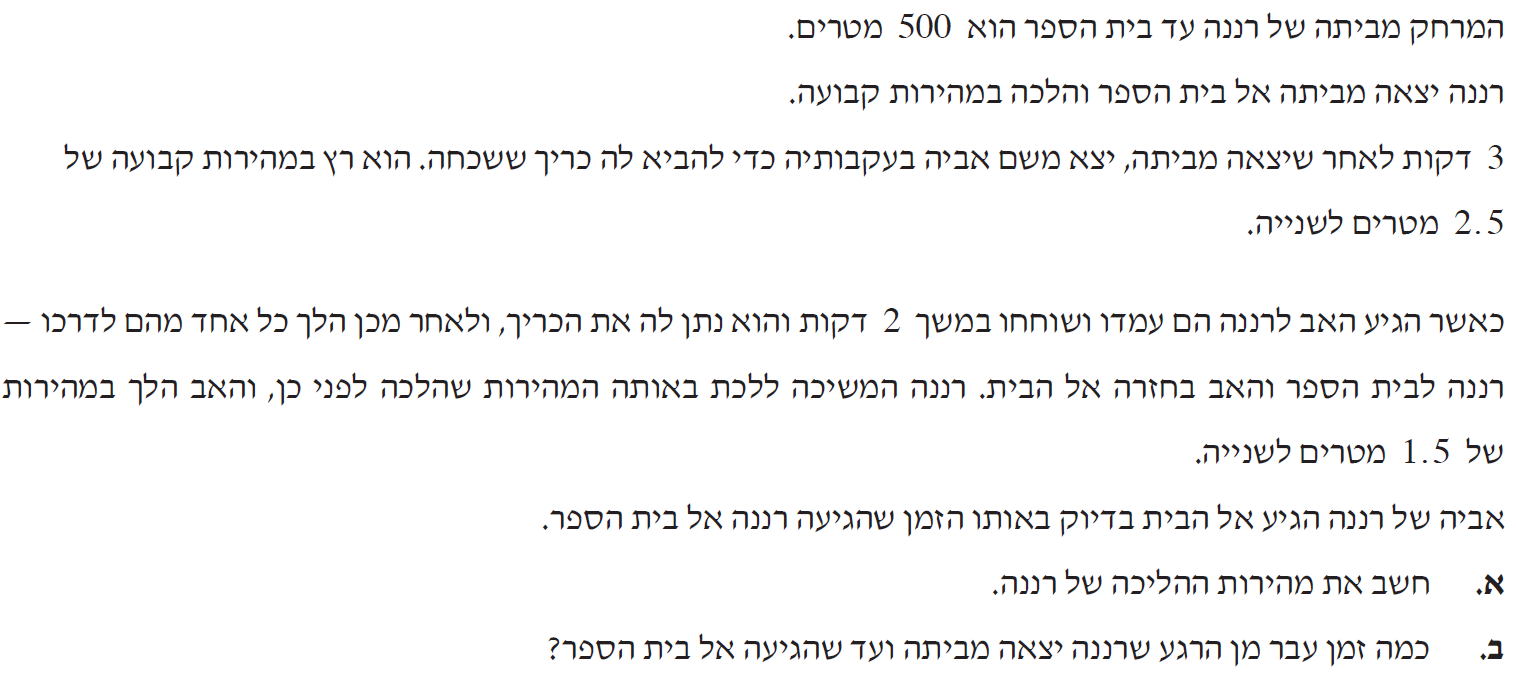
\includegraphics[width=\textwidth]{summer-2018b-1}
\end{center}

\begin{center}
\selectlanguage{english}
\begin{tikzpicture}
\draw (0,0) node[left] {$0$ } -- (10,0);
\node at (-.45,0.5) {
\R{בית}
};
\draw (0,0) -- (0,6) node[left] {$500$};
\node at (-.84,5.5) {
\R{בית ספר}
};
\draw[dashed] (0,6) -- (10,6);
\draw[thick] (0,0) -- node[above left] {
\R{רננה}
} (4.5,3);
\draw[thick] (2,0) -- node[above right,xshift=10pt,near start] {
\R{אבא}
} (4.5,3);
\draw[thick] (4.5,3) -- node[above] {
\R{רננה ואבא}
} (7,3);
\draw[thick] (7,3) -- node[above right] {
\R{אבא}
} (10,0);
\draw[thick] (7,3) -- node[above left] {
\R{רננה}
} (10,6);
\fill (4.5,3) circle [radius=2pt];
\fill (0,0) circle [radius=2pt];
\fill (2,0) circle [radius=2pt];
\fill (4.5,0) circle [radius=2pt];
\fill (7,0) circle [radius=2pt];
\fill (7,3) circle [radius=2pt];
\fill (10,0) circle [radius=2pt];
\fill (10,6) circle [radius=2pt];
\draw[dashed] (10,6) -- (10,0);
\draw[dashed] (4.5,3) -- (4.5,0);
\draw[dashed] (7,3) -- (7,0);
\draw[<->] (0,-5mm) -- node[fill=white] {$180$} (2,-5mm);
\draw[<->] (2,-5mm) -- node[fill=white] {$t$} (4.5,-5mm);
\draw[<->] (4.5,-5mm) -- node[fill=white] {$120$} (7,-5mm);
\draw[<->] (7,-5mm) -- node[fill=white] {$t'$} (10,-5mm);
\end{tikzpicture}
\end{center}

\vspace*{-1ex}

נסמן:
$=v$
מהירות ההליכה של רננה,
$=t$
הזמן עד למפגש בין רננה לאביה,
$=t'$
הזמן מהפרידה בין רננה לאביה עד ששניהם מגיעים ליעדם.

מהתרשים אפשר לראות שוויונות בין מרחקים: )א( המרחק שרננה הלכה עד למפגש שווה למרחק שאבא הלך עד למפגש, )ב( המרחק שאבא הלך עד למפגש שווה למרחק שאבא הלך בחזרה מהמפגש, )ג( המרחק לבית הספר שווה למרחק שרננה הלכה עד למפגש ועוד המרחק שהיא הלכה מהפגש עד לבית הספר.

\np

\textbf{סעיף א}

תחילה נשווה את המרחקים שאבא עובר מהבית עד למפגש ובחזרה:

\vspace{-2ex}

\erh{14pt}
\begin{equationarray*}{rcl}
\frac{5}{2}t &=& \frac{3}{2}t'\\
t' &=& \frac{2}{3}\cdot\frac{5}{2}t = \frac{5}{3}t\,.
\end{equationarray*}

\vspace{-3ex}

נמשיך בהשוואת המרחק עד למפגש של שניהם:
\[
v(t+180) = \frac{5}{2}t\,.
\]
אנו זקוקים לשתי משוואות עם שני הנעלמים כדי למצוא את
$v$.
אי-אפשר למצוא משוואה שניה מהנתונים מהמפגש עד ליעדים שלהם, כי המרחקים לא בהכרח שווים. במקום זה נמצא דרך אחרת להשוות את המרחק שעוברים רננה ואבא מהבית עד למפגש. עבור אבא נשתמש שוב ב-% 
$\frac{5}{2}t$.
עבור רננה נשים לב שניתן לחשב את המרחק המבית עד למפגש כהפרש בין המרחק מהבית לבית הספר 
$(500)$
לבין המרחק שהיא עוברת מהמפגש ועד לבית הספר
$vt'$:
\[
\frac{5}{2}t = 500 - vt'= 500 - v\left(\frac{5}{3}t\right)\,.
\]
כעת יש לנו שתי משוואת בשני הנעלמים
$v,t$.
מהראשון נחשב:
\[
t = \frac{360v}{5-2v}\,,
\]
ונציב בשני:
\[
\frac{5}{2} \left(\frac{360v}{5-2v}\right) =
500 - v\left(\frac{5}{3}\cdot\frac{360v}{5-2v}\right)\,.
\]
נפשט את המשוואה ונקבל משוואה ריבועית עבור
$v$:
\erh{2pt}
\begin{equationarray*}{rcl}
6v^2 + 19v - 25 &=& 0\\
(v-1)(6v+25)&=&0\,.
\end{equationarray*}
המהירות חייבת להיות חיובית ולכן הפרתון היחיד הוא
$v=1$.

\textbf{סעיף ב}

מ-%
$t = \disfrac{360v}{5-2v}$
נקבל
$t=120$,
ונסכם את פרקי הזמן על הציר האופקי בתרשים:
\[
180 + 120 + 120 + \frac{5}{3}\cdot 120 = 620\;\;\textrm{(\R{שניות})}.
\]
\textbf{הערה}

שימו לב למלכודת שקל ליפול לתוכה: הזמנים נתונים בדקות והמהיריויות נתונות במטרים שנייה!


%%%%%%%%%%%%%%%%%%%%%%%%%%%%%%%%%%%%%%%%%%%%%%%%%%%%%%%%%%%%%%%%

\np

\section{קיץ תשע"ח מועד א}

\begin{center}
\selectlanguage{english}
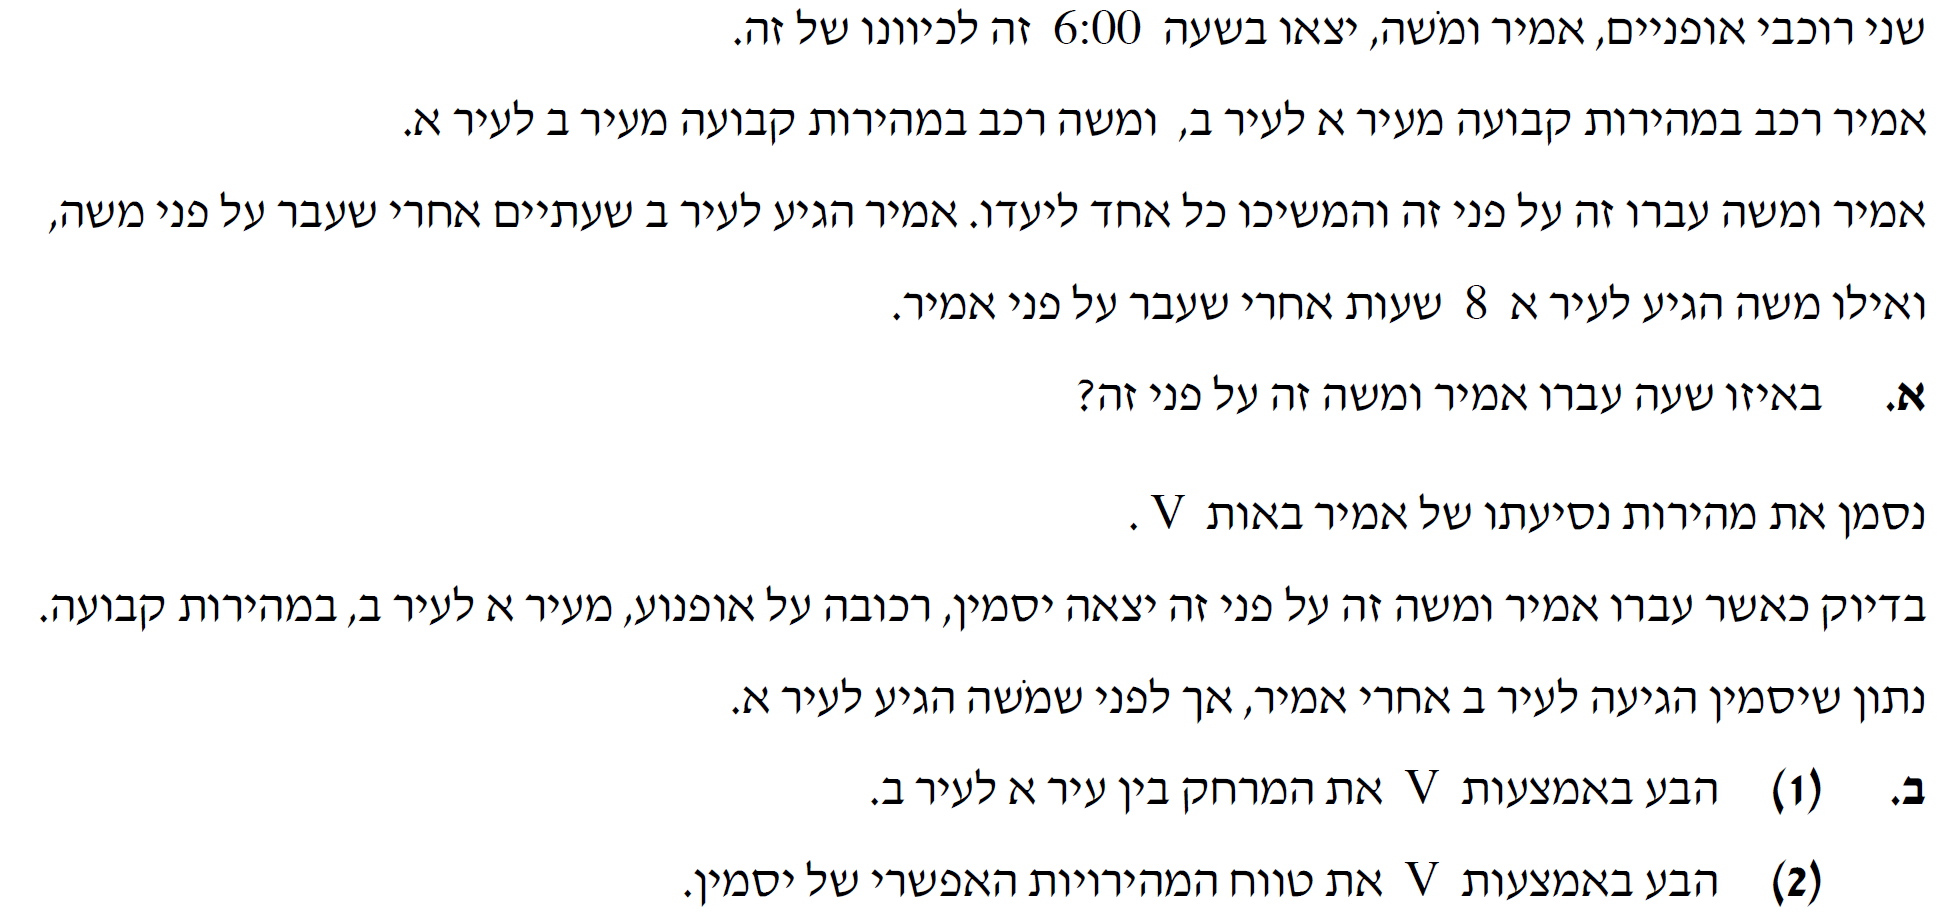
\includegraphics[width=\textwidth]{summer-2018a-1}
\end{center}

\begin{center}
\selectlanguage{english}
\begin{tikzpicture}[scale=.95]
\draw (0,0) node[left] {
\R{עיר א}
} node[below left,yshift=-6pt] {\p{06:00}} -- (10,0);
\draw (0,0) -- (0,6) node[left] {
\R{עיר ב}
};
\draw[dashed] (0,6) -- (10,6);
\draw[thick,name path=amir] (0,0) -- node[above left,near start] {
\R{אמיר}
} (6,6);
\draw[thick,name path=moshe] (0,6) -- node[above right,near start] {
\R{משה}
} (10,0);
\fill (0,6) circle [radius=2pt];
\fill (0,0) circle [radius=2pt];
\fill (6,6) circle [radius=2pt];
\fill (10,0) circle [radius=2pt];
\path[name intersections={of=amir and moshe,by=meeting}];
\fill (meeting) circle [radius=2pt];
\draw[dashed] (meeting) |- coordinate (meeting-time) (0,0);
\fill (meeting-time) circle [radius=2pt];
\draw[thick] (meeting-time) -- node[right,yshift=20pt,xshift=20pt] {
\R{יסמין}
} (8,6);
\fill (8,6) circle [radius=2pt];
\draw[dashed] (6,6) -- (6,0);
\draw[dashed] (8,6) -- (8,0);
\draw[dashed] (meeting) -| coordinate (meeting-distance) (0,0);
\fill (8,0) circle [radius=2pt];
\fill (meeting-distance) circle [radius=2pt];
\draw[<->] (0,-5mm) -- node[fill=white] {$t$} (meeting-time |- 0,-5mm);
\draw[<->] (meeting-time |- 0,-5mm) -- node[fill=white] {$2$} (6,-5mm);
\draw[<->] (meeting-time |- 0,-10mm) -- node[fill=white] {$8$} (10,-10mm);
\draw[<->] (meeting-time |- 0,-15mm) -- node[fill=white] {$t_y$} (8,-15mm);
\end{tikzpicture}
\end{center}

נסמן:
$=t$
הזמן עד למפגש בין אמיר למשה,
$=t_y$
זמן הנסיעה של יסמין מעיר א לעיר ב, 
$=v_y,v_m,v_a$
המהירויות של אמיר, משה ויסמין.


\textbf{סעיף א}

מהתרשים ניתן לראות לראות שיש
\textbf{שלושה}
ביטויים עבור המרחק בין הערים: )א( הרחק שנסע אמיר, )ב( המרחק שנסע משה, ו-)ג( סכום המרחקים שנסעו אמיר ומשה עד למפגש:
\[
tv_a + tv_m = (t+2) v_a = (t+8) v_m\,.
\]
משני הביטויים הראשונים אנו מקבלים:
\[
\frac{v_a}{v_m}=\frac{t}{2}\,.
\]

\np

נציב בשני הביטויים האחרונים:
\[
(t+2)\cdot \frac{tv_m}{2} = (t+8) v_m\,.
\]
$v_m$
מצטמצם ונקבל משוואה ריבועית
$t^2-16$
עם הפתרון החיובי 
$t=4$.

\textbf{שימו לב}

יש נטייה לעצור כאן כאשר חישבנו את הזמן 
$t$,
אבל עיון חוזר בשאלה מראה שהיא מבקשת את
\textbf{השעה}
של המפגש שהיא
\L{\p{10:00}}.

\smallskip

\textbf{סעיף ב}

המרחק בין הערים הוא 
$(t+2)v_a$.
חישבנו ש-%
$t=4$
ולכן המרחק הוא
$6v_a=6V$
)הסימון הנתון 
$V$
שונה מ-%
$v_a$
שבחרתי(.


\smallskip

\textbf{סעיף ג}

נתון שיסמין מגיע לעיר ב אחרי אמיר ולפני משה. מהתרשים רואים ש:
\[
2 < t_y < 8\,.
\]
זמן הוא מרחק חלקי מהירות ואת המרחק חישבנו בסעיף ב:
\[
2 < \frac{6V}{v_j} < 8\,.
\]
מכאן ש:
\[
\frac{3}{4}V < v_j < 3V\,
\]
כי כיווני האי-שוויון מתחלפים עם היפוך השבר.

%%%%%%%%%%%%%%%%%%%%%%%%%%%%%%%%%%%%%%%%%%%%%%%%%%%%%%%%%%%%%%%%

\np

\section{חורף תשע"ח}

\begin{center}
\selectlanguage{english}
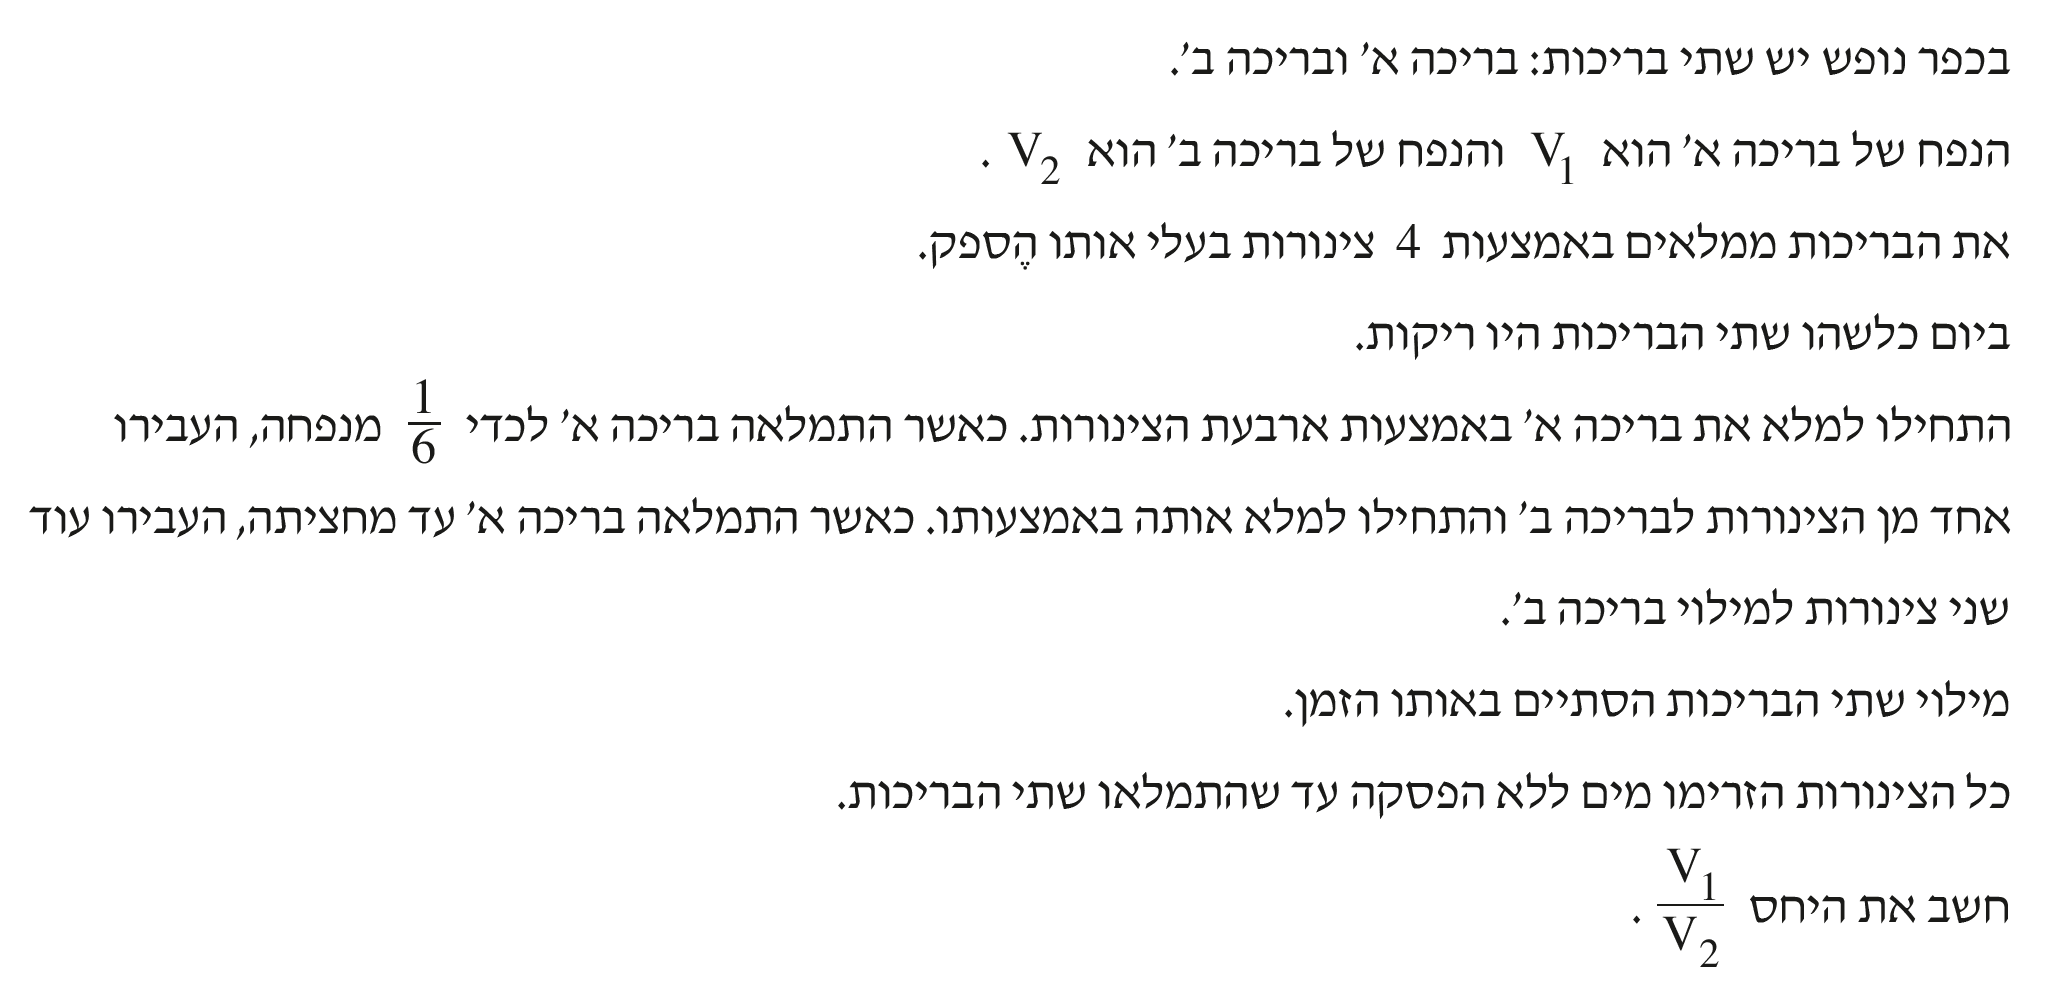
\includegraphics[width=\textwidth]{winter-2018-1}
\end{center}

\begin{center}
\selectlanguage{english}
\begin{tikzpicture}[scale=1]
\draw (0,0) node[left] {$0$} -- (10,0);
\draw (0,0) -- (0,6);
\node at (-.5,1) {$\frac{1}{6}V_1$};
\node at (-.5,3) {$\frac{1}{2}V_1$};
\node at (-.5,6) {$V_1$};

\fill (0,0) circle [radius=2pt];
\draw[dashed] (0,1) -- (1,1);
\draw (0,0) -- node[below,xshift=4pt] {$4x$} (1,1);
\fill (1,1) circle [radius=2pt];

\draw[dashed] (0,3) -- (4,3);
\draw (1,1) -- node[below,xshift=4pt] {$3x$} (4,3);
\fill (4,3) circle [radius=2pt];

\draw[dashed] (0,6) -- (10,6);
\draw (4,3) -- node[below,xshift=4pt] {$x$} (10,6);
\fill (10,6) circle [radius=2pt];

\draw[dashed] (1,1) -- (1,0);
\draw[dashed] (4,3) -- (4,0);
\draw[dashed] (10,6) -- (10,0);

\draw[<->] (10.5,0) -- node[fill=white] {$V_2$} (10.5,5.5);

\fill (1,0) circle [radius=2pt];
\draw (1,0) -- node[below,xshift=4pt] {$x$} (4,1);
\fill (4,1) circle [radius=2pt];
\draw (4,1) -- node[below,xshift=4pt] {$3x$} (10,5.5);
\fill (10,5.5) circle [radius=2pt];

\draw[<->] (0,-.5) -- node[fill=white] {$t_1$} (1,-.5);
\draw[<->] (1,-.5) -- node[fill=white] {$t_2$} (4,-.5);
\draw[<->] (4,-.5) -- node[fill=white] {$t_3$} (10,-.5);


\end{tikzpicture}
\end{center}


נסמן:
$=x$
קצב המילוי של הצינורות )"אותו הספק"(,
$=t_1, t_2, t_3$
פרקי הזמן בין העברת הצינורות.

הקו העליון בתרשים מתאר את המילוי של בריכה א, והקו התחתון מתאר את מילוי של בריכה ב. שימו לב שככל שיותר צינורות ממלאים בריכה, השיפוע של הקו תלול יותר.

יש לנו שלוש קבונות של נעלמים: 
$x$,
שלושת ה-%
$t_i$
ושני ה-%
$V_i$.
אם נצליח להיפטר מ-%
$x$
או מה-%
$t_i$,
השני יצטמצם כאשר נחלק את ה-%
$V_i$.

נתחיל עם משוואות ההספק עבור בריכה א, כאשר בכל פרק זמן ממלאים את ההפרשים של הנפחים, למשל, בזמן 
$t_2$
בריכה א מתמלאת מששית מנפחה לחצי מנפחה:
\np
\erh{12pt}
\begin{equationarray*}{rcl}
4x t_1 &=& \frac{1}{6}V_1\\
3x t_2 &=& \left(\frac{1}{2}-\frac{1}{6}\right)V_1\\
xt_3&=&\left(1-\frac{1}{2}\right)V_1\,.
\end{equationarray*}
נשתמש במשוואת כדי לחשב את פרקי הזמן כתלות בנפח בבריכה:
\erh{12pt}
\begin{equationarray*}{rcl}
t_1 &=& \frac{V_1}{24x}\\
t_2 &=& \frac{V_1}{9x}\\
t_3&=&\frac{V_1}{2x}\,.
\end{equationarray*}
מהתרשים רואים שאפשר לבטא את הנפח של
$V_2$
כסכום: הנפח שמתמלא בפרק הזמן
$t_2$
ועוד הנפח המתמלא בפרק הזמן
$t_3$.
כאשר נציב את המשוואות שקבלנו עבור בפרקי הזמן, נקבל את הנפח של
$V_2$
כתלות ב-%
$V_1$
בלבד, כי המשתנה 
$x$ מצטמצם:
\erh{12pt}
\begin{equationarray*}{rcl}
V_2 &=& xt_2 + 3xt_3 = \frac{x V_1}{9x} + \frac{3x V_1}{2x}\ = \frac{29}{18}V_1\\
\frac{V_1}{V2} &=& \frac{18}{29}\,.
\end{equationarray*}
\textbf{הערה}

קיבלנו שהנפח של בריכה ב גדול מהנפח של בריכה א, עובדה שלא ידעתי כאשר ציירתי את התרשים עם נפח בריכה א גדול מנפח בריכה ב! אין לזה חשיבות. מטרת התרשים היא להציג את התסריט כדי שנוכל לכתוב את המשוואות הנכונות. 

פרט מעניין הוא שפרק הזמן הראשון
$t_1$
לא נחוץ לפתרון, כי המילוי של בריכה ב מתבצע בשני השלבים לאחר העברת הצינור הראשון.

%%%%%%%%%%%%%%%%%%%%%%%%%%%%%%%%%%%%%%%%%%%%%%%%%%%%%%%%%%%%%%%%

\np

\section{קיץ תשע"ז מועד ב}

\begin{center}
\selectlanguage{english}
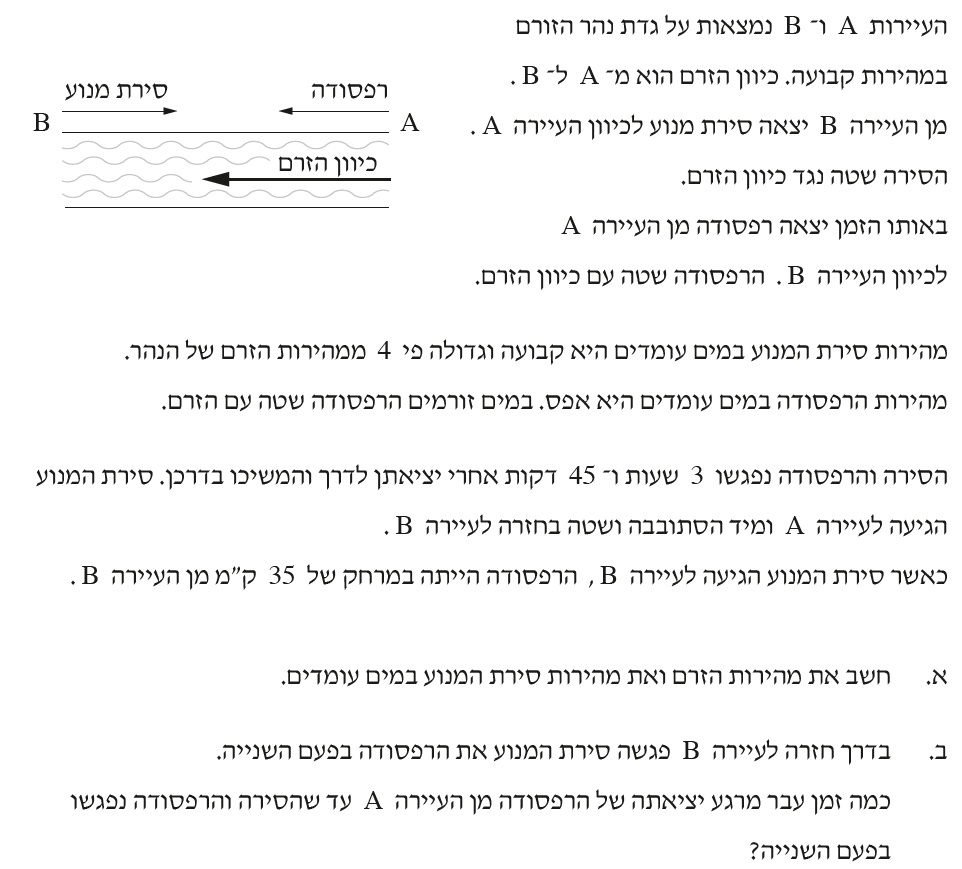
\includegraphics[width=.95\textwidth]{summer-2017b-1}
\end{center}

\vspace{-2ex}

\textbf{סעיף א}

\vspace{-3ex}

\begin{center}
\selectlanguage{english}
\begin{tikzpicture}[scale=.9]
\draw[name path=xaxis] (0,0) node[below left] {$A$} -- (10,0);
\draw (0,0) -- (0,6) node[above left] {$B$};
\draw[dashed] (0,6) -- (10,6);
\draw[thick,name path=raft] (0,0) -- node[left,near start,xshift=-4pt] {
\R{רפסודה}
} (10,4.5);
\draw[thick,name path=boat1] (0,6) -- node[right,near start,xshift=2pt] {
\R{סירה}
} (7,0);
\draw[thick,name path=boat2] (7,0) -- (10,6);
\path [name intersections={of=boat1 and raft,by=meeting1}];
\draw[dashed] (meeting1) |- coordinate (time) (0,0);
\draw[dashed] (meeting1) -| coordinate (distance) (0,0);
\draw[dashed] (10,0) -- (10,6);
\path[name path=t1] (7,0) -- (7,6);
\path [name intersections={of=raft and t1,by=a}];
\path [name intersections={of=raft and boat2,by=meeting2}];
\fill (meeting1) circle [radius=2pt];
\fill (meeting2) circle [radius=2pt];
\path [name path=t2] (meeting2) |- (0,0);
\path [name intersections={of=xaxis and t2,by=t2x}];
\fill (time) circle [radius=2pt];
\fill (0,0) circle [radius=2pt];
\fill (7,0) circle [radius=2pt];
\fill (10,6) circle [radius=2pt];
\fill (10,4.5) circle [radius=2pt];
\fill (0,6) circle [radius=2pt];
\fill (distance) circle [radius=2pt];
\draw[<->] (-.4,0) -- node[fill=white] {$d_r$} (distance -| -.4,0);
\draw[<->] (distance -| -.4,0) -- node[fill=white] {$d_s$} (-.4,6);
\draw[<->] (-.9,0) -- node[fill=white] {$d$} (-.9,6);
\draw[<->] (0,-.6) -- node[fill=white] { $15/4$} (time |- 0,-.6);
\draw[<->] (10.4,4.5) -- node[fill=white] { $35$} (10.4,6);
\end{tikzpicture}
\end{center}
נסמן:
$=d$
המרחק בין שני הנמלים,
$=d_r, d_s$
מרחקי ההפלגה של הסירה והרפסודה עד למפגש הראשון,
$=v_z$
מהירות הזרם,
$=v_s$
מהירות הסירה במים עומדים. ציר הזמן הוא בשעות.

\np

הזמן עד למפגש הראשון שווה עבור הסירה והרפסודה ויחס המהירויות של הסירה והזרם ידוע, כך שניתן לכתוב את משוואות התנועה עד למפגש. נתון:
\[
v_z = v_s/4\,.
\]
במפגש הראשון:
\[
d=d_s+d_r=\frac{15}{4}(v_s-v_z) + \frac{15}{4}v_z\,.
\]
מהירות הזרם מתאפסת ומתקבל:
\[
d = \frac{15}{4}v_s\,.
\]
כעת נכתוב משוואות תנועה כדי להשוות את הזמנים עד סוף הסיפור. בפרק הזמן שהסירה מפליגה ל-%
$A$
ובחזרה ל-%
$B$
)מרחק של
$d+d$(,
הרפסודה מפליגה מ-%
$A$
ומגיעה "כמעט" לנמל
$B$:
\[
\frac{d}{v_s-v_z} + \frac{d}{v_s+v_z} = \frac{d-35}{v_z}\,.
\]
מהנתון על יחס המהירויות ומחישוב המרחק, נציב עבור 
$v_z$
ו-%
$d$,
ונקבל משוואה עם נעלם אחד בלבד,
$v_s$.
הפתרון הוא
$v_s=20$
ומיחס המהירויות
$v_z=5$.
נחשב גם
$d=75$
שנצטרך בהמשך.

\smallskip

\textbf{סעיף ב}

נצייר תרשים חדש עם סימונים הקשורים למפגש השני.

\vspace{-1ex}

\begin{center}
\selectlanguage{english}
\begin{tikzpicture}[scale=.9]
\draw[name path=xaxis] (0,0) node[below left] {$A$} -- (10,0);
\draw (0,0) -- (0,6) node[above left] {$B$};
\draw[dashed] (0,6) -- (10,6);
\draw[thick,name path=raft] (0,0) -- node[left,near start,xshift=-4pt] {
\R{רפסודה}
} (10,4.5);
\draw[thick,name path=boat1] (0,6) -- node[right,near start,xshift=2pt] {
\R{סירה}
} (7,0);
\draw[thick,name path=boat2] (7,0) -- (10,6);
\path [name intersections={of=boat1 and raft,by=meeting1}];
\draw[dashed] (10,0) -- (10,6);
\path[name path=t1] (7,0) -- (7,6);
\path [name intersections={of=raft and t1,by=a}];
\path [name intersections={of=raft and boat2,by=meeting2}];
\fill (meeting2) circle [radius=2pt];
\fill (a) circle [radius=2pt];
\draw[<->] (7,.15) -- node[fill=white] {$d'$} (a);
\path [name path=t2] (meeting2) |- (0,0);
\fill (a -| meeting2) circle [radius=2pt];
\path [name intersections={of=xaxis and t2,by=t2x}];
\draw[<->] (a -| meeting2) -- node[fill=white,right,xshift=2pt] {$d''$} (meeting2);
\draw[dashed] (a -| meeting2) -- (t2x);
\draw[dashed] (a) -- (a -| meeting2) coordinate (one);
\fill (t2x) circle[radius=2pt];
\fill (0,0) circle [radius=2pt];
\fill (7,0) circle [radius=2pt];
\fill (10,6) circle [radius=2pt];
\fill (10,4.5) circle [radius=2pt];
\draw[<->] (0,-.4) -- node[fill=white] {$t_1$} (7,-.4);
\draw[<->] (7,-.4) -- node[fill=white] {$t_2$} (7,-.4 -| t2x);
\end{tikzpicture}
\end{center}

\vspace{-1ex}


נסמן:
$=t_1$
הזמן שהסירה מפליגה ל-%
$A$
ל-%
$B$,
$=t_2$
הזמן שהסירה מפליגה מ-%
$A$
למפגש השני,
$=d'$
המרחק שהרפסודה מפליגה בזמן
$t_1$,
$=d''$
המרחק שהרפסודה מפליגה בזמן
$t_2$.

\smallskip
קל לחשב
$t_1$
ממשוואת התנועה של הסירה:
\[
t_1=\frac{d}{v_s-v_z}=\frac{75}{20-5}=5\,,
\]

ולחשב את המרחק
$d'$
מהמשוואה של הרפסודה:
\[
d'=v_zt_1=5\cdot 5=25\,.
\]

\np

נשאר לחשב את פרק הזמן
$t_2$.
בפרק זמן זה הסירה מפליגה מרחק
$d'+d''$
והרפסודה מפליגה מרחק
$d''$.
המהירויות ידועות, כך שיש לנו שתי משוואות עבור
$t_2$:
\erh{14pt}
\begin{equationarray*}{rcl}
t_2&=&\frac{d'+d''}{v_s+v_z} = 
\frac{25+d''}{25}\\
t_2&=&\frac{d''}{v_z}=\frac{d''}{5}\,.
\end{equationarray*}
נפתור את המשוואה ונקבל:
\erh{14pt}
\begin{equationarray*}{rcl}
d''&=&\frac{25}{4}\\
t_2&=&\frac{d''}{v_z}=\frac{5}{4}\,.
\end{equationarray*}
\textbf{שימו לב}

שהשאלה מבקשת את זמן ההפלגה של הרפסודה מנמל
$A$
ועד למפגש השני:
\[
t_1+t_2=5+\frac{5}{4}=\frac{25}{4}\,.
\]


%%%%%%%%%%%%%%%%%%%%%%%%%%%%%%%%%%%%%%%%%%%%%%%%%%%%%%%%%%%%%%%%

\np

\section{קיץ תשע"ז מועד א}

\begin{center}
\selectlanguage{english}
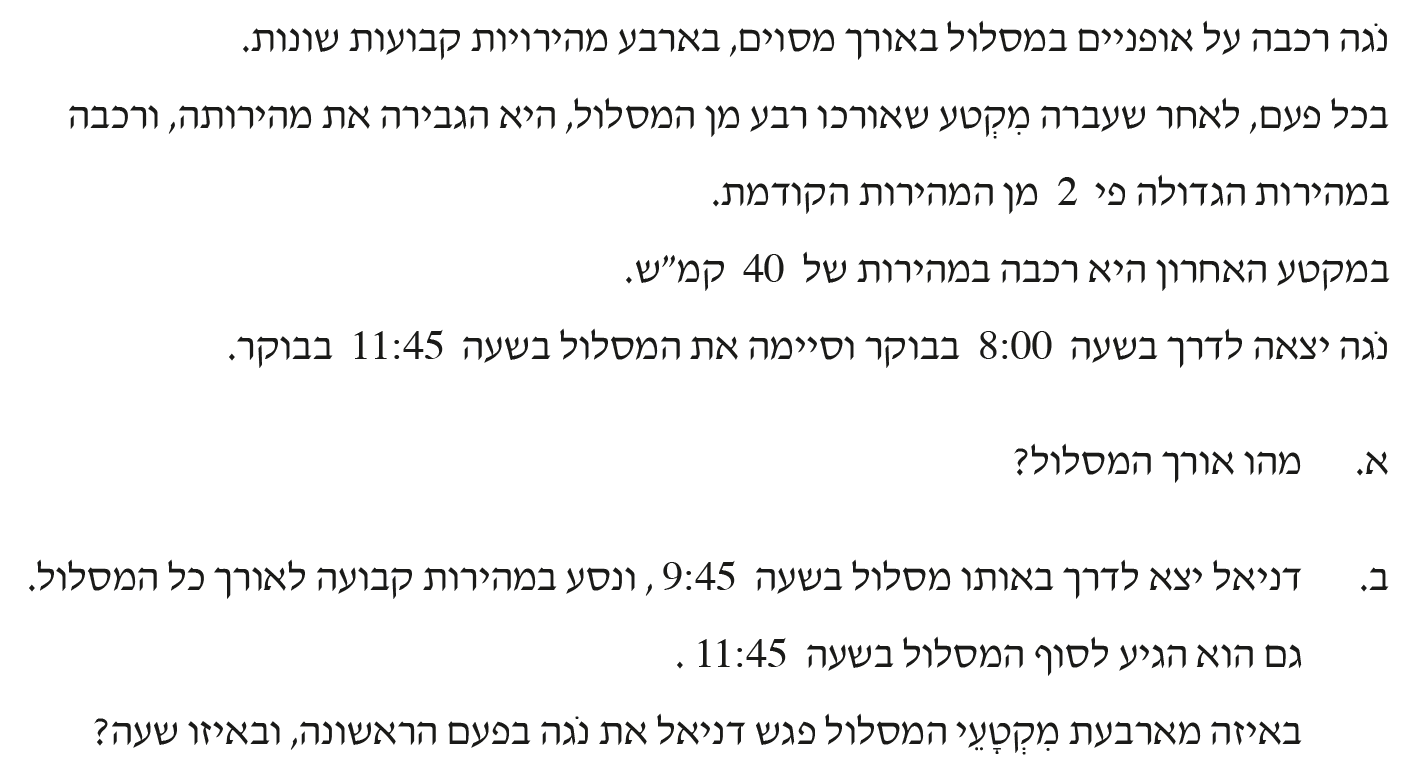
\includegraphics[width=\textwidth]{summer-2017a-1}
\end{center}

\begin{center}
\selectlanguage{english}
\begin{tikzpicture}[scale=1]
\draw (0,0) node[below] {\p{08:00}} -- (11.25,0) node[below] {\p{11:45}};
\draw (0,0) -- (0,6);
\draw[thick,name path=noga] (0,0) -- (6,1.5) -- (9,3) -- (10.5,4.5) --  node[right] {
\R{נגה}
} (11.25,6);
\draw[dashed] (0,6) -- +(11.25,0);
\draw[dashed] (0,4.5) -- +(10.5,0);
\draw[dashed] (0,3) -- +(9,0);
\draw[dashed] (0,1.5) -- +(6,0);
\draw[dashed] (6,0) -- (6,1.5);
\draw[dashed] (9,0) -- (9,3);
\draw[dashed] (10.5,0) -- (10.5,4.5);
\draw[dashed] (11.25,0) -- (11.25,6);
\fill (0,0) circle [radius=2pt];
\fill (6,1.5) circle [radius=2pt];
\fill (9,3) circle [radius=2pt];
\fill (10.5,4.5) circle [radius=2pt];
\fill (11.25,6) circle [radius=2pt];
\path (0,0) -- node[left] {$x$} (0,1.5) -- node[left] {$x$} (0,3) -- node[left] {$x$} (0,4.5) -- node[left] {$x$} (0,6);
\draw[thick,name path=dan] (5.25,0) node[below] {\p{09:45}} --  node[left,xshift=16pt,yshift=20pt] {
\R{דניאל}
} (11.25,6);
\path [name intersections={of=noga and dan,by=meeting}];
\draw[dashed] (meeting) |- coordinate (time) (0,0);
\fill (5.25,0) circle [radius=2pt];
\fill (meeting) circle [radius=2pt];
\fill (time) circle [radius=2pt];
\draw[<->] (0,-7mm) -- node[below] {$t_1$} +(6,0);
\draw[<->] (6,-7mm) -- node[below] {$t_2$} +(3,0);
\draw[<->] (6,3mm) -- node[above] {$t$} (time |- 6,3mm);
\draw[<->] (9,-7mm) -- node[below] {$t_3$} +(1.5,0);
\draw[<->] (10.5,-7mm) -- node[below] {$t_4$} +(.75,0);
\end{tikzpicture}
\end{center}

נסמן:
$=x$
המרחק של מקטע,
$=t_1,t_2,t_3,t_4$
זמני רכיבה של נגה במקטעים.

נתון: 
$=40$
המהירות במקטע האחרון, לכן המהירויות של המקטעים האחרים הן
$5,10,20$.

\textbf{סעיף א}

נתון לנו הזמן הכולל והמהירויות )אמנם רק המהירות האחרונה נתונה, אבל אפשר לחשב את האחרות(, והנעלם היחיד הוא המרחק. נסכם את הזמנים של המקטעים:
\[
\left(\frac{x}{5}+\frac{x}{10}+\frac{x}{20}+\frac{x}{40}\right) = \frac{15}{4}\,.
\]
הפתרון הוא
$x=10$
ולכן אורך המסלול הוא
$40$
ק"מ.

\np

\textbf{סעיף ב}

חישבנו את המרחק ונתון הזמן של דניאל. המהירות של דניאל היא 
$40/2=20$
קמ"ש.

אפשר אולי למצוא נוסחה עבור המפגש, אבל פשוט יותר לעבור מקטע מקטע ולבדוק אם המפגש מתקיים באותו מקטע.

נגה עוברת
$10$
ק"מ בכל מקטע. מה המרחק שעובר דניאל עד סוף המקטע הראשון?

$t_1 = 10/5 = 2$
כך שסוף המקטע הוא ב- 
\L{\p{10:00}}.
דניאל רוכב רבע שעה מ-
\L{\p{09:45}}
ועד
\L{\p{10:00}}
ולכן המרחק שהוא עובר הוא רק
$\displaystyle 20\cdot\frac{1}{4} = 5$
ק"מ והמפגש לא התקיים במקטע הראשון.


מתי נגה מגיעה לסוף המקטע השני?
$t_2=10/10 =1$
כך שסוף המקטע הוא ב-%
\L{\p{11:00}}.
בשעה ורבע בין 
\L{\p{09:45}}
ל
\L{\p{11:00}}
דניאל רוכב
$\displaystyle 20\cdot \frac{5}{4}=25$
ק"מ, מרחק גדול מהמרחק של נגה, לכן המפגש מתקיים במקטע השני.

\medskip

נשאר רק לחשב את פרק הזמן בתוך המקטע השני עד למפגש, שנסמן
$t$.
נכתוב משוואה למרחקים השווים של נגה ודניאל. נגה רכבה
$10$
ק"מ עד סוף הקטע הראשון ודניאל רכב 
$5$
ק"מ. מסוף הקטע הראשון, הם רכבו 
$t$
שעות, כל אחד במהירות שלו:
\erh{12pt}
\begin{equationarray*}{rcl}
10 + 10t &=& 5 + 20t\\
t&=&\frac{1}{2}\,.
\end{equationarray*}
\textbf{שימו לב}

השאלה מבקשת את שעת המפגש. כבר חישבנו שתחילת המקטע השני בשעה
\L{\p{10:00}},
ולכן שעת המפגש היא
\L{\p{10:30}}.

%%%%%%%%%%%%%%%%%%%%%%%%%%%%%%%%%%%%%%%%%%%%%%%%%%%%%%%%%%%%%%%%

\np

\section{חורף תשע"ז}

\begin{center}
\selectlanguage{english}
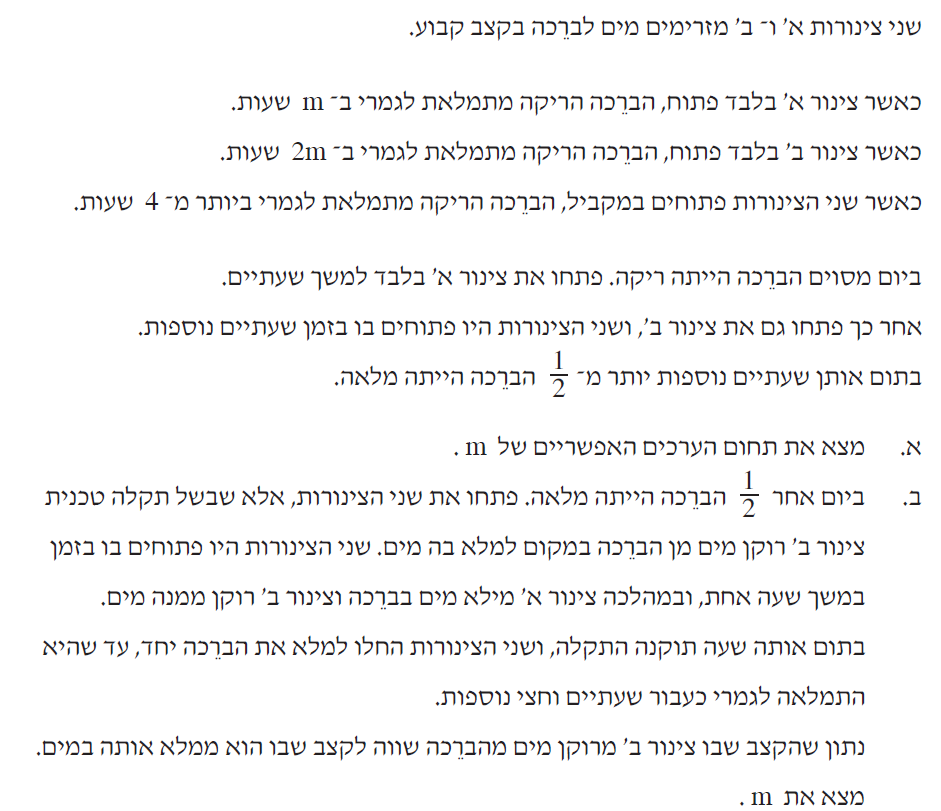
\includegraphics[width=.9\textwidth]{winter-2017-1}
\end{center}

%\vspace{-3ex}

\textbf{סעיף א}

\begin{center}
\selectlanguage{english}
\begin{tikzpicture}[scale=.8]
\draw (0,0) -- (10,0);
\draw (0,0) node[left] {\R{בריכה ריקה}} -- (0,6) node[left] {\R{בריכה מליאה}};
\draw[dashed] (0,6) -- (10,6);
\draw[thick] (0,0) -- node[right,near end,xshift=2mm,yshift=-2mm] {
\R{ב}
} node[right,xshift=12mm,yshift=4mm] {$\displaystyle\frac{1}{2m}$}(9,6);
\draw[thick] (0,0) -- node[left,near end,xshift=-3mm] {
\R{א}
} node[left,xshift=-2mm,yshift=3mm] {$\displaystyle\frac{1}{m}$} (4.5,6);
\draw[dashed] (9,6) -- (9,0);
\draw[dashed] (4.5,6) -- (4.5,0);
\draw[<->] (0,-.6) -- node[fill=white] {$m$} (4.5,-.6);
\draw[<->] (0,-1.2) -- node[fill=white] {$2m$} (9,-1.2);
\end{tikzpicture}
\end{center}

%\vspace{-2ex}

כאשר שני הצינורות פתוחים, ההספק הכולל הוא סכום ההספקים של הצינורות. לפי הנתונים:
\[
1/\left(\frac{1}{m}+\frac{1}{2m}\right) > 4\,,
\]
כך ש-%
$m>6$.

\np

\begin{center}
\selectlanguage{english}
\begin{tikzpicture}
\draw (0,0) -- (10,0);
\draw (0,0) node[left] {\R{בריכה ריקה}}
-- (0,4) node[left] {\R{בריכה מליאה}};
\draw[thick] (4,0) -- node[above,near end,yshift=2mm] {
\R{ב}
} node[above,near start,yshift=2mm] {$\displaystyle\frac{1}{2m}$}(8,1);
\draw[thick] (0,0) -- node[left,near end,xshift=-3mm] {
\R{א}
} node[left,xshift=-2mm,yshift=3mm] {$\displaystyle\frac{1}{m}$} (8,4);
\draw[dashed] (8,4) -- (8,0);
\draw[dashed] (4,2) -- (4,0);
\draw[<->] (0,-.6) -- node[fill=white] {$2$} (4,-.6);
\draw[<->] (0,-1.2) -- node[fill=white] {$4$} (8,-1.2);
\draw[<->] (9,0) -- node[fill=white] {$w_a$} (9,4);
\draw[<->] (8.5,0) -- node[fill=white] {$w_b$} (8.5,1);
\end{tikzpicture}
\end{center}
נסמן:
$=w_a$
כמות המים שמילא צינור א,
$=w_b$
כמות המים שמילא צינור ב.

\smallskip

כמות המים לאחר ארבע שעות שווה לסכום הכמויות שכל צינור מילא והיא לפחות מחצית הבריכה:
\[
w_a + w_b = \frac{1}{m}\cdot 4 + \frac{1}{2m}\cdot 2 > \frac{1}{2}\,.
\]
מכאן,
$m<10$.

\smallskip

\textbf{סעיף ב}

\begin{center}
\selectlanguage{english}
\begin{tikzpicture}[scale=.9]
\draw (0,0) -- (9,0);
\draw (0,0) node[left] {\R{בריכה ריקה}}
-- (0,6) node[left] {\R{בריכה מליאה}};
\draw[dashed] (0,6) -- (9,6);
\draw[thick] (0,3) -- node[below right,xshift=10mm,yshift=-4mm] {$\displaystyle\frac{1}{m}-\frac{1}{2m}=\frac{1}{2m}$} (2,3.5);
\draw[->] (2.2,2.15) -- +(140:1.6cm);
\draw[thick] (2,3.5) -- node[left,xshift=-4mm,yshift=3mm] {$\displaystyle\frac{1}{m}+\frac{1}{2m}=\frac{3}{2m}$} (7,6);
\draw[dashed] (2,3.5) -- (2,0);
\draw[dashed] (2,3.5) -- (0,3.5);
\draw[dashed] (7,6) -- (7,0);
\draw[<->] (0,-.6) -- node[fill=white] {$1$} (2,-.6);
\draw[<->] (2,-1.2) -- node[fill=white] {$2.5$} (7,-1.2);
\node at (-.4,3) {$\displaystyle\frac{1}{2}$};
\end{tikzpicture}
\end{center}
כדי למלא את הבריכה, מתחילים ממחצית הכמות, מוסיפים )מחסירים כי שלילי( את הכמות של השעה הראשונה, ומוסיפים את הכמות מפרק הזמן השני של שעתיים וחצי:
\[
\frac{1}{2} + \left(\frac{1}{m}-\frac{1}{2m}\right)\cdot 1 + \left(\frac{1}{m}+\frac{1}{2m}\right)\cdot 2.5 = 1\,.
\]
הפתרון הוא
$m=8.5$.

%%%%%%%%%%%%%%%%%%%%%%%%%%%%%%%%%%%%%%%%%%%%%%%%%%%%%%%%%%%%%%%%

\np

\section{קיץ תשע"ו, מועד ב}

\begin{center}
\selectlanguage{english}
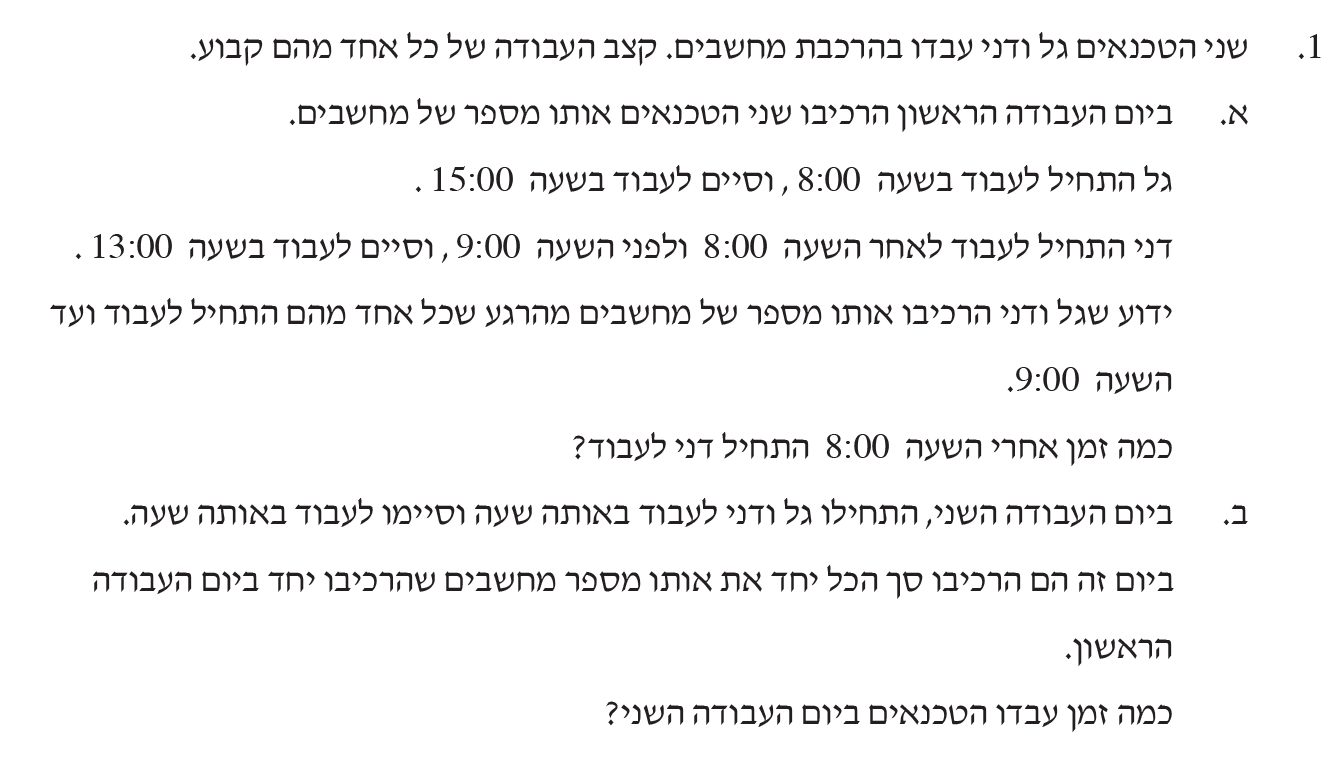
\includegraphics[width=\textwidth]{summer-2016b-1}
\end{center}

\textbf{סעיף א}

\begin{center}
\selectlanguage{english}
\begin{tikzpicture}
\draw (0,0) -- (10,0);
\draw (0,0) node[above left] {\R{אף מחשב לא הורכב}}
-- (0,6) node[left] {\R{כל המחשבים הורכבו}};
\draw[dashed] (0,6) -- (10,6);
\draw[thick,name path=gal] (0,0) -- node[right,near end,xshift=3mm] {
\R{גל}
} node[right,xshift=7mm] {$\displaystyle\frac{1}{7}$}(10,6);
\draw[thick,name path=danny] (1.2,0) -- node[left,near end,xshift=-3mm] {
\R{דני}
} node[left,yshift=3mm] {$\displaystyle\frac{1}{(1-t)+4}$} (7,6);
\draw[dashed] (7,6) -- (7,0);
\draw[dashed] (10,6) -- (10,0);
\path [name intersections={of=gal and danny,by=inter}];
\fill (inter) circle [radius=2pt];
\draw[dashed] (inter) -- (inter |- 0,0);
\draw[dashed] (inter) -- (inter -| 0,0);
\node[below] at (0,0) {\p{08:00}};
\node[below] at (1.2,0) {$t$};
\node[below] at (inter |- 0,0) {\p{09:00}};
\node[below] at (7,0) {\p{13:00}};
\node[below] at (10,0) {\p{15:00}};
\end{tikzpicture}
\end{center}

נסמן:
$=t$
הזמן שדני התחיל בהרכבה.

נשתמש בנתונים כדי למצוא ביטויים עבור ההספקים של דני וגל. נתייחס לסך המחשבים שהרכיב כל אחד כיחידת עבודה אחת. גל עבד שבע שעות ולכן ההספק שלו הוא
$\displaystyle \frac{1}{7}$,
ודני עבד 
$1-t$
עד לשעה 
\L{\p{09:00}}
ואחר כך עוד ארבע שעות. ההספק שלו הוא
$\displaystyle \frac{1}{(1-t)+4}$.

\np
נתון שבשעה 
\L{\p{09:00}}
שניהם סיימו להרכיב אותו כמות של מחשבים:
\[
\frac{1}{7}\cdot 1 = \frac{1}{(1-t)+4} \cdot (1-t)\,,
\]
ולכן דני התחיל לעבוד
$\displaystyle t=\frac{1}{3}$
שעה לאחר
\L{\p{08:00}}.

\smallskip

\textbf{סעיף ב}

נצייר תרשים חדש עם המידע הרלוונטי לסעיף זה.

\begin{center}
\selectlanguage{english}
\begin{tikzpicture}
\draw (0,0) -- (10,0);
\draw (0,0) node[above left] {\R{אף מחשב לא הורכב}}
-- (0,6) node[left] {\R{כל המחשבים הורכבו}};
\draw[dashed] (0,6) -- (10,6);
\draw[thick] (0,0) -- node[right,near end,xshift=2mm,yshift=-2mm] {
\R{גל}
} node[right,xshift=6mm,yshift=-3mm] {$\displaystyle\frac{1}{7}$}(8,2.5);
\draw[thick] (0,0) -- node[left,near end,xshift=-3mm] {
\R{דני}
} node[left,xshift=-2mm,yshift=3mm] {$\displaystyle\frac{3}{14}$} (8,6);
\draw[dashed] (8,6) -- (8,0);
\draw[<->] (0,-.6) -- node[fill=white] {$T$} (8,-.6);
\draw[<->] (8.6,0) -- node[fill=white] {$w_g$} (8.6,2.5);
\draw[<->] (9.2,0) -- node[fill=white] {$w_d$} (9.2,6);
\end{tikzpicture}
\end{center}
נסמן: 
$=T$
הזמן ששניהם עבדו ביום השני. על התרשים סימנו גם את כמות העבודה שעשה כל אחד מהם:
$=w_g$
העבודה של גל,
$=w_d$
העבודה של דני.

\smallskip

בסעיף א הערנו שההספק של גל הוא
$\displaystyle \frac{1}{7}$,
וחישבנו שדני עבד:
\[
\left(1-\frac{1}{3}\right)+4=\frac{14}{3}
\]
שעות. ההספק שלו הוא:
\[
\frac{1}{\frac{14}{3}}=\frac{3}{14}\,.
\]
נתון שהם סיימו אותה כמות עבודה כמו היום הראשון:
\[
1+1=w_g+w_d=\frac{1}{7}T + \frac{3}{14}T\,,
\]
והפתרון הוא 
$T=\displaystyle \frac{28}{5}$.

%%%%%%%%%%%%%%%%%%%%%%%%%%%%%%%%%%%%%%%%%%%%%%%%%%%%%%%%%%%%%%%%

\np

\section{קיץ תשע"ו מועד א}

\begin{center}
\selectlanguage{english}
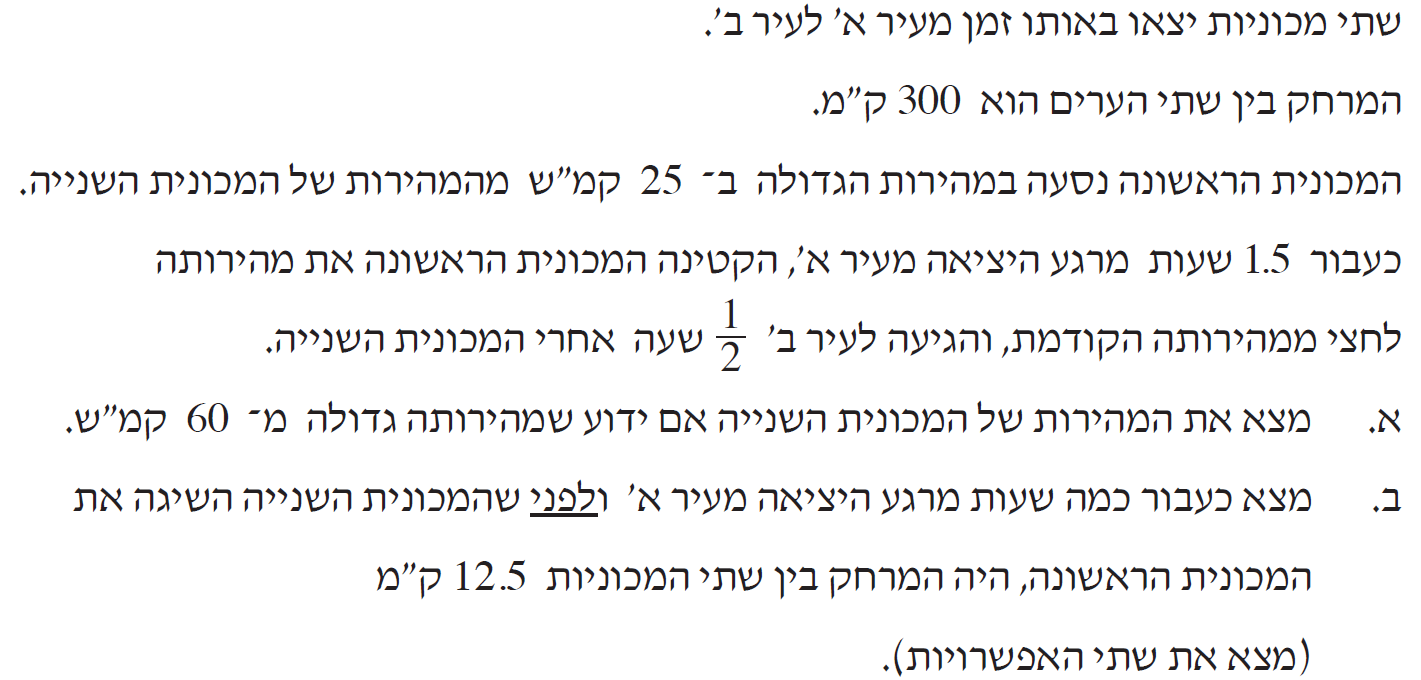
\includegraphics[width=.9\textwidth]{summer-2016a-1}
\end{center}

\begin{center}
\selectlanguage{english}
\begin{tikzpicture}
\draw (0,0) node[left] {
\R{א}
} -- (10,0);
\draw (0,0) -- node[left] {
\R{ק"מ}
$300$} (0,6) node[left] {
\R{ב}
};
\draw[dashed] (0,6) -- (10,6);
\draw[thick,name path=car1] (0,0) -- (3,4) coordinate (change) -- node[above left,near start] {$1$
\R{מכונית}
} (10,6);
\draw[thick,name path=car2] (0,0) -- node[right,xshift=1pt,yshift=-12pt] {$2$
\R{מכונית}
} (7,6);
\draw[dashed] (change) |- coordinate (time) (0,0);
\draw[dashed] (7,6) -- (7,0);
\draw[dashed] (10,6) -- (10,0);
\fill (0,0) circle [radius=2pt];
\fill (7,0) circle [radius=2pt];
\fill (10,0) circle [radius=2pt];
\fill (change) circle [radius=2pt];
\fill (time) circle [radius=2pt];
\draw[<->] (0,-5mm) -- node[fill=white] {
\R{שעות}
$3/2$} (time |- 0,-5mm);
\draw[<->] (7,-5mm) -- node[fill=white] {
\R{שעה}
$1/2$} (10,-5mm);
\draw[<->] (0,-10mm) -- node[fill=white] {$t$} (7,-10mm);
\end{tikzpicture}
\end{center}


נסמן:
$=v_1$
מהירות התחלתית של מכונית
$1$,
$=v_2$
מהירות של מכונית
$2$,
$=t$
זמן נסיעה של מכונית
$2$
מעיר א' עד לעיר ב'.

נתון:
$v_1 = v_2+25$.
השיפוע של הקו של מכונית 
$1$
גדולה מהשיפוע של הקו של מכונית 
$2$.

\textbf{סעיף א}

שתי המכוניות נסעו אותו מרחק מעיר א לעיר ב. נכתוב את משוואות התנועה של שתי המכוניות:
\begin{eqnarray*}
v_1\cdot\frac{3}{2} + \frac{v_1}{2}\left(\left(t-\frac{3}{2}\right)+\frac{1}{2}\right) &=& 300\\
v_2t &=& 300\,.
\end{eqnarray*}
נציב 
$v_1 = v_2+25$,
$t = 300/v_2$
במשוואה הראשונה ונקבל משוואה ריבועית ב-%
$v_2$:
\[
v_2^2 - 125v_2 + 3750 = 0\,.
\]
השורשים הם
$50,75$
ונתון ש-%
$v_2>60$
כך שיש לבחור
$v_2=75$
קמ"ש.

\np

\textbf{סעיף ב}

נצייר תרשים חדש עם המידע הרלוונטי עבור סעיף זה.

\begin{center}
\selectlanguage{english}
\begin{tikzpicture}
\draw (0,0) node[left] {
\R{א}
} -- (10,0);
\draw (0,0) -- node[left] {
\R{ק"מ}
$300$} (0,6) node[left] {
\R{ב}
};
\draw[dashed] (0,6) -- (10,6);
\draw[thick,name path=car1] (0,0) -- (3,4) coordinate (change) -- node[above left,near start] {$1$
\R{מכונית}
} (10,6);
\draw[thick,name path=car2] (0,0) -- node[right,xshift=32pt,yshift=20pt] {$2$
\R{מכונית}
} (8,6);
\path [name path=time1] (1.2,0) -- (1.2,6);
\path [name path=time2] (5,0) -- (5,6);
\path [name intersections={of=car1 and time1,by=meeting11}];
\path [name intersections={of=car1 and time2,by=meeting12}];
\path [name intersections={of=car2 and time1,by=meeting21}];
\path [name intersections={of=car2 and time2,by=meeting22}];
\draw[thick] (meeting11) -- (meeting21);
\draw[thick] (meeting12) -- (meeting22);
\draw[dashed] (meeting21) |- coordinate (t1) (0,0);
\draw[dashed] (meeting22) |- coordinate (t2) (0,0);
\draw[dashed] (change) |- coordinate (time) (0,0);
\fill (0,0) circle [radius=2pt];
\fill (t1) circle [radius=2pt];
\fill (t2) circle [radius=2pt];
\fill (change) circle [radius=2pt];
\fill (time) circle [radius=2pt];
\draw[<->] (0,-5mm) -- node[fill=white] {$t_1$} (t1 |- 0,-5mm);
\draw[<->] (0,-10mm) -- node[fill=white] {
\R{שעות}
$3/2$} (time |- 0,-10mm);
\draw[<->] (0,-15mm) -- node[fill=white] {$t_2$} (t2 |- 0,-15mm);
\end{tikzpicture}
\end{center}

הקווים האנכיים הכלואים בין הקווים של שתי המכוניות מסמנים מרחק של
$12.5$
ק"מ. קו אחד הוא לפני שינוי המהירות בזמן
$t_1$
מתחילת הנסיעה וקו שני לאחר שינוי המהירות.

בסעיף א' חישבנו
$v_2=75$
ולכן
$v_1=v_2+25=100$.

\smallskip

נכתוב את המשוואות עבור הפרשי המרחקים:
\begin{eqnarray*}
100t_1 - 75t_1 &=& 12.5\\
\left(100\cdot \frac{3}{2} + 50\left(t_2-\frac{3}{2}\right)\right) - 75t_2&=& 12.5\,.
\end{eqnarray*}
הפתרונות הם
$\displaystyle t=\frac{1}{2}, t_2=\frac{5}{2}$
שעות.


%%%%%%%%%%%%%%%%%%%%%%%%%%%%%%%%%%%%%%%%%%%%%%%%%%%%%%%%%%%%%%%%

\np

\section{חורף תשע"ו}

\begin{center}
\selectlanguage{english}
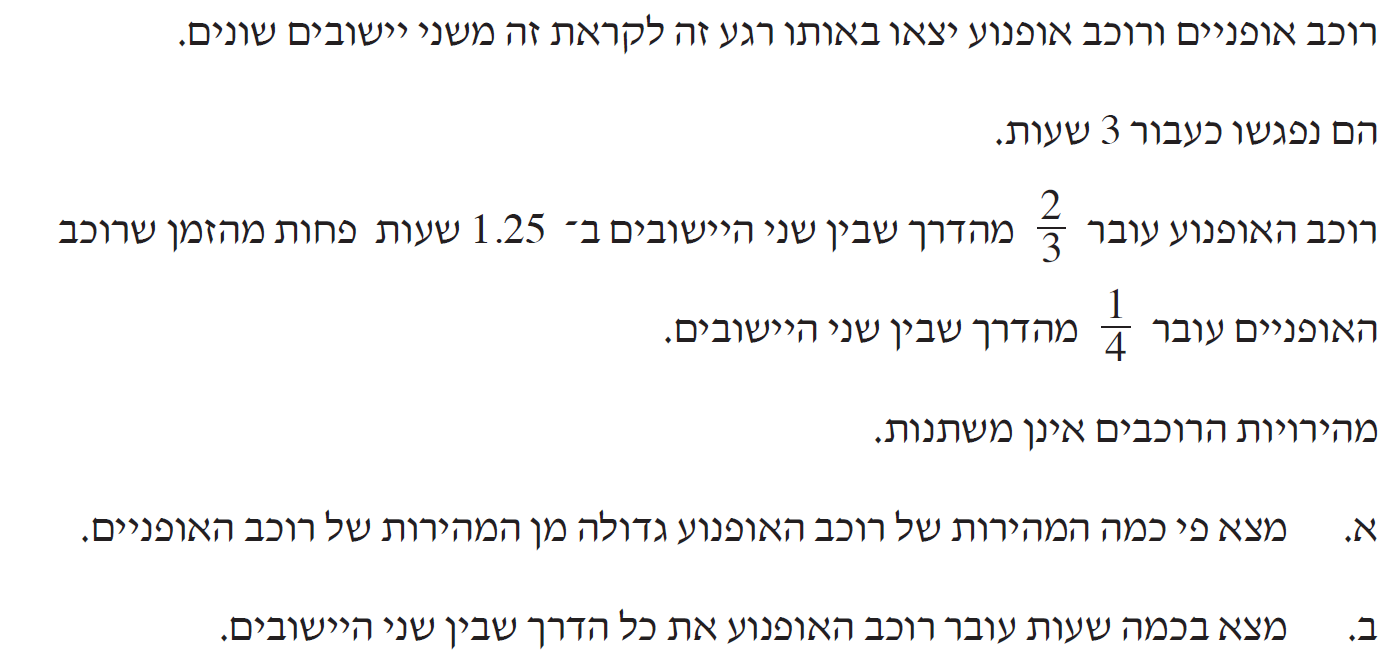
\includegraphics[width=.9\textwidth]{winter-2016-1}
\end{center}

\textbf{סעיף א}

\begin{center}
\selectlanguage{english}
\begin{tikzpicture}
\draw (0,0) node[left] {$A$} -- (10,0);
\draw (0,0) -- (0,6) node[left] {$B$};
\draw[dashed] (0,6) -- (10,6);
\draw[thick,name path=motor] (0,0) -- node[right,near start,xshift=1pt,yshift=-4pt] {
\R{אופנוע}
} (4,6);
\draw[thick,name path=bike] (0,6) -- node[above,near end,xshift=44pt,yshift=-10pt] {
\R{אופניים}
} (8,4);
\node at (8.4,3.7) {$\cdots$};
\path [name intersections={of=motor and bike,by=meeting}];
\coordinate (fourth) at (0,4.5);
\coordinate (two-thirds) at (0,3.5);
\path [name path=path-fourth] (fourth) -- +(6,0);
\path [name path=path-two-thirds] (two-thirds) -- +(6,0);
\path [name intersections={of=path-fourth and bike,by=meeting-fourth}];
\path [name intersections={of=path-two-thirds and motor,by=meeting-two-thirds}];
\draw[dashed] (meeting) |- coordinate (time) (0,0);
\draw[dashed] (meeting-fourth) -| coordinate (fourth-y) (0,0);
\draw[dashed] (meeting-fourth) |- coordinate (fourth-x) (0,0);
\draw[dashed] (meeting-two-thirds) -| coordinate (two-thirds-y) (0,0);
\draw[dashed] (meeting-two-thirds) |- coordinate (two-thirds-x) (0,0);
\fill (meeting) circle [radius=2pt];
\fill (time) circle [radius=2pt];
\fill (0,0) circle [radius=2pt];
\fill (two-thirds) circle [radius=2pt];
\fill (fourth) circle [radius=2pt];
\fill (fourth-x) circle [radius=2pt];
\fill (fourth-y) circle [radius=2pt];
\fill (meeting-fourth) circle [radius=2pt];
\fill (two-thirds-x) circle [radius=2pt];
\fill (two-thirds-y) circle [radius=2pt];
\fill (meeting-two-thirds) circle [radius=2pt];
\path (0,0) -- node[left] {$\frac{2}{3}x$} (two-thirds-y);
\path (0,6) -- node[left] {$\frac{1}{4}x$} (fourth-y);
\draw[<->] (0,-.5) -- node[fill=white] {$3$} (time |- 0,-.5);
\draw[<->] (fourth-x |- 0,-1) -- node[fill=white] {$5/4$} (two-thirds-x |- 0,-1);
\draw[<->] (0,-1.5) -- node[fill=white] {$T_m$} (two-thirds-x |- 0,-1.5);
\draw[<->] (0,-2) -- node[fill=white] {$T_b$} (fourth-x |- 0,-2);
\end{tikzpicture}
\end{center}

נסמן:
$=v_b$
מהירות אופניים,
$=v_m$
מהירות אופנוע,
$=x$
מרחק בין הערים,
$=T_m$
פרק הזמן שהאופנוע עובר
$\frac{2}{3}$
מהמרחק,
$=T_b$
פרק הזמן שהאופניים עובר
$\frac{1}{4}$
מהמרחק.

כאשר שני כלי הרכב נפגשים סכום המרחקים שהם עברו הוא המרחק בין הנקודות. המרחק לא נתון ולכן אנו משתמשים בנעלם
$x$:
\[
x = 3v_b + 3 v_m\,.
\]
הנתון השני הוא הקשר בין זמני הנסיעה של חלקי המרחק בין היישובים
$T_b=T_m+1.25$:
\[
\frac{x/4}{v_b} = \frac{2x/3}{v_m} + \frac{5}{4}\,.
\]
\np

נציב עבור
$x$,
נסמן את היחס בין המהירויות
$r=\disfrac{v_m}{v_b}$
ונקבל משוואה הריבועית:
\erh{14pt}
\begin{equationarray*}{rcl}
\frac{3v_b+3v_m}{4v_b}&=&\frac{2(3v_b+3v_m)}{3v_m}+\frac{5}{4}\\
\frac{3}{4}+\frac{3}{4}r&=&\frac{2}{r}+2+\frac{5}{4}\\
3r^2 - 10r - 8 &=& 0\,.
\end{equationarray*}
השורש החיובי הוא
$r=\disfrac{v_m}{v_b}=4$.


\textbf{סעיף ב}

נתונה משוואת המרחק בין היישובים:
\[
x = 3v_b + 3 v_m\,.
\]
נשתמש ביחס שחישבנו בסעיף א כדי לחשב את הזמן של נסיעת האופנוע:
\[
\frac{x}{v_m} = \frac{3v_b + 3 v_m}{v_m}=3\frac{v_b}{v_m}+3=\frac{3}{r}+3=\frac{3}{4}+3=\frac{15}{4}\quad \textrm{\R{שעות}}\,.
\]

%%%%%%%%%%%%%%%%%%%%%%%%%%%%%%%%%%%%%%%%%%%%%%%%%%%%%%%%%%%%%%%%

\np

\section{קיץ תשע"ה מועד ב}

\begin{center}
\selectlanguage{english}
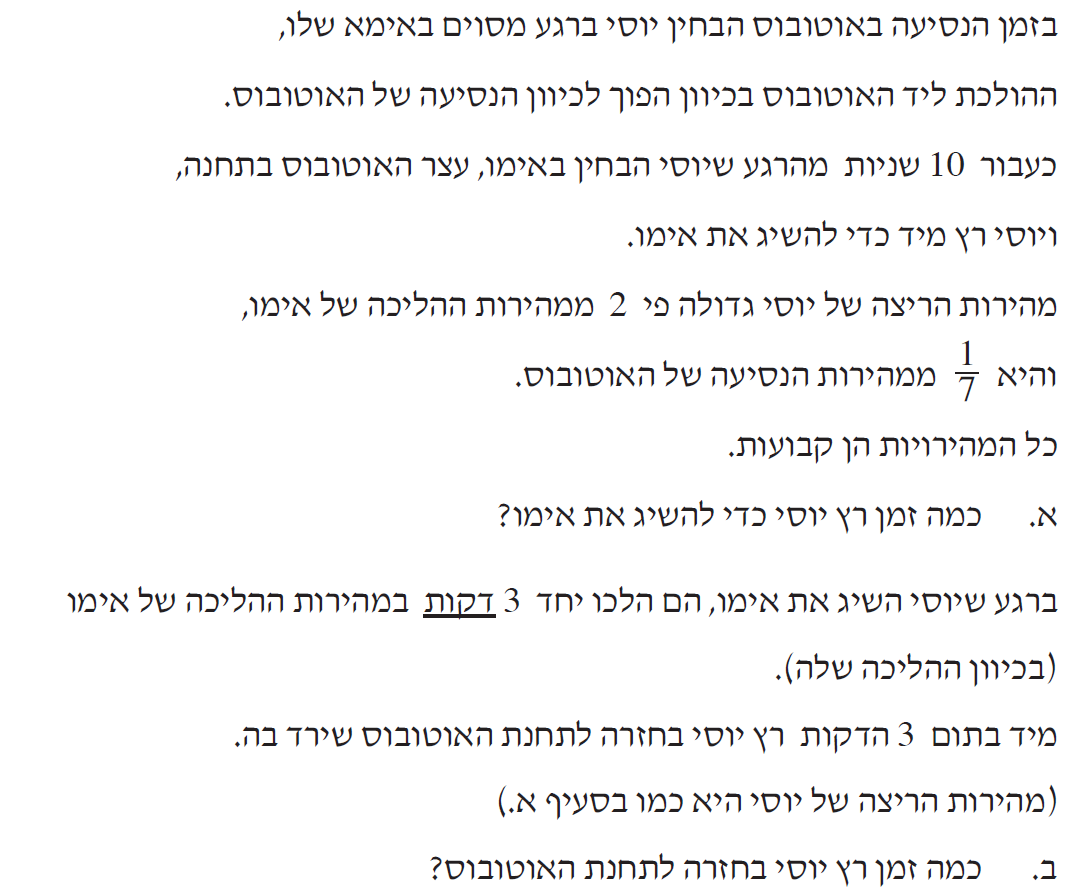
\includegraphics[width=.8\textwidth]{summer-2015b-1}
\end{center}

\vspace{-3ex}

\begin{center}
\selectlanguage{english}
\begin{tikzpicture}[scale=.85]
\draw (0,0) -- (14,0);
\draw (0,-4) node[left] {
\R{פרידה}
} -- (0,-2) node[left] {
\R{מפגש 2}
} -- (0,0) node[left] {
\R{מפגש 1}
} -- (0,4) node[left] {
\R{תחנה}
};
\fill (0,0) circle [radius=2pt];
\fill (1,0) circle [radius=2pt] node[below right] {$M$};
\fill (4,0) circle [radius=2pt] node[above] {$N$};
\fill (8,0) circle [radius=2pt] node[above] {$P$};
\fill (11,0) circle [radius=2pt] node[below right] {$Q$};
\fill (14,0) circle [radius=2pt] node[below] {$R$};
\draw[thick] (0,0) -- node[left] {$a$} (1,4) -- node[right,near start] {$b$} (4,-2);
\draw[thick] (0,0) -- node[below,near start,xshift=-2mm] {$c$} node[right,near end,yshift=2mm] {$d$} (8,-4)  node[below] {$P'$} -- (14,4)  node[right] {$R'$};
\draw[dashed] (0,4) -- (14,4);
\draw[dashed] (0,-2) -- (14,-2);
\draw[dashed] (0,-4) -- (14,-4);
\draw[dashed] (1,4)  node[above] {$M'$} -- (1,0);
\draw[dashed] (4,0) -- (4,-2) node[below,yshift=-1mm] {$N'$};
\draw[dashed] (8,-4) -- (8,0);
\draw[dashed] (11,0) -- (11,4);
\draw[dashed] (14,0) -- (14,4);
\draw[<->] (0,.7) -- node[fill=white] {$10$} (1,.7);
\draw[<->] (1,.7) -- node[near start,fill=white] {$t$} (4,.7);
\draw[<->] (4,.7) -- node[fill=white] {$180$} (8,.7);
\draw[<->] (8,.7) -- node[fill=white] {$t_1$} (11,.7);
\draw[<->] (11,.7) -- node[fill=white] {$t_2$} (14,.7);
\path (8,-2) --  node[below right,xshift=5mm,yshift=-2mm] {$e_1$} (11,0);
\path (11,0) --  node[left,yshift=3mm] {$e_2$} (14,4);
\end{tikzpicture}
\end{center}

\vspace{-3ex}

בתרשים סימנו את הקטעים:
\begin{center}
\begin{tabular}{rr}
\R{$=b$
יוסי רץ לפגישה עם אמא}
&
\R{$=a$
יוסי נוסע באוטובוס}\\
\R{$=d$
יוסי ואמא הולכים ביחד}
&
\R{$=c$
אמא הולכת עד למפגש עם יוסי}\\
&
\R{$=e_1+e_2$
יוסי רץ חזרה לתחנה}
\end{tabular}
\end{center}

\np

נסמן:
$=t$
הזמן שיוסי רץ מהתחנה כדי להשיג את אמא.

נסמן מהירויות:
$=v_y$
יוסי, 
$=v_a$
אמא, 
$=v_b$
אוטובוס.

נתון:
$v_y=2v_a$, $v_y=v_b/7$.

\medskip

\textbf{סעיף א}

את הזמן
$t$
נוכל לחשב ממשוואות התנועה מהמפגש הראשון )יוסי רואה את אימו( ועד למפגש השני )יוסי משיג את אימו(. המרחק מסומן
$NN'$
בתרשים. נוכל למצוא שתי משוואות עבור מרחק זה, אחד עבור אמא )קטע
$c$(:
\[
v_a(t+10),
\]
ואחד עבור יוסי )קטעים
$a,b$(:
\[
-v_b\cdot 10 + v_yt\,.
\]
שימו לב שבקטע 
$a$
יוסי 
\textbf{מתרחק}
מהמפגש ולכן המהירות שלילית.

נשווה את המרחקים ונציב את יחס המהירויות הנתון:
\erh{6pt}
\begin{equationarray*}{rcl}
 v_a(t+10)&=&v_yt -v_b\cdot 10\\
\frac{v_y}{2}(t+10)&=& v_yt - 7v_y 10\,.
\end{equationarray*}
הפתרון הוא
$150=t$
שניות.
\medskip

\textbf{סעיף ב}

מהתרשים קל לראות
\textbf{ששני}
קטעי הקווים
$e_1,e_2$
מתארים את הריצה של יוסי בחזרה לתחנה. רואים גם שהמרחק
$PP'$
של
$e_1$
הוא גם המרחק שאמא הולכת, קטעים 
$c,d$.
לפי התוצאה של סעיף א, לוקח לאמא
$10+150+180=340$
שניות לעבור מרחק זה. נתון שיוסי רץ פי שניים מהר יותר מההליכה של אמא, ולכן
$t_1=170$
שניות.

עבור הקטע השני
$e_2$,
המרחק
$RR'$
שווה למרחק
$MM'$,
המרחק שהאוטובוס עבר מהמפגש הראשון ועד התחנה. נתון שהאוטובוס עובר מרחק זה ב-%
$10$
שניות, ונתון שמהירות הריצה של יוסי פי שבע לאט ממהירות הנסיעה של האוטובוס, כך ש-%
$t_2=70$.

נסכם ונקבל שיוסי רץ מנקודת הפרידה לתחנה ב
$240=t_1+t_2$
שניות.

\bigskip

\textbf{שימו לב למלכודת:}
זמן ההליכה cיחד נתון בדקות ושאר הזמנים בשניות.

%%%%%%%%%%%%%%%%%%%%%%%%%%%%%%%%%%%%%%%%%%%%%%%%%%%%%%%%%%%%%%%%

\np

\section{קיץ תשע"ה מועד א}

\begin{center}
\selectlanguage{english}
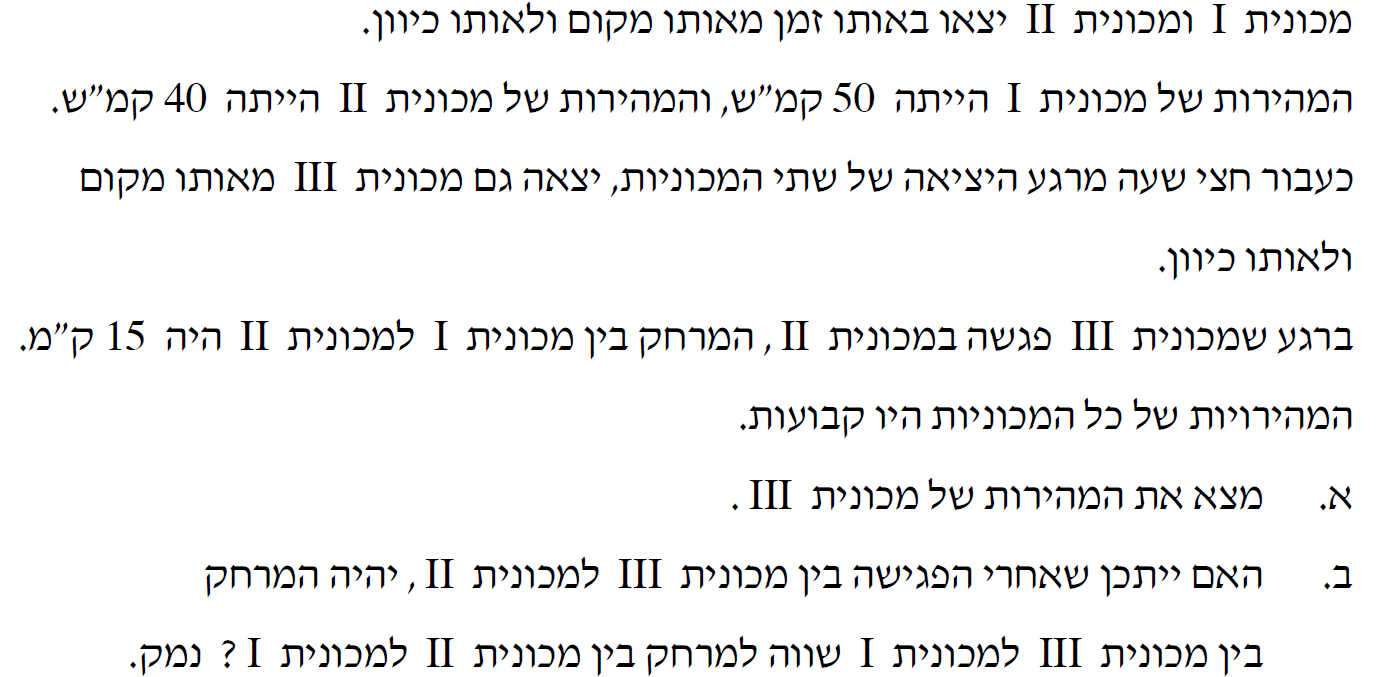
\includegraphics[width=.9\textwidth]{summer-2015a-1}
\end{center}

\begin{center}
\selectlanguage{english}
\begin{tikzpicture}[scale=1.2]
\draw (0,0) -- (10,0);
\draw (0,0) -- (0,6);
\draw[thick,name path=one] (0,0) -- node[below,near end,xshift=50pt,yshift=28pt] {I} (10,6);
\draw[thick,name path=two] (0,0) -- node[below,near end,xshift=50pt,yshift=14pt] {II} (10,3);
\draw[thick,name path=three] (3,0) -- node[above,near end,xshift=2pt,yshift=12pt] {III} (8,6);
\path [name intersections={of=one and three,by=one-three}];
\path [name intersections={of=two and three,by=two-three}];
\draw[dashed] (two-three) |- coordinate (time-two-three) (0,0);
\fill (0,0) circle [radius=2pt];
\fill (3,0) circle [radius=2pt];
\fill (one-three) circle [radius=2pt];
\fill (two-three) circle [radius=2pt];
\fill (time-two-three) circle [radius=2pt];
\node[above left] at (one-three) {$B$};
\node[below right] at (two-three) {$A$};
\path [name path=distance] (two-three) -| +(0,2);
\path [name intersections={of=one and distance,by=fifteen}];
\draw (two-three) -- (fifteen) node[above left] {
\R{ק"מ}
$15$};
\draw[->] (3.3,2.5) -- (3.8,1.7);
\fill (fifteen) circle [radius=2pt];
\draw[<->] (0,-.6) -- node[fill=white] {
\R{שעה}
 $1/2$} (3,-.6);
\draw[<->] (3,-.6) -- node[fill=white] {$t$} (time-two-three |- 0,-.6);
\end{tikzpicture}
\end{center}
המהירות של מכונית I גדולה מהמהירות של מכונית II, ולכן השיפוע שלו תלול יותר.

נסמן
$=t$
הזמן בין היציאה של III ועד למפגש שלו עם II,
$=v_3$
המהירות של III.

נתון: מהירות של I
$v_1=50$,
מהירות של II
$v_2=40$.

\textbf{סעיף א}

לאחר 
$t+1/2$
שעות, המכוניות II ו-III עברו אותו מרחק, ומכונית I עבר אותו מרחק ועוד 
$15$
ק"מ. נכתוב את משוואות התנועה לשני המקרים:
\begin{eqnarray*}
40(t+1/2) &=& v_3t\\
50(t+1/2) &=& v_3t + 15\,.
\end{eqnarray*}
מהמשוואות מתקבל
$t=1$
ואח"כ
$v_3=60$
קמ"ש.

\np

\textbf{סעיף ב}

נוסיף סימונים לתרשים שיעזרו לנו לפתור את הבעייה:

\begin{center}
\selectlanguage{english}
\begin{tikzpicture}[scale=1.2]
\draw (0,0) -- (10,0);
\draw (0,0) -- (0,6);
\draw[thick,name path=one] (0,0) -- node[below,near end,xshift=50pt,yshift=28pt] {I} (10,6);
\draw[thick,name path=two] (0,0) -- node[below,near end,xshift=50pt,yshift=14pt] {II} (10,3);
\draw[thick,name path=three] (3,0) -- node[above,near end,xshift=2pt,yshift=12pt] {III} (8,6);
\path [name intersections={of=one and three,by=one-three}];
\path [name intersections={of=two and three,by=two-three}];
\draw[dashed] (two-three) |- coordinate (time-two-three) (0,0);
\fill (0,0) circle [radius=2pt];
\fill (3,0) circle [radius=2pt];
\fill (one-three) circle [radius=2pt];
\fill (two-three) circle [radius=2pt];
\fill (time-two-three) circle [radius=2pt];
\node[above left] at (one-three) {$B$};
\node[below right] at (two-three) {$A$};
\path [name path=distance] (two-three) -| +(0,2);
\path [name intersections={of=one and distance,by=fifteen}];
\draw (two-three) -- (fifteen) node[above left] {
\R{ק"מ}
$15$};
\draw[->] (3.3,2.5) -- (3.8,1.7);
\fill (fifteen) circle [radius=2pt];
\draw[<->] (0,-.6) -- node[fill=white] {
\R{שעה}
 $1/2$} (3,-.6);
\draw[<->] (3,-.6) -- node[fill=white] {$t$} (time-two-three |- 0,-.6);
\draw[->] (4.5,3.2) -- +(.45,-.55);
\draw[<->,thick,densely dotted] (5.3,3.1) -- +(0,-1.5);
\draw[<->,thick,densely dotted] (5,2.95) -- +(0,-.5);
\node at (5.6,2.4) {I-II};
\node at (4.5,3.4) {I--III};
\draw[<->,thick,densely dotted] (7.8,4.6) -- node[right] {I--II} +(0,-2.2);
\draw[<->,thick,densely dotted] (7.8,4.8) -- node[right,yshift=3pt] {I--III} +(0,.8);
\end{tikzpicture}
\end{center}

נעיין בקווים מנוקדים בתרשים ונראה שהמרחקים לא יכולים שווים. בנקודה
$A$
הרחקים שווים, אבל מנקודה זו ועד לנקודה
$B$,
המרחק I--II גדל והמרחק I--III קטן.

בנקודה
$B$
המרחק I--II חיובי והמרחק I--III שווה לאפס. מכאן והלאה, שני המרחקים גדלים באותו קצב כי הפרשי המהירויות שווים:
$10=60-50=50-40$
קמ"ש.

\smallskip

\textbf{הוכחה בחישוב}

נסמן
$=t_A$
זמן מנקודה
$A$,
$=t_B$
זמן מנקודה
$B$,
$=d_B$
המרחק בין I ל-II בנקודה
$B$.

\smallskip

משמאל לנקודה
$B$
המרחקים שווים
\textbf{אם}:
\[
15 + (v_1-v_2)t_A \stackrel{?}{=} 15 + (v_1-v_3)t_A\,.
\]
נציב
$v_1=50, v_2=40, v_3=60$
ונקבל
$10=-10$,
כך הטיעון לא יכול להיות נכון.

\smallskip

מימין לנקודה
$B$
המרחקים שווים
\textbf{אם}:
\[
(v_3-v_1)t_B \stackrel{?}{=} d_B + (v_1-v_2)t_B\,.
\]
לאחר הצבה עבור המהירויות, נקבל שהטיעון נכון אם
$d_B=0$,
אבל אנחנו יודעים ש-%
$d_B > 15$.

%%%%%%%%%%%%%%%%%%%%%%%%%%%%%%%%%%%%%%%%%%%%%%%%%%%%%%%%%%%%%%%%

\np

\section{חורף תשע"ה}

\begin{center}
\selectlanguage{english}
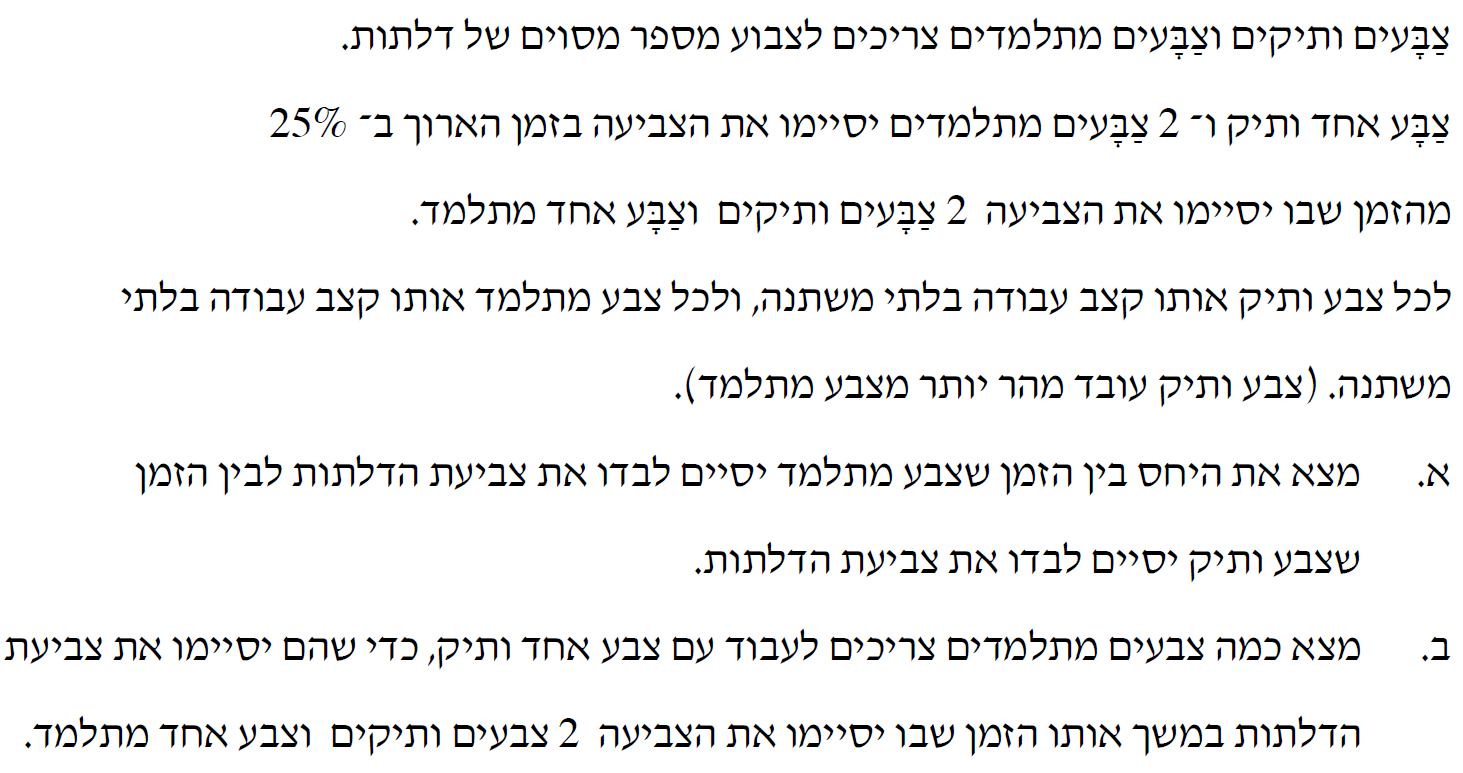
\includegraphics[width=\textwidth]{winter-2015-1}
\end{center}

\vspace{-2ex}

\textbf{סעיף א}

\begin{center}
\selectlanguage{english}
\begin{tikzpicture}
\draw (0,0) -- (10,0);
\draw (0,0) node[above left] {\R{אף דלת לא נצבע}}
-- (0,6) node[left] {\R{כל הדלתות נצבעו}};
\draw[dashed] (0,6) -- (10,6);
\draw[ultra thick] (0,0) -- node[left,near end,xshift=-2mm] {$2/t_v$} (8,4.5)  coordinate (two-one);
\draw[ultra thick] (0,4.5)  -- node[left,xshift=-2mm,yshift=2mm] {$1/t_m$} (8,6) coordinate (two-one-finish);
\draw[dotted,ultra thick] (0,4.5) -- (8,4.5);
\draw[thick] (0,0) -- node[left,yshift=2mm] {$1/t_v$} (10,2.25)  coordinate (one-two);
\draw[thick] (0,2.25)  -- node[left,near start,yshift=2mm] {$2/t_m$} (10,6) coordinate (one-two-finish);
\draw[dotted,thick] (0,2.25) -- (10,2.25);
\draw[dashed] (two-one-finish) -- (two-one-finish |- 0,0);
\draw[dashed] (one-two-finish) -- (one-two-finish |- 0,0);
\draw[<->] (0,-.6) -- node[fill=white] {$T$} (two-one-finish |- 0,-.6);
\draw[<->] (0,-1.2) -- node[fill=white] {$1.25 T$} (one-two-finish |- 0,-1.2);
\end{tikzpicture}
\end{center}
\vspace{-1ex}

נסמן את הזמנים לצביעת כל הדלתות: 
$=t_v$
צבע ותיק,
$=t_m$
צבע מתלמד.

השאלה שואלת על יחס בין זמנים, ולכן אין חשיבות לזמן הכולל לצביעות כל הדלתות. 
נסמן
$=1$
הזמן הכולל של שני ותיקים ומתלמד אחד, ו-%
$=1.25$
הזמן הכולל של שני מתלמדים וותיק אחד.

\smallskip

\noindent\textbf{הסבר על התרשים}

הצבעים עובדים במקביל אבל הציר בתרשים מראה
\textbf{חלוקת העבודה},
כאילו שצבע )או זוג צבעים( מסיים את חלקו בעבודה ואחר כך הצבע )או הזוג( השני מתחיל את חלקו. כאשר יש זוג צבעים הם רשומים כצבע אחד עם הספק כפול. הקווים הדקים מראים צבע אחד ותיק 
$(1/t_v)$
ושני צבעים מתלמדים
$(2/t_m)$.
הקווים העבים מראים שני צבעים ותיקים
$(2/t_v)$
וצבע אחד מתלמד
$(1/t_m)$.

\np

שני ההרכבים סיימו את כל העבודה, ומכאן שמשוואות ההספק נותנות אותו ערך:
\[
\frac{2}{t_v}\cdot 1 \:+\: \frac{1}{t_m}\cdot 1 \;=\; \frac{1}{t_v}\cdot 1.25 \:+\: \frac{2}{t_m} \cdot 1.25 \,.
\]
הפתרון הוא:
\[
\frac{t_m}{t_v}=2\,.
\]

\textbf{סעיף ב}

\begin{center}
\selectlanguage{english}
\begin{tikzpicture}
\draw (0,0) -- (10,0);
\draw (0,0) node[above left] {\R{אף דלת לא נצבע}}
-- (0,6) node[left] {\R{כל הדלתות נצבעו}};
\draw[dashed] (0,6) -- (10,6);
\draw[ultra thick] (0,0) -- node[left,near end,xshift=-2mm] {$2/t_v$} (8,4.5)  coordinate (two-one);
\draw[ultra thick] (0,4.5)  -- node[left,xshift=-2mm,yshift=2mm] {$1/t_m$} (8,6) coordinate (two-one-finish);
\draw[dashed,ultra thick] (0,4.5) -- (8,4.5);
\draw[thick] (0,0) -- node[left,yshift=2mm] {$1/t_v$} (8,2.25)  coordinate (one-two);
\draw[thick] (0,2.25)  -- node[left,near start,yshift=2mm] {$n/t_m$} (8,6) coordinate (one-two-finish);
\draw[dashed,blue] (0,2.25) -- (8,2.25);
\draw[dashed] (two-one-finish) -- (two-one-finish |- 0,0);
\draw[<->] (0,-.6) -- node[fill=white] {$1$} (two-one-finish |- 0,-.6);
\end{tikzpicture}
\end{center}

נסמן
$=n$
מספר הבצעים המתלמדים. העבודה של שני ההרכבים שווה ולכן:
\[
\frac{2}{t_v} + \frac{1}{t_m} = \frac{1}{t_v} + \frac{n}{t_m}\,.
\]
נשתמש ביחס שחישבנו בסעיף א ונקבל:
\[
n = \frac{t_m}{t_v}+1 = 2+1=3\,.
\]

%%%%%%%%%%%%%%%%%%%%%%%%%%%%%%%%%%%%%%%%%%%%%%%%%%%%%%%%%%%%%%%%

\np

\section{קיץ תשע"ד מועד ב}

\begin{center}
\selectlanguage{english}
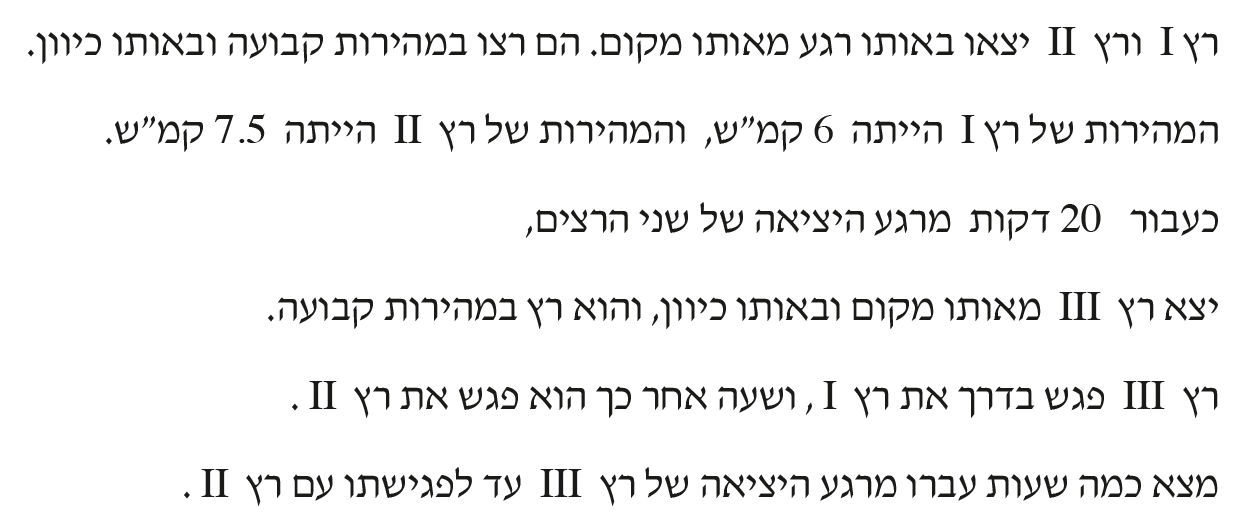
\includegraphics[width=.9\textwidth]{summer-2014b-1}
\end{center}

\begin{center}
\selectlanguage{english}
\begin{tikzpicture}
\draw (0,0) -- (10,0);
\draw (0,0) -- (0,6);
\draw[thick,name path=one] (0,0) -- node[below,near end,xshift=4pt] {I} (10,4);
\draw[thick,name path=two] (0,0) -- node[below,near end,xshift=16pt,yshift=6pt] {II} (10,6);
\draw[thick,name path=three] (2,0) -- node[above,near end,yshift=6pt] {III} (9,6);
\path [name intersections={of=one and three,by=one-three}];
\path [name intersections={of=two and three,by=two-three}];
\draw[dashed] (one-three) |- coordinate (time-one-three) (0,0);
\draw[dashed] (two-three) |- coordinate (time-two-three) (0,0);
\fill (0,0) circle [radius=2pt];
\fill (2,0) circle [radius=2pt];
\fill (one-three) circle [radius=2pt];
\fill (two-three) circle [radius=2pt];
\fill (time-one-three) circle [radius=2pt];
\fill (time-two-three) circle [radius=2pt];
\draw[<->] (0,-.6) -- node[fill=white] {
\R{שעה}
 $1/3$} (2,-.6);
\draw[<->] (2,-.6) -- node[fill=white] {$t$} (time-one-three |- 0,-.6);
\draw[<->] (time-one-three |- 0,-.6) -- node[fill=white] {
\R{שעה}
 $1$} (time-two-three |- 0,-.6);
\end{tikzpicture}
\end{center}

נסמן:
$=t$
הזמן בין היציאה של III ועד למפגש עם I,
$=v$
המהירות של III.

נתון:
$=6$
מהירות של I ו-
$=7.5$
המהירות של II. שימו לב לשיפועים של הקווים.

בכל מפגש בין שתי דמויות המרחקים שעברו שווים. המפגש בין I ל-III:
\[
6(t+1/3) = vt\,,
\]
והמפגש בין II ו-III:
\[
7.5(1/3+t+1) = v(t+1)\,.
\]
מהמשוואה הראשונה נקבל ביטוי עבור 
$v$
ונציב במשוואה השנייה. נקבל משוואה ריבועית ב-%
$t$:
\[
1.5t^2 + 2t - 2 = 0\,,
\]
שיש לה פתרון חיובי אחד
$t=2/3$.

\smallskip

הזמן מהיציאה של III ועד המפגש עם II הוא
$t+1=5/3$
שעות.

%%%%%%%%%%%%%%%%%%%%%%%%%%%%%%%%%%%%%%%%%%%%%%%%%%%%%%%%%%%%%%%%

\np

\section{קיץ תשע"ד מועד א}

\begin{center}
\selectlanguage{english}
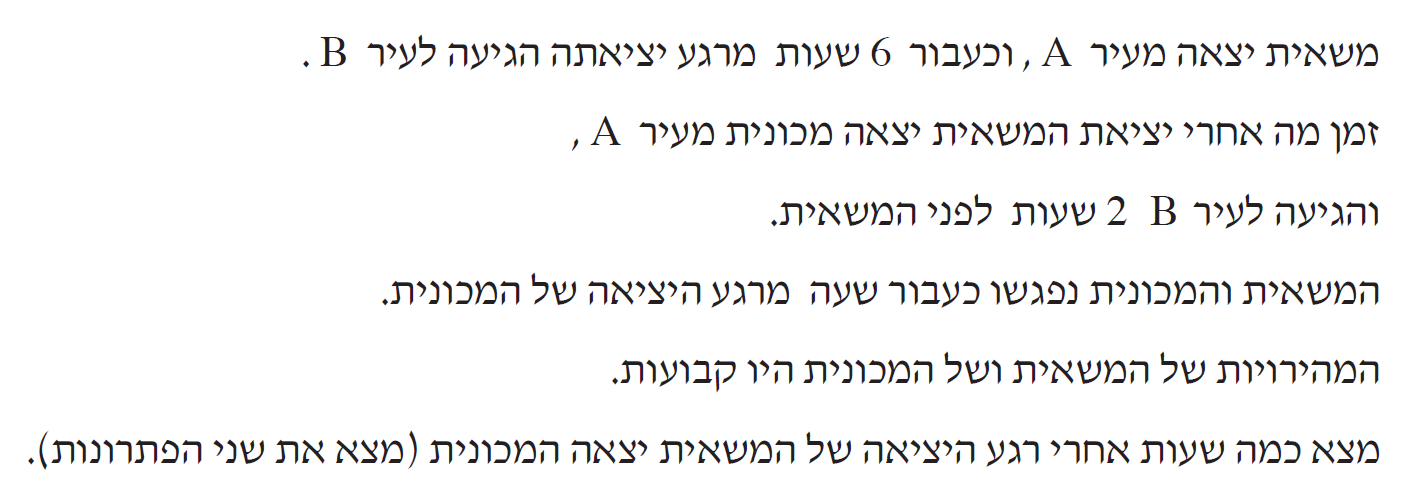
\includegraphics[width=\textwidth]{summer-2014a-1}
\end{center}

\begin{center}
\selectlanguage{english}
\begin{tikzpicture}
\draw (0,0) node[left] {$A$} -- (10,0);
\draw (0,0) -- (0,6) node[left] {$B$};
\draw[dashed] (0,6) -- (10,6);
\draw[thick,name path=truck] (0,0) -- node[left,near start,xshift=-6pt] {
\R{משאית}
} (10,6);
\draw[thick,name path=car] (3,0) -- node[left,near end] {
\R{מכונית}
} (7,6);
\path [name intersections={of=truck and car,by=meeting}];
\draw[dashed] (meeting) |- coordinate (time) (0,0);
\draw[dashed] (10,0) -- (10,6);
\draw[dashed] (7,0) -- (7,6);
\fill (meeting) circle [radius=2pt];
\fill (time) circle [radius=2pt];
\fill (0,0) circle [radius=2pt];
\fill (3,0) circle [radius=2pt];
\fill (7,0) circle [radius=2pt];
\fill (10,0) circle [radius=2pt];
\draw[<->] (0,-.5) -- node[fill=white] {$t$} (3,-.5);
\draw[<->] (3,-.5) -- node[fill=white] {
\R{שעה}
 $1$} (time |- 0,-.5);
\draw[<->] (time |- 0,-.5) -- node[fill=white] {$3-t$} (7,-.5);
\draw[<->] (7,-.5) -- node[fill=white] {
\R{שעות}
 $2$} (10,-.5);
\draw[<->] (3.1,-1.2) -- node[fill=white] {$4-t$} (6.9,-1.2);
\draw[<->] (0,-1.8) -- node[fill=white] {
\R{שעות}
 $6$} (10,-1.8);
\end{tikzpicture}
\end{center}

המפתח לפתרון הוא לסמן כל פרק זמן כפי שעשינו בתרשים.

נסמן:
$=t$
זמן יציאת המכונית,
$=v_c$
מהירות המכונית,
$=v_m$
מהירות המשאית.

\smallskip

נכתוב משוואות למרחקים שווים, מ-
$A$
עד למפגש ומ-
$A$
עד ל-
$B$:
\begin{eqnarray*}
v_m(t+1) &=& v_c\cdot 1\\
v_m \cdot 6 &=& v_c (4-t)\,.
\end{eqnarray*}
משתי המשוואות מתקבלת משוואה ריבועית ב-
$t$:
\[
t^2 - 3t + 2 = 0
\]
שיש לה שני פתרונות
$t=1$
שעה ו-
$t=2$
שעות.

%%%%%%%%%%%%%%%%%%%%%%%%%%%%%%%%%%%%%%%%%%%%%%%%%%%%%%%%%%%%%%%%

\np

\section{חורף תשע"ד}

\begin{center}
\selectlanguage{english}
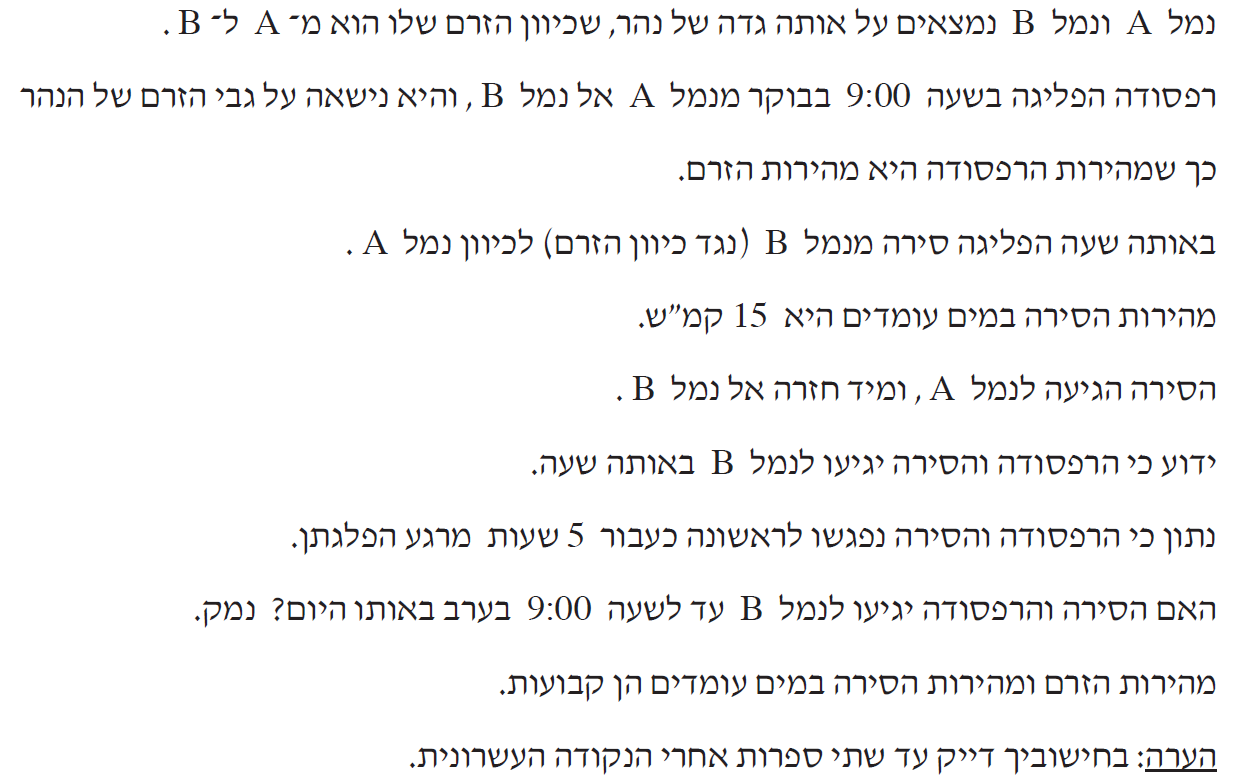
\includegraphics[width=\textwidth]{winter-2014-1}
\end{center}

\begin{center}
\selectlanguage{english}
\begin{tikzpicture}
\draw (0,0) node[below left] {$A$} node[below,xshift=-14pt,yshift=-10pt] {\p{9:00}} -- (10,0);
\draw (0,0) -- (0,6) node[above left] {$B$};
\draw[dashed] (0,6) -- (10,6);
\draw[thick,name path=raft] (0,0) -- node[left,near start,xshift=-4pt] {
\R{רפסודה}
} (10,6);
\draw[thick,name path=boat] (0,6) -- node[right,near start,xshift=2pt] {
\R{סירה}
} (8,0) -- (10,6);
\path [name intersections={of=boat and raft,by=meeting}];
\draw[dashed] (meeting) |- coordinate (time) (0,0);
\draw[dashed] (meeting) -| coordinate (distance) (0,0);
\draw[dashed] (8,0) -- (8,6);
\draw[dashed] (10,0) -- (10,6);
\fill (meeting) circle [radius=2pt];
\fill (time) circle [radius=2pt];
\fill (0,0) circle [radius=2pt];
\fill (8,0) circle [radius=2pt];
\fill (8,6) circle [radius=2pt];
\fill (10,6) circle [radius=2pt];
\fill (10,0) circle [radius=2pt];
\fill (distance) circle [radius=2pt];
\draw[<->] (-.4,0) -- node[fill=white] {$d_1$} (distance -| -.4,0);
\draw[<->] (distance -| -.4,0) -- node[fill=white] {$d_2$} (-.4,6);
\draw[<->] (-.9,0) -- node[fill=white] {$d$} (-.9,6);
\draw[<->] (0,-.6) -- node[above] {
\R{שעות}
 $5$} (time |- 0,-.6);
\draw[<->] (0,-1.2) -- node[fill=white] {$t_1$} (8,-1.2);
\draw[<->] (8,-1.2) -- node[fill=white] {$t_2$} (10,-1.2);
\draw[<->] (0,-1.8) -- node[fill=white] {$t$} (10,-1.8);
\end{tikzpicture}
\end{center}

\vspace{-2ex}

נסמן:
$=d$
מרחק בין שני הנמלים,
$=d_1$
מרחק בין
$A$
למפגש,
$=d_2$
מרחק בין 
$B$
למפגש.

$=t$
זמן עד למפגש ב-%
$B$,
$=v$
מהירות הזרם.

\smallskip

כאשר הסירה מפליגה מ-%
$B$
ל-%
$A$
ובחזרה ל-%
$B$,
היא עוברת מרחק כפול מהמרחק שהרפסודה עוברת באותו פרק זמן. נשווה את משוואות התנועה:

\np

\[
\frac{d}{v} = \frac{d}{15-v} + \frac{d}{15+v}\,.
\]
$d$
מצטמצם ונקבל משוואה ריבועית במהירות הזרם
$v$:
\[
v^2+30v-225=0\,.
\]
השורש החיובי שלה הוא
$v=6.21$.

\smallskip

עכשיו שאנחנו יודעים את המהירויות, והזמן עד למפגש נתון, ננסה לחשב את המרחק 
$d$,
שהוא הסכום של המרחקים שעוברים הרפסודה והסירה:
\[
d = 5v + 5(15-v)\,.
\]
הפתרון הוא
$d=75$
)ללא תלות במהירות הזרם
$v$(.

\smallskip

את הזמן עד המפגש בנמל 
$B$
אפשר לחשב לפי ההפלגה של הסירה או לפי ההפלגה של הרפסודה. כמובן שפשוט יותר לחשב עבור הקטע היחיד של הרפסודה:
\[
t = \frac{d}{v} = \frac{75}{6.21} \approx 12.08\,.
\]
בכל זאת נבדוק לפי הסירה:
\[
t = \frac{d}{15-v} + \frac{d}{15+v} = \frac{75}{8.79} + \frac{75}{21.21}= 8.532 + 3.536 \approx 12.07\,.
\]
בגלל עיגול של החישובים יש הבדל קטן בין שתי התוצאות.

הסירה והרפסודה יצאו בשעה
\L{\p{09:00}}
בבוקר וההפלגות לקחו יותר מ-%
$12$
שעות, כך המפגש השני התקיים לאחר השעה
\L{\p{09:00}}
בערב.


%%%%%%%%%%%%%%%%%%%%%%%%%%%%%%%%%%%%%%%%%%%%%%%%%%%%%%%%%%%%%%%%

\selectlanguage{english}
\clearpage
\selectlanguage{hebrew}


\section*{המלצות: תנועה והספק}

\addcontentsline{cot}{chapter}{המלצות: תנועה והספק}

\begin{itemize}

\item
בניגוד תרשימים חד-ממדיים האורך של קטע קו הוא מרחק הנסיעה, כאן מרחק הנסיעה הוא ההפרש בציר האנכי בין הנקודה ההתחלתית לנקודה הסופית. קטע הקו עצמו יהיה משופע ולכן יהיה אורך יותר ממרחק הנסיעה.

\item
הקושי בפתרון של הבעיות הללו נובע מהצורך לתרגם את התיאורים המילוליים למשוואת. אפשר בקלות להתבלבל כאשר מתרגמים ביטויים כגון "לפני", "אחרי", "מהר יותר", "לאט יותר".  בתרשים קל ליצג את התיאורים הללו: נקודות שהן "לפני" ו-"אחרי" נקודת ייחוס יוצגו שמאלה או ימינה מנקודת הייחוס בציר הזמן. קו המסמן מסלול "מהר יותר" יוצג עם שיפוע תלול יותר מקו המסמן מסלול "לאט יותר".

\item
מומלץ להכין תרשימים גדולים וברורים כדי שהסימנים שמוסיפים ממידע נתון או ממידע המתקבל מחישובים יהיו קריאים. לעתים, כדאי להכין תרשימים חדשים לכל סעיף כדי שמידע הנחוץ רק לסעיף אחד לא יקשה על עיון במידע הנחוץ לסעיף אחר.

\item
מצאתי שאפשר "לקרוא" את המשוואות ישירות מהתרשימים. לחילופין אפשר גם לסדר את הנתונים בטבלה כמקובל.

\item 
נקודות מפגש נוחות מאוד לכתיבת זוג משוואות תנועה עם אותם נעלמים. הזמנים האם אותם זמנים )לפעמים בתוספת קבוע(, והמרחקים שווים )אם הדמויות נוסעות בותו כיוון(, או שסכום המרחקים שווה למרחק בין נקודות הקצה )כאשר הדמויות נוסעות אחת כלפי השנייה(.

\item 
פתרון המשוואות עצמן הוא בדרך כלל קל: שני משוואות עם שני נעלמים, כאשר המשוואות שיש לפתור הן לינאריות או ריבועיות.

\end{itemize}

\npchap


\tikzsetfigurename{series}
% !TeX root = bagrut-all.tex

\selectlanguage{hebrew}

\chapter{סדרות}


%%%%%%%%%%%%%%%%%%%%%%%%%%%%%%%%%%%%%%%%%%%%%%%%%%%%%%%%%%%%%%%%%%%

\section{קיץ תשע"ח מועד ב}

\begin{center}
\selectlanguage{english}
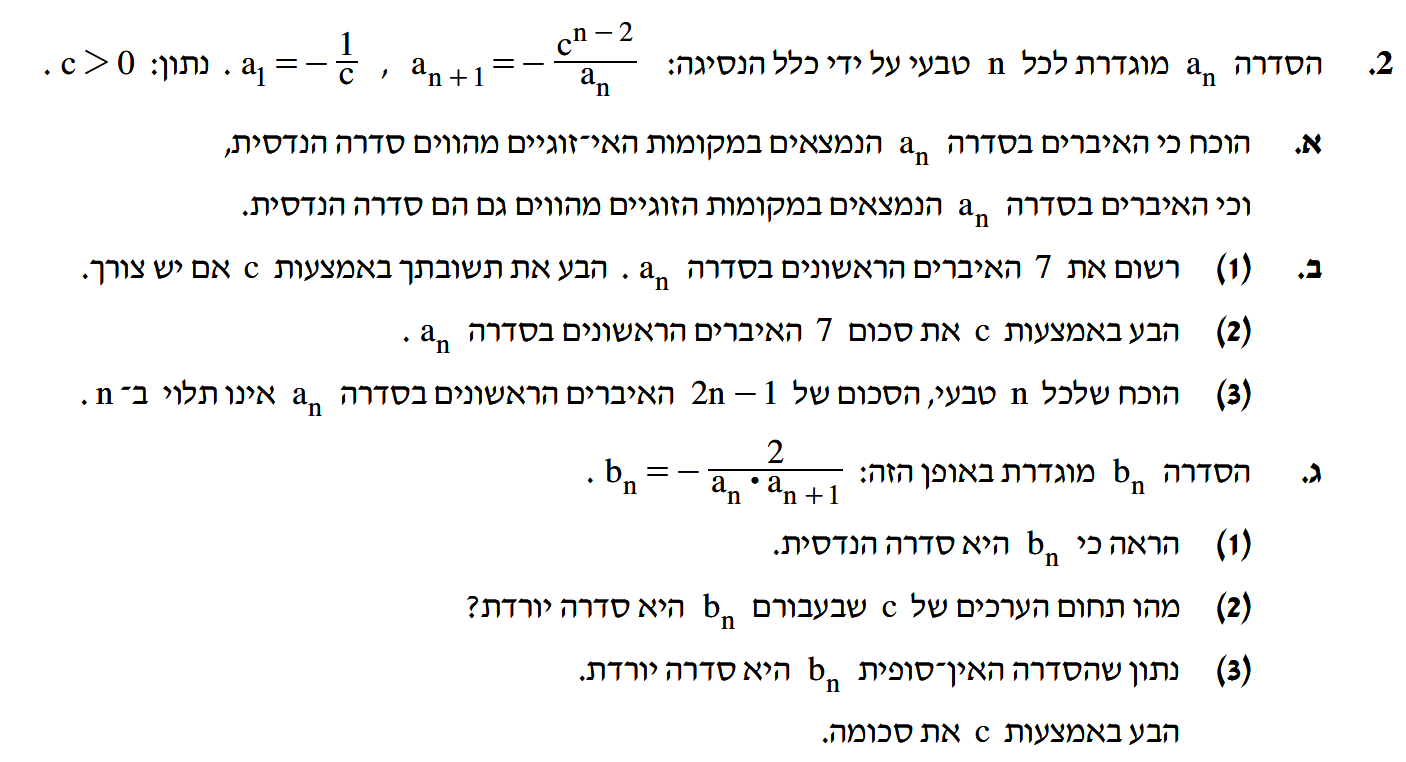
\includegraphics[width=\textwidth]{summer-2018b-2}
\end{center}
\vspace{-1ex}

\textbf{סעיף א}

כדי להוכיח שסדרה המוגדרת על ידי כלל נסיגה היא הנדסית, לא כדאי לחשב מנה של שני איברים עוקבים, כי איברים לא יצטמצמו. במקום זה, יש להציב בתוך כלל הנסיגה כדי לקבל ערך של איבר כתלות של איבר אחר:
\[
a_{n+1} = -\frac{c^{n-2}}{a_n} = -\frac{c^{n-2}}{\displaystyle -\frac{c^{n-3}}{a_{n-1}}} = ca_{n-1}\,.
\]
המנה
$a_{n+1}/a_{n-1}=c$
קבועה ולא תלוי ב-%
$n$.
ההוכחה נכונה עבור כל זוג של איברים שיש הפרש של שניים במקומות בסדרה, ולכן ההוכחה נכונה גם עבור מספרים זוגיים וגם עבור מספרים א-זוגיים.

\smallskip

\textbf{סעיף ב}
$(1)$

הסדרות של הזוגיים והאי-זוגיים הן סדרות הנדסיות
\textbf{נפרדות}
ויש לחשב את האיברים בנפרד:

\vspace{-2ex}

\[
\erh{12pt}
\begin{array}{l}
a_1=-\displaystyle\frac{1}{c},\;\;a_3=ca_1=-1,\;\;a_5=ca_3=-c,\;\;a_7=ca_5=-c^2\\
a_2=\displaystyle
-\frac{c^{1-2}}{a_1}=
-\frac{c^{-1}}{-\frac{1}{c}}=1,\;\;a_4=ca_2=c,\;\;a_6=ca_4=c^2\,.
\end{array}
\]
שבעת האיברים הראשונים של הסדרה הם:
\[
-\frac{1}{c}\,,1\,, -1\,, c\,, -c\,, c^2\,, -c^2\,.
\]

\np

\textbf{סעיף ב}
$(2)$

כאשר מסכמים את האיברים הם מצטמצמים פרט לאיבר הראשון, ולכן
$S_7=-\frac{1}{c}$.

\smallskip

\textbf{סעיף ב}
$(3)$

כאשר יש מספר אי-זוגי של איברים המתחילים ממקום אי-זוגי, מספר האיברים האי-זוגיים גדול באחד ממספר האיברים הזוגיים. נבדוק דוגמה:
\[
a_1\,,a_2\,,a_3\,,a_4\,,a_5\,,a_6\,,a_7\,,a_8\,,a_9\,.
\]
מספר האיברים הוא
$9$,
מהם
$5$
אי-זוגיים ו-%
$4$
זוגיים.

נצטרך לסכם את זוגיים והאי-זוגיים בנפרד, כי הסדרה המקורית אינה הנדסית. עבור שתי התת-סדרות, המנה הוא 
$c$,
אבל האיבר הראשון שונה 
$-\frac{1}{c}, 1$:
\[
S_{\mathit{odd}}+S_{\mathit{even}}=-\frac{1}{c}\frac{c^n-1}{c-1}+ 1\cdot\frac{c^{n-1}-1}{c-1}=
%\frac{-c^{n-1}+c^{-1} + c^{n-1}-1}{c-1}=
-\frac{1}{c}\,,
\]
לא תלוי ב-%
$n$.

\smallskip

\textbf{סעיף ג}
$(1)$

כאן הסדרה נתונה על ידי נוסחה ולא כלל נסיגה, ולכן ניתן לחשב ישירות את המנה:
\[
\frac{b_{n+1}}{b_n} = \frac{\displaystyle\frac{2}{a_{n+1}a_{n+2}}}{\displaystyle\frac{2}{a_{n}a_{n+1}}}= \frac{\displaystyle \frac{1}{a_{n+2}}}{\displaystyle \frac{1}{a_{n}}} =  \frac{1}{\displaystyle\frac{a_{n+2}}{a_n}} = \frac{1}{c}\,.
\]
\textbf{סעיף ג}
$(2)$

סדרה יורדת אם
$0<q=\displaystyle\frac{1}{c} < 1$.
נתון
$c>0$,
ולכן הסדרה יורדת כאשר
$c>1$.

\smallskip

\textbf{סעיף ג}
$(3)$

עבור סדרה הנדסית יורדת:
\erh{14pt}
\begin{equationarray*}{rcl}
S_b&=&\displaystyle\frac{b_1}{1-(1/c)}\\
&=&\frac{-2}{a_1\cdot a_{2}}\cdot \frac{c}{c-1}\\
&=&\frac{-2}{\displaystyle-\frac{1}{c}\cdot  1}\cdot \frac{c}{c-1}
=\frac{2c^2}{c-1}\,.
\end{equationarray*}

%%%%%%%%%%%%%%%%%%%%%%%%%%%%%%%%%%%%%%%%%%%%%%%%%%%%%%%%%%%%%%%%%%%
\np
\section{קיץ תשע"ח מועד א}

\begin{center}
\selectlanguage{english}
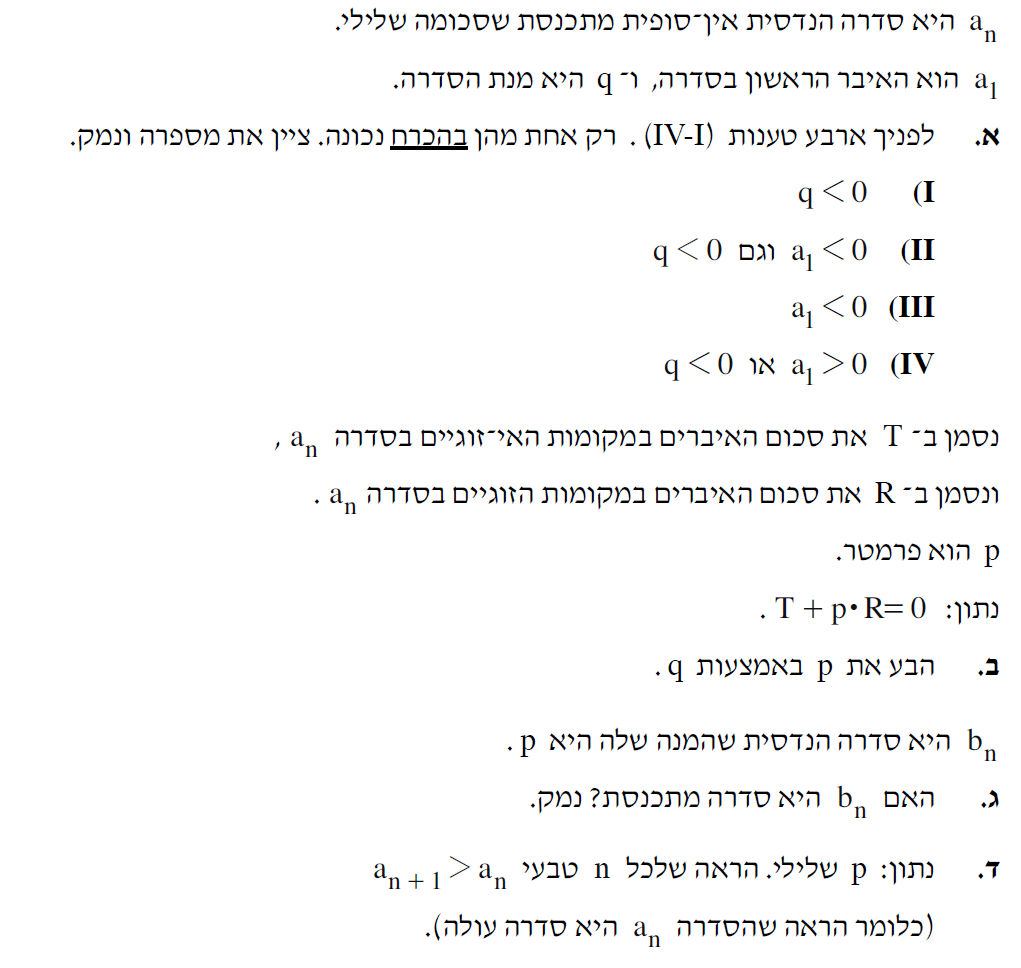
\includegraphics[width=.95\textwidth]{summer-2018a-2}
\end{center}

\textbf{סעיף א}

השאלה יפה כי היא דורשת חשיבה, לא חישובים! נבדוק את הטענות על סדרה מוכרת:
\[
1+ \frac{1}{2} + \frac{1}{4} + \frac{1}{8} + \cdots = 2\,.
\]
אם נהפוך את כל הסימנים למינוס, נקבל סדרה שסכומה שלילי:
\[
-1 - \frac{1}{2} - \frac{1}{4} - \frac{1}{8} - \cdots = -\left(1+ \frac{1}{2} + \frac{1}{4} + \frac{1}{8} + \cdots\right) = -2\,.
\]
ברור שהמנה עדיין חיובית:
\[
\frac{-2^{-(n+1)}}{-2^{-n}}=2^{-1}=\frac{1}{2}\,.
\]
נעבור לסדרה כללית. סדרה הנדסית מתכנסת רק אם
$|q|<1$.
מהנוסחה עבור הסכום:
\[
S = \frac{a_1}{1-q} <0\,,
\]

\np

ניתן לראות ש-% 
$a_1$
חייב להיות שלילי כי המכנה חיובי
$0 < 1-q < 2$.

אפשר לפסול מייד תשובות 
\L{I, II, IV}
ונשאר רק תשובה
\L{III}.

\smallskip

\textbf{סעיף ב}

שני תת-הסדרות הן הנדסית עם מנה זהה
$q^2$.
האיברים הראשונים הם
$a_1$
עבור האי-זוגיים ו-%
$a_2=a_1q$
עבור הזוגיים. הסכומים הם:
\[
T = \frac{a_1}{1-q^2},\quad\quad R = \frac{a_1q}{1-q^2}\,.
\]
מהמשוואה הנתונה
$T+pR=0$,
נקבל
$\quad 1+pq=0\quad$
ו-%
$p=-\displaystyle\frac{1}{q}\quad$.

\smallskip

\textbf{סעיף ג}

הסדרה לא מתכנסת כי 
$|q|<1$
גורר
$|p|>1$.

\smallskip

\textbf{סעיף ד}

שימו לב שהשאלה שואלת על
\textbf{הסדרה המקורית}
$a_n$
ולא על 
$b_n$!
נתון ש-%
$p$
שלילי ולכן
$q=-\displaystyle\frac{1}{p}$
חיובי. נתון שהסדרה מתכנסת ולכן
$0<q<1$,
חיובי. מצאנו בסעיף א ש-%
$a_1$
שלילי. מכפלה של מספר שלילי
$x$
עם מספר חיובי פחות מ-%
$1$
מקטינה את הערך המוחלט
$|x|$
שלו. ככל השערך המחולט של מספר שליליים קטן, הערך שלו עולה. לכן,
$a_{n+1}>a_n$.

נבדוק בדוגמה: אם 
$a_n=-6,q=\frac{1}{2}$,
אז:
\[
a_{n+1} = a_nq = -6\cdot \frac{1}{2} = -3 \;> \; -6 =a_n\,.
\]


%%%%%%%%%%%%%%%%%%%%%%%%%%%%%%%%%%%%%%%%%%%%%%%%%%%%%%%%%%%%%%%%%%%

\np
\section{חורף תשע"ח}

\begin{center}
\selectlanguage{english}
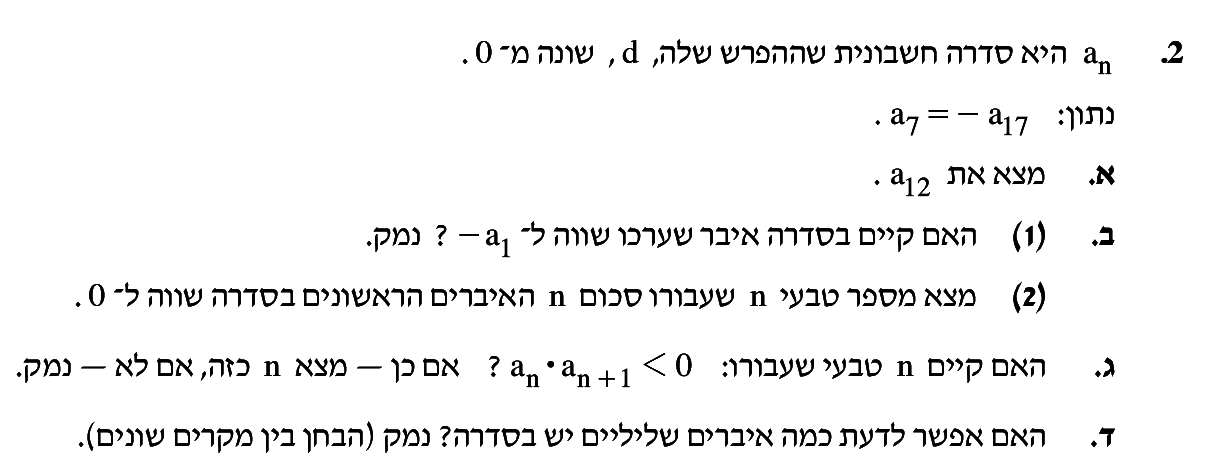
\includegraphics[width=.95\textwidth]{winter-2018-2}
\end{center}

\vspace{-1ex}

שאלה זו מתאפיין בהצבה של נוסחאות לאיברים מסויימים לתוך הנוסחאות הכלליות.

\smallskip

\textbf{סעיף א}

נציב 
$n=7, n=17$
במשוואה לאיבר ה-%
$n$:
\[
\erh{2pt}
\begin{array}{l}
a_7=a_1+(7-1)d = -(a_1+(17-1)d)=-a_{17}\\
a_1+11d=0\\
a_{12}=a_1+11d=0\,.
\end{array}
\]
\textbf{סעיף ב}
$(1)$

נשווה את
$-a_1$
לנוסחה לאיבר כללי:
\[
-a_1 = a_n = a_1 + (n-1)d\,.
\]
נציב
$a_1=-11d$
שישבנו בסעיף א:
\[
-(-11d) = -11d + (n-1)d\,.
\]
$d$
מצטמצם ונקבל
$n=23$.

\smallskip

\textbf{סעיף ב}
$(2)$

נציב
$a_1=-11d$
 בנוסחה לסכום של סדרה חשבונית:
\[
\frac{n}{2}(2a_1+(n-1)d) = \frac{n}{2}(2\cdot -11d+(n-1)d) =\frac{dn}{2} (n-23)=0\,.
\]
נתון שההפרש 
$d$
שונה מאפס וש-%
$n$
מספר טבעי ולכן חיובי, כך שהביטוי מתאפס רק עבור
$n=23$.

\np

\textbf{סעיף ג}

אם איבר חיובי וההפרש חיובי, המכפלה של שני איברים עוקבים היא חיובית, וכך גם אם שניהם שליליים. האפשרות היחידה לקבל מכפלה שלילית היא איבר שלילי והפרש חיובי או איבר חיובי והפרש שלילי:
\[
\erh{2pt}
\begin{array}{l}
a_k<0,\,d>0:\;\; a_{k+1}=a_k+d>0\\
a_k>0,\, d<0:\;\; a_{k+1}=a_k+d<0\,.
\end{array}
\]
אבל ידוע שאחד האיברים בסדרה 
$(a_{12})$
הוא אפס:
\[
\erh{2pt}
\begin{array}{l}
\ldots, a_{10}<0, a_{11}<0,\; a_{12}=0,\; a_{13}>0, a_{14}>0,\ldots\\
\ldots, a_{10}>0, a_{11}>0,\; a_{12}=0,\; a_{13}<0, a_{14}<0,\ldots\,,
\end{array}
\]
ולכן המכפלה של זוג איברים עוקבים חייבת להיות חיובית או אפס.

\smallskip

\textbf{סעיף ד}

נרשום את הסדרה לפי מה שיודע לנו ש-%
$a_{12}=0$:
\[
a_1,\; a_2,\; \ldots,\; a_{11},\; 0,\; -a_{11},\; \ldots,\; -a_2,\; -a_1,\; \ldots\,.
\]
או ש-%
$11$
האיברים הראשונים שליליים אם ההפרש חיובי, או כל האיברים לאחר האיבר
$a_{12}=0$
שליליים אם ההפרש שלילי. הנה דוגמה עם
$d=\pm 2$:
\[
\erh{2pt}
\begin{array}{l}
-22, -20, \ldots, -4,-2,0,2,4,\ldots\\
22, 20, \ldots, 4,2,0,-2,-4,\ldots\,.
\end{array}
\]



%%%%%%%%%%%%%%%%%%%%%%%%%%%%%%%%%%%%%%%%%%%%%%%%%%%%%%%%%%%%%%%%%%%
\np
\section{קיץ תשע"ז מועד ב}

\begin{center}
\selectlanguage{english}
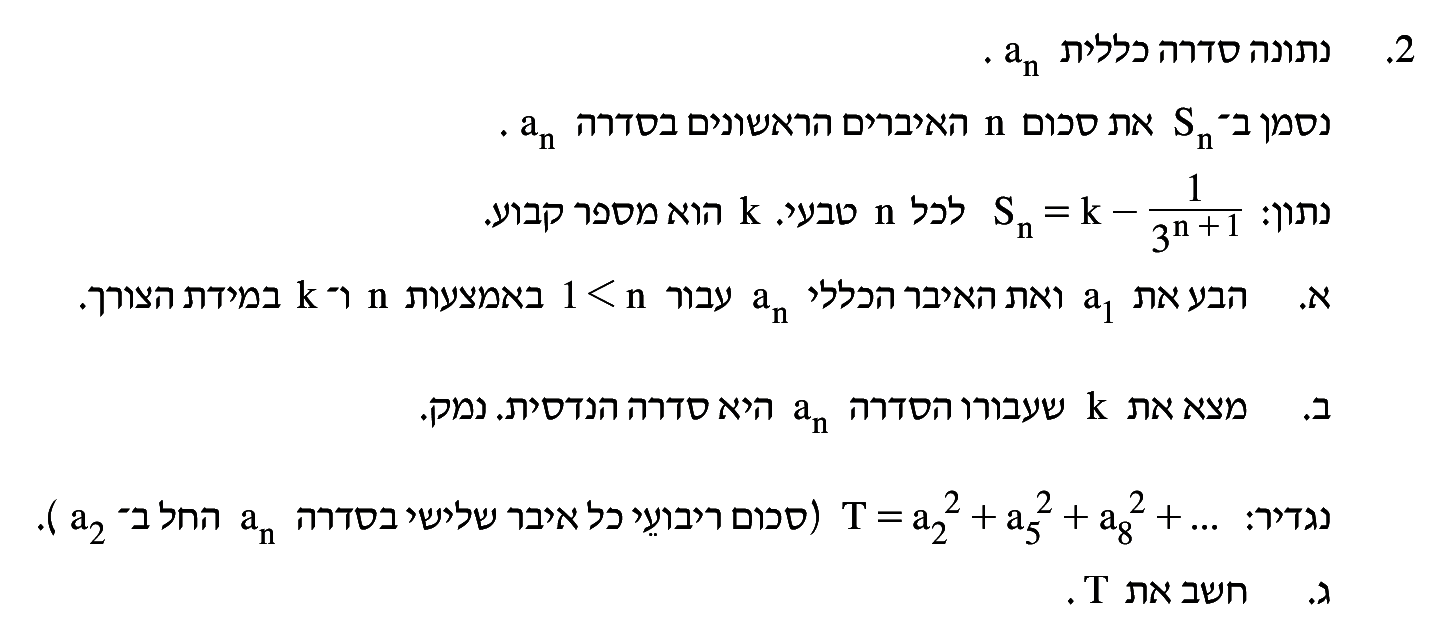
\includegraphics[width=.95\textwidth]{summer-2017b-2}
\end{center}

שאלה זו שונה משאלות אחרות כי נתון ביטוי עבור
\textbf{הסכומים}
ולא עבור האיברים בסדרה.

\smallskip

\textbf{סעיף א}

ניתן לחשב את האיברים על ידי שימוש בנוסחה עבור
$S_n$.
האיבר הראשון מתקבל ישירות מהנוסחה:
\[
a_1=S_1=k-\frac{1}{3^{1+1}}=k-\frac{1}{9}\,,
\]
והאיבר הכללי מתקבל על ידי ההפרש בין הנוסחאות לסכומים עוקבים:
\[
a_n=S_{n}-S_{n-1}=\left(k-\frac{1}{3^{n+1}}\right)-\left(k-\frac{1}{3^{n}}\right)=\frac{2}{3^{n+1}}\,.
\]
\textbf{סעיף ב}

המנה
$q=\displaystyle\frac{a_{n+1}}{a_{n}}=\frac{1}{3}$
לא תלויה ב-%
$k$.
במבט ראשון נראה שהתשובה היא שהסדרה היא הנדסית עבור כל ערך של
$k$,
אולם זו טעות. המנה המתקבלת מ-%
$\displaystyle\frac{a_2}{a_1}$
חייבת להיות שווה למנה המתקבלת מהמקרה הכללי
$\displaystyle\frac{a_{n+1}}{a_{n}}$.
נחשב:
\[
\frac{a_2}{a_1}=\frac{\displaystyle\frac{2}{3^3}}{\displaystyle k-\frac{1}{9}} =  \frac{2}{3(9k-1)}=\frac{1}{3} =\frac{a_{n+1}}{a_n}\,.
\]
הפתרון היחיד הוא
$\displaystyle k=\frac{1}{3}$.

עבור הסעיף הבא נצטרך את האיבר הראשון:
\[
\displaystyle \frac{1}{3}-\frac{1}{9}=\frac{2}{9}\,.
\]

\np

\textbf{סעיף ג}

האיבר הראשון בסדרה החדשה הוא:
\[
a'_1 = a_2^2=\left(a_1q\right)^2=\left(\frac{2}{9}\cdot\frac{1}{3}\right)^2=\frac{4}{729}\,,
\]
הסדרה החדשה היא הנדסית:
\erh{14pt}
\begin{equationarray*}{rcl}
\left(\frac{a_{3(k+1)-1}}{a_{3k-1}}\right)^2 &=& \left(\frac{a_{3k+2}}{a_{3k-1}}\right)^2\\
&=&\left(\frac{qa_{3k+1}}{a_{3k-1}}\right)^2\\
&=&\left(\frac{q^2a_{3k}}{a_{3k-1}}\right)^2\\
&=&\left(\frac{q^3a_{3k-1}}{a_{3k-1}}\right)^2=q^6=\left(\frac{1}{3}\right)^6=\frac{1}{729}\,.
\end{equationarray*}
הסכום מתקבל מהנוסחה לסדרה הנדסית אינסופית עבור
$a', q'$:
\[
S'=\frac{a'_1}{1-q'}=
\frac{\displaystyle\frac{4}{729}}{1-\displaystyle\frac{1}{729}}= \frac{1}{182}\,.
\]

%%%%%%%%%%%%%%%%%%%%%%%%%%%%%%%%%%%%%%%%%%%%%%%%%%%%%%%%%%%%%%%%%%%
\np
\section{קיץ תשע"ז מועד א}

\begin{center}
\selectlanguage{english}
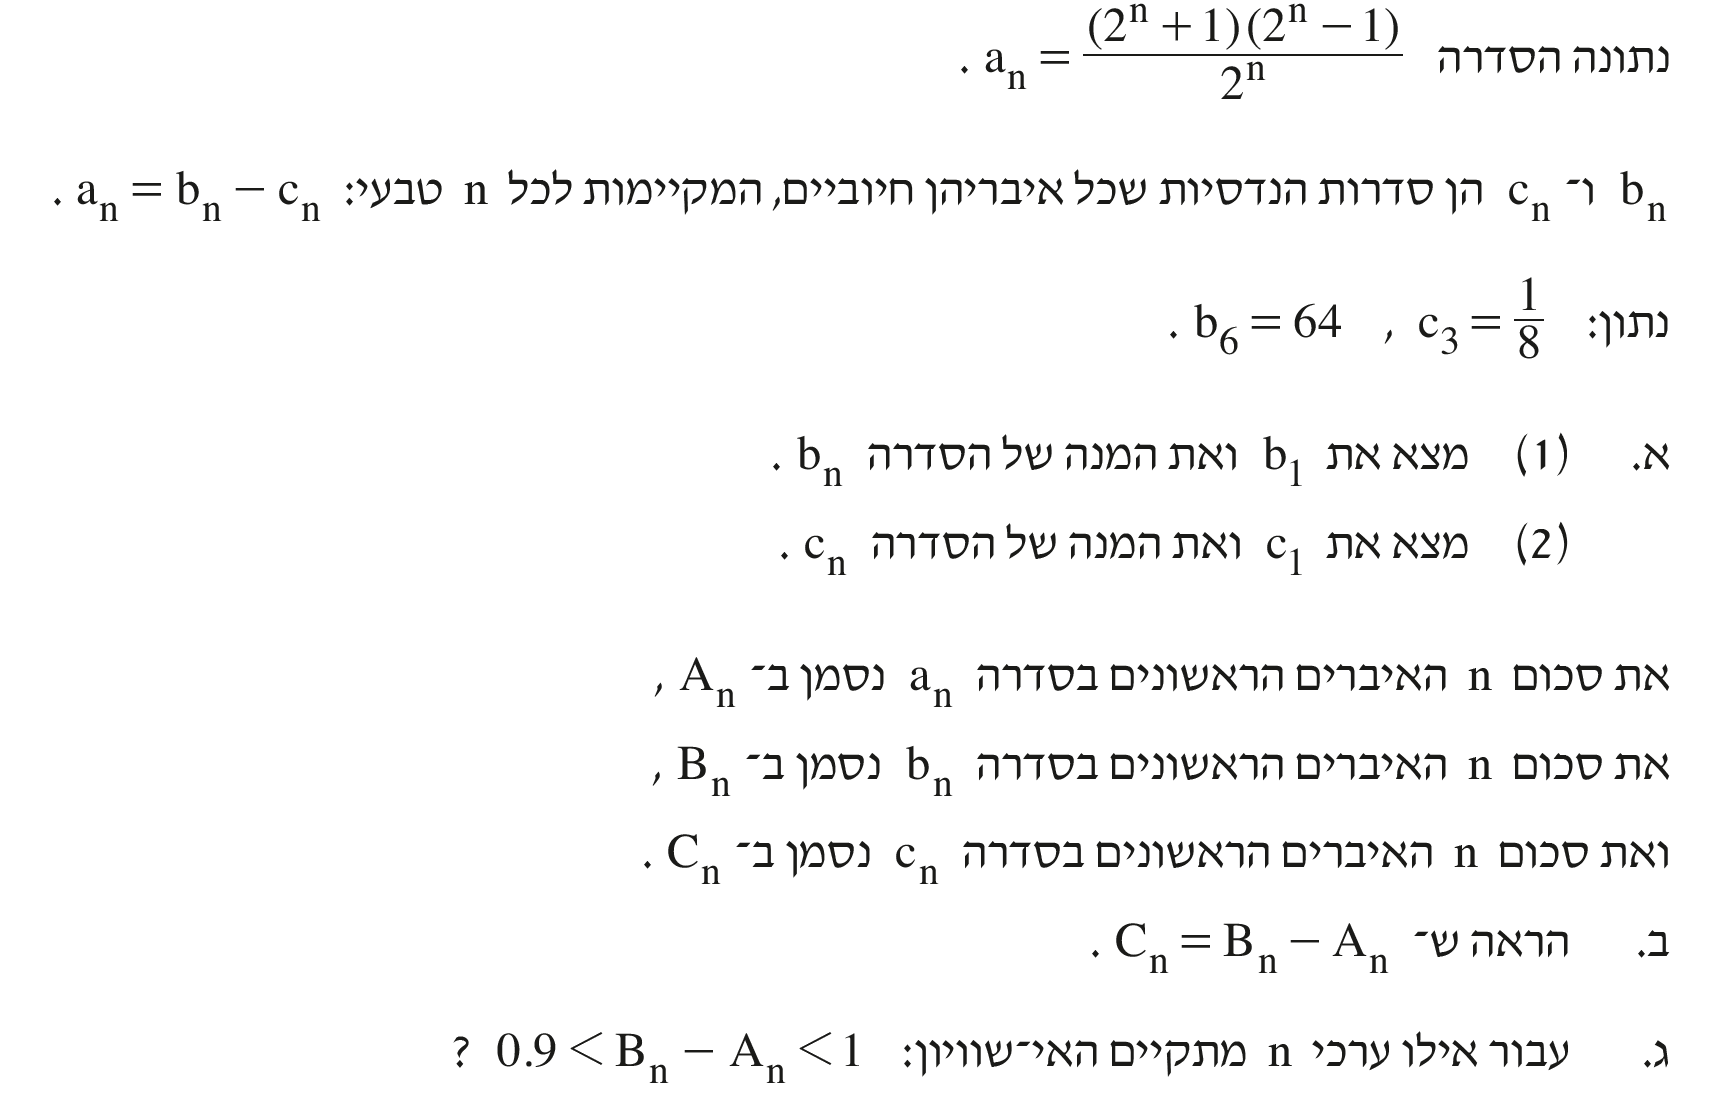
\includegraphics[width=.95\textwidth]{summer-2017a-2}
\end{center}
הנוסחה ל-%
$a_n$
אינה כלל נסיגה כי איברים של הסדרה לא מופיעים בצד הימני של המשוואה. נתון שהסדרות 
$b_n,c_n$
הנדסיות אך לא נתון אם הסדרה המקורית
$a_n$
הנדסית או לא.

\textbf{סעיף א}
$(1,2)$

נתון ש-%
$a_n=b_n-c_n$,
לכן כדי לקבל ערך של איבר בסדרה
$b_n$,
נצטרך לחשב את הערכים
$a_n,c_n$,
ובאופן דומה עבור איברים בסדרה
$c_n$.
נתון שני ערכים
$b_6,c_3$
וקל לחשב איברים ב-%
$a_n$
כי הם נתונים כפונקציה של 
$n$ 
בלבד:
\[
\erh{18pt}
\begin{array}{l@{\hspace{3em}}l}
\displaystyle a_3=\frac{(2^3+1)(2^3-1)}{2^3}=\frac{63}{8}&\displaystyle a_6=\frac{(2^6+1)(2^6-1)}{2^6}= \frac{65\cdot 63}{64}\\
\displaystyle b_3=a_3+c_3=\frac{63}{8}+\frac{1}{8}=8 &\displaystyle  c_6=b_6-a_6=64-\frac{65\cdot 63}{64}=\frac{1}{64}\,.
\end{array}
\]
כדי לחשב את המנה של
$b_n$
והמנה של
$c_n$
נשתמש בנתון שהן סדרות הנדסיות. את האיבר הששי של הסדרות נקבל מהאיבר השלישי על ידי הכפלתו במנה לחזקה שלוש:
\vspace{-1ex}
\[
\erh{22pt}
\begin{array}{l@{\hspace{1em}}l@{\hspace{4em}}l@{\hspace{1em}}l}
b_6=b_3q_b^3, &
\displaystyle q_b=\sqrt[3]{\frac{b_6}{b_3}}=\sqrt[3]{8}=2&
b_3=b_1 q_b^2, &
\displaystyle b_1=\frac{b_3}{q_b^2}=\frac{8}{4}=2\\
c_6=c_3q_c^3, &
\displaystyle q_c=\sqrt[3]{\frac{c_6}{c_3}} =\sqrt[3]{\frac{1}{8}} = \frac{1}{2}&
c_3=c_1 q_c^2 &
\displaystyle c_1=\frac{c_3}{q_c^2}=\frac{1/8}{1/4}=\frac{1}{2}\,.
\end{array}
\]

\np

\textbf{סעיף ב}

הטיעון נובע מחוקי הקיבוץ והחילוף של מספרים שלמים:
\begin{eqnarray*}
C_n &=& (b_1-a_1) + (b_2 - a_2) + \cdots + (b_n-a_n)\\
&=&(b_1 + b_2 + \cdots + b_n) - (a_1 + a_2 + \cdots + a_n)\\
&=& B_n - A_n\,.
\end{eqnarray*}
\textbf{סעיף ג}

הוכחנו ש-%
$C_n=B_n-A_n$,
ונתונה שהסדרה 
$c_n$
הנדסית. מסעיף א
$\displaystyle q_c=\frac{1}{2},\,c_1=\frac{1}{2}$,
ולכן:
\[
C_n = \frac{1}{2}\cdot\frac{\displaystyle\left(\left(\frac{1}{2}\right)^n-1\right)}{\displaystyle\left(\frac{1}{2}-1\right)}=1-2^{-n}\,.
\]
בדיקה במחשבון מראה ש:
%\vspace{-2ex}
\[
\erh{8pt}
\begin{array}{l}
0.9 \not< 1-2^{-3}=0.875<1\\
0.9 < 1-2^{-4}=0.938 < 1\,.
\end{array}
\]

לא לעצור כאן! השאלה מבקשת את
\textbf{כל הערכים}
של
$n$
המקיימים את האי-שוויון, ולכן התשובה המליאה היא כל מספר גדול או שווה ל-%
$4$,
כי כאשר 
$n$
גדל מעל ל-%
$4$,
הערך של 
$1-2^{-n}$
עולה )ולכן גדול מ-%
$0.9$(
אבל תמיד פחות מ-%
$1$.

%%%%%%%%%%%%%%%%%%%%%%%%%%%%%%%%%%%%%%%%%%%%%%%%%%%%%%%%%%%%%%%%%%%
\np
\section{חורף תשע"ז}

\begin{center}
\selectlanguage{english}
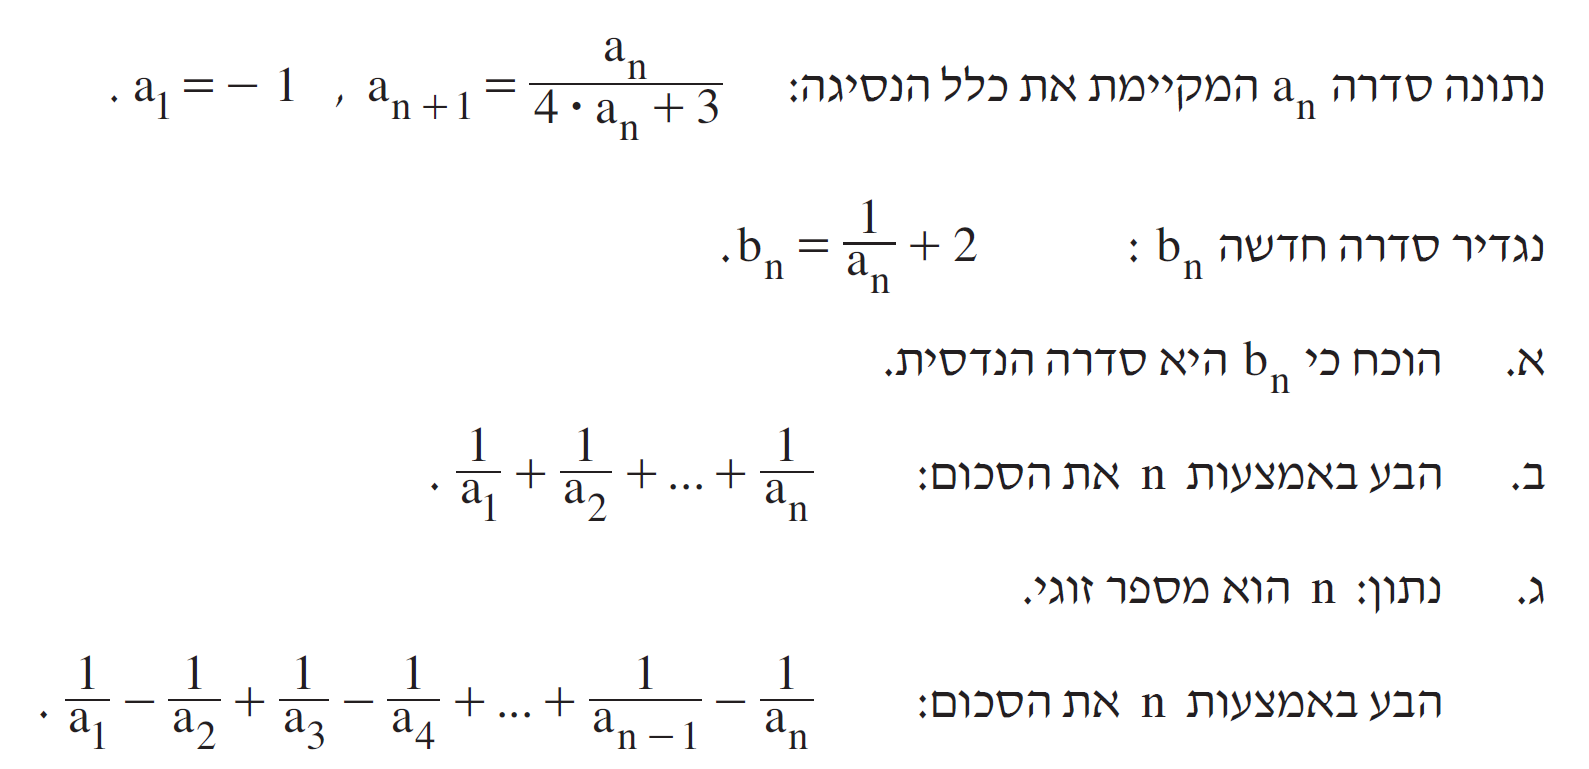
\includegraphics[width=.9\textwidth]{winter-2017-2}
\end{center}

\vspace{-2ex}

\textbf{סעיף א}

נחשב את המנה על ידי הצבה עבור 
$b_n$
לפי ההגדרה, ואחר כך הצבה עבור 
$a_{n+1}$
לפי כלל הנסיגה. נקבל מנה קבועה ולכן הסדרה הנדסית:
\[
\frac{b_{n+1}}{b_n} = \frac{\displaystyle\frac{1}{a_{n+1}}+2}{\displaystyle\frac{1}{a_{n}}+2}= \frac{\displaystyle\frac{4a_n+3}{a_n}+2}{\displaystyle\frac{1}{a_{n}}+2}=\frac{3(2a_n+1)}{2a_n+1}=3\,.
\]
\vspace{-3ex}

\textbf{סעיף ב}

לא נתון שהסדרה $a_n$ הנדסית, אבל בסעיף א הוכחנו שהסדרה  
$b_n$
הנדסית, ולכן ניתן לבטא את סכום הסדרה
$\displaystyle\frac{1}{a_n}$
כסכום של הסדרה
$b_n$
על ידי ההצבה 
$\displaystyle\frac{1}{a_i} = b_i - 2$:
\[
\frac{1}{a_1} + \cdots + \frac{1}{a_n}=(b_1-2) + \cdots + (b_n-2)=b_1+\cdots+b_n- 2n\,.
\]
נתון ש
$a_1=-1$,
כך ש-%
$b_1=\displaystyle\frac{1}{a_1}+2=1$
ובסעיף א חישבנו 
$q_b=3$.
סכום הסדרה של 
$\displaystyle \frac{1}{a_n}$
הוא:
\[
b_1+\cdots+b_n- 2n=\frac{1(3^n-1)}{3-1} - 2n = \frac{3^n - 4n -1}{2}\,.
\]
\textbf{סעיף ג}

לפי ההגדרה של 
$b_n$
נוכל לבטא את הסכום כך:
\[
(b_1 - 2) - (b_2 - 2) + \cdots + (b_{n-1} - 2) - (b_n - 2)\,.
\]
נתון שמספר האיברים זוגי ולכן סכום הקבועים מתאפס. המנה של הסדרה היא
$-3$
והסכום הוא:
\[
b_1-b_2+\cdots+b_{n-1}-b_n=\frac{1((-3)^n-1)}{-3-1}=\frac{(-3)^n-1}{-4}=\frac{1-3^n}{4}\,,
\]
כי מספר האיברים זוגי ולכן
$(-3)^n=3^n$.


%%%%%%%%%%%%%%%%%%%%%%%%%%%%%%%%%%%%%%%%%%%%%%%%%%%%%%%%%%%%%%%%%%%

\np
\section{קיץ תשע"ו מועד ב}

\begin{center}
\selectlanguage{english}
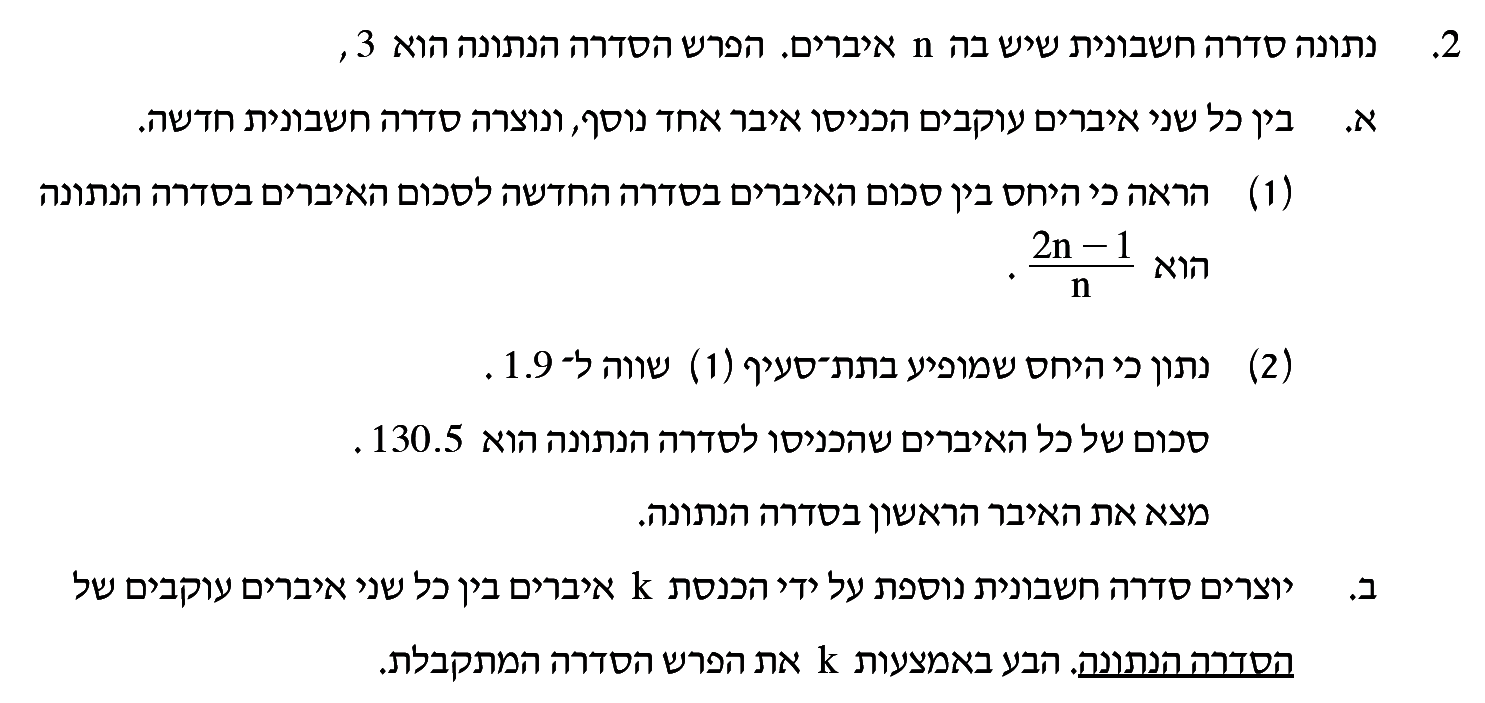
\includegraphics[width=.95\textwidth]{summer-2016b-2}
\end{center}
\vspace{-1ex}

\textbf{סעיף א}
$(1)$

מספר האיברים החדשים הוא
$n-1$,
כפי שרואים אם רושמים את הסדרה:
\[
a_1,\; a'_1,\; a_2,\; a'_2,\; \ldots,\; a_{n-1},\; a'_{n-1},\; a_n\,.
\]
נתון שהסדרה החדשה גם היא חשבונית. הפרש הסדרה אינו מספר שלם אלא
$1.5$!
אז מה? נחשב את היחס בין סכומי הסדרות, כאשר האיבר
$a_1$
מצטמצם:
\[
\frac{S_{\mathit{new}}}{S_{\mathit{old}}}= \frac{\displaystyle\frac{2n-1}{2}(2a_1+1.5((2n-1)-1))}{\displaystyle\frac{n}{2}(2a_1+3(n-1))}=\frac{\displaystyle\frac{2n-1}{2}(2a_1+3(n-1))}{\displaystyle\frac{n}{2}(2a_1+3(n-1))}=\frac{2n-1}{n}\,.
\]
\textbf{סעיף א}
$(2)$

מ-%
$\displaystyle\frac{2n-1}{n}=1.9$
נקבל
$n=10$. 
אם הסדרה הנתונה חשבונית וגם הסדרה החדשה חשבונית, סדרת האיברים החדשים היא חשבונית עם אותו הפרש כמו בסדרה המקורית, 
$3$.
%
%נתון שהסדרה החדשה חשבונית ולכן גם סדרת האיברים החדשים חשבונית:
%\[
%a'_{i+1}-a'_{i}=a'_{i+1}-(a_{i+1}-a_{i+1})-a'_i=(a'_{i+1}-a_{i+1})+(a_{i+1}-a'_i)=\frac{d}{2}+\frac{d}{2}=3\,.
%\]
האיבר הראשון של האיברים החדשים הוא
$a'_1=a_1+1.5$,
ונתון סכום האיברים החדשים:
\[
\frac{10-1}{2}(2(a_1+1.5)+((10-1)-1)\cdot 3) = 130.5\,,
\]
והפתרון הוא
$a_1=1$.

\textbf{סעיף ב}

נתון שהסדרה המתקבלת לאחר הכנסת
$k$
איברים חדשים בין איברים סמוכים של הסדרה הנתונה:
\[
a_i,\; b_1,\; b_2,\; \ldots,\; b_k,\; a_{i+1}
\]
היא חשבונית. ההפרשים בין האיברים החדשים חייבים להיות שווים וסכומם שווה להפרש של הסדרה הנתונה שהוא
$3$.
יש
$k+1$
הפרשים שערכם
$\displaystyle\frac{3}{k+1}$.

%%%%%%%%%%%%%%%%%%%%%%%%%%%%%%%%%%%%%%%%%%%%%%%%%%%%%%%%%%%%%%%%%%%

\np
\section{קיץ תשע"ו מועד א}

\begin{center}
\selectlanguage{english}
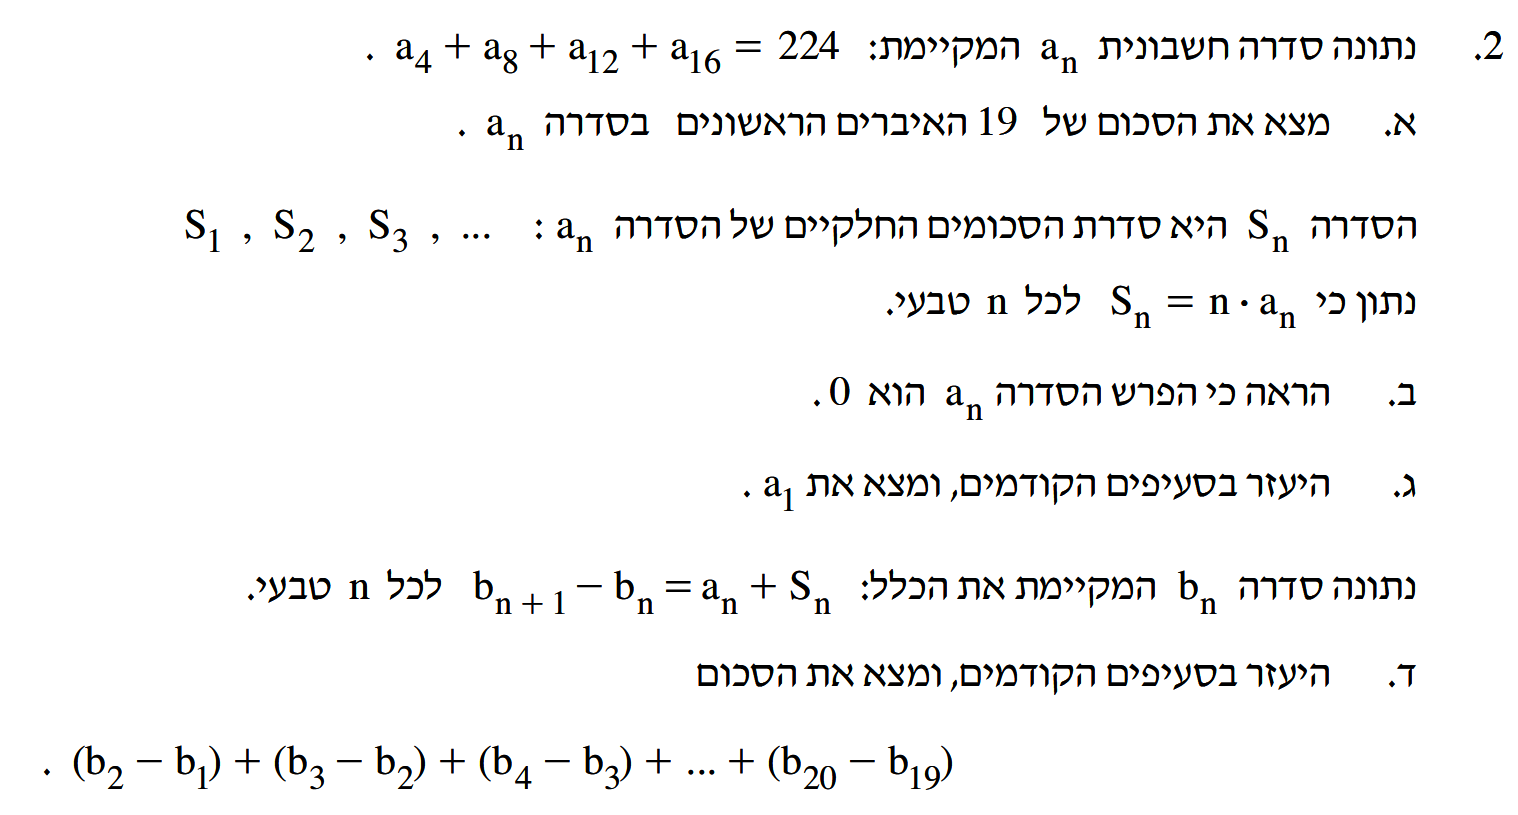
\includegraphics[width=.95\textwidth]{summer-2016a-2}
\end{center}
\vspace{-4ex}

\textbf{סעיף א}

האיברים
$a_4,a_8,a_{12},a_{16}$
מהווים סדרה חשבועית עם הפרש
$d^4$.
נתון הסכום של הסדרה:
\begin{eqnarray*}
(a_1+3d)+(a_1+7d)+(a_1+11d)+(a_1+15d)&=&224\\
a_1+9d&=&56\,.
\end{eqnarray*}
יש לנו משוואה אחת עם שני נעלמים. לא נתייאש וננסה בכל זאת לחשב את הסכום
$S_{19}$:
\[
S_{19}=\frac{19}{2}(2a_1+18d) = 19(a_1+9d)=19\cdot 56 = 1064\,.
\]
\vspace{-1ex}
\textbf{סעיף ב}

נשווה את המשוואה הנתונה
$S_n=n\cdot a_n$
לנוסחה עבור סכום של סדרה חשבונית:
\[
S_n=\frac{n}{2}(2a_1+(n-1)d)=n\cdot a_n= n(a_1+(n-1)d) \,.
\]
%\erh{10pt}
%\begin{equationarray*}{rcl}
%n\cdot a_n &=& \frac{n}{2}(2a_1+(n-1)d)\\
%n(a_1+(n-1)d) &=&\frac{n}{2}(2a_1+(n-1)d)\,.
%\end{equationarray*}
נפשט את המשוואה ונקבל 
$d=d/2$
שהפתרון היחיד שלה הוא
$d=0$.

\textbf{סעיף ג}

נציב
$0$
עבור 
$d$:
$a_1+9d=a_1+0=56$.

\textbf{סעיף ד}

במבט ראשון נראה שכדאי לצמצם את סכום הסדרה  ל-%
$b_{20}-b_1$,
אבל זה מבוי סתום כי אין לנו דרך לחשב את איברי הסדרה
$b_n$.
במקום זה נחשב את 
$(b_{i+1}-b_i)$
וניעזר במשוואה הנתונה:
\[
b_{i+1}-b_i=a_i+S_i=(a_1+(i-1)\cdot 0)+\frac{i}{2}(2a_1+(i-1)\cdot 0)=a_1(1+i)\,.
\]
הסכום הוא:
\[
a_1(2+3+\cdots+20)=56\cdot\frac{19}{2}(2\cdot 2 + (19-1)\cdot 1)=11704\,.
\]

%%%%%%%%%%%%%%%%%%%%%%%%%%%%%%%%%%%%%%%%%%%%%%%%%%%%%%%%%%%%%%%%%%%
\np
\section{חורף תשע"ו}

\begin{center}
\selectlanguage{english}
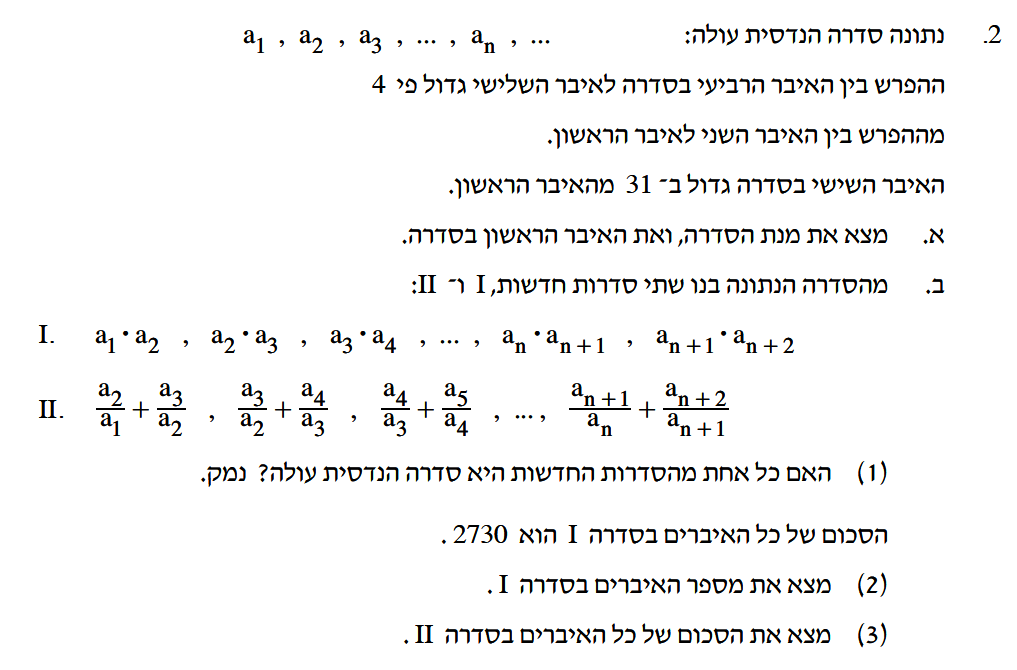
\includegraphics[width=.95\textwidth]{winter-2016-2}
\end{center}

\vspace{-3ex}

\textbf{סעיף א}

נתון:
\[
(1)\, a_4-a_3 = 4 (a_2-a_1),\quad (2)\, a_6 - a_1 = 31\,.
\]
נציב
$a_n=a_1q^{n-1}$ 
עבור
$a_2, a_3, a_4$,
ב-%
$(1)$,
ונקבל שלוש תשובות
$q=1,q=2,q=-2$.\\
נתון שהסדרה 
\textbf{עולה}
ולכן
$q=2$.
נציב 
$a_1q^5=32 a_1$
עבור
$a_6$
ב-%
$(2)$,
ונקבל
$a_1=1$.

\textbf{סעיף ב} 
$(1)$

עבור סדרה I:
\[
q_I=\frac{a_{n+1}\cdot a_{n+2}}{a_n\cdot a_{n+1}}=\frac{a_{n+2}}{a_n}=\frac{a_n\,q^2}{a_n}=q^2=4\,,
\]
והסדרה היא סדרה הנדסית עולה. עבור סדרה II:
\[
q_{II}=\left(\frac{a_{n+1}}{a_n} + \frac{a_{n+2}}{a_{n+1}}\right) / \left(\frac{a_{n}}{a_{n-1}} + \frac{a_{n+1}}{a_{n}}\right)=\frac{q+q}{q+q}=1\,.
\]
הסדרה הנדסית אבל
\textbf{לא עולה}.

\textbf{סעיף ב}
$(2)$

מסכום הסדרה ניתן לחשב את מספר האיברים בסדרה:
\begin{eqnarray*}
a_1\cdot a_2 + \cdots + a_{n+1} \cdot a_{n+2} &=& 2730\\
(1\cdot 2)\cdot \frac{4^{n+1}-1}{4-1}&=&2730\\
4^{n+1}&=&4096\\
n&=&5\,.
\end{eqnarray*}

\np

\textbf{שימו לב!}
אמנם
$n=5$
אבל מספר האיברים בסדרה I הוא 
$n+1=6$:
\[
(1)\, a_1\cdot a_2,\;\; (2)\,a_2\cdot a_3,\;\;(3)\, a_3\cdot a_4,\;\; (4)\,a_4\cdot a_5,\;\; (5)\,a_5\cdot a_6,\;\; (6)\,a_6\cdot a_7 \;(= a_{n+1}\cdot a_{n+2})\,.
\]
\textbf{סעיף ב}
$(2)$

חישבנו
$q_{II}=1$.
נחשב את
$a_1^{II}$:
\[
a_1^{II}=\frac{a_{2}}{a_1} + \frac{a_{3}}{a_{2}}=\frac{2}{1}+\frac{4}{2}=4\,.
\]
\textbf{שימו לב!}
מספר האיברים בסדרה II הוא 
$5$:
\[
(1)\,\frac{a_2}{a_1}+\frac{a_3}{a_2},\;\;
(2)\,\frac{a_3}{a_2}+\frac{a_4}{a_3},\;\;
(3)\,\frac{a_4}{a_3}+\frac{a_5}{a_4},\;\;
(4)\,\frac{a_5}{a_4}+\frac{a_6}{a_5},\;\;
(5)\,\frac{a_6}{a_5}+\frac{a_7}{a_6} \left(= \frac{a_{n+1}}{a_n}+\frac{a_{n+2}}{a_{n+1}}\right)\,.
\]
ולכן סכום האיברים הוא:
\[
(a_1^{II})+(a_1^{II}\cdot 1^1) + (a_1^{II}\cdot 1^2) + (a_1^{II}\cdot 1^3) + (a_1^{II}\cdot 1^4) =  5a_1^{II}=20\,.
\]


%%%%%%%%%%%%%%%%%%%%%%%%%%%%%%%%%%%%%%%%%%%%%%%%%%%%%%%%%%%%%%%%%%%
\np

\section{קיץ תשע"ה, מועד ב}

\begin{center}
\selectlanguage{english}
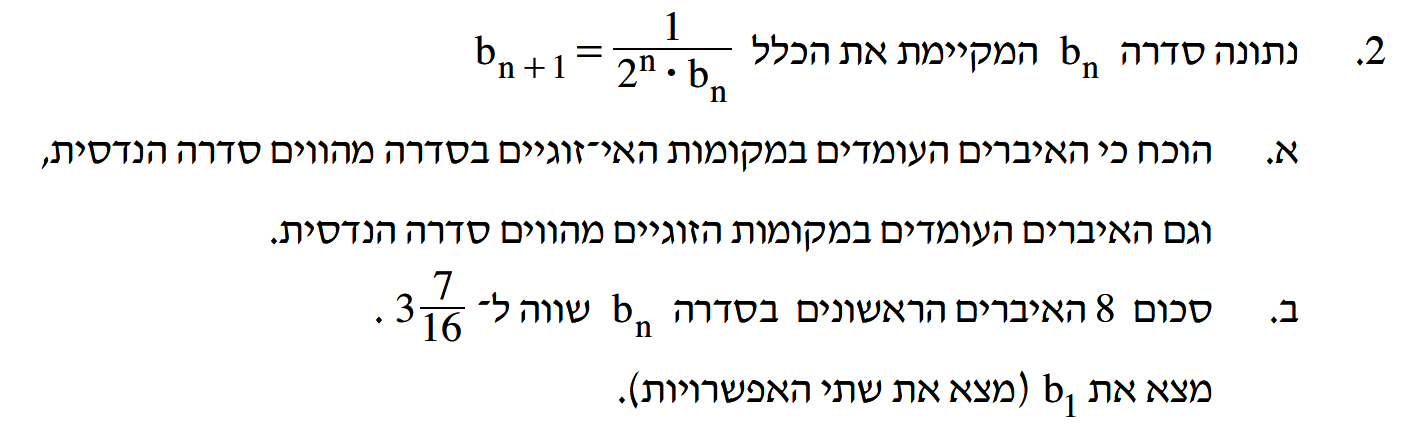
\includegraphics[width=.95\textwidth]{summer-2015b-2}
\end{center}
\vspace{-2ex}

\textbf{סעיף א}

החילוק של איברים במרחק שני מקומות אחד מהשני לא תלוי בזוגיות:
\[
\frac{b_{n+2}}{b_n} = \frac{1}{2^{n+1}b_{n+1}}\cdot\frac{1}{b_n}=\frac{1}{2^{n+1}\cdot\displaystyle\frac{1}{2^nb_n}{b_n}}= \frac{1}{2}\,.
\]
\textbf{סעיף ב}

לא נתון שהסדרה 
$b_n$
הנדסית, ולכן יש לחשב בנפרד את הסכום של ארבעת האיברים הזוגיים וארבעת האיברים האי-זוגיים:
\begin{eqnarray*}
S_{\mathit{odd}} &=& b_1+b_3+b_5+b_7=b_1\left(1 + \frac{1}{2} + \frac{1}{4} +\frac{1}{8}\right)=\frac{15}{8}b_1\\
S_{\mathit{even}} &=& b_2+b_4+b_6+b_8=b_2\left(1 + \frac{1}{2} + \frac{1}{4} +\frac{1}{8}\right)=\frac{15}{8}b_2=\frac{15}{8}\cdot\frac{1}{2^1b_1}\,.
\end{eqnarray*}
מ:
\[
S_{\mathit{odd}} + S_{\mathit{even}} =\frac{15}{8}\left(b_1+\frac{1}{2b_1}\right)= 3\frac{7}{16}=\frac{55}{16}\,,
\]
נקבל משוואה ריבועית 
$6b_1^2-11b_1+3=0$
שיש לה שני פתרונות 
$b_1=\disfrac{3}{2},\,\disfrac{1}{3}$.


%%%%%%%%%%%%%%%%%%%%%%%%%%%%%%%%%%%%%%%%%%%%%%%%%%%%%%%%%%%%%%%%%%%
\np

\section{קיץ תשע"ה מועד א}

\begin{center}
\selectlanguage{english}
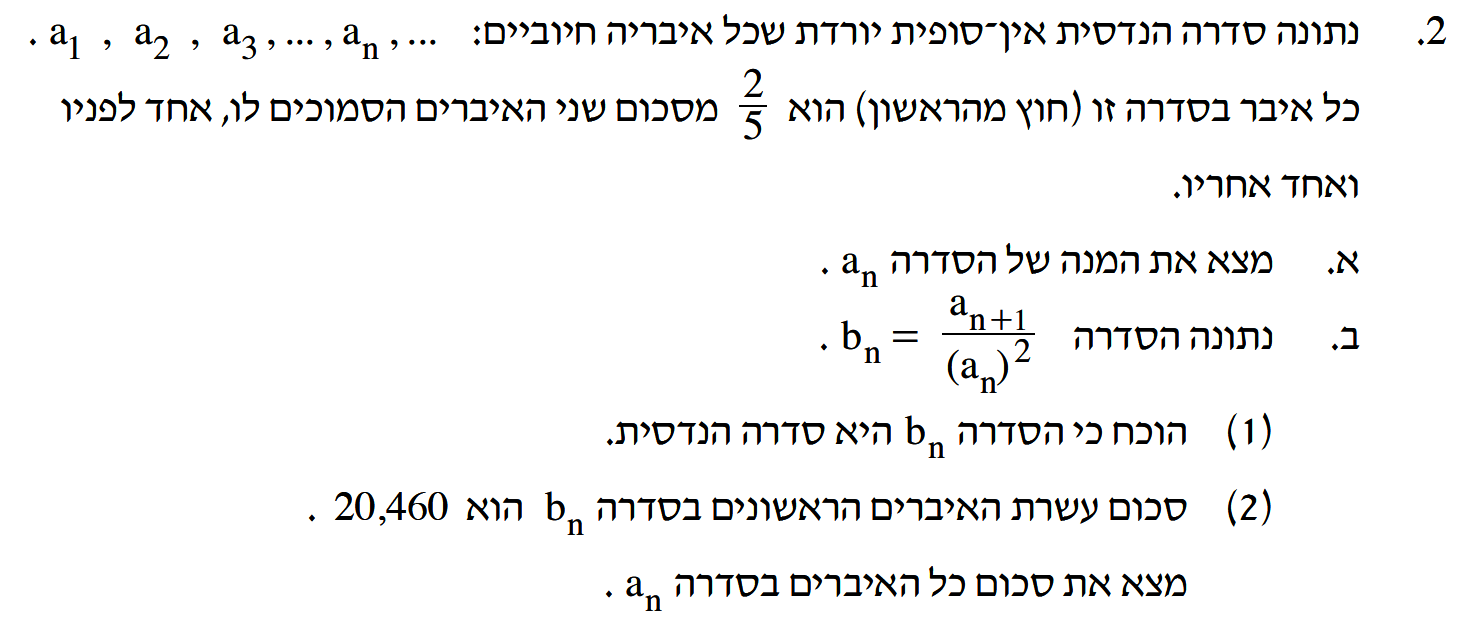
\includegraphics[width=.95\textwidth]{summer-2015a-2}
\end{center}
\vspace{-2ex}

\textbf{סעיף א}

נתון:
\[
a_n = \frac{2}{5}(a_{n-1}+a_{n+1}) =\frac{2}{5}\left(\frac{a_n}{q}+qa_n\right)
\]
עבור
$n\geq 2$.
$a_n$
מצטמצם ונקבל משוואה ריבועית
$2q^2-5q+2=0$
שיש לה שני פתורונות
$\displaystyle q=\frac{1}{2},	q=2$.
נתון שהסדרה יורדת ולכן
$\displaystyle q=\frac{1}{2}$.

\medskip

\textbf{סעיף ב}
$(1)$
\[
\frac{b_{n+1}}{b_n} = \frac{\displaystyle\frac{a_{n+2}}{(a_{n+1})^2}}{\displaystyle\frac{(a_{n})^2}{a_{n+1}}}= \frac{a_{n+2}}{(a_{n+1})^2}\cdot\frac{(a_{n})^2}{a_{n+1}} = \frac{a_nq^2}{(a_nq)^2}\cdot\frac{(a_n)^2}{a_nq}=\frac{1}{q}=2\,.
\]
\textbf{סעיף ב}
$(2)$

מ:
\[
S_{10}=\frac{b_1(2^{10}-1)}{2-1}=20460
\]
מתקבל
$b_1=20$.
השאלה מבקשת את סכום 
\textbf{הסדרה המקורית}
$a_{n}$.
כבר חישבנו את המנה שלה
$q=\frac{1}{2}$,
וניתן לחשב את האיבר הראשון מהנוסחה עבור 
$b_n$:
\erh{16pt}
\begin{equationarray*}{rcl}
b_1 &=& \frac{a_2}{a_1^2} = \frac{a_1q}{(a_1)^2} = \frac{1}{2a_1}\\
a_1&=&\frac{1}{2b_1}=\frac{1}{40}\\
S_a &=& \frac{a_1}{1-q}=\frac{1}{40\left(1-\displaystyle\frac{1}{2}\right)} = \frac{1}{20}\,.
\end{equationarray*}

%%%%%%%%%%%%%%%%%%%%%%%%%%%%%%%%%%%%%%%%%%%%%%%%%%%%%%%%%%%%%%%%%%%%
%
\np
\section{חורף תשע"ה}

\begin{center}
\selectlanguage{english}
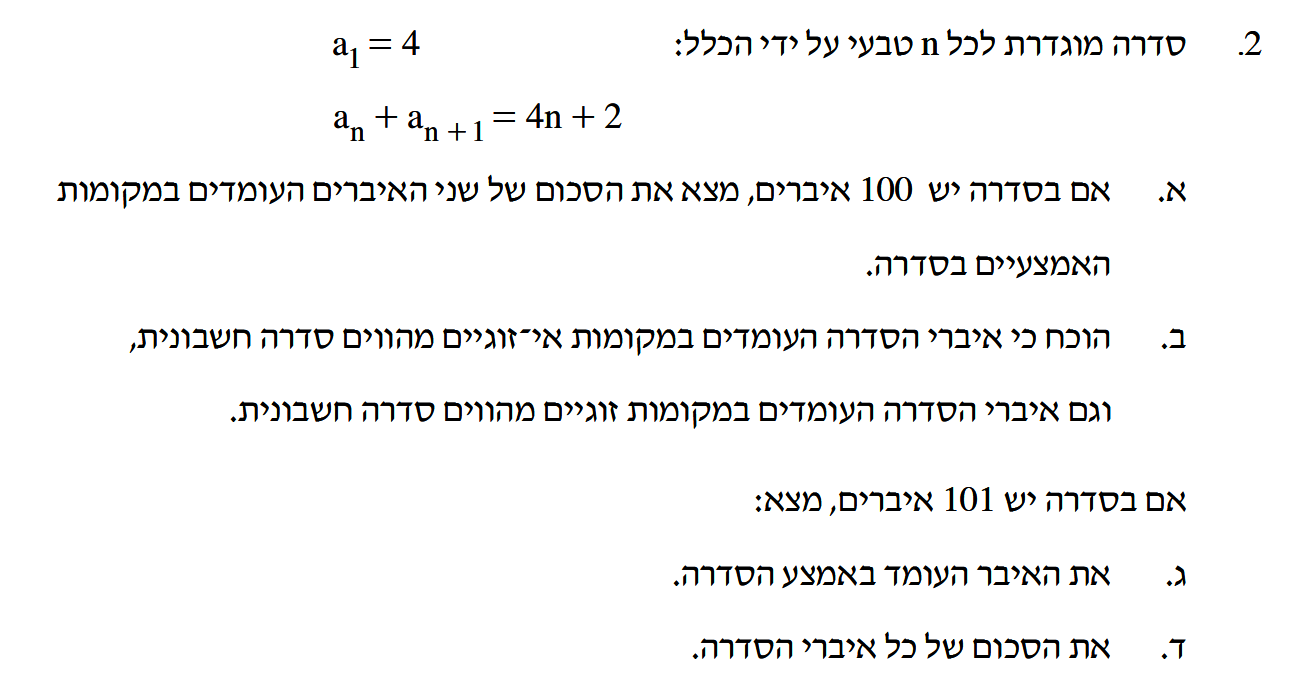
\includegraphics[width=.95\textwidth]{winter-2015-2}
\end{center}
\vspace{-1ex}

\textbf{שימו לב}
שלא נתון שהסדרה
$a_n$
חשבונית.

\textbf{סעיף א}

כדאי לרשום את איברי הסדרה כדי לוודא מהם האיברים האמצעיים:
\[
\overbrace{\rule{0pt}{8pt}a_1, a_2, \ldots, a_{49}, a_{50}}^{50}, \overbrace{\rule{0pt}{8pt}a_{51}, a_{52},\ldots, a_{100}}^{50}\,.
\]
ניתן לחשב את הסכום מהגדרת הסדרה:
\[
a_{50}+a_{51}=4\cdot 50+2=202\,.
\]
\textbf{סעיף ב}

במבט ראשון השאלה נראית בעייתית כי נתונה נוסחה לחישוב איברים סמוכים זה לזה
$a_n+a_{n+1}$,
אבל האיברים הזוגיים נמצאים במרחק שני מקומות זה מזה וכך גם האיברים האי-זוגיים
$a_{n+2}-a_{n}$.
חבל שאין לנו
$a_{n+1}-a_{n}$
ו-%
$a_{n+2}-a_{n+1}$.
צמד הביטויים האלה יכול לרמוז ל-"טריק" ידוע במתמטיקה: אם נוסיף ונחסיר את אותו ערך לביטוי, ערך הביטוי לא משתנה:
\begin{eqnarray*}
a_{k+2} - a_{k} &=& a_{k+2}+(a_{k+1}-a_{k+1})-a_{k}\\
&=& (a_{k+2}+a_{k+1})-(a_{k+1}+a_{k})\\
&=& (4(k+1)+2)-(4k+2)\\
&=&4\,.
\end{eqnarray*}
ההפרש קבוע ולא תלוי בזוגיות, ולכן הזוגיים והאי-זוגיים מהווים סדרות חשבוניות.

\np

\textbf{סעיף ג}

לא ידוע שהסדרה
$a_{n}$
חשבונית, אבל
$a_{51}$
הוא איבר בסדרת
\textbf{האי-זוגיים}.
נרשום את הסדרה כדי לדייק בספירת האיברים הזוגיים והאי-זוגיים:
\[
\overbrace{\rule{0pt}{8pt}a_1, a_2, \ldots, a_{49}, a_{50}}^{50}, a_{51}, \overbrace{\rule{0pt}{8pt}a_{52}, \ldots, a_{100}, a_{101}}^{50}\,.
\]
ברור שמספר האיברים האי-זוגיים גדול באחד ממספר האיברים הזוגיים,
$51$
אי-זוגיים ו-%
$50$
זוגיים. 
$a_{51}$
הוא האיבר ה-%
$25$
העומד באמצע סדרת האי-זוגיים. האיבר הראשון של סדרת האי-זוגיים נתון,
$a_1=4$,
ואת ההפרש
$d=4$
חישבנו בסעיף הקודם. מכאן:
\[
a_{51}=a_1+25d =4+25\cdot 4=104\,.
\]
\textbf{סעיף ד}

נחשב את סכום הסדרה כחיבור של סכום האי-זוגיים וסכום הזוגיים.
$a_1=4$
נתון, ואת
$a_2$
ניתן לחשב לפי הנוסחה הנתונה
$a_n+a_{n+1}=4n+2$
שהיא
$a_{n+1}=(4n+2)-a_n$:
\[
a_2=a_{1+1}=(4\cdot 1+2)-a_1=2\,.
\]
כבר חישבנו שהפרשים של שתי תת-הסדרות הם 
$4$.
מספר האי-זוגיים הוא
$51$
ומספר הזוגיים הוא
$50$.
הסכום הוא:
\[
S=S_{\mathit{odd}} + S_{\mathit{even}}=\frac{51}{2}(2\cdot 4+50\cdot 4)+\frac{50}{2}(2\cdot 2+49\cdot 4)=5304+5000=10304\,.
\]

%%%%%%%%%%%%%%%%%%%%%%%%%%%%%%%%%%%%%%%%%%%%%%%%%%%%%%%%%%%%%%%%%%%
\np

\section{קיץ תשע"ד מועד ב}

\begin{center}
\selectlanguage{english}
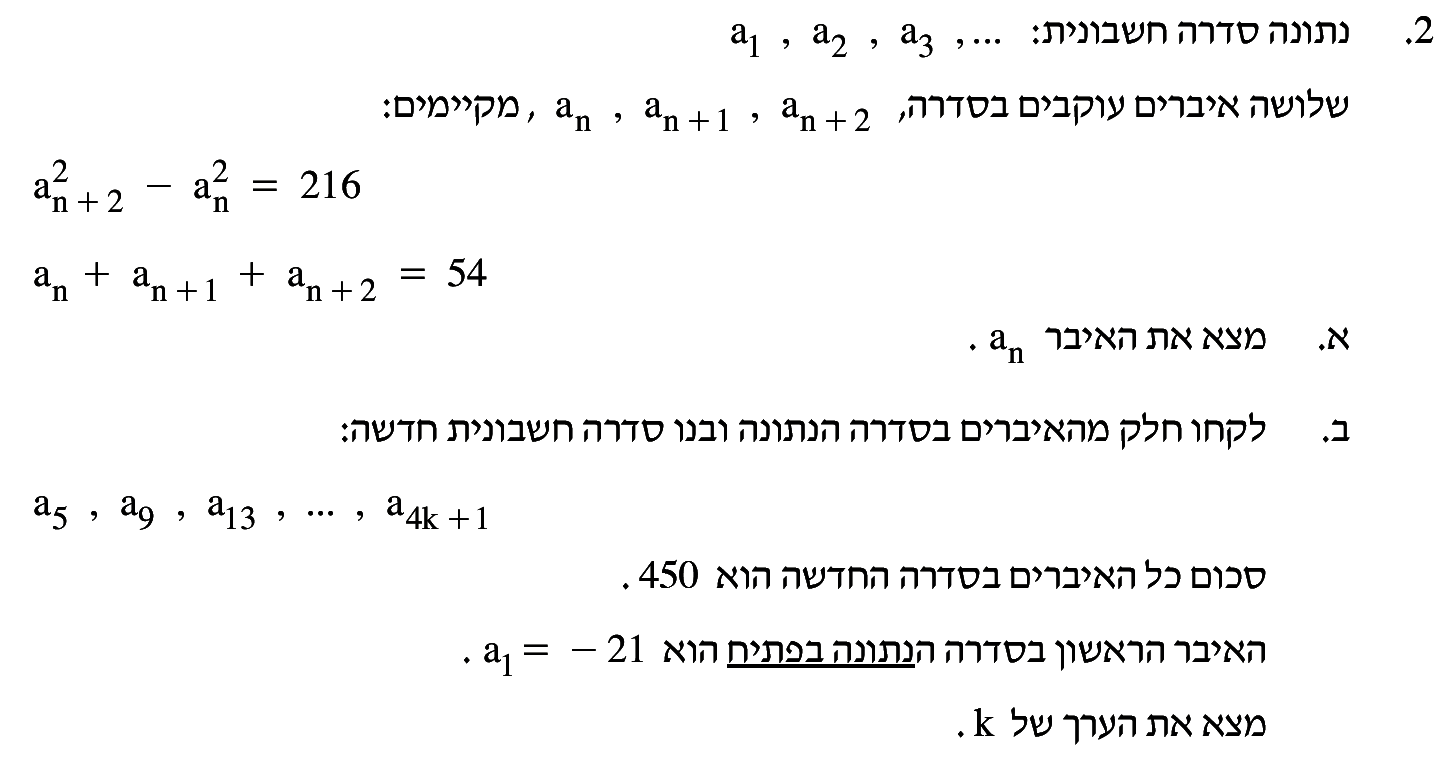
\includegraphics[width=.95\textwidth]{summer-2014b-2}
\end{center}
\vspace{-2ex}


\textbf{סעיף א}

הסדרה חשבונית ולכן ניתן להציב בתוך המשוואות הנתונות ולקבל שתי משוואות עם שני נעלמים:
\erh{4pt}
\begin{equationarray*}{rcl}
(a_n+2d)^2 - a_n^2 &=& 216\\
4a_nd+4d^2 &=& 216\\
a_n+(a_n+d)+(a_n+2d)&=&54\\
3a_n + 3d &=& 54\,.
\end{equationarray*}
הפתרון הוא
$d=3,a_n=15$.

\smallskip

\textbf{סעיף ב}

הסדרה החדשה חשבונית שאיבריה 
$a'_1, a'_2,\ldots$
הם:
\[
\overbrace{a_5=a_1+4d}^{a_1'}, \quad a_6=a_5+5d,\quad  a_7=a_5+6d,\quad  a_8=a_5+7d,\quad  \overbrace{a_9=a_5+8d}^{a_2'}\,.
\]
בסדרה החדשה
$d' = 4d = 12$
ו-%
$a_1' = a_5 = -21 + 4d= -9$.
מסכום הסדרה החדשה:
\[
\frac{k}{2}(2a'_1 + (k-1)d')=\frac{k}{2}(-18+(k-1)\cdot 12)=450,
\]
מתקבלת משוואה ריבועית
$2k^2-5k-150=0$
שהשורש החיובי שלה הוא
$k=10$.


%%%%%%%%%%%%%%%%%%%%%%%%%%%%%%%%%%%%%%%%%%%%%%%%%%%%%%%%%%%%%%%%%%%

\np
\section{קיץ תשע"ד מועד א}

\begin{center}
\selectlanguage{english}
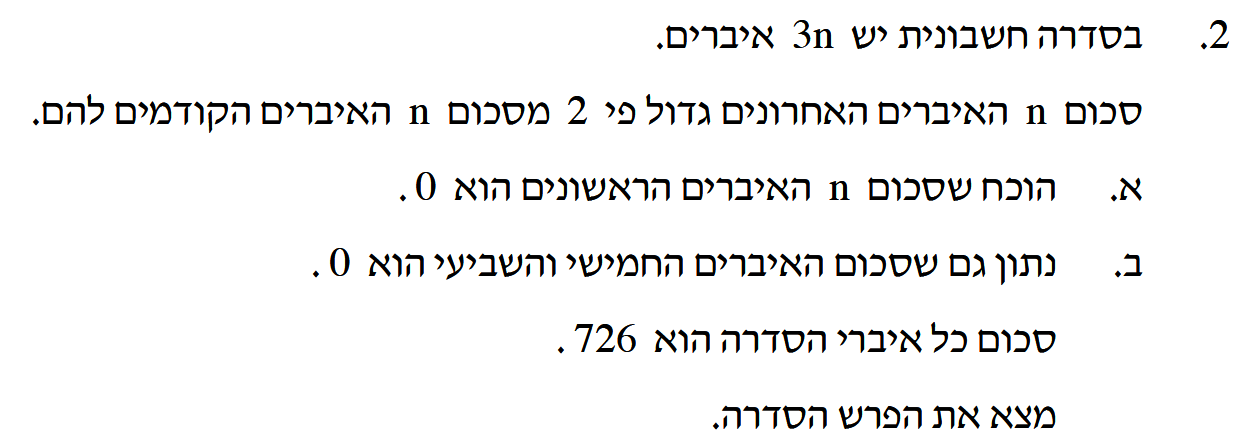
\includegraphics[width=.9\textwidth]{summer-2014a-2}
\end{center}

\vspace{-4ex}

\textbf{סעיף א}

כדי לדייק עם המקומות של האיברים כדאי לרשום את הסדרה עם סימון של הסדרות החלקיות:
\[
\underbrace{
\overbrace{\rule{0pt}{8pt}a_1, a_2, \ldots, a_n}^{S_1},
\overbrace{\rule{0pt}{8pt}a_{n+1}, a_{n+2}, \ldots, a_{2n}}^{S_2},
\overbrace{\rule{0pt}{8pt}a_{2n+1}, a_{2n+2}, \ldots, a_{3n}}^{S_3}
}_{S_{3n}}\,.
\]
נתון
$S_3=2S_2$:
\[
\erh{10pt}
\begin{array}{lll}
\displaystyle\frac{n}{2}(2(a_1+2nd)+(n-1)d)&=&2\cdot \displaystyle\frac{n}{2}(2(a_1+nd)+(n-1)d)\\
2a_1+(5n-1)d&=&4a_1+(6n-2)d\\
2a_1+(n-1)d&=&0\,.
\end{array}
\]
הביטוי בצד השמאלי של המשוואה האחרונה הוא הסכום 
$S_1$.

דרך אחרת לפתור את הבעיה היא להחסיר את סכום התת-הסדרות מסכום הסדרה כולה:
\erh{14pt}
\begin{equationarray*}{rcl}
S_1&=& S_{3n} - (S_2+S_3) =  S_{3n} - (S_2 + 2S_2) = S_{3n} - 3S_2\\
&=&\displaystyle\frac{3n}{2}(2a_1+(3n-1)d) -3\cdot\displaystyle \frac{n}{2}(2(a_1+nd)+(n-1)d)\\
&=&0\,.
\end{equationarray*}

\np

\begin{center}
\fbox{
\begin{minipage}{.8\textwidth}
בבחינה של חורף תשע"ב אורך הסדרה הוא
$2n-1$,
ונתונים הסכומים של
$n$
האיברים הראשונים ו-%
$n$
האיברים האחרונים. רק רישום זהיר של הסדרה יבהיר שיש חפיפה בין שתי תת-הסדרות:
\[
\renewcommand{\arraystretch}{.3}
\begin{array}{ll}
\overbrace{\rule{0pt}{8pt}a_1, a_2, \ldots, a_n}^{n},&\hspace{-9pt}a_{n+1}, a_{n+2}, \ldots, a_{2n-1}\,.\\
&\hspace{-2em}\underbrace{\rule{10em}{0pt}}_{n}
\end{array}
\]
בדוגמה קל יותר לשים לב לחפיפה. עם
$n=4$:
\[
\renewcommand{\arraystretch}{.3}
\begin{array}{ll}
\overbrace{\rule{0pt}{8pt}a_1, a_2, a_3, a_4}^{4},&\hspace{-9pt}a_5, a_6, a_7\,.\\
&\hspace{-2em}\underbrace{\rule{5em}{0pt}}_{4}
\end{array}
\]
\vspace*{-1ex}
\end{minipage}
}
\end{center}

\bigskip

\textbf{סעיף ב}

נתון שסכום הסדרה ועלינו למצוא
$d$
למרות שאין לנו 
$a_1$.
נבדוק אם הנתון השני יכול לעזור:
\[
a_5+a_7=(a_1 + 4d) + (a_1 + 6d) = 0\,.
\]
מכאן ש-%
$a_1=-5d$.


בסעיף א חישבנו ש-%
$S_1=0$
ונציב עבור 
$a_1$:
\[
\frac{n}{2}(-10d+(n-1)d)=0\,.
\]
אם 
$d=0$,
מהנתון
$a_5+a_7=0$
אפשר להסיק שכל איברי הסדרה הם אפס. זה סותר את הנתון שהסכום חיובי. לכן אפשר לחלק את המשוואה ב-%
$d$
ונקבל
$n=11$.

נציב עבור
$a_1,n$
בנוסחה ל-%
$S_{3n}$:
\erh{16pt}
\begin{equationarray*}{rcl}
S_3&=&\frac{3n}{2}(2a_1+(3n-1)d)\\
&=&\frac{33}{2}(-10d+(33-1)d)\\
&=&\frac{33}{2}\cdot 22d = 363d=726\,,
\end{equationarray*}
ונקבל 
$d=2$.

%%%%%%%%%%%%%%%%%%%%%%%%%%%%%%%%%%%%%%%%%%%%%%%%%%%%%%%%%%%%%%%%%%%
\np

\section{חורף תשע"ד}

\begin{center}
\selectlanguage{english}
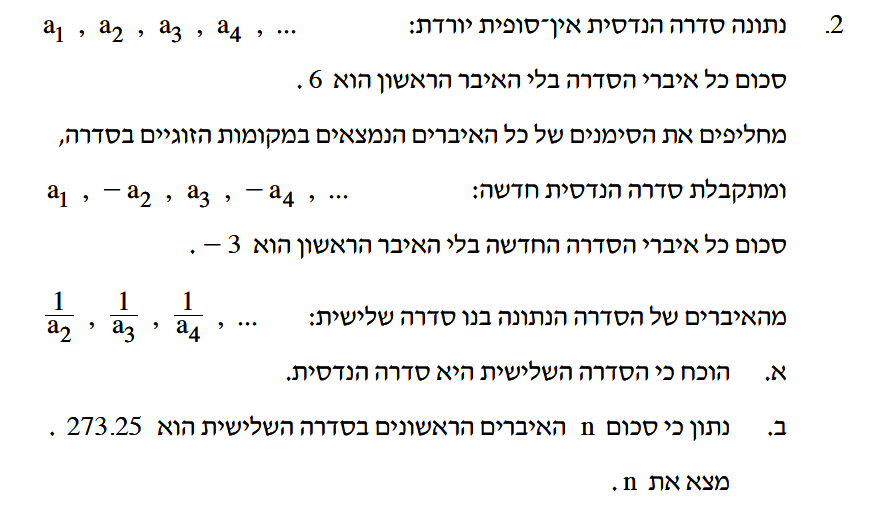
\includegraphics[width=.9\textwidth]{winter-2014-2}
\end{center}
\vspace{-2ex}
\textbf{סעיף א}

המנה של הסדרה השלישית קבועה כי נתון שהסדרה הראשונה הנדסית:
\[
\frac{1/a_{n+1}}{1/a_n}=\frac{a_n}{a_{n+1}}\,.
\]
\textbf{סעיף ב}

נשתמש בשני הסכומים הנתונים כדי לכתוב שתי משוואות עם שני נעלמים:
\erh{12pt}
\begin{equationarray*}{rcl}
\frac{a_2}{1-q}&=&6\\
\frac{-a_2}{1-(-q)}&=& -3\,.
\end{equationarray*}
הפתרון הוא 
$q=\displaystyle\frac{1}{3}$
ו-%
$a_2=4$.

בסדרה השלישית, האיבר הראשון הוא 
$\displaystyle \frac{1}{a_2}=\frac{1}{4}$
וההפרש הוא
$\displaystyle \frac{1}{d}=3$.
מהסכום השלישי ונקבל:
\erh{12pt}
\begin{equationarray*}{rcl}
\frac{1}{4}\cdot \frac{3^n-1}{3-1}&=&273.25\\
3^n&=&2187\\
n&=&7\,,
\end{equationarray*}
כאשר בדקנו חזקות של
$3$
עד שהתקבל
$2187$.



%%%%%%%%%%%%%%%%%%%%%%%%%%%%%%%%%%%%%%%%%%%%%%%%%%%%%%%%%%%%%%%%%%%

\selectlanguage{english}
\clearpage
\selectlanguage{hebrew}

\section*{המלצות}

\addcontentsline{cot}{chapter}{המלצות: סדרות}


\begin{itemize}


\item
\textbf{חובה לקרוא את השאלות בזהירות רבה.}
בבחינה של קיץ תשע"ה א, סעיף ב שואלת על סדרה חדשה
${b_n}$,
אבל בסוף חוזרת ומבקשת למצוא את הסכום של הסדרה הנתונה
${a_n}$.

\item 
ברוב השאלות נתונה סדרה ומוגדרת סדרה חדשה המובססת על הסדרה הנתונה. 
\textbf{אין בהכרח קשר}
בין תכונה של הסדרה המקורית והסדרה החדשה. להלן שתי סדרות חשבוניות, אבל כאשר משלבים את שתיהן, מתקבלת סדרה שאיננה חשבונית:
\[
\begin{array}{rrrrrrrrrrr}
1,& 4,& 7,& 10,& 13,& \ldots\\
2,& 5,& 8,& 11,& 14, &\ldots\\
1,& 2,& 4,& 5,& 7,& 8,& 10,& 11,& 13,& 14, &\ldots
\end{array}
\]
\item
כאשר מבקשים להוכיח שתת-סדרת הזוגיים חשבונית או הנדסית וגם תת-סדרת האי-זוגיים, הוכחה אחת תספיק כי אם 
$\displaystyle \frac{a_{n+2}}{a_n}$
קבוע, לא משנה אם 
$n$
זוגי או אי-זוגי.


\item
כדאי לרשום את איברי הסדרה כדי לדייק במקומות של האיברים:
\[
\setlength{\extrarowheight}{8pt}
\begin{array}{l}
\overbrace{\rule{0pt}{8pt}a_1, a_2, \ldots, a_{49}, a_{50}}^{50}, \overbrace{\rule{0pt}{8pt}a_{51}, a_{52},\ldots, a_{100}}^{50}\\
\underbrace{\rule{0pt}{8pt}a_1, a_2, \ldots, a_{49}, a_{50}}_{50}, a_{51}, \underbrace{\rule{0pt}{8pt}a_{52}, \ldots, a_{100}, a_{101}}_{50}\,.
\end{array}
\]
\vspace{-3ex}

\item
מקרה מעניין הוא תת-סדרות חופפות )בחינה של חורף תשע"ב שלא נמצאת במסמך זה(:
\[
\renewcommand{\arraystretch}{.4}
\begin{array}{ll}
\overbrace{\rule{0pt}{8pt}a_1, a_2, \ldots, a_n}^{n},&\hspace{-9pt}a_{n+1}, a_{n+2}, \ldots, a_{2n-1}\\
&\hspace{-2em}\underbrace{\rule{10em}{0pt}}_{n}
\end{array}
\]
\vspace{-4ex}
\item
קיימות שתי דרכים לסכם מספר תת-סדרות. דרך אחת היא לסכם כל תת-סדרה בנפרד עם ערכי ה-%
$d, a_1$
או
$n, q$
שלהן. זה קורה לעתים קרובות כאשר השאלה מבקשת לחשב סכום של סדרה, אבל ידוע רק שתת-הסדרות חשבוניות או הנדסיות, למשל, זוגיים ואי-זוגיים.

\item 
דרך אחרת היא לחבר את הסכומים של תת-סדרות ולהחסיר את התוצאה מסכום הסדרה כולה:
\[
S_1 = S_n - (S_2+S_3)\,.
\]
\vspace{-6ex}

\item
הבחינה של חורף תשע"ו מעניינת כי מספר האיברים הוא לא הערך של המספר 
$n$
המופיע בשאלה. חשוב לרשום דוגמה מספרית כדי לוודא מהו מספר האיברים:
\[
(1)\, a_1\cdot a_2,\;\; (2)\,a_2\cdot a_3,\;\;\cdots\;\; (5)\,a_5\cdot a_6=(a_n\cdot a_{n+1}),\;\; (6)\,a_6\cdot a_7 \;(= a_{n+1}\cdot a_{n+2})\,.
\]

\np

\item
טריק שימושי הוא לחבר ולהחסיר את אותו ערך בביטוי:
\[
a_{k+2} - a_{k} = a_{k+2}+(a_{k+1}-a_{k+1})-a_{k} = (a_{k+2}+a_{k+1})-(a_{k+1}+a_{k})\,.
\]
\vspace{-4ex}

\item
הכנסת איברים חדשים בתוך סדרה לא בהכרח שומרת על הסדרה כחשבונית או הנדסית. השורה הראשונה להלן היא סדרה חשבונית. בשורה השנייה הוכנסו איברים של סדרה חשבונית נוספת והסדרה החדשה היא חשבונית. בשורה השלישית הוכנסו איברים של סדרה חשבונית נוספת והסדרה החדשה איננה חשבונית.
\[
\begin{array}{rrrrrrrrrrrrr}
1,& 5,& 9,& 13,& 17\\
1, &3,& 5,&7,& 9,& 11,& 13, &15, & 17\\
1, &2,& 5,&6,& 9,& 10,& 13, &14, & 17
\end{array}
\]
\item
בחישוב הפרש או מנה, כדאי להציב עבור
$a_{n+1}$
או
$a_{n-1}$
ביטוי שיש בו 
$a_n$
כדי לקבל משוואה עם נעלם אחד:
\[
a_n = \frac{2}{5}(a_{n-1}+a_{n+1}) =\frac{2}{5}\left(\frac{a_n}{q}+qa_n\right)\,.
\]
$a_n$
מצטמצם ונקבל משוואה ריבועית ב-%
$q$.

\end{itemize}

\npchap


\tikzsetfigurename{probability}
% !TeX root = probability.tex

%%%%%%%%%%%%%%%%%%%%%%%%%%%%%%%%%%%%%%%%%%%%%%%%%%%%%%%%%%%%%%%%

\documentclass[12pt,a4paper,leqno]{article}

\usepackage{verbatim}
\usepackage{url}
\usepackage{fancyhdr}
\usepackage{graphicx}
\usepackage{bm}

\graphicspath{{../images/}}

% TikZ package
\usepackage{tikz}
\usetikzlibrary{arrows.meta,shapes}
\tikzset {>=Stealth}

% Polyglossia Hebrew (main) and English (other)
\usepackage{polyglossia}  
\setmainlanguage{hebrew}
\setotherlanguage{english}

% Fonts: David for Hebrew, Palatino/Courier for English
\newfontfamily{\hebrewfont}{David}[Script=Hebrew]
\newfontfamily{\englishfont}{Palatino Linotype}
\newfontfamily{\englishfonttt}{Courier New}
\newfontfamily{\hebrewfonttt}{Courier New}

% Abbreviations for backwards compatibility with babel
\renewcommand*{\L}[1]{\textenglish{\small #1}}
\newcommand*{\R}[1]{\texthebrew{#1}}

% Use fancyhdr to make all page numbers uniform
\pagestyle{fancy}
\fancyhead{}
\renewcommand{\headrulewidth}{0pt}
\renewcommand{\footrulewidth}{0pt}
\fancyfoot[C]{$\thepage$}

% Displaystyle for fractions and combinations
\newcommand*{\disfrac}[2]{\displaystyle\frac{#1}{#2}}
\newcommand*{\dischoose}[2]{\displaystyle{#1 \choose #2}}

\newcommand*{\bover}[1]{\bm{\overline{#1}}}
\newcommand*{\erh}[1]{\renewcommand{\arraystretch}{#1}}

% Reduce space around c column in eqnarray*
\newenvironment{eqn}
  {\addtolength{\arraycolsep}{-3pt}\begin{eqnarray*}}
  {\end{eqnarray*}}
  
% Reduce space around c column in eqnarray with labels
\newenvironment{eqnlabels}
  {\addtolength{\arraycolsep}{-3pt}
   \begin{eqnarray}}
  {\end{eqnarray}}

% Use english equation numbers in hebrew document
\renewcommand{\theequation}{\L{\arabic{equation}}}

% Allow pages with larger floats
\renewcommand{\floatpagefraction}{.8}

% Layout
\textwidth=155mm
\textheight=230mm
\topmargin=0pt
\headheight=0pt
\oddsidemargin=0mm
\evensidemargin=0mm
\headsep=0pt
\parindent=0pt
\renewcommand{\baselinestretch}{1.1}
\setlength{\parskip}{0.3\baselineskip plus 1pt minus 1pt}

%\includeonly{}

\begin{document}
% !TeX root = probability.tex

\selectlanguage{hebrew}

\thispagestyle{empty}

\begin{center}
\textbf{\LARGE בחינות בגרות בהסתברות}
\end{center}

\bigskip
\bigskip

\begin{center}
\textbf{\Large מוטי בן-ארי}

\bigskip

\url{http://www.weizmann.ac.il/sci-tea/benari/}
\end{center}

\begin{center}	
\begin{bfseries}
\bigskip
\bigskip

\R{גרסה} \L{1.0} 

\bigskip

\today

\end{bfseries}
\end{center}

\vfill

\selectlanguage{english}

\begin{small}
\begin{center}
\copyright{}\ 2022 \R{מוטי בן-ארי}
\end{center}

This work is licensed under a Creative Commons Attribution-ShareAlike 4.0 International License:
\url{http://creativecommons.org/licenses/by-sa/4.0/}.
\end{small}

\bigskip

\begin{center}

\includegraphics[width=.2\textwidth]{../by-sa.png}
\end{center}

\newpage

\selectlanguage{hebrew}

\thispagestyle{empty}

\tableofcontents

\newpage

\section*{מבוא}
\addcontentsline{toc}{section}{\large מבוא}

חוברת זו כוללת פתרונות לכל השאלות על הסתברות של בחינות הבגרת (שאלון 
$806 / 581$)
מהשנים תשע"ד עד תשפ"ב. 
הדגשים בפתרונות הם:
\begin{itemize}
\item 
זיהוי מוקפד של המאורעות.

\item
הנמקה של בחירת שיטות לחישוב ולהצגת החישוב: עץ, טבלה, ברנולי, בינום, עם דגש מיוחד על הבנת הניסוחים הרבים המכוונים להסתברות מותנית.
\item
לא הססתי לכלול תיאור של מקרים בהם הסתבכתי בפתרון!
\item
בסוף החוברת נמצא סעיף "המלצות" המסכם לקחים מהפתרונות.
\item
החוברת מופצת עם רישיון המאפשר העתקה חופשית. ניתן להוריד את המסמכים ב-%
\L{PDF}
מ:
\begin{center}
\selectlanguage{english}
\url{https://github.com/motib/bagrut}
\selectlanguage{hebrew}
\end{center}
שם נמצא גם קוד המקור ב-%
\L{\LaTeX{}}.
המסמך בעברית ויש להשתמש ב-%
\L{\XeLaTeX{}}
ולא ב-%
\L{pdflatex}.
\end{itemize}

\textbf{סימון המאורעות}
אני מקפיד עם סימון מאורעות כי לדעתי זה מקל על הבנת החישובים לעומת שימוש בשפה טבעית. הסימון גם מעודד חשיבה לזיהוי מוקפד של המאורעות. למשל:
\begin{quote}
נסמן ב-%
$N$ \L{(neta)}
ניצחון של נטע במשחק.
\end{quote}
כאשר מבקשים גם את מספר הנצחונות של נטע נשתמש בסימון כגון
$N=4$
או
$N\geq 5$.\footnote{$N\geq 5$
הוא למעשה משתנה אקראי שערכו גדול או שווה ל-$5$, אבל המונח לא נמצא בתכנית הלימודים.}


% !TeX root = probability.tex

%%%%%%%%%%%%%%%%%%%%%%%%%%%%%%%%%%%%%%%%%%%%%%%%%%%%%%%%%%%%%

\addcontentsline{toc}{section}{\large בחינות ופתרונות}

\section{קיץ תשע"ח מועד ב}

\begin{center}
\selectlanguage{english}
\hspace*{8em}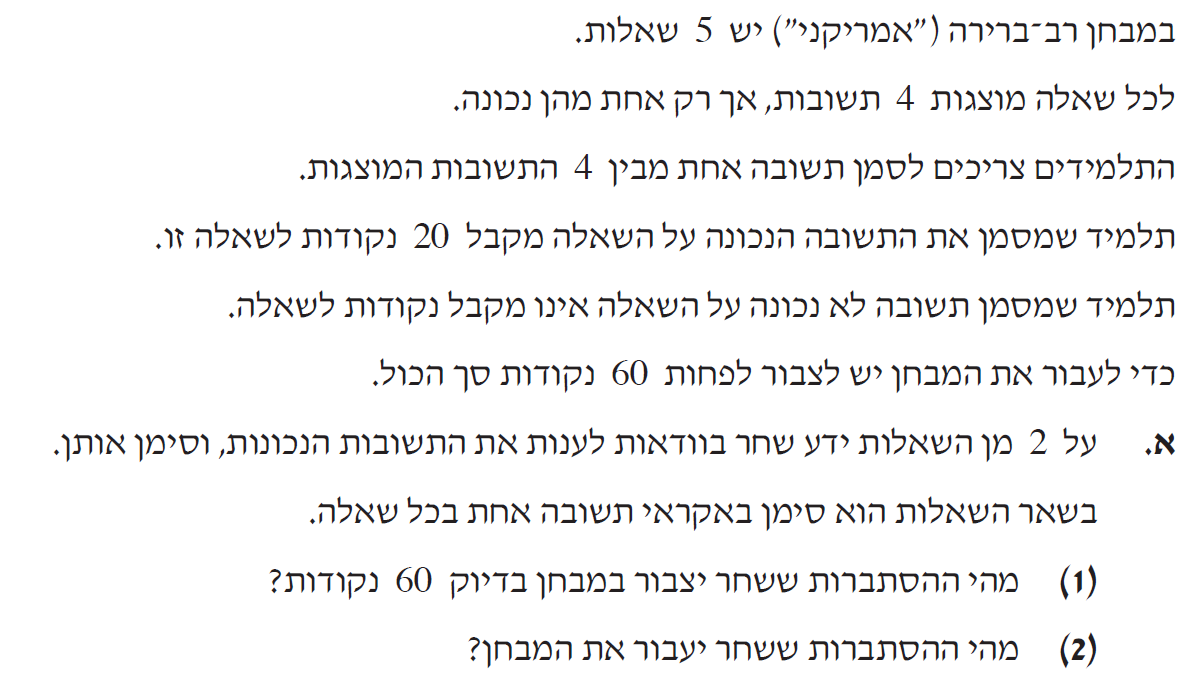
\includegraphics[width=.7\textwidth]{summer-2018b-3a}
\hspace*{-2.2em}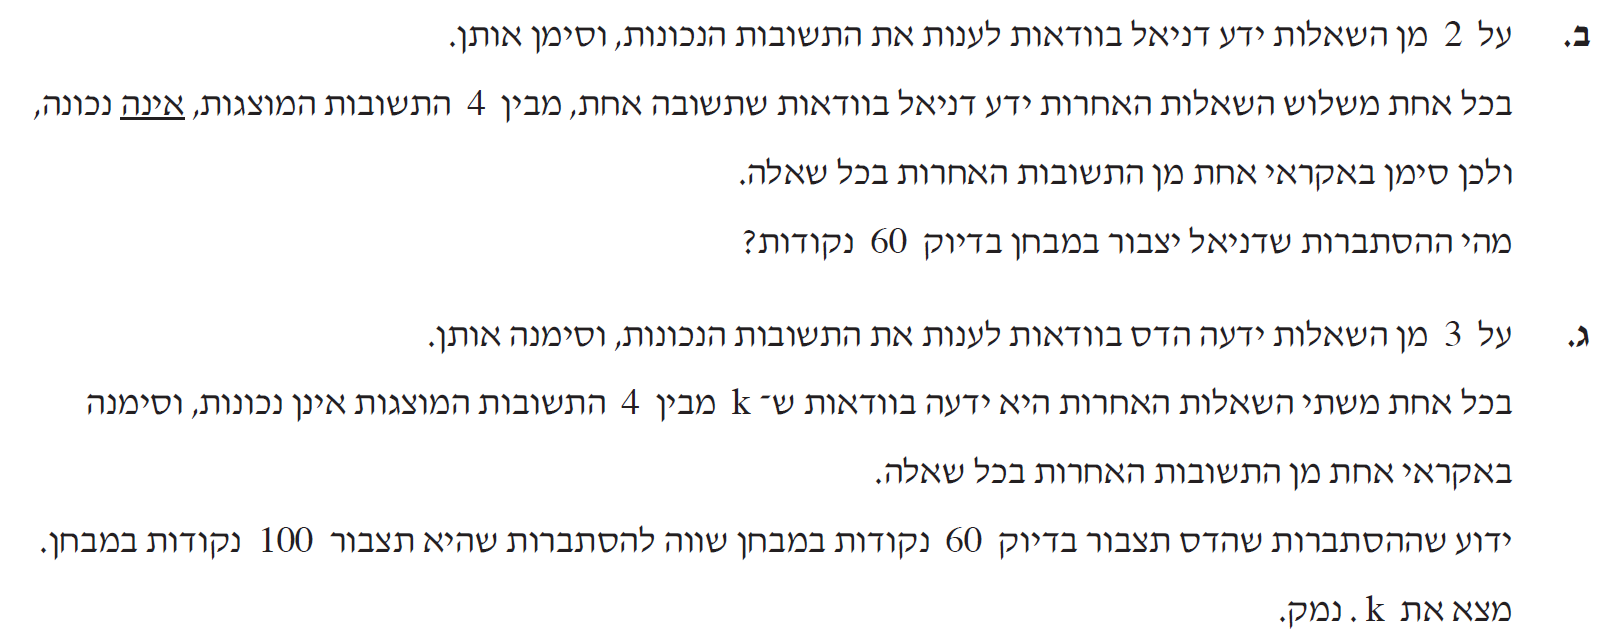
\includegraphics[width=\textwidth]{summer-2018b-3b}
\end{center}

המאורועות הם מספר הנקודות הצברות על ידי התלמידים.

השאלה מתארת הצלחות וכשלונות במתן לתשובות על המבחן ושואלת על מספר ההצלחות והכשלונות. לכן הפתרון ישתמשמ בנוסחת ברנולי.

\textbf{סעיף א}

1. שחר ידע שהוא ענה נכון על שתי שאלות ולכן כדי לקבל ציון
$60$
עליו לענות על בדיוק אחת משלושת השאלות האחרות. ההסתברות לענות נכון על שאלה היא 
$\frac{1}{4}$
ולפי נוסחת ברנולי:
\[
{3 \choose 1}\left(\frac{1}{4}\right)\left(\frac{3}{4}\right)^2=\frac{27}{64}\,.
\]
2. כדי לעבור את המבחן עליו לצבור לפחות שלוש תשובות נכונות. להסתברות מהסעיף הקודם יש להוסיף את ההסתברויות של ארבע וחמש תשובות נכונות:
\[
\frac{27}{64}+{3 \choose 2}\left(\frac{1}{4}\right)^2\left(\frac{3}{4}\right)^1+{3 \choose 3}\left(\frac{1}{4}\right)^3\left(\frac{3}{4}\right)^0=\frac{37}{64}\,.
\]

\newpage

\textbf{סעיף ב}

דניאל צריך לענות נכון על שאלה אחת בדיוק מתוך שלושת השאלות הנותרות. דניאל ידע שתשובה אחת לא נכונה, לכן ההסתברות שהוא ענה נכון על השאלה היא
$\frac{1}{3}$
ולא 
$\frac{1}{4}$
כמו בסעיף הקודם:
\[
{3 \choose 1}\left(\frac{1}{3}\right)\left(\frac{2}{3}\right)^2=\frac{4}{9}\,.
\]
\textbf{סעיף ג}

תהי
$p_k$
ההסתברות שהדס ידעה וודאות ש-%
$k$
מתוך 
$4$
תשובות לא נכונות. ההסתברות שהיא שהיא צריכה לבחור תשובה באופן אקראי היא המשלים
$1-p_k$.
כדי לקבל ציון
$60$
היא צריכה לענות נכון על אפס מתוך שתי השאלות הנוספות וכדי לקבל ציון 
$100$
היא צריכה לענות נכון על כל השאלות הנכונות. נשווה את שתי ההסתברויות המתקבלות מנוסחת ברנולי:
\begin{eqnarray*}
{2 \choose 0}p_k^0(1-p_k)^2 &=& {2 \choose 2}p_k^2(1-p_k)^0\\
(1-p_k)^2 &=& p_k^2\\
p_k&=&\frac{1}{2}\,,
\end{eqnarray*}
כאשר השתמשנו ב-%
${n\choose 0}={n\choose n}=1$
ו-%
$p^0=(1-p)^0=1$.

 ההסתברות שהיא ענתה תשובה נכונה לשאלה אחת היא
$p_k=\displaystyle\frac{1}{4-k}$
ולכן 
$k=2$.

\textbf{פתרון שני}

אם לא היינו מגדירים את הסימון
$p_k$
היינו מקבלים מפישוט השוויון של נוסחאות ברנולי:
\[
\left(\frac{1}{4-k}\right)^2 =\left(1-\frac{1}{4-k}\right)^2=\left(\frac{3-k}{4-k}\right)^2\,.
\]
נכפיל את שני הצדדים של המשוואה ב-%
$(4-k)^2$
ונקבל את המשוואה ריבועית
$k^2-6k+8=0$
שפתרונותיה הם 
$k=2,k=4$.
הפרמטר
$k$
מוגדר כמספר התשובות שהדס יודעת שהן אינן נכונות, ונתון שתשובה אחת נכונה, כך שיש לפסול את הפתרון
$k=4$
ולבחור
$k=2$.

האפשרות השנייה היא לקחת שורש של שני הצדדים ונקבל שתי משוואות:
\begin{eqnarray*}
\frac{1}{4-k}&=&+\frac{3-k}{4-k}\\
\frac{1}{4-k}&=&-\frac{3-k}{4-k}\,.
\end{eqnarray*}
מהמשוואה הראשונה נקבל
$k=2$.
מהמנה של המשוואה השנייה נקבל 
$k=4$
ונפסול אותו כי הוא מאפס את המכנה.

כל הפתרונות מגיעים לתשובה הנכונה אבל בחירה נכונה של סימון וסדר החישובים יכולים להשפוע על פשטות הפתרון.

%%%%%%%%%%%%%%%%%%%%%%%%%%%%%%%%%%%%%%%%%%%%%%%%%%%%%%%%%%%%%%

\newpage

\section{קיץ תשע"ח מועד א}

\begin{center}
\selectlanguage{english}
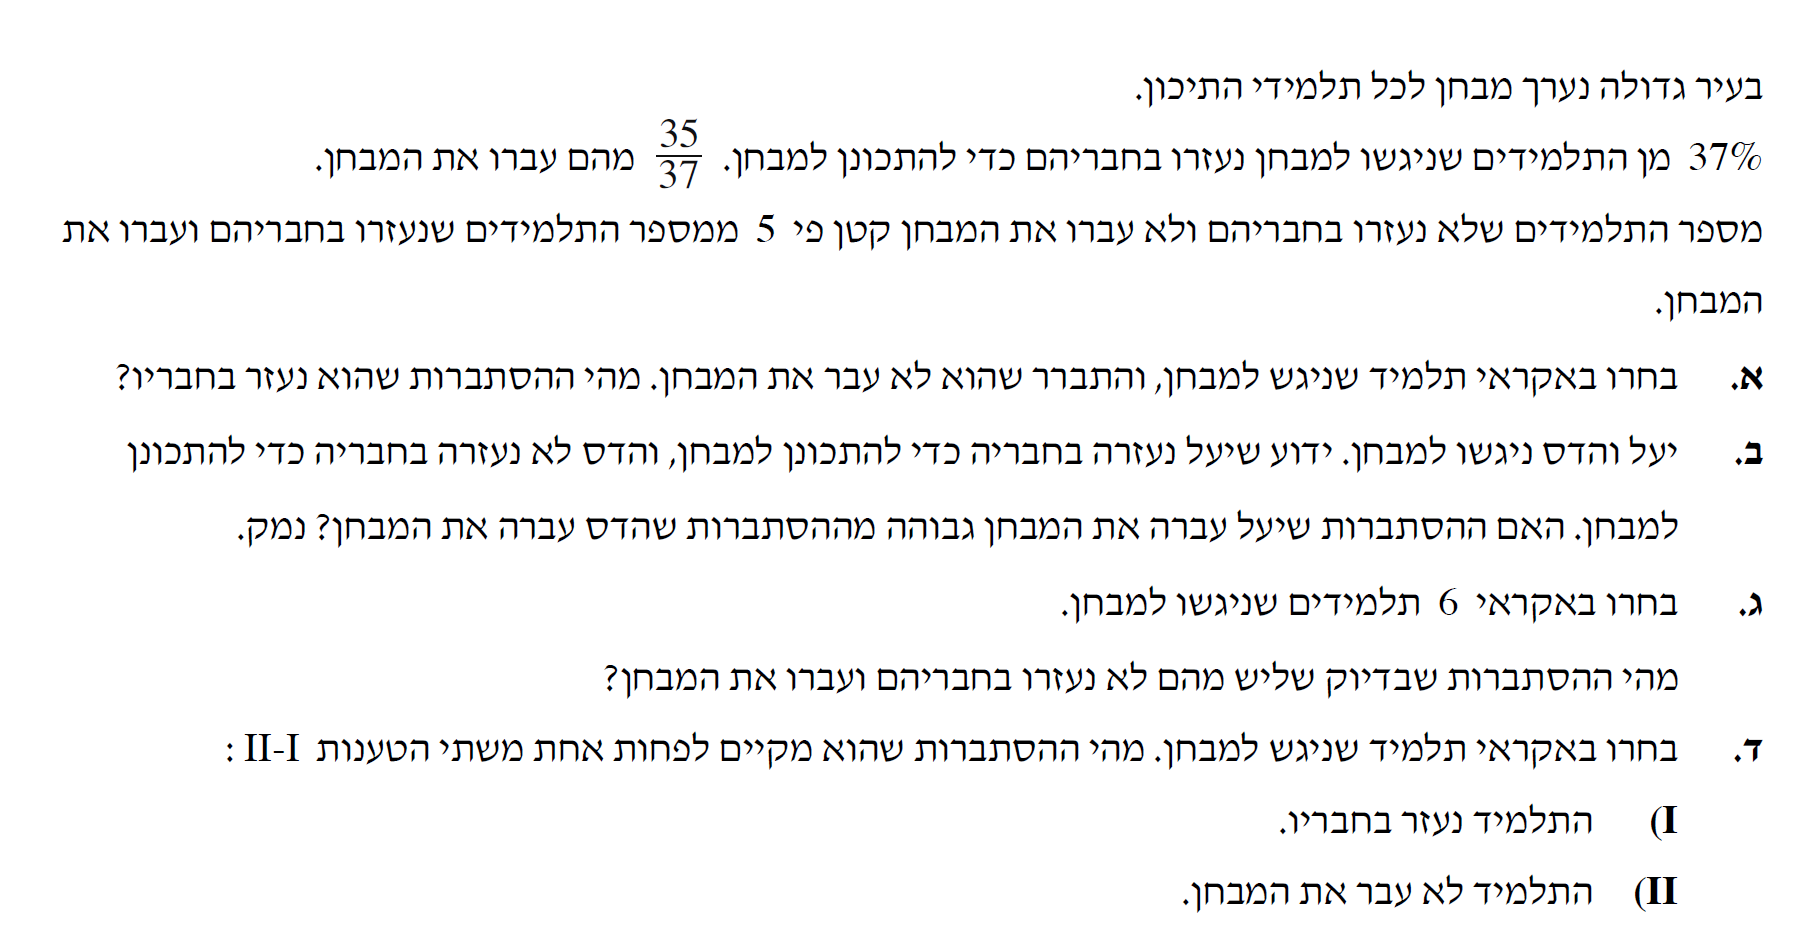
\includegraphics[width=	\textwidth]{summer-2018a-3}
\end{center}

מצאתי שניסוח השאלה מבלבל. כאשר כתוב ש-%
$37\%$
מן התלמידים ניגשו למבחן, הנטייה היא לפרש את זה כ-%
$37$
מתוך
$100$
תלמידים, כאשר אחוז למעשה מבטא יחס:
\[
37\% = \frac{37}{100} = \frac{74}{200} = \frac{18.5}{50} = \cdots\,.
\]
המשפט הבא קובע ש-%
$\frac{35}{37}$
"מהם" עברו את המבחן ואפשר לחשוב שמדובר ב-%
$35$
מתוך
$37$
תלמידים, אולם שוב מדובר ביחס. בשני המקרים יחס הוא הסתברות.

נסמן ב-%
$N$ 
\L{(ne-ezru)}
את התלמידים שנעזרו בחבריהם, וב-%
$A$
\L{(avru)}
את התלמידים שעברו את המבחן. המאורעות מורכבים משתי קבוצות הללו, משלימהם וחיתוכים שלהם, לכן נבחר היעזר בטבלה כדי לייצג את הנתונים. 
לפני שניגש לפתור את השאולות בסעיפים, נמלא את טבלת ההסתברויות לפי המידע הנתון.

\textbf{בניית הטבלה}

נתון ש-%
$P(N)=\frac{37}{100}$.
השימוש במילה
"\textbf{מהם}"
מכוון להסתברות מותנית כך ש:
\[
P(A/N)=\frac{35}{37}
\]
ולכן:
\begin{eqnarray*}
P(A/N) &=& \frac{P(N\cap A)}{P(N)}\\
P(N\cap A) &=& P(A/N)\cdot P(N) = \frac{35}{37}\cdot \frac{37}{100} = \frac{35}{100} = 0.35\,.
\end{eqnarray*}
נשתמש במשלימים להסתברויות ונקבל:
\begin{center}
\selectlanguage{english}
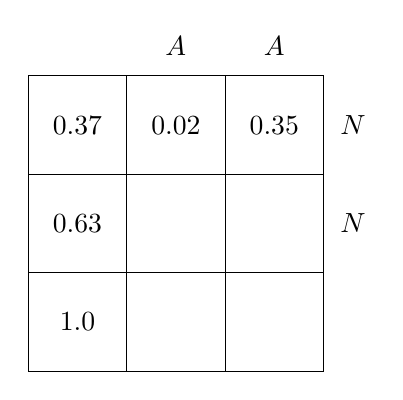
\begin{tikzpicture}[scale=1.25]
\draw (0,0) grid (3,3);
\node at (2.5,3.3) {$\bm{A}$};
\node at (1.5,3.3) {$\bover{A}$};
\node at (3.3,2.5) {$\bm{N}$};
\node at (3.3,1.5) {$\bover{N}$};
\node at (2.5,2.5) {$0.35$};
\node at (0.5,2.5) {$0.37$};
\node at (1.5,2.5) {$0.02$};
\node at (0.5,1.5) {$0.63$};
\node at (0.5,0.5) {$1.0$};
\end{tikzpicture}
\end{center}



בהמשך נתון ש:
\[
P(\overline{N}\cap\overline{A})=\frac{P(N\cap A)}{5}=\frac{0.35}{5}=0.07\,,
\]
וניתן להשלים את הטבלה:
\begin{center}
\selectlanguage{english}
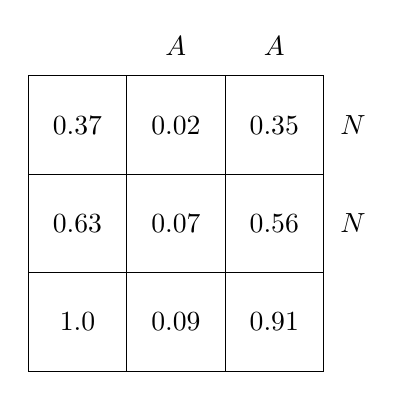
\begin{tikzpicture}[scale=1.25]
\draw (0,0) grid (3,3);
\node at (2.5,3.3) {$\bm{A}$};
\node at (1.5,3.3) {$\bover{A}$};
\node at (3.3,2.5) {$\bm{N}$};
\node at (3.3,1.5) {$\bover{N}$};
\node at (2.5,2.5) {$0.35$};
\node at (0.5,2.5) {$0.37$};
\node at (1.5,2.5) {$0.02$};
\node at (0.5,1.5) {$0.63$};
\node at (0.5,0.5) {$1.0$};
\node at (1.5,0.5) {$0.09$};
\node at (2.5,0.5) {$0.91$};
\node at (1.5,1.5) {$0.07$};
\node at (2.5,1.5) {$0.56$};
\end{tikzpicture}
\end{center}

\smallskip

\textbf{סעיף א}

הניסוח "בחרו 
$\ldots$
תלמיד 
$\ldots$
שלא עבר את המבחן. מה ההסתברות
\textbf{שהוא}
נעזר בחבריו?" מכוון להסתברות מותנית:
\[
P(N/\overline{A})=\frac{P(N\cap \overline{A})}{P(\overline{A})}=\frac{0.02}{0.09}=\frac{2}{9}\,.
\]
\textbf{סעיף ב}

הניסוח
\textbf{"ידוע ש"}
מכוון להסתברות מותנית.

עבור יעל ההסתברות המותנית היא:
\[
P(A/N)=\frac{P(A \cap N)}{P(N)}=\frac{0.35}{0.37}=0.9459\,,
\]
ועבור הדס ההסתברות המותנית היא:
\[
P(A/\overline{N})=\frac{P(A\cap \overline{N})}{P(\overline{N})}=\frac{0.56}{0.63}=0.8889\,.
\]
ליעל הסתברות גבוהה יותר לעבור את המבחן.

\smallskip

\textbf{סעיף ג}

שליש (לא שלושה!) של שש הוא שניים. המילה "בדיוק" מכוון לנוסחת
ברנולי הערך
$P(\overline{N}\cap A)=0.56$
נמצא בטבלה ולפי נוסחה ברנולי ההסתברות היא:
\[
{6 \choose 2}(0.56)^2 (1-0.56)^4=0.1763\,.
\]
\textbf{סעיף ד}

הניסוח
"\textbf{לפחות אחת}"
משתי הטענות
\L{I, II}
אומר שמאורע מורכב משני המאורעות
\L{I, II}
או משניהם. בתרשים להלן שני העגולים המייצגים את שני המאורעות
\L{I, II}
כאשר המאורע "לפחות אחת" מיוצג על ידי כל השטח המקווקו:
\begin{center}
\selectlanguage{english}
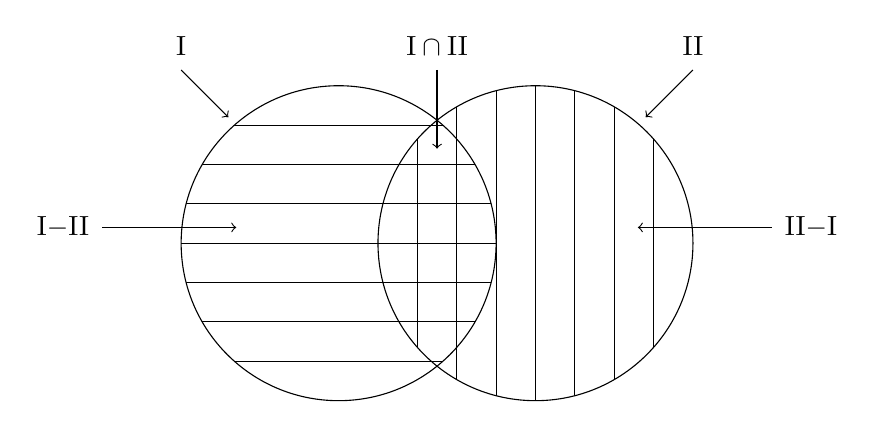
\begin{tikzpicture}
\begin{scope}
\clip[draw] (0,0) circle[radius=2];
\foreach \y in {-1.5,-1,-.5,0,.5,1,1.5}
  \draw (-2,\y) -- (2,\y);
\end{scope}
\begin{scope}
\clip[draw] (2.5,0) circle[radius=2];
\foreach \x in {1,1.5,2,2.5,3,3.5,4}
  \draw (\x,-2) -- (\x,2);
\end{scope}
\node at (-2,2.5) {\textrm{I}};
\node at (4.5,2.5) {\textrm{II}};
\node at (1.25,2.5) {\textrm{I}$\:\cap\:$\textrm{II}};
\node at (-3.5,.2) {\textrm{I$-$II}};
\node at (6,.2) {\textrm{II$-$I}};
\draw[->] (1.25,2.2) -- ++(0,-1);
\draw[->] (-3,.2) -- ++(1.7,0);
\draw[->] (5.5,.2) -- ++(-1.7,0);
\draw[->] (-2,2.2) -- +(.6,-.6);
\draw[->] (4.5,2.2) -- +(-.6,-.6);
\end{tikzpicture}
\end{center}
יש שתי דרכים לחשב את ההסתברות. בדרך הראשונה אנו לוקחים את סכום ההסתברויות של שני המאורעים, ומחסירים את ההסתברות של המאורע המשותף כי ספרנו אותו פעמיים, פעם כחלק מהמאורע
\L{I}
ופעם כחלק מהמאורע
\L{II}:
\[
P(\textrm{I} \cup \textrm{II}) = P(\textrm{I}) + P(\textrm{II}) - P(\textrm{I} \cap \textrm{II})\,.
\]
בדרך השניה אנו סופרים כל חלק מהמאורע השותף בנפרד, כאשר הסימון
\L{I-II}
הוא כל האיברים בקבוצה 
\L{I}
שאינם בקבוצה
\L{II}
ולהיפך:
\[
P(\textrm{I} \cup \textrm{II}) = P(\textrm{I}\:-\:\textrm{II}) + P(\textrm{II}\:-\:\textrm{I}) + P(\textrm{I} \cap \textrm{II})\,.
\]
את ההסתברויות לחישוב ניקח מהטבלה. הדרך הראשונה מופיעה מימין והדרך השניה משמאל:
\begin{center}
\selectlanguage{english}
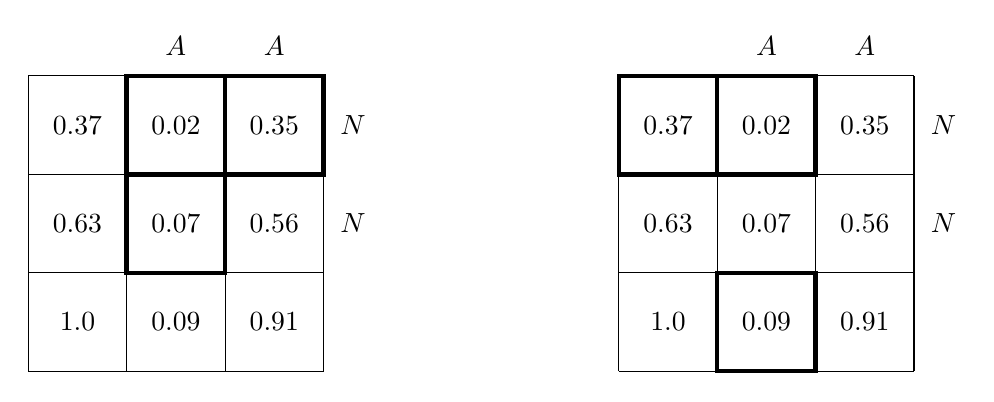
\begin{tikzpicture}[scale=1.25]
\begin{scope}
\draw (0,0) grid (3,3);
\node at (2.5,3.3) {$\bm{A}$};
\node at (1.5,3.3) {$\bover{A}$};
\node at (3.3,2.5) {$\bm{N}$};
\node at (3.3,1.5) {$\bover{N}$};
\node at (2.5,2.5) {$0.35$};
\node at (0.5,2.5) {$0.37$};
\node at (1.5,2.5) {$0.02$};
\node at (0.5,1.5) {$0.63$};
\node at (0.5,0.5) {$1.0$};
\node at (1.5,0.5) {$0.09$};
\node at (2.5,0.5) {$0.91$};
\node at (1.5,1.5) {$0.07$};
\node at (2.5,1.5) {$0.56$};
\draw[ultra thick] (2,2) rectangle +(1,1);
\draw[ultra thick] (1,1) rectangle +(1,1);
\draw[ultra thick] (1,2) rectangle +(1,1);
\end{scope}
\begin{scope}[xshift=6cm]
\draw (0,0) grid (3,3);
\node at (2.5,3.3) {$\bm{A}$};
\node at (1.5,3.3) {$\bover{A}$};
\node at (3.3,2.5) {$\bm{N}$};
\node at (3.3,1.5) {$\bover{N}$};
\node at (2.5,2.5) {$0.35$};
\node at (0.5,2.5) {$0.37$};
\node at (1.5,2.5) {$0.02$};
\node at (0.5,1.5) {$0.63$};
\node at (0.5,0.5) {$1.0$};
\node at (1.5,0.5) {$0.09$};
\node at (2.5,0.5) {$0.91$};
\node at (1.5,1.5) {$0.07$};
\node at (2.5,1.5) {$0.56$};
\draw[ultra thick] (0,2) rectangle +(1,1);
\draw[ultra thick] (1,0) rectangle +(1,1);
\draw[ultra thick] (1,2) rectangle +(1,1);
\end{scope}
\end{tikzpicture}
\end{center}
בשתי הדרכים מקבלים אותה תוצאה:
\begin{eqnarray*}
P(N\cup\overline{A})&=&P(N) + P(\overline{A}) - P(N\cap\overline{A}) = 0.37+0.09-0.02=0.44\\
P(N\cup\overline{A})&=&P(N-\overline{A}) + P(\overline{A}-N) + P(N\cap\overline{A}) = 0.35+0.07+0.02=0.44\,.
\end{eqnarray*}

%%%%%%%%%%%%%%%%%%%%%%%%%%%%%%%%%%%%%%%%%%%%%%%%%%%%%%%%%%%%%

\newpage

\section{חורף תשע"ח}

\begin{center}
\selectlanguage{english}
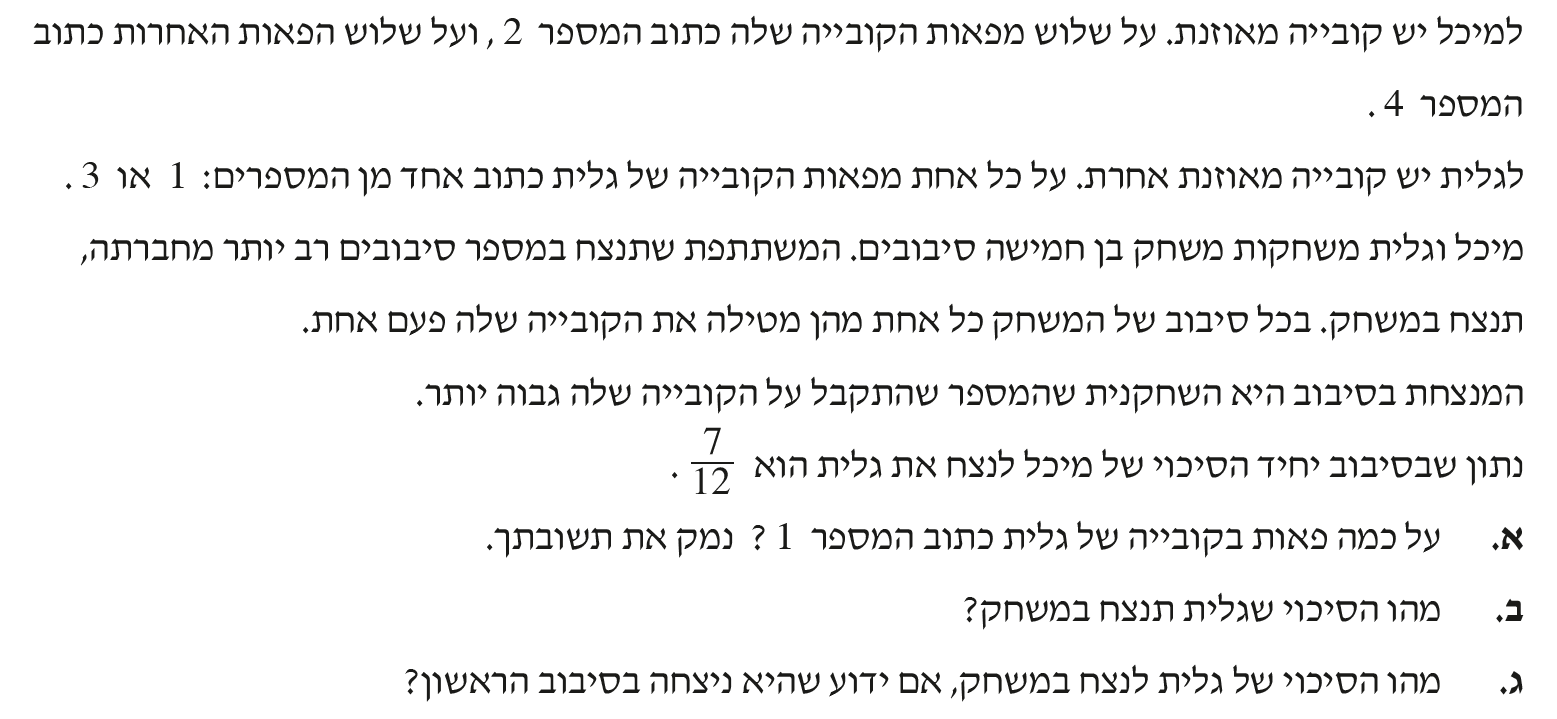
\includegraphics[width=\textwidth]{winter-2018-3}
\end{center}

\textbf{סעיף א}

נסמן ב-%
$n$
את המספר הפאות של הקוביה של גלית שכתוב עליהן
$1$.
מאורע אחד הוא שמיכל תנצח כי היא מטילה 
$4$
בהסתברות
$\frac{3}{6}$
לא משנה מה גלית מטילה. מאורע שני הוא שמיכל תנצח כי היא מטילה 
$2$
בהסתברות
$\frac{3}{6}$
וגלית מטילה
$1$
בהסתברות
$\frac{n}{6}$.
המאורעות זרים זה לזה ולכן:
\begin{eqnarray*}
P(\textrm{\R{מיכל תנצח}}) &=&
\frac{3}{6}\cdot 1 + \frac{3}{6}\cdot \frac{n}{6}=\frac{7}{12}\\
n &=& 1\,.
\end{eqnarray*}
\textbf{סעיף ב}

גלית תנצח אם היא תנצח ב-%
$3,4,5$
סיבובים. נשמתמש בנוסחת ברנולי כדי לקבל את ההסתברות כתלות של ההסתברות של גלית לנצח בסיבוב אחד שהיא המשלים להסתברות שמיכל תנצח
$1-\frac{7}{12}=\frac{5}{12}$:
\[
P(\textrm{\R{גלית תנצח}})={5\choose 3}\left(\frac{5}{12}\right)^3\left(\frac{7}{12}\right)^2+{5\choose 4}\left(\frac{5}{12}\right)^4\left(\frac{7}{12}\right)^1+{5\choose 5}\left(\frac{5}{12}\right)^5\left(\frac{7}{12}\right)^0=0.3466\,.
\]
\textbf{סעיף ג}

הניסוח
\textbf{אם ידוע}
מכוון להסתברות מותנית. נסמן ב-%
$G$
את המאורע שגלית תנצח במשחק וב-%
$R$
את המאורע שהיא תנצח בסיבוב הראשון:
\[
P(G/R) = \frac{P(G \cap R)}{P(R)}\,.
\]
כדי שגלית תנצח במשחק וגם בסיבוב הראשון, היא חייבת לנצח בסיבוב הראשון וגם ב-%
$2$
או
$3$
או
$4$
מהסיבובים הנותרים:
\begin{eqnarray*}
P(G \cap R)&=&\frac{5}{12}\left[{4 \choose 4}\left(\frac{5}{12}\right)^4 \left(\frac{7}{12}\right)^0+
{4 \choose 3}\left(\frac{5}{12}\right)^3 \left(\frac{7}{12}\right)^1+
{4 \choose 2}\left(\frac{5}{12}\right)^2 \left(\frac{7}{12}\right)^2\right]\\
&=&\textstyle\frac{5}{12}\cdot 0.5534\,.
\end{eqnarray*}
כבר חישבנו ש-%
$P(R)=\frac{5}{12}$
ולכן 
$P(G/R)= 0.5534$.

% !TeX root = probability.tex

%%%%%%%%%%%%%%%%%%%%%%%%%%%%%%%%%%%%%%%%%%%%%%%%%%%%%%%%%%%%%

\selectlanguage{hebrew}

\section{קיץ תשע"ז מועד ב}

\begin{center}
\selectlanguage{english}
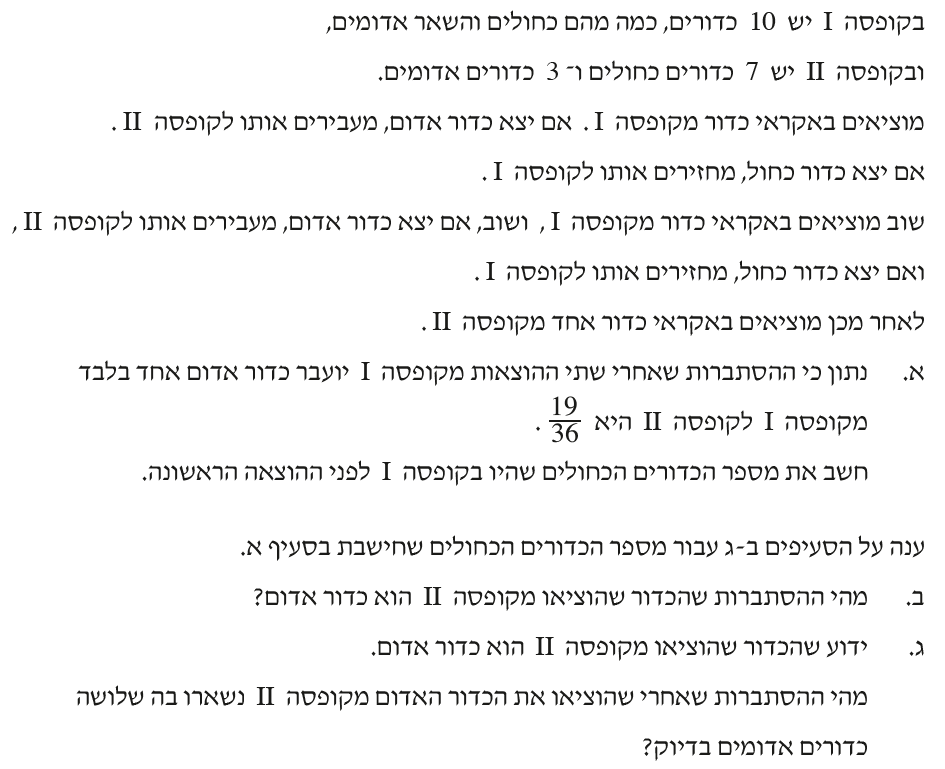
\includegraphics[width=.95\textwidth]{summer-2017b-3}
\end{center}
הניסוח "מוציאים באקראי
$\ldots$
\textbf{ולאחר מכן}
שוב מוציאים באקראי" מכוונן לשימוש בעץ. נסמן ב-%
$b$
את מספר הכדורים הכחולים בקופסה
\L{I}.
בתרשים (בעמוד הבא) בכל צומת רשום שני זוגות של מספרים: למעלה רשום מספר הכדורים האדומים ומספר הכדורים הכחולים בקופסה
\L{I}
ומתחתיו מספר הכדורים האדומים ומספר הכדורים הכחולים בקופסה
\L{II}.
על הקשתות רשום צבע הכדור שנשלף ומתחתיו ההסתברות לשלוף את הצבע. למשל, בקשת הראשונה נשלף כדור אדום וההסתברות היא מספר הכדורים האדומים 
$10-b$
חלקי מספר הכדורים בקופסה
$(10-b)+b=10$.

\begin{figure}
\begin{center}
\begin{tikzpicture}
[grow=right,
level 1/.append style={text width=2cm,level distance=5cm,sibling distance=10em},
level 2/.append style={text width=2cm,level distance=7cm,sibling distance=6em}]
\node[text width=2cm] {(10-b,b)\\(3,7)} % root
child {
  node {(10-b,b)\\(3,7)}
    child {
      node {(10-b,b)\\(3,7)}
      edge from parent node[below] {\R{כחול}}
        node[above,xshift=16mm,yshift=-2mm] {$\frac{b}{10}$}
    }
    child {
      node {(9-b,b)\ *\\(4,7)}
      edge from parent node[above] {\R{אדום}}
        node[below,xshift=16mm,yshift=2mm] {$\frac{10-b}{10}$}
    }
    edge from parent node[below] {\R{כחול}} node[above,xshift=8mm,yshift=0mm] {$\frac{b}{10}$}
}
child { 
  node {(9-b,b)\\(4,7)}
    child {
      node {(9-b,b)\ *\\(4,7)}
      edge from parent node[below] {\R{כחול}}
        node[above,xshift=16mm,yshift=-2mm] {$\frac{b}{9}$}
    }
    child {
      node {(8-b,b)\\(5,7)}
      edge from parent node[above] {\R{אדום}}
        node[below,xshift=16mm,yshift=2mm] {$\frac{9-b}{9}$}
    }
    edge from parent node[above] {\R{אדום}} 
      node[below,xshift=8mm,yshift=0mm] {$\frac{10-b}{10}$}
};
\end{tikzpicture}
\end{center}
\end{figure}

\textbf{סעיף א}

הכוכביות בתרשים מסמנות את שני המסלולים המגיעים למאורע המבוקש 
$R1$:
שנשלף כדור אדום אחד בדיוק מקופסה
\L{I}.
שתי השליפות הן זרות זו לזו ולכן ההסתברות היא סכום ההסתברות לאורך כל אחד מהמסלולים, והסתברות זו נתונה בשאלה:
\[
P(R1)=\frac{10-b}{10}\cdot\frac{b}{9} + \frac{b}{10}\cdot\frac{10-b}{10} = \frac{19}{36}\,.
\]
נפשט ונקבל משוואה ריבועית 
$b^2-10b+25=0$
שיש לה פתרון אחד
$b=5$.


\textbf{סעיף ב}

מהמידע הרשום בצד הימיני של התרשים אפשר לראות שמספר הכדורים האדומים שנמצאים בקופסה
\L{II}
הם:
$5,4,4,7$.
נסכם את ההסתברויות של המאורע
$P(R2$,
לשלוף כדור אדום מקופסה
\L{II},
לאורך כל אחד מהמסלולים כאשר קודם נציב 
$b=5$
שמצאנו לעיל:
\[
\begin{array}{rcl}
P(R2)&=&\displaystyle\left(\frac{5}{10}\cdot\frac{4}{9}\right)\left(\frac{5}{12}\right)+
\left(\frac{5}{10}\cdot\frac{5}{9}\right)\left(\frac{4}{11}\right)+\\
&&\displaystyle\left(\frac{5}{10}\cdot\frac{5}{10}\right)\left(\frac{4}{11}\right)+
\left(\frac{5}{10}\cdot\frac{5}{10}\right)\left(\frac{3}{10}\right)
=0.3595\,.
\end{array}
\]

\textbf{סעיף ג}

הניסוח
"\textbf{ידוע ש-}"
מכוון להסתברות מותנית. המאורע החדש הוא
$P(R3)$:
נשארו שלושה כדורים אדומים בקופסה 
\L{II}:
\[
P(R3/R2)=\frac{P(R3\cap R2)}{P(R2)}\,.
\]
את
$P(R2)$
חישבנו בסעיף הקודם.

נשארו שלושה כדורים אדומים רק אם היו אברעה כדורים אדומים לפני הבחירה, מאורע 
$R4$.
ההסתברות 
$P(R4)$
למעשה נתונה
$\frac{19}{36}$,
והיא ההסתברות להגיע לאחד המצבים המסומנים בכוכבית. מכאן שההסתברות של 
$P(R3)$
היא ההסתברות להגיע לאחד מהמצבים כפול ההסתברות לשלוף כדור אדום במצב זה:
\[
P(R3)=P(R4)\cdot \textstyle\frac{4}{11}\,.
\]
ההסתברות המותנית הדרושה היא:
\[
P(R3/R2)=\frac{\frac{19}{36}\cdot\frac{4}{11}}{0.3595}=0.53385\,.
\]

%%%%%%%%%%%%%%%%%%%%%%%%%%%%%%%%%%%%%%%%%%%%%%%%%%%%%%%%%%%%%%%%%%%

\section{קיץ תשע"ז מועד א}

\begin{center}
\selectlanguage{english}
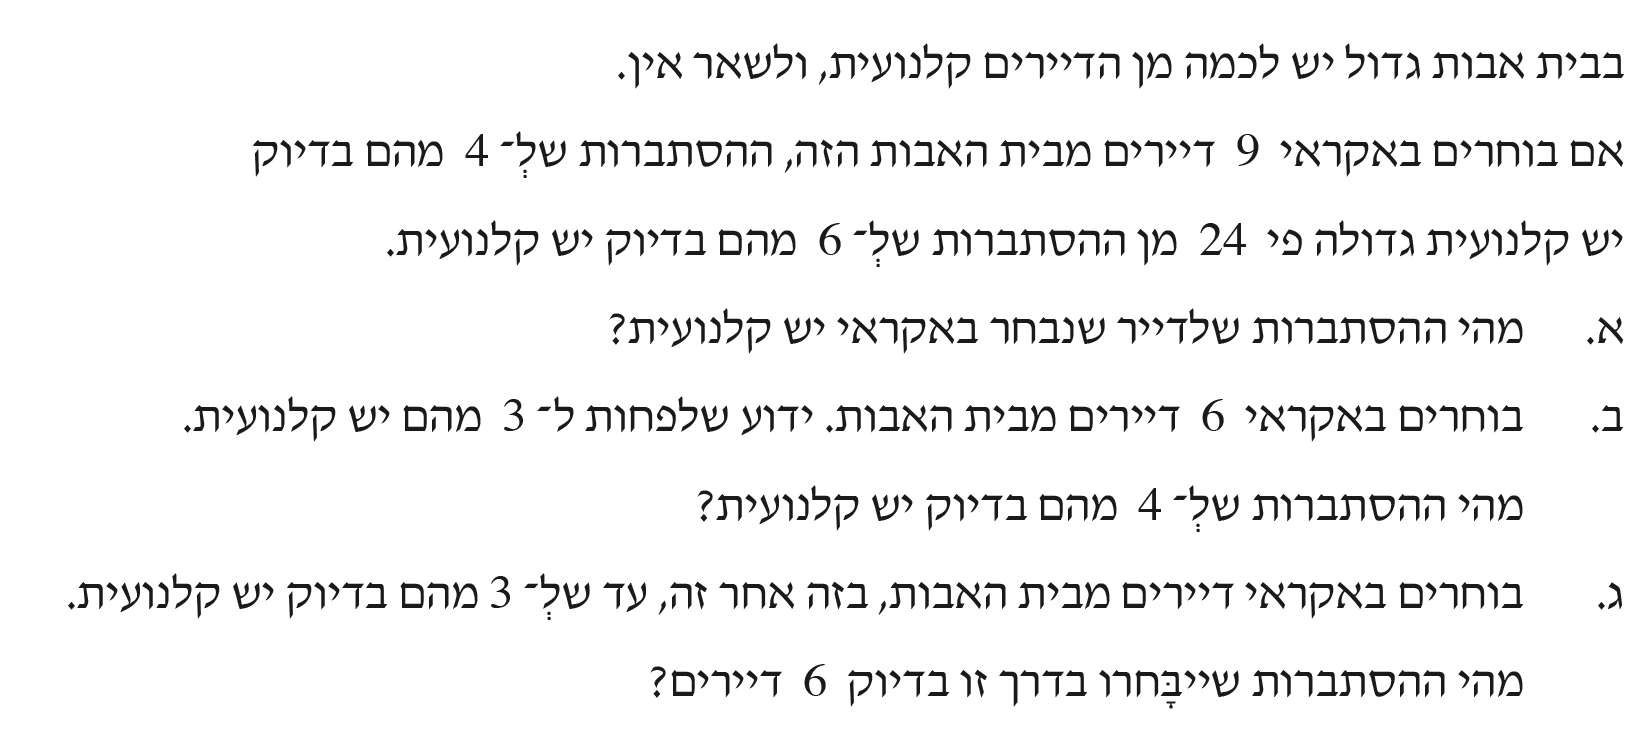
\includegraphics[width=.95\textwidth]{summer-2017a-3}
\end{center}

\textbf{סעיף א}

נסמן ב-%
$D$
את המאורע "לדייר יש קלנועית" ונסמן
$P(D)=p$.
לפי ניסוח השאלה הצלחה היא בחירת דייר עם קלנועית ונמסר מידע על "בדיוק" מספר ההצלחות, ולכן נשמתש בנוסחת ברנולי לכדי לקבל משוואה במשתנה 
$p$:
\begin{eqnarray*}
{9\choose 4} p^4 (1-p)^5&=&24 {9\choose 6} p^6 (1-p)^3\\
\frac{1}{4}(1-p)^2&=&\frac{24}{6}p^2\\
15p^2+2p-1&=&0\\
p&=&\frac{1}{5}=0.2\,,
\end{eqnarray*}
כאשר השורש 
$-\frac{1}{3}$
אינו יכול להיות פתרון כי הסתברות חייבת גדול או שווה לאפס.

\textbf{סעיף ב}

נסמן ב-%
$N$
את המאורע של "מספר הדיירים שיש להם קלנועית". הניסוח
"\textbf{ידוע ש-}"
מכוון להסתברות מותנית:
\[
P(N=4/N\ge3) = \frac{P(N=4\cap N\ge 3)}{P(N\ge 3)}\,.
\]
כאשר קבוצה אחת בחיתוך היא תת-קבוצה של השנייה, אפשר לפשט את החיתוך ולהשתמש רק בקבוצה הקטנה יותר. ברור שאם 
$N$
גדול או שווה ל-%
$3$
\textbf{וגם}
$N$
שווה ל-%
$4$
אז
$N$
שווה ל-%
$4$:
\[
P(N=4/N\ge3) =\frac{P(N=4)}{P(N\ge 3)}\,.
\]
לפי נוסחת ברנולי:
\[
P(N=4)={6\choose 4} 0.2^4 (1-0.2)^2= 0.01536\,.
\]
המונה
$P(N\ge 3)$
אפשר לחשב בשתי דרכים. בצורה ישירה:
\begin{eqnarray*}
P(N\ge 3)&=&{6\choose 3}0.2^3(1-0.2)^3+{6\choose 4}0.2^4(1-0.2)^2+\\
&&{6 \choose 5} 0.2^5(1-0.2)^1+ {6 \choose 6} 0.2^6(1-0.2)^0=0.099\,,
\end{eqnarray*}
או לפי המשלים:
\begin{eqnarray*}
P(N\ge 3)=1-P(N<3)&=&
1-0.2^0(1-0.2)^6-{6\choose 1}0.2^1(1-0.2)^5 -\\
&&{6 \choose 2} 0.2^2(1-0.2)^4=0.099\,.
\end{eqnarray*}
התשובה לשאלה היא:
\[
P(N=4/N\ge3) =\displaystyle\frac{P(N=4)}{P(N\ge 3)}=\displaystyle\frac{0.01536}{0.099}=0.15534\,.
\]
\textbf{סעיף ג}

הניסוח 
"\textbf{עד ש}"
אומר שהבחירה 
\textbf{האחרונה} 
תהיה "הצלחה" ושיהיו שתי "הצלחות" בחמשת הבחירות הקודמות. נסמן הצלחה ב-%
$+$
וכישלון ב-%
$-$
ונסדר את הדרישה בשאלה בשורה:
\[
\overbrace{\pm\;\pm\;\pm\;\pm\;\pm}^{2/5}\quad\quad \overbrace{+}^{1/1}
\]
התשובה מתקבלת מנוסחת ברנולי לבחירות הראשונות כפול ההסתברות
$p$
לבחירה האחרונה:
\[
\left[{5\choose 2}0.2^2 (1-.02)^3\right]\cdot 0.2=0.04096\,.
\]

%%%%%%%%%%%%%%%%%%%%%%%%%%%%%%%%%%%%%%%%%%%%%%%%%%%%%%%%%%%%%

\section{חורף תשע"ז}

\begin{center}
\selectlanguage{english}
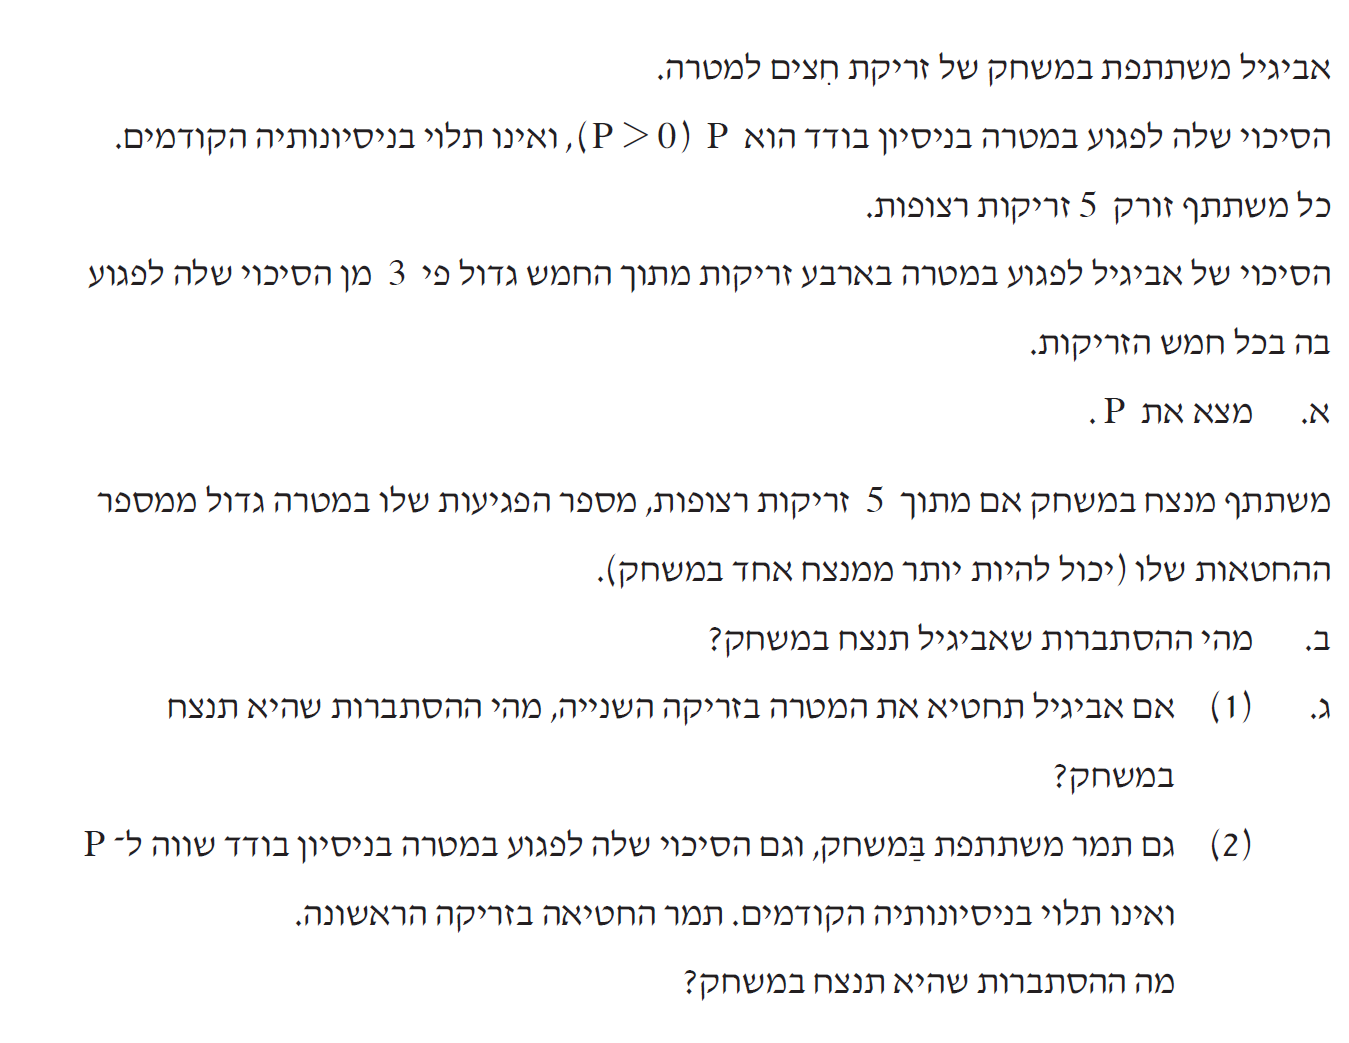
\includegraphics[width=.95\textwidth]{winter-2017-3.png}
\end{center}

\textbf{סעיף א}

נסמן ב-%
$A$
את המאורע "אביגיל פוגעת" ונסמן
$P(A)=p$.
לפי ניסוח השאלה הצלחה היא פגיעה במטרה ונמסר מידע על מספר ההצלחות, ולכן נשמתש בנוסחת ברנולי לכדי לקבל משוואה במשתנה 
$p$:
\begin{eqnarray*}
{5 \choose 4} p^4(1-p)^1 &=& 3{5\choose 5}p^5(1-p)^0\\
5(1-p) &=& 3p\\
p&=&\frac{5}{8}\,.
\end{eqnarray*}

\textbf{סעיף ב}

נסמן ב-%
$N5$
את מספר הפגיעות של אביגיל מתוך חמש זריקות. ניצחון שלה היא 
$N5\geq 3$
וההסתברות היא:
\[
P(N5\geq 3)=
{5 \choose 3}p^3(1-p)^2 + {5 \choose 4}p^4(1-p)^1 + {5 \choose 5}p^5(1-p)^0.
\]
נציב
$p=\displaystyle\frac{5}{8}$
ונקבל
$0.7248$.

\textbf{סעיף ג (1)}

לדעתי ניסוח השאלה לא ברור. אני פירשתי אותה כך: מה ההסתברות של
\textbf{המאורע}
"אביגיל מחטיאה בזריקה השנייה ופוגעת בשלוש או ארבע מהזריקות האחרות"? כותב הבחינה התכוון להסתברות מותנית: "%
\textbf{אם ידוע}
שאביגיל החטיאה בזריקה השנייה, מה ההסתברות שהיא פוגעת בשלוש או ארבע מהזריקות האחרות"?

נסמן ב-%
$T2$
את המאורע שאביגיל מחטיאה בזריקה השנייה, ונסמן ב-%
$N4$
את מספר הפגיעות שלה מתוך ארבע זריקות. ההסתברות המותנית היא:
\[
P(N4\geq 3/T2) = \frac{P(N4\geq 3\cap T2)}{P(T2)}\,.
\]
הזריקות לא תלויות אחת בשנייה ולכן:
\[
P(N4\geq 3/T2) = \frac{P(N4\geq 3)\cdot P(T2)}{P(T2)}=P(N4\geq 3)\,,
\]
ולפי נוסחת ברנולי:
\[
P(N4\geq 3/T2) =P(N4\geq 3)=
{4\choose 4}\left(\frac{5}{8}\right)^4 \left(\frac{3}{6}\right)^0 +{4\choose 3}\left(\frac{5}{8}\right)^3\left(\frac{3}{8}\right)^1 = 0.5188\,.
\]

\textbf{סעיף ג (2)}

ההסתברות של תמר לפגוע זהה להסתברות של אביגיל לפגוע ולכן ניתן להשמתמש בתוצאות שכבר חישבנו. גם לא משנה איזו זריקה החטיאה כי הזריקות בלתי תלויות, ולכן לפי סעיף ג (1) ההסתברות של תמר לנצח היא גם
$0.5188$.

% !TeX root = probability.tex

%%%%%%%%%%%%%%%%%%%%%%%%%%%%%%%%%%%%%%%%%%%%%%%%%%%%%%%%%%%%%

\section{קיץ תשע"ו מועד ב}

\begin{center}
\selectlanguage{english}
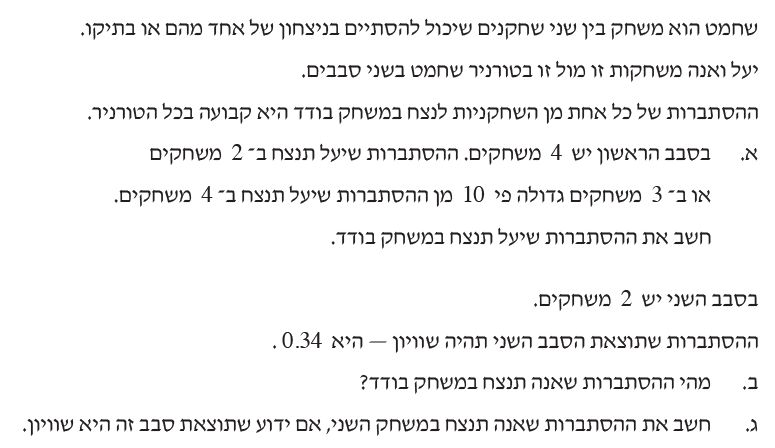
\includegraphics[width=.86\textwidth]{summer-2016b-3}
\end{center}

\textbf{סעיף א}

נסמן את המאורע "יעל תנצח במשחק בודד" ב-%
$Y$ \L{(Yael)}
ונסמן
$y=P(Y)$.
הצלחה מוגדרת על ידי ניצחונות של יעל והשאלה מספקת מידע על מספרי ההצלחות ולכן נשמתמש בנוסחת ברנולי:
\begin{eqnarray*}
{4 \choose 2}y^2(1-y)^2 + {4\choose 3}y^3(1-y) &=& 10\cdot {4\choose 4}y^4(1-y)^0\\
8y^2+8y-6&=&0\\
y&=&\frac{1}{2}\,,
\end{eqnarray*}
ונתעלם מהשורש השני 
$-\frac{3}{2}$
כי הסתברות לא יכולה להיות שלילי.

\textbf{סעיף ב}

נסמן את המאורע "אנה תנצח במשחק בודד" ב-%
$A$ \L{(Anna)}
ונסמן
$a=P(A)$.

נסמן ב-%
$S$ \L{(shivyon)}
את המאורע שתוצאת הסבב השני תהיה תיקו. האפשרויות לקבל שוויון הן ניצחון אחד לאנה וליעל בהסתברות 
$ya+ay$,
או תיקו בשני המשחקים בהסתברות
$(1-(y+a))^2$
כי ההסתברות לתיקו במשחק אחד היא המשלים לסכום ההסתברויות שאחת מהן תנצח. נציב
$y=\frac{1}{2}$
והמידע ש-%
$P(S)=0.34$
ונקבל:
\begin{eqnarray*}
{2 \choose 1}ya + (1-(y+a))^2 &=&P(S)= 0.34\\
a + (\textstyle\frac{1}{2}-a)^2&=&0.34\\
a&=&0.3\,,
\end{eqnarray*}
כאשר נתעלם מהשורש
$-0.3$
כי הסתברות לא יכולה להיות שלילית.

\textbf{סעיף ג}

נסמן את המאורע "אנה תנצח במשחק השני" ב-%
$A2$.

הניסוח
"\textbf{אם ידוע ש-}"
מכוון להסתברות מותנית:
\begin{eqnarray*}
P(A2/S) &=& \frac{P(A2\:\cap\;S)}{P(S)}\\
&=&\frac{ya}{P(S)}=\frac{0.5\cdot 0.3}{0.34}=0.4412\,.
\end{eqnarray*}

ההסתברות לשיוון בסבב השני נתונה. אם אנה תנצח במשחק השני, יהיה שוויון רק אם גם יעל תנצח במשחק הראשון:
\[
\frac{ya}{.34}=\frac{0.5\cdot 0.3}{.34}=0.4412\,.
\]
שימו לב שאם יש שיוון ואנה מנצחת במשחק הראשון, יעל חייבת לנצח במשחק הראשון ולכם המנה היא 
$ya$.

%%%%%%%%%%%%%%%%%%%%%%%%%%%%%%%%%%%%%%%%%%%%%%%%%%%%%%%%%%%%%%

\newpage

\section{קיץ תשע"ו מועד א}

\begin{center}
\selectlanguage{english}
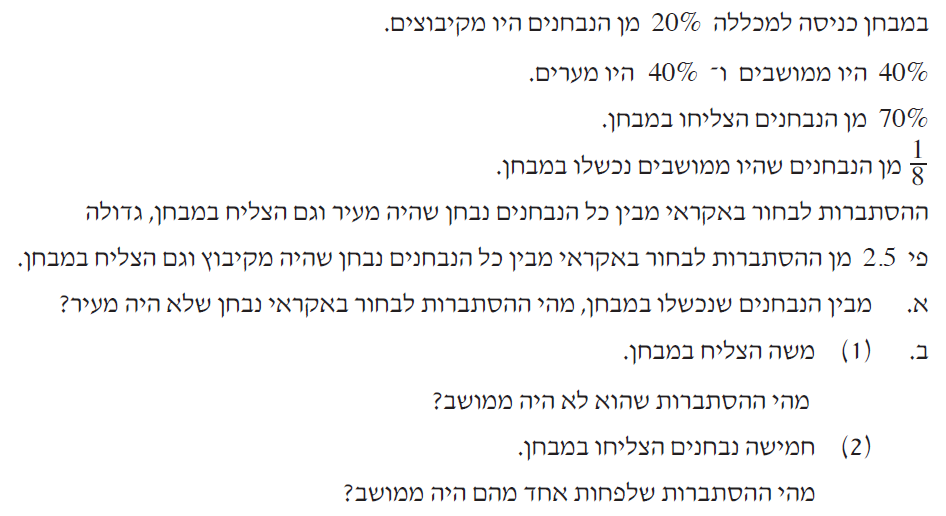
\includegraphics[width=.95\textwidth]{summer-2016a-3}
\end{center}

נסמן את המאורעות השונים בשאלה.
\begin{itemize}
\item $S$ \L{(success)}
הנבחנים שהצליחו.
\item $K$ \L{(kibbutz)} 
נבחנים מקיבוצים.
\item $M$ \L{(moshav)}
נבחנים ממושבים.
\item $E$ \L{(eer)}
נבחנים מערים.
\end{itemize}
ההסתברויות של המאורעות הללו נתונות:
\[
P(K)=0.20,\;P(M)=0.40,\;P(E)=0.40,\;P(S)=0.70\,.
\]
בשאלה שני סוגים של קבוצות: הצלחת הנבחנים ומקום המגורים של הנבחנים ולכן נשתמש בטבלה:
\begin{center}
\selectlanguage{english}
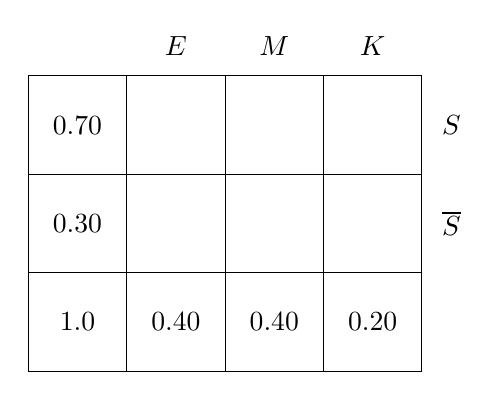
\begin{tikzpicture}[scale=1.25]
\draw (0,0) grid (4,3);
\node at (3.5,3.3) {$K$};
\node at (2.5,3.3) {$M$};
\node at (1.5,3.3) {$E$};
\node at (4.3,2.5) {$S$};
\node at (4.3,1.5) {$\overline{S}$};

\node at (0.5,2.5) {$0.70$};
\node at (0.5,1.5) {$0.30$};
\node at (0.5,0.5) {$1.0$};

%\node at (1.5,2.5) {$0.25$};
%\node at (1.5,1.5) {$0.15$};
\node at (1.5,0.5) {$0.40$};

%\node at (2.5,2.5) {$0.35$};
%\node at (2.5,1.5) {$0.05$};
\node at (2.5,0.5) {$0.40$};

%\node at (3.5,2.5) {$0.10$};
%\node at (3.5,1.5) {$0.10$};
\node at (3.5,0.5) {$0.20$};
\end{tikzpicture}
\end{center}
מידע נוסף שניתן הוא "%
$\frac{1}{8}$
\textbf{מן הנבחנים}
שהיו ממושבים נכשלו במבחן", כאשר הניסוח מכוון להסתברות מותנית. נחשב:
\begin{eqnarray*}
P(\overline{S}/M)&=&P(\overline{S}\cap M) / P(M)\\
P(\overline{S}\cap M)&=&P(\overline{S}/M)\cdot P(M)=\frac{1}{8}\cdot 0.40=0.05\,.
\end{eqnarray*}
הנתון האחרון מתקבל מהפסקאות "ההסתברות לבחור באקראי
\textbf{מבין כל}
הנבחנים נבחן שהיה ב-%
$\cdots$
\textbf{וגם}
הצליח במבחן". הניסוח מכוון לחיתוך הסתברויות, ולכן הנתון הוא
$P(E\cap S)=2.5\cdot P(K\cap S)$.

נחשב את 
$P(S)=0.70$
על ידי סיכום ההסתברויות של המצליחים במבחן בכל מקום מגורים:
\begin{eqnarray*}
P(S)&=&P(K\cap S)+P(M \cap S) + P(K\cap E)\\
0.70&=&P(K\cap S)+ 0.35 + 2.5\cdot P(K\cap S)\\
P(K\cap S)&=&0.10\\
P(E\cap S)&=&0.25\,.
\end{eqnarray*}
נשלים את הטבלה:
\begin{center}
\selectlanguage{english}
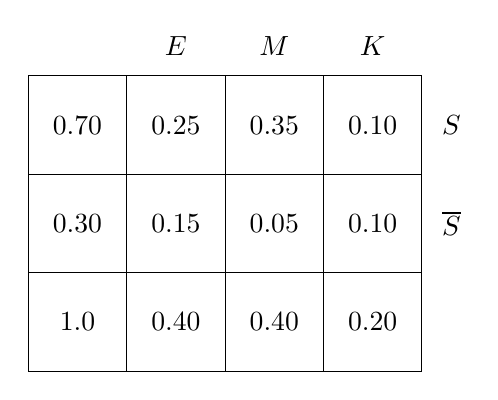
\begin{tikzpicture}[scale=1.25]
\draw (0,0) grid (4,3);
\node at (3.5,3.3) {$K$};
\node at (2.5,3.3) {$M$};
\node at (1.5,3.3) {$E$};
\node at (4.3,2.5) {$S$};
\node at (4.3,1.5) {$\overline{S}$};

\node at (0.5,2.5) {$0.70$};
\node at (0.5,1.5) {$0.30$};
\node at (0.5,0.5) {$1.0$};

\node at (1.5,2.5) {$0.25$};
\node at (1.5,1.5) {$0.15$};
\node at (1.5,0.5) {$0.40$};

\node at (2.5,2.5) {$0.35$};
\node at (2.5,1.5) {$0.05$};
\node at (2.5,0.5) {$0.40$};

\node at (3.5,2.5) {$0.10$};
\node at (3.5,1.5) {$0.10$};
\node at (3.5,0.5) {$0.20$};
\end{tikzpicture}
\end{center}
\textbf{סעיף א}

לפי הנוסחה להסתברות מותנית:
\[
P(\overline{E}/\overline{S})=P((K\cup M)/\overline{S}) = \frac{P(K\cap \overline{S})+P(M\cap \overline{S})}{P(\overline{S})}=\frac{0.10+0.05}{0.30}=\frac{1}{2}\,.
\]
\textbf{(1) סעיף ב}

לפי הנוסחה להסתברות מותנית:
\[
P(\overline{M}/S)=P((K\cup E)/S) = \frac{P(K\cap S)+P(E\cap S)}{P(S)}=\frac{0.10+0.25}{0.70}=\frac{1}{2}\,.
\]
\textbf{(2) סעיף ב}

"לפחות אחד ממושב" הוא המשלים ל-"כולם לא מהמושב" ולפי נוסחת ברנולי:
\[
1-P(\overline{M}/S)^5=1-\left(\frac{1}{2}\right)^2=\frac{31}{32}\,.
\]

%%%%%%%%%%%%%%%%%%%%%%%%%%%%%%%%%%%%%%%%%%%%%%%%%%%%%%%%%%%%

\section{חורף תשע"ו}

\begin{center}
\selectlanguage{english}
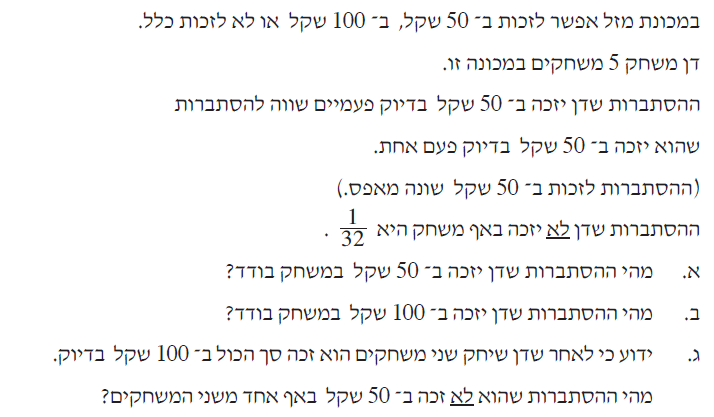
\includegraphics[width=.85\textwidth]{winter-2016-3}
\end{center}

המאורעות הם סכומי הכסף שדן זכה 
$0,50,100$.
נסמן ב-%
$P(n)$
את ההסתברות שדן זכה ב-%
$n$.

\textbf{סעיף א}

הניסוחים "אף אחד" ו-"בדיוק" מכוונים לנוסחת ברנולי. ההסתברות שדן לא זכה (בסכום חיובי) באף אחד מחמישת המשחקים היא 
$P(0)^5=\frac{1}{32}$
ולכן 
$P(0)=\frac{1}{2}$.
לפי המידע הנתון:
\begin{eqnarray*}
{5\choose 2} P(50)^2 (1-P(50))^3 &=& {5\choose 1} P(50) (1-P(50))^4\\
10P(50)&=&5(1-P(50))\\
P(50)&=&\frac{1}{3}\,.
\end{eqnarray*}

\textbf{סעיף ב}

לפי ההסתברות המשלימה:
$P(100) = 1 - P(0) - P(50) = 1-\frac{1}{2}-\frac{1}{3}=\frac{1}{6}$.



\textbf{סעיף ג}

נסמן ב-%
$M2$
את המאורע שדן זכה ב-%
$100$
בשני משחקים ונסמן ב-%
$\overline{50}$
את המאורע שדן לא זכה ב-%
$50$.
הניסוח
"\textbf{ידוע כי}"
מכוון להסתברות מותנית:
\[
P(\overline{50}/M2)=\frac{P(\overline{50}\cap M2)}{P(M2)}
\]
המשחקים מתרחשים אחד אחרי השני ולא לתלויים אחד בשני ולכן ניתן להציג את ההסתברויות בעץ (בעמוד הבא). בסוף כל מסלול רשום המאורעות 
$M2,\overline{50}$
שמתקיימים. ההסתברות המותנית היא:
\[
\frac{\frac{1}{2}\cdot\frac{1}{6} + \frac{1}{6}\cdot \frac{1}{2}}{\frac{1}{2}\cdot\frac{1}{6} + \frac{1}{3}\cdot \frac{1}{3}+ \frac{1}{6}\cdot \frac{1}{2}}  =  \frac{\frac{1}{6}}{\frac{5}{18}}=\frac{3}{5}\,.
\]

\begin{center}
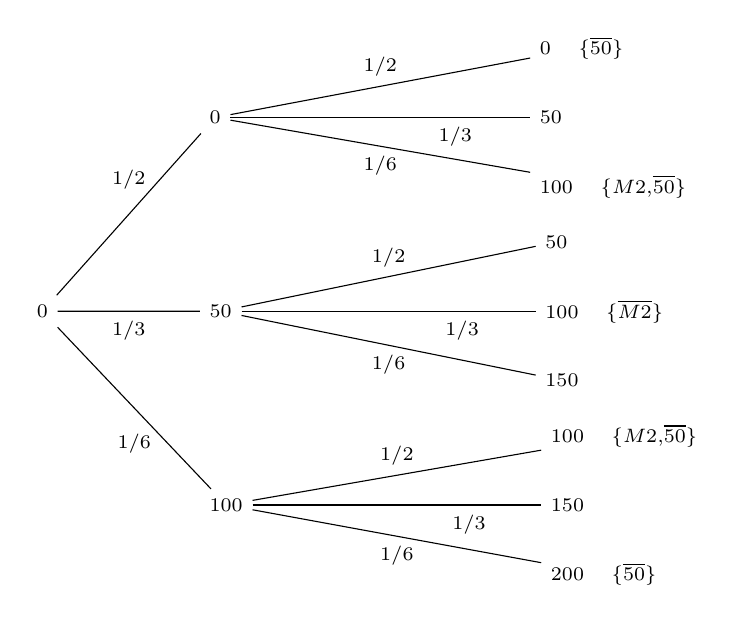
\begin{tikzpicture}
[grow=right,
level 1/.append style={level distance=2cm,
                       sibling distance=7em},
level 2/.append style={level distance=4cm,
                       sibling distance=2.5em}]
\node[left] {$\scriptstyle 0$} % root
child {
  node[right] {$\scriptstyle 100$}
    child {
      node[right] {$\scriptstyle 200\quad \{\overline{50}\}$}
      edge from parent node[below] {$\scriptstyle 1/6$}
    }
    child {
      node[right] {$\scriptstyle 150$}
      edge from parent node[below,near end] {$\scriptstyle 1/3$}
    }
    child {
      node[right] {$\scriptstyle 100\quad \{M2,\overline{50}\}$}
      edge from parent node[above] {$\scriptstyle 1/2$}
    }
    edge from parent node[below,yshift=-2mm] {$\scriptstyle 1/6$}
}
child {
  node[right] {$\scriptstyle 50$}
    child {
      node[right] {$\scriptstyle 150$}
      edge from parent node[below] {$\scriptstyle 1/6$}
    }
    child {
      node[right] {$\scriptstyle 100\quad \{\overline{M2}\}$}
      edge from parent node[below,near end] {$\scriptstyle 1/3$}
    }
    child {
      node[right] {$\scriptstyle 50$}
      edge from parent node[above] {$\scriptstyle 1/2$}
    }
    edge from parent node[below] {$\scriptstyle 1/3$}
}
child {
  node[right] {$\scriptstyle 0$}
    child {
      node[right] {$\scriptstyle 100\quad \{M2,\overline{50}\}$}
      edge from parent node[below] {$\scriptstyle 1/6$}
    }
    child {
      node[right] {$\scriptstyle 50$}
      edge from parent node[below,near end] {$\scriptstyle 1/3$}
    }
    child {
      node[right] {$\scriptstyle 0\quad \{\overline{50}\}$}
      edge from parent node[above] {$\scriptstyle 1/2$}
    }
    edge from parent node[above,yshift=2mm] {$\scriptstyle 1/2$}
}
;
\end{tikzpicture}
\end{center}


% !TeX root = probability.tex

%%%%%%%%%%%%%%%%%%%%%%%%%%%%%%%%%%%%%%%%%%%%%%%%%%%%%%%%%%%%%

%%%%%%%%%%%%%%%%%%%%%%%%%%%%%%%%%%%%%%%%%%%%%%%%%%%%%%%%%%%%%%

\section{קיץ תשע"ה מועד ב}

\begin{center}
\selectlanguage{english}
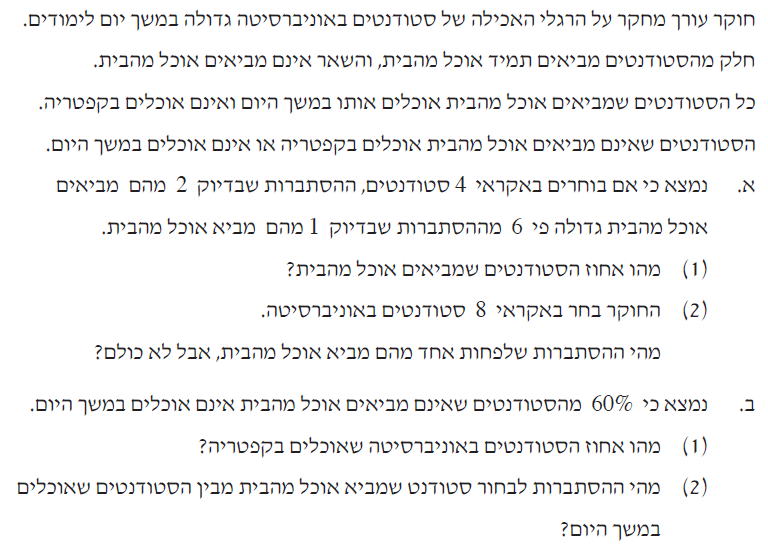
\includegraphics[width=.85\textwidth]{summer-2015b-3}
\end{center}

\textbf{סעיף א (1)}

נסמן את המאורע "מביא אוכל מהבית" ב-%
$M$ \L{mavi}
ונסמן
$b=P(M)$.
המילה "בדיוק" מכוון לנוסחת ברנולי:
\begin{eqn}
{4 \choose 2} b^2(1-b)^2 &=& 6\cdot {4 \choose 1} b (1-b)^3\\
6b&=&24(1-b)\\
b&=&\frac{4}{5}\,.
\end{eqn}
השאלה שואלת על "אחוז" ולכן התשובה היא
$80\%$.

\textbf{סעיף א (2)}

ההסתברות של "לפחות אחד אבל לא כולם" היא המשלים ל-"לא אפס ולא כולם":
\[
1-\left(\frac{1}{5}\right)^8-\left(\frac{4}{5}\right)^8=0.8322\,.
\]

\textbf{סעיף ב (1)}

נסמן את המאורע "אוכל בקפטריה" ב-%
$C$ \L{(cafeteria)}.
בעץ ההסתברויות בעמוד הבא הכוכבית מראה את מהמסלול עבור המאורע 
$C$
ולכן:
\[
P(C)=\frac{1}{5}\cdot \frac{4}{10} = \frac{2}{25}\,.
\]

\begin{figure}
\begin{center}
\begin{tikzpicture}
[grow=right,
level 1/.append style={level distance=3cm,sibling distance=6em},
level 2/.append style={text width=1cm,level distance=4cm,sibling distance=8em}]
\node[text width=1cm] {} % root
child {
  node {}
    edge from parent node[below,xshift=-5mm,yshift=-3mm] {\R{מביא מהבית}}
      node[above,xshift=3mm,yshift=-4pt] {$\frac{4}{5}$}
}
child { 
  node {}
    child {
      node {$*$}
      edge from parent node[below,xshift=5mm,yshift=-3mm] {\R{אוכל בקפטריה}}
        node[above,xshift=11mm,yshift=-2mm] {$\frac{4}{10}$}
    }
    child {
      node {}
      edge from parent node[above,xshift=5mm,yshift=3mm] {\R{לא אוכל}}
        node[below,xshift=10mm,yshift=2mm] {$\frac{6}{10}$}
    }
    edge from parent node[above,xshift=-4mm,yshift=5mm] {\R{לא מביא מהבית}}
      node[below,xshift=4mm,yshift=2mm] {$\frac{1}{5}$}
};
\end{tikzpicture}
\end{center}
\end{figure}
פתרון זה לא כל כך מוצא חן בעיני כי לא ברור מאיפה צץ העץ שבדרך כלל משמש למאורעות סדרתיות כגון הטלת קוביות מספר פעמים. אני מעדיף פתרון מבוסס הסתברות מותנית ואני חושב שניסוח השאלה היתה צריכה להיות "%
\textbf{מבין}
אלה שלא מביאים אוכל
$60\%$
אינם אוכלים בקפטריה". לפי נוסחת ההסתברות השלמה:
\[
P(C) = P(C/M)P(M) + P(C/\overline{M})P(\overline{M})=
0\cdot 0.8 + (1-0.6)\cdot (1-0.8)=0.4\cdot 0.2=0.08\,.
\]


\textbf{סעיף ב (2)}

נסמן ב-%
$O$ \L{(okhel)}
את המאורע "מביא אוכל. המילה
"\textbf{מבין}"
מכוונת להסתברות מותנית, ונחשב אותה תוך שימוש בעובדה ש-%
$M\subseteq O$
ןלכן
$M\cap O = M$:
\begin{eqn}
P(M/O) &=& \frac{P(M \:\cap\: O)}{P(O)}\\
&=& \frac{P(M)}{P(O)}\\
&=&\frac{\frac{4}{5}}{\frac{4}{5}+\frac{2}{25}}=\frac{10}{11}\,.
\end{eqn}

%%%%%%%%%%%%%%%%%%%%%%%%%%%%%%%%%%%%%%%%%%%%%%%%%%%%%%%%%%%%%

\section{קיץ תשע"ה מועד א}

\begin{center}
\selectlanguage{english}
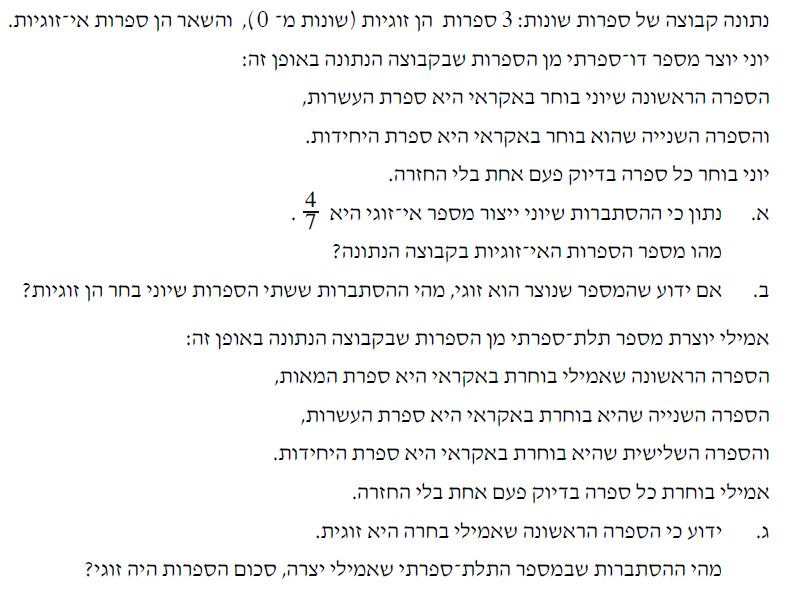
\includegraphics[width=.9\textwidth]{summer-2015a-3}
\end{center}

\textbf{סעיף א}

נסמן את קבוצת הספרות ב-%
$S$ \L{(sifarot)},
קבוצת הספרות הזוגיות ב-%
$Z$ \L{(zugi)},
קבוצת הספרות האי-זוגיות ב-%
$I$ \L{(i-zugi)}.
בחירה של ספרת העשרות ואחר כך ספרת היחידות מכוונת לעץ הסתברויות. במקום לרשום את מספרי הספרות בצמתים וההסתברויות על הקשתות, נפשט את התרשים ונרשום בכל צומת את ההסתברויות שליפת ספרה זוגית או אי-זוגית
$(P(Z=k_1),P(I=k_2))$.

\begin{center}
\begin{tikzpicture}
[grow=right,
level 1/.append style={text width=2cm,level distance=3.5cm,sibling distance=6em},
level 2/.append style={text width=2.5cm,level distance=4.5cm,sibling distance=3.5em}]
\node[text width=2cm] {$\left(\frac{3}{n},\frac{n-3}{n}\right)$} % root
child {
  node {$\left(\frac{3}{n-1},\frac{n-4}{n-1}\right)$}
    child {
      node {$\left(\frac{3}{n-2},\frac{n-5}{n-2}\right)\quad *$}
      edge from parent node[below,xshift=5mm,yshift=-1mm] {\R{אי-זוגי}}
    }
    child {
      node {$\left(\frac{2}{n-2},\frac{n-4}{n-2}\right)$}
      edge from parent node[above,xshift=5mm,yshift=1mm] {\R{זוגי}}
    }
    edge from parent node[below,yshift=-1mm] {\R{אי-זוגי}}
}
child { 
  node {$\left(\frac{2}{n-1},\frac{n-3}{n-1}\right)$}
    child {
      node {$\left(\frac{2}{n-2},\frac{n-4}{n-2}\right)\quad *$}
      edge from parent node[below,xshift=5mm,yshift=-1mm] {\R{אי-זוגי}}
    }
    child {
      node {$\left(\frac{1}{n-2},\frac{n-3}{n-2}\right)$}
      edge from parent node[above,xshift=5mm,yshift=1mm] {\R{זוגי}}
    }
    edge from parent node[above] {\R{זוגי}}
};
\end{tikzpicture}
\end{center}
המאורע
$YI$
שיוני ייצור מספר אי-זוגי יתרחש רק אם הבחירתו השנייה היא ספרה אי-זוגית. המסלולים המתאימים מסומנים בתרשים בכוכביות. נחשב את ההסתברות ונשווה להסתברות הנתונה:
\begin{eqn}
P(YI)&=&\frac{3}{n}\cdot\frac{n-3}{n-1} \;+\; \frac{n-3}{n}\cdot\frac{n-4}{n-1} = \frac{4}{7}\\
4n(n-1)&=&7(n-3)(n-1)\\
n&=&7\\
|I|&=&n-3=4\,.
\end{eqn}
נתון ש-%
$n\geq 3$
ולכן
$n\neq 1$
וניתן לצמצם את 
$n-1$.

\textbf{סעיף ב}

במספר זוגי הספרה האחרונה זוגית. נסמן ב-%
$Z2$
את המאורע ששתי הספרות זוגיות ונסמן ב-%
$ZA$ \L{aharona}
את המאורע ספרה אחרונה זוגית. הניסוח
"\textbf{אם ידוע}"
מכוון להסתברות מותנית:
\begin{eqn}
P(Z2/ZA) &=& \frac{P(Z2\:\cap\:ZA)}{P(ZA)}\\
&=&\frac{P(Z2)}{P(ZA)}\\
&=&\frac{\frac{3}{7}\cdot\frac{2}{6}}{1-\frac{4}{7}}=\frac{1}{3}\,.
\end{eqn}
השתמשנו ב-%
$Z2\subseteq ZA$ 
כי אם שתי הספרות זוגיות אזי הספרה האחרונה זוגית, ובעובדה ש-%
$P(ZA)=1-P(YI)$
שחישבנו בסעיף הקודם. החישוב של
$P(Z2)$
היא ההסתברות שמתקבלת מהמסלול העליון בעץ עבור בחירה של שתי ספרות זוגיות.

\textbf{סעיף ג}

הסכום יהיה זוגי רק אם שתי הספרות האחרונת הן זוגיות או אי-זוגיות:
\begin{eqn}
2k_1+2k_2+2k_3&=&2(k_1+k_2+k_3)\\
2k_1+2(k_2+1)+2(k_3+1)&=&2(k_1+k_2+k_3+1)\,.
\end{eqn}
נסמן ב-%
$Z1$
את המאורע שהספרה הראשונה זוגית ונסמן ב-%
$S$ \L{(sekhum)}
את המאורע שסכום הספרות זוגי. המילה "ידוע" מכוון להסתברות מותנית ולכן:
\begin{eqn}
P(S/Z1)&=& \frac{P(S\:\cap\:Z1)}{P(Z1)}\\
&=& \frac{P(S\:\cap\:Z1)}{P(Z1)}\\
&=&\frac{\frac{3}{7}\cdot\frac{2}{6}\cdot \frac{1}{5}+
\frac{3}{7}\cdot\frac{4}{6}\cdot \frac{3}{5}}
{\frac{3}{7}}=\frac{7}{15}\,.
\end{eqn}
המנה חושב משני המסלולים המסומנים בכוכביות בעץ ההסתברויות בעמוד הבא, כי הם מתחילים עם בחירה של ספרה זוגית ואז שני ואז או שתי ספרות זוגיות או שתי ספרות אי-זוגיות כדי לקבל סכום זוגי.
\begin{center}
\begin{tikzpicture}
[grow=right,
level 1/.append style={level distance=3cm,sibling distance=10em},
level 2/.append style={level distance=3cm,sibling distance=10em},
level 3/.append style={level distance=4cm,sibling distance=5em}]
\node {$\left(\frac{3}{7},\frac{4}{7}\right)$} % root
  child {
    node {$\cdots$}
    edge from parent node[below,yshift=-8pt] {\R{אי-זוגי}}
  }
child {
  node {$\left(\frac{2}{6},\frac{4}{6}\right)$}
child {
  node {$\left(\frac{2}{5},\frac{3}{5}\right)$}
    child {
      node {$\left(\frac{2}{4},\frac{2}{4}\right)\quad *$}
      edge from parent node[below,xshift=5mm,yshift=-2mm] {\R{אי-זוגי}}
    }
    child {
      node {$\left(\frac{1}{4},\frac{3}{4}\right)$}
      edge from parent node[above,xshift=5mm,yshift=2mm] {\R{זוגי}}
    }
    edge from parent node[below,yshift=-3mm] {\R{אי-זוגי}}
}
child { 
  node {$\left(\frac{1}{5},\frac{4}{5}\right)$}
    child {
      node {$\left(\frac{1}{4},\frac{3}{4}\right)$}
      edge from parent node[below,xshift=5mm,yshift=-2mm] {\R{אי-זוגי}}
    }
    child {
      node {$\left(\frac{0}{4},\frac{4}{4}\right)\quad *$}
      edge from parent node[above,xshift=5mm,yshift=2mm] {\R{זוגי}}
    }
    edge from parent node[above,yshift=2mm] {\R{זוגי}}
}
  edge from parent node [above,yshift=8pt] {\R{זוגי}}
};
\end{tikzpicture}
\end{center}

%%%%%%%%%%%%%%%%%%%%%%%%%%%%%%%%%%%%%%%%%%%%%%%%%%%%%%%%%

\newpage

\section{חורף תשע"ה}

\begin{center}
\selectlanguage{english}
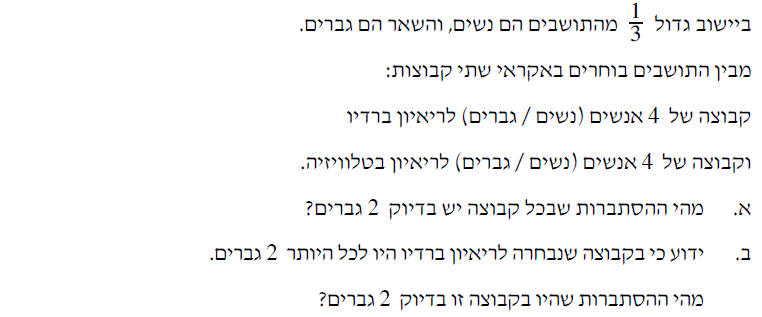
\includegraphics[width=.85\textwidth]{winter-2015-3}
\end{center}

המשמעות של "יישוב גדול" היא (כנראה) שאפשר לבחור את שתי הקבוצות בלי לשנות את ההסתברות של 
$\frac{1}{3}$
במהלך הבחירה, למרות שהבחירה היא ללא החזרה.

\textbf{סעיף א}

נסמן ב-%
$G2$
את המאורע של בחירת שני בגברים בקבוצה אחת ונסמן ב-%
$G22$
את המאורע של בחירת שני גברים בשתי הקבוצות. בחירת גבר נקראת הצלחה ולכן נשתמש בנוסחת ברנולי כדי לקבל את ההסתברות
\textbf{לבדיוק}
שתי הצלחות בקבוצה אחת:
\[
P(G2)={4 \choose 2}\left(\frac{2}{3}\right)^2\left(1-\frac{2}{3}\right)^2=\frac{8}{27}\,.
\]
לפי ההנחה שאין שינוי בהסתברות של הבחירה בין שתי הקבוצות, נקבל:
\[
P(G22)=P(G2)\cdot P(G2)=\frac{64}{729}\,.
\]

\textbf{סעיף ב}

נסמן את המאורע "לכל היותר שני גברים" ב-%
$G012$.
הניסוח
"\textbf{ידוע כי}"
מכוון להסתברות מותנית:
\begin{eqn}
P(G2/G012)&=&\frac{P(G2 \:\cap\: G012)}{P(G012)}\\
\end{eqn}
$G2\subseteq G012$
ולכן המנה היא
$G2=\frac{8}{27}$.
"לכל היותר שני גברים" הוא הסכום של שלוש נוסחאות ברנולי:
\[
\left(\frac{2}{3}\right)^0\left(\frac{1}{3}\right)^4 + {4\choose 1}\left(\frac{2}{3}\right)^1\left(\frac{1}{3}\right)^3 + {4\choose 2}\left(\frac{2}{3}\right)^2\left(\frac{1}{3}\right)^2=\frac{11}{27}\,
\]
והתשובה לשאלה היא:
\[
P(G2/G012)=\frac{\frac{8}{27}}{\frac{11}{27}}=\frac{8}{11}\,.
\]


% !TeX root = probability.tex

%%%%%%%%%%%%%%%%%%%%%%%%%%%%%%%%%%%%%%%%%%%%%%%%%%%%%%%%%%%%%

\section{קיץ תשע"ד מועד ב}

\begin{center}
\selectlanguage{english}
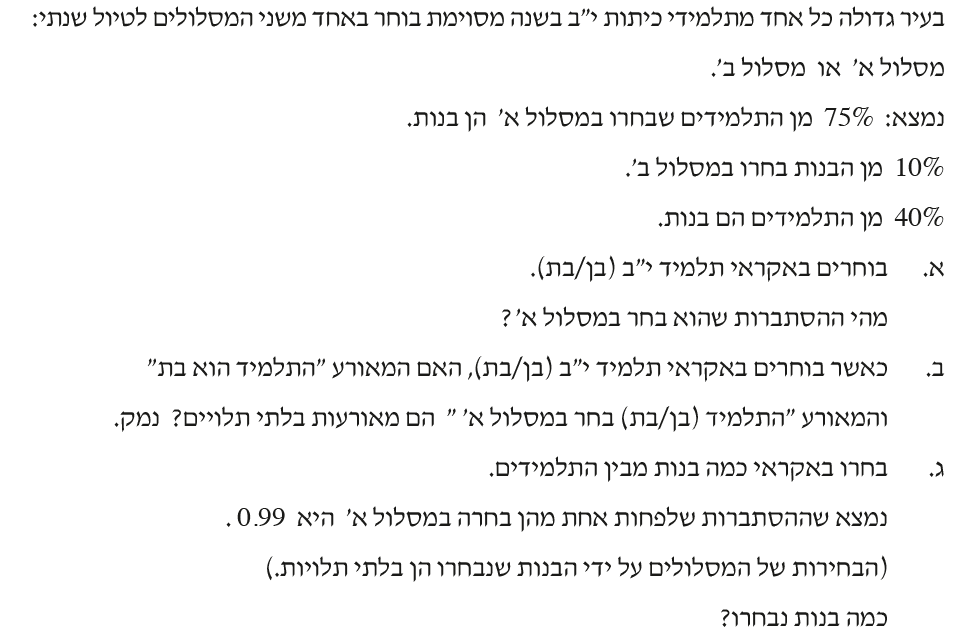
\includegraphics[width=.95\textwidth]{summer-2014b-3}
\end{center}

נמסן את הקבוצות בשאלה:
$G$ \L{(girl)}, $B$ \L{(boy)},
$MA$ \L{(maslul aleph)}, $MB$ \L{(maslul bet)}.
בגלל שיש שני זוגות של קבוצות נציג את ההסתברויות בטבלה. את הטבלה נמלא בשתי דרכים שונות, תחילה ישירות מהנתונים ואחר כך תוך שימוש בהסתברות מותנית.
\begin{center}
\selectlanguage{english}
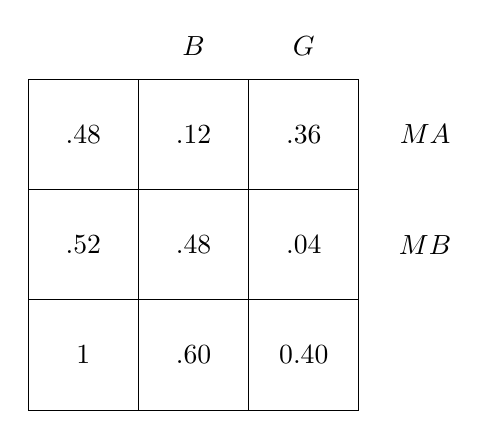
\begin{tikzpicture}[scale=1.4]
\draw (0,0) grid (3,3);
\node at (2.5,3.3) {$G$};
\node at (1.5,3.3) {$B$};
\node at (3.6,2.5) {$MA$};
\node at (3.6,1.5) {$MB$};
%\node at (2.5,2.7) {$.4-.04=$};
\node at (2.5,2.5) {$.36$};
%\node at (0.5,2.7) {$.36/.75=$};
\node at (0.5,2.5) {$.48$};
%\node at (1.5,2.7) {$.48-.36=$};
\node at (1.5,2.5) {$.12$};
%\node at (0.5,1.7) {$1-.48=$};
\node at (0.5,1.5) {$.52$};
\node at (0.5,0.5) {$1$};
%\node at (1.5,0.7) {$1-.4=$};
\node at (1.5,0.5) {$.60$};
%\node at (2.5,0.7) {\bfseries \R{נתון}};
\node at (2.5,0.5) {$0.40$};
%\node at (1.5,1.7) {$.52-.04=$};
\node at (1.5,1.5) {$.48$};
%\node at (2.5,1.7) {$.1\times .4=$};
\node at (2.5,1.5) {$.04$};
\end{tikzpicture}
\end{center}

\textbf{דרך א'}

נתון ש-% 
$P(G)=0.40$
ונתון ש-%
$10\%$
מהם בחרו במסלול ב', ולכן 
$P(G\cap MB)= .04$,
ומהסתברות משלימה
$P(G\cap MA)= .36$.
הנתון האחרון הוא ש-%
$0.75 P(MA) = 0.36$
ולכן 
$P(MA)=0.36/0.75=0.48$.
את שאר התאים ניתן למלא מהסתברויות משלימות.

\textbf{דרך ב'}

שוב נמלא את התא הימני למטה ב-%
$P(G)=0.40$.
נמשיך:
\begin{eqnarray*}
P(MB/G) &=& \frac{P(MB \:\cap\: G)}{P(G)}=0.10\\
P(MB \:\cap\: G) &=& P(G)P(MB/G) = 0.40\cdot 0.10 = 0.04\,.
\end{eqnarray*}
עוד הסתברות מותנית:
\begin{eqnarray*}
P(G/MA) &=& \frac{P(G \:\cap\: MA)}{P(MA)}=0.75\\
P(MA) &=& \frac{P(G \:\cap\: MA)}{P(G/MA)}=\frac{0.36}{0.75}=0.48\,,
\end{eqnarray*}
ונמלא את שאר התאים באמצעות הסתברויות משלימות.

\textbf{סעיף א}

$P(MA)=0.48$.

\textbf{סעיף ב}
\begin{eqnarray*}
P(G\cap MA) &=&0.36\\
P(G)P(MA)&=&0.40\cdot 0.48=0.19\,.
\end{eqnarray*}
$0.36\neq 0.19$
ולכן המאורעות אינם בלתי תלויים.

\textbf{סעיף ג}

ניתן לחשב "לפחות אחת" על ידי חישוב הסתברות של "אף אחת". ההסתברות שבת לא תבחר מסלול א' היא ההסתברות שהיא תבחר מסלול ב':
\begin{eqnarray*}
P(MB/G) &=& \frac{P(MB \:\cap\: G}{P(G)}= \frac{0.04}{0.40}=0.10\\
(0.10)^n&=&1-0.99=0.01\\
n&=&2\,.
\end{eqnarray*}

%%%%%%%%%%%%%%%%%%%%%%%%%%%%%%%%%%%%%%%%%%%%%%%%%%%%%%%%%%%%%%%%%%%

\section{קיץ תשע"ד מועד א}

\begin{center}
\selectlanguage{english}
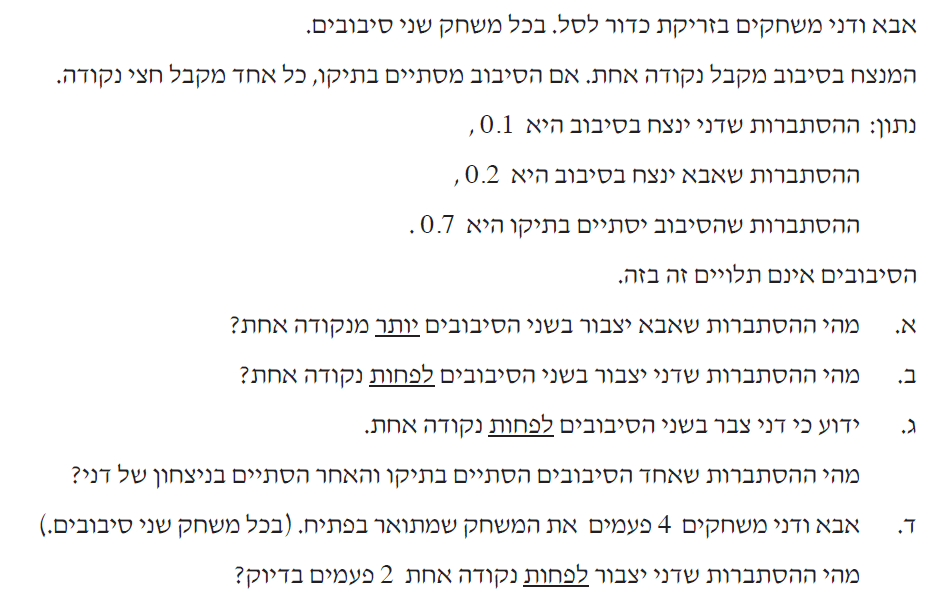
\includegraphics[width=.9\textwidth]{summer-2014a-3}
\end{center}

נסמן ב-%
$D1, D2$ \L{(dani)}
את המאורע שדני מנצח בסיבוב אחד או שניים, נסמן ב-%
$A1, A2$ \L{(abba)}
את המאורע שאבא מנצח בסיבוב אחד או שניים, ונסמן ב-%
$T1, T2$ \L{(teku)}
את המאורע שיהיה תיקו בסיבוב אחד או שניים. השאלה שואלת על סדרה של שני סבבים וזה מכוון לעץ הסתברויות (בעמוד הבא). בסוף כל מסלול רשום מספר הנקודות שאבא צבר ומספר הנקודות שדני צבר.

\begin{figure}
\begin{center}
\selectlanguage{english}
\begin{tikzpicture}
[align=left,grow=right,
level 1/.append style={level distance=3cm,sibling distance=9em},
level 2/.append style={level distance=4cm,
                       sibling distance=3.5em}]
\node[left] {$0$} % root
child {
  node[right] {$\frac{1}{2}$}
    child {
      node[below right,xshift=10pt,yshift=4pt] {$(i) A2=1,D2=1$}
      edge from parent node[below,yshift=-1mm] {$0.7$}
    }
    child {
      node[right,xshift=10pt] 
        {$(h) A2=\frac{1}{2},D2=\frac{1}{2}$}
      edge from parent node[below,xshift=4mm] {$0.1$}
    }
    child {
      node[right,xshift=10pt] 
        {$(g) A2=1\frac{1}{2},D2=\frac{1}{2}$}
      edge from parent node[above,yshift=1mm] {$0.2$}
    }
    edge from parent 
      node[below,xshift=-4mm,yshift=-3mm] {\R{תיקו} $0.7$}
}
child {
  node[right] {$0$}
    child {
      node[right,xshift=10pt] 
        {$(f) A2=\frac{1}{2},D2=1\frac{1}{2}$}
      edge from parent node[below,yshift=-1mm] {$0.7$}
    }
    child {
      node[right,xshift=10pt] {$(e) A2=0,D2=2$}
      edge from parent node[below,xshift=4mm] {$0.1$}
    }
    child {
      node[right,xshift=10pt] {$(d) A2=1,D2=1$}
      edge from parent node[above,yshift=1mm] {$0.2$}
    }
    edge from parent 
      node[below] {\R{דני} $0.1$}
}
child {
  node[right] {$1$}
    child {
      node[right,xshift=10pt] {$(c) A2=1\frac{1}{2},D2=\frac{1}{2}$}
      edge from parent node[below,yshift=-1mm] {$0.7$}
    }
    child {
      node[right,xshift=10pt] {$(b) A2=1,D2=1$}
      edge from parent node[below,xshift=4mm] {$0.1$}
    }
    child {
      node[above right,xshift=10pt] {$(a) A2=2, D2=0$}
      edge from parent node[above,yshift=1mm] {$0.2$}
    }
    edge from parent
       node[above,xshift=-4mm,yshift=3mm] {\R{אבא} $0.2$}
};
\end{tikzpicture}
\end{center}
\end{figure}

\textbf{סעיף א}

במסלול בהם אבא צובר יותר מנקודה אחת הם
\L{(a), (c), (g)},
וההסתברות היא:
\[
P(A2>1)=0.2\cdot 0.2 \,+\, 0.2\cdot 0.7 \,+\, 0.7\cdot 0.2 \,=\,0.32\,.
\]


\textbf{סעיף ב}

המסלולים בהם דני צבר לפחות נקודה אחת הם
\L{(b), (d), (e), (f), (h), (i)}
וההסתברות היא:
\[
P(D2\geq 1)=0.2\cdot 0.1 \,+\,0.1\cdot 0.2 \,+\, 0.1\cdot 0.1 \,+\,0.1\cdot 0.7 \,+\, 0.7\cdot 0.1\,+\,0.7\cdot 0.7\,=\,0.68\,.
\]


\textbf{סעיף ג}

הניסוח "ידוע" מכוון להסתברות מותנית, אבל
$D1\cup T1\subseteq D2\geq 1$
ולכן:
\begin{eqnarray*}
P((D1\cup T1)/D2\geq 1)&=&\frac{P((D1\cup T1) \:\cap\: D2\geq 1)}
  {D2\geq 1}\\
  &=&\frac{P(D1\cup T1)}{D2\geq 1}\\
\frac{0.1\cdot 0.7 \,+\, 0.7\cdot 0.1}{0.68} &=& \frac{7}{34}= 0.2059\,,  
\end{eqnarray*}
כי המסלולים המתאימים הם 
\L{(f), (h)}.

\textbf{סעיף ד}

נשמתמש בנוסחת ברנולי כי למצוא את ההסתברות לבדיוק פעמיים:
\[
{4\choose 2}P(D2)^2\: (1-P(D2)^2 =
{4\choose 2} (0.32)^2 (0.68)^2= 0.2841\,.
\]

%%%%%%%%%%%%%%%%%%%%%%%%%%%%%%%%%%%%%%%%%%%%%%%%%%%%%%%%

\section{חורף תשע"ד}

\begin{center}
\selectlanguage{english}
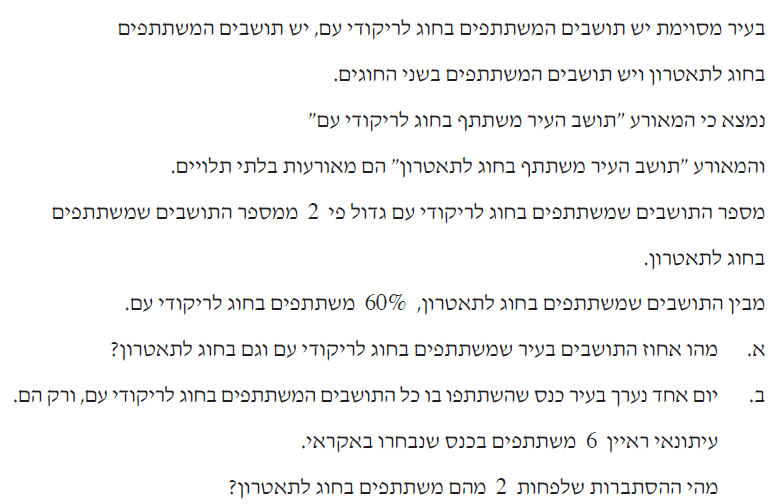
\includegraphics[width=.9\textwidth]{winter-2014-3}
\end{center}

נסמן ב-%
$T$ \L{(theatron)}
את המשתתפים בתאטרון ונסמן ב-%
$R$ \L{(rikudei)}
את המשתתפים בריקודי עם. המילה "מבין" מכוונת להתסברות מותנית. ההסתברויות הן של זוגות של מאורעות ולכן נשתמש בטבלה.


נתון
$P(R/T)=0.6$
ושהאירועים בלתי תלויים. נחשב:
\[
P(R/T)=\frac{P(R\cap T)}{P(T)}=\frac{P(R)\cdot P(T)}{P(T)}=P(R)=0.06\,.
\]
ביחד עם הנתון
$P(R)=2P(T)$
נתחיל למלא את הטבלה:
\begin{center}
\selectlanguage{english}
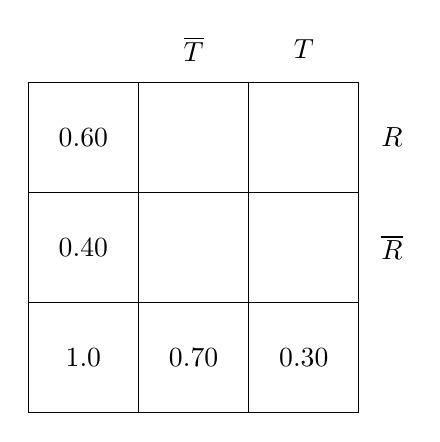
\begin{tikzpicture}[scale=1.4]
\draw (0,0) grid (3,3);
\node at (2.5,3.3) {$T$};
\node at (1.5,3.3) {$\overline{T}$};
\node at (3.3,2.5) {$R$};
\node at (3.3,1.5) {$\overline{R}$};
\node at (0.5,2.5) {$0.60$};
\node at (2.5,0.5) {$0.30$};
\node at (.5,.5) {$1.0$};
\node at (1.5,.5) {$0.70$};
\node at (.5,1.5) {$0.40$};
\end{tikzpicture}
\end{center}
שוב נסתמך על העובדה שהאירועים בלתי תלויים ונקבל:
\[
P(R\cap T)=P(R)\cdot P(T)=0.60\cdot 0.30=0.18\,,
\]
וניתן למלא את הטבלה לפי הסתברויות משלימות:
\begin{center}
\selectlanguage{english}
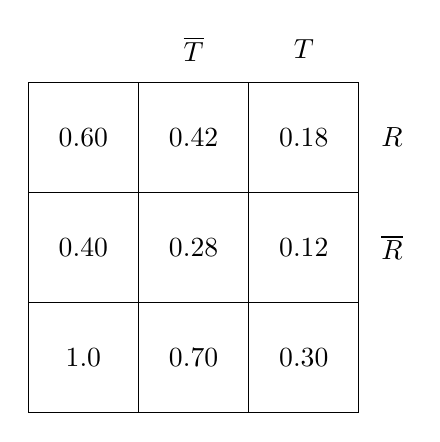
\begin{tikzpicture}[scale=1.4]
\draw (0,0) grid (3,3);
\node at (2.5,3.3) {$T$};
\node at (1.5,3.3) {$\overline{T}$};
\node at (3.3,2.5) {$R$};
\node at (3.3,1.5) {$\overline{R}$};
\node at (2.5,2.5) {$0.18$};
\node at (0.5,2.5) {$0.60$};
\node at (1.5,2.5) {$0.42$};
\node at (0.5,1.5) {$0.40$};
\node at (0.5,0.5) {$1.0$};
\node at (1.5,0.5) {$0.70$};
\node at (2.5,0.5) {$0.30$};
\node at (1.5,1.5) {$0.28$};
\node at (2.5,1.5) {$0.12$};
\end{tikzpicture}
\end{center}

\textbf{סעיף א}

$P(R\cap T)=0.18$.

\textbf{סעיף ב}

הניסוח "כל התושבים המשתתפים בחוג לריקודי עם, ורק הם" מכוונות להסתברות מותנית:
\[
P(T/R) = \frac{P(T\cap R)}{P(R)} = \frac{P(T)P(R)}{P(R)}= P(T)=0.30\,.
\]
כדי לחשב "לפחות שניים" נשתמש בנוסחת ברנולי ונחשב את המשלים ל-"אפס או אחד":
\[
P(T\geq 2/R)=1-{6\choose 0}(0.3)^0(0.7)^6 -{6\choose 1}(0.3)^1(0.7)^5=0.5798\,.
\]

% !TeX root = probability.tex

%%%%%%%%%%%%%%%%%%%%%%%%%%%%%%%%%%%%%%%%%%%%%%%%%%%%%%%%

\section*{המלצות}

\addcontentsline{toc}{section}{\large המלצות}

\begin{itemize}
\item
קרא בזהירות את השאלות. לעתים הן ארוכות וחשוב להבין את המשמעות של כל פסקה.

\item
כמעט כל הבחינות מכילות שאלות על הסתברות מותנית. ניסוחים רבים מכוונים להסתברות מותנית וחשוב להכיר אותם!

\begin{itemize}
\item
הניסוח השכיח ביותר משתמש במילים
"\textbf{אם ידוע ש-}"
או
"\textbf{ידוע כי}".

\item
בבחינה של חורף תשע"ז כתוב "%
\textbf{אם} $\ldots$ ,
\textbf{מהי ההסתברות} $\ldots$".
לא לגמרי ברור שלמילה "אם" יש משמעות של "אם ידוע", אבל זאת הכוונה.

\item
לעתים קרובות )בחינה של קיץ תשע"ה ב'( כתוב "%
\textbf{מה ההסתברות לבחור} $\ldots$
\textbf{מבין} $\ldots$".

\item
יוצא מן הכלל: בבחינה של קיץ תשע"ו א' כתוב
"\textbf{מבין}
כל הנבחנים". המילה "מבין" בדרך כלל מכוונת להסתברות מותנית, אבל כאשר "מבין" מתייחס ל-%
"\textbf{כל}
הנבחנים", אין הסתברות מותנית. לחילופין אפשר לחשב הסתברות מותנית כאשר החיתוך מצטמצם:
\[
P(X/\textrm{\R{כל הנבחנים}})=
\frac{P(X\cap \textrm{\R{כל הנבחנים}})}
{P(\textrm{\R{כל הנבחנים}})} = 
\frac{P(X)}{1}=P(X)\,.
\]

\item
בבחינה של קיץ תשע"ח א' הניסוח הוא: "%
$n\%$
נעזרו בחבריהם 
$N$
ו-%
$\displaystyle\frac{k}{n}$
\textbf{מהם}
עברו את הבחינה
$A$".
ברור ש-%
$P(A\cap N) = k$,
אבל נבדוק לפי הנוסחה להסתברות מונתית:
\begin{eqnarray*}
P(A/N) &=& \frac{P(A\cap N)}{P(N)} = \frac{k}{n}\\
P(A\cap N)&=&k\,.
\end{eqnarray*}

\item
בבחינה של חורף תשע"ד יש ניסוח אחר: "כל התושבים המשתתפים ב-
$\ldots$,
\textbf{ורק הם}".
\end{itemize}

%%%%%%%%%%%%%%%%%%%%%%%%%%%%%%%%%%%%

\item
כאשר יש חיתוך בחישוב של הסתברות מותנית, לעתים קרובות ניתן לפשט את החישוב. בבחינה של קיץ תשע"ז א' יש לחשב
$P(D=4\cap D\ge 3)$,
אבל אם ערך גדול או שווה
$3$
\textbf{וגם}
שווה ל-%
$4$,
אז הוא שווה ל-%
$4$, 
ולכן מספיק לחשב
$P(D=4)$.

%%%%%%%%%%%%%%%%%%%%%%%%%%%%%%%%%%%%

\item
אם שני אירועים בלתי תלויים, חישוב ההסתברות המותנית מצטמצם:
\[
P(A/B) = \frac{P(A\cap B)}{P(B)} = \frac{P(B)\cdot P(A)}{P(A)}= P(B)\,.
\]
מצב זמ מופיע בבחינות של חורף תשע"ז, חורף משע"ח, קיץ תשע"ה א', חורף תשע"ד.
%%%%%%%%%%%%%%%%%%%%%%%%%%%%%%%%%%%%



\item
המילה 
\textbf{בדיוק}
מכוונת לחישוב אחד של נוסחת ברנולי, כי נתון כמה "הצלחות" צריכות להיות וגם כמה "כשלונות".

%%%%%%%%%%%%%%%%%%%%%%%%%%%%%%%%%%%%

\item
בבחינה של קיץ תשע"ז א' כתוב "%
\textbf{בוחרים באקראי}
$\ldots$,
\textbf{עד של-}
$3$
מהם
\textbf{בדיוק}
יש קלנועית". המשמעות של "עד ש-" היא שמפסיקים את הבחירה האקראית כאשר הבחירה 
\textbf{האחרונה} 
היא "הצלחה". במקרה זה נשארו שתי "הצלחות" שיש לחשב את ההסתברות שלהן לפי נוסחת ברנולי, ואז להכפיל בהסתברות של "הצלחה" בבחירה האחרונה:
\[
\overbrace{\pm\;\pm\;\pm\;\pm\;\pm}^{2/5}\quad\quad \overbrace{+}^{1/1}\,.
\]

%%%%%%%%%%%%%%%%%%%%%%%%%%%%%%%%%%%%

\item
בבחינה של קיץ תשע"ז ב' הביטוי "מוציאים באקראי
$\ldots$",
ובהמשך הביטוי "מוציאים באקראי
\textbf{שוב}
$\ldots$"
מכוון לשימוש בעץ כדי לתאר את הבחירה הסדרתית.

%%%%%%%%%%%%%%%%%%%%%%%%%%%%%%%%%%%%

\item
בבחינה של קיץ תשע"ח א' המשמעות של הניסוח "%
\textbf{לפחות אחת}
משתי הטענות I, II היא שהאירוע קורה אם קורה אחד מהאירועים I, II,
\textbf{או שניהם},
המסומן I
$\cup$
II".
יש שתי דרכים לחשב את ההסתברות:
\begin{eqnarray*}
P(\textrm{I} \cup \textrm{II}) &=& P(\textrm{I}) + P(\textrm{II}) - P(\textrm{I} \cap \textrm{II})\\
P(\textrm{I} \cup \textrm{II}) &=& P(\textrm{I}-\textrm{II}) + P(\textrm{II}-\textrm{I}) + P(\textrm{I} \cap \textrm{II})\,.
\end{eqnarray*}

%%%%%%%%%%%%%%%%%%%%%%%%%%%%%%%%%%%%

\item
בבחינה של  קיץ תשע"ח ב' יש לחשב את ההסבתרות לפי נוסחת ברנולי
${n \choose k}p^k(1-p)^{n-k}$.
\begin{itemize}
\item
אם
$k=0$
אזי
${n\choose 0}=1$
והנוסחה מצטמצמת ל-%
$p^0(1-p)^{n-0}=(1-p)^n$.
\item 
אם
$k=n$
אזי
${n\choose n}=1$
והנוסחה מצטמצמת ל-%
$p^n(1-p)^{n-n}=p^n$.
\end{itemize}


%%%%%%%%%%%%%%%%%%%%%%%%%%%%%%%%%%%%

\item
בבחינות של קיץ תשע"ו א' ו-ב' יש שלוש תוצאות לפעולה במקום שתיים. סכום ההסתברויות חייב להיות אחד, ולכן כאשר מחשבים משלים להסתברות אחת, יש להחסיר את שתי ההסתברויות האחרות. בבחינה של מועד ב' ההסתברות לתיקו היא אחד פחות ההסתברות שיעל תנצח פחות ההסתברות אנה תנצח:
\[
P(\textrm{\R{תיקו}}) =
1 - (P(\textrm{\R{יעל}})+
P(\textrm{\R{אנה}})) = 
1 - P(\textrm{\R{יעל}})-
P(\textrm{\R{אנה}}) \,.
\]

\item 
במספר בחינות (חורף תשע"ה, קיץ תשע"ד ב', קיץ תשע"ה ב') מתואר מצב הנקרא "שליפה ללא החזרה". אם יש מספר נמוך של תושבים, השליפות לא בלתי-תלויות. כאשר כתוב "ישוב גדול", "עיר גדולה", "אוניברסיטה גדולה", אני מניח שכוונה שיש מספר כל כך גדול של תושבים שאין שינוי משמעותי בהסתברות משליפה אחת לבאה אחריה.
\end{itemize}


\end{document}


\tikzsetfigurename{geometry}
% !TeX root = bagrut-all.tex

\selectlanguage{hebrew}

\chapter{גיאומטריה}

\section{קיץ תשע"ח מועד ב}

\begin{center}
\selectlanguage{english}
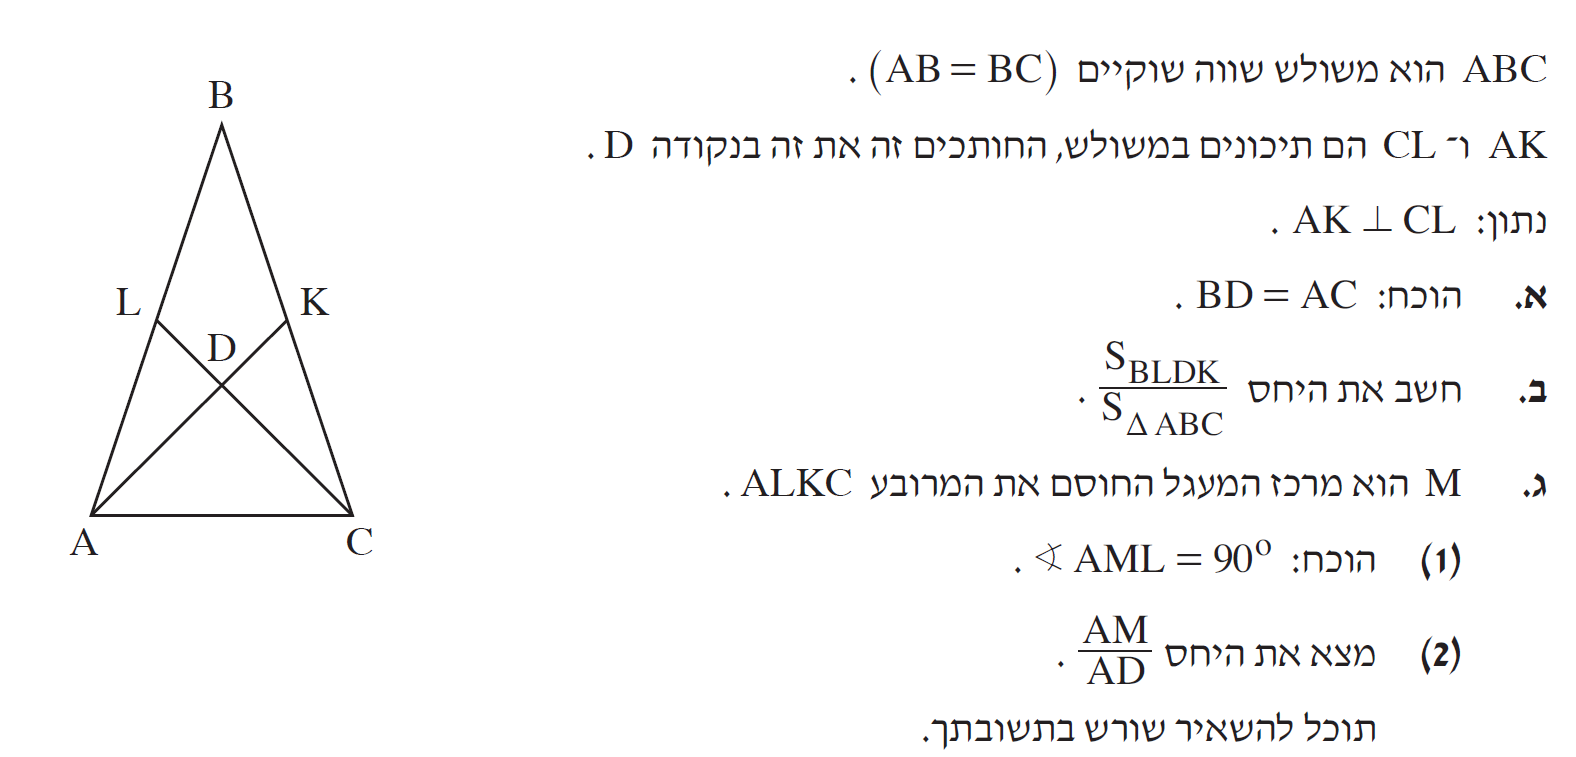
\includegraphics[width=\textwidth]{summer-2018b-4}
\end{center}

\vspace{-3ex}

\textbf{סעיף א}

כאשר יש תיכונים נחתכים מיד חושבים על משפט
$45$
"שלושת התיכונים במשולש נחתכים בנקודה אחת", ובמשפט
$46$
"נקודת חיתוך התיכונים מחלקת כל תיכון ביחס
$2:1$".
נבנה
$BE$,
התיכון מ-%
$B$
ל-%
$AC$,
שחותך את מפגש התיכונים האחרים ב-%
$D$.
$BE\perp AC$
לפי משפט
$6$
"במשולש שווה-שוקיים , חוצה זווית הראש, התיכון לבסיס והגובה לבסיס מתלכדים". קל להראות שהתיכונים
$AK,CL$
שווים, כי 
$\triangle AED\cong \triangle CED$
ואז
$\triangle LDA\cong \triangle KDC$.
סימנו את הקטעים
$DK=DL=a$,
$DC=DA=2a$.
\begin{center}
\selectlanguage{english}
\begin{tikzpicture}[scale=.7]
\draw[thick] (0,0) coordinate (A) -- (6,0) coordinate (C);
\draw[thick] (A) -- (3,8) coordinate (B) -- (C);
\coordinate (K) at ($(B) ! .5 ! (C)$);
\coordinate (L) at ($(A) ! .5 ! (B)$);
\draw[thick,name path=ak] (A) -- (K);
\draw[thick,name path=cl] (C) -- (L);
\path[name intersections={of=ak and cl,by={D}}];
\fill (A) node[below] {$A$} circle(1.5pt);
\fill (B) node[above] {$B$} circle(1.5pt);
\fill (C) node[below] {$C$} circle(1.5pt);
\fill (D) node[above right,xshift=-2pt,yshift=8pt] {$D$} circle(1.5pt);
\fill (K) node[right] {$K$} circle(1.5pt);
\fill (L) node[left] {$L$} circle(1.5pt);
\draw[rotate=-45] (D) rectangle +(7pt,7pt);
\draw[dashed,thick] (B) |- (A);
\coordinate (E) at ($(A)!.5!(C)$);
\fill (E) node[below] {$E$} circle(1.5pt);
\draw (E) rectangle +(7pt,7pt);
\path (A) -- node[right,yshift=-4pt] {$2a$} (D) -- node[right,yshift=-4pt] {$a$} (K);
\path (C) -- node[left,yshift=-4pt] {$2a$} (D) -- node[left,yshift=-4pt] {$a$} (L);
\path (B) -- node[left] {$2b$} (D) -- node[left] {$b$} (E);
\path (A) -- node[below] {$b?$} (E);
\path (E) -- node[below] {$b?$} (C);
\end{tikzpicture}
\end{center}

\np

אם נוכיח ש-%
$AE=EC=DE$,
נקבל ש-% 
$BD=2b=2DE=AE+ED=AC$.
לפי משפט
$6$,
$BE$
הוא חוצה זווית של
$\angle ABC$,
וגם של
$\angle ADC$
כי חוצה הזווית והתיכון מתלכדים. נתון ש-%
$AK\perp CL$
כך ש-%
$\angle ADC=90^\circ$,
ולכן 
$\angle ADE,\angle CDE$
שוות ל-%
$\frac{1}{2}\cdot 90^\circ=45^\circ$.
במשולשים ישר-זווית
$\triangle ADE,\triangle CDE$,
זוויות חדות של
$45^\circ$,
ולכן גם הזוויות
$\angle DAE,\angle DCE$
שוות
$45^\circ$,
והמשולשים שווה-שוקיים. מכאן ש-%
$AE=EC=DE=b$.

אפשרות אחרת, פשוטה יותר, להוכיח
$AE=EC=DE=b$
היא להשתמש במשפט
$86$
"במשולש ישר-זווית התיכון ליתר שווה למחצית היתר" ב-%
$\triangle ADC$.


\textbf{סעיף ב}

כדאי לחשב 
$S_{BLDK}$
על ידי חיסור שטח המצולע
$ALDKC$
מהשטח של
$\triangle ABC$,
כי המצולע מורכב ממשולשים ישר-זווית וחישוב השטח שלהם קל מאוד:
\erh{12pt}
\begin{equationarray*}{rcl}
S_{ALDKC}&=&S_{ADL}+S_{KDC}+S_{ADC}=2S_{ADL}+S_{ADC}\\
&=&2\cdot \frac{1}{2} AD\cdot DL + \frac{1}{2} AC\cdot DE\\
&=&2a\cdot a + \frac{1}{2}\cdot 2b \cdot b\\
&=&2a^2+b^2\,.
\end{equationarray*}
אפשר להניח שהיחס המבוקש אינו תלוי באורכן של הצלעות, לכן נחפש דרך להביע את שטח המצולע
$S_{ALDKC}$
כפונקציה של
$b$
בלבד. ממשפט פיתגורס על
$\triangle ADE$:
\erh{12pt}
\begin{equationarray*}{rcl}
b^2+b^2&=&(2a)^2=4a^2\\
%b^2&=&2a^2\\
S_{ALDKC}&=&2a^2+b^2=2\cdot\frac{1}{4}(b^2+b^2)+ b^2=2b^2\\
S_{ABC}&=&\frac{1}{2}AC\cdot BE= \frac{1}{2}2b\cdot 3b=3b^2\\
S_{BLDK}&=&S_{ABC}-S_{ALDKC}=3b^2-2b^2=b^2\\
\frac{S_{BLDK}}{S_{ABC}}&=&\frac{b^2}{3b^2}=\frac{1}{3}\,.
\end{equationarray*}

\np

\textbf{סעיף ג}
$(1)$

לא התקדמתי עד שציירתי תרשים חדש עם המעגל וראיתי שהזווית ההיקפית
$\angle LKA$
נשענת על המיתר עליו נשענת הזווית המרכזית
$\angle AML$,
כך ש-%
$\angle AML=2\angle LKA$
לפי משפט
$69$
"במעגל, זווית היקפית שווה למחצית הזווית המרכזית הנשענת על אותה הקשת". אבל לפי משפט
$14$
"קטע אמצעים במשולש מקביל לצלע השלישית ושווה למחציתה",
$LK\|AC$,
ולכן
$\angle KAC=\angle LKA=\alpha$
לפי זוויות מתחלפות, והוכחנו בסעיף הקודם ש-%
$\alpha = 45^\circ$,
לכן,
$\angle AML = 2\alpha=90^\circ$.

\begin{center}
\selectlanguage{english}
\begin{tikzpicture}
\clip (-1,-2.2) rectangle +(8,7);
\draw[thick] (0,0) coordinate (A) -- (6,0) coordinate (C);
\path (A) -- (3,8) coordinate (B) -- (C);
\coordinate (K) at ($(B) ! .5 ! (C)$);
\coordinate (L) at ($(A) ! .5 ! (B)$);
\path[name path=ak] (A) -- (K);
\draw[thick,name path=cl] (C) -- (L);
\path[name intersections={of=ak and cl,by={D}}];
\fill (A) node[below,xshift=-4pt] {$A$} circle(1.5pt);
\fill (C) node[below,xshift=4pt] {$C$} circle(1.5pt);
\fill (D) node[above] {$D$} circle(1.5pt);
\fill (K) node[right,xshift=4pt] {$K$} circle(1.5pt);
\fill (L) node[left,xshift=-4pt] {$L$} circle(1.5pt);
\draw[rotate=135] (D) rectangle +(7pt,7pt);
\tkzCircumCenter(A,L,K)\tkzGetPoint{M}
\tkzDrawCircle[thick,name path=circle](M,A)
\fill (M) node[above right] {$M$} circle(1.5pt);
\draw[rotate=110] (M) rectangle +(7pt,7pt);
\draw[thick] (A) -- (M);
\draw[thick,name path=ml] (M) -- (L);
\path[name intersections={of=ak and ml,by={G}}];
\fill (G) node[left,xshift=-4pt] {$G$} circle(1.5pt);
\draw[thick] (A) -- (L) -- (K) -- (C);
\draw[thick] (A) -- (K);
\node[below left,xshift=-8pt] at (K) {$\alpha$};
\node[left,xshift=-6pt,yshift=4pt] at (M) {$2\alpha$};
\draw[thick] ($(A)+(10mm,0)$) arc[start angle=0,end angle=45,radius=9mm];
\node[above right,yshift=10pt,xshift=22pt] at (A) {$\alpha$};
\path (L) -- node[right] {$a$} (D);
\path (A) -- node[left,xshift=4pt,yshift=8pt] {$2a$} (D);
\end{tikzpicture}
\end{center}

\textbf{סעיף ג}
$(2)$

תחילה שמתי לב ש-%
$\triangle MGA\sim \triangle DGL$
כי במשלושים ישר-זווית, הזוויות
$\angle MGA=\angle DGL$
קודקודיות. גישה זו לא הצליחה כי לא מצאתי דרך לבטא את הקשר בין
$AD$
לבין 
$AG, GD$.
לבסוף שמתי לב שלמשולשים
$\triangle LDA,\triangle LMA$
יתר משותף, והמשולש
$\triangle LMA$
שווה-שוקיים כי שתי הצלעות
$AM,ML$
הן רדיוסים. ממשפט פיתגורס:
\erh{12pt}
\begin{equationarray*}{rcl}
AM^2+ML^2&=&AL^2\\
%AM&=&ML\\
2AM^2&=&AL^2\\
LD^2+AD^2&=&AL^2\\
%LD^2&=&a^2\\
a^2+AD^2&=&2AM^2\\
%AD^2&=&4a^2\\
\frac{1}{4}AD^2+AD^2&=&2AM^2\\
\frac{AM}{AD}&=&\sqrt{\frac{5}{8}}\,.
\end{equationarray*}

%%%%%%%%%%%%%%%%%%%%%%%%%%%%%%%%%%%%%%%%%%%%%%%%%%%%%%%%%%%%%%%%%%%

\np

\section{קיץ תשע"ח מועד א}

\begin{center}
\selectlanguage{english}
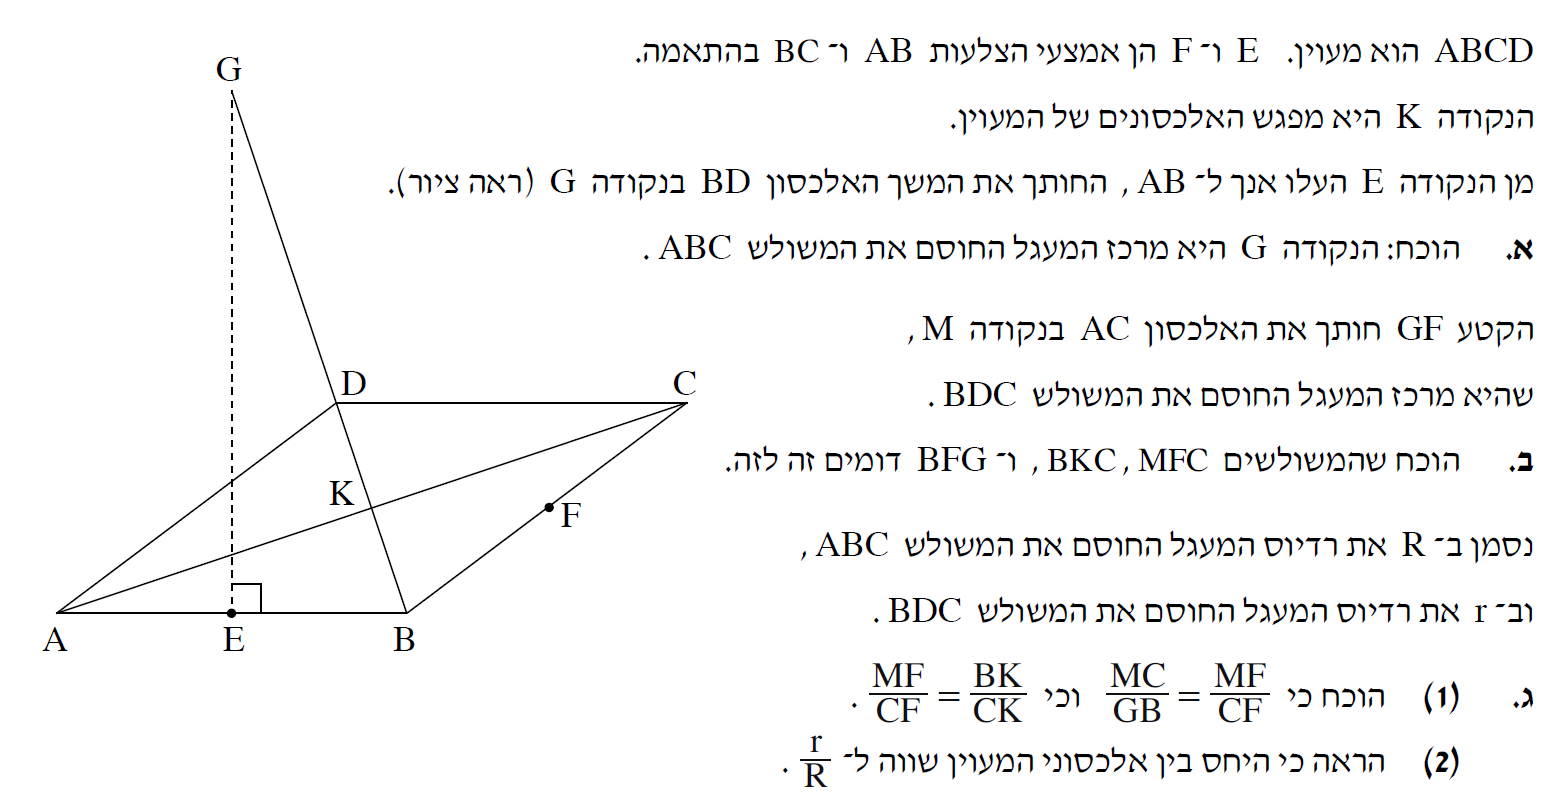
\includegraphics[width=\textwidth]{summer-2018a-4}
\end{center}

\vspace{-2ex}

\textbf{סעיף א}

כדי להוכיח ש-%
$G$
היא מרכז של מעגל חוסם נשתמש במשפט
$54$
"במשולש, שלושת האנכים האמצעיים נחתכים בנקודה אחת , שהיא מרכז המעגל החוסם את המשולש". צריך להוכיח ש-%
$GE,GB$
הם אנכים אמצעיים של
$\triangle ABC$.
מעוין הוא מקבילית עם צלעות שוות, וכמקבילית, ניתן להשתמש במשפט 
$28$
"במקבילית האלכסונים חוצים זה את זה". סימנו בציר את אורכי האלכסון
$AC$
ב-%
$b$.
ביחד עם משפט
$35$
"במעוין האלכסונים מאונכים זה לזה", 
$GB$
הוא אנך אמצעי ל-%
$AC$.
נתון שנקודת
$E$
היא אמצע של 
$AB$,
וש-%
$GE$
הוא אנך ל-%
%
$AB$,
ולכן
$G$
היא נקודת החיתוך של שני אנכים אמצעיים ומכאן מרכז המעגל החוסם את
$\triangle ABC$.

\begin{center}
\selectlanguage{english}
\begin{tikzpicture}[scale=.8]
\draw[thick] (0,0) coordinate (A) -- ++(40:5) coordinate (D) -- ++(5,0) coordinate (C);
\draw[thick] (A) -- ++(5,0) coordinate (B) -- (C);
\coordinate (F) at ($(B) ! .5 ! (C)$);
\coordinate (E) at ($(A) ! .5 ! (B)$);
\fill (A) node[below] {$A$} circle(1.5pt);
\fill (B) node[below] {$B$} circle(1.5pt);
\fill (C) node[above] {$C$} circle(1.5pt);
\fill (D) node[above right] {$D$} circle(1.5pt);
\fill (E) node[below] {$E$} circle(1.5pt);
\fill (F) node[right,xshift=2pt] {$F$} circle(1.5pt);
\draw[thick,name path=ac] (A) -- (C);
\path[name path=bg] (B) -- ($(B) ! 2.3 ! (D)$);
\path[name path=ge] (E) -- +(0,7.3);
\path[name intersections={of=ge and bg,by={G}}];
\fill (G) node[above] {$G$} circle(1.5pt);
\draw[dashed,thick] (G) -- (E);
\draw[thick] (G) -- (B);
\path[name intersections={of=ac and bg,by={K}}];
\fill (K) node[above,xshift=5pt,yshift=2pt] {$K$} circle(1.5pt);
\draw[rotate=110] (K) rectangle +(7pt,7pt);
\draw (E) rectangle +(7pt,7pt);
\path (A) -- node[below] {$a$} (E) -- node[below] {$a$} (B);
\path (B) -- node[right,xshift=2pt] {$a$} (F) -- node[right,xshift=2pt] {$a$} (C);
\path (A) -- node[below,near end] {$b$} (K) -- node[below,near start] {$b$} (C);
\end{tikzpicture}
\end{center}

\np

\textbf{סעיף ב}

ההוכחה שהמשולשים דומים תהיה קל יותר אם נבנה מחדש את התרשים תוך הדגשת צלעות המשולשים. לפי משפט 
$35$
האלכסון 
$AC$
הוא אנך אמצעי ל-%
$DB$.
נתון שהנקודה
$M$
היא מרכז המעגל החוסם את
$\triangle BDC$,
ולכן הקו
$GF$
שחותכת את 
$CK$
ב-%
$M$
היא אנך אמצעי ל-%
$BC$.
הזווית
$\alpha$
משותפת לשני משולשים ישר-זווית, כך ש-%
$\triangle BKC\sim \triangle MFC$.
הזווית
$\beta$
משותפת לשני משולשים ישר-זווית, כך ש-%
$\triangle BFG\sim \triangle BKC$
וביחד
$\triangle BFG\sim \triangle BKC \sim \triangle MFC$.

\vspace{-2ex}

\begin{center}
\selectlanguage{english}
\begin{tikzpicture}[scale=.8]
\draw[thick] (0,0) coordinate (A) -- ++(40:5) coordinate (D) -- ++(5,0) coordinate (C);
\draw[thick] (A) -- ++(5,0) coordinate (B) -- (C);
\coordinate (F) at ($(B) ! .5 ! (C)$);
\coordinate (E) at ($(A) ! .5 ! (B)$);
\fill (A) node[below] {$A$} circle(1.5pt);
\fill (B) node[below] {$B$} node[above,xshift=3pt,yshift=4pt] {$\beta$}  circle(1.5pt);
\fill (D) node[above right] {$D$} circle(1.5pt);
\fill (E) node[below] {$E$} circle(1.5pt);
\fill (F) node[right] {$F$} circle(1.5pt);
\draw[thick,name path=ac] (A) -- (C);
\path[name path=bg] (B) -- ($(B) ! 2.3 ! (D)$);
\path[name path=ge] (E) -- +(0,7.3);
\path[name intersections={of=ge and bg,by={G}}];
\path[name intersections={of=ac and bg,by={K}}];
\fill (K) node[above,xshift=5pt,yshift=2pt] {$K$} circle(1.5pt);
\draw[rotate=110] (K) rectangle +(7pt,7pt);
\draw[thick,dashed,name path=gf] (G) -- (F);
\path[name intersections={of=gf and ac,by={M}}];
\fill (M) node[below,xshift=-4pt,yshift=-4pt] {$M$} circle(1.5pt);
\draw[rotate=130] (F) rectangle +(7pt,7pt);
\draw[very thick] (M) -- (F) -- (C) -- cycle;
\draw[very thick] (B) -- (K) -- (C) -- cycle;
\draw[very thick] (B) -- (F) -- (G) -- cycle;
\path (B) -- node[right,xshift=4pt] {$a$} (F) -- node[right,xshift=-6pt,yshift=-10pt] {$a$} (C);
\fill (C) node[above] {$C$} node[below left,xshift=-20pt,yshift=-10pt] {$\alpha$} circle(1.5pt);
\fill (G) node[above,yshift=2pt] {$G$} circle(1.5pt);
\end{tikzpicture}
\end{center}

\vspace{-2ex}

\textbf{סעיף ג}
$(1)$

לפי דמיון המשולשים
$\triangle BFG\sim \triangle MFC$:
\[
\frac{MC}{GB}=\frac{MF}{BF}=\frac{MF}{CF},
\]
כי 
$BF=CF$
בגלל ש-%
$F$
הוא אמצע הצלע
$BC$.

מדמיון המשולשים
$\triangle BKC \sim \triangle MFC$.
מתקבל:
\[
\frac{MF}{BK}=\frac{CF}{CK}\,,
\]
ובחישוב פשוט:
\[
\frac{MF}{CF}=\frac{BK}{CK}\,.
\]

\vspace{-2ex}

\textbf{סעיף ג
$(2)$}

מהנתון שהנקודה 
$M$
היא המכרז של המעגל החוסם את
$BDC$,
אנו מקבלים שהאלכסון
$MC$
שווה ל-%
$r$.
בסעיף א הוכחנו שהנקודה 
$G$
היא מרכז המעגל החוסם את
$ABC$,
ולכן 
$GB$
שווה ל-%
$R$.
נחשב את יחס הרדיוסים תוך שימוש ביחס שחישבנו בסעיף ג
$(1)$
ומשפט 
$28$
"מקבילית )מעוין( האלכסונים חוצים זה את זה":
\[
\frac{r}{R}=\frac{MC}{GB}=\frac{MF}{CF}=\frac{BK}{CK}=\frac{DB/2}{AC/2}=\frac{DB}{AC}\,
\]


%%%%%%%%%%%%%%%%%%%%%%%%%%%%%%%%%%%%%%%%%%%%%%%%%%%%%%%%%%%%%%%%%%%
\np

\section{חורף תשע"ח}

\begin{center}
\selectlanguage{english}
\includegraphics[width=\textwidth]{winter-2018-4}
\end{center}



\textbf{סעיף א}

נתון ש-%
$AB=AG,CB=CG$
כך ש-%
$ABCG$
הוא דלתון, אבל לא ברור בשלב זה אם זה יעזור בפתרון. נתון שהמרובע 
$ABCD$
חסום במעגל, ולפי משפט
$56$
"ניתן לחסום מרובע במעגל אם ורק אם סכום זוג זוויות נגדיות שווה ל-%
$180^\circ$".
סימנו זוויות
$\alpha,\beta$
ו-%
$\alpha'=180-\alpha, \beta'=180-\beta$:
\begin{center}
\selectlanguage{english}
\begin{tikzpicture}[scale=.95]
\coordinate (L) at (60mm,-51mm);
\fill (L) node[right] {$L$} circle(1.5pt);
\node[circle,draw,thick,name path=circle] (O) at (0,0) [minimum size=50mm] {};
\coordinate (A) at (tangent cs:node=O,point={(L)},solution=2);
\fill (A) node[below] {$A$} node[above right,yshift=8pt] {$\alpha'$} circle(1.5pt);
\path[name path=la] (L) -- ($(L)!1.4!(A)$);
\node[circle,name path=abd] (c) at (A) [minimum size=55mm] {};
\path[name intersections={of=circle and abd,by={B,D}}];
\fill (D) node[right,xshift=4pt] {$D$} node[left,xshift=-10pt,yshift=2pt] {$\beta$} circle(1.5pt);
\fill (B) node[left] {$B$} node[below right,xshift=6pt,yshift=5pt] {$\beta'$} circle(1.5pt);
\path[name path=ld] (L) -- ($(L)!2!(D)$);
\path[name intersections={of=circle and ld,by={C}}];
\fill (C) node[above left] {$C$} node[below,xshift=3pt,yshift=-6pt] {$\alpha$} circle(1.5pt);
\draw[thick,name path=lc] (L) -- (C);
\path[name path=cb] (C) -- ($(C)!2.4!(B)$);
\path[name intersections={of=cb and la,by={K}}];
\fill (K) node[below left] {$K$} circle(1.5pt);
\path[name intersections={of=abd and lc,by={dummy,G}}];
\fill (G) node[above] {$G$} circle(1.5pt);
\draw[thick] (A) -- node[left] {$a$} (B);
\draw[thick] (A) -- (D);
\draw[thick] (A) -- node[right] {$a$} (G);
\draw[thick] (L) -- (K);
\draw[thick] (C) -- node[left,xshift=-4pt] {$b$} (B);
\draw[thick] (B) -- (K);
\path (C) -- node[right,near start,xshift=4pt] {$b$} (G);
\draw ($ (A)!.15!(D) $) arc [radius=14pt,start angle=20,delta angle=94];
\draw ($ (B)!.15!(A) $) arc [radius=14pt,start angle=-30,delta angle=90];
\draw[dashed] (B) -- (G);
\end{tikzpicture}
\end{center}

כדי להוכיח ש-%
$AD=AG$
נשתמש במשפט 
$3$
"במשולש, מול זוויות שוות מונחות צלעות שוות", ונוכיח ש-%
$\angle AGD=\angle ADG=\beta$.
נזכור ש-%
$ABCG$
דלתון והזוויות הצדדיות שלו שוות, כך ש-%
$\angle AGC=\angle ABC=\beta'$,
לפי זוויות משלימות 
$\angle AGD=180-\beta'=180-(180-\beta)=\beta$.

\bigskip

\begin{quote}
רשימת המשפטים לבגרות לא כוללת משפט על שוויון זוויות בדלתון, אז נצטרך להוכיח אותו. דלתון מוגדר כמרובע עם שני זוגות של צלעות סמוכות שוות, כך שהוא מורכב משני משולשים שווה-שוקיים המוצמדים בבסיסיהם )קו מקווקוו בתרשים(:
\[
\angle ABC = \angle ABG + \angle GBC = \angle AGB + \angle BGC = \angle AGC\,.
\]
\end{quote}

\np

\textbf{סעיף ב %
$(1)$}

נדגיש בתרשים את המשולשים
$\triangle ABK,\triangle CDA$
שיש להוכיח שהם דומים. הוספנו לתרשים את הסימון
$\angle ABK=\beta$
כי 
$\angle ABK$
היא הזווית המשלימה ל-%
$\angle ABC=\beta'=180-\beta$.
אם נמצא עוד זוג של זוויות שוות נקבל שהמשולים דומים לפי ז.ז. ננסה להוכיח ש-%
$\angle ACD=\angle BAK=\gamma$.

$\angle BAK$
היא הזווית בין המשיק
$KA$
והמיתר
$AB$.
לפי משפט
$79$
"זווית בין משיק ומיתר שווה לזווית ההיקפית הנשענת על מיתר זה מצידו השני", 
$\angle BAK=\angle BCA=\gamma$.
לפי משפט
$21$
"האלכסון הראשי בדלתון חוצה את זוויות הראש ...",
$\angle BCA=\angle ACD=\gamma$.
מכאן ש-%
$\triangle ABK \sim \triangle CDA$.
\begin{center}
\selectlanguage{english}
\begin{tikzpicture}[scale=.95]
\coordinate (L) at (60mm,-51mm);
\node[circle,draw,name path=circle] (O) at (0,0) [minimum size=50mm] {};
\coordinate (A) at (tangent cs:node=O,point={(L)},solution=2);
\fill (A) node[below] {$A$} circle(1.5pt);
\path[name path=la] (L) -- ($(L)!1.4!(A)$);
\node[circle,name path=abd] (c) at (A) [minimum size=55mm] {};
\path[name intersections={of=circle and abd,by={B,D}}];
\fill (D) node[right,xshift=4pt] {$D$} node[left,xshift=-10pt,yshift=2pt] {$\beta$} circle(1.5pt);
\fill (B) node[left] {$B$} node[right,yshift=1pt] {$\beta'$} node[below,xshift=2pt,yshift=-8pt] {$\beta$} circle(1.5pt);
\path[name path=ld] (L) -- ($(L)!2!(D)$);
\path[name intersections={of=circle and ld,by={C}}];
\fill (C) node[above left] {$C$} circle(1.5pt);
\path[name path=lc] (L) -- (C);
\path[name path=cb] (C) -- ($(C)!2.4!(B)$);
\path[name intersections={of=cb and la,by={K}}];
\fill (K) node[below left] {$K$} circle(1.5pt);
\path[name intersections={of=abd and lc,by={dummy,G}}];
\fill (G) node[above] {$G$} circle(1.5pt);
\draw (A) -- (G);
\draw (C) -- (B);
\draw[very thick] (A) -- (B);
\draw[very thick] (A) -- (D);
\draw[very thick] (B) -- (K);
\draw[very thick] (C) -- (A);
\draw[very thick] (A) -- (K);
\draw[very thick] (D) -- (C);
\node at ($(C)+(-8.5mm,-5mm)$) {$\gamma$};
\node at ($(C)+(-6mm,-5.2mm)$) {$?$};
\draw[->] ($(C)+(-4mm,-4mm)$) -- +(13pt,0);
\draw[->] ($(C)+(-4mm,-6mm)$) -- +(22pt,0);
\node at ($(A)+(-8.5mm,-2mm)$) {$\gamma$};
\node at ($(A)+(-6mm,-2.2mm)$) {$?$};
\draw[->] ($(A)+(-7mm,0mm)$) -- +(8pt,12pt);
\end{tikzpicture}
\end{center}

\vspace{-12ex}
דרך אחרת להוכיח ש-%
$\angle BCA=\angle ACD$
היא לשים לב ש-%
$AB=AG=AD$.
נשתמש במשפט
$63$
"במעגל, מיתרים שווים זה לזה אם ורק אם שתי הקשתות המתאימות להם שוות זו לזו" ומשפט
$71$
"במעגל, לקשתות שוות מתאימות זוויות היקפיות שוות", ונקבל
$\angle BCA=\angle ACD$.

\vspace{2ex}
\textbf{סעיף ב %
$(2)$}

לפי 
$\triangle ABK \sim \triangle CDA$
שהוכחנו בהחלק הראשון של הסעיף ולפי
$AB=AD$:
\erh{4pt}
\begin{equationarray*}{rcl}
\frac{AB}{CD}&=&\frac{BK}{AD}\\
AB\cdot AD &=& BK\cdot CD\\
AD^2 &=& BK\cdot CD\,.
\end{equationarray*}

\np

\textbf{סעיף ג}

$LA,AK$
הם הבסיסים של המשולשים
$\triangle LDA, \triangle KAB$
כך שנקבל את היחס המבוקש אם נוכיח שהגבהים שווים. הוכחנו שהיתרים ב-%
$\triangle ADN,\triangle ABM$
שווים
$AB=AD=a$,
כך שנשאר רק להוכיח שהזוויות שוות
$\angle BAK=\angle DAL=\gamma$.
הוכחנו ש-%
$\angle BAK=\angle DCA=\gamma$,
ו-%
$\angle DAL$
היא הזווית בין המשיק
$LA$
והמיתר 
$AD$.
הזווית
$\angle DCA$
נשענת על מיתר זה, כך ש-%
$\angle DCA=\angle DAL$
לפי משפט
$79$,
ו-%
$\angle BAK=\angle DCA=\angle DAL=\gamma$.
כעת ניתן לחשב את השטחים:
\erh{12pt}
\begin{equationarray*}{rcl}
\frac{S_{\triangle LDA}}{S_{\triangle KAB}}&=&\frac{(LA\cdot DN)/2}{(AK\cdot BM)/2}\\
DN&=&AD\sin \angle DAL=a\sin\gamma\\
BM&=&AB\sin \angle BAK=a\sin\gamma=DN\\
\frac{S_{\triangle LDA}}{S_{\triangle KAB}}&=&\frac{LA}{AK}\,.
\end{equationarray*}


\begin{center}
\selectlanguage{english}
\begin{tikzpicture}[scale=.95]
\coordinate (L) at (60mm,-51mm);
\fill (L) node[right] {$L$} circle(1.5pt);
\node[circle,draw,thick,name path=circle] (O) at (0,0) [minimum size=50mm] {};
\coordinate (A) at (tangent cs:node=O,point={(L)},solution=2);
\fill (A) node[below] {$A$} circle(1.5pt);
\path[name path=la] (L) -- ($(L)!1.4!(A)$);
\node[circle,name path=abd] (c) at (A) [minimum size=55mm] {};
\path[name intersections={of=circle and abd,by={B,D}}];
\fill (D) node[right,xshift=4pt] {$D$} circle(1.5pt);
\fill (B) node[left] {$B$} circle(1.5pt);
\path[name path=ld] (L) -- ($(L)!2!(D)$);
\path[name intersections={of=circle and ld,by={C}}];
\fill (C) node[above left] {$C$} circle(1.5pt);
\draw[thick,name path=lc] (L) -- (C);
\path[name path=cb] (C) -- ($(C)!2.4!(B)$);
\path[name intersections={of=cb and la,by={K}}];
\fill (K) node[below,yshift=-2pt] {$K$} circle(1.5pt);
\path[name intersections={of=abd and lc,by={dummy,G}}];
\draw[thick] (A) -- node[right,near end] {$a$} (B);
\draw[thick] (A) -- node[above] {$a$} (D);
\draw[thick] (L) -- ($(L)!1.1!(K)$);
\draw[thick] (B) -- (K);
\draw[thick] (A) -- (C);
\draw[thick,dashed] (D) -- ($(A)!(D)!(L)$) coordinate (N);
\draw[thick,dashed] (B) -- ($(A)!(B)!(L)$) coordinate (M);
\fill (N) node[below] {$N$} circle(1.5pt);
\fill (M) node[below left] {$M$} circle(1.5pt);
\draw[rotate=-22] (N) rectangle +(7pt,7pt);
\draw[rotate=70] (M) rectangle +(7pt,7pt);
\node at ($(C)+(-8.5mm,-5mm)$) {$\gamma$};
\draw[->] ($(C)+(-4mm,-4mm)$) -- +(22pt,0);
\node at ($(A)+(-8.5mm,-2mm)$) {$\gamma$};
\draw[->] ($(A)+(-7mm,0mm)$) -- +(8pt,12pt);
\node at ($(A)+(6mm,-8mm)$) {$\gamma$};
\node at ($(A)+(9mm,-8mm)$) {$?$};
\draw[->] ($(A)+(6.1mm,-5.8mm)$) -- +(12pt,18pt);
\end{tikzpicture}
\end{center}


%%%%%%%%%%%%%%%%%%%%%%%%%%%%%%%%%%%%%%%%%%%%%%%%%%%%%%%%%%%%%%%%%%%


\np

\section{קיץ תשע"ז מועד ב}

\begin{center}
\selectlanguage{english}
\includegraphics[width=.9\textwidth]{summer-2017b-4}
\end{center}

\vspace{-2ex}

\textbf{סעיף א}

נפרק את המקבילית למשולשים. יהי 
$GF$
קטע קו המקביל ל-%
$BC$
ו-%
$EH$
מקביל ל-%
$CD$.
לפי זוויות מתאימות ומשלימות, המרובעים 
$BEHG$, $ECFH$
הם מקביליות.
$E$
היא נקודת האמצע של
$BC$
ולכן
$H$
היא נקודת האמצע של
$GF=BC$.
מכאן שכל המשולשים 
$\triangle ECF,\triangle EHF, \triangle HEB, \triangle BGH$
חופפים
ולכן
$S_{BCFG}=4S$.
$GF$
הוא קו אמצעים ומחלק את המקבילית לשני חלקים שווים, כך ש-%
$S_{ABCD}=S_{BCFG}+S_{GFDA}=8S$.
\begin{center}
\selectlanguage{english}
\begin{tikzpicture}[scale=.8]
\coordinate (B) at (0,0);
\coordinate (E) at (4,0);
\coordinate (C) at (8,0);
\draw[thick] (B) -- (C);
\draw[thick] (E) -- +(-30:4) coordinate (F);
\draw[thick] (C) -- ($(C) ! 2 ! (F)$) coordinate (D);
\draw[thick] (D) -- +(-8,0) coordinate (A) -- (B);
\fill (A) node[below left] {$A$} circle(1.5pt);
\fill (B) node[above left] {$B$} circle(1.5pt);
\fill (C) node[above right] {$C$} circle(1.5pt);
\fill (D) node[below right] {$D$} circle(1.5pt);
\fill (E) node[above] {$E$} circle(1.5pt);
\fill (F) node[right] {$F$} circle(1.5pt);
\coordinate (G) at ($(A)!.5!(B)$);
\fill (G) node[left] {$G$} circle(1.5pt);
\draw[thick,dashed] (G) -- (F);
\coordinate (H) at ($(G)!.5!(F)$);
\fill (H) node[below] {$H$} circle(1.5pt);
\draw[thick,dashed] (E) -- (H) -- (B);
\end{tikzpicture}
\end{center}
הוכחה אחרת משתמשת במשפט
$5$%
א "שטח מקבילית שווה למכפלת צלע המקבילית בגובה לצלע זו". הגובה של המקבילית באורך כפול מהגובה של המשולש לפי דמיון המשולשים 
$\triangle FCK, \triangle DCJ$:
\np

\begin{center}
\selectlanguage{english}
\begin{tikzpicture}[scale=.8]
\coordinate (B) at (0,0);
\coordinate (E) at (4,0);
\coordinate (C) at (8,0);
\draw[thick] (B) -- (C);
\draw[thick] (E) -- +(-30:4) coordinate (F);
\draw[thick] (C) -- ($(C) ! 2 ! (F)$) coordinate (D);
\draw[thick] (D) -- +(-8,0) coordinate (A) -- (B);
\fill (A) node[below left] {$A$} circle(1.5pt);
\fill (B) node[above left] {$B$} circle(1.5pt);
\fill (C) node[above] {$C$} circle(1.5pt);
\fill (D) node[below] {$D$} circle(1.5pt);
\fill (E) node[above] {$E$} circle(1.5pt);
\fill (F) node[below left] {$F$} circle(1.5pt);
\draw[thick,dashed,name path=dj] (D) -- +(2.5,0);
\draw[thick,dashed,name path=cj] (C) -- ($(A)!(C)!(D)$);
\path[name intersections={of=dj and cj,by={J}}];
\fill (J) node[below] {$J$} circle(1.5pt);
\draw (J) rectangle +(7pt,7pt);
\coordinate (K) at ($(C)!.5!(J)$);
\fill (K) node[right] {$K$} circle(1.5pt);
\path (E) -- node[above] {$a$} (C);
\path (A) -- node[below] {$2a$} (D);
\draw[thick,dashed] (F) -- (K);
\draw[<->] ($(C)+(.9,0)$) -- node[fill=white] {$h$} ($(K)+(.9,0)$);
\draw[<->] ($(C)+(1.4,0)$) -- node[fill=white] {$2h$} ($(J)+(1.4,0)$);
\end{tikzpicture}
\end{center}

\vspace{-6ex}

\erh{8pt}
\begin{equationarray*}{rcl}
S_{ECF}&=&\frac{1}{2}ah=S\\
S_{ABCD}&=&2a\cdot 2h=4ah=8S\,.
\end{equationarray*}

\vspace{-4ex}

\textbf{סעיף ב}

נקבל יחס בין קטעי קו אם נמצא משולשים דומים שקטעי הקו הם צלעות שלהם. בתרשים להלן הדגשתי משולשים שיכולים להתאים. קטע האמצעים במקבילית מקביל לבסיסים
$BC\|GF$,
ומזוויות מתחלפות
$\angle LBM=\angle MFK$
וזוויות קודקודיות
$\angle LMB=\angle KMF$,
נקבל:
\[
\triangle LMB \sim \triangle KMF\,.
\]
בתרשים רשמנו את אורכי הקטעים תוך שימוש בנעלמים
$a,b,c$.

\begin{center}
\selectlanguage{english}
\begin{tikzpicture}[scale=.8]
\coordinate (B) at (0,0);
\coordinate (E) at (4,0);
\coordinate (C) at (8,0);
\draw[thick] (B) -- (C);
\path (E) -- +(-30:4) coordinate (F);
\draw[thick] (C) -- ($(C) ! 2 ! (F)$) coordinate (D);
\draw[thick] (D) -- +(-8,0) coordinate (A) -- (B);
\draw[thick,name path=bf] (B) -- (F);
\fill (A) node[below left] {$A$} circle(1.5pt);
\fill (B) node[above left] {$B$} circle(1.5pt);
\fill (C) node[above right] {$C$} circle(1.5pt);
\fill (D) node[below right] {$D$} circle(1.5pt);
\fill (F) node[right] {$F$} circle(1.5pt);
\coordinate (G) at ($(A)!.5!(B)$);
\fill (G) node[left] {$G$} circle(1.5pt);
\draw[thick,dashed,name path=gf] (G) -- (F);
\coordinate (L) at (2,0);
\draw[thick,dashed,name path=ln] (L) -- ($(A)!.25!(D)$) coordinate (N);
\fill (L) node[above] {$L$} circle(1.5pt);
\fill (N) node[below] {$N$} circle(1.5pt);
\path[name intersections={of=bf and ln,by={M}}];
\fill (M) node[below left] {$M$} circle(1.5pt);
\path[name intersections={of=gf and ln,by={K}}];
\fill (K) node[below left ] {$K$} circle(1.5pt);
\draw[thick] (L) -- (K);
\draw[thick] (K) -- (F);
\draw[ultra thick] (B) -- node[above] {$a$} (L);
\path (B) -- node[left] {$b$} (G);
\path (G) -- node[left] {$b$} (A);
\path (K) -- node[left] {$b$} (N);
\draw[ultra thick] (K) -- node[below] {$3a$} (F);
\draw[ultra thick] (L) -- node[right] {$c$} (M);
\draw[ultra thick] (M) -- node[left] {$b-c$} (K);
\draw[ultra thick] (B) -- (F);
\end{tikzpicture}
\end{center}

\vspace{-8ex}

\erh{10pt}
\begin{equationarray*}{rcl}
\frac{c}{b-c}&=&\frac{a}{3a}=\frac{1}{3}\\
b&=&4c\\
\frac{LM}{MN}&=&\frac{c}{2b-c}=\frac{a}{2\cdot 4c-c}=\frac{1}{7}\,.
\end{equationarray*}

\textbf{סעיף ג}
לפי משפט 
$56$
"ניתן לחסום מרובע במעגל אם ורק אם סכום זוג זוויות נגדיות שווה ל-%
$180^\circ$".

בתרשים להלן הוספתי את הנתון 
$BE=EF$.
אפשר למצוא פתרון שמשתמש במשפט
$87$
"משולש בו התיכון שווה למחצית הצלע אותה הוא חוצה הוא משולש ישר זווית".

\np


אפשר לפתור את השאלה ללא שימוש במשפט
$86$.
נתון ש-%
$BE=EF$,
ולכן
$\angle EBF=\angle EFB$
שנסמן
$\alpha$.
כדי שסכום הזוויות במשולש יהיה
$180$,
$\angle BEF=180-2\alpha$,
ולפי זוויות משלימות
$\angle CEF=2\alpha$.
נתון גם ש-%
$BE=EC$
ולכן
$\angle ECF=\angle EFC$,
והזוויות הללו שוות
$90-\alpha$
כדי שסכום הזוויות במשולש יהיה
$180$.
נחבר זוויות ונקבל
$\angle BFD=90$.

\vspace{-2ex}

\begin{center}
\selectlanguage{english}
\begin{tikzpicture}[scale=1]
\coordinate (B) at (0,0);
\coordinate (E) at (4,0);
\coordinate (C) at (8,0);
\draw[thick] (B) -- (C);
\draw[thick] (E) -- +(-30:4) coordinate (F);
\draw[thick] (C) -- ($(C) ! 2 ! (F)$) coordinate (D);
\draw[thick] (D) -- +(-8,0) coordinate (A) -- (B);
\draw[thick,name path=bf] (B) -- (F);
\fill (A) node[below left] {$A$} circle(1.5pt);
\fill (B) node[above left] {$B$} circle(1.5pt);
\fill (C) node[above right] {$C$} circle(1.5pt);
\fill (D) node[below right] {$D$} circle(1.5pt);
\fill (E) node[above] {$E$} circle(1.5pt);
\fill (F) node[right] {$F$} circle(1.5pt);
\path (B) -- node[above] {$a$} (E) -- node[above] {$a$} (C);
\path (E) -- node[above] {$a$} (F);
\draw[rotate=165] (F) rectangle +(7pt,7pt);
\node[below right,xshift=28pt,yshift=2pt] at (B) {$\alpha$};
\node[above left,xshift=-28pt,yshift=8pt] at (F) {$\alpha$};
\node[below left,xshift=0pt,yshift=2pt] at (C) {$90\!-\!\alpha$};
\node[above right,xshift=6pt,yshift=2pt] at (A) {$90\!-\!\alpha$};
\node[below left,xshift=-10pt,yshift=-2pt] at (F) {$90$};
\node[above,xshift=40pt,yshift=2pt] at (F) {$90-\alpha$};
\node[below left,xshift=4pt,yshift=-40pt] at (E) {$180\!-\!2\alpha$};
\node[below right,xshift=16pt,yshift=2pt] at (E) {$2\alpha$};
\draw[->] ($(F)+(20pt,10pt)$) -- +(-25pt,0);
\draw[->] ($(E)+(-20pt,-40pt)$) -- +(20pt,35pt);
\end{tikzpicture}
\end{center}
לפי משפט
$26$
"במקבילית כל שתי זוויות נגדיות שוות זו לזו" 
$\angle BAD=\angle BCD=90-\alpha$.
לפי משפט
$56$
חייב להתקיים:
\[
\angle BFD + \angle BAD = 90 + (90-\alpha) = 180-\alpha=180\,.
\]
נתון ש-%
$\angle BAD$
היא זווית חדה )פחות מ-%
$90^\circ$(
ולכן 
$\alpha>0$,
שסותר את
$180-\alpha=180$.

אי אפשר לחסום את המרובע במעגל.

%%%%%%%%%%%%%%%%%%%%%%%%%%%%%%%%%%%%%%%%%%%%%%%%%%%%%%%%%%%%%%%%%%%

\np

\section{קיץ תשע"ז מועד א}

\begin{center}
\selectlanguage{english}
\includegraphics[width=\textwidth]{summer-2017a-4}
\end{center}

\vspace{-3ex}

\textbf{סעיף א}

השאלה שואלת על זוויות ויש לנו קווים מקבילים, משיק וזווית ישרה. ננסה להסיק מסקנות על זוויות. מחברי השאלה סיפקו רמז: הקו המקווקוו
$EC$.
$\angle DEF$
היא הזווית בין המשיק
$ED$
לבין במיתר 
$EF$.
לפי משפט 
$79$
"זווית בין משיק ומיתר שווה לזווית ההיקפית הנשענת על מיתר זה מצידו השני",
$\angle DEF=\angle ECF$.
סימנו את הזוויות ב-%
$\alpha$.

אם נידע את
$\angle ECO$,
נקבל
$\angle BCD=\angle ECF+\angle ECO$.
נתון ש-%
$AB\|DC,\angle ADC=90^\circ$.
המשיק מאונך לרדיוס
$EO$,
ולכן, 
$EO\|DC,EO\perp AD$,
ו-%
$\angle OEC=\angle ECD=\alpha$
לפי זוויות מתחלפות. 
$\triangle ECO$
שווה-שוקיים כי הצלעות הן רדיוסים, ולכן
$\angle ECO=\alpha$
ו:
\[
\angle BCD=\angle ECF+\angle ECO=2\alpha= 2\angle{DEF}\,.
\]

\vspace{-4ex}

\begin{center}
\selectlanguage{english}
\begin{tikzpicture}[scale=.8]
\coordinate (O) at (0,0);
\fill (O) node[right] {$O$} circle(1.5pt);
\draw[thick,name path=circle] (O) circle(3cm);
\coordinate (E) at (-3,0);
\fill (E) node[left] {$E$} node[below right,xshift=22pt] {$\alpha?$} circle(1.5pt);
\draw[thick] (E) -- +(0,2.5) coordinate (A);
\fill (A) node[above left] {$A$} circle(1.5pt);
\draw[thick] (E) -- +(0,-2.5) coordinate (D);
\fill (D) node[below left] {$D$} circle(1.5pt);
\path[name path=db] (D) -- +(6,0);
\path[name intersections={of=db and circle,by={F,C}}];
\fill (C) node[below right] {$C$} node[above left,xshift=-18pt] {$\alpha$} node[above left,xshift=-16pt,yshift=16pt] {$\alpha?$} circle(1.5pt);
\fill (F) node[below] {$F$} circle(1.5pt);
\path[name path=ab] (A) -- +(2,0);
\path[name intersections={of=ab and circle,by={B}}];
\fill (B) node[above] {$B$} circle(1.5pt);
\draw[thick] (A) -- (B) -- (C) -- (D);
\draw[thick] (E) -- node[above] {$r$} (O) -- node[right] {$r$} (C);
\draw[thick,dashed] (C) -- (E) -- (F);
\node at (-40mm,-5mm) {$\alpha$};
\draw[->] (-39mm,-5mm) -- +(11mm,0);
\draw (E) rectangle +(7pt,7pt);
\draw (D) rectangle +(7pt,7pt);
\draw[rotate=-90] (A) rectangle +(7pt,7pt);
\end{tikzpicture}
\end{center}
הוכחה אחרת משתמשת במשפט
$103$
"אם מנקודה שמחוץ למעגל יוצאים חותך ומשיק, אז מכפלת החותך בחלקו החיצוני שווה לריבוע המשיק". לכן:
\vspace{-3mm}
\erh{10pt}
\begin{equationarray*}{rcl}
ED^2&=&DC\cdot DF\\
\frac{ED}{DF}&=&\frac{DC}{ED}\\
\triangle EDF &\sim& \triangle CDE\,.
\end{equationarray*}

\np

נשתמש במשפט
$69$
"במעגל, זווית היקפית שווה למחצית הזווית המרכזית הנשענת על אותה הקשת". 
$\angle BOE=\angle BCD$
לפי זוויות מתאימות, ולכן:
\[
\angle BCD = \angle BOE = 2\cdot \angle BCE\,.
\]
מחיבור של זוויות:
\[
\angle ECD = \angle BCD-\angle BCE =\angle BCD - \angle BCD/2=\angle BCD/2\,.
\]
הוכחנו ש-%
$\triangle EDF \sim \triangle CDE$,
ולכן:
\[
\angle DEF = \angle ECD = \angle BCD/2\,.
\]
\vspace{-4ex}

\textbf{סעיף ב}

נתון ש-%
$BC$
הוא קוטר שמרכזו 
$O$
ולכן
$BO=OC=r$.
נפעיל את השפט
$44$
"בטרפז, ישר החוצה שוק אחת ומקביל לבסיסים, חוצה את השוק השנייה" על הטרפז
$ABCD$,
כדי לקבל
$AE=DE$.
נבנה את המיתר
$BE$.
לפי משפט
$79$,
$\angle AEB=\angle ECB$,
הזווית ההיקפית, ומהסעיף הקודם,
$\angle ECB=\angle ECO=\angle DEF=\alpha$.
$\angle EAB=\angle EDF=90$,
ולכן
$\triangle ABE\cong DFE$
לפי צ.ז.צ.
\begin{center}
\selectlanguage{english}
\begin{tikzpicture}[scale=.8]
\coordinate (O) at (0,0);
\fill (O) node[right] {$O$} node[above left,xshift=-4pt] {$2\alpha$} circle(1.5pt);
\draw[thick,name path=circle] (O) circle(3cm);
\coordinate (E) at (-3,0);
\fill (E) node[left] {$E$} circle(1.5pt);
\draw[thick] (E) -- node[left] {$a$} +(0,2.5) coordinate (A);
\fill (A) node[above left] {$A$} circle(1.5pt);
\draw[thick] (E) -- node[left] {$a$} +(0,-2.5) coordinate (D);
\fill (D) node[below left] {$D$} circle(1.5pt);
\path[name path=db] (D) -- +(6,0);
\path[name intersections={of=db and circle,by={F,C}}];
\fill (C) node[below right] {$C$} node[above left,xshift=-16pt,yshift=14pt] {$\alpha$} node[above left,xshift=-20pt,yshift=2pt] {$\alpha$} circle(1.5pt);
\fill (F) node[below] {$F$} circle(1.5pt);
\path[name path=ab] (A) -- +(2,0);
\path[name intersections={of=ab and circle,by={B}}];
\fill (B) node[above] {$B$} circle(1.5pt);
\draw[thick] (A) -- (B) -- (C) -- (D);
\draw[thick] (E) -- (O) -- node[right] {$r$} (C);
\draw[thick,dashed] (C) -- (E) -- (F);
\draw[thick,dashed] (B) -- (E);
\node at (-43mm,-5mm) {$\alpha$};
\draw[->] (-39mm,-5mm) -- +(11mm,0);
\node at (-43mm,5mm) {$\alpha?$};
\draw[->] (-39mm,5mm) -- +(11mm,0);
\draw (E) rectangle +(7pt,7pt);
\draw (D) rectangle +(7pt,7pt);
\draw[rotate=-90] (A) rectangle +(7pt,7pt);
\path (O) -- node[right] {$r$} (B);
\end{tikzpicture}
\end{center}
הוכחה אחרת מחשבת זוויות של
$\triangle BOE$
שהוא שווה-שוקיים כי 
$BO=OC=r$.
בסעיף א הוכחנו ש-%
$\angle BOE=2\alpha$,
ולכן
$\angle BEO = \angle OBE = 90-\alpha$.
כדי להשלים ל-%
$90$,
$\angle AEB=\alpha$
ו-%
$\angle DEF=\alpha$.
$BE=EF$
בגלל שהם נשענים על זוויות היקפיות שוות
$\angle BCE=\angle ECF=\alpha$,
ולכן
$\triangle ABE\cong \triangle DFE$.

\np

\textbf{סעיף ג}

האורך של 
$BC$
הוא 
$2r$,
כך שעלינו להוכיח ש-%
$DF+DC=2r$.
אם נפשט את התרשים נראה ש-%
$EO$
הוא קטע אמצעים של הטרפז
$ABCD$,
כי
$BO=OC=r$
ו-%
$AE=ED$
לפי הסעיף הקודם. לפי משפט
$43$
"קטע האמצעים בטרפז מקביל לבסיסים ושווה למחצית סכומם":
\erh{10pt}
\begin{equationarray*}{rcl}
EO&=&\frac{1}{2}(AB+DC)\\
&=&\frac{1}{2}(DF+DC)=r\,,
\end{equationarray*}
כי 
$AB=DF$
לפי משולשים חופפים שהוכחנו בסעיף הקודם, ו-%
$EO$
הוא רדיוס. מכאן ש-%
$BC=2r=DF+DC$.
\begin{center}
\selectlanguage{english}
\begin{tikzpicture}[scale=.8]
\coordinate (O) at (0,0);
\fill (O) node[right] {$O$} circle(1.5pt);
\draw[thick,name path=circle] (O) circle(3cm);
\coordinate (E) at (-3,0);
\fill (E) node[left] {$E$} circle(1.5pt);
\draw[thick] (E) -- +(0,2.5) coordinate (A);
\fill (A) node[above left] {$A$} circle(1.5pt);
\draw[thick] (E) -- +(0,-2.5) coordinate (D);
\fill (D) node[below left] {$D$} circle(1.5pt);
\path[name path=db] (D) -- +(6,0);
\path[name intersections={of=db and circle,by={F,C}}];
\fill (C) node[below right] {$C$} circle(1.5pt);
\fill (F) node[below] {$F$} circle(1.5pt);
\path[name path=ab] (A) -- +(2,0);
\path[name intersections={of=ab and circle,by={B}}];
\fill (B) node[above] {$B$} circle(1.5pt);
\draw[thick] (A) -- (B) -- (C) -- (D);
\draw[thick] (E) -- node[above] {$r$} (O) -- node[right] {$r$} (C);
\draw (E) rectangle +(7pt,7pt);
\draw (D) rectangle +(7pt,7pt);
\draw[rotate=-90] (A) rectangle +(7pt,7pt);
\path (O) -- node[right] {$r$} (B);
\end{tikzpicture}
\end{center}
הוכחה אחרת משתמשת במשפט פיתגורס ומשפט 
$103$
על משיק וקו חותך. נסמן את אורכי הצלעות בתרשים ונקבל:
\erh{4pt}
\begin{equationarray*}{rcl}
a^2&=&bc\\
BC^2&=& (2a)^2 + (c-b)^2=4a^2 + (c-b)^2\\
&=&4bc+c^2-2bc+b^2\\
&=&c^2+2bc+b^2 =(c+b)^2\\
BC&=&c+b=DC+DF\,.
\end{equationarray*}
\vspace{-2mm}
\begin{center}
\selectlanguage{english}
\begin{tikzpicture}[scale=.8]
\coordinate (O) at (0,0);
\fill (O) node[right] {$O$} circle(1.5pt);
\path[thick,name path=circle] (O) circle(3cm);
\coordinate (E) at (-3,0);
\fill (E) node[left] {$E$} circle(1.5pt);
\draw[thick] (E) -- +(0,2.5) coordinate (A);
\fill (A) node[above left] {$A$} circle(1.5pt);
\draw[thick] (E) -- +(0,-2.5) coordinate (D);
\fill (D) node[below left] {$D$} circle(1.5pt);
\path[name path=db] (D) -- +(6,0);
\path[name intersections={of=db and circle,by={F,C}}];
\fill (C) node[below right] {$C$} circle(1.5pt);
\fill (F) node[below] {$F$} circle(1.5pt);
\path[name path=ab] (A) -- +(2,0);
\path[name intersections={of=ab and circle,by={B}}];
\fill (B) node[above] {$B$} circle(1.5pt);
\draw[thick] (A) -- (B) -- (C) -- (D);
\draw[thick] (E) -- (O) -- (C);
\draw (E) rectangle +(7pt,7pt);
\draw (D) rectangle +(7pt,7pt);
\draw (F) rectangle +(7pt,7pt);
\draw[rotate=-90] (A) rectangle +(7pt,7pt);
\draw[thick] (B) -- (F);
\path (E) -- node[left] {$a$} (D);
\path (-1.5,0) -- node[left] {$a$} (F);
\path (D) -- node[below] {$b$} (F);
\draw[<->] (-3,-3.2) -- node[fill=white] {$c$} +(4.67,0);
\end{tikzpicture}
\end{center}

%%%%%%%%%%%%%%%%%%%%%%%%%%%%%%%%%%%%%%%%%%%%%%%%%%%%%%%%%%%%%%%%%%%


\section{חורף תשע"ז}

\begin{center}
\selectlanguage{english}
\includegraphics[width=\textwidth]{winter-2017-4}
\end{center}
\vspace{-4ex}
\textbf{סעיף א}

נפעיל את משפט
$80$
"שני משיקים למעגל היוצאים מאותה נקודה שווים זה לזה" על
$AC,AE$:
\[
\erh{0pt}
\begin{array}{l}
AD=AB=a\\
AE=AC=a+b\\
DE=BC=b\,.
\end{array}
\]
אם נוכיח ש-%
$DB\|EC$,
המרובע
$BDEC$
יהיה טרפז לפי ההגדרה והוכחנו שהוא שווה-שוקיים.
\begin{center}
\selectlanguage{english}
%%%%%% Don't try to scale the pictures in this section!!
\begin{tikzpicture}
\coordinate [label=left:$A$] (A) at (0,0);
\fill (A) circle(1.5pt);
\node[circle,draw,thick] (o1) at (5.4,0) [minimum size=2.7cm] {};
\node[circle,draw,thick] (o2) at (9,0) [minimum size=4.5cm] {};
\coordinate (F) at (6.75,0);
\coordinate (B) at (tangent cs:node=o1,point={(A)},solution=1);
\coordinate (D) at (tangent cs:node=o1,point={(A)},solution=2);
\coordinate (C) at (tangent cs:node=o2,point={(A)},solution=1);
\coordinate (E) at (tangent cs:node=o2,point={(A)},solution=2);
\fill (B) node[below] {$B$} circle(1.5pt);
\fill (D) node[above] {$D$} circle(1.5pt);
\fill (F) node[above right] {$F$} circle(1.5pt);
\fill (C) node[below] {$C$} circle(1.5pt);
\fill (E) node[above] {$E$} circle(1.5pt);
\draw[thick] (A) -- ($(A) !1.2! (E)$);
\draw[thick] (A) -- ($(A) !1.2! (C)$);
\draw[thick,name path=db] (D) -- (B);
\draw[thick,name path=ec] (E) -- (C);
\draw[thick,dashed,name path=dot] (0,0) -- node[above,near end,xshift=15mm] {$c$} (12,0);
\path[name intersections={of=db and dot,by={M}}];
\path[name intersections={of=ec and dot,by={N}}];
\fill (M) circle(1.5pt);
\fill (N) circle(1.5pt);
\draw (M) rectangle +(7pt,7pt);
\draw (N) rectangle +(7pt,7pt);
\path (A) -- node[above] {$a$} (D);
\path (A) -- node[below] {$a$} (B);
\path (D) -- node[above] {$b$} (E);
\path (B) -- node[below] {$b$} (C);
\end{tikzpicture}
\end{center}
$\triangle ADB\sim \triangle AEC$
לפי צ.ז.צ כי יש להם זווית משותפת ב-%
$A$
והוכחנו ש-%
$\frac{AD}{AE}=\frac{a}{a+b}=\frac{AB}{AC}$.
המשולשים
$\triangle ADB,\triangle AEC$
שווה-שוקיים, ולכן לפי משפט
$6$
"במשולש שווה-שוקיים , חוצה זווית הראש, התיכון לבסיס והגובה לבסיס מתלכדים". הקו 
$c$,
חוצה הזווית 
$\angle A$,
הוא גם גובה. מכאן שבסיסי המשולשים
$DB, EC$
מאונכים שניהם לקו
$c$
ו-%
$DB\| EC$.
\np

\textbf{סעיף ב}

במבט ראשון חשבתי להשתמש במשפט 
$43$
"קטע האמצעים בטרפז מקביל לבסיסים ושווה למחצית סכומם", כאן, 
$GH=\frac{1}{2}(BD+CE)$,
והנוסחה לשטח של טרפז
$S_{BDEC}=h\cdot\frac{1}{2}(BD+CE)$,
אבל זה לא הוביל לפתרון. אחר כך ניסיתי להשתמש במשפט
$14$
"קטע אמצעים במשולש מקביל לצלע השלישית ושווה למחציתה", אבל לא מצאתי משולש מתאים. לאחר פישוט התרשים שמתי לב שאפשר להפעיל את משפט 
$80$
על הנקודות 
$H,G$.
$DH=HF=x$
ו-%
$HE=HF=y$,
ולכן
$DH=HE$.
אותה הוכחה מראה ש-%
$BG=GC$,
ו-%
$GH$
הוא קטע אמצעים של הטרפז.
\begin{center}
\selectlanguage{english}
\begin{tikzpicture}
\coordinate [label=left:$A$] (A) at (0,0);
\fill (A) circle(1.5pt);
\node[circle,draw,thick] (o1) at (5.4,0) [minimum size=2.7cm] {};
\node[circle,draw,thick] (o2) at (9,0) [minimum size=4.5cm] {};
\coordinate (F) at (6.75,0);
\path[name path=gh] (6.75,-2.4) -- (6.75,2.4);
\coordinate (B) at (tangent cs:node=o1,point={(A)},solution=1);
\coordinate (D) at (tangent cs:node=o1,point={(A)},solution=2);
\coordinate (C) at (tangent cs:node=o2,point={(A)},solution=1);
\coordinate (E) at (tangent cs:node=o2,point={(A)},solution=2);
\fill (B) node[below] {$B$} circle(1.5pt);
\fill (D) node[above] {$D$} circle(1.5pt);
\fill (F) node[above right] {$F$} circle(1.5pt);
\fill (C) node[below] {$C$} circle(1.5pt);
\fill (E) node[above] {$E$} circle(1.5pt);
\draw[thick,name path=ae] (A) -- ($(A) !1.2! (E)$);
\draw[thick,name path=ac] (A) -- ($(A) !1.2! (C)$);
\draw[thick] (D) -- (B);
\draw[thick] (E) -- (C);
\path[name intersections={of=ac and gh,by={G}}];
\path[name intersections={of=ae and gh,by={H}}];
\fill (G) node[below] {$G$} circle(1.5pt);
\fill (H) node[above] {$H$} circle(1.5pt);
\draw[thick] (G) -- (H);
\path (D) -- node[above] {$x$} (H);
\path (H) -- node[above] {$y$} (E);
\path (H) -- node[right,xshift=20pt] {$x,y$} (F);
\draw[<-] (6.75,9mm) -- +(8mm,0);
\end{tikzpicture}
\end{center}

\textbf{סעיף ג}

נוכיח ש-%
$\triangle BO_1D\sim\triangle CO_2E$,
כאשר 
$O_1,O_2$
הן מרכזי המעגלים, ולכן:
\[
\frac{BD}{CD}=\frac{r}{R}\,.
\]
המשולשים מורכבים משני זוגות של משולשים ישר-זווית חופפים:
\[
\triangle MO_1D\cong\triangle MO_1B,\quad
\triangle NO_2E\cong \triangle NO_2C
\]
כי 
$O_1D=O_1B=r$,
$O_2E=O_2C=R$,
ו-%
$O_1M, O_2N$
הן צלעות משותפות. כבר הוכחנו ש-%
$DB\|EC$
והזוויות בין הרדיוסים למשיקים ישרות, ולכן:
\[
\angle MDO_1=90-\angle MDA=90-\angle NEA=\angle NEO_2\,,
\]
ו-%
$\triangle BO_1D\sim\triangle CO_2E$
לפי ז.ז.
\begin{center}
\selectlanguage{english}
\begin{tikzpicture}
\coordinate [label=left:$A$] (A) at (0,0);
\fill (A) circle(1.5pt);
\coordinate (center1) at (5.4,0);
\coordinate (center2) at (9,0);
\node[circle,draw,thick] (o1) at (center1) [minimum size=2.7cm] {};
\node[circle,draw,thick] (o2) at (center2) [minimum size=4.5cm] {};
\coordinate (F) at (6.75,0);
\path[name path=gh] (6.75,-2.2) -- (6.75,2.2);
\coordinate (B) at (tangent cs:node=o1,point={(A)},solution=1);
\coordinate (D) at (tangent cs:node=o1,point={(A)},solution=2);
\coordinate (C) at (tangent cs:node=o2,point={(A)},solution=1);
\coordinate (E) at (tangent cs:node=o2,point={(A)},solution=2);
\fill (B) node[below] {$B$} circle(1.5pt);
\fill (D) node[above] {$D$} circle(1.5pt);
\fill (C) node[below] {$C$} circle(1.5pt);
\fill (E) node[above] {$E$} circle(1.5pt);
\draw[thick,name path=ae] (A) -- ($(A) !1.2! (E)$);
\draw[thick,name path=ac] (A) -- ($(A) !1.2! (C)$);
\draw[thick,name path=db] (D) -- (B);
\draw[thick,name path=ec] (E) -- (C);
\draw[thick,dashed,name path=dot] (0,0) -- (12,0);
\fill (center1) node[above right] {$O_1$} circle(1.5pt);
\fill (center2) node[above right] {$O_2$} circle(1.5pt);
\draw[thick,dashed] (B) -- node[right] {$r$} (center1) -- node[right] {$r$} (D);
\draw[thick,dashed] (C) -- node[right] {$R$} (center2) -- node[right] {$R$} (E);
\path[name intersections={of=dot and db,by={M}}];
\fill (M) node[above left] {$M$} circle(1.5pt);
\path[name intersections={of=dot and ec,by={N}}];
\fill (N) node[above left] {$N$} circle(1.5pt);
\draw[rotate=-74] (E) rectangle +(7pt,7pt);
\draw[rotate=-74] (D) rectangle +(7pt,7pt);
\end{tikzpicture}
\end{center}

%%%%%%%%%%%%%%%%%%%%%%%%%%%%%%%%%%%%%%%%%%%%%%%%%%%%%%%%%%%%%%%%%%%

\np

\section{קיץ תשע"ו מועד ב}

\begin{center}
\selectlanguage{english}
\includegraphics[width=\textwidth]{summer-2016b-4}
\end{center}
\vspace{-7mm}
\textbf{סעיף א}

לפי משפט
$56$ 
"ניתן לחסום מרובע במעגל אם ורק אם סכום זוג זוויות נגדיות שווה ל-%
$180^\circ$".
נבנה את שני המעגלים החוסמים את המרובעים, ונבחר זוג זוויות נגדיות, למשל,
$\angle LKA,\angle ABL$,
במרובע
$ABLK$.
נסמן
$\angle LKA=\alpha$
ונשתמש בקיצור
$\alpha'=180^\circ-\alpha$
עבור הזווית הנגדית
$\angle ABL$.
לפי זוויות משלימות בנקודה
$B$,
$\angle ABP=\alpha$,
ובנקודה
$K$,
$\angle LKD=\alpha'$.
נפעיל שוב את משפט
$56$
כדי להסיק ש-%
$\angle LCD=\alpha$.
מכאן ש-%
$AB\|DC$
לפי זוויות מתאימות.
\vspace{-2ex}
\begin{center}
\selectlanguage{english}
\begin{tikzpicture}[scale=1.1]
\clip (-1,-1) rectangle +(6,7);
\coordinate [label=left:$D$] (D) at (0,0);
\coordinate [label=right:$C$] (C) at (4,0);
\coordinate [label=above:$P$] (P) at (1.5,5);
\coordinate (K) at ($(D)!.25!(P)$);
\coordinate (L) at ($(C)!.35!(P)$);
\coordinate (A) at ($(D)!.75!(P)$);
\draw[thick,name path=pd] (P) -- (D);
\draw[thick,name path=pc] (P) -- (C);
\path[name path=ab] (A) -- +(2,0);
\path[name intersections={of=ab and pc,by={B}}];
\draw[thick] (D) -- (C);
\draw[thick] (K) -- (L);
\draw[thick] (A) -- (B);
\tkzCircumCenter(A,B,L)\tkzGetPoint{O1}
\tkzDrawCircle[dashed,name path=circ1](O1,A)
\tkzCircumCenter(K,L,C)\tkzGetPoint{O2}
\tkzDrawCircle[dashed,name path=circ2](O2,L)
\fill (P) circle(1.5pt);
\fill (C) node[above left,xshift=-2pt] {$\alpha$} circle(1.5pt);
\fill (D) node[above right,xshift=2pt] {$\beta$} circle(1.5pt);
\fill (K) node[left,xshift=-6pt] {$K$} node[above right,xshift=2pt] {$\alpha$} node[below right,xshift=0pt,yshift=4pt] {$\alpha'$}  circle(1.5pt);
\fill (L) node[right,xshift=6pt] {$L$} node[left,xshift=-4pt,yshift=4pt] {$\beta$} node[below left,xshift=2pt,yshift=-2pt] {$\beta'$} circle(1.5pt);
\fill (A) node[left,xshift=-6pt] {$A$} node[below right,xshift=-4pt] {$\beta'$}  node[above right,xshift=0pt] {$\beta$} circle(1.5pt);
\fill (B) node[below left,xshift=2pt] {$\alpha'$} node[above left,xshift=-3pt] {$\alpha$} node[right,xshift=6pt] {$B$} circle(1.5pt);
\end{tikzpicture}
\end{center}

\np

\textbf{סעיף ב}

כדי להפעיל שוב את משפט
$56$
נצטרך להוכיח שהזוויות הנגדיות במרובע
$ABCD$
מקיימות
$\angle BAD+\angle BCD=180, \angle ADC+\angle ABC=180$.
נסמן
$\angle ADC=\beta$.

הוכחנו ש-%
$AB\|DC$,
ולפי זוויות מתאימות בנקודות
$A,D$
ו-%
$B,C$,
וזוויות משלימות בנקודות
$A,B$,
נקבל
$\angle PAB=\angle ADC=\beta$,
$\angle PBA=\angle BCD=\alpha$.

אם המרובע 
$ABCD$
בר חסימה,
$\alpha'+\beta=180-\alpha+\beta=180$,
כך ש-%
$\alpha=\beta$
שסותר את הנתון
$PA\neq PB$.
לא ניתן לחסום את המרובע
$ABCD$.

\vspace{2ex}

\textbf{סעיף ג}

$\triangle PAB \sim \triangle PDC$
לפי ז.ז., אולם, זה לא עוזר: אמנם נתון היחס בין
$PA,PB$,
אבל יש שני זוגות של נעלמים
$PD,PC$
ו-%
$AB,DC$.
ניתן השטחים של שני המושלים, ולפי משפט
$100$
ז "יחס הצלעות הוא השורש של יחס השטחים", נוכל לחשב את יחס הצלעות:
\[
\frac{PA}{PD}=\sqrt{\frac{S_{\triangle ABP}}{S_{\triangle PDC}}} = \sqrt{\frac{S_{\triangle ABP}}{S_{\triangle ABP} + S_{ABCD}}}=\sqrt{\frac{S}{S+24S}}=\frac{1}{5}\,,
\]
ו-%
$PD=5PA=15$.

\vspace{2ex}

\textbf{סעיף ד}

$\triangle ABP \sim \triangle LKP$
לפי ז.ז. יחס השטחים מתקבל מיחס אורכי הצלעות הנתונים ושחישבנו:
\[
\erh{12pt}
\begin{array}{l}
\displaystyle\frac{S_{\triangle ABP}}{S_{\triangle LKP}}=\left(\frac{PA}{PL}\right)^2=\left(\frac{3}{4+5}\right)^2=\frac{1}{9}\\
S_{KLCD}=S_{\triangle PDC}-S_{\triangle LKP}=25S-9S=16S\,.
\end{array}
\]
\vspace{-3ex}
\begin{center}
\selectlanguage{english}
\begin{tikzpicture}[scale=1.1]
\coordinate [label=left:$D$] (D) at (0,0);
\coordinate [label=right:$C$] (C) at (4,0);
\coordinate [label=above:$P$] (P) at (1.5,5);
\coordinate (K) at ($(D)!.25!(P)$);
\coordinate (L) at ($(C)!.35!(P)$);
\coordinate (A) at ($(D)!.75!(P)$);
\draw[thick,name path=pd] (P) -- (D);
\draw[thick,name path=pc] (P) -- (C);
\path[name path=ab] (A) -- +(2,0);
\path[name intersections={of=ab and pc,by={B}}];
\draw[thick] (D) -- (C);
\draw[thick] (K) -- (L);
\draw[thick] (A) -- (B);
\fill (P) circle(1.5pt);
\fill (C) circle(1.5pt);
\fill (D) circle(1.5pt);
\fill (K) node[left,xshift=-6pt] {$K$} node[above right] {$\alpha$} circle(1.5pt);
\fill (L) node[right,xshift=6pt] {$L$} node[left,xshift=-4pt,yshift=4pt] {$\beta$}  circle(1.5pt);
\fill (A) node[left,xshift=-6pt] {$A$} node[above right] {$\beta$} circle(1.5pt);
\fill (B) node[above left,xshift=-3pt] {$\alpha$} node[right,xshift=6pt] {$B$} circle(1.5pt);
\path (B) -- node[right] {$4$} (P);
\path (L) -- node[right] {$5$} (B);
\path (A) -- node[left] {$3$} (P);
\end{tikzpicture}
\end{center}


%%%%%%%%%%%%%%%%%%%%%%%%%%%%%%%%%%%%%%%%%%%%%%%%%%%%%%%%%%%%%%%%%%%


\np

\section{קיץ תשע"ו מועד א}

\begin{center}
\selectlanguage{english}
\includegraphics[width=.9\textwidth]{summer-2016a-4}
\end{center}

\vspace{-6ex}

\textbf{סעיף א}

נסמן את הזוויות
$\angle AEB=\angle CEB=\alpha$
ונמסן את האורכים הנתונים. לפי משפט
$86$
"במשולש ישר-זווית התיכון ליתר שווה למחצית היתר", ולכן
$DF=CD=DE$.
$\triangle EDF$
שווה-שוקיים ולכן
$\angle DFE=\alpha$.
כמו כן, נתון ש-%
$AB\|EC$,
כך ש-%
$\angle ABE=\alpha$
לפי זוויות מתחלפות עם
$\angle CEB$. 
לפי ז.ז.
$\triangle EDF \sim \triangle EAB$.

\vspace{-10ex}

\begin{center}
\selectlanguage{english}
\begin{tikzpicture}[scale=.9]
\coordinate [label=above right:$A$] (A) at (6.5,4.5);
\coordinate [label=above left:$B$] (B) at (.5,4.5);
\coordinate [label=below right:$E$] (E) at (10,0);
\coordinate [label=below left:$C$] (C) at (0,0);
\coordinate [label=below:$D$] (D) at (5,0);
\coordinate [label=above right:$F$] (F) at ($(B)!(C)!(E)$);
\fill (A) circle(1.5pt);
\fill (B) node[below right,xshift=18pt] {$\alpha$} circle(1.5pt);
\fill (C) circle(1.5pt);
\fill (D) circle(1.5pt);
\fill (E) node[above left,xshift=-18pt,yshift=-1pt] {$\alpha$} node[above left,xshift=-14pt,yshift=12pt] {$\alpha$} circle(1.5pt);
\fill (F) node[below right,xshift=14pt,yshift=-11pt] {$\alpha$} circle(1.5pt);
\draw[very thick] (A) -- (B);
\draw[thick] (B) -- (C) -- (D);
\draw[very thick] (D) -- (E) --(A);
\draw[very thick] (B) -- (E);
\draw[thick] (C) -- (F);
\draw[very thick] (F) -- (D);
\path[name path=cf] (C) -- ($ (C) ! 1.8 ! (F) $);
\path[name path=ab] (A) -- (B);
\draw[rotate=-114] (F) rectangle +(7pt,7pt);
\path (C) -- node[below,yshift=-2pt] {$3a$} (D);
\path (A) -- node[right,xshift=2pt] {$4a$} (E);
\path (D) -- node[below,yshift=-2pt] {$3a$} (E);
\path (F) -- node[left,yshift=0pt] {$3a$} (D);
\draw[thick,dashed] (F) -- ($ (C)!(F)!(D) $) coordinate(H);
\draw (H) rectangle +(7pt,7pt);
\end{tikzpicture}
\end{center}

\vspace{-1ex}


\textbf{סעיף ב}

נבנה גובה מ-%
$F$
ל-%
$CE$.
חדי עין ישימו לב גובה זה משותף לשני המשולשים
$\triangle CFD,\triangle EFD$.
הבסיסים
$CD=DE=3a$
שווים, ולכן השטחים של שני המשולים שווים.
בסעיף א הוכחנו ש-%
$\triangle CEB\sim AEB$,
לפי משפט
$100$
ז "יחס השטחים שווה לריבוע יחס הדמיון":
\[
\erh{12pt}
\begin{array}{l}
\displaystyle\frac{S_{\triangle EFD}}{S_{\triangle EAB}}= \left(\frac{ED}{EA}\right)^2= \left(\frac{3a}{4a}\right)^2=\frac{9}{16}\\
S_{\triangle CEF} = S_{\triangle CFD}+S_{\triangle DFE}=2 \, S_{\triangle DFE}= \disfrac{9}{8}\, S\,.
\end{array}
\]

\np

\textbf{סעיף ג}

אנחנו צריכים את אורכה של צלע אחת של
$\triangle BFG$
כדי לחשב את יחס השטחים. כבר הראינו ש-%
$\angle ABE = \angle BEC=\alpha$
ו-%
$\angle BFG = \angle DFE=\alpha$
הן זוויות קודקודיות. לכן לפי ז.ז.,
$\triangle BFG \sim \triangle DFE$
$\angle AGD=2\alpha$
לפי משפט
$13$
"זווית חיצונית למשולש שווה לסכום שתי הזוויות הפנימיות שאינן צמודות לה". המרובע
$AGDE$
הוא מקבילית לפי משפט
$29$
"מרובע שבו כל זוג זוויות נגדיות שוות הוא מקבילית". 
$GD=GF+FD$
וכעת ניתן לחשב את
$GF$:
\[
GF=GD-DF=EA-DF=4a-3a=a\,.
\]
נשתמש שוב במשפט
$101$
ז:
\[
\displaystyle\frac{S_{\triangle BFG}}{S_{\triangle DFE}}=\left(\frac{a}{3a}\right)^2=\frac{1}{9}\,.
\]
לפי סעיף א, 
$\triangle DFE=\triangle CEF$,
ולכן:
\[
\displaystyle S_{\triangle BFG}=\frac{1}{9}S_{\triangle DFE}=\frac{1}{9}\cdot\frac{1}{2}S_{\triangle CEF}=\frac{1}{(9\cdot 2)}\frac{9}{8}S=\frac{1}{16}S\,.
\]

\vspace{-10ex}

\begin{center}
\selectlanguage{english}
\begin{tikzpicture}[scale=1]
\coordinate [label=above right:$A$] (A) at (6.5,4.5);
\coordinate [label=above left:$B$] (B) at (.5,4.5);
\coordinate [label=below right:$E$] (E) at (10,0);
\coordinate [label=below left:$C$] (C) at (0,0);
\coordinate [label=below:$D$] (D) at (5,0);
\coordinate (F) at ($(B)!(C)!(E)$);
\fill (A)  node[below left] {$180-2\alpha$}circle(1.5pt);
\fill (B) node[below left,xshift=-8pt,yshift=-8pt] {$\alpha$} circle(1.5pt);
\draw[<-] (1.1,4.4) -- +(-155:26pt);
\draw[<-] (1.4,4.2) -- +(-170:33pt);
\fill (C) circle(1.5pt);
\fill (D) node[above left,xshift=-4pt] {$2\alpha$} node[above right,xshift=-4pt] {$180-2\alpha$} circle(1.5pt);
\fill (E) node[above left,xshift=-18pt,yshift=-1pt] {$\alpha$} node[above left,xshift=-14pt,yshift=12pt] {$\alpha$}  circle(1.5pt);
\fill (F) node[below left,xshift=9pt,yshift=-7pt] {$F$} node[below right,xshift=16pt,yshift=-12pt] {$\alpha$} circle(1.5pt);
\draw[thick] (A) -- (B) -- (C) -- (E) -- cycle;
\draw[thick] (B) -- (E);
\draw (D) -- (F) -- (C);
\path[name path=df] (D) -- ($ (D) ! 1.8 ! (F) $);
\path[name path=ab] (A) -- (B);
\path [name intersections={of=df and ab,by={G}}];
\fill (G) node[above] {$G$} node[below right,xshift=8pt] {$2\alpha$} circle(1.5pt);
\draw[thick] (F) -- (G);
\path (A) -- node[right,xshift=2pt] {$4a$} (E);
\path (D) -- node[below,yshift=-2pt] {$3a$} (E);
\path (F) -- node[left,yshift=0pt] {$3a$} (D);
\end{tikzpicture}
\end{center}

%%%%%%%%%%%%%%%%%%%%%%%%%%%%%%%%%%%%%%%%%%%%%%%%%%%%%%%%%%%%%%%%%%%

\np


\section{חורף תשע"ו}

\begin{center}
\selectlanguage{english}
\includegraphics[width=.9\textwidth]{winter-2016-4}
\end{center}

\vspace{-2ex}

\textbf{סעיף א}

נצייר תרשים עם הנקודות 
$M,N$
והקו
$EN$.
המעגל עובר דרך הנקודות
$C,D,E$,
ונתון גם שהנקודה
$N$
נמצאת על המעגל. מכאן ש-%
$ENDC$
הוא מרובע החסום במעגל. נשתמש במשפט 
$56$
"ניתן לחסום מרובע במעגל אם ורק אם סכום זוג זוויות נגדיות שווה ל-%
$180^\circ$".
$ABCD$
הוא ריבוע כך ש-%
$\angle ADC=\angle EDC=90^\circ$,
$\angle BCD=\angle NCD=90^\circ$.
לפי המשפט:
\[
\angle ENC=180-\angle EDC=90,\quad \angle NED=180-\angle NCD=90\,.
\]
מרובע שכל הזוויות שלו ישרות הוא מלבן ו-%
$CD=EN$.

\vspace{-2ex}

\begin{center}
\selectlanguage{english}
\begin{tikzpicture}[scale=.85]
\coordinate [label=above left:$A$] (A) at (0,5);
\coordinate [label=above right:$B$] (B) at (5,5);
\coordinate [label=below right:$C$] (C) at (5,0);
\coordinate [label=below left:$D$] (D) at (0,0);
\coordinate [label=left:$E$] (E) at (0,3.5);
\draw[thick] (A) -- (B) -- (C) -- (D) -- cycle;
\draw[thick,name path=db] (D) -- (B);
\draw[thick,name path=ce] (C) -- (E);
\fill (A) circle(1.5pt);
\fill (B) circle(1.5pt);
\fill (C) circle(1.5pt);
\fill (D) circle(1.5pt);
\fill (E) circle(1.5pt);
\tkzCircumCenter(C,D,E)\tkzGetPoint{O}
%\tkzDrawCircle[thick,name path=circ](O,C)
\node[draw,thick,circle through=(C),name path=circ] (circle) at (O) {};
\path [name intersections={of=circ and db,by={M}}];
\fill (M) node[left,xshift=-4pt] {$M$} circle(1.5pt);
\path[name path=bc] (B) -- (C);
\path [name intersections={of=circ and bc,by={N}}];
\fill (N) node[right] {$N$} circle(1.5pt);
\draw[thick,dashed] (E) -- (N);
\draw[rotate=0] (D) rectangle +(7pt,7pt);
\draw[rotate=90] (C) rectangle +(7pt,7pt);
\end{tikzpicture}
\end{center}

\np

הוכחה אחרת משתמשת במשפט
$74$
"זווית היקפית בת 
$90^\circ$
נשענת על קוטר". הנקודות
$C,D,E,N$
נמצאות על מעגל, 
$\angle EDC=90^\circ$,
כך ש-%
$EC$
הוא קוטר. לפי המשפט ההפוך
$73$
$\angle ENC=90^\circ$.
כדי להשלים את סכום הזוויות במרובע ל-%
$360^\circ$,
$\angle NED$
חייב להיות 
$90^\circ$
ו-%
$ENDC$
הוא מלבן.


\textbf{סעיף ב}

בזבזתי הרבה זמן בנסיונות לפתור סעיף זה, כי חשבתי להשוות אורכים לפי משולשים דומים או משפט פיתגורס. לבסוף נזכרתי במשפט
$66$
"במעגל, אם מרחקו של מיתר ממרכז המעגל קטן יותר ממרחקו של מיתר אחר, אז מיתר זה ארוך יותר מהמיתר האחר". בהוכחה השנייה לסעיף א ראינו ש-%
$EC$
הוא קוטר, ולכן הוא ארוך יותר מכל מיתר שאינו קוטר. מה שנשאר הוא להוכיח ש-%
$DM$
אינו קוטר, ולכן 
$DM$
קצר יותר מ-%
$CE$.

נתון ש-%
$E$
נמצאת
\textbf{על}
$AD$,
ונניח שהכוונה היא ש-%
$E$
שונה מנקודות הקצה
$A,D$.
הוכחנו ש-%
$EN\|AB$
ולכן אם 
$E$
שונה מ-%
$A$
גם
$N$
שונה מ-%
$B$.
$ENDC$
הוא מלבן, ולכן
$\angle NCD=90$
ו-%
$DN$
הוא קוטר. נתון שהנקודה
$M$
נמצאת בין 
$B$
לבין נקודת החיתוך המסומן ב-%
$F$,
ולכן 
$M$
אינה מתלכדת עם
$N$
ו-%
$DM$
הוא מיתר שאינו קוטר.
\vspace{-4mm}

\begin{center}
\selectlanguage{english}
\begin{tikzpicture}[scale=.85]
\coordinate (A) at (0,5);
\coordinate (B) at (5,5);
\coordinate [label=below right:$C$] (C) at (5,0);
\coordinate [label=below left:$D$] (D) at (0,0);
\coordinate [label=left:$E$] (E) at (0,3.5);
\draw[thick,name path=db] (D) -- (B);
\draw[thick,name path=ce] (C) -- (E);
\fill (A) node[above left] {$A$} circle(1.5pt);
\fill (B) node[above right] {$B$} circle(1.5pt);
\fill (C) circle(1.5pt);
\fill (D) circle(1.5pt);
\fill (E) circle(1.5pt);
\tkzCircumCenter(C,D,E)\tkzGetPoint{O}
%\tkzDrawCircle[thick,name path=circ](O,C)
\node[draw,thick,circle through=(C),name path=circ] (circle) at (O) {};
\path [name intersections={of=db and ce,by={F}}];
\fill (F) node[above,yshift=4pt] {$F$} circle(1.5pt);
\path [name intersections={of=circ and db,by={M}}];
\fill (M) node[left,xshift=-4pt] {$M$} circle(1.5pt);
\path[name path=bc] (B) -- (C);
\path [name intersections={of=circ and bc,by={N}}];
\fill (N) node[right] {$N$} circle(1.5pt);
\draw[thick,dashed] (D) -- (N);
\draw[rotate=0] (D) rectangle +(7pt,7pt);
\draw[rotate=90] (C) rectangle +(7pt,7pt);
\fill (O) node[below,yshift=-4pt] {$O$} circle(1.5pt);
\draw[thick] (B) -- (A) -- (D) -- (C) -- (N) -- (B) -- (D);
\draw[thick,dashed] (E) -- (N);
\end{tikzpicture}
\end{center}

\textbf{סעיף ג}

הנטייה הראשונה היא להשתמש במשפט תאלס, אבל משפט זה מנוסח כחילוק ולא ככפל על קטעים של אותו קו. המשפט שמנוסח ככפל הוא משפט
$102$
"אם מנקודה מחוץ למעגל יוצאים שני חותכים, אז מכפלת חותך אחד בחלקו החיצוני שווה למכפלת החותך השני בחלקו החיצוני".
$BC,BD$
הם חותכים היוצאים מנקודה
$B$,
ולפי המשפט
$BM\cdot BD = BN \cdot BC$.
$AD=BC$
כי הן צלעות בריבוע, ו-%
$ED=NC$
כי הן צעלות של
$ENCD$
שהוכחנו שהוא מלבן. מכאן:
\[
BM\cdot BD =  BN \cdot BC = (BC-NC)\cdot BD = (AD-ED) \cdot AD = AE\cdot AD\,.
\]


%%%%%%%%%%%%%%%%%%%%%%%%%%%%%%%%%%%%%%%%%%%%%%%%%%%%%%%%%%%%%%%%%%%

\np


\section{קיץ תשע"ה מועד ב}

\begin{center}
\selectlanguage{english}
\includegraphics[width=.9\textwidth]{summer-2015b-4}
\end{center}

\vspace{-2ex}

\textbf{סעיף א}

לפי משפט
$56$
"ניתן לחסום מרובע במעגל אם ורק אם סכום זוג זוויות נגדיות שווה ל-%
$180^\circ$". 
נתון גם שהצלע
$AB$
היא קוטר ולפי משפט 
$73$
"זווית היקפית הנשענת על קוטר היא זווית ישרה 
$(90^\circ)$".
נבנה את הקו
$AC$
ונסמן
$\angle ACB=90^\circ$
כי הוא נשען על קוטר. 

נסמן זוויות לפי משפט
$56$:
$\angle ABC=\alpha$,
$\angle ADC=180-\alpha=\alpha'$.
לפי זוויות משלימות בנקודה
$D$,
$\angle CDE=180-\alpha'=\alpha=\angle ABC$,
ו-%
$\triangle CDE \sim \triangle ABC$
לפי ז.ז.


\begin{center}
\selectlanguage{english}
\begin{tikzpicture}%[scale=.9]
\coordinate [label=above:$O$] (O) at (0,0);
\coordinate [label=below left:$A$] (A) at (-2,-2);
\fill (O) circle(1.5pt);
\fill (A) circle(1.5pt);
\node [draw,thick,circle through=(A),name path=circ] (circle) at (O) {};
\path [name path=diam] (A) -- +(45:6);
\path [name intersections={of=circ and diam,by={B}}];
\fill (B) node[above right] {$B$} node[below,xshift=-3pt,yshift=-6pt] {$\alpha$} circle(1.5pt);
\draw[thick] (A) -- (B);
\draw [thick,name path=ad] (A) -- +(-15:5);
\path [name intersections={of=circ and ad,by={dummy1,D}}];
\fill (D) node[below] {$D$} node[right,xshift=10pt,yshift=1pt] {$\alpha$} node[above,xshift=0pt,yshift=0pt] {$\alpha'$} circle(1.5pt);
\path [thick,name path=dc] (D) -- +(45:4);
\path [name intersections={of=circ and dc,by={dummy2,C}}];
\fill (C) node[right] {$C$} circle(1.5pt);
\draw [thick] (D) -- (C) -- (B);
\coordinate (E) at ($(A)!(C)!(D)$);
\fill (E)  node[below] {$E$} circle(1.5pt);
\draw[thick] (C) -- (E);
\draw[rotate=76] (E) rectangle +(6pt,6pt);
\draw[thick,dashed] (A) -- (C);
\draw[rotate=108] (C) rectangle +(6pt,6pt);
\end{tikzpicture}
\end{center}


\textbf{סעיף ב}

אם נוכיח שהמרובע
$AODC$
הוא מקבילית נקבל 
$OC\|AD$.
נתון ש-%
$OD\perp AC$,
כך שאם המרובע הוא מקבילית, הוא גם מעוין לפי משפט
$36$
"מקבילית שבה האלכסונים מאונכים זה לזה היא מעוין". למעשה לא צריך להשתמש בנתון
$OC\|AD$,
ובמשפט
$36$
כדי להוכיח שאם המרובע הוא מקבילית אז הוא מעוין כי 
$OA=OC=r$.

לפי משפט
$100$
ז "יחס השטחים שווה לריבוע יחס הדמיון", יחס הצלעות במשולשים הדומים הוא
$\sqrt{\frac{1}{4}}=\frac{1}{2}$.
מכאן ש-%
$CD=\frac{1}{2}AB=\frac{1}{2}\cdot 2r=r$.
אם נוכיח ש-%
$AD=r$
יהיה לנו את המקבילית )מעוין( שנחוץ כדי להוכיח ש-%
$OC\|AD$.

\np

\begin{center}
\selectlanguage{english}
\begin{tikzpicture}[scale=1.1]
\coordinate [label=above:$O$] (O) at (0,0);
\coordinate [label=below left:$A$] (A) at (-2,-2);
\fill (O) circle(1.5pt);
\fill (A) circle(1.5pt);
\node [draw,thick,circle through=(A),name path=circ] (circle) at (O) {};
\path [name path=diam] (A) -- +(45:6);
\path [name intersections={of=circ and diam,by={B}}];
\fill (B) node[above right] {$B$} circle(1.5pt);
\draw[thick] (A) -- (B);
\draw [thick,name path=ad] (A) -- +(-15:5);
\path [name intersections={of=circ and ad,by={dummy1,D}}];
\fill (D) node[below] {$D$} circle(1.5pt);
\path [thick,name path=dc] (D) -- +(45:4);
\path [name intersections={of=circ and dc,by={dummy2,C}}];
\fill (C) node[right] {$C$} circle(1.5pt);
\draw [thick] (D) -- node[above] {$r$} (C) -- (B);
\coordinate (E) at ($(A)!(C)!(D)$);
\fill (E)  node[below] {$E$} circle(1.5pt);
\draw[thick] (C) -- (E);
\draw[rotate=76] (E) rectangle +(5pt,5pt);
\draw[thick,dashed,name path=ac] (A) -- (C);
\draw[rotate=107] (C) rectangle +(5pt,5pt);
\draw[thick,dashed,name path=od] (D) -- node[left,near end,yshift=-2pt] {$r/2$} node[left,near start,yshift=-2pt] {$r/2$} (O) -- node[above] {$r$} (C);
\path [name intersections={of=ac and od,by={F}}];
\fill (F) node[above right] {$F$} circle(1.5pt);
\draw[rotate=107] (F) rectangle +(5pt,5pt);
\path (A) -- node[above] {$r$} (O) -- node[above] {$r$} (B);
\path (A) -- node[below,yshift=-14pt] {$r?$} (D);
\draw[<-] ($(A) !.5 ! (D) $) -- +(0,-16pt);
\end{tikzpicture}
\end{center}

נחזור לנתון
$OD\perp AC$.
הוכחנו ש-%
$\triangle OCD$
הוא שווה-שוקיים )למעשה הוא שווה-צלעות(, כך ש-%
$CA$
הוא גובה ל-%
$OD$,
ולפי משפט
$6$
"במשולש שווה-שוקיים , חוצה זווית הראש, התיכון לבסיס והגובה לבסיס מתלכדים", ולכן
$OF=FD=\frac{r}{2}$
ו-%
$\triangle OCF\cong\triangle DCF$.\footnote{%
החפיפה נובעת ממשפט 
$20$
"משפט חפיפה שתי צלעות והזווית שמול הצלע הגדולה מבין השתיים" לאחר שנטען שהזווית הישרה גדולה יותר מהזוויות האחרות. בספרי גיאומטריה משתמשים במשפט זה כך: שני משלושים ישר-זווית חופפים עם היתר וצלע אחת שווים.%
}
אותה הוכחה מראה ש-%
$\triangle OAF\cong \triangle OCF$
ו-%
$\triangle DAF\cong \triangle OAF$.
מכאן ש-%
$AD=OA=r$.

בפתרונות אחרים שראיתי, משתמשים בעובדה ש-%
$\triangle OCD$
הוא שווה-צלעות שהזוויות שלו הן
$60^\circ$,
לא מצאתי שזה נחוץ כדי להוכיח את הטענה.

\vspace{2ex}
\textbf{סעיף ג}

משפט
$78$
הוא המשפט היחיד שהמסקנה שלו היא שקו הוא משיק: 
"ישר המאונך לרדיוס בקצהו הוא משיק למעגל", כאן
$CE\perp OC$.
נשתמש בעובדה ש-%
$\triangle OCD,\triangle OAD$
הם שווה-צלעות ולכן
$\angle OCD=\angle OAD=60^\circ$.
בסעיף א הוכחנו ש-%
$\triangle ABC\sim \triangle CDE$,
כך ש-%
$\angle CAB = \angle ECD$.
בסעיף ב הוכחנו ש-%
$AC$
הוא חוצה זווית של
$\angle OAD$.
מכאן:
\[
\angle ECO = \angle ECD + \angle OCD = \angle CAB + 60^\circ = \frac{1}{2}\angle OAD + 60^\circ=\frac{1}{2}\cdot 60^\circ + 60^\circ = 90^\circ\,.
\]


%%%%%%%%%%%%%%%%%%%%%%%%%%%%%%%%%%%%%%%%%%%%%%%%%%%%%%%%%%%%%%%%%%%
\np


\section{קיץ תשע"ה מועד א}

\begin{center}
\selectlanguage{english}
\includegraphics[width=\textwidth]{summer-2015a-4}
\end{center}

\vspace{-2ex}
\textbf{סעיף א}


כאשר יש שני משיקים וקו מהנקודת החיתוך של המשיקים למרכז המעגל המשפטים הללו עשויים להיות קלוונטיים: משפט
$77$
"המשיק למעגל מאונך לרדיוס בנקודת ההשקה", משפט
$80$
"שני משיקים למעגל היוצאים מאותה נקודה שווים זה לזה", ומשפט
$81$
"קטע המחבר את מרכז המעגל לנקודה ממנה יוצאים שני משיקים למעגל, חוצה את הזווית שבין המשיקים".

\begin{center}
\selectlanguage{english}
\begin{tikzpicture}[scale=.9]
\coordinate [label=below:$O$] (O) at (0,0);
\coordinate [label=right:$B$] (B)  at (2.5,0);
\coordinate [label=above right:$P$] (P) at (2.5,4.5);
\node [draw,thick,circle through=(B),name path=circ] (circle) at (O) {};
\draw[thick,name path=tan1] (P) --  node[right] {$a$} (B);
\path[name path=bd] (B) -- +(-5.2,0);
\path [name intersections={of=circ and bd,by={dummy,D}}];
\draw[thick] (B)--node[below] {$r$} (O);
\draw[thick] (O) -- node[below] {$r$} (D);
\coordinate (A) at (tangent cs:node=circle,point={(P)},solution=1);
\draw[thick] (P) -- node[above] {$a$} (A) -- (D);
\fill (O) node[above right,yshift=-2pt,xshift=2pt] {$\alpha'$} node[above,yshift=6pt,xshift=1pt] {$\alpha'$} node[above left,yshift=-2pt,xshift=-4pt] {$2\alpha$} circle(1.5pt);
\fill (B) circle(1.5pt);
\fill (P) node[below left,yshift=-16pt,xshift=-14pt] {$\alpha$} node[below,yshift=-17pt,xshift=-5pt] {$\alpha$} circle(1.5pt);
\fill (D) node[left] {$D$} node[above right,yshift=-2pt,xshift=2pt] {$\alpha'$} circle(1.5pt);
\fill (A) node[above left] {$A$} node[below,yshift=-6pt] {$\alpha'$} circle(1.5pt);
\draw[thick] (P) -- (O);
\draw[thick,dashed] (O) -- node[above right,xshift=-2pt] {$r$} (A);
\draw[rotate=-60] (A) rectangle +(6pt,6pt);
\draw[rotate=90] (B) rectangle +(6pt,6pt);
\end{tikzpicture}
\end{center}

נהשלים את שאר הזוויות כאשר השתמשנו בקיצור
$\alpha' = 90^\circ-\alpha$,
תוך שימוש בעובדות שסכום הזוויות במשולש הוא
$180^\circ$,
וסכום הזוויות המשלימות לזווית שטוחה הוא
$180^\circ$.
משוויון הרדיוסים נקבל ש-%
$\triangle AOD$
הוא שווה-שוקיים, ולכן
$\angle ADO=\angle DAO=\alpha'$.
לפי זוויות מתאימות
$\angle ADO=\angle POB=\alpha'$,
ו-%
$PD\|AD$.

\np

\textbf{סעיף ב}

$\angle ADC = \angle POB = \alpha'$,
ולכן עבור המשולשים ישר הזווית
$\triangle ADC \sim \triangle POB$
לפי ז.ז.

\vspace{-1ex}

\begin{center}
\selectlanguage{english}
\begin{tikzpicture}[scale=.9]
\coordinate [label=below:$O$] (O) at (0,0);
\coordinate [label=right:$B$] (B)  at (2.5,0);
\coordinate [label=above right:$P$] (P) at (2.5,4.5);
\node [draw,thick,circle through=(B),name path=circ] (circle) at (O) {};
\draw[thick,name path=tan1] (P) -- (B);
\path[name path=bd] (B) -- +(-5.2,0);
\path [name intersections={of=circ and bd,by={dummy,D}}];
\draw[thick] (B)--(O);
\draw[thick] (O) -- (D);
\coordinate (A) at (tangent cs:node=circle,point={(P)},solution=1);
\draw[thick] (P) -- (A) -- (D);
\fill (O)  node[above right,yshift=-2pt,xshift=4pt] {$\alpha'$} circle(1.5pt);
\fill (B) circle(1.5pt);
\fill (P) node[below left,yshift=-18pt,xshift=-12pt] {$\alpha$} node[below,yshift=-18pt,xshift=-5pt] {$\alpha$} circle(1.5pt);
\fill (D) node[left] {$D$} node[above right,yshift=-2pt,xshift=12pt] {$\alpha'$} circle(1.5pt);
\fill (A) node[above left] {$A$} circle(1.5pt);
\draw[thick] (P) -- (O);
\draw[thick] (O) -- (A);
\draw[rotate=-60] (A) rectangle +(6pt,6pt);
\draw[rotate=90] (B) rectangle +(6pt,6pt);
\draw[thick,dashed,name path=ac] (A) -- ($(D)!(A)!(B)$) node[below] {$C$} coordinate (C);
\draw[rotate=90] (C) rectangle +(6pt,6pt);
\draw[thick,dashed,name path=pd] (P) -- (D);
\draw[thick] (-2,0) arc[start angle=0,end angle=72,radius=4mm];
\path [name intersections={of=pd and ac,by={E}}];
\fill (E) node[right,yshift=-2pt] {$E$} circle(1.5pt);=;
\end{tikzpicture}
\end{center}

\vspace{-1ex}

\textbf{סעיף ג}

הזווית
$\angle EDC$
של המשולש ישר-זווית
$\triangle DEC$
היא למעשה אותה זווית
$PDB$
של המשולש ישר-זווית
$\triangle DPB$,
ולכן
$\triangle DEC\sim \triangle DPB$
לפי ז.ז.

\textbf{סעיף ד}

עלינו לחפש ערך אחד שהוא כפול מערך אחר. הקוטר
$DB$
כפול מהרדיוסים
$DO,OB$.
בסעיפים הקודמים הוכחנו ששני זוגות של משולשים דומים. נפשט את התרשים וננסה להוכיח את המשוואה תוך שימוש במשולשים. עבור 
$AC$,
מסעיף ב
$\triangle ADC \sim \triangle POB$,
ולכן:
\[
\frac{AC}{PB} = \frac{DC}{OB} = \frac{DC}{r}\,.
\]
מסעיף ג
$\triangle DEC \sim \triangle DPB$,
ולכן:
\[
\frac{EC}{PB} = \frac{DC}{DB} = \frac{DC}{2r}\,.
\]
נציב את
$PB\cdot DC$
ממשוואה השנייה בראשונה, ונקבל
$AC=2EC$.


\begin{center}
\selectlanguage{english}
\begin{tikzpicture}[scale=.8]
\coordinate [label=below:$O$] (O) at (0,0);
\coordinate [label=right:$B$] (B)  at (2.5,0);
\coordinate [label=above right:$P$] (P) at (2.5,4.5);
\node [circle through=(B),name path=circ] (circle) at (O) {};
\draw[thick,name path=tan1] (P) -- (B);
\path[name path=bd] (B) -- +(-5.2,0);
\path [name intersections={of=circ and bd,by={dummy,D}}];
\draw[thick] (B)-- node[below] {$r$} (O);
\draw[thick] (O) -- node[below,xshift=10pt] {$r$} (D);
\coordinate (A) at (tangent cs:node=circle,point={(P)},solution=1);
\draw[thick] (A) -- (D);
\fill (O) circle(1.5pt);
\fill (B) circle(1.5pt);
\fill (P) circle(1.5pt);
\fill (D) node[left] {$D$} circle(1.5pt);
\fill (A) node[above left] {$A$} circle(1.5pt);
\draw[thick] (P) -- (O);
\draw[rotate=90] (B) rectangle +(6pt,6pt);
\draw[thick,name path=ac] (A) -- ($(D)!(A)!(B)$) node[below] {$C$} coordinate (C);
\draw[rotate=90] (C) rectangle +(6pt,6pt);
\draw[thick,name path=pd] (D) -- (P);
\path [name intersections={of=pd and ac,by={E}}];
\fill (E) node[right] {$E$} circle(1.5pt);
\end{tikzpicture}
\end{center}

%%%%%%%%%%%%%%%%%%%%%%%%%%%%%%%%%%%%%%%%%%%%%%%%%%%%%%%%%%%%%%%%%%%

\np


\section{חורף תשע"ה}

\begin{center}
\selectlanguage{english}
\includegraphics[width=\textwidth]{winter-2015-4}
\end{center}

\vspace{-5mm}

\textbf{סעיף א}

יש שתי דרכים לחשב את השטח של 
$\triangle BED$.
הראשונה היא לחשב את השטח של
$\triangle ABD$
ולהחסיר את השטח של
$\triangle ABE$.
לפי הסימונים בתרשים:
\[
S_{\triangle ABD}=\frac{1}{2}x(h_1+h_2)\,,\quad\quad S_{\triangle ABE}=\frac{1}{2}xh_1\,.
\]

\vspace{-2mm}

\begin{center}
\selectlanguage{english}
\begin{tikzpicture}
\coordinate [label=below right:$D$] (D)  at (0,0);
\coordinate [label=below:$C$] (C)  at (4,0);
\coordinate [label=above right:$B$] (B)  at (3,3);
\coordinate [label=above left:$A$] (A)  at (-1,3);
\draw[thick,name path=para] (A) -- (B) -- (C) -- (D) -- cycle;
\node at (2,-.3) {$x$};
\node at (1.2,3.3) {$x$};
\path[name path=bf] (B) -- (-4,-.3);
\path[name path=df] (D) -- (-4,0);
\path[name intersections={of=bf and para,by={dummy,E}}];
\node[above left,xshift=-4pt] at (E) {$E$};
\path[name intersections={of=df and bf,by={F}}];
\node[below left] at (F) {$F$};
\draw[thick] (D) -- (F) -- (B);
\fill (A) circle (1.5pt);
\fill (B) circle (1.5pt);
\fill (C) circle (1.5pt);
\fill (D) circle (1.5pt);
\fill (E) circle (1.5pt);
\fill (F) circle (1.5pt);
\draw[thick,dashed] (E) |- (A);
\draw[thick,dashed] (E) |- (D);
\draw[thick,dashed] (B) -- (D);
\node at (-.1,2.4) {$h_1$};
\node at (-.8,.6) {$h_2$};
\end{tikzpicture}
\end{center}
אם נוכל לבטא את
$h_2$
במונחים של
$h_1$,
נוכל להחשב את
$S_{\triangle BED}=S_{\triangle ABD}-S_{\triangle ABE}$.

$\triangle ABE\sim \triangle DFE$
לפי ז.ז. בגלל הזוויות המתחלפות ב-%
$A,D$
ו-%
$B,F$.
לפי משפט
$100$
ז "יחס השטחים שווה לריבוע יחס הדמיון":
\erh{12pt}
\begin{equationarray*}{rcl}
\frac{h_2}{h_1} &=& \sqrt{\frac{S_{DEF}}{S_{ABE}}} = \sqrt{\frac{48}{27}} = \frac{4}{3}\\
S_{\triangle BED} &=& S_{\triangle ABD}-S_{\triangle ABE}= \frac{1}{2}x\left(h_1+\frac{4}{3}h_1\right)-\frac{1}{2}xh_1\\
&=& \frac{4}{3}\left(\frac{1}{2}xh_1\right)=\frac{4}{3}\left(S_{ABE}\right)= \frac{4}{3}\cdot 27 = 36\,.
\end{equationarray*}

\np

הדרך השנייה לחשב את השטח של
$\triangle BED$
קשה לראות אבל החישוב מאוד פשוט. למשולשים 
$\triangle ABE$, $\triangle BED$
גובה זהה 
$h$
מהנקודה
$B$
ועד
$AD$.
לכן יחס השטחים שווה ליחס הבסיסים:
\[
\frac{S_{\triangle BED}}{S_{\triangle ABE}}=\frac{\frac{1}{2}hAE}{\frac{1}{2}hED}=\frac{AE}{ED}=\frac{4}{3}\,,
\]
לפי יחס הצלעות במשולשים 
$\triangle ABE\sim	\triangle DFE$
מסעיף א. מכאן:
\[
S_{\triangle BED}=\frac{4}{3}S_{\triangle ABE}=\frac{4}{3}\cdot 27=36\,.
\]

\vspace{-2ex}

\begin{center}
\selectlanguage{english}
\begin{tikzpicture}
\coordinate [label=below:$D$] (D)  at (0,0);
\coordinate (C)  at (4,0);
\coordinate [label=above right:$B$] (B)  at (3,3);
\coordinate [label=above left:$A$] (A)  at (-1,3);
\path[thick,name path=para] (A) -- (B) -- (C) -- (D) -- cycle;
\path[name path=bf] (B) -- (-4,-.3);
\path[name path=df] (D) -- (-4,0);
\path[name intersections={of=bf and para,by={dummy,E}}];
\node[left,xshift=-4pt] at (E) {$E$};
\draw[thick] (A) -- (B) -- (E) -- cycle;
\draw[thick] (E) -- (D) -- (B);
\fill (A) circle (1.5pt);
\fill (B) circle (1.5pt);
\fill (D) circle (1.5pt);
\fill (E) circle (1.5pt);
\coordinate (H) at ($(A)!(B)!(D)$);
\draw[thick,dashed] (B) -- node[above left] {$h$} (H);
\fill (H) circle (1.5pt);
\draw[rotate=20] (H) rectangle +(7pt,7pt);
\end{tikzpicture}
\end{center}

\vspace{-2ex}

\textbf{סעיף ב}

לפי משפט
$56$
"ניתן לחסום מרובע במעגל אם ורק אם סכום זוג זוויות נגדיות שווה ל-%
$180^\circ$".
נסמן זוויות ונראה אם יוצא מזה משהו מועיל. נסמן ב-%
$\alpha$
את הזוויות הנגדיות של המקבילית
$A,C$,
ו-%
$D=C=\alpha$
לפי זוויות המתאימות. נסמן ב-%
$\beta$
את הזוויות המתחלפות ב-%
$B,F$.

סכום הזוויות במשולש הוא
$180$
ולכן הזוויות הקודקודיות ב-%
$E$
שוות ל-%
$180-(\alpha+\beta)$.
לפי זוויות משלימות
$\angle BED=\alpha+\beta$.

\begin{center}
\selectlanguage{english}
\begin{tikzpicture}[scale=1.1]
\coordinate [label=below right:$D$] (D)  at (0,0);
\coordinate [label=below:$C$] (C)  at (4,0);
\coordinate [label=above right:$B$] (B)  at (3,3);
\coordinate [label=above left:$A$] (A)  at (-1,3);
\draw[thick,name path=para] (A) -- (B) -- (C) -- (D) -- cycle;
\path[name path=bf] (B) -- (-4,-.3);
\path[name path=df] (D) -- (-4,0);
\path[name intersections={of=bf and para,by={dummy,E}}];
\node[above left,xshift=-4pt,yshift=2pt] at (E) {$E$};
\path[name intersections={of=df and bf,by={F}}];
\draw[thick] (D) -- (F) -- (B);
\fill (A) node[below right,xshift=2pt] {$\alpha$} circle (1.5pt);
\fill (B) node[below left,xshift=-22pt,yshift=1pt] {$\beta$} circle (1.5pt);
\fill (C) node[above left,xshift=-2pt] {$\alpha$} circle (1.5pt);
\fill (D) node[above left,xshift=-2pt] {$\alpha$} circle (1.5pt);
\fill (E) node[right,xshift=3pt,yshift=-5pt] {$\alpha+\beta$} circle (1.5pt);
\fill (F) node[below left] {$F$} node[above right,xshift=28pt,yshift=-2pt] {$\beta$} circle (1.5pt);
\node at ($(E)+(-55pt,0)$) {$180-(\alpha+\beta)$};
\draw[->] ($(E)+(-20pt,2pt)$) -- +(24pt,3pt);
\draw[->] ($(E)+(-20pt,-2pt)$) -- +(19pt,-3pt);
\end{tikzpicture}
\end{center}

נפעיל את משפט
$56$
ונקבל:
\erh{2pt}
\begin{equationarray*}{rcl}
\angle BCD + \angle BED&=&180\\
\alpha+(\alpha+\beta)&=&180\\
\alpha&=&180-(\alpha+\beta)\,.
%\angle AEB&=&\angle EAB\\
%\angle 	EDF&=&\angle DEF\,. 
\end{equationarray*}
המשולשים
$\triangle ABE, \triangle DFE$ 
שווה-שוקיים! נשתמש ביחס שחישבנו בסעיף א:

\[
\frac{AB}{EF} = \frac{AB}{FD} = \frac{3}{4}\,.
\]



%%%%%%%%%%%%%%%%%%%%%%%%%%%%%%%%%%%%%%%%%%%%%%%%%%%%%%%%%%%%%%%%%%%


\np

\section{קיץ תשע"ד מועד ב}

\begin{center}
\selectlanguage{english}
\includegraphics[width=.9\textwidth]{summer-2014b-4}
\end{center}

\vspace{-2ex}

\textbf{סעיף א}
$(1)$

לפי משפט
$77$
"המשיק למעגל מאונך לרדיוס בנקודת ההשקה",
$\angle O_1 A E= \angle O_2 B E=90$.
$\angle A E O_1=\angle B E O_2$
כי הן זוויות קודקודיות. מכאן ש-%
$\triangle O_1 A E\sim \triangle O_2 B E$
לפי ז.ז. נסמן ב-%
$x$
את אורכו של
$O_1 E$
ונקבל:
\erh{14pt}
\[
\begin{array}{l}
\displaystyle\frac{O_1 E}{O_2 E}= \frac{x}{90-x} = \frac{O_1A}{O_2B} = \frac{30}{20}\\
20x = 30\cdot 90 - 30x\\
\displaystyle\frac{O_1 E}{O_1 C} =\frac{x}{O_1A} = \frac{54}{30}=\frac{9}{5}\,.
\end{array}
\]
%\vspace{-2ex}
\begin{center}
\selectlanguage{english}
\begin{tikzpicture}[scale=1.1]
\coordinate (o1) at (0,0);
\coordinate (A)  at (50:2);
\draw[rotate=-130] (A) rectangle +(5pt,5pt);
\coordinate (C) at (-130:2);
\node [draw,circle through=(C)] at (o1) {};
\draw (A) -- (C);
\coordinate (o2) at (5,0);
\coordinate (D)  at ($(o2) + (50:1)$);
\coordinate (B)  at ($(o2) + (-130:1)$);
\draw[rotate=50] (B) rectangle +(5pt,5pt);
\node [draw,circle through=(B)] at (o2) {};
\draw (B) -- (D);
\draw[name path=diameters] (o1) -- node[below,xshift=4mm] {$90$} (o2);
\draw[name path=tangents] ($ (A) ! -.3 ! (B) $) -- ($ (A) ! 1.3 ! (B) $);
\path [name intersections={of=diameters and tangents,by={E}}];
\fill (A) node[above,xshift=2pt] {$A$} circle(1pt);
\fill (B) node[below,xshift=-4pt] {$B$} circle(1pt);
\fill (C) node[below,xshift=-2pt] {$C$} circle(1pt);
\fill (D) node[above,xshift=4pt] {$D$} circle(1pt);
\fill (E) node[above,xshift=2pt] {$E$} circle(1pt);
\fill (o1) node[left,xshift=-2pt] {$O_1$} circle(1pt);
\fill (o2) node[right,xshift=2pt] {$O_2$} circle(1pt);
\path (A)  -- node[left,xshift=-2pt] {$30$} (o1);
\path (o1) -- node[left,xshift=-2pt] {$30$} (C);
\path (D)  -- node[right,xshift=1pt] {$20$} (o2);
\path (o2) -- node[right,xshift=1pt] {$20$} (B);
\path (o1) -- node[above] {$x$} (E);
\end{tikzpicture}
\end{center}

\np

\textbf{סעיף א
$(2)$}

חשבתי שאפשר להשתמש באותה שיטה כדי להוכיח 
$\triangle E O_1 C \sim \triangle E O_2 D$,
אבל, כפי שמרמז סעיף ב, איננו יודעים שהנקודה
$E$
נמצאת על הקו הישר
$CD$,
ולכן איננו יכולים להניח ש-%
$\angle O_1 E C= \angle O_2 E D$
לפי זוויות קודקודיות. במקום זה, נשתמש בעובדה שהקוטרים מקביליים.

$AC\|DB$
כי שניהם ניצבים לקו
$O_1O_2$,
ולכן 
$\angle C O_1 E=\angle D O_2 E=\alpha$
לפי זוויות מתחלפות. 
$O_1C=O_1A, O_2B=O_2D$
כי הם רדיוסים. הוכחנו ש-%
$\triangle E O_1 A \sim \triangle E O_2 B$,
ולכן:
\[
\frac{O_1E}{O_2E}=\frac{O_1C}{O_2D}\,,
\]
ו-%
$\triangle E O_1 C \sim \triangle E O_2 D$
לפי צ.ז.צ.

\vspace{-1ex}

\begin{center}
\selectlanguage{english}
\begin{tikzpicture}[scale=1.1]
\coordinate (o1) at (0,0);
\coordinate (A)  at (50:2);
\coordinate (C) at (-130:2);
\node [draw,circle through=(C)] at (o1) {};
\draw (A) -- (o1);
\draw[dashed,very thick] (o1) -- (C);
\coordinate (o2) at (5,0);
\coordinate (D)  at ($(o2) + (50:1)$);
\coordinate (B)  at ($(o2) + (-130:1)$);
\node[below right] at (o1) {$\alpha$};
\node[above left,xshift=1mm] at (o2) {$\alpha$};
\draw[rotate=-130] (A) rectangle +(5pt,5pt);
\draw[rotate=50] (B) rectangle +(5pt,5pt);
\node [draw,circle through=(B)] at (o2) {};
\draw (B) -- (o2);
\draw[dashed,very thick] (o2) -- (D);
\draw[name path=diameters,dashed,very thick] (o1) -- node[below,xshift=6mm,yshift=-2mm] {$90$} (o2);
\draw[name path=tangents] ($ (A) ! -.3 ! (B) $) -- ($ (A) ! 1.3 ! (B) $);
\path [name intersections={of=diameters and tangents,by={E}}];
\path[dashed,very thick] (o1) -- node[above] {$x$} (E);
\draw[dashed,very thick] (C) -- (D);
\fill (A) node[above,xshift=2pt] {$A$} circle(1pt);
\fill (B) node[below,xshift=-4pt] {$B$} circle(1pt);
\fill (C) node[below,xshift=-2pt] {$C$} circle(1pt);
\fill (D) node[above,xshift=4pt] {$D$} circle(1pt);
\fill (E) node[above,xshift=2pt] {$E$} circle(1pt);
\fill (o1) node[left,xshift=-2pt] {$O_1$} circle(1pt);
\fill (o2) node[right,xshift=2pt] {$O_2$} circle(1pt);
\path (A)  -- node[left,xshift=-2pt] {$30$} (o1);
\path (o1) -- node[left,xshift=-2pt] {$30$} (C);
\path (D)  -- node[right,xshift=1pt] {$20$} (o2);
\path (o2) -- node[right,xshift=1pt] {$20$} (B);
\path (o1) -- node[above] {$x$} (E);
\end{tikzpicture}
\end{center}

\vspace{-1ex}

\textbf{סעיף ב}

הנקודה
$E$
נמצאת על 
$CD$
אם 
$\angle AED+\angle AEC=180^\circ$.
הוכחנו
$\triangle O_1 E C\sim \triangle O_2 E D$
ו-%
$\triangle O_1 A E \sim \triangle O_2 B E$,
ונסמן את הזוויות השוות
$\alpha,\beta$.
נתון ש-%
$AB$
הוא קו ישר ו-% 
$\angle AED$
משלימה ל-%
$\angle DEB$,
כך ש-%
$\angle AED = 180^\circ - (\alpha + \beta)$.
נבדוק עם 
$\angle AED$
משלימה ל-%
$\angle AEC$:
\[
\angle AED + \angle AEC = (180^\circ - (\alpha + \beta)) + \alpha + \beta = 180^\circ\,.
\]

\vspace{-3ex}

\begin{center}
\selectlanguage{english}
\begin{tikzpicture}[scale=1.1]
\coordinate [label=left:$O_1$] (o1) at (0,0);
\coordinate [label=above:$A$] (A)  at (50:2);
\coordinate [label=below:$C$] (C) at (-130:2);
\node [circle through=(C)] at (o1) {};
\draw (A) -- (C);
\coordinate [label=right:$O_2$] (o2) at (5,0);
\coordinate [label=above:$D$] (D)  at ($(o2) + (50:1)$);
\coordinate [label=below:$B$] (B)  at ($(o2) + (-130:1)$);
\node [circle through=(B)] at (o2) {};
\draw (B) -- (D);
\draw[name path=diameters] (o1) -- (o2);
\draw[name path=tangents] ($ (A) ! -.1 ! (B) $) -- ($ (A) ! 1.1 ! (B) $);
\path [name intersections={of=diameters and tangents,by={[label=above:$E$]E}}];
\path (A)  -- (o1);
\path (o1) -- (C);
\path (D)  -- (o2);
\path (o2) -- (B);
\path (o1) -- (E);
\node[xshift=-20pt,yshift=7pt] at (E) {$\alpha$};
\node[xshift=20pt,yshift=-7pt] at (E) {$\alpha$};
\node[xshift=38pt,yshift=6pt] at (E) {$\beta$};
\node[xshift=-38pt,yshift=-7pt] at (E) {$\beta$};
\draw (C) -- (D);
\draw[rotate=-130] (A) rectangle +(5pt,5pt);
\draw[rotate=50] (B) rectangle +(5pt,5pt);
\end{tikzpicture}
\end{center}
%%%%%%%%%%%%%%%%%%%%%%%%%%%%%%%%%%%%%%%%%%%%%%%%%%%%%%%%%%%%%%%%%%%


\np
\section{קיץ תשע"ד מועד א}

\begin{center}
\selectlanguage{english}
\includegraphics[width=.9\textwidth]{summer-2014a-4}
\end{center}

\vspace{-8ex}

\textbf{סעיף א}

משפטים רלוונטיים: 
$103$
"אם מנקודה שמחוץ למעגל יוצאים חותך ומשיק, אז מכפלת החותך בחלקו החיצוני שווה לריבוע המשיק",
$AB^2=AC\cdot AD$.
$77$
"המשיק למעגל מאונך לרדיוס בנקודת ההשקה",
$MB \perp AB$. 
$68$
"קטע ממרכז המעגל החוצה את המיתר מאונך למיתר",
$ME\perp DC$.
$56$
"ניתן לחסום מרובע במעגל רק אם סכום הזוויות הנגדיות שווה ל-%
$180^\circ$".

מ-%
$MB \perp AB$
ו-%
$ME\perp DC$,
$\angle MEA + \angle MBA = 180^\circ$.
לפי משפט
$106$
"סכום הזוויות הפנימיות של מצולע קמור הוא
$180^\circ(n-2)$",
סכום הזוויות הפנימיות של מרובע הוא 
$360^\circ$,
ולכן:
\[
\angle EMB + \angle EAB = 360^\circ -(\angle MEA + \angle MBA) = 180^\circ\,.
\]
\textbf{סעיף ב}

בתרשים למטה מופיעים: המעגל החוסם את המרובע
$AEMB$,
האלכסונים שלו
$AM,EB$
והמשולש
$BDC$.
$AM,EB$
הם מיתרים נחתכים של המעגל החוסם. לפי משפט
$101$
"אם במעגל שני מיתרים נחתכים, אז מכפלת קטעי מיתר אחד שווה למכפלת קטעי המיתר השני",
$TB\cdot TE=MT\cdot TA$.
אם נוכיח
$TE=TB/2$,
נקבל את המשוואה המבוקשת. נתון ש-%
$T$
היא מפגש התיכונים, ולפי משפט
$46$
"נקודת חיתוך התיכונים מחלקת כל תיכון ביחס
$2:1$",
כאן
$TB/TE=2/1$
או
$TE=TB/2$.

\np

\begin{center}
\selectlanguage{english}
\begin{tikzpicture}[scale=.8]
\coordinate (M) at (0,0);
\coordinate [label=below right:$B$] (B)  at (-40:4);
\coordinate [label=right:$A$] (A) at ($(M)+(16:5)$);
\fill (M) circle (2pt) node[below left,xshift=-1pt,yshift=-2pt] {$M$};
\fill (A) circle (2pt);
\fill (B) circle (2pt);
\tkzCircumCenter(M,A,B)\tkzGetPoint{O}
\node [draw,thick,circle through=(B),name path=circ] at (O) {};
\path[name path=adc] (A) -- +(-8,0);
\path[name intersections={of=adc and circ,by={[label=above left:$E$]E}}];
\fill (E) circle (2pt);
\coordinate [label=above right:$C$] (C) at ($(A)+(-2,0)$);
\fill (C) circle (2pt);
\coordinate [label=above left:$D$] (D) at ($(A)+(-7,0)$);
\fill (D) circle (2pt);
\draw[thick,dashed] (C) -- (B) -- (D) -- cycle;
\draw[thick,name path=am] (A) -- (M);
\draw[thick,name path=eb] (E) -- (B);
\path[name intersections={of=eb and am,by={T}}];
\fill (T) node[below,xshift=-3pt,yshift=-2pt] {$T$} circle(2pt);
\path (E) -- node[right] {$a$} (T) -- node[above,xshift=4pt,yshift=4pt] {$2a$} (B);
\end{tikzpicture}
\end{center}

\vspace{-4ex}

\textbf{סעיף ג}

רדיוס המעגל החוסם הוא קו מהמרכז לאחת הקוקודים
$A,E,M,B$.
אין אנו יודעים את מרכז המעגל, אבל
$MA$
יכול להיות קוטר ואז נקבל את הרדיוס כמחצית הקוטר.

מסעיף א
$\angle MBA$
היא זווית ישרה, ולפי משפט
$74$
"זווית היקפית בת
$90^\circ$
נשענת על קוטר",
$MA$
הוא קוטר. עם הערכים הנתונים נחשב את הרדיוס תוך שימוש בנוסחאות מסעיף ב:
\erh{16pt}
\begin{equationarray*}{rcl}
R &=& \frac{1}{2}MA\\
&=&\frac{1}{2}(MT+TA)\\
&=&\frac{1}{2}\left(MT+\frac{TB^2}{2MT}\right)\\
&=&\frac{1}{2}\left(MT+\frac{(2TE)^2}{2MT}\right)\\
&=&\frac{1}{2}\left(1+\frac{1}{2\cdot 1}\cdot 4\left(\frac{\sqrt{10}}{2}\right)^2\right)=3\,.
\end{equationarray*}

%%%%%%%%%%%%%%%%%%%%%%%%%%%%%%%%%%%%%%%%%%%%%%%%%%%%%%%%%%%%%%%%%%%



\np

\section{חורף תשע"ד}

\begin{center}
\selectlanguage{english}
\includegraphics[width=.9\textwidth]{winter-2014-4}
\end{center}

\vspace{-2ex}

\textbf{סעיף א}

אין לנו מידע על המיתרים המגדירים את המרובע, לכן ננסה להוכיח שהוא מקבילית לפי משפט
$29$
"מרובע שבו כל זוג זוויות נגדיות שוות הוא מקבילית". זוויות שוות לפי משפט
$72$
"במעגל, כל הזוויות ההיקפיות הנשענות על מיתר מאותו צד של המיתר שוות זו לזו". נסמן את הזוויות של המשולש שווה-צלעות
$\triangle ABC$
ב-%
$\alpha=60^\circ$.

$\angle CLA=\angle CBA=\alpha$
כי הן נשענות על המיתר
$AC$.
$\angle CDB=\angle CAB=\alpha$
כי הן נשענות על המיתר
$BC$.
נתון ש-%
$BD\|LC$,
ולכן
$\angle LEB = \angle CLA = \alpha$
לפי זוויות מתחלפות.

עכשיו נבדוק את הזוג השני
$\angle LED,\angle LCD$. 
$\angle LED=180\!-\!\alpha$
לפי זוויות משלימות ב-%
$E$.
נתון
$BD\|LC$
ולכן
$\angle LCD=180\!-\!\angle CDB=180\!-\!\alpha$
לפי זוויות חד-צדדיות,
ו-%
$\angle LED=\angle LCD$. 
\vspace{-2ex}
\begin{center}
\selectlanguage{english}
\begin{tikzpicture}[scale=.95]
\coordinate (left) at (0,0);
\coordinate (right) at (6,0);
\coordinate (apath) at (0,-4);
\coordinate (bpath) at (7,1);
\coordinate (cpath) at (1.5,4);
\path [name path=chord1] (apath) -- (bpath);
\path [name path=chord2] (apath) -- (cpath);
\coordinate (center) at ($ (right)!.5!(left) $);
\node [draw,thick,circle through=(left),name path=circ] at (center) {};
\path [name intersections={of=circ and chord1,by={b,a}}];
\path [name intersections={of=circ and chord2,by={c,dummy1}}];
\fill (a) circle (2pt) node[below left] {$A$} node[xshift=4pt,yshift=15pt] {$\alpha$};
\fill (b) circle (2pt) node[right] {$B$} node[xshift=-15pt,yshift=-5pt] {$\alpha$};
\fill (c) circle (2pt) node[above left] {$C$} node[xshift=6pt,yshift=-10pt] {$\alpha$};
\path [name path=chord3] (b) -- +(-7,0);
\path [name intersections={of=circ and chord3,by={d}}];
\fill (d) circle (2pt) node[left] {$D$} node[above right,xshift=4pt,yshift=-2pt] {$\alpha?$};
\path [name path=chord4] (c) -- +(4,0);
\path [name intersections={of=circ and chord4,by={l}}];
\fill (l) circle (2pt) node[above right] {$L$} node[below left,xshift=-4pt] {$\alpha?$};
%% Draw triangle
\draw[thick,name path=chord5] (l) -- (a);
\draw [name intersections={of=chord5 and chord3,by={e}}];
\fill (e) circle (2pt) node[below right] {$E$} node[above right,xshift=4pt,yshift=-2pt] {$\alpha?$};
\draw[thick] (a) -- (b) -- (c) -- cycle;
\draw[thick] (b) -- (e);
\draw[very thick] (e) -- (d) -- (c) -- (l) -- cycle;
%% Angles
\draw[thick] +($ (a)!.15!(b) $) arc [radius=18pt,start angle=20,delta angle=82];
\draw[thick] ($ (c)!.15!(b) $) arc [radius=18pt,start angle=-20,delta angle=-75];
\draw[thick] ($ (b)!.15!(c) $) arc [radius=18pt,start angle=140,delta angle=82];
\end{tikzpicture}
\end{center}

\vspace{-2ex}

\textbf{סעיף ב}
$(1)$

ננסה להוכיח שכל הזוויות של המשולש
$\triangle ADE$
שוות. מספיק להוכיח ששתי זוויות שוות ל-%
$60^\circ$
כי השלישית צריכה להשלים ל-%
$180^\circ$.
בסעיף א הוכחנו ש-%
$\angle LEB=60^\circ$,
ולכן
$\angle DEA=60^\circ$
לפי זוויות קודקודיות. ננסה להוכיח ש-%
$\angle DAE=\angle DAL=60^\circ$
או
$\angle ADE=\angle ADB=60^\circ$
על ידי חיפוש זוויות הנשענת על אותו מיתר. אכן,
$\angle ADB,\angle ACB$
נשענות על המיתר
$AB$.

\np

\begin{center}
\selectlanguage{english}
\begin{tikzpicture}[scale=.95]
\coordinate (left) at (0,0);
\coordinate (right) at (6,0);
\coordinate (apath) at (0,-4);
\coordinate (bpath) at (7,1);
\coordinate (cpath) at (1.5,4);
\path [name path=chord1] (apath) -- (bpath);
\path [name path=chord2] (apath) -- (cpath);
\coordinate (center) at ($ (right)!.5!(left) $);
\node [draw,thick,circle through=(left),name path=circ] at (center) {};
\path [name intersections={of=circ and chord1,by={b,a}}];
\path [name intersections={of=circ and chord2,by={c,dummy1}}];
\fill (a) circle (2pt) node[below left] {$A$} node[xshift=9pt,yshift=40pt] {$60^\circ ?$};
\fill (b) circle (2pt) node[right] {$B$};
\fill (c) circle (2pt) node[above left] {$C$} node[xshift=16pt,yshift=-25pt] {$60^\circ$};
\path [name path=chord3] (b) -- +(-7,0);
\path [name intersections={of=circ and chord3,by={d}}];
\fill (d) circle (2pt) node[left] {$D$} node[below right,xshift=8pt] {$60^\circ ?$};
\path [name path=chord4] (c) -- +(4,0);
\path [name intersections={of=circ and chord4,by={l}}];
\fill (l) circle (2pt) node[above right] {$L$} ;
%% Draw triangle
\draw[thick,name path=chord5] (l) -- (a);
\path [name intersections={of=chord5 and chord3,by={e}}];
\draw[thick] (a) -- (c) -- (b) -- cycle;
\draw[thick] (b) -- (e);
\fill (e) circle (2pt) node[below right] {$E$} node[above right,xshift=4pt,yshift=-2pt] {$60^\circ$} node[below left,xshift=-4pt] {$60^\circ$};
%% Angles
\draw[thick] +($ (a)!.2!(e) $) arc [radius=12pt,start angle=20,delta angle=125];
\draw[thick] ($ (c)!.15!(b) $) arc [radius=18pt,start angle=-20,delta angle=-75];
\draw[very thick] (a) -- (d) -- (e) -- cycle;
\draw[thick] (c) -- (l) -- (b);
\draw[thick] (c) -- (d);
\end{tikzpicture}
\end{center}
\vspace{-4ex}

\textbf{סעיף ב
$(2)$}

מהחלק הראשון של הסעיף אנו יודעים ש-%
$\triangle ADE$
שווה-צלעות,
$AE=DE$,
ו-%
$LC=DE$
כי הן צלעות נגדיות של המקבילית. לכן
$AE=LC$
ו:
\[
LA-LC=(LE+AE)-LC=(LE+LC)-LC=LE\,.
\]
נשאר להוכיח
$LE=LB$.
הוכחנו ש-%
$\angle LEB=60^\circ$,
כך שאם נוכיח שאחת מ-%
$\angle BLE,\angle LBE$
שווה ל-%
$60^\circ$
נקבל משלוש שווה-צלעות. שוב נחפש זוויות הנשענות על אותו מיתר ונקבל ש-%
$\angle BLE=\angle BLA=\angle BCA=60^\circ$
כי שתיהן נשענות על המיתר
$AB$.

תוך כי נסיונות לפתור את השאלה, מצאתי הוכחה אחרת מעניינת. 
$\angle LBD, \angle DCL$
נשענות על אותו קשת אבל
\textbf{מצדדים נגדיים}.
זווית היקפית שנשענת על קשת שווה למחצית הזווית המרכזית הנשענת על אותה קשת )משפט
$69$(,
ולכן אם סכום שתי הקשתות הוא כל המעגל, סכום הזוויות שווה 
$180^\circ$.
במקבילית,
$\angle DCL=120^\circ$,
ולכן:
\[
\angle LBE=\angle LBD=180^\circ - \angle DCL= 180^\circ - 120^\circ =60^\circ\,.
\]

%%%%%%%%%%%%%%%%%%%%%%%%%%%%%%%%%%%%%%%%%%%%%%%%%%%%%%%%%%%%%%%%%%%


\np

\section*{המלצות: גיאומטריה}

\addcontentsline{toc}{section}{המלצות: גיאומטריה}

\begin{itemize}
\item
חשוב לצייר תרשימים 
\textbf{ברורים וגדולים},
עדיף עם סרגל ומחוגה. בתהליך הפתרון אנו מסמנים את המידע המצטבר על הזוויות והצלעות ויש לדאוג שיהיה מספיק מקום.
\item
כאשר לשאלה יש מספר סעיפים כדאי לצייר תרשימים נפרדים לכל סעיף תוך העלמת מידע לא רלוונטי לאותו סעיף.

\item
\textbf{אין לסמוך על התרשים}.
לעתים, מה שנראה ברור בתרשים הוא בדיוק מה שעלינו להוכיח. בנספח א' הבאתי הוכחה שכל משולש הוא שווה-שוקיים )!(, כאשר ההוכחה מסתמכת על תרשים שאינו נכון. מטרת התרשימים היא לחפש קשרים בין זוויות, צלעות, משיקים, וכו', כדי להעלות השערות על דרכים אפשרויות להוכחת הטענות.

\item
אני מעדיף לסמן זוויות עם אותיות יווניות כגון
$\alpha$,
ולא על ידי ציון שלושת הנקודות המגדירות אותה
$\angle ABC$.
הסיבה היא שקשה יותר לעקוב אחר הנקודות השונות של הזוויות מלעקוב אחר סימן בודד.

\item
יש משפטים שזוכרים בקלות כי הם די אינטואטיביים, למשל, שמשולשים חופפים לפי צ.צ.צ. ודומים לפי ז.ז. יש משפטים אחרים שקשה יותר לזכור אותם ושהוכחת נכונותם לא קלה. למשל, אני מתקשה לזכור איך להפעיל את המשפט על משיק ומיתר. בנספח ב' הבאתי תרשימים צבעוניים של מבחר משפטים בתקווה שהתרשימים יקלו לזכור אותם, בוודאי יחסית לניסוחים מילוליים מסורבלים.

\item
כאשר שואלים על שטחים של משולשים יש לחפש גבהים משותפים. אנו רגילים לראות גבהים שיורדים מנקודה לקו אופקי, אבל גבהים יכולים להופיע מכל נקודה לקו ממול ללא קשר למצג של המשולש על הנייר.

\item
כדי להוכיח חפיפה של משלושים ישר-זווית, מספיק להוכיח שוויון של צלע אחת וזווית חדה אחת מכל משולש. אם הצלע היא בין זווית חדה לבין הזווית הישרה, החפיפה היא מיידית לפי ז.צ.ז. אם הצלע היא בין שתי הזוויות החדות )היתר(, זווית שערכה 
$\alpha$
ושנייה שערכה
$\beta$,
אזי
$\beta=90^\circ-\alpha$,
ושוב יש ז.צ.ז. אני מניח שבבחינה צריך לרשום איך מגיעים מזווית חדה וצלע לז.צ.ז., אבל כאשר מחפשים הוכחה לחפיפה קיצור דרך זה יכול להועיל.

\end{itemize}

\npchap


\tikzsetfigurename{trigonometry}
% !TeX root = bagrut-all.tex

\selectlanguage{hebrew}

\chapter{טריגונומטריה}


\section{קיץ תשע"ח מועד ב}

\begin{center}
\selectlanguage{english}
\includegraphics[width=\textwidth]{summer-2018b-5}
\end{center}

להלן תרשים עם הזוויות הנתונות ב-%
$B,C$,
ולאחר חישוב הזוויות האחרות לפי סכום של זוויות במשולש וזוויות משלימות.
$\angle EAC=\angle EBC=\beta$,
$\angle AEB=\angle ACB=2\beta$,
כי הן נשענות על אותן קשתות
$EC,AB$.
\begin{center}
\selectlanguage{english}
\begin{tikzpicture}[scale=1.4]
\clip(-5mm,-5mm) rectangle +(11,5.2);
\coordinate (B) at (0,0);
\coordinate (C) at (10,0);
\path[name path=ba] (B) -- +(40:7);
\path[name path=ca] (C) -- +(140:7);
\path[name intersections={of=ca and ba,by={A}}];
\draw[thick] (A) -- node[above] {$a$} (B) -- (C) -- cycle;
\path[name path=bd] (B) -- +(15:10);
\tkzCircumCenter(A,B,C)\tkzGetPoint{O}
\node[draw,very thick,dotted,circle through=(A),name path=circle] (circle) at (O) {};
\path[name intersections={of=bd and ca,by={D}}];
\path[name intersections={of=bd and circle,by={E}}];
\fill (A) node[above] {$A$} circle(1.5pt) node[below right,xshift=42pt,yshift=-22pt] {$\beta$} node[below,yshift=-20pt] {$180\!-\!4\beta$};
\fill (B) node[left,xshift=-4pt] {$B$} node[above right,xshift=50pt,yshift=-2pt] {$\beta$} node[above right,xshift=50pt,yshift=20pt] {$\beta$} circle(1.5pt);
\fill (C) node[right,xshift=4pt] {$C$} node[above left,xshift=-20pt,yshift=-1pt] {$2\beta$} circle(1.5pt);
\fill (D) node[above,yshift=2pt] {$D$} node[left,xshift=-15pt,yshift=3pt] {$3\beta$} node[below,xshift=-8,yshift=-12pt] {$180\!-\!3\beta$} circle(1.5pt);
\fill (E) node[above,right] {$E$} circle(1.5pt) node[left,xshift=-14pt] {$2\beta$};
\draw[thick] (B) -- (D) -- (E) -- (A);
\end{tikzpicture}
\end{center}

\np

\textbf{סעיף א}


$\triangle ABC$
משולש שוקיים ולפי הנוסחה הטריגונומטרית לשטח של משולש:
\[
S_{\triangle ABC}=\frac{1}{2}\cdot a\cdot a \cdot \sin (180\!-\!4\beta)=\frac{a^2}{2}\sin 4\beta\,.
\]
כדי שהיחס יהיה ביטוי ב-%
$\beta$
בלבד, עלינו למצוא ביטוי ל-%
$S_{\triangle ADE}$
כך ש-%
$a^2$
יצטמצם.

ב-%
$\triangle ABD$
ו-%
$\triangle ABE$
צלע אחת שווה
$a$
וצלע שנייה היא באורך
$AD$
ו-%
$AE$.
לפי חוק הסינוסים:
\erh{14pt}
\begin{equationarray*}{rcl}
\frac{AE}{\sin \beta}&=&\frac{a}{\sin 2\beta}\\
AE&=&\frac{a\sin\beta}{\sin 2\beta}\\
\frac{AD}{\sin \beta}&=&\frac{a}{\sin 3\beta}\\
AD&=&\frac{a\sin\beta}{\sin 3\beta}\\
S_{\triangle ADE}&=&\frac{1}{2}\cdot \frac{a\sin \beta}{\sin 2\beta}\cdot\frac{a\sin\beta}{\sin 3\beta}\cdot \sin \beta\\
&=&\frac{a^2}{2}\cdot \frac{\sin^3 \beta}{\sin 2\beta\sin 3\beta}\\
\frac{S_{\triangle ABC}}{S_{\triangle ADE}}&=&\frac{\sin 4\beta\sin 2\beta\sin 3\beta}{\sin^3\beta}\,.
\end{equationarray*}

הוכחה אחרת: לחשב
$AE$
או
$AD$,
ולהשתמש בחוק הסינוסים על
$\triangle ADE$
כדי לחשב את השני.


\textbf{סעיף ב}

נשתמש בחוק הסינוסים על 
$\triangle ABE$
עם צלע 
$BE$,
ומ-%
$R=BE$
הרדיוס יצטמצם:
\erh{12pt}
\begin{equationarray*}{rcl}
2R&=&\frac{BE}{\sin(180\!-\!4\beta+\beta)}=\frac{BE}{\sin 3\beta}=\frac{R}{\sin 3\beta}\\
2\sin 3\beta&=&1\\
3\beta&=&30^\circ\\
\beta&=&10^\circ\,.
\end{equationarray*}
נכון שגם
$\sin 3\cdot 50 = \frac{1}{2}$,
אבל לא ייתכן שלמשולש שתי זוויות של 
$2\cdot 50=100$.

עם ערכו של 
$\beta$
נוכל לחשב את יחס השטחים:
\[
\frac{S_{\triangle ABC}}{S_{\triangle ADE}}=\frac{\sin 4\beta\sin 2\beta\sin 3\beta}{\sin^3\beta}=\frac{\sin 40\sin 20\sin 30}{\sin^3 10}=20.99^\circ\,.
\]

\np

\textbf{סעיף ג}

לפי משפט
$6$
"במשולש שווה-שוקיים , חוצה זווית הראש, התיכון לבסיס והגובה לבסיס מתלכדים", כך שחוצה הזווית 
$\angle BAC$
ניצב ל-%
$BC$
בנקודה
$F$.
לפי משפט
$49$
"שלושת חוצי הזוויות של משולש נחתכים בנקודה אחת, שהיא מרכז המעגל החסום במשולש", הנקודה המסומנת 
$M$
בתרשים היא מרכז המעגל החסום.

\begin{center}
\selectlanguage{english}
\begin{tikzpicture}[scale=1.3]
\coordinate (B) at (0,0);
\coordinate (C) at (10,0);
\path[name path=ba] (B) -- +(20:6);
\path[name path=ca] (C) -- +(160:6);
\path[name intersections={of=ca and ba,by={A}}];
\draw[thick] (A) -- node[above,xshift=24pt,yshift=10pt] {$a$} (B) -- (C) -- cycle;
\path[name path=bd] (B) -- +(10:8.5);
\path[name intersections={of=bd and ca,by={D}}];
\fill (A) node[above] {$A$} circle(1.5pt);
\fill (B) node[left,xshift=-4pt] {$B$} node[above right,xshift=85pt,yshift=-1pt] {$\beta$} node[above right,xshift=85pt,yshift=16pt] {$\beta$} circle(1.5pt);
\fill (C) node[right,xshift=4pt] {$C$} circle(1.5pt);
\draw[thick] (B) -- (D);
\node at ($(A)+(-28pt,6pt)$) {$90\!-\!2\beta$};
\draw[->,thick] ($(A)+(-27pt,1pt)$) -- +(20pt,-10pt);
\coordinate (F) at ($(B)!(A)!(C)$);
\draw[rotate=90] (F) rectangle +(7pt,7pt);
\draw[thick,dashed,name path=altitude] (A) -- (F);
\path[name intersections={of=bd and altitude,by={M}}];
\fill (F) node[below] {$F$} circle(1.5pt);
\fill (M) node[above right] {$M$} circle(1.5pt);
\path (B) -- node[below] {$b$} (F);
\path (M) -- node[right] {$r$} (F);
\node[draw,very thick,dotted,circle through=(F),name path=circle] (circle) at (M) {};
\end{tikzpicture}
\end{center}
נשאר רק להשתמש בהגדרות של הפונקציות הטריגונומטריות. ב-%
$\triangle ABF$:
\erh{10pt}
\begin{equationarray*}{rcl}
\sin(90\!-\!2\beta)&=&\frac{b}{a}\\
b&=&a\cos 2\beta\,.
\end{equationarray*}

\vspace{-4ex}
ב-%
$\triangle BMF$:
\vspace{-4ex}
\erh{10pt}
\begin{equationarray*}{rcl}
\tan\beta&=&\frac{r}{b}\\
r&=&a\cos 2\beta\tan\beta\\
&=&a\cos 20\tan 10=0.1657a\,.
\end{equationarray*}

%%%%%%%%%%%%%%%%%%%%%%%%%%%%%%%%%%%%%%%%%%%%%%%%%%%%%%%%%%%%%%

\np

\section{קיץ תשע"ח מועד א}

\begin{center}
\selectlanguage{english}
\includegraphics[width=\textwidth]{summer-2018a-5}
\end{center}

\vspace{-4ex}

\begin{center}
\selectlanguage{english}
\begin{tikzpicture}[scale=.9]
\coordinate (C) at (0,0);
\coordinate (B) at (7,0);
\path[name path=ca] (C) -- +(36:9);
\path[name path=ba] (B) -- +(90:5.5);
\path[name intersections={of=ca and ba,by={A}}];
\draw[thick] (A) -- (B) -- (C) -- cycle;
\coordinate (M) at ($(C)!{4/(sqrt(3)+4)}!(A)$);
\fill (C) node[left] {$C$} node[above right,xshift=18pt] {$90\!-\!\alpha$}circle(1.5pt);
\fill (B) node[right] {$B$} node[above left,xshift=-10pt] {$60$} node[above left,xshift=2pt,yshift=24pt] {$30$} circle(1.5pt);
\fill (A) node[right] {$A$} node[below left,xshift=2pt,yshift=-8pt] {$\alpha$} circle(1.5pt);
\fill (M) node[above left] {$M$} circle(1.5pt);
\draw[thick] (B) -- node[left,xshift=-3pt] {$8$} (M);
\path (C) -- node[above,xshift=-4pt] {$4x$} (M) -- node[above,xshift=-6pt] {$\sqrt{3}x$} (A);
\draw[rotate=90] (B) rectangle +(8pt,8pt);
\end{tikzpicture}
\end{center}

\vspace{-2ex}

\textbf{סעיף א}

$(1)$
נסמן
$\angle BAM=\alpha, \angle BCM=90\!-\!\alpha$.
לשני המשולשים 
$\triangle ABM,\triangle CMB$
צלע עם הנעלם
$x$,
זווית ידועה אחת, וזווית שנייה עם הנעלם 
$\alpha$.
מחוק הסינוסים נקבל שתי משוואות עם שני הנעלמים שאפשר לפתור כדי לקבל משוואה אחת עם הנעלם
$\alpha$
בלבד:
\erh{14pt}
\begin{equationarray*}{rcl}
\frac{\sqrt{3}x}{\sin 30}&=&\frac{8}{\sin\alpha}\\
x&=&\frac{8\sin 30}{\sqrt{3}\sin\alpha}=\frac{4}{\sqrt{3}\sin \alpha}\\
\frac{4x}{\sin 60}&=&\frac{8}{\sin (90\!-\!\alpha)}\\
x&=&\frac{8\sin 60}{4\cos\alpha}=\frac{\sqrt{3}}{\cos\alpha}\\
\tan \alpha&=&\frac{4}{\sqrt{3}\sqrt{3}}=\frac{4}{3}\,.
\end{equationarray*}
חישוב עם מחשבון נותן
$\angle BAC=\alpha \approx 53.13$,
ולא נשכח לרשום גם 
$\angle BCA=90\!-\!\alpha\approx 36.87$.

\np

$(2)$
נחשב 
$\sin 53.13\approx 0.8, \cos 53.13\approx 0.6$.
אפשר לקבל ערכים רציונליים על ידי שימוש בנוסחאות )שאינן נמצאות בנוסחאון(:
\erh{12pt}
\begin{equationarray*}{rcl}
\sin \alpha &=& \frac{\tan \alpha}{\sqrt{1+\tan^2\alpha}}=\frac{4/3}{\sqrt{1+(4/3)^2}}=\frac{4}{5}\\
\cos \alpha &=& \frac{1}{\sqrt{1+\tan^2\alpha}}=\frac{1}{\sqrt{1+(4/3)^2}}=\frac{3}{5}\,.
\end{equationarray*}
נשתמש בחוק הסינוסים עבור 
$\triangle ABM$, $\triangle CMB$:
\erh{12pt}
\[
\begin{array}{rcl@{\hspace{3em}}rcl}
2R_1&=&\disfrac{8}{\sin\alpha},&R_1&=&4\cdot \disfrac{5}{4}=5\\
2R_2&=&\disfrac{8}{\sin(90\!-\!\alpha)},&R_2&=&4\cdot \disfrac{5}{3}=20/3\,.
\end{array}
\]

\vspace{-1ex}

\textbf{סעיף ב}

$(1)$
$O_1M=O_1B$
כי הם רדיוסים של המעגל החוסם את
$\triangle ABM$,
ו-%
$O_2M=O_2B$
כי הם רדיוסים של המעגל החוסם את
$\triangle CBM$.
לפי ההגדרה מרובע עם שני זוגות של צלעות שכנות שהן שוות הוא דלתון.
\begin{center}
\selectlanguage{english}
\begin{tikzpicture}[scale=1.1]
\clip (-6mm,-5mm) rectangle +(11,6);
\coordinate (C) at (0,0);
\coordinate (B) at (7,0);
\path[name path=ca] (C) -- +(36:9);
\path[name path=ba] (B) -- +(90:5.5);
\path[name intersections={of=ca and ba,by={A}}];
\draw[thick] (A) -- (B) -- (C) -- cycle;
\coordinate (M) at ($(C)!{4/(sqrt(3)+4)}!(A)$);
\fill (C) node[left] {$C$} circle(1.5pt);
\fill (B) node[right] {$B$} circle(1.5pt);
\fill (A) node[right] {$A$} circle(1.5pt);
\fill (M) node[above left] {$M$} circle(1.5pt);
\draw[thick] (B) -- (M);
\tkzCircumCenter(A,B,M)\tkzGetPoint{O1}
\tkzCircumCenter(C,B,M)\tkzGetPoint{O2}
\fill (O1) node[above right] {$O_1$} circle(1.5pt);
\fill (O2) node[above left] {$O_2$} circle(1.5pt);
\node [draw,thick,dotted,circle through=(M)] (circle) at (O1) {};
\node [draw,thick,dotted,circle through=(M)] (circle) at (O2) {};
\draw[thick] (O1) -- node[right] {$R_1$} (B) -- node[below,yshift=-3pt] {$R_2$} (O2) -- node[left] {$R_2$} (M) -- node[above] {$R_1$} cycle;
\draw[thick,name path=diagonal1] (O1) -- (O2);
\path[name path=diagonal2] (M) -- (B);
\path[name intersections={of=diagonal1 and diagonal2,by={E}}];
\fill (E) node[left,xshift=-3pt,yshift=2pt] {$E$} circle(1.5pt);
\draw[rotate=32] (E) rectangle +(7pt,7pt);
\path (M) -- node[left] {$4$} (E) -- node[left,xshift=-3pt,yshift=4pt] {$4$} (B);
\end{tikzpicture}
\end{center}

$(2)$
לפי משפט
$21$
"האלכסון הראשי בדלתון חוצה את זוויות הראש, חוצה את האלכסון השני ומאונך לו".
מכאן
$\angle MEO_1=\angle MEO_2=90$.
נתון
$MB=8$
ולכן
$ME=EB=4$.
לפי משפט פיתגורס:

\vspace{-6ex}

\erh{18pt}
\begin{equationarray*}{rcl}
O_1O_2=O_1E+O_2E&=&\sqrt{R_1^2-16} + \sqrt{R_2^2-16}\\
&=&\sqrt{5^2-16} + \sqrt{\left(\frac{20}{3}\right)^2-16}=3+\frac{16}{3}=\frac{25}{3}\,.
\end{equationarray*}

%%%%%%%%%%%%%%%%%%%%%%%%%%%%%%%%%%%%%%%%%%%%%%%%%%%%%%%%%%%%%%

\np


\section{חורף תשע"ח}

\begin{center}
\selectlanguage{english}
\includegraphics[width=\textwidth]{winter-2018-5}
\end{center}

\vspace{-1ex}

$E,F$
הן נקודות המפגש של האנכים מ-%
$O$
עם 
$AC,AD$.
לפי משפט
$49$
"שלושת חוצי הזוויות של משולש נחתכים בנקודה אחת, שהיא מרכז המעגל החסום במשולש", 
$AO,CO$
הם חוצי הזוויות
$BAC,BCA$,
בהתאמה. ניסיתי לפתור את השאלה תוך הנחה שאלכסון של מקבילית חוצה את הזוויות
$\angle BAC=\angle BCD$.
כמובן שזה נכון רק עבור מעוין.

במשולשים ישר-זווית
$\triangle AOE, \triangle AOF$
נסמן את הזוויות
$\alpha=\angle OAE,\beta=\angle OAF$.

\vspace{-2ex}

\begin{center}
\selectlanguage{english}
\begin{tikzpicture}%[scale=1.1]
\clip (-12mm,-5.5mm) rectangle +(12.5,5);
\coordinate (A) at (0,0);
\coordinate (D) at (8,0);
\coordinate (B) at (54:4.5);
\coordinate (C) at ($(D)+(54:4.5)$);
\fill (A) node[below] {$A$} circle(1.5pt);
\fill (B) node[above] {$B$} circle(1.5pt);
\fill (C) node[above] {$C$} circle(1.5pt);
\fill (D) node[below] {$D$} circle(1.5pt);
\draw[thick] (D) -- (A) -- (B) -- (C) -- cycle;
\draw[thick] (A) -- (C);
\tkzInCenter(A,B,C)\tkzGetPoint{O}
\fill (O) node[above] {$O$} circle(1.5pt);
\node[draw,thick,circle through=($(B)!(O)!(C)$),name path=circle] at (O) {};
\draw[thick,dashed] (A) -- node[left,near end,xshift=10pt,yshift=12pt] {$10$} (O) -- (C);
\coordinate (E) at ($(A)!(O)!(C)$);
\coordinate (F) at ($(A)!(O)!(D)$);
\fill (E) node[below right] {$E$} circle(1.5pt);
\fill (F) node[below] {$F$} circle(1.5pt);
\draw[thick,dashed] (E) -- node[right,near end] {$3$} (O) -- node[right,near end] {$6$} (F);
\draw[rotate=19] (E) rectangle +(7pt,7pt);
\draw (F) rectangle +(7pt,7pt);
\draw[thick] ($(A)+(20mm,0)$) arc[start angle=0,end angle=37,radius=20mm];
\node[right,xshift=54pt,yshift=12pt] at (A) {$\beta$};
\node[above right,xshift=34pt,yshift=14pt] at (A) {$\alpha$};
\node[above right,xshift=28pt,yshift=28pt] at (A) {$\alpha$};
\node at (-2mm,2.5) {$\angle OAF=\beta$};
\end{tikzpicture}
\end{center}

\vspace{-2ex}

\textbf{סעיף א}

לפי התרשים
$\angle BAD=\alpha+\beta$.
נחשב
$\alpha,\beta$
מהפונקציות הטריגונומטריות במשולשים ישר-זווית:
\erh{12pt}
\begin{equationarray*}{rcl}
\sin \alpha &=& 3/10,\quad\quad \alpha = 17.46\\
\sin \beta &=& 6/10,\quad\quad \beta = 36.87\\
\angle BCD =\angle BAD&=& \alpha+\beta=54.33\\
\angle ABC =\angle ADC&=& \frac{360-2(\alpha+\beta)}{2}=125.67\,.
\end{equationarray*}

\np


\textbf{סעיף ב}

האלכסון
$AC$
הוא צלע של
$\triangle ABC$
והזוויות שלו ידועים, אבל אי-אפשר להשתמש בחוק הסינוסים כי אורכי הצלעות לא ידועים. מהתרשים רואים שהאלכסון מורכב משני קטעי קו
$AE,EC$
שהם צלעות של משולשים ישר-זווית
$\triangle AOE, \triangle COE$.
$AE$
מתקבל ממשפט פיתגורס:
\[
AE = \sqrt{10^2-3^2}=9.54\,.
\]
נשתמש בחוק הסינוסים ב-%
$\triangle COE$
)ונימנע מהפיתוי לקבוע ש-%
$\angle OCE=\alpha$(.
לפי זוויות מתחלפות
$\angle BCA=\angle CAD=\beta-\alpha$.
נזכור ש-%
$CE$
חוצה זווית ונקבל:

\vspace{-2ex}

\erh{12pt}
\begin{equationarray*}{rcl}
\angle OCE=\frac{\angle BCA}{2}&=&\frac{\beta-\alpha}{2} =\frac{36.87-17.46}{2}=9.71\\
\angle COE &=& 180-90-\angle OCE=80.29\\
\frac{EC}{\sin 80.29}&=& \frac{3}{\sin 9.71}\\
EC&=&17.54\\
AC=AE+EC&=&9.54+17.54=27.08\,.
\end{equationarray*}

\vspace{-2ex}

\textbf{סעיף ג}

שטח של מקבילית הוא הבסיס כפול הגובה:

\begin{center}
\selectlanguage{english}
\begin{tikzpicture}[scale=.7]
\coordinate (A) at (0,0);
\coordinate (B) at (54:4.5);
\coordinate (D) at (8,0);
\coordinate (C) at ($(D)+(54:4.5)$);
\fill (A) node[below] {$A$} node[above right,xshift=46pt,yshift=0pt] {$\beta-\alpha$} node[above right,xshift=16pt,yshift=10pt] {$2\alpha$} circle(1.5pt);
\fill (B) node[above] {$B$} circle(1.5pt);
\fill (C) node[above] {$C$} circle(1.5pt);
\fill (D) node[below] {$D$} circle(1.5pt);
\draw[thick] (D) -- node[below] {$b$} (A) -- node[above,yshift=2pt] {$27.08$} (C) -- cycle;
\draw[thick] (A) -- (B) -- (C);
\coordinate (H) at ($(A)!(C)!(D)$);
\fill (H) node[below] {$H$} circle(1.5pt);
\draw[rotate=90] (H) rectangle +(10pt,10pt);
\draw[thick,dashed] (D) -- (H) -- node[right] {$h$} (C);
\node[above left,xshift=-2pt,yshift=2pt] at (D) {$125.67$};
\node[below left,xshift=-16pt,yshift=-12pt] at (C) {$2\alpha$};
\end{tikzpicture}
\end{center}

\vspace{-4ex}

\erh{12pt}
\begin{equationarray*}{rcl}
\frac{b}{\sin 2\alpha}=\frac{b}{\sin 34.92}&=&\frac{27.08}{\sin 125.67}\\
b&=&19.08\\
\sin (\beta-\alpha)=\sin 19.41 &=& \frac{h}{27.08}\\
h&=&9\\
S_{ABCD}=bh&=&171.71\,.
\end{equationarray*}

\vspace{-2ex}


אפשרות אחרת היא לחשב את 
$AB$
לפי חוק הסינוסים, 
$S_{\triangle ABC}=\frac{1}{2}AB\cdot AB\sin \angle BAC$,
ולהכפיל בשניים.

%%%%%%%%%%%%%%%%%%%%%%%%%%%%%%%%%%%%%%%%%%%%%%%%%%%%%%%%%%%%%%

\np

\section{קיץ תשע"ז מועד ב}

\begin{center}
\selectlanguage{english}
\includegraphics[width=\textwidth]{summer-2017b-5}
\end{center}

\vspace{-1ex}

\textbf{סעיף א}


לפי משפט
$56$
"ניתן לחסום מרובע במעגל אם ורק אם סכום זוג זוויות נגדיות שווה ל-%
$180$",
ולכן
$\angle DAB=120$.
נוריד גבהים מ-%
$A,B$
ל-%
$CD$
החותכים אותו ב-%
$E,F$.
$\triangle AED,\triangle BFC$
הם משולשים ישר-זווית. בתרשים השלמנו את הזוויות במשולשים ל-%
$180$.
לפי משפט
$40$
"טרפז בו הזוויות שליד אותו בסיס שוות זו לזו הוא טרפז שווה-שוקיים", ולכן
$ABCD$
שווה-שוקיים.
\begin{center}
\selectlanguage{english}
\begin{tikzpicture}[scale=1.1]
\clip (-.5,-.5) rectangle +(9,4.25);
\draw[thick] (0,0) coordinate (D) node[below left] {$D$} -- node[below] {$b$} (8,0) coordinate (C) node[below right] {$C$};
\fill (C) node[above left,xshift=-4pt] {$60$} circle(1.5pt);
\fill (D) node[above right,xshift=4pt] {$60$} circle(1.5pt);
\path[name path=s1] (D) -- +(60:4);
\path[name path=s2] (C) -- +(120:4);
\path[name path=top] (1,3) -- (7,3);
\path[name intersections={of=s1 and top,by={A}}];
\path[name intersections={of=s2 and top,by={B}}];
\fill (A) node[above left] {$A$} node[below right] {$90$} node[below,xshift=-8pt,yshift=-22pt] {$30$}  circle(1.5pt);
\fill (B) node[above right] {$B$} node[below left] {$90$}  node[below,xshift=8pt,yshift=-22pt] {$30$} circle(1.5pt);
\draw[thick] (D) -- node[left] {$s$} (A) -- node[above] {$a$} (B) -- node[right] {$s$} (C);
\tkzCircumCenter(A,B,C)\tkzGetPoint{O}
\tkzDrawCircle[thick,dotted,name path=circle](O,A)
\coordinate (E) at (D-|A);
\fill (E) node[below] {$E$} circle(1.5pt);
\draw[thick,dashed] (A) -- (E);
\draw (E) rectangle +(7pt,7pt);
\coordinate (F) at (D-|B);
\fill (F) node[below] {$F$} circle(1.5pt);
\draw[thick,dashed] (B) -- (F);
\draw[rotate=90] (F) rectangle +(7pt,7pt);
\draw[dashed] (A) -- node[below,xshift=-4pt] {$c$} (C);
\end{tikzpicture}
\end{center}
$AE=BF$
כך ש-%
$\triangle AED\cong\triangle BFC$.
מכאן:

\vspace{-2ex}

\erh{6pt}
\begin{equationarray*}{rcl}
\cos 60 &=& \frac{(b-a)/2}{s}=\frac{1}{2}\\
s&=&b-a\,.
\end{equationarray*}

\vspace{-4ex}

פתרון אחר משתמש בחוק הקוסינוסים על 
$\triangle ACD,\triangle ACB$.
נסמן ב-%
$c$
את אורך האלכסון
$AC$.

\vspace{-2ex}

\erh{2pt}
\begin{equationarray*}{rcl}
c^2 &=& s^2+b^2-2sb\cos 60\\
&=& s^2-sb+b^2\\
c^2 &=& s^2+a^2-2sa\cos 120\\
&=& s^2+sa+a^2
\end{equationarray*}
\vspace{-3ex}

נשווה את שתי הנוסחאות ל-%
$c^2$,
והפתרון הוא
$s=b-a$.

\np

\textbf{סעיף ב}

שקלתי להשתמש בחוק הסינוסים במשלוש
$\triangle ADB$:
פעם אחת לחשב 
$\angle ADB$
ופעם שנייה לחשב את
$s$.
עדיף להשתמש בחוק הקוסינוסים ב-%
$\triangle ADB$
כי אנו יודעים ש-%
$s=b-a=b-4$:
\erh{3pt}
\begin{equationarray*}{rcl}
(4\sqrt{7})^2&=&4^2+(b-4)^2-2\cdot 4\cdot (b-4)\cdot \cos 120\\
b^2-4b-96&=&(b-12)(b+8)=0\\
b&=&12\,.
\end{equationarray*}

\vspace{-2ex}

\begin{center}
\selectlanguage{english}
\begin{tikzpicture}[scale=1.1]
\clip (-.5,-.5) rectangle +(9,4.25);
\draw[thick] (0,0) coordinate (D) node[below left] {$D$} -- node[above] {$b$} (8,0) coordinate (C) node[below right] {$C$};
\fill (C) node[above left,xshift=-4pt] {$60$} circle(1.5pt);
\fill (D) circle(1.5pt);
\path[name path=s1] (D) -- +(60:4);
\path[name path=s2] (C) -- +(120:4);
\path[name path=top] (1,3) -- (7,3);
\path[name intersections={of=s1 and top,by={A}}];
\path[name intersections={of=s2 and top,by={B}}];
\fill (A) node[above left] {$A$} node[below right] {$120$} circle(1.5pt);
\fill (B) node[above right] {$B$} circle(1.5pt);
\draw[thick] (D) -- node[left,xshift=-14pt] {$b-4$} (A) -- node[above] {$4$} (B) -- node[right,xshift=14pt] {$b-4$} (C);
\tkzCircumCenter(A,B,C)\tkzGetPoint{O}
\tkzDrawCircle[thick,dotted,name path=circle](O,A)
\fill (O) circle(3pt);
\coordinate (E) at (D-|A);
\coordinate (F) at (D-|B);
\fill (F) node[below] {$F$} circle(1.5pt);
\draw[thick,dashed] (B) -- node[left] {$2r$} (F);
\draw[rotate=90] (F) rectangle +(7pt,7pt);
\draw[thick,dashed] (B) -- node[below] {$4\sqrt{7}$} (D);
\end{tikzpicture}
\end{center}


\textbf{סעיף ג}

$(1)$
שימו לב שהאלכסון
$BD$
הוא 
\textbf{לא}
הקוטר של המעגל החוסם שמסומן בנקודה השחורה הגדולה. לפי חוק הסינוסים ב-%
$\triangle ADB$:
\[
R = \frac{4\sqrt{7}}{2\sin 120} = \frac{4\sqrt{7}}{\sqrt{3}}=6.11\,.
\]

\vspace{-1ex}

$(2)$
לפי משפט
$57$,
"מרובע קמור חוסם מעגל אם ורק אם סכום שתי צלעות נגדיות שווה לסכום שתי הצלעות הנגדיות האחרות":

\vspace{-4ex}

\erh{3pt}
\begin{equationarray*}{rcl}
a+b&\stackrel{?}{=}&s+s\\
a+b&\stackrel{?}{=}&(b-a)+(b-a)\\
3a&\stackrel{?}{=}&b\\
3\cdot 4&=&12\,.
\end{equationarray*}

\vspace{-4ex}

$(3)$
$AB,CD$
הם משיקים מקבילים למעגל החסום, ולכן
$BF=2r$:
\erh{14pt}
\begin{equationarray*}{rcl}
\sin 60 &=& \frac{2r}{s}=\frac{2r}{b-a}=\frac{2r}{8}\\
r&=&\frac{1}{2}\cdot\frac{\sqrt{3}}{2}\cdot 8 = 2\sqrt{3}=3.464\,.
\end{equationarray*}

%%%%%%%%%%%%%%%%%%%%%%%%%%%%%%%%%%%%%%%%%%%%%%%%%%%%%%%%%%%%%%


\np


\section{קיץ תשע"ז מועד א}

\begin{center}
\selectlanguage{english}
\includegraphics[width=\textwidth]{summer-2017a-5}
\end{center}

\vspace{-2ex}

\textbf{סעיף א}

נסמן אורכי צלעות בתרשים לפי
$\triangle ABC$
שווה-שוקיים,
$AF,BD,CF$
תיכונים, ומשפט
$46$
"נקודת חיתוך התיכונים מחלקת כל תיכון ביחס 
$2\!:\!1$".
כמו כן, 
$AF=CE$
כי
$\triangle CAF\cong \triangle ACE$
לפי צלע 
$AC=a$
משותף, זווית
$\angle CAE=\angle ACF$
)משולש שווה-שוקיים(, צלע
$AE=CF=b$.
\begin{center}
\selectlanguage{english}
\begin{tikzpicture}[scale=1.1]
\draw[thick] (0,0) coordinate (A) node[left] {$A$} -- (8,0) coordinate (C) node[right] {$C$} -- (4,4.5) coordinate (B) node[above] {$B$} -- cycle;
\fill (A) circle(1.5pt);
\fill (B) circle(1.5pt);
\fill (C) circle(1.5pt);
\coordinate (D) at ($(A)!.5!(C)$);
\coordinate (E) at ($(A)!.5!(B)$);
\coordinate (F) at ($(C)!.5!(B)$);
\fill (D) node[below] {$D$} circle(1.5pt);
\fill (E) node[left,xshift=-2pt,yshift=2pt]  {$E$} circle(1.5pt);
\fill (F) node[right,xshift=2pt,yshift=2pt] {$F$} circle(1.5pt);
\draw (D) rectangle +(8pt,8pt);
\draw[thick,name path=af] (A) -- (F);
\draw[thick,name path=ce] (C) -- (E);
\draw[thick,name path=bd] (B) -- (D);
\path[name intersections={of=af and ce,by={O}}];
\fill (O) node[above right,yshift=2pt] {$O$} node[above left,xshift=2pt,yshift=2pt] {$\alpha$} node[below right,xshift=-2pt,yshift=-2pt] {$\alpha$} circle(1.5pt);
\path (A) -- node[below] {$a/2$} (D) -- node[below] {$a/2$} (C);
\path (A) -- node[left] {$b/2$} (E) -- node[left] {$b/2$} (B);
\path (C) -- node[right] {$b/2$} (F) -- node[right] {$b/2$} (B);
\path (B) -- node[right] {$2r$} (O) -- node[right] {$r$} (D);
\path (A) -- node[above] {$2c$} (O) -- node[below] {$c$} (F);
\path (C) -- node[above] {$2c$} (O) -- node[below] {$c$} (E);
\draw[thick,dashed,name path=ef] (E) -- (F);
\path[name intersections={of=ef and bd,by={G}}];
\fill (G) node[above left] {$G$} circle(1.5pt);
\draw (G) rectangle +(7pt,7pt);
\end{tikzpicture}
\end{center}
$\triangle EBF\sim \triangle ABC$
לפי צ.ז.צ., ולכן
$EF=\frac{AC}{2}=\frac{a}{2}$.
$\triangle EBF$
גם הוא שווה-שוקיים, ולכן,
$BG$
הוא תיכון של
$EF$
ו-%
$EG=\frac{EF}{2}=\frac{a}{4}$.
\erh{16pt}
\begin{equationarray*}{rcl}
S_{\triangle BOE}&=&\frac{1}{2}\cdot EG\cdot BO=\frac{ar}{4}\\
S_{\triangle COD} &=& \frac{1}{2}\cdot OD\cdot DC =\frac{ar}{4}\,.
\end{equationarray*}

\np


פתרון אחר מתקבל מהנוסחה הטריגונומטרית לשטח עם הזוויות הקודקודיות 
$\alpha$:

\vspace{-4ex}

\erh{14pt}
\begin{equationarray*}{rcl}
S_{\triangle BOE}&=&\frac{1}{2}\cdot 2r\cdot c\cdot \sin \alpha\\
S_{\triangle COD}&=&\frac{1}{2}\cdot r\cdot 2c\cdot \sin \alpha\,.
\end{equationarray*}
\textbf{סעיף ב}

נסמן 
$\angle ACE=\beta$.
\begin{center}
\selectlanguage{english}
\begin{tikzpicture}[scale=1.1]
\draw[thick] (0,0) coordinate (A) node[left] {$A$} -- (8,0) coordinate (C) node[right] {$C$} -- (4,4.5) coordinate (B) node[above] {$B$} -- cycle;
\fill (A) circle(1.5pt);
\fill (B) circle(1.5pt);
\fill (C) node[left,xshift=-35pt,yshift=6pt] {$\beta$} circle(1.5pt);
\coordinate (D) at ($(A)!.5!(C)$);
\coordinate (E) at ($(A)!.5!(B)$);
\coordinate (F) at ($(C)!.5!(B)$);
\fill (D) node[below] {$D$} circle(1.5pt);
\fill (E) node[left,xshift=-2pt,yshift=2pt]  {$E$} circle(1.5pt);
\fill (F) node[right,xshift=2pt,yshift=2pt] {$F$} circle(1.5pt);
\draw (D) rectangle +(7pt,7pt);
\draw[thick,name path=af] (A) -- (F);
\draw[thick,name path=ce] (C) -- (E);
\draw[thick,name path=bd] (B) -- (D);
\path[name intersections={of=af and ce,by={O}}];
\fill (O) node[above right,yshift=2pt] {$O$} circle(1.5pt);
\path (A) -- node[below] {$a/2$} (D) -- node[below] {$a/2$} (C);
\path (B) -- node[right,near start] {$2r$} (O) -- node[right] {$r$} (D);
\path (A) -- node[above] {$2c$} (O) -- node[below] {$c$} (F);
\path (C) -- node[above] {$2c$} (O) -- node[below] {$c$} (E);
\node [draw,thick,circle through=(D),name path=circ] (circle) at (O) {};
\end{tikzpicture}
\end{center}

\vspace{-2ex}
נתון:
\vspace{-4ex}

\erh{12pt}
\begin{equationarray*}{rcl}
S_O&=&\pi r^2 = \frac{1}{2} ar = S_{\triangle AOC}\\
a &=& 2\pi r\,.
\end{equationarray*}

\vspace{-4ex}

נציב עבור 
$a$
בחישוב הטנגס של
$\beta$:
\erh{14pt}
\begin{equationarray*}{rcl}
\tan \beta &=& \frac{r}{a/2} = \frac{2r}{2\pi r}=\frac{1}{\pi}\\
\beta &=& \tan^{-1} \frac{1}{\pi}= 17.66^\circ\,.
\end{equationarray*}

\vspace{-2ex}

\textbf{סעיף ג}

נחשב סינוס של
$\beta$:

\vspace{-5ex}

\erh{14pt}
\begin{equationarray*}{rcl}
\sin \beta &=& \frac{r}{2c}\\
c &=& \frac{r}{2\sin \beta}\\
&=& 1.648r\,.
\end{equationarray*}

%%%%%%%%%%%%%%%%%%%%%%%%%%%%%%%%%%%%%%%%%%%%%%%%%%%%%%%%%%%%%%

\np



\section{חורף תשע"ז}

\begin{center}
\selectlanguage{english}
\includegraphics[width=\textwidth]{winter-2017-5}
\end{center}

\vspace{-1ex}

\textbf{סעיף א}

$OA=OB=OC=OD=R$.
נסמן זוויות לפי:

$\triangle ABO$
שווה-שוקיים, ו-%
$\angle BAO=\angle ABO=\alpha$.

כדי להשלים זוויות במשולש, ל
$180$,
$\angle AOB=180-2\alpha$,
שנסמן
$\beta$.

$\angle CBO=\beta$
לפי זוויות מתחלפות.

$\angle BCO=\beta$
כי
$\triangle BOC$
שווה-שוקיים.

נשלים זוויות של משולש ל-%
$180$
ונקבל
$\angle BOC=180-2\beta$
שנסמן 
$\gamma$.

לפי זוויות מתחלפות
$\angle COD=\beta$.

$\triangle COD$
שווה-שוקיים, ולכן
$\angle CDO=\angle OCD=(180-\beta)/2=\alpha$.

\vspace{-1ex}

\begin{center}
\selectlanguage{english}
\begin{tikzpicture}%[scale=1.1]
\coordinate (A) at (0,0);
\draw[thick] (A) -- ++(6,0) coordinate (D) -- ++(120:3) coordinate (C);
\draw[thick] (A) -- ++(60:3) coordinate (B) -- node[above] {$a$} (C);
\coordinate (O) at (3,0);
\draw[thick] (D) arc(0:180:3);
\path[name path=ae] (A) -- ($(A) ! 2.1 ! (B)$);
\path[name path=de] (D) -- ($(D) ! 2.1 ! (C)$);
\path[name intersections={of=ae and de,by={E}}];
\draw[thick] (B) -- (E) -- (C);
\fill (A) node[below left] {$A$} node[above right,xshift=4pt] {$\alpha$} circle(1.5pt);
\fill (B) node[above left] {$B$} node[below,yshift=-6pt] {$\alpha$} node[below right,xshift=8pt] {$\beta$} circle(1.5pt);
\fill (C) node[above right] {$C$} node[below,yshift=-6pt] {$\alpha$} node[below left,xshift=-8pt] {$\beta$} circle(1.5pt);
\fill (D) node[below right] {$D$}  node[above left,xshift=-4pt] {$\alpha$} circle(1.5pt);
\fill (E) node[above] {$E$} circle(1.5pt);
\fill (O) node[below] {$O$} node[above left,xshift=-8pt] {$\beta$} node[above right,xshift=8pt] {$\beta$} node[above,yshift=4pt] {$\gamma$} circle(1.5pt);
\path (O) -- node[below] {$R$} (A);
\path (O) -- node[below] {$R$} (D);
\draw[thick,dashed] (O) -- node[left,xshift=-2pt] {$R$} (B);
\draw[thick,dashed] (O) -- node[right] {$R$} (C);
\end{tikzpicture}
\end{center}

\np

נחשב
$a=BC$
לפי חוק הסינוסים ולפי חוק הקוסינוסים ב-%
$\triangle BOC$,
ותחליטו איזו שיטה עדיפה!

לפי חוק הסינוסים:

\vspace{-5ex}

\erh{12pt}
\begin{equationarray*}{rcl}
\frac{a}{\sin\gamma} &=& \frac{R}{\sin\beta}\\
a &=& \frac{R\sin(180-2\beta)}{\sin\beta} =\frac{R\sin 2\beta}{\sin\beta}\\
&=&\frac{R(2\sin \beta\cos\beta)}{\sin\beta}=2R\cos\beta = 2R\cos(180-2\alpha)\\
&=&-2R\cos 2\alpha\,.
\end{equationarray*}

\vspace{-5ex}

לפי חוק הקוסינוסים:
\erh{4pt}
\begin{equationarray*}{rcl}
a^2 &=& R^2+R^2-2R\cdot R \cos \gamma\\
&=&2R^2(1-\cos(180-2\beta)) =2R^2(1+\cos 2\beta)\\
&=&2R^2(1+\cos^2\beta-\sin^2\beta)=2R^2(2\cos^2\beta)\\
a&=&2R\cos \beta= 2R\cos(180-2\alpha)\\
&=&-2R\cos 2\alpha\,.
\end{equationarray*}

\vspace{-6ex}

\textbf{סעיף ב}

האורך של צלע חייב להיות חיובי
$a\!=\!-2R\cos 2\alpha\!>\!0$,
ולכן
$\cos 2\alpha\!<\!0$
ו-%
$2\alpha$
נמצא ברביע השני:
\begin{eqnarray*}
90<2\alpha\leq 180\\
45<\alpha\leq 90\,.
\end{eqnarray*}

\vspace{-5ex}

$\alpha \neq 90$
כי הזוויות הבסיס של משולש שווה-שוקיים חייבים להיות פחות מ-%
$90$.

\textbf{סעיף ג}

נחשב 
$S_{\triangle AED}$
לפי הנוסחה הגיאומטרית. הגובה של 
$\triangle AED$
הוא
$h=R\tan\alpha$,
ו:
\[
S_{\triangle AED}= \frac{1}{2}\cdot 2R \cdot h =R^2\tan\alpha\,.
\]

\vspace{-3ex}

נחשב 
$S_{\triangle COD}$
לפי הנוסחה הטריגונומטרית:
\erh{12pt}
\begin{equationarray*}{rcl}
S_{\triangle COD}&=&\frac{1}{2}R\cdot R \cdot \sin \beta\\
&=&\frac{1}{2}R^2 \sin (180-2\alpha)=\frac{1}{2}R^2 \sin 2\alpha\,.
\end{equationarray*}

\np

\begin{center}
\selectlanguage{english}
\begin{tikzpicture}%[scale=1.1]
\clip (-1,-.5) rectangle +(8,6.2);
\coordinate (A) at (0,0);
\draw[thick] (A) -- ++(6,0) coordinate (D) -- ++(120:3) coordinate (C);
\draw[thick] (A) -- ++(60:3) coordinate (B) -- (C);
\coordinate (O) at (3,0);
\path[name path=ae] (A) -- ($(A) ! 2.1 ! (B)$);
\path[name path=de] (D) -- ($(D) ! 2.1 ! (C)$);
\path[name intersections={of=ae and de,by={E}}];
\draw[thick] (B) -- (E) -- (C);
\fill (A) node[below left] {$A$} node[above right,xshift=4pt] {$\alpha$} circle(1.5pt);
\fill (B) node[above left] {$B$} circle(1.5pt);
\fill (C) node[above right] {$C$} circle(1.5pt);
\fill (D) node[below right] {$D$}  node[above left,xshift=-4pt] {$\alpha$} circle(1.5pt);
\fill (E) node[above] {$E$} circle(1.5pt);
\fill (O) node[below] {$O$} node[above right,xshift=8pt] {$\beta$} circle(1.5pt);
\path (O) -- node[below] {$R$} (A);
\path (O) -- node[below] {$R$} (D);
\path (O) -- node[right] {$R$} (C);
\draw[thick] (O) -- (B);
\draw[ultra thick] (O) -- (C);
\draw[ultra thick] (A) -- (E) -- (D) -- cycle;
\draw[very thick] (O) rectangle +(7pt,7pt);
\tkzCircumCenter(A,E,D)\tkzGetPoint{M}
\tkzDrawCircle[thick,dotted,name path=circle](M,A)
\draw[thick,dashed] (E) -- node[left,near start] {$h$} (O);
\end{tikzpicture}
\end{center}

לפי היחס נתון בין השטחים:
\erh{12pt}
\begin{equationarray*}{rcl}
R^2\tan\alpha &=& 9\cdot \frac{1}{2}R^2\sin 2\alpha\\
\frac{\sin\alpha}{\cos\alpha} &=& 9\cdot \frac{1}{2} \cdot 2\sin\alpha\cos\alpha\\
\cos\alpha &=& \frac{1}{3}\\
\sin\alpha &=& \sqrt{1-\left(\frac{1}{3}\right)^2} = \sqrt{\frac{8}{9}}=\frac{2\sqrt{2}}{3}\,.
\end{equationarray*}

\vspace{-2ex}

נשתמש בחוק הסינוסים כדי לחשב 
$r$,
הרדיוס של המגעל שחוסם 
$\triangle AED$:
\erh{14pt}
\begin{equationarray*}{rcl}
2r&=&\frac{DE}{\sin \alpha}\\
\cos\alpha&=&\frac{R}{DE}\\
\frac{r}{R}&=&\frac{1}{2\sin \alpha\cos\alpha}\\
&=&\frac{1}{2(2\sqrt{2}/3)(1/3)}=\frac{9}{4\sqrt{2}}=1.591\,.
\end{equationarray*}

%%%%%%%%%%%%%%%%%%%%%%%%%%%%%%%%%%%%%%%%%%%%%%%%%%%%%%%%%%%%%%

\np

\section{קיץ תשע"ו מועד ב}

\begin{center}
\selectlanguage{english}
\includegraphics[width=\textwidth]{summer-2016b-5}
\end{center}

\vspace{-2ex}


מהתרשים נראה שהטרפז שווה-שוקיים, אבל אין לסמוך על תרשימים. לקח לי זמן רב עד שעלה בדעתי שטרפז חסום במעגל
\textbf{חייב}
להיות שווה-שוקיים, משפט לא מופיע ברשימת המשפטים לבגרות.בספרי לימוד המשפט לא מובלט ומופיע רק כדוגמה או תרגיל. אני אביא שתי הוכחות: אחת שלי ואחת המופיעה בספרים.

$(1)$:
$\angle ACD = \angle CAB$
לפי זוויות מתחלפות ולכן גם המיתרים הכלואים שווים
$CB=AD$.

$(2)$:
לפי משפט 
$56$
"ניתן לחסום מרובע במעגל אם ורק אם סכום זוג זוויות נגדיות שווה ל-%
$180^\circ$".
נסמן
$\angle DAB=\theta$,
ולכן 
$\angle DCB=180\!-\!\theta$.
לפי זוויות משלימות ומתאימות
$\angle DCF=\angle ABC=\theta$.
לפי משפט
$40$
"טרפז בו הזוויות שליד אותו בסיס שוות זו לזו הוא טרפז שווה-שוקיים".

\vspace{-2ex}

\begin{center}
\selectlanguage{english}
\begin{tikzpicture}[scale=.7]
\coordinate (O) at (2,1.5);
\coordinate (B) at (0,.2);
\coordinate (A) at (4,.2);
\node[draw,thick,circle through=(A),name path=circle] at (O) {};
\fill (B) node[left,xshift=-2pt] {$B$} node[above right] {$\theta$}  circle(1.5pt);
\fill (A) node[right] {$A$} circle(1.5pt);
\path[name path=bc] (B) -- +(75:4);
\path[name path=ad] (A) -- +(105:4);
\path[name intersections={of=bc and circle,by={C}}];
\path[name intersections={of=ad and circle,by={D}}];
\fill (C) node[above left] {$C$} circle(1.5pt);
\fill (D) node[above right] {$D$} circle(1.5pt);
\draw[thick] (B) -- (A) node[above left,xshift=-2pt] {$\theta$} -- (D) -- (C) node[below right,xshift=-2pt] {$180\!-\!\theta$} node[above right,xshift=2pt,yshift=2pt] {$\theta$} -- cycle;
\draw[thick] (B) -- ($(B)!1.3!(C)$) coordinate (F);
\fill (F) node[above right] {$F$} circle(1.5pt);
\end{tikzpicture}
\hspace{4em}
\begin{tikzpicture}[scale=.7]
\coordinate (O) at (2,1.5);
\coordinate (B) at (0,.2);
\coordinate (A) at (4,.2);
\node[draw,thick,circle through=(A),name path=circle] at (O) {};
\fill (B) node[left,xshift=-2pt] {$B$}  circle(1.5pt);
\fill (A) node[right] {$A$} circle(1.5pt);
\path[name path=bc] (B) -- +(75:4);
\path[name path=ad] (A) -- +(105:4);
\path[name intersections={of=bc and circle,by={C}}];
\path[name intersections={of=ad and circle,by={D}}];
\fill (C) node[above left] {$C$} circle(1.5pt);
\fill (D) node[above right] {$D$} circle(1.5pt);
\draw[thick] (B) -- (A) --(D) -- (C) -- cycle;
\draw[thick] (C) node[below right,xshift=10pt] {$\theta$} -- (A) node[above left,xshift=-10pt] {$\theta$};
\end{tikzpicture}
\end{center}

\textbf{סעיף א}

בארבעת המשולשים עם קודקוד
$O$,
הצלעות המקווקוות הם רדיוסים, כך שהמשולשים שווה-שוקיים.
$\triangle COB\cong \triangle DOA$
לפי צ.צ.צ. כי הטרפז שווה-שוקיים. מכאן ש-%
$\angle COB= \angle DOA$,
וניתן לסמן את הזוויות לפי החישובים מימין לתרשים. החישוב של
$\gamma$
מוצדק כי סכום הזוויות סביב נקודה הוא 
$360$.
השורה האחרונה מציגה את התשובה לשאלה כי
$\angle DAB=\beta+\delta$.

\selectlanguage{english}
\hspace{2em}
\begin{minipage}{.38\textwidth}
\begin{tikzpicture}%[scale=.95]
\coordinate (O) at (2,1.5);
\coordinate (B) at (0,.2);
\coordinate (A) at (4,.2);
\node[draw,thick,circle through=(A),name path=circle] at (O) {};
\fill (O) node[left,xshift=-4pt,yshift=2pt] {$\gamma$} node[below,yshift=-6pt] {$3\alpha$} node[above,yshift=10pt] {$\alpha$} node[right,xshift=6pt] {$\gamma$} circle(1.5pt);
\fill (B) node[left,xshift=-2pt] {$B$} node[above right,xshift=26pt] {$\beta$} circle(1.5pt);
\fill (A) node[right] {$A$} node[above left,xshift=-22pt] {$\beta$} node[above left,xshift=-6pt,yshift=14pt] {$\delta$} circle(1.5pt);
\path[name path=bc] (B) -- +(75:4);
\path[name path=ad] (A) -- +(105:4);
\path[name intersections={of=bc and circle,by={C}}];
\path[name intersections={of=ad and circle,by={D}}];
\fill (C) node[above left] {$C$} circle(1.5pt);
\fill (D) node[above right] {$D$} node[below left,xshift=4pt,yshift=-12pt] {$\delta$}  circle(1.5pt);
\draw[thick] (B) -- (A) --(D) -- (C) -- cycle;
\draw[thick,dashed] (O) -- (A);
\draw[thick,dashed] (O) -- (B);
\draw[thick,dashed] (O) -- (C);
\draw[thick,dashed] (O) -- (D);
\draw[very thick,dotted] (C) -- node[right,yshift=4pt] {$h$} ($(B)!(C)!(A)$) node[below] {$E$};
\draw[rotate=90] ($(B)!(C)!(A)$) rectangle +(6pt,6pt);
\end{tikzpicture}
\end{minipage}
\begin{minipage}{.47\textwidth}
\erh{12pt}
\begin{equationarray*}{rcl}
\beta &\!\!=\!\!& \frac{180\!-\!3\alpha}{2}\\
\gamma &\!\!=\!\!& \frac{360\!-\!(\alpha\!+\!3\alpha)}{2}=180\!-\!2\alpha\\
\delta &\!\!=\!\!&\frac{180\!-\!\gamma}{2}= \frac{180\!-\!(180\!-\!2\alpha)}{2}=\alpha\\
\beta\!+\!\delta&\!\!=\!\!&\frac{180\!-\!\alpha}{2}\,.
\end{equationarray*}
\end{minipage}
\selectlanguage{hebrew}

\textbf{סעיף ב}

כדי חשב אורך של שוק נחפש משולש שאחת מצלעותיו היא
$DA$.
לפי חוק בסינוסים ב-%
$\triangle DOA$:
\erh{12pt}
\begin{equationarray*}{rcl}
\frac{DA}{\sin\gamma}&=&\frac{R}{\sin\delta}\\
\frac{DA}{\sin(180\!-\!2\alpha)}&=&\frac{R}{\sin\alpha}\\
DA&=&\frac{R\sin 2\alpha}{\sin\alpha}\\
&=&\frac{R\cdot 2\sin \alpha\cos\alpha}{\sin\alpha} = 2R\cos\alpha\,.
\end{equationarray*}

\vspace{-4ex}

\textbf{סעיף ג}

בתרשים בנינו את הגובה מהנקודה 
$C$
כדי לא להסתיר את הסימונים ב-%
$\triangle DOA$.
$CB=DA$
הוא גם שוק. נשתמש בהגדרה של סינוס במשולש 
$\triangle CBE$:
\[
\frac{h}{CB}=\sin \angle CBE=\sin \left(90-\frac{\alpha}{2}\right)=\cos\frac{\alpha}{2}\,,
\]
כי
$\angle CBE=\angle DAB=\beta+\delta$.
התשובה היא
$CB=\displaystyle\frac{h}{\cos (\alpha/2)}$.

\textbf{סעיף ד}

בנוסחה הטריגונטמרית עבור
$S_{\triangle COD}$
יופיעו אורכי הצלעות
$R$
והזווית
$\alpha$.
אנו רוצים נוסחה עם 
$h$
ו-%
$\alpha$
כדי להשוות לביטוי הנתון. נשווה את הביטויים עבור שוקי הטרפז מהסעיפים הקודמים:
\erh{12pt}
\begin{equationarray*}{rcl}
2R\cos\alpha&=&\frac{h}{\cos(\alpha/2)}\\
R&=&\frac{h}{2\cos\alpha \cos(\alpha/2)}\,.
\end{equationarray*}

\np

נציב בנוסחה לשטח, נשווה לנוסחה הנתונה לשטח ונצמצם:
\erh{16pt}
\begin{equationarray*}{rcl}
\frac{h^2}{12\cos^2 (\alpha/2)}&=&\frac{1}{2}\cdot OC \cdot OD \cdot \sin\alpha=\frac{1}{2}R^2\sin\alpha\\
&=&\frac{1}{2}\cdot \frac{h^2}{4}\cdot \frac{1}{\left(\cos\alpha \cos(\alpha/2)\right)^2} \cdot \sin\alpha\\
\frac{1}{12}&=&\frac{1}{8}\cdot \frac{1}{\cos^2\alpha} \cdot \sin\alpha=\frac{1}{8}\cdot \frac{1}{1-\sin^2\alpha} \cdot \sin\alpha\\
2\sin^2\alpha + 3\sin\alpha - 2&=&(2\sin\alpha-1)(\sin\alpha+2)= 0\,.
\end{equationarray*}
נבחר את השורש 
$\sin \alpha = \displaystyle\frac{1}{2}$
כי הערך של סינוס לא יכול להיות
$-2$.

הערך היחיד ש-%
$\alpha$
יכול לקבל הוא
$30^\circ$
כי זוויות הבסיס של טרפז חייבים להיות פחות מ-%
$90^\circ$.

%%%%%%%%%%%%%%%%%%%%%%%%%%%%%%%%%%%%%%%%%%%%%%%%%%%%%%%%%%%%%%


\np

\section{קיץ תשע"ו מועד א}

\begin{center}
\selectlanguage{english}
\includegraphics[width=\textwidth]{summer-2016a-5}
\end{center}

\vspace{-3ex}

\begin{center}
\selectlanguage{english}
\begin{tikzpicture}[scale=.85]
\coordinate (B) at (0,0);
\coordinate (C) at (5,0);
\path[name path=ba] (B) -- +(66:7);
\path[name path=ca] (C) -- +(114:7);
\path[name intersections={of=ba and ca,by={A}}];
\fill (A) node[above] {$A$} circle(1.5pt);
\fill (B) node[below left] {$B$} node[above right,xshift=12pt] {$\alpha$} circle(1.5pt);
\fill (C) node[below right] {$C$} node[above left,xshift=-6pt] {$\beta$} circle(1.5pt);
\coordinate (T) at ($(A)!.5!(C)$);
\fill (T) node[right] {$T$} circle(1.5pt);
\draw[thick] (B) -- (T);
\coordinate (E) at ($(B)!(A)!(C)$);
\draw[thick] (A) -- (E);
\fill (E) node[below] {$E$} circle(1.5pt);
\draw[rotate=90] (E) rectangle +(8pt,8pt);
\draw[thick] (A) -- node[left] {$2a$} (B) -- node[below] {$k$} (E) -- node[below] {$k$} (C) -- node[right] {$a$} (T) -- node[right] {$a$} (A);
\node at ($(T)+(60pt,-10pt)$) {$180\!-\!(\alpha\!+\!\beta)$};
\draw[->] ($(T)+(25pt,-9pt)$) -- +(-28pt,0);
\end{tikzpicture}
\end{center}

\vspace{-1ex}

$(1)$
לפי הגדרת הקוסינוס ב-%
$\triangle AEC$:

\vspace{-3ex}

\erh{12pt}
\begin{equationarray*}{rcl}
\cos \beta &=& \frac{k}{2a}\\
TC = a &=& \frac{k}{2\cos\beta}\,.
\end{equationarray*}

\vspace{-2ex}

$(2)$
נחפש משולש עבורו חוק הסינוסים ייתן משוואה בה יצטמצם
$k$
או
$a$.
$\triangle TBC$ 
מתאים:

\vspace{-5ex}

\selectlanguage{english}
\erh{14pt}
\begin{equationarray*}{rcl}
\frac{2k}{\sin(180\!-\!(\alpha\!+\!\beta))}&=&\frac{a}{\sin\alpha}\\
\frac{2k}{\sin(\alpha\!+\!\beta)}&=&\frac{k/(2\cos\beta)}{\sin\alpha}\\
\sin(\alpha\!+\!\beta)&=&4\sin\alpha\cos\beta\,.
\end{equationarray*}
\selectlanguage{hebrew}

\np

$\bm{(1)}$
נוסיף את אורכי הצלעות הנתונים לתרשים ונשתמש במשפט
$86$
"במשולש ישר זווית התיכון ליתר שווה למחצית היתר" כדי להסיק ש-%
$TE=\frac{1}{2}AC=5$:
\begin{center}
\selectlanguage{english}
\begin{tikzpicture}[scale=.9]
\coordinate (B) at (0,0);
\coordinate (C) at (5,0);
\path[name path=ba] (B) -- +(66:7);
\path[name path=ca] (C) -- +(114:7);
\path[name intersections={of=ba and ca,by={A}}];
\fill (A) node[above] {$A$} circle(1.5pt);
\fill (B) node[below left] {$B$} node[above right,xshift=12pt] {$\alpha$} circle(1.5pt);
\fill (C) node[below right] {$C$} node[above left,xshift=-6pt] {$\beta$} circle(1.5pt);
\coordinate (T) at ($(A)!.5!(C)$);
\fill (T) node[right] {$T$} circle(1.5pt);
\draw[thick] (B) -- (T);
\coordinate (E) at ($(B)!(A)!(C)$);
\draw[thick] (A) -- (E);
\fill (E) node[below] {$E$} node[above right,xshift=2pt] {$\beta$}circle(1.5pt);
\draw[rotate=90] (E) rectangle +(8pt,8pt);
\draw[thick] (A) -- (B) -- (C) -- node[right] {$5$} (T) -- node[right] {$5$} (A);
\coordinate (F) at ($(E)!(T)!(C)$);
\draw[thick,dashed] (E) -- node[above,xshift=-2pt] {$5$} (T) -- (F);
\path (B) -- node[below] {$4$} (E) -- node[below] {$2$} (F) -- node[below] {$2$} (C);
\draw (F) rectangle +(8pt,8pt);
\end{tikzpicture}
\end{center}

נוריד גובה מ-%
$T$
שהוא אנך אמצעי במשלוש שווה-שוקיים
$\triangle ETC$
ונקבל:
\erh{10pt}
\begin{equationarray*}{rcl}
\cos\beta &=& \frac{2}{5}\\
\beta &=&66.4^\circ\,.
\end{equationarray*}

\vspace{-4ex}

$\bm{(2)}$
לפי סעיף 
$(1)$
וסעיף 
$(2)$
הקודם:

\vspace{-5ex}

\erh{14pt}
\begin{equationarray*}{rcl}
\sin(\alpha+\beta)&=&4\sin\alpha\cos\beta\\
\sin\alpha\cos\beta+\cos\alpha\sin\beta&=&4\sin\alpha\cos\beta\\
(\sin\alpha)\cdot\frac{2}{5}+\cos\alpha\sqrt{1-\left(\frac{2}{5}\right)^2}&=&4\cdot (\sin\alpha)\cdot\frac{2}{5}\\
\sqrt{21}\cos\alpha&=&6\sin\alpha\\
\tan\alpha &=& \frac{\sqrt{21}}{6}\\
\alpha&=&37.37^\circ\,.
\end{equationarray*}

%%%%%%%%%%%%%%%%%%%%%%%%%%%%%%%%%%%%%%%%%%%%%%%%%%%%%%%%%%%%%%
\np


\section{חורף תשע"ו}

\begin{center}
\selectlanguage{english}
\includegraphics[width=\textwidth]{winter-2016-5}
\end{center}

\vspace{-2ex}

לפי משפט
$6$
"במשולש שווה-שוקיים , חוצה זווית הראש, התיכון לבסיס והגובה לבסיס מתלכדים", ולכן חוצה הזווית
$\angle BAC$
עובר דרך
$E$
וחוצה את
$BC$
בנקודה 
$F$
בזווית ישרה. נסמן זוויות:


$\angle FEB = \triangle FEC=90$
ולכן
$\angle BEF=\angle CEF=90\!-\!\alpha$
שנסמן 
$\beta$.

$\angle AFB=\angle AFC=90$
ולכן
$\angle BAF=\angle CAF=90\!-\!2\alpha$
שנסמן
$\gamma$.

$\angle AED=\beta$
לפי זוויות קודקודיות, ו-%
$\angle ADE=180\!-\!\beta\!-\!\gamma=3\alpha$.

$\angle BDE=180\!-\!3\alpha$
לפי זוויות משלימות.

\vspace{-	1ex}

\begin{center}
\selectlanguage{english}
\begin{tikzpicture}%[scale=1.1]
\coordinate (B) at (0,0);
\coordinate (C) at (10,0);
\path[name path=ba] (B) -- +(40:7);
\path[name path=ca] (C) -- +(140:7);
\path[name intersections={of=ba and ca,by={A}}];
\fill (A) node[above] {$A$} node[below right,xshift=0pt,yshift=-8pt] {$\gamma$} node[below left,yshift=-8pt] {$\gamma$} circle(1.5pt);
\fill (B) node[below left] {$B$} node[above right,xshift=24pt,yshift=12pt] {$\alpha$} node[above right,xshift=30pt] {$\alpha$} circle(1.5pt);
\fill (C) node[below right] {$C$} node[above left,xshift=-24pt,yshift=12pt] {$\alpha$} node[above left,xshift=-30pt] {$\alpha$} circle(1.5pt);
\draw[thick] (A) -- (B) -- (C) -- cycle;
\path[name path=cbis] (C) -- +(160:8);
\path[name path=bbis] (B) -- +(20:8);
\path[name intersections={of=ba and cbis,by={D}}];
\path[name intersections={of=bbis and cbis,by={E}}];
\fill (D) node[left] {$D$} node[right,xshift=8pt,yshift=2pt] {$3\alpha$} node[below left,xshift=-20pt] {$180\!-\!3\alpha$} circle(1.5pt);
\draw[->] ($(D)+(-22pt,-10pt)$) -- +(20pt,0);
\fill (E) node[above right] {$E$} node[above left,yshift=2pt] {$\beta$} node[below left,yshift=-4pt] {$\beta$} node[below right,yshift=-4pt] {$\beta$} node[left,xshift=-10pt] {$2\alpha$} circle(1.5pt);
\draw[thick] (C) -- (D);
\draw[thick] (B) -- node[above] {$a$} (E);
\path (C) -- node[above] {$a$} (E);
\coordinate (F) at (A |- B);
\draw[thick,dashed] (A) -- (F);
\fill (F) node[below] {$F$} circle(1.5pt);
\draw (F) rectangle +(7pt,7pt);
\node at ($(A)+(90pt,-10pt)$) {$\beta = 90\!-\!\alpha$};
\node at ($(A)+(93pt,-26pt)$) {$\gamma = 90\!-\!2\alpha$};
\path (E) -- node[right,yshift=-4pt] {$r$} (F);
\end{tikzpicture}
\end{center}


\textbf{סעיף א}

נתון היחס 
$\frac{EC}{DE}$
כתלות ב-%
$\alpha$,
ולכן נחפש משלוש שעבורו חוק הסינוסים ייתן יחס אחר כתלות ב-%
$\alpha$.
$\triangle EFB\cong \triangle EFC$
לפי צ.ז.צ, כך ש-%
$EB=EC$.
לפי חוק הסינוסים ב-%
$\triangle BDE$:

\np

\erh{14pt}
\begin{equationarray*}{rcl}
\frac{EB}{\sin(180\!-\!3\alpha)}&=&\frac{DE}{\sin\alpha}\\
\frac{EB}{DE}&=&\frac{\sin(180\!-\!3\alpha)}{\sin\alpha}=\frac{\sin 3\alpha}{\sin\alpha}= \frac{\sqrt{3}}{2\sin\alpha}\\
\sin 3\alpha&=&\frac{\sqrt{3}}{2}\,.
%\alpha&=&20^\circ\,.
\end{equationarray*}
הפתרונות הם 
$\alpha=20^\circ, \alpha=40^\circ$,
אבל נבחר
$\alpha=20^\circ$,
כי אם
$\alpha=40^\circ$,
$\angle BAC=20^\circ$
הסותר את הנתון
$\angle BAC > 90^\circ$.


\textbf{סעיף ב}

לפי משפט
$49$
"שלושת חוצי הזוויות של משולש נחתכים בנקודה אחת, שהיא מרכז המעגל החסום במשולש",
$E$
היא מרכז המעגל החסום שמשיק לצלע המשולש ב-%
$F$,
ו-%
$r=EF$
הוא הרדיוס.

צריך להיזהר שלא לקבוע ש-%
$E$
היא מרכז המעגל החוסם כי אין אנו יודעים שחוצי הזוויות האחרות הם גם אנכים אמצעיים. במקום זה נשתמש בחוק הסינוסים על המשלוש
$\triangle ABC$.
נבחר את הזווית
$\angle BAC=180\!-\!4\alpha$,
כי אפשר לחשב את אורך הצלע הנגדית
$BC$
כתלות ב-%
$r,\alpha$:

\vspace{-4ex}
\erh{14pt}
\begin{equationarray*}{rcl}
\tan\alpha &=& \frac{r}{BF}=\frac{r}{BC/2}\\ 
2R&=&\frac{BC}{\sin (180\!-\!4\alpha)}=\frac{2r}{\sin 4\alpha\tan\alpha}\\
\frac{R}{r}&=&\frac{1}{\sin 4\alpha\cdot\tan \alpha}=\frac{1}{\sin 80\cdot\tan 20}=2.79\,.
\end{equationarray*}

\vspace{-2ex}

\textbf{סעיף ג}

נתון
$R-r=2$.
נציב 
$R=2.79r$
שחישבנו בסעיף ב, ונקבל
$r=2/(2.79-1)=1.117$.

אין לנו מספיק מידע על המשולש
$\triangle AED$,
ולכן נחשב עם
$AF=AE+EF=AE+r$:
\erh{14pt}
\begin{equationarray*}{rcl}
\tan 2\alpha&=&\frac{AF}{BF}=\frac{AE+r}{r/\tan\alpha}\\
AE&=&\frac{r(\tan 2\alpha - \tan \alpha)}{\tan \alpha}\\
&=&\frac{1.117(\tan 40-\tan 20)}{\tan 20}=1.458\,.
\end{equationarray*}

%%%%%%%%%%%%%%%%%%%%%%%%%%%%%%%%%%%%%%%%%%%%%%%%%%%%%%%%%%%%%%


\np

\section{קיץ תשע"ה מועד ב}

\begin{center}
\selectlanguage{english}
\includegraphics[width=\textwidth]{summer-2015b-5}
\end{center}
נוריד אנך מ-%
$A$
שחתוך את
$DC$
ב-%
$G$,
ואנך מ-%
$B$
שחותך את 
$DC$
ב-%
$H$.
בטרפז
$AB\|DC$
ולכן
$ABHG$
הוא מלבן. לפי משפט
$77$
"המשיק למעגל מאונך לרדיוס בנקודת ההשקה", האנך מנקודת ההשקה של מעגל עם
$AB$
עובר דרך מרכז המעגל והוא ניצב לנקודת ההשקה עם
$DC$.
מכאן ש-%
$AG=EF=BF=2r$.

נסמן
$AB=GH=b_2$.
הטרפז שווה-שוקיים ולפי משפט
$39$
"בטרפז שווה-שוקיים הזוויות שליד אותו בסיס שוות זו לזו",
$\angle ADC=70^\circ$,
ו-%
$\angle DAG=\angle CBH=20^\circ$
כדי להשלים ל-%
$180$
במשולש. ביחד עם 
$AD=BC$
בטרפז שווה-שוקיים,
$\triangle ADG \cong \triangle BCH$.
נסמן
$DG=HC=b_1$
ונקבל ש-%
$DC=2b_1+b_2$
שנסמן
$b$.

\begin{center}
\selectlanguage{english}
\begin{tikzpicture}
\node[circle,draw,thick] (In) at (0,0) [minimum size=5cm] {};
\coordinate (D) at (-3.5,-2.5);
\draw[thick] (D) -- +(7,0) coordinate (C) node[above left,xshift=-2pt] {$70$};
\fill (C) node[below right] {$C$} circle(1.5pt);
\fill (D) node[below left] {$D$}  node[above right,xshift=2pt] {$70$} circle(1.5pt);
\coordinate (DA) at (tangent cs:node=In,point={(D)},solution=2);
\path[name path=da] (D) -- ($(D)!1.7!(DA)$);
\fill (DA) circle(1.5pt);
\coordinate (CB) at (tangent cs:node=In,point={(C)},solution=1);
\path[name path=cb] (C) -- ($(C)!1.7!(CB)$);
\fill (CB) circle(1.5pt);
\path[name path=top] (-3,2.5) -- (3,2.5);
\path[name intersections={of=da and top,by={A}}];
\path[name intersections={of=cb and top,by={B}}];
\fill (A) node[above left] {$A$} circle(1.5pt);
\fill (B) node[above right] {$B$} circle(1.5pt);
\draw[thick] (D) -- node[left] {$s$} (A) -- (B) -- node[right] {$s$} (C);
\draw[thick,dashed] (D) -- (B);
\coordinate (G) at ($(D)!(A)!(C)$);
\draw[thick,dashed] (A) -- node[right,yshift=8pt] {$2r$} (G);
\fill (G) node[below,yshift=-1pt] {$G$} circle(1.5pt);
\coordinate (H) at ($(D)!(B)!(C)$);
\draw[thick,dashed] (B) -- node[left,yshift=8pt] {$2r$} (H);
\fill (H) node[below,yshift=-1pt] {$H$} circle(1.5pt);
\draw (G) rectangle +(8pt,8pt);
\draw (H) rectangle +(8pt,8pt);
\coordinate (E) at ($(A)!.5!(B)$);
\fill (E) node[above] {$E$} circle(1.5pt);
\coordinate (F) at ($(D)!(E)!(C)$);
\fill (F) node[below] {$F$} circle(1.5pt);
\draw[thick,dashed] (E) -- node[right,yshift=8pt] {$2r$} (F);
\draw (F) rectangle +(8pt,8pt);
\draw[<->] ($(D)+(0,-8mm)$) -- node[fill=white] {$b_1$} ($(G)+(0,-8mm)$);
\draw[<->] ($(G)+(0,-8mm)$) -- node[fill=white] {$b_2$} ($(H)+(0,-8mm)$);
\draw[<->] ($(H)+(0,-8mm)$) -- node[fill=white] {$b_1$} ($(C)+(0,-8mm)$);
\draw[<->] ($(D)+(0,-14mm)$) -- node[fill=white] {$b$} ($(C)+(0,-14mm)$);
\draw[<->] ($(A)+(0,8mm)$) -- node[fill=white] {$b_2$} ($(B)+(0,8mm)$);
\end{tikzpicture}
\end{center}

\np

\textbf{סעיף א}

$(1)$
נחפש משפט הקושר צלעות של מרובע עם הרדיוס של המעגל החסום. משפט
$57$
"מרובע קמור חוסם מעגל אם ורק אם סכום שתי צלעות נגדיות שווה לסכום שתי הצלעות הנגדיות האחרות":
\[
2s=b+b_2=(b_1+b_2+b_1)+b_2=2(b_1+b_2)\,.
\]
ממשוואה זו נחשב משוואות נוספות שיעזרו לנו בהמשך:
\[
s=b_1+b_2,\quad b=2b_1+b_2=s+b_1\,.
\]
לפי ההגדרות של הפונקציות הטריגונומרטיות ב-%
$\triangle ADC$,
נוכל לקשר את 
$r$
לצלעות:
\erh{12pt}
\begin{equationarray*}{rcl}
\tan 70 &=& \frac{2r}{b_1}\\
\sin 70&=&\frac{2r}{s}\\
b&=&s+b_1\\
&=&2r\left(\frac{1}{\sin 70}+\frac{1}{\tan 70}\right)=2.856r\,.
\end{equationarray*}

\vspace{-3ex}

$(2)$
$s=\displaystyle\frac{2r}{\sin 70}=2.128r$.

\medskip

$(3)$
האלכסון הוא היתר של 
$\triangle BDH$
שצלעותיו ידועות:

\vspace{-6ex}

\erh{20pt}
\begin{equationarray*}{rcl}
DB^2&=& (b_1+b_2)^2 + (2r)^2=s^2 +(2r)^2\\
&=& \left(\frac{2r}{\sin 70}\right)^2 + 4r^2\\
DB&=&2r\sqrt{\left(\frac{1}{\sin 70}\right)^2+1}=2.921r\,.
\end{equationarray*}

\vspace{-3ex}

\textbf{סעיף ב}

במבט ראשון נראה שכדאי להשתמש במשפט
$56$
"ניתן לחסום מרובע במעגל אם ורק אם סכום זוג זוויות נגדיות שווה ל-%
$180^\circ$",
אבל אין בו צורך. שימו לב שהמרכז של המעגל החוסם לא חופף את המרכז של המעגל החסום, כך שאי-אפשר לחשב 
$R$,
הרדיוס של המעגל החסום, כמרחק ממרכז המעגל החוסם לאחד מקודקודי הטרפז. במקום זה נשתמש בחוק הסינוסים ב-%
$\triangle BCD$:
\erh{16pt}
\begin{equationarray*}{rcl}
2R&=&\frac{DB}{\sin BCD}=\frac{2.921r}{\sin 70}\\
\frac{r}{R}&=&\frac{2\cdot \sin 70}{2.921}=6.434\,.
\end{equationarray*}

%%%%%%%%%%%%%%%%%%%%%%%%%%%%%%%%%%%%%%%%%%%%%%%%%%%%%%%%%%%%%%

\np

\section{קיץ תשע"ה מועד א}

\begin{center}
\selectlanguage{english}
\includegraphics[width=\textwidth]{summer-2015a-5}
\end{center}

\vspace{-1ex}

\textbf{סעיף א}

נסמן זוויות לפי זוויות מתחלפות, מתאימות ופנימיות:
$\angle CBD=\angle BDA=\angle CEA=\alpha$,
$\angle BCE=\angle BDE=180-\alpha$.

\vspace{-2ex}

\begin{center}
\selectlanguage{english}
\begin{tikzpicture}[scale=1.2]
\draw[thick] (0,0) coordinate (A) node[below left] {$A$} -- (6,0) coordinate (D) node[below] {$D$} -- (8,0) coordinate (E) node[below right] {$E$} -- (3,3) coordinate (C) node[above right] {$C$} -- (1,3) coordinate (B) node[above left] {$B$} -- (A) -- node[above,xshift=-2pt] {$a$} (C);
\draw[thick] (B) -- node[below,xshift=-2pt] {$1.8a$} (D) -- (C);
\fill (A) node[above right,xshift=12pt] {$2\alpha$} circle(1.5pt);
\fill (B) node[below right,xshift=16pt] {$\alpha$} circle(1.5pt);
\fill (C) circle(1.5pt);
\fill (D) node[above left,xshift=-16pt] {$\alpha$} circle(1.5pt);
\fill (E) node[above left,xshift=-16pt] {$\alpha$} circle(1.5pt);
\draw[ultra thick] (A) -- (E) -- node[above,xshift=4pt,yshift=2pt] {$1.8a$} (C) -- cycle;
\draw ($(D)+(6mm,0)$) arc[start angle=0,end angle=150,radius=6mm];
\node at ($(E)+(-6pt,30pt)$) {$180\!-\!\alpha$};
\draw[->] ($(E)+(-6pt,25pt)$) -- +(-35pt,-12pt);
\draw ($(C)+(-6mm,0)$) arc[start angle=180,end angle=330,radius=6mm];
\node at ($(C)+(40pt,-4pt)$) {$180\!-\!\alpha$};
\draw[->] ($(C)+(40pt,-8pt)$) -- +(-40pt,-4pt);
\end{tikzpicture}
\end{center}

\vspace{-1ex}

לפי חוק הסינוסים:
\vspace{-3ex}

\erh{12pt}
\begin{equationarray*}{rcl}
\frac{AC}{\sin \alpha}&=&\frac{CE}{\sin 2\alpha}\\
\frac{a}{\sin \alpha} &=& \frac{1.8a}{\sin 2\alpha}=\frac{1.8a}{2\sin \alpha\cos\alpha}\\
\cos \alpha &=& 0.9\\
\alpha &=& 25.84\,.
\end{equationarray*}

\vspace{-4ex}

\textbf{סעיף ב}

מהתרשים אפשר לראות ש-%
$S_{\triangle ACE}$
מורכב מסכום השטחים של שני משולשים עם אותו גובה:

\begin{center}
\selectlanguage{english}
\begin{tikzpicture}[scale=1.2]
\draw[thick] (0,0) coordinate (A) node[below left] {$A$} -- (8,0) coordinate (E) node[below right] {$E$} -- (3,3) coordinate (C) node[above right] {$C$} -- (1,3) coordinate (B) node[above left] {$B$} -- (A) -- node[above,xshift=-2pt] {$a$} (C);
\fill (A) node[above right,xshift=12pt] {$2\alpha$} circle(1.5pt);
\fill (B) circle(1.5pt);
\fill (C) circle(1.5pt);
\fill (E) node[above left,xshift=-16pt] {$\alpha$} circle(1.5pt);
\draw[thick] (A) -- (E) -- node[right,xshift=2pt,yshift=2pt] {$1.8a$} (C) -- cycle;
\coordinate (F) at ($(A)!(C)!(E)$);
\draw[thick,dashed] (C) -- node[left] {$h$} (F);
\fill (F) circle(1.5pt);
\draw (F) rectangle +(8pt,8pt);
\path (A) -- node[below] {$b_1$} (F) -- node[below] {$b_2$} (E);
\end{tikzpicture}
\end{center}

\vspace{-6ex}

\erh{12pt}
\begin{equationarray*}{rcl}
S_{\triangle ACE} &=& \frac{1}{2}(b_1+b_2)h\\
b_1&=& \frac{h}{\tan 2\alpha }\\
b_2&=& \frac{h}{\tan \alpha }\\
S_{\triangle ACE} &=& \frac{1}{2}h^2\left(\frac{1}{\tan 2\alpha}+\frac{1}{\tan \alpha}\right)\\
87.873 &=& \frac{1}{2}h^2(6.79+2.06) =  1.428 h^2\\
h&=& 7.846\,.
\end{equationarray*}
פתרון אחר משתמש בנוסחה הטריגונומטרית לשטח:
\erh{12pt}
\begin{equationarray*}{rcl}
S_{\triangle ACE} &=& \frac{1}{2}\cdot AC \cdot CE \cdot \sin \angle ACE\\
&=& \frac{1}{2}\cdot a \cdot 1.8a \cdot \sin (180-3\alpha)=0.9a^2\sin 3\alpha\\
87.873 &=& 0.87873 a^2\\
a&=&10\\
h &=& a\sin 2\alpha = 7.846\,.
\end{equationarray*}

%%%%%%%%%%%%%%%%%%%%%%%%%%%%%%%%%%%%%%%%%%%%%%%%%%%%%%%%%%%%%%


\np


\section{חורף תשע"ה}

\begin{center}
\selectlanguage{english}
\includegraphics[width=.85\textwidth]{winter-2015-5}
\end{center}

\vspace{-1ex}

\begin{center}
\selectlanguage{english}
\begin{tikzpicture}[scale=1.1]
\draw[thick] (0,0) coordinate (D) node[left] {$D$} -- node[below] {$a$} (6,0) coordinate (C) node[right] {$C$};
\draw[thick,name path=ca] (C) -- +(144:7) coordinate (A) node[left] {$A$};
\draw[thick,name path=db] (D) -- +(54:5.1) coordinate (B) node[right] {$B$};
\draw[thick] (D) -- (A) -- node[above] {$d$} (B) -- (C);
\path[name intersections={of=ca and db,by=M}];
\fill (A) node[below right,xshift=10pt] {$\alpha$} circle(1.5pt);
\fill (B) circle(1.5pt);
\fill (C) node[above left,xshift=-12pt] {$\alpha$} node[above left,xshift=-29pt,yshift=28pt] {$\beta$}  circle(1.5pt);
\fill (D) circle(1.5pt);
\fill (M) node[left,xshift=-2pt,yshift=-2pt] {$M$} circle(1.5pt);
\draw[rotate=-126] (M) rectangle +(8pt,8pt);
\coordinate (E) at ($(B) ! .5 ! (C) $);
\fill (E) node[right] {$E$} circle(1.5pt);
\draw[thick] (M) -- node[above] {$c/2$} (E);
\path (B) -- node[right] {$c/2$} (E) -- node[right] {$c/2$} (C);
\path (M) -- node[below] {$b$} (C);
\path (M) -- node[above] {$e$} (B);
\path (D) -- node[above] {$f$} (M);
\end{tikzpicture}
\end{center}

\vspace{-2ex}

\textbf{סעיף א}

$\triangle BMC$
ישר זווית ונתון ש-%
$ME$
הוא תיכון ליתר. לפי משפט 
$86$
"במשולש ישר זווית התיכון ליתר שווה למחצית היתר",
$ME=c/2$.
לפי ההגדרות של הפונקציות הטריגונומרטיות:

\vspace{-6ex}

\erh{12pt}
\begin{equationarray*}{rcl}
\cos \beta &=& \frac{b}{c}\\
\cos \alpha &=& \frac{b}{a}\\
ME &=& \frac{c}{2} = \frac{b}{2\cos\beta}\\
&=& \frac{a\cos\alpha}{2\cos\beta}\,.
\end{equationarray*}

\np

\textbf{סעיף ב}

למשולשים
$\triangle AMB, \triangle CMB$
צלע משותפת
$MB=e$.
לפי ההגדרות של הפונקציות הטריגונומרטיות:

\vspace{-4ex}

\erh{12pt}
\begin{equationarray*}{rcl}
\tan \beta &=& \frac{e}{b}\\
\sin \alpha &=& \frac{e}{d}\\
AB = d &=& \frac{e}{\sin\alpha}=\frac{b\tan \beta}{\sin\alpha}\\
&=& \frac{a \cos\alpha\tan\beta}{\sin\alpha}=\frac{a\tan\beta}{\tan\alpha}= 6.6\cdot\frac{1}{3} = 2.2\,.
\end{equationarray*}

הוכחת אחרת משתמשת במשולשים דומים.

הזוויות 
$\angle BAM = \angle MCD = \alpha$
מתחלפות ולכן
$\triangle ABM \sim \triangle DMC$
לפי ז.ז.:
\erh{12pt}
\begin{equationarray*}{rcl}
\tan \beta &=& \frac{e}{b}\\
\tan \alpha &=& \frac{f}{b}\\
\frac{e}{f}&=&\frac{\tan \beta}{\tan \alpha} =\frac{1}{3}\\
\frac{d}{a}&=& \frac{e}{f} =\frac{1}{3}\\
AB = d&=& \frac{6.6}{3}=2.2\,.
\end{equationarray*}

\textbf{סעיף ג}

ממשפט פיתגורס
$b= \sqrt{a^2-f^2}=5.32$,
ו:
\erh{12pt}
\begin{equationarray*}{rcl}
\tan \beta &=& \frac{e}{b} = \frac{1.3}{5.32}=0.2444\\
\beta &=& 13.73\\
\tan \alpha &=& 3\tan\beta = 0.7331\\
\alpha &=& 36.24\\
\angle DCB &=& \alpha + \beta = 49.97\,.
\end{equationarray*}



%%%%%%%%%%%%%%%%%%%%%%%%%%%%%%%%%%%%%%%%%%%%%%%%%%%%%%%%%%%%%%

\np

\section{קיץ תשע"ד מועד ב}

\begin{center}
\selectlanguage{english}
\includegraphics[width=\textwidth]{summer-2014b-5}
\end{center}

\vspace{-2ex}


נסמן
$=R,M$
מרכז המעגל החוסם את
$\triangle CGB$
והרדיוס שלו, ו-%
$=R',M'$
מרכז המעגל החוסם את
$\triangle ACB$
והרדיוס שלו. שימו לב שבתרשים הנקודות
$M,M'$
נמצאות על הצלעות
$GB, AB$,
אבל אנו חייבים להוכיח את הטענות הללו אם רוצים להשתמש בהן.
\begin{center}
\selectlanguage{english}
\begin{tikzpicture}[scale=.75]
\draw[thick] (0,0) coordinate (C) -- node[below] {$a$} (4,0) coordinate (B) -- (0,8) coordinate (A) -- cycle;
\coordinate (G) at (0,4);
\path (C) -- node[left] {$a$} (G) -- node[left] {$a$} (A);
\draw[thick] (B) -- (G);
\coordinate (P) at ($(G)!.25!(B)$);
\fill (B) node[right] {$B$} circle(1.5pt);
\fill (A) node[above] {$A$} circle(1.5pt);
\fill (C) node[left] {$C$} circle(1.5pt);
\fill (G) node[left] {$G$} circle(1.5pt);
\fill (P) node[above,yshift=2pt] {$P$} circle(1.5pt);
\tkzCircumCenter(A,B,C)\tkzGetPoint{M1}
\tkzDrawCircle[thick,dotted,name path=circle](M1,A)
\tkzCircumCenter(C,G,B)\tkzGetPoint{M2}
\tkzDrawCircle[thick,dotted,name path=circle](M2,B)
\fill (M1) node[right] {$M'$} circle(1.5pt);
\fill (M2) node[left] {$M$} circle(1.5pt);
\draw (C) rectangle +(8pt,8pt);
\end{tikzpicture}
\end{center}

\textbf{סעיף א}

נשתמש בחוק הסינוסים ובמשפט פיתגורס, תחילה עבור
$\triangle CGB$:
\[
R=\frac{BG}{2\sin 90}=\frac{\sqrt{a^2+a^2}}{2}=\frac{a}{\sqrt{2}}\,,
\]
ואחר כך עבור
$\triangle ACB$:
\[
R'=\frac{AB}{2\sin 90}=\frac{\sqrt{a^2+(2a)^2}}{2}=\left(\frac{\sqrt{5}}{2}\right)a=\left(\frac{\sqrt{5}}{2}\right)\sqrt{2}R=\sqrt{\frac{5}{2}}R\,.
\]

\np

\textbf{סעיף ב}

$M'$,
מרכז המעגל החוסם את
$\triangle ACB$,
הוא נקודת החיתוך של האנכים
$GM'$
ו-%
$M'H$.


\begin{center}
\selectlanguage{english}
\begin{tikzpicture}[scale=1.3]
\clip (-.5,-1) rectangle +(5,5.4);
\draw[thick] (0,0) coordinate (C) -- (4,0) coordinate (B) -- (0,8) coordinate (A) -- cycle;
\coordinate (G) at (0,4);
\path (C) -- node[left] {$a$} (G) -- node[left] {$a$} (A);
\draw[thick] (B) -- (G);
\coordinate (P) at ($(G)!.25!(B)$);
\fill (B) node[right] {$B$} circle(1.5pt);
\fill (A) node[above] {$A$} circle(1.5pt);
\fill (C) node[left] {$C$} circle(1.5pt);
\fill (G) node[left] {$G$} circle(1.5pt);
\fill (P) node[below,xshift=-2pt,yshift=-2pt] {$P$} circle(1.5pt);
\tkzCircumCenter(A,B,C)\tkzGetPoint{M1}
\tkzCircumCenter(C,G,B)\tkzGetPoint{M2}
\fill (M1) node[right] {$M'$} circle(1.5pt);
\fill (M2) node[left,xshift=-2pt,yshift=-2pt] {$M$} circle(1.5pt);
\draw (C) rectangle +(7pt,7pt);
\draw (G) rectangle +(7pt,7pt);
\draw[thick] (P) -- node[above,xshift=-2pt] {$z$} (M1);
\coordinate (H) at (M1 |- B);
\fill (H) node[below] {$H$} circle(1.5pt);
\draw[thick,dashed] (G) -- (M1) -- (H);
\draw (H) rectangle +(7pt,7pt);
\path (G) -- node[below,xshift=-4pt,yshift=2pt] {$x$} (P) -- node[below,xshift=-4pt,yshift=2pt] {$x$} (M2) -- node[below,xshift=-4pt,yshift=2pt] {$2x$} (B);
\path (C) -- node[below] {$a/2$} (H) -- node[below] {$a/2$} (B);
\path (M1) -- node[right] {$y$} (M2) -- node[left] {$a/2$} (H);
\end{tikzpicture}
\end{center}

\vspace{-5ex}

אם נמצא משולש שעבורו נוכל לחשב שתי צלעות והזווית הכלואה ביניהן, נוכל להשתמש בחוק הקוסינוסים. ננסה את
$\triangle MPM'$.
$CG\|MH$
ולכן לפי משפט 
$91$
"משפט תאלס המורחב: ישר המקביל לאחת מצלעות המשולש חותך את שתי הצלעות האחרות או את המשכיהן בקטעים פרופורציוניים":
\[
\frac{GC}{MH}=\frac{CB}{HB}=\frac{a}{a/2}=2\,,
\]
ו-%
$MH=\displaystyle\frac{a}{2}$.
אבל
$GCHM'$
הוא מלבן, ולכן:
\[
y=MM'=M'H-MH=GC-MH=a-\frac{a}{2}=\frac{a}{2}=\frac{1}{2}\cdot \sqrt{2}R=\frac{R}{\sqrt{2}}\,.
\]
שוב לפי משפט תאלס המורחב:
\erh{12pt}
\begin{equationarray*}{rcl}
\frac{GB}{MB}&=&\frac{GC}{MH}=2\\
GB&=&GM+MB\\
GM&=&GB-MB=2MB-MB=MB\,.
\end{equationarray*}
שנסמן
$GM=MB=2x$.

נתון
$GB=4\cdot PG$,
כך ש-%
$PG=\displaystyle\frac{1}{4} (2x+2x)=x$.
לבסוף,
$PM=4x-(2x)-x=x$.
את
$x$
ניתן לחשב לפי משפט פיתגורס ב-%
$\triangle CGB$:

\vspace{-6ex}

\erh{12pt}
\begin{equationarray*}{rcl}
(4x)^2&=&a^2+a^2\\
x&=&\frac{1}{\sqrt{8}}a=\frac{1}{\sqrt{8}}\cdot\sqrt{2}R=\frac{R}{2}\,.
\end{equationarray*}

$\triangle MHB$
הוא משלוש ישר-זווית שווה-שוקיים, כך ש-%
$\angle BMH=45$,
ו-%
$\angle PMM'=45$
לפי זוויות קודקודיות. כעת יש לנו מספיק נתונים להשתמש בחוק הקוסינוסים. נסמן
$PG=z$:

\np

\erh{14pt}
\begin{equationarray*}{rcl}
z^2&=&x^2+y^2-2xy\cos \angle PMM'\\
&=&\left(\frac{R}{2}\right)^2+\left(\frac{R}{\sqrt{2}}\right)^2 - 2\left(\frac{R}{2}\right)\left(\frac{R}{\sqrt{2}}\right)\cos 45\\
&=& R^2\left(\frac{1}{4}+\frac{1}{2}-\frac{1}{\sqrt{2}}\cdot \frac{\sqrt{2}}{2}\right)=\frac{R^2}{4}\\
z&=&\frac{R}{2}\,.
\end{equationarray*}

\vspace{-4ex}

\begin{center}
*\ *\ *
\end{center}

פתרון אחר משתמש בחוק הקוסינוסים על 
$\triangle PM'B$.
$GM'$,
האנך האמצעי ל-%
$AC$
חותך את
$AB$
ב-%
$M'$
)בלי להסתמך על 
$M'$
כמרכז המעגל החסום את 
$\triangle ACB$(.
$GM'\|CB$
ולכן לפי משפט תאלס )הרגיל(:
\[
\frac{AG}{GC}=\frac{AM'}{M'B}\,,
\]
ונסמן
$y=AM'=M'B$.

\begin{center}
\selectlanguage{english}
\begin{tikzpicture}[scale=.9]
\clip (-1,-.5) rectangle (5,8.5);
\draw[thick] (0,0) coordinate (C) -- node[below] {$a$} (4,0) coordinate (B) -- (0,8) coordinate (A) node[below,xshift=6pt,yshift=-20pt] {$\alpha$} -- cycle;
\coordinate (G) at (0,4);
\path (C) -- node[left] {$a$} (G) -- node[left] {$a$} (A);
\draw[thick] (B) -- (G);
\coordinate (P) at ($(G)!.25!(B)$);
\fill (B) node[right] {$B$} circle(1.5pt);
\fill (A) node[above] {$A$} circle(1.5pt);
\fill (C) node[left] {$C$} circle(1.5pt);
\fill (G) node[left] {$G$} node[below left,xshift=-6pt,yshift=-4pt] {$45$} circle(1.5pt);
\draw[->] ($(G)+(-8pt,-14pt)$) -- +(14pt,0);
\path (G) -- node[left,near end] {$x$} (P);
\fill (P) node[below,yshift=-2pt] {$P$} circle(1.5pt);
\tkzCircumCenter(A,B,C)\tkzGetPoint{M1}
\tkzCircumCenter(C,G,B)\tkzGetPoint{M2}
\fill (M1) node[right] {$M'$} circle(1.5pt);
\draw (C) rectangle +(8pt,8pt);
\draw (G) rectangle +(8pt,8pt);
\draw[thick,dashed] (G) -- (M1);
\draw[thick] (P) -- (M1);
\path (A) -- node[right] {$y$} (M1) -- node[right] {$y$} (B);
\node at ($(B)+(15pt,20pt)$) {$\beta$};
\draw[->] ($(B)+(10pt,20pt)$) -- +(-26pt,0);
\path (P) -- node[below,near start,yshift=-2pt] {$3x$} (B);
\path (P) -- node[above,near start] {$z$} (M1);
\end{tikzpicture}
\end{center}

%\vspace{-17ex}

ולפי פיתגורס ב-%
$\triangle GCB$:
\erh{12pt}
\begin{equationarray*}{rcl}
(4x)^2 &=& a^2+a^2\\
x&=&\frac{1}{\sqrt{8}}a=\frac{1}{\sqrt{8}}\cdot\sqrt{2}R=\frac{R}{2}\,.
\end{equationarray*}

\np

לפי פיתגורס ב-%
$\triangle ACB$:
\erh{12pt}
\begin{equationarray*}{rcl}
(2y)^2&=&(2a)^2+a^2\\
y&=&\frac{\sqrt{5}}{2}a=\frac{\sqrt{5}}{2}\cdot \sqrt{2}R=\sqrt{\frac{5}{2}}R\,.
\end{equationarray*}
נחשב את הזוויות
$\alpha,\beta$:
\erh{14 pt}
\begin{equationarray*}{rcl}
\sin \alpha &=& \frac{a}{2y}= \frac{\sqrt{2}R}{2\sqrt{(5/2)}R} = \sqrt{\frac{1}{5}}\\
\alpha &=& 26.57\\
\beta&=& 180-\angle AGB-\alpha=180-135-26.57=18.43\,.
\end{equationarray*}
נשמתש בחוק הקוסינוסים ב-%
$\triangle PM'B$:
\erh{16pt}
\begin{equationarray*}{rcl}
z^2&=&(3x)^2 + y^2 - 2\cdot 3x\cdot y \cdot \cos \beta\\
&=&\left(3\cdot\frac{R}{2}\right)^2 + \left(\sqrt{\frac{5}{2}}R\right)^2 - 2\cdot 3\cdot\frac{R}{2} \cdot \sqrt{\frac{5}{2}} R\cdot 0.9487\\
&=&0.25R^2\\
z&=&\frac{R}{2}\,.
\end{equationarray*}


אני מעדיף את הפתרון הראשון. התרשים מעט יותר מסובך אבל החישובים יותר פשוטים.

\np

\section{קיץ תשע"ד מועד א}

%%%%%%%%%%%%%%%%%%%%%%%%%%%%%%%%%%%%%%%%%%%%%%%%%%%%%%%%%%%%%%

\begin{center}
\selectlanguage{english}
\includegraphics[width=.9\textwidth]{summer-2014a-5}
\end{center}



נסמן
$\alpha=\angle AMB$.
נתון 
$\angle BAC=50$
ובמשולש שווה-שוקיים
$\angle ABC=\angle ACB=(180-50)/2=65$.
נחשב
$\angle ABM=180-50-\alpha=130-\alpha$.


\begin{center}
\selectlanguage{english}
\begin{tikzpicture}[scale=.9]
\draw[thick] (0,0) coordinate (B) -- (5,0) coordinate (C);
\draw[thick] (B) -- node[left] {$a$} (2.5,6) coordinate (A);
\draw[thick,name path=ac] (A) -- (C);
\fill (B) node[below left] {$B$} node[above right,xshift=4pt] {$65$} circle(1.5pt);
\fill (A) node[above] {$A$} node[below,yshift=-16pt] {$50$} circle(1.5pt);
\fill (C) node[below right] {$C$} node[above left,xshift=-4pt] {$65$} circle(1.5pt);
\coordinate (M) at ($(A)!.5!(C)$);
\fill (M) node[below right,xshift=4pt,yshift=2pt] {$M$} node[left,yshift=2pt] {$\alpha$}  circle(1.5pt);
\draw[thick] (B) -- (M);
\path (A) -- node[right] {$a/2$} (M);
\path (M) -- node[right] {$a/2$} (C);
\node at ($(B)+(-25pt,25pt)$) {$130\!-\!\alpha$};
\draw[->] ($(B)+(0,25pt)$) -- +(18pt,0);
\end{tikzpicture}
\end{center}

\vspace{-3ex}


\textbf{סעיף א}


נחפש משולש שעליו אפשר להפעיל את חוק הסינוסים. נתון ש-%
$BM$
הוא תיכון ל-%
$AC$.
נסמן את 
$AB,AM$
עם הנעלם
$a$,
ונפעיל את משפט הסינוסים על
$\triangle ABM$.

\vspace{-3ex}


\erh{12pt}
\begin{equationarray*}{rcl}
\frac{a}{\sin\alpha}&=&\frac{a/2}{\sin(130-\alpha)}\\
\sin \alpha &=& 2\sin(130-\alpha)\\
&=&2\sin 130\cos \alpha - 2\sin\alpha \cos 130\\
&=&1.53\cos\alpha + 1.29\sin\alpha
\end{equationarray*}

\np

\erh{12pt}
\begin{equationarray*}{rcl}
\tan \alpha &=& -\frac{1.53}{0.29}\\
\alpha&=&-79.27^\circ = 100.73^\circ\approx 101^\circ\,.
\end{equationarray*}
בהמשך נעבוד עם קירובים למעלה שלמה.

\textbf{סעיף ב}

\begin{center}
\selectlanguage{english}
\begin{tikzpicture}[scale=.9]
\clip(-2,-1.1) rectangle +(11,7.6);
\draw[thick] (0,0) coordinate (B) -- (5,0) coordinate (C);
\draw[thick] (B) -- node[left] {$a$} (2.5,6) coordinate (A);
\draw[thick,name path=ac] (A) -- (C);
\fill (B) node[below left] {$B$} circle(1.5pt);
\fill (A) node[above] {$A$} circle(1.5pt);
\fill (C) node[below right] {$C$} node[above left,xshift=-4pt] {$65$}circle(1.5pt);
\coordinate (M) at ($(A)!.5!(C)$);
\fill (M) node[below right,xshift=4pt,yshift=2pt] {$M$} node[left,yshift=2pt] {$101$} node[above,xshift=3pt,yshift=7pt] {$79$}  circle(1.5pt);
\draw[thick] (B) -- ($(B)!1.8!(M)$) coordinate (D);
\fill (D) node[right] {$D$} node[below left,xshift=-12pt,yshift=2pt] {$\beta$} circle(1.5pt);
\path (A) -- (M);
\path (M) -- (C);
\tkzCircumCenter(A,B,C)\tkzGetPoint{C1}
\tkzDrawCircle[thick,dotted,name path=circle](C1,A)
\tkzCircumCenter(A,B,D)\tkzGetPoint{D1}
\tkzDrawCircle[thick,dotted,name path=circle](D1,A)
\draw[thick,dashed] (A) -- (D);
\end{tikzpicture}
\end{center}

$\angle AMB-101$
ולכן
$\angle AMD=$
לפי זוויות משלימות. נצטרך לחשב אחת מ-%
$\angle MAD,\angle ADM$,
והזווית השלישית תתקבל מסכום הזוויות במשולש. מהתרשים רואים שהצלע 
$AB$
מול הזווית
$\beta=\angle ADM$
היא באורך
$a$,
ו-%
$AB$
היא גם צלע מול
$\angle AMB=101$.
לפי חוק הסינוסים ב-%
$\angle ACB$, $\angle ADB$:

\vspace{-4ex}

\erh{10pt}
\begin{equationarray*}{rcl}
2R_{ABC}&=&\frac{a}{\sin 65}=2\cdot 10\\
a &=& 18.126\\
2R_{ABD}&=&\frac{a}{\sin \beta}=\frac{18.126}{\sin \beta}=2\cdot 14\\
\beta &=& 40.34\,.
\end{equationarray*}
הזוויות של
$\triangle AMD$
הן
$79^\circ, 40^\circ, 61^\circ$.


%%%%%%%%%%%%%%%%%%%%%%%%%%%%%%%%%%%%%%%%%%%%%%%%%%%%%%%%%%%%%%
\np

\section{חורף תשע"ד}

\begin{center}
\selectlanguage{english}
\includegraphics[width=.9\textwidth]{winter-2014-5}
\end{center}

\vspace{-2ex}

\textbf{סעיף א}

$(1)$
$DE$
הוא האנך האמצעי ל-%
$AB$,
ולכן
$\triangle AED\cong BED$
לפי צ.ז.צ. נסמן את שאר הזוויות לפי זוויות משלימות וסכום זוויות במשולש, כאשר קיצרנו
$\beta'=90\!-\!\beta$.
התשובה היא
$\angle EAC=\alpha\!-\!\beta$.

\vspace{-3ex}

\begin{center}
\selectlanguage{english}
\begin{tikzpicture}[scale=.85]
\draw[thick] (0,0) coordinate (A) -- (5,1) coordinate (C);
\draw[thick] (A) -- (100:8) coordinate (B);
\draw[thick,name path=bc] (B) -- (C);
\coordinate (D) at ($(A) ! .5 ! (B)$);
\fill (A) node[below left] {$A$} node[above right,xshift=10pt,yshift=14pt] {$\alpha$} node[above,xshift=4pt,yshift=20pt] {$\beta$} circle(1.5pt);
\fill (B) node[above] {$B$} node[below right,xshift=4pt,yshift=-16pt] {$\beta$} circle(1.5pt);
\fill (C) node[right] {$C$} node[above right,xshift=-4pt,yshift=6pt] {$180-(\alpha+\beta)$} circle(1.5pt);
\draw[->] ($(C)+(0pt,12pt)$) -- +(-14pt,-8pt);
\fill (D) node[left] {$D$} circle(1.5pt);
\path[name path=de] (D) -- +(10:4);
\path[name intersections={of=bc and de,by={E}}];
\fill (E) node[right] {$E$} node[above left,xshift=-8pt,yshift=-4pt] {$\beta'$} node[below left] {$\beta'$} node[below,xshift=4pt,yshift=-12pt] {$2\beta$}   circle(1.5pt);
\draw[thick] (D) -- (E);
\draw[thick,name path=ae] (A) -- (E);
\path (A) -- node[left] {$a$} (D);
\path (D) -- node[left] {$a$} (B);
\path (C) -- node[right] {$c$} (E);
\path (E) -- node[right,xshift=2pt] {$b$} (B);
\path (E) -- node[right] {$b$} (A);
\draw[rotate=10] (D) rectangle +(7pt,7pt);
\draw[very thick] ($(A)+(10:10mm)$) arc[start angle=25,end angle=101,radius=10mm];
\end{tikzpicture}
\end{center}

\vspace{-2ex}

$(2)$
נסמן 
$BE=b$,$EC=c$.
השאלה מבקשת את היחס
$\displaystyle\frac{c}{b}$.
מהתרשים נראה ש-%
$\angle BAC=\alpha=90$
ונוכל להשתמש במשפט תאלס, אבל אי אפשר להסתמך על התרשמות מהתרשים. הראנו ש-%
$\triangle AED\cong BED$,
כך ש-%
$AE=BE=b$,
ונוכל להשתמש בחוק הסינוסים ב-%
$\triangle AEC$:

\vspace{-6ex}

\erh{12pt}
\begin{equationarray*}{rcl}
\frac{c}{\sin (\alpha-\beta)}&=&\frac{b}{\sin(180-(\alpha+\beta))}\\
\frac{c}{b}&=&\frac{\sin (\alpha-\beta)}{\sin (\alpha+\beta)}\,.
\end{equationarray*}

\vspace{-2ex}

\np

\textbf{סעיף ב}

המשפט הרלוונטי הוא
$49$
"שלושת חוצי הזוויות של משולש נחתכים בנקודה אחת, שהיא מרכז המעגל החסום במשולש". נתון חוצה זווית 
$AE$
ב-%
$A$.
נבנה חוצה זווית שני. ננסה ב-%
$C$
כי ידוע
$AC=10$
ונוכל להשתמש בחוק הסינוסים ב-%
$\triangle ACF$,
כאשר 
$F$ 
היא נקודת החיתוך עם חוצה הזוויות 
$AE$,
ולכן היא המרכז של המעגל החסום.

נתון ש-%
$\beta=40$
וזה מאפשר לנו להשלים זוויות בתרשים:

\begin{center}
\selectlanguage{english}
\begin{tikzpicture}[scale=.85]
\draw[thick] (0,0) coordinate (A) -- (5,1) coordinate (C);
\draw[thick] (A) -- (100:8) coordinate (B);
\draw[thick,name path=bc] (B) -- (C);
\coordinate (D) at ($(A) ! .5 ! (B)$);
\fill (A) node[below left] {$A$} node[above right,xshift=10pt,yshift=10pt] {$40$} node[above,xshift=3pt,yshift=18pt] {$40$} circle(1.5pt);
\fill (B) node[above] {$B$} node[below right,xshift=3pt,yshift=-18pt] {$40$} circle(1.5pt);
\fill (C) node[right] {$C$} node[left,xshift=-14pt,yshift=2pt] {$30$} node[above left,xshift=-16pt,yshift=8pt] {$30$} circle(1.5pt);
\fill (D) node[left] {$D$} circle(1.5pt);
\path[name path=de] (D) -- +(10:4);
\path[name intersections={of=bc and de,by={E}}];
\fill (E) node[right] {$E$} node[above left,xshift=-8pt,yshift=-4pt] {$50$} node[below left,xshift=-3pt,yshift=-2pt] {$50$} node[below,xshift=4pt,yshift=-12pt] {$80$}   circle(1.5pt);
\draw[thick] (D) -- (E);
\draw[thick,name path=ae] (A) -- (E);
\path (A) -- node[left] {$a$} (D);
\path (D) -- node[left] {$a$} (B);
\path (C) -- node[right] {$c$} (E);
\path (E) -- node[right,xshift=2pt] {$b$} (B);
\path (E) -- node[right,xshift=4pt,yshift=10pt] {$b$} (A);
\path (A) -- node[below] {$10$} (C);
\draw[rotate=10] (D) rectangle +(7pt,7pt);
\path[name path=cf] (C) -- +(160:5);
\path[name intersections={of=ae and cf,by={F}}];
\fill (F) node[left] {$F$} node[below,xshift=8pt,yshift=-8pt] {$110$} circle(1.5pt);
\draw[thick] (C) -- node[above] {$x$} (F);
\end{tikzpicture}
\end{center}

\vspace{-3ex}

לפי חוק הסינוסים:

\vspace{-4ex}

\erh{14pt}
\begin{equationarray*}{rcl}
\frac{x}{\sin 40}&=&\frac{10}{\sin 110}\\
x &=& 6.84\,.
\end{equationarray*}
\textbf{לא לעצור כאן!}
השאלה מבקשת את הרדיוס של המעגל החסום ולא המרחק אל מרכז המעגל. 

נוריד אנך מ-%
$F$
ל-%
$AC$
ונחשב:
$r=x\sin 30 = 3.42$.
\begin{center}
\selectlanguage{english}
\begin{tikzpicture}[scale=.9]
\clip(-1.1,-.6) rectangle +(8.5,5.3);
\coordinate (A) at (0,0);
\draw[thick] (A) -- +(90:8) coordinate (B);
\path[name path=bc] (B) -- +(-50:10);
\path[name path=ac] (A) -- +(10:7);
\path[name intersections={of=ac and bc,by={C}}];
\draw[thick] (A) -- (C) -- (B);
\fill (B) node[above] {$B$};
\fill (A) node[below left] {$A$} node[above right,xshift=10pt,yshift=4pt] {$40$} circle(1.5pt);
\fill (C) node[right] {$C$} node[left,xshift=-14pt,yshift=2pt] {$30$} circle(1.5pt);
\path[name path=af] (A) -- +(50:5);
\path[name path=cf] (C) -- +(160:6);
\path[name intersections={of=af and cf,by={F}}];
\fill (F) node[above] {$F$} circle(1.5pt);
\draw[thick] (A) -- (F) -- node[above,near start] {$x$} (C);
\coordinate (G) at ($(A)!(F)!(C)$);
\draw[very thick,dashed]  (G) -- node[left] {$r$} (F);
\draw[rotate=10] (G) rectangle +(7pt,7pt);
\fill (G) circle(1.5pt);
\node[draw,very thick,dotted,circle through=(G)] at (F) {};
\end{tikzpicture}
\end{center}

\section{חורף תשע"ד )שאלה
$6$(}

\textbf{בבחינה זו היו שלוש שאלות בפרק השני.}

\begin{center}
\selectlanguage{english}
\includegraphics[width=.95\textwidth]{winter-2014-6}
\end{center}

\vspace{-2ex}

\begin{center}
\selectlanguage{english}
\begin{tikzpicture}[scale=.8]
\coordinate (O) at (0,0);
\coordinate (A) at (0,-4);
\coordinate (F) at (0,4);
\fill (A) circle(1.5pt) node[below] {$A$} node[above right,yshift=18pt,xshift=11pt] {$\alpha$} node[above,yshift=15pt,xshift=6pt] {$\beta$};
\fill (F) circle(1.5pt) node[above] {$F$};
\node[draw,thick,circle through=(A),name path=big-circle] (circle) at (O) {};
\node[draw,thick,circle through=(A),name path=small-circle] (circle) at (0,-2.1) {};
\draw[thick,name path=diameter] (A) -- (F);
\path[name intersections={of=diameter and small-circle,by={E}}];
\fill (E) circle(1.5pt) node[above left] {$E$};
\path[name path=ab] (A) -- +(65:5);
\path[name intersections={of=ab and small-circle,by={B}}];
\draw[thick] (A) -- (B);
\fill (B) circle(1.5pt) node[above right] {$B$};
\coordinate (D) at (A|-B);
\fill (D) circle(1.5pt) node[left] {$D$};
\path[name path=dc] (D) -- ($(D)!3!(B)$);
\path[name intersections={of=dc and big-circle,by={C}}];
\draw[thick] (D) -- (C);
\fill (C) circle(1.5pt) node[right] {$C$} node[below left,xshift=-12pt] {$\gamma$};
\draw[thick] (A) -- (C);
\draw[thick,rotate=-90] (D) rectangle +(8pt,8pt);
%\node at (1.8,1.5) {$\gamma = 90\!-\!(\alpha\!+\!\beta)$};
\draw[thick,dashed] (F) -- (C);
\draw[thick,dashed] (B) -- (E);
\draw[thick,rotate=130] (C) rectangle +(8pt,8pt);
\draw[thick,rotate=153] (B) rectangle +(8pt,8pt);
\end{tikzpicture}
\end{center}

\vspace{-4ex}

\textbf{סעיף א}

$(1)$
$\triangle DCA$ 
יישר זווית ולכן סכום הזזויות החדות שווה ל-%
$90$. $\angle BCA=\gamma=90-(\alpha+\beta)$.

\np

$(2)$
$AD$
הוא צלע של
$\triangle DCA$
וגם של
$\triangle DBA$.
נפעיל את חוק הסינוסים פעמיים:
\erh{12pt}
\begin{equationarray*}{rcl}
\frac{AB}{\sin 90}&=&\frac{AD}{\sin (90-\beta)}\\
AD&=&AB\cos \beta\\
\frac{AC}{\sin 90}&=&\frac{AD}{\sin \gamma}\\
AC&=&\frac{AB\cos\beta}{\sin(90-(\alpha+\beta))}\\
\frac{AC}{AB}&=&\frac{\cos\beta}{\cos(\alpha+\beta)}\,.
\end{equationarray*}
פתרון אחר מתקבל מהפעלת חוק הסינוסים פעם אחת על
$\triangle ABC$:
\erh{12pt}
\begin{equationarray*}{rcl}
\frac{AC}{\sin(180-\alpha-\gamma)}&=&\frac{AB}{\sin\gamma}\\
\frac{AC}{AB}&=&\frac{\sin(180-(\alpha+\gamma))}{\sin(90-(\alpha+\beta))}=\frac{\sin(\alpha+\gamma)}{\cos(\alpha+\beta)}\\
&=&\frac{\sin(\alpha+90-(\alpha+\beta))}{\cos(\alpha+\beta)}=\frac{\cos\beta}{\cos(\alpha+\beta)}
\end{equationarray*}


\textbf{סעיף ב}

לאחר שחישבנו יחס
$\frac{AC}{AB}$
נחפש קשר בין
$AB,AC$
לבין הרדיוסים. נחבר 
$B$
ל-%
$E$
ו-%
$C$
ל-%
$F$.
נקבל שני משולשים חסומים במעגלים וניתן להשתמש בנוסחה של חוק הסינוסים עם רדיוס:
\erh{14pt}
\begin{equationarray*}{rcl}
2R&=&\frac{AC}{\sin(90-(\alpha+\beta))}\\
2r&=&\frac{AB}{\sin(90-\beta)}\\
\frac{R}{r}&=&\frac{AC}{2\cos(\alpha+\beta)}\cdot \frac{2\cos\beta}{AB}=
=\frac{\cos^2\beta}{\cos^2(\alpha+\beta)}\
\end{equationarray*}
פתרון אחר: נתון ש-%
$FA$
הוא קוטר )"קטע המרכזים"( של המגעל הגדול, ולכן 
$EA$
הוא קוטר של המעגל הקטן. זווית הנשענת על קוטר
$\triangle ACF,\triangle ABE$
הן ישר-זווית, ולכן:
\erh{14pt}
\begin{equationarray*}{rcl}
\cos \beta &=& \frac{AB}{2r}\\
\cos (\alpha+\beta) &=& \frac{AC}{2R}\\
\frac{R}{r}&=&\frac{AC}{2\cos(\alpha+\beta)}\cdot \frac{2\cos\beta}{AB}=\frac{\cos^2\beta}{\cos^2(\alpha+\beta)}\,.
\end{equationarray*}

\np

\section*{המלצות: טריגונומטריה}

\addcontentsline{toc}{section}{המלצות: טריגונומטריה}


\begin{itemize}

\item
ראו נספח~%
\ref{a.unit-circle}
המסביר את החשיבות של מעגל היחידה בחישובים טריגונומטריים.

הנספח מציג איך לשחזר בקלות את הנוסחאות ל-%
$\sin 2\theta$, $\sin (180^\circ-\theta)$, $\sin (90^\circ-\theta)$,
ונוסאות דומות עבור קיסינוס.

\item
חשוב לצייר תרשימים 
\textbf{ברורים וגדולים},
עדיף עם סרגל ומחוגה. בתהליך הפתרון אנו מסמנים את המידע המצטבר על הזוויות והצלעות ויש לדאוג שיהיה מספיק מקום.

\item
כאשר לשאלה יש מספר סעיפים כדאי לצייר תרשימים נפרדים לכל סעיף תוך העלמת מידע לא רלוונטי לאותו סעיף.

\item
אני מעדיף לסמן זוויות עם אותיות יווניות כגון
$\alpha$,
ולא על ידי ציון שלושת הנקודות המגדירות אותה
$\angle ABC$,
כי קשה יותר לעקוב אחר הנקודות המגדירות את הזווית.

\item
השלימו זוויות ככל האפשר תוך שימוש בסכום הזוויות במשולש, ובזוויות משלימות. כדי להקל על החישובים אני משתמש בנעלמים נוספים כדי לקצר ביטויים, למשל,
$\gamma=180-(\alpha+\beta)$.

\item
שימו לב שאין עקביות בסימון 
$A,B,C,D$
של הקודקודים של משולש או מרובע.


\item 
בשאלות על טריגונומטריה בדרך כלל עדיף להשתמש בנוסחה לשטח משולש:
\[
S=\frac{1}{2}\cdot b \cdot c \cdot\sin \alpha\,,
\]
ולא בחישוב של מחצית מכפלת הבסיס והגובה.

\item
עבור מעגל חוסם במשולש, המשפט הרלוונטי הוא
$54$
"במשולש, שלושת האנכים האמצעיים נחתכים בנקודה אחת , שהיא מרכז המעגל החוסם את המשולש". ניתן בקלות למצוא את רדיוס המעגל מחוק הסינוסים:
\[
2R=\frac{a}{\sin\alpha}\,.
\]
\vspace{-4ex}
\item
עבור מעגל חסום במשולש, המשפט הרלוונטי הוא
$49$
"שלושת חוצי הזוויות של משולש נחתכים בנקודה אחת, שהיא מרכז המעגל החסום במשולש". אין נוסחה עבור רדיוס המעגל אבל אפשר למצוא אותו כאורך הגובה מהמרכז לאחת הצלעות.


\item 
טרפזים מאוד אהובים על ידי כותבי הבחינות. שננו משפטים
$56$
"ניתן לחסום מרובע במעגל אם ורק אם סכום זוג זוויות נגדיות שווה ל-%
$180$"
ו-%
$57$
"מרובע קמור חוסם מעגל אם ורק אם סכום שתי צלעות נגדיות שווה לסכום שתי הצלעות הנגדיות האחרות".

\item
שימו לב שהמרכז המעגל החוסם לא חופף את מרכז המעגל החסום, אלא במקרים מיוחדים כגון משולש שווה-צלעות וריבוע.


\item
לעתים קרובות התשובה לשאלה תהיה ערך ממשי לזווית או אורך. אני מעדיף להישאר עם נעלמים כל עוד הדבר אפשרי ורק בסוף להשתמש במחשבון כדי לחשב ערכים.


\end{itemize}

\npchap


\tikzsetfigurename{question6}
% !TeX root = bagrut-all.tex

\selectlanguage{hebrew}

\chapter{חדו"א שאלה 
$6$}

%%%%%%%%%%%%%%%%%%%%%%%%%%%%%%%%%%%%%%%%%%%%%%%%%%%%%%%%%%%%%%%%%%%%%%

\section{קיץ תשע"ח מועד ב}

\begin{center}
\selectlanguage{english}
\includegraphics[width=\textwidth]{summer-2018b-6a}
\includegraphics[width=\textwidth]{summer-2018b-6b}
\end{center}

\vspace{-4ex}

\textbf{סעיף א}

נקודות הקיצון של
$f'(x)$
הן הנקודות בהן 
$f''(x)=0$.
לגרף II נקודות קיצון ב-%
$\pm\sqrt{3},0$
ובנקודות הללו הגרף I חותך את ציר ה-%
$x$.
לכן, II הוא הגרף של
$f'(x)$
ו-I הוא הגרף של
$f''(x)$.

\textbf{סעיף ב}

$(1)$
הגרף II מתאפס ב-%
$\pm\sqrt{6},0$,
אבל ב-%
$0$
היא לא מחליף סימן ולכן
$0$
הוא לא נקודת קיצון.

$(2)$
הנגזרת השנייה מתאפסת בשלוש נקודות
$\pm\sqrt{3},0$.
בכל שלושת הנקודות הנגזרת הראשונה לא מחליפה סימן, ולכן כולן נקודות פיתול ולא נקודות קיצון.

\np

\textbf{סעיף ג}

הנגזרת השנייה היא שיפוע המשיק לנגזרת הראשונה. בתחום הניתן הערך המינימלי מתקבל ב-%
$1$.


\textbf{סעיף ד}

נתון שהפוקציה אי-זוגית אז 
$f(0)=0$.
הוכחה:
$a=-a$
אם ורק אם
$a=0$.
אם
$f(x)$
אי-זוגית,
$f(0)=f(-0)=-f(0)=0$.

בין 
$0$
ל-%
$\sqrt{3}$
הנגזרת הראשונה, השיפוע, שלילית )גרף II(, ולכן 
$f(x)$
יורדת מאפס לערכים שליליים. בסעיף ב חישבנו שיש שתי נקודות פיתול ב-%
$\pm\sqrt{3}\approx 1.73$
בנוסף לנקודה ב-%
$0$.
נתון שהפונקציה אי-זוגיות כך שאפשר לקבל את הערכים עבור
$x<0$
על ידי סימטריה סביב ציר ה-%
$y$.
הגרף נראה כך:
\begin{center}
\selectlanguage{english}
\begin{tikzpicture}[scale=1]
\begin{axis}[
    xlabel = $x$,
    ylabel = {$f(x)$},
    axis lines=center,
    xmin = -2.51,
    xmax = 2.51,
    ymin = -60,
    ymax = 60,
    every axis y label/.style={at={(ticklabel cs:0.7)},rotate=90,anchor=west,},
    every axis x label/.style={at={(ticklabel cs:0.9)},anchor=north,},
]
\addplot [
    domain=-2.5:2.5, 
    samples=50, 
]
{x^5-10*x^3};
\draw[dashed,thick] ({axis cs:2.45,0}|-{rel axis cs:0,0}) -- ({axis cs:2.45,0}|-{axis cs:0,0});
\draw[dashed,thick] ({axis cs:-2.45,0}|-{rel axis cs:0,2}) -- ({axis cs:-2.45,0}|-{axis cs:0,0});
\end{axis}
\end{tikzpicture}
\end{center}

\textbf{סעיף ה}

מהגרף רואים שהגבולות הם 
$-\sqrt{6},0$,
אבל כדאי לנמק. מצאנו בסעיף ב ש-%
$f'(-\sqrt{6})=0$,
ובסעיף ד ראינו ש-%
$f(0)=0$,
כך שציר ה-%
$x$
תוחם את השטח. חישוב השטח:
\[
\int_{-\sqrt{6}}^0 0-f'(x) dx = - \left.f(x)\right|_{-\sqrt{6}}^{0}=0-(-f(-\sqrt{6}))=f(-\sqrt{6})=t\,,
\]
כי נקודת המקסימום של 
$f(x)$
היא ב-%
$x=-\sqrt{6}$.

\textbf{סעיף ו}

לפי
$f(0)=0$,
$c=0$.

הנגזרת הראשונה מתאפסת ב-%
$\pm\sqrt{6}$:
\erh{10pt}
\begin{equationarray*}{rcl}
f'(x) &=& 5ax^4 + 3bx^2\\
&=& 5a(\pm\sqrt{6})^4 + 3b(\pm\sqrt{6})^2\\
&=&5a(\pm\sqrt{6})^2 + 3b= 0\\
%30a+3b&=&0\\
\frac{a}{b}&=&-\frac{1}{10}\,.
\end{equationarray*}

\np

%%%%%%%%%%%%%%%%%%%%%%%%%%%%%%%%%%%%%%%%%%%%%%%%%%%%%%%%%%%%%%%%%%%%%%


\section{קיץ תשע"ח מועד א}

\begin{center}
\selectlanguage{english}
\includegraphics[width=\textwidth]{summer-2018a-6a}
\includegraphics[width=\textwidth]{summer-2018a-6b}
\end{center}

\vspace{-4ex}

\textbf{סעיף א}

נתון שהפונקציה מוגדרת לכל 
$x$,
ולכן לפולינום במכנה לא יהיו שורשים:
\[
(-2)^2-4\cdot a \cdot 1 = 4-4a< 0\,,
\]
ולכן 
$a>1$.
אסור שלפולינום יהיו ערכים שליליים. לפולינום יש ערך חיובי, למשל, 
$x=\frac{1}{2}$.
אם הפולינום לא יכול לקבל ערך אפס, אין נקודות חיתוך עם ציר ה-%
$x$
ולא יהיו ערכים שליליים.

\textbf{סעיף ב}

$(1)$
$f(0)=\frac{-1}{\sqrt{1}}$
ונקודת החיתוך עם ציר ה-%
$y$
היא
$(0,-1)$.
המכנה חיובי כך שנקודת החיתוך עם ציר ה-%
$x$
מתקבל מ-%
$ax-1=0$,
והנקודה היא
$(\frac{1}{a},0)$.

$(2)$
עבור
$x\rightarrow +\infty$:
\[
\frac{\left(a-\frac{1}{x}\right)}{+\sqrt{a-\frac{2}{x}+\frac{1}{x^2}}}\mathop{\longrightarrow}\limits_{+\infty} =\frac{a}{\sqrt{a}}=\sqrt{a}\,.
\]
עבור
$x\rightarrow -\infty$:
\[
\frac{\left(a-\frac{1}{x}\right)}{-\sqrt{a-\frac{2}{x}+\frac{1}{x^2}}}\mathop{\longrightarrow}\limits_{-\infty} =-\frac{a}{\sqrt{a}}=-\sqrt{a}\,.
\]

\np

$(3)$
נחשב את הנגזרת הראשונה:
\erh{16pt}
\begin{equationarray*}{rcl}
f'(x)&=&\frac{a\sqrt{ax^2-2x+1}-(ax-1)\cdot\disfrac{1}{2}\cdot\left(\sqrt{ax^2-2x+1}\right)^{-\frac{1}{2}}(2ax-2)}
{(\sqrt{ax^2-2x+1})^2}\\
&=&\frac{a(ax^2-2x+1)-(ax-1)(ax-1)}{(\sqrt{ax^2-2x+1})^2\sqrt{ax^2-2x+1}}\,.
\end{equationarray*}
המכנה חיובי ולכן סימן הנגזרת שווה בסימן המונה:
\[
a^2x^2-2ax+a-a^2x^2+2ax-1=a-1\,.
\]
הוכחנו ש-%
$a>1$
ולכן
$a-1>0$
והפונקציה תמיד עולה.

$(4)$

\vspace{-4ex}

\begin{center}
\selectlanguage{english}
\begin{tikzpicture}[scale=1]
\begin{axis}[
    xlabel = $x$,
    ylabel = {$f(x)$},
    axis lines=center,
    xtick={-4,...,4},
    ytick={-2,...,2},
    xmin = -4,
    xmax = 4,
    ymin = -2,
    ymax = 2,
    yticklabel style={
    anchor=east,
    },
    every axis y label/.style={at={(ticklabel cs:0.7)},rotate=90,anchor=west,},
    every axis x label/.style={at={(ticklabel cs:0.9)},anchor=north,},
]
\addplot [
    domain=-4:4, 
    samples=50, 
]
{(3*x-1)/sqrt(3*x^2-2*x+1)};
\draw[dashed,thick] ({axis cs:-4,-1.732}-|{rel axis cs:0,0}) -- ({axis cs:-4,-1.732}-|{rel axis cs:8,0});
\draw[dashed,thick] ({axis cs:-4,1.732}-|{rel axis cs:0,0}) -- ({axis cs:-4,1.732}-|{rel axis cs:8,0});
\fill (axis cs:0,-1) circle(1.5pt) node[right] {$(0,-1)$};
\fill (axis cs:.333,0) circle(1.5pt) node[above right] {$(1/a,0)$};
\end{axis}
\end{tikzpicture}
\end{center}

\textbf{סעיף ג}

$\frac{1}{3}<\frac{2}{3}$
ולכן גבולות האינטגרל הם בחלק החיובי של הפונקציה.
\erh{12pt}
\begin{equationarray*}{rcl}
\int_{2/3}^2 \frac{3x-1}{\sqrt{3x^2-2x+1}}&=& \int_{2/3}^2 \frac{2}{2}\left(\sqrt{3x^2-2x+1}\right)'\\
&=&\left. \sqrt{3x^2-2x+1} \right|_{2/3}^2\\
&=&{\sqrt{12-4+1}}-\sqrt{\frac{4}{3}-\frac{4}{3}+1}=2\,.
\end{equationarray*}

\vspace{-4ex}

\textbf{סעיף ד}

נתון ש-%
$b>\frac{1}{3}$
כך שגבולות האינטרגלים בתחום החיובי של הפונקציות. שתי האפשרויות הן ש-%
$f(x)$
מעל 
$g(x)$
וש-%
$g(x)$
מעל
$f(x)$.
\[
\int (g-f) = \int g - \int f = \int g - S = 2S\,,
\]
ולכן
$\int g = 3S$
ו-%
$g=3f$.

\[
\int (f-g) = \int f - \int g = S-\int g= 2S\,,
\]
ולכן
$\int g = -S$
ו-%
$g=-f$.

\np

%%%%%%%%%%%%%%%%%%%%%%%%%%%%%%%%%%%%%%%%%%%%%%%%%%%%%%%%%%%%%%%%%%%%%%

\section{חורף תשע"ח}

\begin{center}
\selectlanguage{english}
\includegraphics[width=\textwidth]{winter-2018-6}
\end{center}

\vspace{-2ex}

הקשת העבה מראה את התחום והקווים מראים את הערך של
$x-\disfrac{\pi}{2}$
עבור
$x=\disfrac{\pi}{6},\disfrac{5\pi}{6}$:
\[
\frac{\pi}{6}-\frac{\pi}{2}=\frac{\pi}{6}-\frac{3\pi}{6}=-\frac{2\pi}{6}=-\frac{\pi}{3},\quad\quad
\frac{5\pi}{6}-\frac{\pi}{2}=\frac{5\pi}{6}-\frac{3\pi}{6}=\frac{2\pi}{6}=\frac{\pi}{3}\,.
\]

\vspace{-2ex}

\begin{center}
\selectlanguage{english}
\begin{tikzpicture}[scale=.8]
\coordinate (O) at (0,0);
\coordinate (A) at (0,-2);
\node[draw,circle through=(A)] at (O) {};
\draw (-2,0) -- (2,0);
\draw (0,-2) -- (0,2);
\draw[ultra thick] (A) arc[start angle=-90,end angle=180,radius=2];
\node[right] at (2,0) {$0$};
\fill ($(O)+(-90:2)$) circle(2pt) node[below] {$-\pi/2$};
\fill ($(O)+(90:2)$) circle(2pt) node[above] {$\pi/2$};
\fill ($(O)+(180:2)$) circle(2pt) node[left] {$\pi$};
\draw[thick,dashed] (O) -- (30:2) node[above right] {$\pi/6$};
\draw[thick,dashed] (O) -- (-60:2) node[below right] {$-\pi/3$};
\draw[thick,dotted] (O) -- (150:2) node[above left] {$5\pi/6$};
\draw[thick,dotted] (O) -- (60:2) node[above right] {$\pi/3$};
\end{tikzpicture}
\end{center}

\vspace{-2ex}

\textbf{סעיף א}

$(1)$
$f(x)$
מוגדרת אם
$\cos x>0$,
אם 
$x$
מימין לציר ה-%
$y$.
תחום ההגדרה הוא
$-\disfrac{\pi}{2}<x<\disfrac{\pi}{2}$.

\np

$(2)$
\[
\frac{\sin x}{\sqrt{\cos x}} \mathop{\longrightarrow}\limits_{+\frac{\pi}{2}} \frac{+1}{0}= +\infty,\quad\quad \frac{\sin x}{\sqrt{\cos x}} \mathop{\longrightarrow}\limits_{-\frac{\pi}{2}} \frac{-1}{0}= -\infty\,.
\]


$(3)$
\erh{14pt}
\begin{equationarray*}{rcl}
f'(x) &=& \frac{\cos x\sqrt{\cos x} -
 \sin x\cdot\frac{1}{2}(\sqrt{\cos x})^{-\frac{1}{2}}\cdot (-\sin x)}{\cos x}\\
&=& \frac{2\cos^2 x + \sin^2 x}{2\cos x\sqrt{\cos x}}= \frac{\cos^2 x + 1}{2\cos x\sqrt{\cos x}}\,.
\end{equationarray*}

\vspace{-3ex}

בתחום ההגדרה
$\cos x > 0$
ולכן הנגזרת הראשונה תמיד חיובית והפונקציה עולה בכל התחום. מכאן שהנגזרת הראשונה לא מתאפסת בתחום כך שאין נקודות קיצון פנימיות.

$(4)$
הגרף מתקבל מ-%
$f(0)=\frac{\sin 0}{\cos 0} = \frac{0}{1}=0$,
מה%
\asms{},
ומהעובדה שאין נקודות קיצון:
\begin{center}
\selectlanguage{english}
\begin{tikzpicture}[scale=.9]
\begin{axis}[
    axis lines=center,
    xtick={-90,-45, 0,45,90,180},
    xticklabels={$-\disfrac{\pi}{2}$,$-\disfrac{\pi}{4}$,$0$,$\disfrac{\pi}{4}$,$\disfrac{\pi}{2}$,$\pi$},
    xticklabel style={
    anchor=north east,
    },
    ymajorticks=false,
    xmin = -90.1,
    xmax = 180,
    ymin = -2,
    ymax = 2,
]
\addplot [
    domain=-89:79, 
    samples=40, 
]
{(sin(x)/(sqrt(cos(x))};
\draw[dashed,thick] ({axis cs:-90,-2}|-{rel axis cs:0,0}) -- ({axis cs:-90,0}|-{rel axis cs:0,4});
\draw[dashed,thick] ({axis cs:90,-2}|-{rel axis cs:0,0}) -- ({axis cs:90,0}|-{rel axis cs:0,4});
\draw[dotted,very thick] (axis cs:45,0) -- (axis cs:45,.84);
\draw[dotted,very thick] (axis cs:-45,0) -- (axis cs:-45,-.84);
\end{axis}
\end{tikzpicture}
\end{center}


\textbf{סעיף ב}

$(1)$
הפונקציה מוגדרת אם
$\sin x>0$:
אם 
$y$
מעל לציר ה-%
$x$.
תחום ההגדרה הוא
$0<x<\pi$.

$(2)$
חיבור או חיסור של
$\frac{\pi}{2}$
משנה סינוס לקוסינוס ולהיפך. צריך רק לקבוע את הסימנים )ראו תרשים לפני סעיף א(.
\[
-f\left(x-\frac{\pi}{2}\right)=-\left(\frac{\sin\left(x-\frac{\pi}{2}\right)}{\sqrt{\cos\left(x-\frac{\pi}{2}\right)}}\right)=-\left(\frac{-\cos x}{\sqrt{\sin x}}\right)=g(x)\,.
\]
אפשר גם לחשב לפי הנוסחה לחיסור של סינוס וקוסינוס:
\erh{6pt}
\begin{equationarray*}{rcl}
\sin \left(x-\frac{\pi}{2}\right)&=&\sin x \cos \frac{\pi}{2}-\cos x\sin \frac{\pi}{2}=-\cos x\\
\cos \left(x-\frac{\pi}{2}\right)&=&\cos x \cos \frac{\pi}{2}+\sin x\sin \frac{\pi}{2}=\sin x\,.
\end{equationarray*}

\np

$(3)$
הגרף של 
$g(x)$
מתקבל מהזזה ימינה של
$\frac{\pi}{2}$
והפיכת הסימן. למשל:
\[
g\left(\frac{\pi}{4}\right)=-f\left(\frac{\pi}{4}-\frac{\pi}{2}\right)=-f\left(-\frac{\pi}{4}\right)\,.
\]
\begin{center}
\selectlanguage{english}
\begin{tikzpicture}[scale=.9]
\begin{axis}[
    axis lines=center,
    xtick={0,45,90,135,180},
    xticklabels={$0$,$\disfrac{\pi}{4}$,$\disfrac{\pi}{2}$,$\disfrac{3\pi}{4}$,$\pi$},
    xticklabel style={
    anchor=south east,
    },
    ymajorticks=false,
    xmin = -90,
    xmax = 182,
    ymin = -2,
    ymax = 2,
]
\addplot [
    domain=1:179, 
    samples=40, 
]
{(cos(x)/(sqrt(sin(x))};
\draw[dashed,thick] ({axis cs:180,-2}|-{rel axis cs:0,0}) -- ({axis cs:180,0}|-{rel axis cs:0,4});
\draw[dotted,very thick] (axis cs:45,0) -- (axis cs:45,.84);
\draw[dotted,very thick] (axis cs:135,0) -- (axis cs:135,-.84);
\end{axis}
\end{tikzpicture}
\end{center}

\textbf{סעיף ג}

התרומה של החלק שלילי של הפונקציה לאינטגרל שווה לתרומה של החלק החיובי שלו, ולכן האינטגרל מתאפס.

מי שלא משתכנע מהטיעון יכול לחשב:
\[
(\sqrt{\cos x})' = \frac{1}{2}\cdot(\sqrt{\cos x})^{-\frac{1}{2}}\cdot (-\sin x)=-\frac{1}{2}\frac{\sin x}{\sqrt{\cos x}}\,,
\]
ולכן:
\[
\int_{-\frac{\pi}{4}}^{\frac{\pi}{4}} \frac{\sin x}{\sqrt{\cos x}}=\left.-2\sqrt{\cos x}\right|_{-\frac{\pi}{4}}^{\frac{\pi}{4}}=-2\left(\sqrt{\sqrt{2}/{2}}\right)-(-2)\left(\sqrt{\sqrt{2}/{2}}\right)=0\,.
\]

\np

%%%%%%%%%%%%%%%%%%%%%%%%%%%%%%%%%%%%%%%%%%%%%%%%%%%%%%%%%%%%%%%%%%%%%%

\section{קיץ תשע"ז מועד ב}


\begin{center}
\selectlanguage{english}
\includegraphics[width=\textwidth]{summer-2017b-6}
\end{center}

\textbf{סעיף א}

$(1)$
תחום ההגדה הוא
$x\neq 2$
כי
$x=2$
מאפס את המכנה של שני גורמים.

$(2)$
כאשר 
$x\rightarrow \pm\infty$
שני גורמים שואפים לאפס, ולכן ה%
\asm{}
האופקית היא
$y=a$.

כאשר 
$x\rightarrow 2$
שני גורמים שואפים לאינסוף, ולכן ה%
\asm{}
האנכית היא
$x=2$.

נבדוק את סימן הפונקציה השואפת לאינסוף. כאשר
$x\rightarrow 2$,
$\frac{1}{(x-2)^2}\gg\frac{2}{x-2}$
כך ש-%
$y\rightarrow+\infty$
גם מימין וגם משמאל.

$(3)$
\[
f'(x) = -\frac{2\cdot -1}{(x-2)^2} + \frac{-2}{(x-2)^3}=0\,.
\]
הפוקציה לא מוגדרת ב-% 
$x=2$,
כך שאפשר להכפיל את המשוואה ב-%
$(x-2)^3$.
נקבל
$2(x-2)=2$
ו-%
$x=3$.
נקודת הקיצון היא
$(3,a-1)$.

על ידי הכפלה בחזקות של
$(x-2)$,
ניתן לכתוב את הנגזרת הראשונה כך:
\[
f'(x) = \frac{2(x-2)^2-2(x-2)}{(x-2)^4}=\frac{2x^2-10x+12}{(x-2)^4}\,.
\]

\np

המכנה חיובי לכן הסימן של הנגזרת השנייה שווה לסימן נגזרת המונה
$4x-10$.
ב-%
$x=3$,
הסימן חיובי והנקודת הקיצון היא מינימום.

דרך אחרת לבדוק אם מדובר במינימום או מקסימום היא באמצעות טבלת עליות וירידות:
\[
\begin{array}{c|c|c|c|c|c}
x & 0 & 2 & 2.5 & 3 & 4\\\hline
f'(x) & 0.75 & \times & -8& 0 & 0.25\\\hline
f(x) & \nearrow & \times & \searrow & a-1 & \nearrow
\end{array}
\]
הנקודה
$(3,a-1)$
היא מינימום.

$(4)$
הפתרון מופיע בטבלה בתת-סעיף הקודם.

\textbf{סעיף ב}

נתון שערכה של
$f(x)$
בנקודת המינימום הוא אפס.
$f(3)=a-1=0$
ו-%
$a=1$.

\textbf{סעיף ג}

לפי טבלת העליות והירידות, הפונקציה עולה עד ל%
\asm{}
האנכית, אח"כ יורדת לנקודת המינימום ואח"כ עולה ושואפת ל%
\asm{}
האופקית:
\begin{center}
\selectlanguage{english}
\begin{tikzpicture}[scale=1]
\begin{axis}[
    xlabel = $x$,
    ylabel = {$f(x)$},
    axis lines=center,
    xtick={-2,...,7},
    ytick={-1,...,5},
    xmin = -2,
    xmax = 7,
    ymin = -1,
    ymax = 5,
    xticklabel style={
    anchor=north east,
    },
    yticklabel style={
    anchor=south east,
    },
    every axis y label/.style={at={(ticklabel cs:0.7)},rotate=90,anchor=west,},
    every axis x label/.style={at={(ticklabel cs:0.7)},anchor=north,},
]
\addplot [
    domain=-2:1.3, 
    samples=40, 
]
{1-(2/(x-2))+(1/(x-2)^2)};
\addplot [
    domain=2.3:7, 
    samples=40, 
]
{1-(2/(x-2))+(1/(x-2)^2)};
\draw[dashed,thick] ({axis cs:2,0}|-{rel axis cs:0,0}) -- ({axis cs:2,0}|-{rel axis cs:0,1});
\draw[dashed,thick] ({axis cs:-2,1}-|{rel axis cs:0,0}) -- ({axis cs:-2,1}-|{rel axis cs:7,0});
\fill (axis cs:3,0) circle(1.5pt);
\end{axis}
\end{tikzpicture}
\end{center}


\textbf{סעיף ד}
ה%
\asm{}
האופקית היא
$y=a=1$
ונקודת המינימום היא
$(3,a-1)=(3,0)$:
\begin{eqnarray*}
g(3)&=&|f(3)+k|=a=1\\
|0+k|&=&1\\
k&=&\pm 1\,.
\end{eqnarray*}

\np

%%%%%%%%%%%%%%%%%%%%%%%%%%%%%%%%%%%%%%%%%%%%%%%%%%%%%%%%%%%%%%%%%%%%%%


\section{קיץ תשע"ז מועד א}

\begin{center}
\selectlanguage{english}
\includegraphics[width=.9\textwidth]{summer-2017a-6}
\end{center}

\vspace{-5ex}

\textbf{סעיף א}


$(1)$
הפונקציה מוגדרת אם המכנה שונה מאפס ואם הביטוי בשורש גדול או שווה לאפס:
\begin{equationarray*}{rcl}
x^2-10x+24 &>& 0\\
(x-4)(x-6) &>& 0\,.
\end{equationarray*}
המכפלה חיובית רק אם שני הגורמים גדולים מאפס או שניהם קטנים מאפס. אבל אם 
$x>6$
אז גם
$x>4$
ואם
$x<4$
אז גם
$x<6$,
ולכן הפונקציה מוגדרת כאשר:
\[
x<4 \quad 
\textrm{\R{או}}
\quad x>6\,.
\]
$(2)$
$f(x)=0$
אם המכנה חיובי והמונה 
$x-5=0$.
אבל 
$5$
לא בתחום ההגדרה כך שאין נקודת חיתוך עם ציר ה-%
$x$.
נחשב את נקודת החיתוך 
$(0,y)$
עם ציר ה-%
$y$:
\[
y=f(0)=\frac{0-5}{\sqrt{0^2-10\cdot 0 + 24}}=\frac{-5}{\sqrt{24}}\,.
\]
$(3)$
כאשר 
$x\rightarrow 6^{+}$
המונה שואף ל-%
$+1$,
ובמכנה שורש חיובי שהולך וקטן, ולכן
$f(x)\rightarrow +\infty$.
$x=6$
היא
\asm{}
אנכית אחת. באופן דומה, כאשר
$x\rightarrow 4^{-}$,
$f(x)\rightarrow -\infty$,
ו-%
$x=4$
היא
\asm{}
אנכית שנייה.

כאשר 
$x\rightarrow +\infty$
המנה שואף ל-%
$+\infty$,
ובמכנה
$x^2\gg -10x+24$,
וערכו שואף ל-%
$+\infty$.
לכן
$y= 1$
היא
\asm{}
אופקית אחת. באופן דומה, כאשר
$x\rightarrow -\infty$,
$y\rightarrow -1$
ו-%
$y=-1$
היא
\asm{}
אופקית שנייה.

\np

$(4)$
אי-אפשר מייד להכין טבלה של עליות וירידות, כי אין אנו יודעים אם יש נקודות קיצון בתחום ההגדרה של הפונקציה. כצעד ראשון נבדוק את ערכו של
$f(x)'$.
לשם קיצור נסמן
$u=x^2-10x+24$.
הנגזרת היא:
\[
f'(x)=\frac{1\cdot \sqrt{u} - (x-5)\cdot \frac{1}{2} u^{-\frac{1}{2}} \cdot (2x-10)}{u}=\frac{u - (x-5)(x-5)}{u\sqrt{u}}\,.
\]
$u$
חיובי
\textbf{בתחום ההגדרה}
וגם
$\sqrt{u}$
חיובי, ולכן הסימן או נקודת האיפוס של הנגזרת תלוי רק במונה:
\[
u-(x-5)(x-5)=x^2-10x+24-x^2+10x-25=-1\,.
\]
בתחום ההגדרה, הנגזרת שלילית )ולא מתאפסת(, ולכן הפונקציה יורדת בכל תחום ההגדרה.

\vspace{1ex}
$(5)$

\vspace{-3ex}

\begin{center}
\selectlanguage{english}
\begin{tikzpicture}[scale=.9]
\begin{axis}[
    xlabel = $x$,
    ylabel = {$f(x)$},
    axis lines=center,
    xtick={-1,...,8},
    ytick={-3,...,3},
    xmin = -1,
    xmax = 8,
    ymin = -3,
    ymax = 3,
    xticklabel style={
    anchor=north east,
    },
    yticklabel style={
    anchor=south east,
    },
    every axis y label/.style={at={(ticklabel cs:0.7)},rotate=90,anchor=west,},
    every axis x label/.style={at={(ticklabel cs:0.7)},anchor=center,},
]
\addplot [
    domain=-1:3.9, 
    samples=40, 
]
{(x-5)/sqrt(x^2-10*x+24)};
\addplot [
    domain=6.1:8, 
    samples=40, 
]
{(x-5)/sqrt(x^2-10*x+24)};
\draw[dashed,thick] ({axis cs:4,-3}|-{rel axis cs:0,0}) -- ({axis cs:4,-3}|-{rel axis cs:0,6});
\draw[dashed,thick] ({axis cs:6,-3}|-{rel axis cs:0,0}) -- ({axis cs:6,-3}|-{rel axis cs:0,6});
\draw[dashed,thick] ({axis cs:-1,1}-|{rel axis cs:0,0}) -- ({axis cs:-1,1}-|{rel axis cs:9,0});
\draw[dashed,thick] ({axis cs:-1,-1}-|{rel axis cs:0,0}) -- ({axis cs:-1,-1}-|{rel axis cs:9,0});
\end{axis}
\end{tikzpicture}
\end{center}

\vspace{-3ex}

\textbf{סעיף ב}

$(1)$
פתרון אחד הוא לחשב את
$g(x),g(-x)$
ולהראות ש-%
$g(-x)=-g(x)$:

\vspace{-4ex}

\erh{11pt}
\begin{equationarray*}{rcl}
g(-x) &=& f(-x+5)=f(5-x)\\
&=& \frac{5-x-5}{\sqrt{(5-x)^2-10(5-x)+24}}\\
&=&\frac{-x}{\sqrt{25-10x+x^2-50+10x+24}}\\
&=&\frac{-x}{\sqrt{x^2-1}}\,,
\end{equationarray*}

\vspace{-7ex}

\erh{11pt}
\begin{equationarray*}{rcl}
g(x) &=& f(x+5)\\
&=& \frac{x+5-5}{\sqrt{(x+5)^2-10(x+5)+24}}\\
&=&\frac{x}{\sqrt{x^2+10x+25-10x-50+24}}\\
&=&\frac{x}{\sqrt{x^2-1}}=-\left(\frac{-x}{\sqrt{x^2-1}}\right)=-g(-x)\,.
\end{equationarray*}

\np

פתרון מעט יותר מסובך הוא להראות
$g(-x)=-g(x)$
בצורה ישירה:

\vspace{-5ex}

\erh{16pt}
\begin{equationarray*}{rcl}
g(-x) &=& f(-x+5)=f(5-x)\\
&=& \frac{5-x-5}{\sqrt{(5-x)^2-10(5-x)+24}}\\
%&=&\frac{-x}{\sqrt{25-10x+x^2-50+10x+24}}\\
&=&\frac{-x}{\sqrt{(x^2+10x+25)-(10x+50)+24}}\\
&=&\frac{-((x+5)-5)}{\sqrt{(x+5)^2-10(x+5)+24}}=-g(x)\,.
\end{equationarray*}

\vspace{-3ex}

$(2)$
הגרף הוא אותו גרף מוזז שמאלה חמש יחידות:
\begin{center}
\selectlanguage{english}
\begin{tikzpicture}[scale=.9]
\begin{axis}[
    xlabel = $x$,
    ylabel = {$g(x)$},
    axis lines=center,
    xtick={-6,...,3},
    ytick={-3,...,3},
    xmin = -6,
    xmax = 3,
    ymin = -3,
    ymax = 3,
    xticklabel style={
    anchor=north east,
    },
    yticklabel style={
    anchor=south east,
    },
    every axis y label/.style={at={(ticklabel cs:0.8)},rotate=90,anchor=south,},
    every axis x label/.style={at={(ticklabel cs:0.9)},anchor=center,},
]
\addplot [
    domain=-6:-1.1, 
    samples=40, 
]
{x/sqrt((x+5)^2-10*(x+5)+24)};
\addplot [
    domain=1.1:3, 
    samples=40, 
]
{x/sqrt((x+5)^2-10*(x+5)+24)};
\draw[dashed,thick] ({axis cs:-1,-3}|-{rel axis cs:0,0}) -- ({axis cs:-1,-3}|-{rel axis cs:0,6});
\draw[dashed,thick] ({axis cs:1,-3}|-{rel axis cs:0,0}) -- ({axis cs:1,-3}|-{rel axis cs:0,6});
\draw[dashed,thick] ({axis cs:-6,1}-|{rel axis cs:0,0}) -- ({axis cs:-6,1}-|{rel axis cs:9,0});
\draw[dashed,thick] ({axis cs:-6,-1}-|{rel axis cs:0,0}) -- ({axis cs:-6,-1}-|{rel axis cs:9,0});
\end{axis}
\end{tikzpicture}
\end{center}
\textbf{סעיף ג}

נתון ש-%
$1<a<b$,
וכפי שניתן לראות מהגרף,
$a,b$
הם בתחום ההגדרה של 
$g$.
נחשב:
\[
\int_a^b g(x) dx = \int_a^b f(x+5) dx = \int_{a+5}^{b+5} f(x) dx\,.
\]

\np

%%%%%%%%%%%%%%%%%%%%%%%%%%%%%%%%%%%%%%%%%%%%%%%%%%%%%%%%%%%%%%%%%%%%%%


\section{חורף תשע"ז}

\begin{center}
\selectlanguage{english}
\includegraphics[width=.8\textwidth]{winter-2017-6}
\end{center}

\vspace{-3ex}

\textbf{סעיף א}

נקבל את ה%
\asm{}
אנכית
$x=1$
כאשר המכנה מתאפס:
\erh{4pt}
\begin{equationarray*}{rcl}
x^2+3x+b&=&0\\
1^2+3\cdot 1+b&=&0\\
b&=&-4\,.
\end{equationarray*}
נחשב את ה%
\asm{}
האופקית
$y=1$.
כאשר 
$x\rightarrow \infty$,
$a=1$.
\[
\frac{a+\frac{4}{x}}{1+\frac{3}{x}-\frac{4}{x^2}} \rightarrow 1\,,
\]
\textbf{סעיף ב}

$(1)$
המכנה מתאפס כאשר:
\[
x^2+3x-4=(x+4)(x-1)=0\,,
\]
ולכן הפונקציה מוגדרת עבור כל 
$x$
פרט ל-%
$x=1,x=-4$.


$(2)$
נציב 
$x=0$.
המונה מתאפס והמכנה לא מתאפס ולכן נקודת החיתוך עם ציר ה-%
$y$
היא
$(0,0)$.

נציב 
$y=0$
ונקבל
$x^2+4x=x(x+4)=0$.
$(0,0)$
היא נקודת חיתוך עם שני הצירים. ב-%
$x=-4$
הפונקציה לא מוגדרת, ולכן אין עוד נקודת חיתוך עם ציר ה-%
$x$.

\np

$(3)$
אין עוד 
\asm{} 
אופקיות לפי החישוב בסעיף א.

יש
\asm{}
אנכית כאשר 
$x^2+3x-4=(x+4)(x-1)=0$.
אבל 
$x=-4$
גם מאפס את המונה. נצמצם את הפונקציה:
\[
\frac{x^2+4x}{x^2+3x-4}=\frac{x(x+4)}{(x+4)(x-1)}=\frac{x}{x-1}\,.
\]
כאשר 
$x\rightarrow -4$
)בשני הכיוונים(, ערך הפונקציה שואפת ל-%
$\frac{4}{5}$,
ולכן אין כאן
\asm{} 
אלא חור.

$(4)$
הנגזרת הראשונה )ללא החישובים הארוכים(:
\[
\frac{(x^2+4x)'(x^2+3x-4)-(x^2+4x)(x^2+3x-4)'}{(x^2+3x-4)^2}=\frac{-(x+4)^2}{(x^2+3x-4)^2}\,.
\]
הנגזרת לא מתאפסת ותמיד שלילית, ולכן הפונקציה יורדת בכל תחום ההגדרה שלה.

אפשר לקצר אם נצמצם את הפונקציה לפי שנחשב את הנגזרת. 
$\left(\disfrac{x}{x-1}\right)'=-1$,
שתמיד שלילי.

\textbf{סעיף ג}
\begin{center}
\selectlanguage{english}
\begin{tikzpicture}[scale=1]
\begin{axis}[
    xlabel = $x$,
    ylabel = {$f(x)$},
    axis lines=center,
    xtick={-6,...,5},
    ytick={-3,...,3},
    xmin = -6,
    xmax = 5,
    ymin = -3,
    ymax = 3,
    every axis y label/.style={at={(ticklabel cs:0.8)},rotate=90,anchor=west,},
    every axis x label/.style={at={(ticklabel cs:0.9)},anchor=north,},
]
\addplot [
    domain=-6:-4.05, 
    samples=40, 
]
{(x^2+4*x)/(x^2+3*x-4)};
\addplot [
    domain=-3.95:.9, 
    samples=40, 
]
{(x^2+4*x)/(x^2+3*x-4)};
\addplot [
    domain=1.1:4, 
    samples=40, 
]
{(x^2+4*x)/(x^2+3*x-4)};
\draw[dashed,thick] ({axis cs:-6,1}-|{rel axis cs:0,0}) -- ({axis cs:-6,1}-|{rel axis cs:11,0});
\draw[dashed,thick] ({axis cs:1,-3}|-{rel axis cs:0,0}) -- ({axis cs:1,-3}|-{rel axis cs:0,6});
\fill (axis cs:0,0) circle(1.5pt);
\draw (axis cs:-4,.8) circle(1.5pt);
\end{axis}
\end{tikzpicture}
\end{center}
\textbf{סעיף ד}

אם נתייחס לגרף, 
$|f(x)|$
מעביר ערכים מתחת לציר ה-%
$x$
לערכים מעל לציר, ו-%
$-f(x)$
מעביר את כל הערכים לצד השני של ציר ה-%
$x$.
$|f(x)|=-f(x)$
רק עבור ערכים מתחת לציר ה-%
$x$
כי רק עבור ערכים אלה מתבצעת אותה פעולה. עבור פונקציה זו הערכים הם
$0\leq x < 1$.

\textbf{סעיף ה}

מצאנו ש-%
$f(0)=0$
וחישוב פשוט מראה ש-%
$f(0.5)=\frac{9}{-9}=-1$.

מסעיף ב 
$f'(x)$
תמיד שלילי ולכן
$g(x)=f(x)^2\cdot f'(x)$
תמיד שלילי או אפס. השטח שיש לחשב נמצא מתחת לציר ה-%
$x$.
נשים לב ש-%
$(f^3(x))'=3f^2(x)\cdot f'(x)$,
ונוכל לחשב את השטח:
\[
\int_0^{0.5} 0-f^2(x)\cdot f'(x)=\left.-\frac{1}{3}f^3(x)\right|^{0.5}_0=-\frac{1}{3}f^3(0.5)-(-0)=-\frac{1}{3}\cdot (-1)^3=\frac{1}{3}\,.
\]

\np
%%%%%%%%%%%%%%%%%%%%%%%%%%%%%%%%%%%%%%%%%%%%%%%%%%%%%%%%%%%%%%%%%%%%%%

\section{קיץ תשע"ו מועד ב}

\begin{center}
\selectlanguage{english}
\includegraphics[width=\textwidth]{summer-2016b-6}
\end{center}

\textbf{סעיף א}

$(1)$
הפונקציה לא מוגדרת כאשר המכנה מתאפס.
$\cos^2 x=0$
בתחום כאשר
$x=\frac{\pi}{2}$,
ולכן תחום ההגדרה הוא
$0\leq x< \frac{\pi}{2}$.

$(2)$
כאשר
$x\rightarrow \frac{\pi}{2}$,
המכנה שואף לאפס והמונה שואף ל-%
$-1$,
ולכן
$x=\frac{\pi}{2}$
היא
\asm{}
אנכית.

$(3)$
בתחום ההגדרה המכנה לא מאפס, ולכן נקודות החיתוך הן הנקודות עבורן המונה מתאפס:
\erh{6pt}
\begin{equationarray*}{rcl}
2\cos^2 x &=& 1\\
\cos x &=& \frac{1}{\sqrt{2}}=\frac{\sqrt{2}}{2}\,.
\end{equationarray*}
בתחום ההגדרה יש רק פתרון אחד ונקודת הקיצון הוא
$(\frac{\pi}{4},0)$.


$(4)$
בתחום ההגדרה 
$\cos x>0$
ולכן
$f(x)=1-\frac{1}{2\cos^2 x}$.
חישוב הנגזרת:
\[
f'(x)=\left(1-\frac{1}{\cos^2 x}\right)'=-\left(-2\cos x \cdot -\sin x\right)=-2\cos x \sin x = 0\,.
\]
$f'(x)$
מתאפס בתחום ההגדרה כאשר 
$x = 0$
ונקודת הקיצון היא
$(0,\frac{1}{2})$.
סינוס וקוסינוס חיוביים בתחום, ולכן הנגזרת שלילית והפונקציה יורדת בכל התחום. נקודת הקיצון היא מקסימום.

אפשרות אחרת היא לחשב את הנגזרת השנייה:
\[
f''(x)= (-2\cos x \sin x)'=-2(-\sin^2 x+ \cos^2x)\,.
\]
בנקודת הקיצון
$x=0$,
$f''(0)=-2\cdot (-0+1)=-2$
ונקודת הקיצון היא מקסימום.
\np

\textbf{סעיף ב}

$(1)$
$\cos(-x)=\cos x$
ולכן
$\cos^2(-x)=\cos^2 x$
והפונקציה זוגית.


$(2)$
המקסימום הוא ב-%
$(0,\frac{1}{2})$,
הפונקציה יורדת בתחום ההגדרה
$0\leq x < \frac{\pi}{2}$,
יש 
\asm{}
אנכית ב-%
$\frac{\pi}{2}$,
והפונקציה זוגית. התרשים שמתקבל הוא:
\begin{center}
\selectlanguage{english}
\begin{tikzpicture}%[scale=.9]
\begin{axis}[
    trig format plots=rad,
    axis lines=center,
    xmin=-1.65,
    xmax=1.6,
    xtick={-1.57,-.785,0,.785,1.57},
    xticklabels={$\quad\quad -\frac{\pi}{2}$,$\;\;-\frac{\pi}{4}$,$0$,
                 $\!\!\frac{\pi}{4}$,$\quad\frac{\pi}{2}$},
    ymin = -2,
    ymax = 1.5,
    ymajorticks=false,
    xticklabel style={anchor=north,},
]
\addplot [
    domain=-1.5:1.5, 
    samples=40, 
]
{(2*(cos(x))^2-1)/(2*(cos(x))^2)};
\draw[dashed,thick] (axis cs:-1.57,-2) -- (axis cs:-1.57,1.5);
\draw[dashed,thick] (axis cs:1.57,-2) -- (axis cs:1.57,1.5);
\fill (axis cs:0,.5) circle(1.5pt);
\fill (axis cs:-.785,0) circle(1.5pt);
\fill (axis cs:.785,0) circle(1.5pt);
\node at (axis cs:.15,.75) {$\frac{1}{2}$};
\end{axis}
\end{tikzpicture}
\end{center}

\textbf{סעיף ג}

הנוסחה
$(\tan x)'=\disfrac{1}{\cos^2 x}$
אמנם מופיעה בנוסחאון אבל לא מרבים להשתמש בה, כך שהשאלה עלולה להיות קשה.
\erh{16pt}
\begin{equationarray*}{rcl}
\int_0^{\frac{\pi}{4}} \frac{2\cos^2 x -1}{2\cos^2 x}&=&\int_0^{\frac{\pi}{4}} 1 - \int_0^{\frac{\pi}{4}}\frac{1}{2\cos^2 x}\\
&=&\left.x\rule{0pt}{15pt}\right|_0^{\frac{\pi}{4}} - \left.\frac{1}{2}\tan x\right|_0^{\frac{\pi}{4}}\\
&=&\frac{\pi}{4}-0-\frac{1}{2}\tan \frac{\pi}{4} + \frac{1}{2}\tan 0=\frac{\pi}{4}-\frac{1}{2}\,.
\end{equationarray*}

\np

%%%%%%%%%%%%%%%%%%%%%%%%%%%%%%%%%%%%%%%%%%%%%%%%%%%%%%%%%%%%%%%%%%%%%%

\section{קיץ תשע"ו מועד א}

\begin{center}
\selectlanguage{english}
\includegraphics[width=\textwidth]{summer-2016a-6}
\end{center}

\vspace{-2ex}

\textbf{סעיף א}

נתחיל עם חישוב הנגזרות:
\erh{0pt}
\begin{equationarray*}{rcl}
f(x)&=& x^2 - \sin 2x\\
f'(x)&=& 2x - 2\cos 2x\\
f''(x)&=& 2 + 4\sin 2x\,.
\end{equationarray*}
השאלה מבקשת את נקודות הקיצון של הנגזרת הראשונה ונקבל אותם על ידי חישוב הנקודות בהן
\textbf{הנגזרת השנייה}
מתאפסת:

\vspace{-3ex}

\erh{10pt}
\begin{equationarray*}{rcl}
2+4\sin 2x&=& 0\\
%\sin 2x &=& -\frac{1}{2}\\
2x&=&\sin^{-1}\left(-\frac{1}{2}\right)=-\frac{\pi}{6},\:-\frac{5\pi}{6}\\
x&=&-\frac{\pi}{12},\:-\frac{5\pi}{12}\,.
\end{equationarray*}

כאן יש להיזהר. למרות ש-%
$2x=-\disfrac{5\pi}{6}$
לא נמצא בתחום, 
$x=-\disfrac{5\pi}{12}$
כן נמצא בתחום, והיא נקודת קיצון של הנגזרת הראשון.

\begin{center}
\selectlanguage{english}
\begin{tikzpicture}%[scale=.9]
\coordinate (O) at (0,0);
\coordinate (A) at (2,0);
\node[draw,circle through=(A)] at (O) {};
\draw (-2,0) -- (2,0);
\draw (0,-2) -- (0,2);
\draw[ultra thick] (A) arc[start angle=0,end angle=-90,radius=2];
\node[right] at (2,0) {$0$};
\fill ($(O)+(-90:2)$) circle(2pt) node[below,xshift=-6pt] {$-\pi/2$};
\fill ($(O)+(0:2)$) circle(2pt) node[right] {$0$};
\draw[thick,dashed] (O) -- (-15:2) node[right] {$-\pi/12$};
\draw[very thick,dotted] (O) -- (-75:2) node[below right] {$-5\pi/12$};
\draw[thick,dashed] (O) -- (-30:2) node[below right] {$-\pi/6$};
\draw[very thick,dotted] (O) -- (-150:2) node[below left] {$-5\pi/6$};
\draw[very thick,dotted] (-4,-1) -- +(8,0) node[right] {$\sin 2x = -\disfrac{1}{2}$};
\fill ($(O)+(-15:2)$) circle(2pt);
\fill ($(O)+(-30:2)$) circle(2pt);
\fill ($(O)+(-75:2)$) circle(2pt);
\fill ($(O)+(-150:2)$) circle(2pt);
\end{tikzpicture}
\end{center}

\np

כדי לבדוק אם נקודות הקיצון הן מינימום או מקסימום, נחשב את 
\textbf{הנגזרת השנייה של הנגזרת הראשונה}
שהיא הנגזרת השלישית של הפונקציה.
\erh{14pt}
\begin{equationarray*}{rcl}
%f''(x) &=& 2+4\sin 2x\\
f'''(x) &=& 8\cos 2x\\
f'''\left(-\frac{\pi}{12}\right) &=& 8\cos \left(-2\cdot\frac{\pi}{12}\right)=6.93>0\\
f'''\left(-\frac{5\pi}{12}\right) &=& 8\cos \left(-2\cdot\frac{5\pi}{12}\right)=-6.93<0\,.
\end{equationarray*}
מכאן שהשיפוע הגדול ביותר נמצא ב-%
$x=-\frac{5\pi}{12}$,
והשיפוע הקטן ביותר נמצא ב-%
$x=-\frac{\pi}{12}$.

שימו לב שהשאלה מבקשת את
\textbf{ערכי הקיצון של השיפועים}
ולא רק איפה הם נמצאים:
\erh{12pt}
\begin{equationarray*}{rcl}
f'\left(-\frac{5\pi}{12}\right)&=&2\cdot -\frac{5\pi}{12} - 2\cos \left(-\frac{5\pi}{6}\right)=-2.62+1.73=-0.89\\
f'\left(-\frac{\pi}{12}\right)&=&2\cdot -\frac{\pi}{12} - 2\cos \left(-\frac{\pi}{6}\right)=-0.52-1.73=-2.25\,.
\end{equationarray*}


\textbf{סעיף ב}

\begin{center}
\selectlanguage{english}
\begin{tikzpicture}%[scale=.9]
\begin{axis}[
    trig format plots=rad,
    axis lines=center,
    xmin=-1.65,
    xmax=1.6,
    xtick={-1.57,0},
    xticklabels={$\quad\quad -\frac{\pi}{2}$,$0$},
    ymin = -2.27,
    ymax = .5,
    ymajorticks=false,
    xticklabel style={anchor=north east,},
]
\addplot [
    domain=-1.57:0, 
    samples=40, 
]
{2*x-2*cos(2*x)};
\fill (axis cs:-1.31,.-.89) circle(1.5pt) node[above right] {$\left(-\disfrac{5\pi}{12},-0.89\right)$};
\fill (axis cs:-.26,.-2.25) circle(1.5pt) node[above right,xshift=16pt] {$\left(-\disfrac{\pi}{12},-2.25\right)$};
\end{axis}
\end{tikzpicture}
\end{center}


\textbf{סעיף ג}

$(1)$
נקודות הפיתול הן הנקודות בהן הנגזרת השנייה מתאפסת
$\left(-\disfrac{\pi}{12},0.569\right)$
ו-%
$\left(-\disfrac{5\pi}{12},2.21\right)$.

עבור הערך
$-\frac{5.5\pi}{12}$
שהוא מעט קרוב יותר ל-%
$-\frac{\pi}{2}$
הנגזרת השנייה היא:
\[
f''\left(-\frac{5.5\pi}{12}\right)= 2 + 4\sin \left(2\cdot -\frac{5.5\pi}{12}\right)=0.965>0\,,
\]
והפונקציה קעורה כפלי מעלה ב-%
$-\frac{\pi}{2}<x<-\frac{5\pi}{12}$.

עבור הערך
$-\frac{\pi}{4}$
שהוא בין שתי נקודות הפיתול, הנגזרת השנייה היא:
\[
f''\left(-\frac{\pi}{4}\right)= 2 + 4\sin \left(2\cdot -\frac{\pi}{4}\right)=-2<0\,,
\]

\np

והפונקציה קעורה כפלי מטה ב-%
$-\frac{5\pi}{2}<x<-\frac{\pi}{12}$.

עבור הערך
$-\frac{\pi}{24}$
שהוא מעט קרוב יותר ל-%
$0$
הנגזרת השנייה היא:
\[
f''\left(-\frac{\pi}{24}\right)= 2 + 4\sin \left(2\cdot -\frac{\pi}{24}\right)=0.965>0\,,
\]
והפונקציה קעורה כפלי מעלה ב-%
$-\frac{\pi}{12}<x<0$.


$(2)$
נקודות הפיתול מסומנות.

\begin{center}
\selectlanguage{english}
\begin{tikzpicture}
\begin{axis}[
    trig format plots=rad,
    axis lines=center,
    xmin=-1.65,
    xmax=1.6,
    xtick={-1.57,0},
    xticklabels={$\quad\quad -\frac{\pi}{2}$,$0$},
    ymin = -1,
    ymax = 3,
    ymajorticks=false,
    xticklabel style={anchor=north east,},
]
\addplot [
    domain=-1.57:0, 
    samples=40, 
]
{x^2-sin(2*x)};
\fill (axis cs:-1.31,2.21) circle(1.5pt) node[above right] {$\left(-\disfrac{5\pi}{12},2.21\right)$};
\fill (axis cs:-.26,.569) circle(1.5pt) node[right,xshift=16pt] {$\left(-\disfrac{\pi}{12},0.569\right)$};
\end{axis}
\end{tikzpicture}
\end{center}

\np

%%%%%%%%%%%%%%%%%%%%%%%%%%%%%%%%%%%%%%%%%%%%%%%%%%%%%%%%%%%%%%%%%%%%%%

\section{חורף תשע"ו}

\begin{center}
\selectlanguage{english}
\includegraphics[width=.95\textwidth]{winter-2016-6}
\end{center}

\textbf{סעיף א}

נחשב את הנגזרת הראשונה, נציב
$x=\frac{\pi}{3}$,
ונבדוק איפה היא מתאפסת?

\vspace{-4ex}

\erh{12pt}
\begin{equationarray*}{rcl}
f'(x) &=& 2a\sin x\cos x - 4b\sin 4x\\
f'\left(\frac{\pi}{3}\right) &=& 2a\sin \frac{\pi}{3}\cos \frac{\pi}{3} - 4\sin \frac{4\pi}{3}\\
&=&2a\cdot\frac{\sqrt{3}}{2}\cdot \frac{1}{2}-4b\cdot \frac{-\sqrt{3}}{2}=0\\
a&=&-4b\,.
\end{equationarray*}

\np

השאלה מבקשת את נקודות הקיצון באמצעות 
$b$
ולכן נציב עבור 
$a$:
\[
f'(x) = -8b\sin x\cos x - 4b\sin 4x=0\,.
\]
המשוואה נראית די מסובכת אבל ניתן לפשט אותו על ידי שימוש בנוסחה עבור
$\sin (\theta+\theta)$:
\erh{12pt}
\begin{equationarray*}{rcl}
-8b\sin x\cos x - 4b\sin 4x&=&-4b(2\sin x \cos x + \sin (2x+2x))\\
&=&-4b(\sin 2x + 2 \sin 2x \cos 2x)\\
&=&-4b\sin 2x(1+\cos 2x)=0\,.
\end{equationarray*}
נבדוק כל אחד משני הגורמים כדי לחפש איפה הם מתאפסים בתחום.
$\sin 2x = 0$
כאשר 
$2x=0, \pm \pi, \ldots$.
בתחום, האפשרויות הן
$x=0,x=\frac{\pi}{2}$.
מ-%
$1+\cos 2x=0$
יש לנו
$\cos 2x =-\frac{1}{2}$
ו-%
$2x=\frac{2\pi}{3},\frac{4\pi}{3},\frac{8\pi}{3},\ldots$.
בתחום, האפשרויות הן
$x=\frac{\pi}{3},x=\frac{2\pi}{3}$.
נחשב את נקודות הקיצון:
\erh{12pt}
\begin{equationarray*}{rcl}
f(0)&=&-4b\sin^2 0+b\cos 0=b\\
f\left(\frac{\pi}{3}\right)&=&-4b\sin^2 \frac{\pi}{3}+b\cos \frac{4\pi}{3}=-4b\cdot \frac{3}{4}+b\cdot -\frac{1}{2}=-3.5b\\
f\left(\frac{\pi}{2}\right)&=&-4b\sin^2 \frac{\pi}{2}+b\cos \frac{4\pi}{2}=-4b+b=-3b\\
f\left(\frac{2\pi}{3}\right)&=&-4b\sin^2 \frac{2\pi}{3}+b\cos \frac{8\pi}{3}=-4b\cdot \frac{3}{4}+b\cdot -\frac{1}{2}=-3.5b\,.
\end{equationarray*}
אלה כל נקודות הקיצון כולל בקצות התחום והפונקציה מוגדרת בכל התחום. נתון 
$b<0$,
ולכן:
\[
\begin{array}{lrlrlrlr}
\left(0,b\right)&\textrm{\R{מינימום}},\;&
\left(\frac{\pi}{3},-3.5b\right)&\textrm{\R{מקסימום}},\;&
\left(\frac{\pi}{2},-3b\right)&\textrm{\R{מינימום}},\;&
\left(\frac{2\pi}{3},-3.5b\right)&\textrm{\R{מקסימום}}
\end{array}
\]

%\erh{12pt}
%\begin{equationarray*}{lr}
%\left(0,b\right)&\textrm{\R{מינימום}}\\
%\left(\frac{\pi}{3},-3.5b\right)&\textrm{\R{מקסימום}}\\
%\left(\frac{\pi}{2},-3b\right)&\textrm{\R{מינימום}}\\
%\left(\frac{2\pi}{3},-3.5b\right)&\textrm{\R{מקסימום}}
%\end{equationarray*}

\textbf{סעיף ב}

\begin{center}
\selectlanguage{english}
\begin{tikzpicture}%[scale=.9]
\begin{axis}[
    trig format plots=rad,
    axis lines=center,
    xmin=-1,
    xmax=4,
    xtick={0,1.05,1.57,2.09},
    xticklabels={$0$,$\frac{\pi}{3}$,$\frac{\pi}{2}$,$\frac{2\pi}{3}$,},
    ymin = -2,
    ymax = 5,
]
\addplot [
    domain=0:2.09, 
    samples=40, 
]
{4*(sin(x))^2-cos(4*x)};
\fill (axis cs:0,-1) circle(1.5pt) node[left] {$(0,b)$};
\fill (axis cs:1.05,3.5) circle(1.5pt) node[above] {$\left(\disfrac{\pi}{3},-3.5b\right)$};
\fill (axis cs:1.57,3) circle(1.5pt) node[below] {$\left(\disfrac{\pi}{2},-3b\right)$};
\fill (axis cs:2.09,3.5) circle(1.5pt) node[above right] {$\left(\disfrac{2\pi}{3},-3.5b\right)$};
\end{axis}
\end{tikzpicture}
\end{center}

\np

\textbf{סעיף ג}

בארבעת נקודות הקיצון הנגזרת הראשונה היא אפס. מעיון הגרף של
$f(x)$,
השיפוע מתחיל באפס, עולה ואז יורדת שוב לאפס, אח"כ יורדת עוד ועולה, ולבסוף עולה עוד ויורדת.
\begin{center}
\selectlanguage{english}
\begin{tikzpicture}%[scale=.9]
\begin{axis}[
    trig format plots=rad,
    axis lines=center,
    xmin=-1,
    xmax=4,
    xtick={0,1.05,1.57,2.09},
    xticklabels={$0$,$\frac{\pi}{3}$,$\frac{\pi}{2}$,$\frac{2\pi}{3}$,},
    ymin = -2,
    ymax = 7,
]
\addplot [
    domain=0:2.09, 
    samples=40, 
]
{8*sin(x)*cos(x)+4*sin(4*x)};
\end{axis}
\end{tikzpicture}
\end{center}

\vspace{-4ex}

\textbf{סעיף ד}

$(1)$

\vspace{-4ex}

\erh{12pt}
\begin{equationarray*}{rcl}
\int_{\frac{\pi}{2}}^{\frac{2\pi}{3}} f''(x) dx&=& \left. f'(x)\rule{0pt}{14pt}\right|_{\frac{\pi}{2}}^{\frac{2\pi}{3}}\\
&=&-4b\sin \frac{4\pi}{3}\left(1+2\cos \frac{4\pi}{3}\right)+4b\sin \frac{2\pi}{2}\left(1+2\cos \frac{2\pi}{2}\right)\\
&=&-4b \cdot -\frac{\sqrt{3}}{2}\left(1+2\cdot-\frac{1}{2}\right)+4b\sin 0\left(1+2\cdot -1\right)\\
&=&0+0=1\,.
\end{equationarray*}

\vspace{-4ex}

$(2)$
ב-%
$(1)$
חישבנו שהאיטגרל על כל התחום מ-%
$\frac{\pi}{2}$
ל-%
$\frac{2\pi}{3}$
הוא 
$0$.
השטח הראשון, האיטגרל מ-%
$\frac{\pi}{2}$
ל-%
$k$,
הוא
$S$.
לכן השטח השני, האינטגרל מ-%
$k$
ל-%
$\frac{2\pi}{3}$,
הוא
$0-S=-S$.

\np

%%%%%%%%%%%%%%%%%%%%%%%%%%%%%%%%%%%%%%%%%%%%%%%%%%%%%%%%%%%%%%%%%%%%%%

\section{קיץ תשע"ה מועד ב}

\begin{center}
\selectlanguage{english}
\includegraphics[width=\textwidth]{summer-2015b-6}
\end{center}

\textbf{סעיף א}

$(1)$
הערכים שמאפסים את המכנה הם:
\[
\sin 0=0,\quad\quad \cos \frac{\pi}{2}= 0,\quad\quad \cos -\frac{\pi}{2}=0\,.
\]
תחום ההגדרה הוא:
\[
-\frac{\pi}{2} < x < 0,\quad 0 < x < \frac{\pi}{2}\,.
\]

$(2)$
הפונקציה סינוס היא אי-זוגית והפונקציה קוסינוס היא זוגית. המכפלה שלהן היא אי-זוגיות.

$(3)$
\[
((\sin x \cos x)^{-1})'= -1\cdot (\sin x \cos x)^{-2}(\sin x\cos x)'\,.
\]
בתחום ההגדרה המכנה חיובי, כך שנאשר רק לבדוק אם המונה יכול להתאפס.
\[
-(\sin x\cos x)'=-(\cos^2 x-\sin^2 x)=(\sin^2 x-\cos^2 x)=0\,.
\]
נקודות הקיצון הן בערכים שיש להם ערך מוחלט של סינוס שווה לערך מוחלט של קוסינוס, שהם

$\disfrac{\pi}{4}\pm k\cdot\disfrac{\pi}{2}$.
בתחום ההגדרה:
\[
x=\frac{\pi}{4},\; y=\frac{1}{(\sqrt{2}/2)\cdot(\sqrt{2}/2)}= 2,\quad\quad x=-\frac{\pi}{4},\; y=\frac{1}{(-\sqrt{2}/2)\cdot(\sqrt{2}/2)}= -2\,.
\]

\np

המכנה של הנגזרת הראשונה הוא 
$(\sin x \cos x)^2$,
ערך חיובי בתחום ההגדרה, ולכן, סימן הנגזרת השנייה הוא כסימן הנגזרת של המונה.
\[
(\sin^2 x-\cos^2 x)'=2\sin x \cos x -2 \cos x (-\sin x)=4\sin x\cos x\,.
\]
עבור
$x=\disfrac{\pi}{4}$,
$4\sin x\cos x=2>0$
והנקודה היא מינימום.

עבור
$x=-\disfrac{\pi}{4}$,
$4\sin x\cos x=-2<0$
והנקודה היא מקסימום.

$(4)$
\begin{center}
\selectlanguage{english}
\begin{tikzpicture}[scale=.9]
\begin{axis}[
    trig format plots=rad,
    axis lines=center,
    xmin=-1.57,
    xmax=1.57,
    xtick={-1.57,-.785,0,.785,1.57},
    xticklabels={$-\frac{\pi}{2}$,$-\frac{\pi}{4}$,$0$,
                 $\frac{\pi}{4}$,$\frac{\pi}{2}$},
    ymin = -4,
    ymax = 4,
    ytick={-2,2},
    yticklabels={$-2$,$2$},
    xticklabel style={anchor=north east,},
]
\addplot [
    domain=-1.55:-.05, 
    samples=40, 
]
{1/(sin(x)*cos(x))};
\addplot [
    domain=.05:1.55, 
    samples=40, 
]
{1/(sin(x)*cos(x))};
\draw[dashed,thick] ({axis cs:-1.57,-4}|-{rel axis cs:0,0}) -- ({axis cs:-1.57,-4}|-{rel axis cs:0,3.14});
\draw[dashed,thick] ({axis cs:1.57,-4}|-{rel axis cs:0,0}) -- ({axis cs:1.57,-4}|-{rel axis cs:0,3.14});
\fill (axis cs:.785,2) circle(1.5pt);
\fill (axis cs:-.785,-2) circle(1.5pt);
\end{axis}
\end{tikzpicture}
\end{center}

\textbf{סעיף ב}

$(1)$
למשוואה פתרון אחד אם הגרף משיק לציר ה-%
$x$
או חותך את הציר במקום אחד בלבד )לא קורה כאן(. הגרף משיק כאשר 
$a=\pm 2$,
שמעלה או מוריד את הגרף בשתי יחידות.

$(2)$

\begin{center}
\selectlanguage{english}
\begin{tikzpicture}[scale=.9]
\begin{axis}[
    trig format plots=rad,
    axis lines=center,
    xmin=-1.57,
    xmax=1.57,
    xtick={-1.57,-.785,0,.785,1.57},
    xticklabels={$-\frac{\pi}{2}$,$-\frac{\pi}{4}$,$0$,
                 $\frac{\pi}{4}$,$\frac{\pi}{2}$},
    ymin = -6,
    ymax = 6,
    ytick={-2,2},
    yticklabels={$-2$,$2$},
    xticklabel style={anchor=north east,},
]
\addplot [
    domain=-1.55:-.05, 
    samples=40, 
]
{(1/(sin(x)*cos(x)))-2};
\addplot [
    domain=.05:1.55, 
    samples=40, 
]
{(1/(sin(x)*cos(x)))-2};
\draw[dashed,thick] ({axis cs:-1.57,-4}|-{rel axis cs:0,0}) -- ({axis cs:-1.57,-4}|-{rel axis cs:0,3.14});
\draw[dashed,thick] ({axis cs:1.57,-4}|-{rel axis cs:0,0}) -- ({axis cs:1.57,-4}|-{rel axis cs:0,3.14});
\fill (axis cs:.785,0) circle(1.5pt);
\fill (axis cs:-.785,-4) circle(1.5pt);
\end{axis}
\end{tikzpicture}
\hspace{2em}
\begin{tikzpicture}[scale=.9]
\begin{axis}[
    trig format plots=rad,
    axis lines=center,
    xmin=-1.57,
    xmax=1.57,
    xtick={-1.57,-.785,0,.785,1.57},
    xticklabels={$-\frac{\pi}{2}$,$-\frac{\pi}{4}$,$0$,
                 $\frac{\pi}{4}$,$\frac{\pi}{2}$},
    ymin = -6,
    ymax = 6,
    ytick={-2,2},
    yticklabels={$-2$,$2$},
    xticklabel style={anchor=north east,},
]
\addplot [
    domain=-1.55:-.05, 
    samples=40, 
]
{(1/(sin(x)*cos(x)))+2};
\addplot [
    domain=.05:1.55, 
    samples=40, 
]
{(1/(sin(x)*cos(x)))+2};
\draw[dashed,thick] ({axis cs:-1.57,-4}|-{rel axis cs:0,0}) -- ({axis cs:-1.57,-4}|-{rel axis cs:0,3.14});
\draw[dashed,thick] ({axis cs:1.57,-4}|-{rel axis cs:0,0}) -- ({axis cs:1.57,-4}|-{rel axis cs:0,3.14});
\fill (axis cs:.785,4) circle(1.5pt);
\fill (axis cs:-.785,0) circle(1.5pt);
\end{axis}
\end{tikzpicture}
\end{center}

\np

%%%%%%%%%%%%%%%%%%%%%%%%%%%%%%%%%%%%%%%%%%%%%%%%%%%%%%%%%%%%%%%%%%%%%%


\section{קיץ תשע"ה מועד א}

\begin{center}
\selectlanguage{english}
\includegraphics[width=\textwidth]{summer-2015a-6}
\end{center}

\vspace{-4ex}

\begin{center}
\selectlanguage{english}
\begin{tikzpicture}
\coordinate (O) at (0,0);
\coordinate (A) at (2,0);
\node[draw,circle through=(A)] at (O) {};
\draw (-2,0) -- (2,0);
\draw (0,-2) -- (0,2);
\draw[ultra thick] (A) arc[start angle=0,end angle=135,radius=2];
\node[right] at (2,0) {$0$};
\fill ($(O)+(45:2)$) circle(3pt) node[above right] {$\disfrac{\pi}{4}$};
\fill ($(O)+(90:2)$) circle(3pt) node[above,yshift=4pt] {$2\cdot\disfrac{2\pi}{4}=\disfrac{\pi}{2}$};
\draw[fill] ($(O)+(135:2)$) rectangle +(6pt,6pt) node[left,xshift=-6pt] {$\disfrac{3\pi}{4}$};
\draw[fill] ($(O)+(-90:2)+(-3pt,-3pt)$) rectangle +(6pt,6pt) node[below,yshift=-6pt] {$2\cdot\disfrac{3\pi}{4}=\disfrac{3\pi}{2}$};
\end{tikzpicture}
\end{center}

\vspace{-2ex}

\textbf{סעיף א}

$(1)$
הפונקציה לא מוגדרת כאשר
$\cos 2x=0$.
בתחום הנתון, רואים בתרשים שזה קורה עבור
$\disfrac{\pi}{4}, \disfrac{3\pi}{4}$.
תחום ההגדרה הוא:
\[
0\leq x < \disfrac{\pi}{4}, \quad \disfrac{\pi}{4} < x < \disfrac{3\pi}{4}\,.
\]

\vspace{-4ex}

$(2)$
ה%
\asms{} 
הן בערכי ציר ה-%
$x$
בהם הפונקציה לא מוגדרת:
$x=\disfrac{\pi}{4}$, $x=\disfrac{3\pi}{4}$.

$(3)$
יש נקודת קיצון בקצה התחום 
$(0,0)$.
נחשב את הנגזרת כדי לחפש את נקודת קיצון הפנימית המופיעה בתרשים:

\np

\[
\left(\frac{\sin x}{\cos 2x}\right)'=\frac{\cos x\cos 2x - \sin x (-2\sin 2x)}{\cos^2 2x}\,.
\]
בתחום ההגדרה המכנה חיובי כך הנגזרת תתאפס אם המונה יתאפס:
\erh{2pt}
\begin{equationarray*}{rcl}
\cos x\cos 2x + 2\sin x \sin 2x &=& \cos x(\cos^2x - \sin^2x)+2\sin x\cdot 2\sin x\cos x\\
&=&\cos x(\cos^2x - \sin^2x +4\sin^2 x)\\
&=&\cos x((\cos^2x +\sin^2 x)+2\sin^2x)\\
&=&\cos x(1+2\sin^2 x)\,.
\end{equationarray*}
בתחום ההגדרה
$\cos x$
מתאפס כאשר 
$x=\frac{\pi}{2}$,
ו-%
$1+2\sin^2 x$
אף פעם לא מתאפס. נקודת הקיצון היא
$\left(\frac{\pi}{2},-1\right)$.
לפי הציור מדובר במקסימום מקומי.

\medskip

\textbf{סעיף ב}
\[
f'(x)=\disfrac{\cos x(1+2\sin^2 x)}{\cos^2 2x}\,.
\]

$f'(0)=1$
ובסעיף הקודם חישבנו ש-%
$f'\left(\frac{\pi}{2}\right) = 0$.

המכנה של
$f'\left(\frac{\pi}{4}\right)$
שווה לאפס, והמונה שונה מאפס, לכן ב-%
$\frac{\pi}{4}$
יש
\asm{}
אנכית.

בתרשים הנתון ל-%
$f(x)$
רואים שהשיפוע )הנגזרת הראשונה של הפונקציה( עולה בין
$0$
ל-%
$\frac{\pi}{4}$,
ושהיא יורדת בין
$\frac{\pi}{4}$
ל-%
$\frac{3\pi}{4}$.
התרשים ל-%
$f'(x)$
נראה כך:
\begin{center}
\selectlanguage{english}
\begin{tikzpicture}[scale=.9]
\begin{axis}[
    trig format plots=rad,
    axis lines=center,
    xmin=0,
    xmax=4.71,
    xtick={0,.785,1.57,2.356},
    xticklabels={0,$\disfrac{\pi}{4}$,$\disfrac{\pi}{2}$,$\disfrac{3\pi}{4}$},
    ytick={-4,...,4},
    ymin = -4,
    ymax = 4,
    xticklabel style={anchor=north east,},
]
\addplot [
    domain=0:.72,
    samples=40, 
]
{(cos(x)*(1+2*(sin(x))^2))/(cos(2*x))^2};
\addplot [
    domain=.9:2.1, 
    samples=40, 
]
{(cos(x)*(1+2*(sin(x))^2))/(cos(2*x))^2};
\draw[dashed,thick] ({axis cs:.785,-4}|-{rel axis cs:0,0}) -- ({axis cs:.785,-4}|-{rel axis cs:0,8});
\end{axis}
\end{tikzpicture}
\end{center}

\textbf{סעיף ג}


$(f^2(x))'=2f(x)\cdot f'(x)$,
ולכן:
\[
\int_0^{\pi/6} g(x) = \int_0^{\pi/6} 2f(x)\cdot f'(x) =f^2(x) \mid_0^{\pi/6}=\frac{\sin (\pi/6)}{\cos (2\pi/6)}-\frac{\sin 0}{\cos 0}=\frac{1/2}{1/2}-\frac{0}{1}=1\,.
\]


\np

%%%%%%%%%%%%%%%%%%%%%%%%%%%%%%%%%%%%%%%%%%%%%%%%%%%%%%%%%%%%%%%%%%%%%%


\section{חורף תשע"ה}

\begin{center}
\selectlanguage{english}
\includegraphics[width=.95\textwidth]{winter-2015-6}
\end{center}

\vspace{-4ex}


\begin{center}
\selectlanguage{english}
\begin{tikzpicture}%[scale=.9]
\begin{axis}[
    trig format plots=rad,
    axis lines=center,
    xmin=-0,
    xmax=6.283,
    xtick={0,1.57,3.14,4.71,6.283},
    xticklabels={0,$\disfrac{\pi}{2}$,$\pi\:$,$\disfrac{3\pi}{2}\!\!$,$2\pi\;$},
    ymin = -2,
    ymax = 2,
    xticklabel style={anchor=north east,},
]
\addplot [
    name path=f,
    domain=0:6.283, 
    samples=50, 
]
{.5*sin(2*x)+cos(x))};
\addplot [
    name path=g,
    style=very thick,
    domain=0:6.283, 
    samples=50, 
]
{sin(2*x)};
\draw[dashed,thick,name path=mn] ({axis cs:3.67,-2}|-{rel axis cs:0,0}) -- ({axis cs:3.67,-2}|-{rel axis cs:0,4});
\path[name intersections={of=mn and f,by={M}}];
\path[name intersections={of=mn and g,by={N}}];
\fill (M) circle(2pt)	 node[left] {$M$};
\fill (N) circle(2pt) node[above left] {$N$};
\draw[dashed,thick,name path=kl] ({axis cs:.3,-2}|-{rel axis cs:0,0}) -- ({axis cs:.3,-2}|-{rel axis cs:0,4});
\path[name intersections={of=kl and f,by={K}}];
\path[name intersections={of=kl and g,by={L}}];
\fill (K) circle(2pt) node[above right] {$K$};
\fill (L) circle(2pt) node[below right] {$L$};
\fill (axis cs:1.57,0) circle(2pt) node[above right] {$A$};
\fill (axis cs:4.71,0) circle(2pt) node[above right] {$B$};
\node at (axis cs:6,-1) {$g$};
\node at (axis cs:6,1) {$f$};
\end{axis}
\end{tikzpicture}
\end{center}

\vspace{-3ex}

\textbf{סעיף א}

הגרף המודגש הוא 
$g$
בגלל המחזוריות, אבל נבדוק על ידי חישוב נקודות החיתוך עם ציר ה-%
$x$.
$\sin 2x=0$
בתחום כאשר 
$x=0,\pi/2,\pi,3\pi/2,2\pi$
ורק לגרף המודגש יש חמש נקודות חיתוך.

נחשב את הנגזרת של ההפרש בין הפונקציות:
\erh{0pt}
\begin{equationarray*}{rcl}
g(x)-f(x) &=& \sin 2x - 0.5\sin 2x -\cos x = 0.5\sin 2x - \cos x\\
(g(x)-f(x))' &=& \cos 2x + \sin x = (1-2\sin^2 x) + \sin x\,.
\end{equationarray*}

\np

נקודות החיתוך
$A,B$
של
$f,g$
עם ציר ה-%
$x$
הן נקודות השנייה והרבעית של
$g$
שהן
$\frac{\pi}{2},\frac{3\pi}{2}$.
נבדוק:
\erh{14pt}
\begin{equationarray*}{rcl}
f\left(\frac{\pi}{2}\right)&=&0.5\sin 2\cdot \frac{\pi}{2} + \cos \frac{\pi}{2} = 0+0=0\\
f\left(\frac{3\pi}{2}\right)&=&0.5\sin 2\cdot \frac{3\pi}{2} + \cos \frac{3\pi}{2} = 0+0=0\,.
\end{equationarray*}
נחשב מתי הנגזרת הראשונה של הפרש הפונקציות מתאפסת בתחום
$A=\frac{\pi}{2}\leq x \leq \frac{3\pi}{2}=B$:

\erh{12pt}
\begin{equationarray*}{rcl}
2\sin^2 x - \sin x-1&=&0\\
(2\sin x +1)(\sin x -1) &=&0\\
\sin x &=& 1, -\disfrac{1}{2}\\
x&=& \disfrac{\pi}{2}, \disfrac{7\pi}{6}, \disfrac{11\pi}{6}\,.
\end{equationarray*}
$g(\frac{\pi}{2})-f(\frac{\pi}{2})=0$,
ולכן 
$\frac{\pi}{2}$
בוודאי אינו המקסימום. 
$\frac{11\pi}{6}>\frac{3\pi}{2}$
מחוץ לתחום ולא יכול להיות נקודת הקיצון המבוקשת. המסקנה היא שנקודת הקיצון של
$g-f$
בין 
$A$
ל-%
$B$
היא ב-%
$x=\frac{7\pi}{6}$.

נבדוק שנקודה זו היא באמת מקסימום על ידי חישוב הנגזרת השנייה:
\[
\left.(1-2\sin^2 x + \sin x)'\right|_\frac{7\pi}{6}=\left.(-4\sin x +1)\cos x \right|_\frac{7\pi}{6}=-\left(4\cdot -\frac{1}{2}+1\right)\cdot -\frac{\sqrt{3}}{2}=\frac{\sqrt{3}}{2}>0\,,		
\]
ולכן:
\[
g\left(\frac{7\pi}{2}\right)-f\left(\frac{7\pi}{2}\right)=\frac{1}{2}\sin \frac{7\pi}{3}-\cos \frac{7\pi}{6}=\frac{1}{2}\cdot\frac{\sqrt{3}}{2}-\left( -\frac{\sqrt{3}}{2}\right)=\frac{3\sqrt{3}}{4}
\]
הוא האורך המקסימלי של
$MN$.

\textbf{סעיף ב}

נקודות חיתוך של שלילה של פונקציה על ציר ה-%
$x$
זהים לנקודות החיתוך של הפונקציה )ראו בנספח(. לכן נקודות האיפוס של
$(f(x)-g(x))'$
הן נקודות האיפוס של 
$(g(x)-f(x))'$,
שהן הערכים עבורם
$\sin 2x=1,-\frac{1}{2}$.
בתחום
$0\leq x \leq \frac{\pi}{2}$,
נקודות האיפוס הן ב-%
$x=0,\frac{\pi}{2}$.
נחשב:
\erh{12pt}
\begin{equationarray*}{l}
f(0)-g(0)=-(0.5\sin (2\cdot 0) - \cos 0) = -(0-1) = 1\\
f\left(\frac{\pi}{2}\right)-g\left(\frac{\pi}{2}\right)=-\left(0.5\sin \left(2\cdot \frac{\pi}{2}\right) - \cos \frac{\pi}{2}\right) = -(0-0) = 0\,,
\end{equationarray*}
והאורך המקסימלי של 
$KL$
הוא 
$1$
כאשר 
$x=0$.


\np
%%%%%%%%%%%%%%%%%%%%%%%%%%%%%%%%%%%%%%%%%%%%%%%%%%%%%%%%%%%%%%%%%%%%%%


\section{קיץ תשע"ד מועד ב}

\begin{center}
\selectlanguage{english}
\includegraphics[width=\textwidth]{summer-2014b-6}
\end{center}

\vspace{-4ex}


\textbf{סעיף א}

$(1)$
הפונקיות מוגדרת כאשר ביטוי בשורש לא שלילי. עבור 
$f$
אם 
$8-x^2\ge 0$
ותחום ההגדרה הוא
$-\sqrt{8}\leq x \leq \sqrt{8}$.

עבור 
$g$
אם
$8^2-x^4\ge 0$
ותחום ההגדרה מורכב מ-%
$-\sqrt{8}\leq x \leq \sqrt{8}$
ו-%
$x=0$.
אבל 
$x=0$
נמצא בתוך התחום הראשון כך שהוא לא מוסיף ערכים, ותחומי ההגדרה של 
$f,g$
זהים.

$(2)$
עבור 
$f$:
אם 
$y=0$,
$x=0$
או
$\sqrt{8-x^2}=0$,
ונקודות החיתוך עם ציר ה-%
$x$
הן
$(0,0)$, $(\pm\sqrt{8},0)$.
אם 
$x=0$,
$y=0$
ונקודת החיתוך עם ציר ה-%
$y$
היא
$(0,0)$.

עבור
$g$:
אם 
$y=0$,
$\sqrt{8x^2-x^4}=\sqrt{x^2}\cdot\sqrt{8-x^2}=0$
עבור אותם ערכים
$0,\pm\sqrt{8}$.
ונקודות החיתוך הן אותן נקודות שקיבלנו עבור
$f$.

\np

\textbf{סעיף ב}

\vspace{-3ex}

\erh{14pt}
\begin{equationarray*}{rcl}
f'(x) &=& 1\cdot\sqrt{8-x^2} + x \cdot \frac{1}{2} \cdot \frac{1}{\sqrt{8-x^2}} \cdot (-2x)\\
&=&\frac{8-2x^2}{\sqrt{8-x^2}}\\
g'(x)&=&\frac{1}{2\sqrt{8x^2-x^4}}\cdot (16x-4x^3)\\
&=&\frac{8x-2x^3}{\sqrt{8x^2-x^4}}=\frac{x(8-2x^2)}{\sqrt{8x^2-x^4}}\,.
\end{equationarray*}

\vspace{-2ex}

פרט ל-%
$0,\pm\sqrt{8}$
בהן הפונקציות לא מוגדרות, המכנה חיובי והנגזרות יתאפסו כאשר המונה יתאפס.

עבור 
$f$
הנקודות הן
$(-2,-4)$, $(2,4)$.
בנקודות הקצה ערכי הפונקציה הם
$(\pm\sqrt{8},0)$,
ולכן
$(-2,-4)$
היא מינימום אבסולוטי ו-%
$(2,4)$
היא מקסימום אבסולוטי.

עבור 
$g$
הנקודות הן
$(0,0)$, $(-2,4)$, $(2,4)$.
בנקודות הקצה ערכי הפונקציה הם
$(\pm\sqrt{8},0)$,
ולכן
$(0,0)$, $(\pm\sqrt{8},0)$
הן מינימום אבסולוטי ו-%
$(-2,4)$,$(2,4)$
הן מקסימום אבסולוטי.


\textbf{סעיף ג}

נתבסס על תחומי ההגדרה ונקודות הקצה של הפונקציות כדי לצייר את התרשים:

\begin{center}
\selectlanguage{english}
\begin{minipage}{.45\textwidth}
\begin{tikzpicture}[scale=.9]
\begin{axis}[
    ylabel = {$f(x)$},
    axis lines=center,
    xtick={-3,...,3},
    ytick={-4,...,4},
    xmin = -3.5,
    xmax = 3.5,
    ymin = -4.1,
    ymax = 4.1,
    xticklabel style={
    anchor=north east,
    },
    yticklabel style={
    anchor=south east,
    },
    every axis y label/.style={at={(axis cs:.7,3.5)}},
]
\addplot [
    domain=-2.828427:2.828427, 
    samples=60, 
]
{x*sqrt(8-x^2)};
\fill (axis cs:-2,-4) circle (1.5pt);
\fill (axis cs:2,4) circle (1.5pt);
\end{axis}
\end{tikzpicture}
\end{minipage}
\begin{minipage}{.45\textwidth}
\begin{tikzpicture}[scale=.9]
\begin{axis}[
    ylabel = {$g(x)$},
    axis lines=center,
    xtick={-3,...,3},
    ytick={-4,...,4},
    xmin = -3.5,
    xmax = 3.5,
    ymin = -4.1,
    ymax = 4.1,
    xticklabel style={
    anchor=north east,
    },
    yticklabel style={
    anchor=south east,
    },
    every axis y label/.style={at={(axis cs:.7,3.5)}},
]
\addplot [
    domain=-2.828427:2.828427, 
    samples=100, 
    style=thick,
]
{sqrt(8*x^2-x^4)};
\fill (axis cs:-2,4) circle (1.5pt);
\fill (axis cs:2,4) circle (1.5pt);
\end{axis}
\end{tikzpicture}
\end{minipage}
\end{center}


\textbf{סעיף ד}
\[
g'(x)=\frac{x(8-2x^2)}{\sqrt{8x^2-x^4}}
\]
לא מוגדר באפס, ולכן אפשר לפסול III, VI.

מהתרשים עבור
$g(x)$
או לפי חישוב ערכים לפני ואחרי נקודות הקיצון, רואים ש:
% נחשב מספר ערכים:
%\[
%\erh{0pt}
%\begin{array}{c|c|c|c|c}
%x & -2 & -1 & 1 & 2\\\hline
%g'(x) & 0 & -(6/\sqrt{7}) & (6/\sqrt{7}) & 0\\\hline
%\end{array}
%\]
$g(x)$
עולה ואז יורדת כאשר מתקרבים לציר ה-%
$y$
משמאל, ולכן 
$g'(x)$
חיובית ואז שלילית כאשר מתקרבים לציר. 
$g(x)$
עולה ואז יורדת כאשר מתרחקים מציר ה-%
$y$
לימין, ולכן 
$g'(x)$
חיובית ואז שלילית כאשר מתרחקים מהציר. הגרף I מתאר את הפונקציה.

\np
%%%%%%%%%%%%%%%%%%%%%%%%%%%%%%%%%%%%%%%%%%%%%%%%%%%%%%%%%%%%%%%%%%%%%%


\section{קיץ תשע"ד מועד א}

\begin{center}
\selectlanguage{english}
\includegraphics[width=\textwidth]{summer-2014a-6}
\end{center}

\vspace{-4ex}


\textbf{סעיף א}

$(1)$
ברור שערכי הפונקציות שווים ב-%
$x=0,\pi$
כי 
$\sin 0 = \sin \pi = 0$.

נחפש פתרונות אחרים כאשר נניח ש-%
$\sin x \neq 0$
כדי לחלק ב-%
$\sin x$:
\erh{6pt}
\begin{equationarray*}{rcl}
2\sin^2 x &=& \sin 2x = 2\sin x \cos x\\
\sin x &=& \cos x\\
x&=& \frac{\pi}{4}\,.
\end{equationarray*}
$(2)$
ראינו ששתי הפונקציות מקבלות ערך אפס ב-%
$0,\pi$.
נחפש ערכים אחרים בתחום.

עבור 
$f$:
$2\sin^2 x=0$
רק כאשר
$x=0,\pi$,
ולכן אין נקודות חיתוך נוספות עם ציר ה-%
$x$.

עבור 
$g$:
$\sin 2x=0$
כאשר
$2x=0+k\pi$,
ולכן יש נקודת חיתוך גם ב-%
$\left(\frac{\pi}{2},0\right)$.

\medskip

\textbf{סעיף ב}

$(1)$
\erh{12pt}
\begin{equationarray*}{rcl}
h(x)'=\left(x-\frac{\sin 2x}{2}\right)'&=& 1-\frac{2\cos 2x}{2}=1-\cos 2x\\
&=&1- (\cos^2 x - \sin^2 x)=(1- \cos^2 x) + \sin^2 x\\
&=&2\sin^2 x=f(x)\,.
\end{equationarray*}

\np

$(2)$
מהתרשים להלן אנו רואים שהשטח מורכב משני קטעים, מ-%
$0$
עד
$\frac{\pi}{4}$,
ומ-%
$\frac{\pi}{4}$
עד
$\pi$.

\begin{center}
\selectlanguage{english}
\begin{tikzpicture}[scale=.9]
\begin{axis}[
    trig format plots=rad,
    axis lines=center,
    xmin=-.1,
    xmax=3.141,
    xtick={0,.7854,1.571,2.356,3.141},
    xticklabels={$0$,$\frac{\pi}{4}$,$\frac{\pi}{2}$,$\frac{3\pi}{4}$,$\pi$},
    ymin = -2,
    ymax = 2,
    ytick={-2,...,2},
]
\addplot [
    domain=0:3.141, 
    samples=40, 
    name path=f,
]
{2*(sin(x))^2};
\addplot [
    domain=0:3.141, 
    samples=40, 
    name path=g,
]
{sin(2*x)};
\path[name intersections={of=f and g,by={a,b}}];
\draw[dashed,thick] (b) |- (axis cs:.7854,0);
\fill (axis cs:0,0) circle(2pt);
\fill (b) circle(2pt);
\fill (axis cs:3.141,0) circle(2pt);
\node at (axis cs:2.5,1.5) {$f(x)$};
\node at (axis cs:1.6,.7) {$g(x)$};
\end{axis}
\end{tikzpicture}
\end{center}
בסעיף זה יש מתנה: כדי לחשב את האינטרגל של 
$f(x)$
נוכל להשתמש בפונקציה
$h(x)$
הנתונה:
\[
h(x) = x-\frac{\sin 2x}{2} = \int h'(x) = \int f(x)\,.
\]
השטח הראשון הוא:
\erh{12pt}
\begin{equationarray*}{rcl}
\int_0^\frac{\pi}{4}(\sin 2x - f(x)) dx &=&\left.\frac{-\cos 2x}{2} - \left(x -\frac{\sin 2x}{2}\right)\right|_0^\frac{\pi}{4}\\
&=&\left(0-\frac{\pi}{4}+\frac{1}{2}\right)-\left(-\frac{1}{2}-0+0\right)=-\frac{\pi}{4}+1\,.
\end{equationarray*}

השטח השני הוא:
\erh{12pt}
\begin{equationarray*}{rcl}
\int_\frac{\pi}{4}^\pi (f(x)-\sin 2x) dx &=&\left(x -\left.\frac{\sin 2x}{2}\right)-\frac{-\cos 2x}{2}\right|_\frac{\pi}{4}^\pi\\
&=&\left(\pi-0+\frac{1}{2}\right)-\left(\frac{\pi}{4}-\frac{1}{2}+0\right)=\frac{3\pi}{4}+1\,.
\end{equationarray*}

השטח הכולל הוא:
\[
S=-\frac{\pi}{4}+1+\frac{3\pi}{4}+1=\frac{\pi}{2}+2\,.
\]

\np

%%%%%%%%%%%%%%%%%%%%%%%%%%%%%%%%%%%%%%%%%%%%%%%%%%%%%%%%%%%%%%%%%%%%%%

\section{חורף תשע"ד}

\begin{center}
\selectlanguage{english}
\includegraphics[width=\textwidth]{winter-2014-7}
\end{center}

\vspace{-2ex}

\textbf{בבחינה זו היו שלוש שאלות בפרק השני לכן מספר השאלה הוא 
$7$
ולא 
$6$.}

נתון שהפונקציה מוגדרת לכל 
$x$
אבל מתחשק לי לוודא שזה נכון. אם נשווה את המכנה לאפס נקבל משוואה ריבועית שפתרונה היא:
\[
\frac{1\pm\sqrt{1-4a}}{2}\,.
\]
נתון ש-%
$a>1$
אז אין פתרונות ממשיים למשוואה.

\textbf{סעיף א}

$(1)$
הפונקציה מוגדרת לכל 
$x$
אז אין 
\asms{}
אנכיות.

נחלק את הפונקציה בחזקה הגדולה ביותר ונקבל:
\[
\disfrac{1+\disfrac{1}{x}-\disfrac{a}{x^2}}{1-\disfrac{1}{x}+\disfrac{a}{x^2}}
\]
ששואף ל
$1$
כאשר 
$x\rightarrow \pm\infty$.
ה%
\asm{}
האופקית היא
$y=1$.


$(2)$
נחשב את הנגזרת הראשונה:
\[
f'(x) =\frac{(2x+1)(x^2-x+a)-(x^2+x-a)(2x-1)}{(x^2-x+a)^2}=\frac{-2x^2+4xa}{(x^2-x+a)^2}\,.
\]

\np

המכנה חיובי ולכן הנגזרת תתאפס כאשר
$2x^2=4ax$.
נקודות הקיצון הן:
\[
(0,-1),\quad \left(2a,\frac{4a+1}{4a-1}\right)\,.
\]
המכנה של הנגזרת הראשונה חיובית ולכן מספיק לבדוק  את הסימן של הנגזרת של המונה:
\[
(-2x^2+4ax)'=-4x+4a
\]
ב-%
$x=0$:
$-4x+4a$
חיובי כי נתון ש-%
$a>1$,
ולכן נקודת הקיצון היא מינימום.

ב-%
$x=2a$:
$-8a+4a=-4a$
שלילי כי נתון ש-%
$a>1$,
ולכן נקודת הקיצון היא מקסימום.



$(3)$
קיים מינימום ב-%
$(0,-1)$
ו%
\asm{}
אופקית ב-%
$y=1$.
לפי הנתון שיש שתי נוקודות חיתוך עם ציר ה-%
$x$,
הגרף עולה מנקודת המינימום ושואף לאינסוף ב-%
$y=1$.
נשאר רק להחליט אם נקודת המקסימום היא מעל ל%
\asm{}
או מתחתיה. אבל אם
$a>1$,
$\frac{4a+1}{4a-1}>1$
אז הנקודת המקסימום נמצאת מעל ל%
\asm{}.
\begin{center}
\selectlanguage{english}
\begin{tikzpicture}[scale=1]
\begin{axis}[
    xlabel = $x$,
    ylabel = {$f(x)$},
    axis lines=center,
    xtick={-5,...,5},
    ytick={-2,...,2},
    xmin = -5,
    xmax = 5,
    ymin = -2,
    ymax = 2,
    every axis y label/.style={at={(ticklabel cs:0.8)},rotate=90,anchor=west,},
    every axis x label/.style={at={(ticklabel cs:0.8)},anchor=north,},
]
\addplot [
    domain=-5:5, 
    samples=50, 
]
{(x^2+x-2)/(x^2-x+2)};
\draw[dashed,thick] ({axis cs:-4,1}-|{rel axis cs:0,0}) -- ({axis cs:-4,1}-|{rel axis cs:8,0});
\fill (axis cs:0,-1) circle(1.5pt);
\fill (axis cs:1,0) circle(1.5pt);
\fill (axis cs:-2,0) circle(1.5pt);
\fill (axis cs:4,1.286) circle(1.5pt);
\end{axis}
\end{tikzpicture}
\end{center}


\textbf{סעיף ב}

נחשב את האינטגרל של הנגזרת הראשונה הוא הפונקציה עצמה:
\[
\left|\int_{-1}^0 -f'(x) dx\right| = \left|\left.f(x)\right|_{-1}^0\right|=\left|f(0)-f(-1)\right|=\left|-1-\frac{-a}{a+2}\right|=\left|\frac{-2}{a+2}\right|\,.
\]
נתון שהשטח שווה ל-%
$\frac{1}{2}$
ולכן 
$a=2$.
ערכי ה-%
$x$
של נקודות החיתוך הן הפתרונות של:
\[
x^2+x-2=0\,
\]
שהם
$x=1,x=-2$.
נקודות החיתוך הן
$(1,0), (-2,0)$.


\selectlanguage{english}


\tikzsetfigurename{question7}
% !TeX root = bagrut-all.tex
	
\selectlanguage{hebrew}

\chapter{חדו"א שאלה 
$7$}

%%%%%%%%%%%%%%%%%%%%%%%%%%%%%%%%%%%%%%%%%%%%%%%%%%%%%%%%%%%%%%%%%%%%%%

\section{קיץ תשע"ח מועד ב}

\begin{center}
\selectlanguage{english}
\includegraphics[width=\textwidth]{summer-2018b-7}
\end{center}

\vspace{-2ex}

\textbf{סעיף א}

הפונקציה מוגדרת כאשר במכנה 
$x\neq 0$.

\smallskip

\textbf{סעיף ב}
\[
\sin\left(\frac{\pi}{x}\right)=0,\quad\quad \frac{\pi}{x}=k\pi,\quad\quad x=\frac{1}{k}\,.
\]
נבדוק עבור כמה ערכים של
$[k,x]$:
\[
[1,1],\;\left[2,\frac{1}{2}\right],\;\left[3,\frac{1}{3}\right],\;\left[4,\frac{1}{4}\right]\,.
\]
אבל
$\disfrac{2}{7}\approx 0.286$
כך שעבור
$k\geq 4$,
הנקודות מחוץ לתחום. נקודות החיתוך הן:
\[
\left(\frac{1}{3},0\right),\; \left(\frac{1}{2},0\right), \; (1,0)\,.
\]

\vspace{-3ex}

\textbf{סעיף ג}
\[
\left(\sin\left(\frac{\pi}{x}\right)\right)'=\cos\left(\frac{\pi}{x}\right)\cdot \left(-\frac{\pi}{x^2}\right)=0\,.
\]
הגורם
$-\disfrac{\pi}{x^2}$
לא יכול לקבל ערך אפס, ולכן נקודות הקיצון הן הנקודות:
\[
\frac{\pi}{x}=\frac{\pi}{2}+k\pi,\quad\quad \frac{1}{x}=\frac{1}{2}+k,\quad\quad x=\frac{2}{1+2k}\,.
\]

\np

נבדוק עבור כמה ערכים של
$[k,x]$:
\[
[0,2],\;\left[1,\frac{2}{3}\right],\;\left[2,\frac{2}{5}\right],\;\left[3,\frac{2}{7}\right]\,.
\]
ברור שעבור 
$k\geq 4$
הנקודות מחוץ לתחום.

לפי הערכים של
$f(x)$
אפשר לקבוע את סוג נקודות הקיצון:
\[
\left(\frac{2}{7},-1\right)\;\textrm{\R{מינימום}}\quad
\left(\frac{2}{5},1\right)\;\textrm{\R{מקסימום}}\quad
\left(\frac{2}{3},-1\right)\;\textrm{\R{מינימום}}\quad
(2,1)\;\textrm{\R{מקסימום}}
\]
אפשר לבדוק לפי נגזרת שנייה. המכנה של הנגזרת הראשונה
$x^2$
חיובית, ולכן מספיק לבדוק את הסימן של הנגזרת של המונה:
\[
-\left(\cos \left(\frac{\pi}{x}\right)\right)'=-\left(-\sin\left(\frac{\pi}{x}\right)\right)\cdot \left(-\frac{\pi}{x^2}\right)=-\frac{\pi}{x^2}\cdot\sin\left(\frac{\pi}{x}\right)\,.
\]
מכאן שסימן הנגזרת השנייה תלוי בסימן של
$-\sin\left(\frac{\pi}{x}\right)$.
\[
-\sin\left(\frac{\pi}{2}\right)=-1,\quad
-\sin\left(\frac{3\pi}{2}\right)=1,\quad
-\sin\left(\frac{5\pi}{2}\right)=-1,\quad
-\sin\left(\frac{7\pi}{2}\right)=1\,.
\]
הסימנים תואמים את קביעת סוג נקודות הקיצון שרשמנו.

\textbf{סעיף ד}

$\disfrac{\pi}{x} \limit{+\infty} 0$
ו-%
$f(x)=\sin\left(\disfrac{\pi}{x}\right)\limit{+\infty} 0$.
יש
\asm{}
אופקית ב-%
$y=0$.

\textbf{סעיף ה}

נקודות הקיצון מסומנות:
\begin{center}
\selectlanguage{english}
\begin{tikzpicture}[scale=.9]
\begin{axis}[
    trig format plots=rad,
    axis lines=center,
    xmin = 0,
    xmax = 3.1,
    ymin = -1.5,
    ymax = 1.5,
    ymajorticks=false,
]
\addplot [
    domain=.286:3,
    samples=100, 
]
{sin(rad 3.14159/rad x)};
\draw[dashed,thick] (axis cs:.286,-1.5) -- (axis cs:.286,1.5);
\fill (axis cs:.286,-1) circle(1.5pt);
\fill (axis cs:.667,-1) circle(1.5pt);
\fill (axis cs:.4,1) circle(1.5pt);
\fill (axis cs:2,1) circle(1.5pt);
\node at (axis cs:.6,1.25) {$x=\disfrac{2}{7}$};
\end{axis}
\end{tikzpicture}
\end{center}

\vspace{-2ex}

\textbf{סעיף ו}

$x=\disfrac{1}{k}$.
ככל ש-%
$x$
מתקרב לאפס
$k$
עולה. המרחק בין שתי נקודות חיתוך סמוכות
$\disfrac{1}{k},\disfrac{1}{k+1}$
הוא:
\[
\frac{1}{k}-\frac{1}{k+1}=\frac{1}{k(k+1)}\,,
\]
וברור שערך זה קטן ככל ש-%
$x$
מתקרב לאפס ו-%
$k$
עולה. המסקנה היא ש-%
$(i)$
נכון.

\np


%%%%%%%%%%%%%%%%%%%%%%%%%%%%%%%%%%%%%%%%%%%%%%%%%%%%%%%%%%%%%%%%%%%%%%

\section{קיץ תשע"ח מועד א}

\begin{center}
\selectlanguage{english}
\includegraphics[width=\textwidth]{summer-2018a-7}
\end{center}

\vspace{-2ex}

\textbf{סעיף א}

לכאורה הטיעון ברור מאליו אבל כנראה שצריך להוכיח באמצעות הנגזרות:
\[
\left(\frac{1}{f(x)}\right)'=-1\cdot f(x)^{-2} \cdot f'(x)\,.
\]
נתון ש-%
$f(x)$
מוגדרת בכל התחום, ו-%
$f(x)^{-2}$
חיובי בכל התחום. הסימן של
$\left(\frac{1}{f(x)}\right)'$
הפוך מהסימן של
$f'(x)$,
ולכן אם
$f(x)$
עולה 
$\frac{1}{f(x)}$
יורדת, ולהיפך.

\medskip

\textbf{סעיף ב}

$\sin^2 x\geq 0$
ו-%
$\cos x \geq -1$.
לכן 
$g(x)= \sin^2 x + \cos x + 2 \geq 1$
והפונקציה לא מתאפסת.

\medskip

\textbf{סעיף ג}

$(1)$
הפונקציה זוגית, כי 
$\cos$
זוגית ו-%
$\sin$
אי-זוגית, אבל 
$\sin^2$
זוגית. בחישוב:
\[\sin^2 (-x)+\cos (-x)  +2=(-\sin x)^2+\cos x + 2=\sin^2 x+\cos x + 2\,.
\]

\np

$(2)$
$\sin (x+2\pi)=\sin x, \cos (x+2\pi) = \cos x$
ולכן 
$g(x)=g(x+2\pi)$.

אפשר גם לחשב:
\erh{2pt}
\begin{equationarray*}{l}
\sin^2 (x+2\pi) + \cos (x+2\pi) + 2 =\\
\hspace*{3em}(\sin x \cos 2\pi + \sin 2\pi \cos x)^2 + (\cos x \cos 2\pi - \sin  x\sin 2\pi) + 2=\\
\hspace*{3em}\sin^2 x + \cos x + 2\,.
\end{equationarray*}
$(3)$
נחשב את הנגזרת הראשונה:
\[
g'(x)=2\sin x \cos x - \sin x=\sin x(2\cos x - 1) = 0\,.
\]
בתחום
$0\leq x \leq \pi$,
$\sin x$
מתאפס ב-%
$x=0, x=\pi$,
ו-%
$2\cos x-1$
מתאפס ב-%
$\disfrac{\pi}{3}$.
נקודות הקיצון הן
$(0,3),\left(\disfrac{\pi}{3},\disfrac{13}{4}\right),(\pi,1)$.
נחשב את הנגזרת השנייה:
\erh{2pt}
\begin{equationarray*}{rcl}
g''(x)&=&\cos x(2\cos x-1) + \sin x(-2\sin x)\\
&=&2\cos^2 x -2\sin^2 x - \cos x\\
&=&2\cos^2 x -2(1-\cos^2 x) - \cos x\\
&=& 4\cos^2 x -2 -\cos x\,.
\end{equationarray*}
בנקודות הקיצון:
$g''(0)=1$
והנקודה היא מינימום.
$g''\left(\frac{\pi}{3}\right)=-\frac{3}{2}$
והנקודה היא מקסימום.

$g''(\pi)=3$
והנקודה היא מינימום.

$(4)$
לפי נקודות הקיצון נצייר את הגרף עבור
$0\leq x \leq \pi$.
לפי
$(1)$
הפונקציה זוגית אז הגרף עבור
$-\pi\leq x \leq 0$
זהה. לפי
$(2)$
הפונקציה מחזורית וניתן להעתיק את הגרף לתחום
$\pi\leq x \leq 3\pi$.


\begin{center}
\selectlanguage{english}
\begin{tikzpicture}%[scale=.8]
\begin{axis}[
    trig format plots=rad,
    axis lines=center,
    xmin = -4.5,
    xmax = 10,
    xtick={-3.14,0,3.14,6.28,9.42},
    xticklabels={$-\pi$,$0$, $\pi$, $2\pi$, $3\pi$},
    ymin = 0,
    ymax = 3.5,
    yticklabel style={anchor=north east},
]
\addplot [
    domain=-3.141:9.424,
    samples=50, 
]
{(sin(x))^2 + cos(x)+ 2};
\addplot [
    domain=-3.141:3.141,
    samples=50,
    thick,
    dashed,
]
{(1)/((sin(x))^2 + cos(x)+ 2)};
\fill (axis cs:-3.14,1) circle(1.5pt);
\fill (axis cs:3.14,1) circle(1.5pt);
\fill (axis cs:9.42,1) circle(1.5pt);
\fill (axis cs:0,3) circle(1.5pt);
\fill (axis cs:6.28,3) circle(1.5pt);
\fill (axis cs:-1.05,3.25) circle(1.5pt);
\fill (axis cs:1.05,3.25) circle(1.5pt);
\fill (axis cs:5.24,3.25) circle(1.5pt);
\fill (axis cs:7.33,3.25) circle(1.5pt);
\draw[dotted,very thick] (axis cs:-3.2,3.25) -- (axis cs:10,3.25);
\node at (axis cs:-3.5,3) {$13/4$};
\node at (axis cs:-3.6,1.5) {$g(x)$};
\node at (axis cs:-3.6,.5) {$h(x)$};
\end{axis}
\end{tikzpicture}
\end{center}

\vspace{-2ex}

\textbf{סעיף ד}

$(1)$
עבור כל
$x$,
$f(x)>0$,
ולכן עבור כל 
$x$,
$h(x)=\frac{1}{f(x)}>0$
והפונקציה מוגדרת.

$(2)$
ב-%
$-\pi\leq x \leq \pi$
נקודות הקיצון יהיו
$\left(0,\disfrac{1}{3}\right),\left(\pm\disfrac{\pi}{3},\disfrac{4}{13}\right)$.

תחום העלייה של
$g(x)$
הוא תחום הירידה של
$h(x)$
ולהיפך.


\np
%%%%%%%%%%%%%%%%%%%%%%%%%%%%%%%%%%%%%%%%%%%%%%%%%%%%%%%%%%%%%%%%%%%%%%

\section{חורף תשע"ח}

\begin{center}
\selectlanguage{english}
\includegraphics[width=\textwidth]{winter-2018-7a}
\end{center}

\vspace{-2ex}

\textbf{סעיף ג של השאלה מופיע בהמשך.}

\textbf{סעיף א}

$(1)$
כאשר
$a>0$,
הפונקציה לא מוגדרת עבור
$x=\pm\sqrt{a}$,
ערכים שמאפסים את המכנה.

כאשר
$a<0$,
המכנה תמיד חיובי והפונקציה מוגדרת לכל
$x$.



$(2)$
חישוב נקודת החיתוך עם ציר ה-%
$y$:
$f(0)=\disfrac{(-2)^2}{-a}=-\disfrac{4}{a}$.

חישוב נקודת החיתוך עם ציר ה-%
$x$:
כאשר 
$a<0$,
המכנה חיובית והפונקציה מתאפסת כאשר 
$x=2$.
נתון ש-%
$a\neq 4$,
ולכן גם כאשר
$a>0$,
ב-%
$x=2$
המכנה לא מתאפסת ומונה מתאפסת:
\[
f(x)=\frac{(x-2)^2}{x^2-a}=\frac{(x-2)(x-2)}{(x-\sqrt{a})(x+\sqrt{a})},\quad f(2)=0\,.
\]

$(3)$
$y=1$
היא
\asm{}
אופקית:
\[
f(x)=\frac{1-\frac{4x}{x^2}+\frac{4}{x^2}}{1-\frac{a}{x^2}}\limit{\pm\infty} = 1\,.
\]

$(4)$
כאשר 
$a<0$
הפונקציה מוגדרת לכל
$x$
ואין
\asm{}.

כאשר
$a>0$:
נתון
$a\neq 4$
כך ש-%
$\sqrt{a}\neq 2$,
לכן המונה של הפונקציה לא מתאפסת כאשר
$x\rightarrow \pm\sqrt{a}$.
יש 
\asms{}
אנכיות
$x=\pm\sqrt{a}$.

\smallskip

\textbf{סעיף ב}

\vspace{-3ex}

\erh{12pt}
\begin{equationarray*}{rcl}
f'(x)=\left(\frac{(x-2)^2}{x^2-a}\right)'&=&\frac{2(x-2)(x^2-a)-(x-2)^2\cdot 2x}{(x^2-a)^2}\\
&=&\frac{2(x-2)\,(2x-a)}{(x^2-a)^2}\,.
\end{equationarray*}

\np

נקודות הקיצון הן
$(2,0)$,
$\left(\disfrac{a}{2},\disfrac{a-4}{a}\right)$.

נחשב את הסימן של הנגזרת של המונה של הנגזרת הראשונה:
\[
(2(x-2)\,(2x-a))'=8x-2a-8\,.
\]
לפי ההנחיה בשאלה נבדוק בנפרד עבור ערכים חיוביים ושליליים של
$a$.

עבור 
$a>4$:

$8\cdot 2 - 2a - 8=2(4-a)<0$
ו-%
$(2,0)$
היא מקסימום.

$8\cdot \disfrac{a}{2} - 2a - 8=2(a-4)>0$
ו-%
$\left(\disfrac{a}{2},\disfrac{a-4}{a}\right)$
היא מינימום.

עבור 
$a<4$
הסימנים מתחלפים ו-%
$(2,0)$
היא מינימום ו-%
$\left(\disfrac{a}{2},\disfrac{a-4}{a}\right)$
היא מקסימום.

\textbf{סעיף ג}

\begin{center}
\selectlanguage{english}
\includegraphics[width=\textwidth]{winter-2018-7b}
\end{center}


כאשר 
$a>4$
נקודות הקיצון ב-%
$(2,0)$
היא מקסימום כפי שמופיע בגרף I. כאשר 
$a<0$
הפונקציה מוגדרת כל ל-%
$x$
כפי שמופיע בגרף II. כאשר 
$0<a<4$
נקודת הקיצון ב-%
$(2,0)$
היא מינימום, ויש
\asms{}
ב-%
$x=\pm\sqrt{a}$
 כפי שמופיע בגרף III.

\np

%%%%%%%%%%%%%%%%%%%%%%%%%%%%%%%%%%%%%%%%%%%%%%%%%%%%%%%%%%%%%%%%%%%%%%

\section{קיץ תשע"ז מועד ב}

\begin{center}
\selectlanguage{english}
\includegraphics[width=\textwidth]{summer-2017b-7a}
\includegraphics[width=\textwidth]{summer-2017b-7b}
\end{center}

\vspace{-2ex}

\textbf{סעיף א}

הגרף I מתאפס בנקודה 
$C$
שם לגרף II יש נקודה מקסימום. גרף I מתאפס ב-%
$(0,0)$
שם לגרף II יש נקודה מינימום. לכן, II הוא הגרף של
$f(x)$
ו-I הוא הגרף של
$f'(x)$.

\textbf{סעיף ב}

בנקודת פיתול הנגזרת השנייה מתאפסת:
\erh{2pt}
\begin{equationarray*}{rcl}
f''(x) &=& 1\cdot (x+b)^3+x\cdot 3(x+b)^2=(x+b)^2(4x+b)\\
f''(-1) &=& (b-1)^2 (b-4)=0\\
b&=&4\,,
\end{equationarray*}
כי נתון ש-%
$b>1$.

\np

\textbf{סעיף ג}

הערך המקסימלי יתקבל כאשר הנגזרת של ההפרש מאפסת. הנגזרת הראשונה, הנגזרת של
$f(x)$
נתונה, והנגזרת השנייה, הנגזרת של הנגזרת הראשונה חושבה בסעיף ב, שם קבלנו ש-%
$b=4$:
\erh{2pt}
\begin{equationarray*}{rcl}
(f(x)-f'(x))'&=& x(x+4)^3 - (x(x+4))^3)'\\
&=&x(x+4)^3 - (x+4)^2(4x+4)\\
&=&(x+4)^2(x^2-4)=0\,.
\end{equationarray*}

\vspace{-2ex}

הפתרונות הם
$x=-4,x=\pm 2$.

$x_C=-4$,
$x_D=1-\sqrt{5}=-1.24$,
ולכן הפתרון היחיד בתחום הוא 
$x=-2$.


\np

%%%%%%%%%%%%%%%%%%%%%%%%%%%%%%%%%%%%%%%%%%%%%%%%%%%%%%%%%%%%%%%%%%%%%%

\section{קיץ תשע"ז מועד א}

\begin{center}
\selectlanguage{english}
\includegraphics[width=.85\textwidth]{summer-2017a-7}
\end{center}

\vspace{-2ex}

\textbf{סעיף א}

$(1)$
הפונקציה מוגדרת כאשר המכנה לא מתאפס:
$x \neq \frac{\pi}{2} \pm n\pi$.

$(2)$
נקודות החיתוך עם ציר ה-%
$x$
הן כל הנקודות עבורן
$\sin x = 0$
ו-%
$\cos x \neq 0$,
שהן 
$x=\pm n\pi$.
כאשר 
$x=0$,
$y=0$
והנקודה היא גם נקודת חיתוך עם ציר ה-%
$y$.

$(3)$
יש
\asms{}
אנכיות ב-%
$x=\frac{\pi}{2} \pm n\pi$
כי הפונקציה שאופת לאינסוף שם.

אין 
\asm{}
אופקיות: כאשר
$x\rightarrow \pm \infty$,
הפונקציה לא חסומה ושואפת לאינסוף שוב ושוב.

$(4)$
\[
f'(x)=\frac{(2\cos x\cdot\cos^3 x) - (2\sin x \cdot 3\cos^2 x \cdot -\sin x)}{\cos^6 x}=\frac{2\cos^4 x + 6\sin^2 x\cos^2 x}{\cos^6 x}\,.
\]
כל הגורמים בביטוי חיוביים כי הם חזקות זוגיות של פונקציות טריגונומטריות, ולכן הפונקציה עולה בכל תחום ההגדרה.

\np

\textbf{סעיף ב}

הסרטוט מבוסס על נקודות החיתוך עם ציר ה-%
$x$,
ה%
\asms{}
האנכיות, והעובדה שהפונקציה תמיד עולה.

\begin{center}
\selectlanguage{english}
\begin{tikzpicture}%[scale=.8]
\begin{axis}[
    trig format plots=rad,
    axis lines=center,
    xmin = -2,
    xmax = 5,
    xtick={-1.57,0,1.57,3.14,4.71},
    xticklabels={$-\frac{\pi}{2}$,$0$, $\frac{\pi}{2}$,$\pi$,$\frac{3\pi}{2}$},
    ymin = -10.1,
    ymax = 10.1,
    ymajorticks=false,
    xticklabel style={anchor=north west,},
]
\addplot [
    domain=-1.4:1.4,
    samples=50, 
]
{(2*sin(x))/(cos(x)^3)};
\addplot [
    domain=1.7:4.55,
    samples=50, 
]
{(2*sin(x))/(cos(x)^3)};
\draw[dashed,thick] (axis cs:-1.57,-10) -- (axis cs:-1.57,10);
\draw[dashed,thick] (axis cs:1.57,-10) -- (axis cs:1.57,10);
\draw[dashed,thick] (axis cs:4.71,-10) -- (axis cs:4.71,10);
\fill (axis cs:0,0) circle(1.5pt);
\fill (axis cs:3.14,0) circle(1.5pt);
\end{axis}
\end{tikzpicture}
\end{center}


\textbf{סעיף ג}
\[
\int_0^a \frac{2\sin x}{\cos^3 x}dx = \left. \cos^{-2} x \right|_0^a=\frac{1}{\cos^2 a}-\frac{1}{1^2}=1\,.
\]

מכאן ש-%
$\cos a=\sqrt{\disfrac{1}{2}}=\disfrac{\sqrt{2}}{2}$,
והפתרון היחיד בתחום
$0<a<\disfrac{\pi}{2}$
הוא
$a=\disfrac{\pi}{4}$.

\np


%%%%%%%%%%%%%%%%%%%%%%%%%%%%%%%%%%%%%%%%%%%%%%%%%%%%%%%%%%%%%%%%%%%%%%

\section{חורף תשע"ז}

\begin{center}
\selectlanguage{english}
\includegraphics[width=.85\textwidth]{winter-2017-7a}
\includegraphics[width=.85\textwidth]{winter-2017-7b}
\end{center}

\vspace{-2ex}

\textbf{סעיף א}

הפונקציה לא מוגדרת כאשר המכנה מתאפס
$x=\pm a$
או כאשר הביטוי בשורש שלילי
$|x|\leq a$.
תחום ההגדרה הוא
$|x|>a$.

\textbf{סעיף ב}

המכנה חיובי אבל ה-%
$x$
במונה גורם לסימן של ה%
\asms{}
האכניות להיות תלויות בכיוון ההתקרבות לנקודות בהן הפונקציה לא מוגדרת:
\[
\frac{\disfrac{x}{\sqrt{x^2}}}{\sqrt{1-\disfrac{a^2}{x^2}}}=\disfrac{\disfrac{x}{|x|}}{\sqrt{1-\disfrac{a^2}{x^2}}}\limit{\pm a}\pm 1\,.
\]

ה%
\asm{}
האופקית היא
$y=\pm 1$,
כאשר הסימן הוא לפי כיוון השאיפה לאינסוף:
\[
\frac{x}{\sqrt{x^2-a}}\approx \frac{x}{\sqrt{x^2}}\limit{\pm\infty} \pm 1\,.
\]
\textbf{סעיף ג}

נבדוק את הסימן של הנגזרת הראשונה:
\[
f'(x)=1\cdot(x^2-a^2)^{-\frac{1}{2}} + x\cdot \left(-\frac{1}{2}\right)(x^2-a^2)^{-\frac{3}{2}}\cdot 2x=\frac{-a^2}{(x^2-a^2)^{\frac{3}{2}}}\,.
\]
המכנה חיובי והמונה שלילי, לכן הנגזרת שלילי והפונקציה יורדת בכל תחום ההגדרה שלה.

\np

\textbf{סעיף ד}

יש לנו את ה%
\asms{}
מסעיף ב, ומסעיף ג אנו יודעים שהפונקציה תמיד יורדת:

\vspace{-1ex}

\begin{center}
\selectlanguage{english}
\begin{tikzpicture}[scale=.8]
\begin{axis}[
    axis lines=center,
    xmin = -5,
    xmax = 5,
    ymin = -5,
    ymax = 5,
    xmajorticks=false,
    ymajorticks=false,
]
\addplot [
    domain=-5:-.01,
    samples=50, 
]
{(x)/(sqrt(x^2-1))};
\addplot [
    domain=.01:5,,
    samples=50, 
]
{(x)/(sqrt(x^2-1))};
\draw[dashed,thick] (axis cs:-5,1) -- (axis cs:5,1);
\draw[dashed,thick] (axis cs:-5,-1) -- (axis cs:5,-1);
\node at (axis cs:-4,1.6) {$y=1$};
\node at (axis cs:4,-1.6) {$y=-1$};
\draw[dashed,thick] (axis cs:1,-5) -- (axis cs:1,5);
\draw[dashed,thick] (axis cs:-1,-5) -- (axis cs:-1,5);
\node at (axis cs:-2.2,4) {$x=-a$};
\node at (axis cs:2,-4) {$x=a$};
\end{axis}
\end{tikzpicture}
\end{center}

\vspace{-2ex}

\textbf{סעיף ה}

$(1)$
המכנה של 
$f'(x)$
מתאפסת כאשר 
$x=\pm a$
ולכן יש 
\asms{}
אנכיות ב-%
$x=\pm a$.

כאשר
$x\rightarrow \pm \infty$,
המונה חיובי והמכנה שואפת ל-%
$+\infty$,
ולכן יש
\asm{}
אופקית ב-%
$y=0$.

$(2)$
לפי סעיף ג הנגזרת תמיד שלילי ויש 
\asms{}
ב-%
$\pm a$:

\vspace{-1ex}

\begin{center}
\selectlanguage{english}
\begin{tikzpicture}[scale=.8]
\begin{axis}[
    axis lines=center,
    xmin = -5,
    xmax = 5,
    ymin = -5,
    ymax = 5,
    xmajorticks=false,
    ymajorticks=false,
]
\addplot [
    domain=-5:-.01,
    samples=50, 
]
{(-1)/(sqrt(x^2-1))};
\addplot [
    domain=.01:5,,
    samples=50, 
]
{(-1)/(sqrt(x^2-1))};
\draw[dashed,thick] (axis cs:1,-5) -- (axis cs:1,5);
\draw[dashed,thick] (axis cs:-1,-5) -- (axis cs:-1,5);
\node at (axis cs:-2.2,4) {$x=-a$};
\node at (axis cs:2,-4) {$x=a$};
\end{axis}
\end{tikzpicture}
\end{center}

\vspace{-2ex}

\textbf{סעיף ו}

\[
f(-x) = \frac{-x}{(-x)^2-a^2}= -\frac{x}{x^2-a^2} = -f(x)\,.
\]
הפונקציה אי-זוגיות ולכן אינטגרציה של קטעים סימטריים מצדי ציר ה-%
$y$
מצטצמים והסכום
$0=$.

\textbf{סעיף ז}

$(1)$
$f(x)=\disfrac{x}{\sqrt{x^2}}=\disfrac{x}{|x|}=\pm 1$
עבור 
$x\neq 0$.
כאשר הסימן הוא הסימן של
$x$.

$(2)$
\begin{center}
\selectlanguage{english}
\begin{tikzpicture}[scale=.8]
\begin{axis}[
    axis lines=center,
    xmin = -5,
    xmax = 5,
    ymin = -2,
    ymax = 2,
    xmajorticks=false,
    ymajorticks=false,
]
\draw[thick] (axis cs:-5,-1) -- (axis cs:-.12,-1);
\draw[thick] (axis cs:.12,1) -- (axis cs:5,1);
\draw (axis cs:0,1) circle(3pt);
\draw (axis cs:0,-1) circle(3pt);
\end{axis}
\end{tikzpicture}
\end{center}

\np



%%%%%%%%%%%%%%%%%%%%%%%%%%%%%%%%%%%%%%%%%%%%%%%%%%%%%%%%%%%%%%%%%%%%%%

\section{קיץ תשע"ו מועד ב}

\begin{center}
\selectlanguage{english}
\includegraphics[width=.95\textwidth]{summer-2016b-7a}
\includegraphics[width=.95\textwidth]{summer-2016b-7b}
\end{center}

\vspace{-1ex}

נוח לי להציג את כל שלושת הגרפים במערכת צירים אחת, למרות שאיפיון הגרפים יתברר רק במהלך פתרון השאלה. 
$g(x)$:
קו רגיל.
$g'(x)$:
קו מקווקוו.
$g''(x)$:
קו מנוקד.

\begin{center}
\selectlanguage{english}
\begin{tikzpicture}%[scale=1.1]
\begin{axis}[
    axis lines=center,
    xmin = -5,
    xmax = 5,
    ymin = -20,
    ymax = 20,
    xmajorticks=false,
    ymajorticks=false,
]
\addplot [
    domain=-5:-.1,
    samples=50, 
]
{(-3)/(x^2)+8};
\addplot [
    domain=.1:5,
    samples=50, 
]
{(-3)/(x^2)+8};
\addplot [
    domain=-5:-.5,
    samples=50, 
    very thick,
    dashed,
]
{(6)/(x^3)};
\addplot [
    domain=.5:5,
    samples=50, 
    very thick,
    dashed,
]
{(6)/(x^3)};
\addplot [
    domain=-5:-.5,
    samples=50,
    very thick,
    dotted,
]
{(-18)/(x^4)};
\addplot [
    domain=.5:5,
    samples=50, 
    very thick,
    dotted,
]
{(-18)/(x^4)};
\end{axis}
\end{tikzpicture}
\end{center}

\np

\textbf{סעיף א}

$(1)$
משמאל לימין עבור ערכים שליליים של 
$x$,
השיפוע של פונקציה שלילי ויורדת תמיד ולכן הנגזרת תמיד שלילית. ערכה של הנגזרת מתחילה קרוב לאפס, יורדת לאט ואז יורדת מהר ושואפת 
$-\infty$.

משמאל לימין עבור ערכים חיוביים של 
$x$,
השיפוע של פונקציה חיובי ויורדת תמיד ולכן הנגזרת חיובית. ערכה של הנגזרת מתחילה קרוב ל-%
$+\infty$,
יורדת מהר ואז יורדת לאט ושואפת 
$0$.


$(2)$
משמאל לימין עבור ערכים שליליים של 
$x$,
הנגזרת הראשונה מתנהגות בדיוק כמו הפונקציה, ולכן הגרף של הנגזרת השנייה דומה לגרף של הנגזרת הראשונה.

משמאל לימין עבור ערכים חיוביים של 
$x$,
השיפוע של הנגזרת הראשונה שלילי ועולה תמיד ולכן הנגזרת השנייה שלילית. ערכה של הנגזרת השנייה מתחילה קרוב ל-%
$-\infty$,
עולה מהר ואז עולה לאט ושואפת 
$0$.

\medskip

\textbf{סעיף ב}

התרשים להלן מראה את
$g'(x),g''(x)$
עבור ערכים חיוביים. השטח המתואר מודגש.

\begin{center}
\selectlanguage{english}
\begin{tikzpicture}%[scale=1.1]
\begin{axis}[
    axis lines=center,
    xmin = 0,
    xmax = 5,
    ymin = -5,
    ymax = 5,
    xmajorticks=false,
    ymajorticks=false,
]
\addplot [
    domain=.5:5,
    samples=50, 
    thick,
    dashed,
]
{(6)/(x^3)};
\addplot [
    domain=.5:5,
    samples=50, 
    thick,
    dotted,
]
{(-18)/(x^4)};
\draw (axis cs:1.8,-5) -- (axis cs:1.8,5);
\draw (axis cs:2.9,-5) -- (axis cs:2.9,5);
\node at (axis cs:2.3,4.5) {$x=1$};
\node at (axis cs:3.4,4.5) {$x=2$};
\node at (axis cs:.7,4.5) {$g'(x)$};
\node at (axis cs:.7,-4.5) {$g''(x)$};
\addplot [
    domain=1.8:2.95,
    samples=50, 
    ultra thick,
    dotted,
]
{(-18)/(x^4)};
\draw[ultra thick] (axis cs:1.8,0) -- (axis cs:1.8,-1.61);
\draw[ultra thick] (axis cs:1.8,0) -- (axis cs:2.9,0);
\node at (axis cs:2,1.2) {$A$};
\node at (axis cs:3.1,1) {$B$};
\end{axis}
\end{tikzpicture}
\end{center}
חישוב השטח:
\[
S=\int_1^2 -g''(x) dx = \left.-g'(x)\rule{0pt}{12pt}\right|_1^2=g'(1)-g'(2)=5.25\,.
\]
אבל זה בדיוק ההפרש בין ערך ה-%
$y$
של הנקודה
$A$
לבין ערך ה-%
$y$
של נקודה 
$B$.

\medskip

\textbf{סעיף ג}

$(1)$
הביטוי לא מתאפס ולכן לא יוכל להיות
$g(x)$.
הביטוי חיובי עבור
$x>0$
ולכן לא יכול להיות
$g''(x)$.
נשאר 
$g'(x)=\disfrac{a}{x^3}$.

$(2)$
מסעיף ב:
\erh{12pt}
\begin{equationarray*}{rcl}
g'(1)-g'(2)&=&5.25\\
\frac{a}{1^3}-\frac{a}{2^3}&=&\frac{21}{4}\\
a&=&\frac{8}{7}\cdot \frac{21}{4}=6\,.
\end{equationarray*}

\np

%%%%%%%%%%%%%%%%%%%%%%%%%%%%%%%%%%%%%%%%%%%%%%%%%%%%%%%%%%%%%%%%%%%%%%

\section{קיץ תשע"ו מועד א}

\begin{center}
\selectlanguage{english}
\includegraphics[width=.85\textwidth]{summer-2016a-7}
\end{center}

\vspace{-2ex}

\textbf{סעיף א}

השאלה פשוטה יותר אם נשים לב ש:
\[
f(x)=\frac{ax^3+2ax}{\sqrt{x^4+4x^+4}}=\frac{ax (x^2+2)}{\sqrt{(x^2+2)^2}}=\frac{ax (x^2+2)}{x^2+2}=ax\,.
\]
אנחנו מסתמכים על העובדה ש-%
$x^2+2>0$
כך שניתן לחשב את השורש במכנה ולצמצם את השבר, בלי לשנות את התכונות של הפונקציה.

ברור ש-%
$f(x)$
מוגדרת לכל
$x$.

\medskip

\textbf{סעיף ב}

$x^2+2$
זוגית כך שהזוגיות תלוייה רק בזוגיות של
$ax$.
$a(-x)=-(ax)$
והפונקציה אי-זוגיות.
\medskip

\textbf{סעיף ג}

כאן צריך להיזהר.
\textbf{האינטגרל}
של פונצקיה אי-זוגית בתחום הסימטרי בין
$-k$
ל-%
$k$
הוא אפס כי התרומה של הערכים החיוביים והשליליים מצטמצמים. אבל
\textbf{השטח}
התחום על ידי תחום סימטרי כולל את השטח מתחת לציר ה-%
$x$
והשטח מעל לציר ה-%
$x$.
עבור פונקציה אי-זוגית, השטחים שווים.
\[
S = 2\int_0^1 ax \,dx = \left.ax^2\rule{0pt}{12pt}\right|_0^1=a=4\,.
\]

\np

\begin{center}
\selectlanguage{english}
\begin{tikzpicture}%[scale=1.1]
\begin{axis}[
    axis lines=center,
    xmin = -2,
    xmax = 2,
    ymin = -5,
    ymax = 5,
    xmajorticks=false,
    ymajorticks=false,
]
\addplot [
    domain=-3:3,
    samples=50, 
]
{4*x};
\draw[thick,dashed] (axis cs:-1,-5) -- (axis cs:-1,0);
\draw[thick,dashed] (axis cs:1,0) -- (axis cs:1,5);
\end{axis}
\end{tikzpicture}
\end{center}

\textbf{סעיף ד}

$(1)$
\[
g(x)=\int g'(x) \, dx = \int f(x)\, dx = \int ax\, dx = \frac{1}{2}ax^2 + c\,.
\]
לפי הנתון על נקודת החיתוך:
\[
f(0)=a\cdot 0 = \frac{1}{2}\cdot a\cdot 0^2 + c= g(0)\,,
\]
ו-%
$c=0$.
לכן
$g(x)=\frac{1}{2}\cdot 4x^2+0 = 2x^2$.


$(2)$
\erh{2pt}
\begin{equationarray*}{rcl}
f(x)&\stackrel{?}{>}&g(x)\\
4x&\stackrel{?}{>}&2x^2\\
2&>&x\,.
\end{equationarray*}
אפשר לצמצם
$x$
כי 
$f(0)= g(0) = 0$,
ולכן
$x=0$
אינו ערך עבורו
$f(x)>g(x)$.

עבור
$x<0$,
$f(x)$
שלילי ו-%
$g(x)$
חיובי, וברור ש-%
$f(x)\not > g(x)$.
לכן התחום בו
$f(x)>g(x)$
הוא
$0<x<2$.

\np

%%%%%%%%%%%%%%%%%%%%%%%%%%%%%%%%%%%%%%%%%%%%%%%%%%%%%%%%%%%%%%%%%%%%%%

\section{חורף תשע"ו}

\begin{center}
\selectlanguage{english}
\includegraphics[width=\textwidth]{winter-2016-7a}
\includegraphics[width=\textwidth]{winter-2016-7b}
\end{center}

\vspace{-2ex}

\textbf{סעיף א}

$(1)$
$f(x)$:
השורש לא שלילי לכן
$x\leq 3$.
המכנה לא אפס לכן
$x\neq 3$.
ביחד
$x<3$.

$g(x)$:
כמו עבור 
$f(x)$,
$x<3$.
אבל
$x$
בשורש לא יכול להיות אפס. כמו כן, עבור
$x<0$,
בגלל ש-%
$3-x>0$
אנו מקבלים
$x(3-x)<0$,
והשורש לא מוגדר. תחום ההגדרה הוא
$0<x<3$.

$(2)$
\asms{}
אנכיות: 
$x=3$
מאפס את המכנה של שתי הפונקציות, ו-%
$x=0$
מאפס גם את 
$g(x)$.
בכל אחד מהערכים האלה המונה לא מתאפס ולכן הם מגדירים 
\asms{}.

\asms{}
אופקיות: שתי הפונקציות לא מוגדרות עבור
$x>3$
ולכן אין
\asms{}
כאשר
$x\rightarrow +\infty$.
כאשר
$x\rightarrow -\infty$,
$f(x)\rightarrow 0$,
ולכן יש ל-%
$f(x)$
\asm{}
אופקית 
$y=0$.
הפונקציה 
$g(x)$
איננה מוגדרת עבור
$x<0$
ולכן אין 
\asm{}
כאשר 
$x\rightarrow -\infty$.



\textbf{סעיף ב}

השטח התחום גם על ידי ציר ה-%
$x$
בתרשים גבולות השטח מסומנים בקו עבה, וברור שצריך להחשב בשני חלקים. אחד מ-%
$x=1$
ועד לנקודת החיתוך של
$g(x)$
עם ציר ה-%
$x$,
והשני, ההמשך עד לנקודת החיתוך של שתי הפונצקיות.

\begin{center}
\selectlanguage{english}
\begin{tikzpicture}[scale=1.1]
\begin{axis}[
    axis lines=center,
    xmin = -2,
    xmax = 3.2,
    ymin = -5,
    ymax = 5,
    xticklabel style={anchor=north east},
]
\addplot [
    domain=-2:2.9,
    samples=50, 
]
{(1)/sqrt(3-x)};
\addplot [
    domain=.1:2.9,
    samples=50, 
]
{(2*x-3)/sqrt(x*(3-x))};
\draw[dashed,thick] (axis cs:3,-5) -- (axis cs:3,5);
\draw[dashed,thick] (axis cs:1,-5) -- (axis cs:1,5);
\draw[dotted,ultra thick] (axis cs:1.5,0) -- (axis cs:1.5,.816);
\fill (axis cs:1,.707) circle(1.5pt);
\fill (axis cs:1,-.707) circle(1.5pt);
\fill (axis cs:1.5,0) circle(1.5pt);
\fill (axis cs:2.25,1.154) circle(1.5pt);
\node at (axis cs:-1,1) {$f(x)$};
\node at (axis cs:2.5,4) {$g(x)$};
\draw[->] (axis cs:1.5,-2) -- (axis cs:1.5,-.2);
\node at (axis cs:1.5,-2.2) {$x=\frac{3}{2}$};
\draw[->] (axis cs:2.25,2.5) -- (axis cs:2.25,1.3);
\node at (axis cs:2.2,2.7) {$x=\frac{9}{4}$};
\addplot [
    domain=1:2.25,
    samples=30, 
    ultra thick,
]
{(1)/sqrt(3-x)};
\addplot [
    domain=1.5:2.25,
    samples=30, 
    ultra thick,
]
{(2*x-3)/sqrt(x*(3-x))};
\draw[ultra thick] (axis cs:1,0) -- (axis cs:1.5,0);
\draw[ultra thick] (axis cs:1,0) -- (axis cs:1,.707);
\end{axis}
\end{tikzpicture}
\end{center}
נקודת החיתוך של
$g(x)$
עם ציר ה-%
$x$:
המכנה חיובי בתחום ההגדרה והמונה מתאפס כאשר
$x=\frac{3}{2}$.

נחשב את נקודת החיתוך של שתי הפונקציות:
\[
\frac{1}{\sqrt{3-x}}=\frac{2x-3}{\sqrt{x(3-x)}}\,.
\]
בתחום ההגדרה,
$x$
ו-%
$3-x$
חיוביים. נצמצם
$\sqrt{3-x}$,
נעלה בחזקת 
$2$
כדי להיפטר מהשורש, ונקבל משוואה ריבועית:
\[
4x^2-13x+9=(4x-9)(x-1)=0\,
\]
שיש לה שני פתרונות
$x=1, x=\frac{9}{4}$.
בדיקה מראה ש-%
$f(1)=1, g(1) = -1$,
כך שאין חיתוך בנקודה זו. נקודת החיתוך היא
$(\disfrac{9}{4},\disfrac{2}{\sqrt{3}})$.

נחשב את שני חלקי השטח בנפרד:
\erh{14pt}
\begin{equationarray*}{l}
S_1=\int_1^{\frac{3}{2}} \left(\frac{1}{\sqrt{3-x}}-0\right) \, dx =\left. -2\sqrt{3-x}\right|_1^{\frac{3}{2}}=-2\left(\sqrt{\frac{3}{2}} - \sqrt{2}\right)=0.379\\
S_2=\int_\frac{3}{2}^\frac{9}{4} \left(\frac{1}{\sqrt{3-x}}-\frac{2x-3}{\sqrt{x(3-x)}}\right)\, dx  =-2\left.\left(\sqrt{3-x}-\sqrt{x(3-x)} \right)\right|_{\frac{3}{2}}^{\frac{9}{4}}=\\
\quad\quad(-1.732+2.598)+(2.449-3)=0.315\\
S=0.379+0.315=0.694\,.
\end{equationarray*}
\textbf{סעיף ג}

בניגוד לשאלה בסעיף ב, כאן הצירים לא תוחמים את השטח. השטח מחושב על ידי ההפרש בערכי הפונקציות, ולכן הוספות קבוע לפונקציות מצטמצם וערך השטח לא משתנה.


\np

%%%%%%%%%%%%%%%%%%%%%%%%%%%%%%%%%%%%%%%%%%%%%%%%%%%%%%%%%%%%%%%%%%%%%%

\section{קיץ תשע"ה מועד ב}

\begin{center}
\selectlanguage{english}
\includegraphics[width=.95\textwidth]{summer-2015b-7}
\end{center}

\vspace{-2ex}

\textbf{סעיף א}

\[
f(x)=\int f'(x) dx = \int \frac{1}{2}(x^2+9)^{-\frac{1}{2}}\cdot 2x\: dx = (x^2+9)^{\frac{1}{2}} +c\,.
\]
לפי הנתון,
$\sqrt{0^2+9}+c=3$,
ולכן
$c=0$
ו-%
$f(x) = \sqrt{x^2+9}$.

\textbf{סעיף ב}

$(1)$
$x^2+9$
חיובי עבור כל 
$x$
לכן
$f(x)$
ו-%
$f'(x)$
מוגדרות עבור כל
$x$.

$(2)$
$f'(x)$
מוגדרת עבור כל 
$x$
אז אין
\asms{}
אנכיות.

\[
\frac{\disfrac{x}{|x|}}{\sqrt{1+\disfrac{9}{x^2}}}\limit{\pm\infty}\pm 1\,,
\]
לכן 
$y=1$
היא 
\asm{}
אופקית כאשר
$x\rightarrow +\infty$,
ו-%
$y=-1$
היא
\asm{}
אופקית כאשר
$x\rightarrow -\infty$.


$(3)$
על ידי הצבה של
$x=0$
יש נקודת חיתוך ב-%
$(0,0)$.

המכנה חיובי לכן 
$y=0$
רק אם 
$x=0$
וכבר קיבלנו נקודת חיתוך זו.

\np

$(4)$
\[
f''(x)= \frac{1\cdot\sqrt{x^2+9}- x\cdot \disfrac{1}{2} \disfrac{1}{\sqrt{x^2+9}}\cdot 2x}{x^2+9}=\frac{9}{(x^2+9)\sqrt{x^2+9}}\,.
\]
הנגזרת השנייה תמיד חיובית ולכן הנגזרת הראשונה עולה בכל התחום.

\smallskip

$(5,6)$
ל-%
$f(x)$
נקודת מינימום ב-%
$(0,3)$.
מסעיף 
$(4)$
הנגזרת הראשונה עולה בכל התחום. הסימן של 
$f'(x)$
שלילית עבור ערכים שליליים של 
$x$
וחיובית עבור ערכים חיוביים.

לפי 
$(3)$
ל-%
$f'(x)$
יש נקודת חיתוך ב-%
$(0,0)$.
לפי 
$(2)$
יש 
\asms{}
ב-%
$\pm 1$
כאשר השאיפה היא ל-%
$1$
עבור 
$x\rightarrow +\infty$,
ול-%
$-1$
עבור 
$x\rightarrow -\infty$.

\begin{center}
\selectlanguage{english}
\begin{tikzpicture}%[scale=.8]
\begin{axis}[
    axis lines=center,
    xmin = -5,
    xmax = 5,
    ymin = -2,
    ymax = 5,
]
\addplot [
    domain=-5:5,
    samples=50, 
]
{sqrt(x^2+9)};
\addplot [
    domain=-4.5:4.5,
    samples=50, 
]
{(x)/(sqrt(x^2+9))};
\draw[dashed,thick] (axis cs:-5,1) -- (axis cs:5,1);
\draw[dashed,thick] (axis cs:-5,-1) -- (axis cs:5,-1);
\fill (axis cs:0,3) circle(1.5pt);
\node at (axis cs:3,3.5) {$f(x)$};
\node at (axis cs:3,1.5) {$f'(x)$};
\end{axis}
\end{tikzpicture}
\end{center}


\textbf{סעיף ג}

הערך הקטן ביותר של
$\sqrt{x^2+9}$
הוא
$3$,
ולכן אין פתרון למשוואה II כאשר
$0<k<3$.
זה ברור גם מהגרף כי
$(0,3)$
היא נקודת מינימום של
$f(x)$.

מהגרף של
$f'(x)$
ברור שאין פתרון למשוואה I כאשר 
$k\geq 1$.
אפשר גם בחישוב:
\erh{12pt}
\begin{equationarray*}{rcl}
\frac{x^2}{x^2+9}&=&k^2\\
x&=&\frac{3k}{\sqrt{1-k^2}}\,.
\end{equationarray*}
כדי שניתן להוציא שורש חייב להתקיים
$k<1$,
ולכן אין פתרון כאשר
$k\geq 1$.

שימו לב שהשאלה ביקשה את התחום בו אין פתרון ל-I 
\textbf{וגם}
ל-II. צירוף שתי התוצאות נותן שאין פתרון לשתי המשוואות כאשר
$1\leq k < 3$.

\np


%%%%%%%%%%%%%%%%%%%%%%%%%%%%%%%%%%%%%%%%%%%%%%%%%%%%%%%%%%%%%%%%%%%%%%

\section{קיץ תשע"ה מועד א}

\begin{center}
\selectlanguage{english}
\includegraphics[width=.9\textwidth]{summer-2015a-7}
\end{center}

\vspace{-2ex}

\textbf{סעיף א}

$(1)$
הפונקציה לא מוגדרת כאשר המכנה מתאפס ב-%
$x=1$.
תחום ההגדרה הוא
$x\neq 1$.

$(2)$
כאשר
$x=1$
המכנה מתאפס אבל המונה לא מתאפס, לכן 
$x=1$
היא
\asm{}
אנכית.

\[
\disfrac{\disfrac{x^2}{x^3}+\disfrac{4x}{x^3}+\disfrac{4}{x^3}}
{\disfrac{x^3}{x^3}-\frac{3x^2}{x^3}+\frac{3x}{x^3}-\frac{1}{x^3}}
\limit{\pm\infty}0\,.
\]
הכנה שואף ל-%
$1$
והמונה שואף ל-%
$0$,
ולכן יש
\asm{}
אופקית ב-%
$y=0$.

$(3)$
כאשר 
$x=0$,
$y=\frac{4}{-1}=-4$.

כדי ש-%
$y=0$,
$(x+2)^2=0$,
$x=-2$
והמכנה לא מתאפס עבור
$x=-2$.

נקודות החיתוך הן
$(0,-4), (-2,0)$.

$(4)$
\[
f'(x)=\frac{2(x+2)(x-1)^3-(x+2)^2\cdot 3(x-1)^2}{(x-1)^6}=-\frac{(x+2)(x+8)}{(x-1)^6}\,.
\]
המכנה לא מתאפס בתחום ההגדרה, לכן נקודות הקיצון הן
$(-2,0), \left(-8,-\disfrac{4}{81}\right)$.

המכנה חיובי ולכן סימן הנגזרת השנייה שווה לסימן הנגזרת של המונה
$-2(x+5)$.

$-2(-2+5)<0$
ולכן
$(-2,0)$
היא מקסימום.

$-2(-8+5)>0$
ולכן
$\left(-8,-\disfrac{4}{81}\right)$
היא מינימום.

\np

$(5)$
לא ניתן לראות את כל המידע החשוב בגרף בקנה מידה אמיתי. הבאתי שני גרפים, אחד מימין לציר ה-%
$y$
מהראה את ה%
\asms{},
ואחד משמאל לציר ה-%
$y$
המראה את נקודות הקיצון.

\begin{center}
\begin{minipage}{.48\textwidth}
\selectlanguage{english}
\begin{tikzpicture}[scale=.8]
\begin{axis}[
    axis lines=center,
    xmin = -1,
    xmax = 5,
    ymin = -800,
    ymax = 400,
    ymajorticks=false,
]
\addplot [
    domain=-12:.8,
    samples=100, 
]
{(2*(x+2)^2)/((x-1)^3)};
\addplot [
    domain=1.2:8,
    samples=50, 
]
{((x+2)^2)/((x-1)^3)};
\draw[dashed,thick] (axis cs:1,-800) -- (axis cs:1,400);
\end{axis}
\end{tikzpicture}
\end{minipage}
\begin{minipage}{.48\textwidth}
\selectlanguage{english}
\begin{tikzpicture}[scale=.8]
\begin{axis}[
    axis lines=center,
    xmin = -9,
    xmax = 1,
    ymin = -5.5,
    ymax = 2,
    xticklabel style={anchor=north west},
    ymajorticks=false,
]
\addplot [
    domain=-9:0,
    samples=50, 
]
{(40*(x+2)^2)/((x-1)^3)};
\fill (axis cs: -2,0) circle(1.5pt);
\fill (axis cs: -8,-1.975) circle(1.5pt);
\node at (axis cs: -2,.6) {$(-2,0)$};
\node at (axis cs: -8,-2.5) {$(-4,\frac{4}{81})$};
\draw[thick,dashed] (axis cs:-2,0) -- (axis cs:0,-160);
\fill (axis cs: -1,-5) circle(1.5pt);
\node at (axis cs: -4,-5) {$(-1,-\frac{1}{8})$};
\draw[->] (axis cs:-2.7,-5) -- (axis cs:-1.2,-5);
\end{axis}
\end{tikzpicture}
\end{minipage}
\end{center}

\textbf{סעיף ב}

בין 
$-\infty$
ל-%
$-8$,
השיפוע יורד ואז עולה ויש נקודת פיתול. בין
$-8$
ל-%
$-2$
השיפוע עולה ואז יורד ויש נקודת פיתול.

\textbf{סעיף ג}

הקן בין 
$(-2,0)$
לבין
$(0,-4)$
תוחם משולש )ישר זווית( ששטחו
$\frac{1}{2}\cdot 2 \cdot 4=4$.
הגרף נמצאת מעל לקו לכן השטח שהוא תוחם פחות מ-%
$4$.

בגלל קנה המידה בתרשים קשה לראות שהגרף תמיד מעל לקו המקווקוו, אז נבדוק בחישוב. ב-%
$x=-1$,
$f(-1)=-\frac{1}{8}=-0.125$.
לפי משולשים דומים, 
$x=-1$
חוצה את הבסיס ולכן הנקודה על היתר של המשולש היא
$(-1,-2)$.
הגרף מעל לקו כי
$-0.125>-2$.



\np



%%%%%%%%%%%%%%%%%%%%%%%%%%%%%%%%%%%%%%%%%%%%%%%%%%%%%%%%%%%%%%%%%%%%%%

\section{חורף תשע"ה}

\begin{center}
\selectlanguage{english}
\includegraphics[width=\textwidth]{winter-2015-7}
\end{center}

\vspace{-2ex}

\textbf{סעיף א}

$(1)$
המכנה של שתי הפונקציות חיובי, ולכן 
$g(x)$
מוגדרת עבור כל
$x$.
$f(x)$
לא מוגדרת עבור
$x<0$
בגלל ה-%
$x$
במונה, כך שתחום ההגדרה הוא
$x\geq 0$.

$(2)$
אין 
\asms{}
אנכיות הפונקציות מוגדרת כל אחת בתחום שלה.
\[
\sqrt{\frac{\disfrac{x}{x^2}}{\disfrac{1}{x^2}+1}}\limit{+\infty} 0\,,
\]
ולכן
$y=0$
היא
\asm{}
אופקית.

כאשר
$x\limit{\pm\infty}$,
המכנה של
$g(x)$
שהוא חיובי שואף ל-%
$+\infty$,
ולכן
$y=0$
היא
\asm{}
אופקית.

$(3)$
עבור
$f(x)$:
\[
f'(x)= \frac{1}{2} \left(\frac{x}{1+x^2}\right)^{-\frac{1}{2}}\left(\frac{1\cdot(1+x^2)-x\cdot (2x)}{\disfrac{x}{1+x^2}}\right)=\frac{1}{2} \frac{1-x^2}{\left(\disfrac{x}{1+x^2}\right)^{\frac{3}{2}}}\,.
\]
המכנה חיובי והנגזרת מתאפסת כאשר המונה מתאפס
$x=\pm 1$.
$f(x)$
לא מוגדרת כאשר 
$x<0$
ונקודת הקיצון היחידה היא
$\left(1,\sqrt{\frac{1}{2}}\right)$.
הסימן של הנגזרת השנייה שווה לסימן של הנגזרת של המונה:
$\frac{1}{2}\cdot -2x$
שהיא שלילית עבור כל 
$x$
בתחום, ולכן נקודת הקיצון היא מקסימום.

\np

עבור
$g(x)$:
\[
g'(x)= -\frac{1}{2} \left(3x^2+2\right)^{-\frac{3}{2}}\cdot 6x\\
\]
המכנה חיובי לכן הנגזרת מתאפסת כאשר 
$x=0$.
נקודת הקיצון היא
$\left(0,\sqrt{\frac{1}{2}}\right)$.
הנגזרת של המונה היא
$-3<0$,
ונקדות הקיצון היא מקסימום.

\smallskip

\textbf{סעיף ב}

\vspace{-2ex}

\begin{center}
\selectlanguage{english}
\begin{tikzpicture}[scale=1.2]
\begin{axis}[
    axis lines=center,
    xmin = -3,
    xmax = 4,
    ymin = -2,
    ymax = 2,
    yticklabel style={anchor=west,},
]
\addplot [
    domain=0:5, 
    samples=50, 
]
{sqrt((x)/(1+x^2))};
\addplot [
    domain=-5:5, 
    samples=50,
    thick, 
]
{(1)/(sqrt(3*x^2+2))};
\addplot [
    domain=-5:5, 
    samples=50,
    very thick, 
    dotted,
]
{(1)/(sqrt(3*x^2+2))-.707};
\draw[dashed,thick] (axis cs:-3,1) -- (axis cs:3,1);
\fill (axis cs: 0,.707) circle(1.5pt);
\fill (axis cs: 1,.707) circle(1.5pt);
\fill (axis cs: 0,0) circle(1.5pt);
\node at (axis cs: -2,.5) {$g(x)$};
\node at (axis cs: 2.5,.8) {$f(x)$};
\node at (axis cs: 2.5,-.9) {$h(x)=g(x)\!-\!\sqrt{\frac{1}{2}}$};
\node at (axis cs: -1.3,1.3) {$(0,\frac{1}{2})$};
\node at (axis cs: 1.5,1.3) {$(1,\frac{1}{2})$};
\draw[->] (axis cs: -1.3,1.1) -- (axis cs:-.1,.8); 
\draw[->] (axis cs: 1.4,1.1) -- (axis cs:1.1,.8); 
\end{axis}
\end{tikzpicture}
\end{center}

\vspace{-2ex}

ההערה "אם ידוע כי הפונקציות תחתכות בנקודה אחת בלבד" היתה לי די מוזרה, אבל לאחר מחשבה הבנתי שההערה באה למנוע אפשר של חיתוך כאשר
$x>1$
ושואף לאינסוף.

רציתי להשתכנע שאכן ההערה נכונה. כאשר משווים 
$f(x)=g(x)$
ומפשטים, מקבלים משוואה ממעלה שלישי:
\[
3x^3-x^2+2x-1=0\,.
\]
לא חיפשתי את הנוסחה )המסובכת( למציאת פתרונות למשוואות ממעלה שלישי, אבל לבסוף שמתי לב שאם
$x>1$
אז
$3x^3-x^2>0$
ו-%
$2x-1>0$,
ולכן לא יכול להיות פתרונות נוספים.

\textbf{סעיף ג}

הערך המינימלי של 
$f(x)$
הוא
$0$,
והערך המקסימלי של
$g(x)$
הוא
$\sqrt{\frac{1}{2}}$.
אם
$k>\sqrt{\frac{1}{2}}$
לא יהיו נקודות חיתוך בין שתי הפונקציות.

\np

%%%%%%%%%%%%%%%%%%%%%%%%%%%%%%%%%%%%%%%%%%%%%%%%%%%%%%%%%%%%%%%%%%%%%%

\section{קיץ תשע"ד מועד ב}

\begin{center}
\selectlanguage{english}
\includegraphics[width=.95\textwidth]{summer-2014b-7}
\end{center}

\vspace{-2ex}

\textbf{סעיף א}

$(1)$
הפונקציה לא מוגדרת כאשר המכנה מתאפס 
$x=\pm 1$.

$(2)$
ה%
\asms{}
האנכיות הן במקומות שהפונקציה לא מוגדרת
$x=\pm 1$.

חישוב ה%
\asm{}
האופקית
$y=1$:
\[
\frac{1-\disfrac{4}{x}+\disfrac{4}{x^2}}{1-\disfrac{1}{x^2}}\limit{\pm\infty}\disfrac{1}{1}=1\,.
\]
$(3)$
כאשר
$x=0$,
$y=-4$.

כאשר 
$x=2$
המונה מתאפס והמכנה לא מתאפס.

נקודות החיתוך הן
$(2,0), (0,-4)$.

$(4)$
חישוב הנגזרת הראשונה:
\[
f'(x)=\frac{2(x-2)(x^2-1)-(x-2)^2\cdot 2x}{(x^2-1)^2}=\frac{2(2x^2-5x+2)}{(x^2-1)^2}=(2x-1)(x-2)\,.
\]
המכנה חיובי בתחום ההגדרה ולכן נקודות הקיצון נמצאות ב-%
$x=2,x=\frac{1}{2}$.

המכנה חיובי לכן סימן הנגזרת השנייה שווה לסימן הנגזרת של המונה:
$2(4x-5)$.
ביטוי זה חיובי עבור
$x=2$,
ושלילי עבור
$x=\frac{1}{2}$.
נקודות הקיצון הן:
\[
(2,0)\quad \textrm{\R{מינימום}},\quad\quad \left(\frac{1}{2},-3\right)\quad \textrm{\R{מקסימום}}\,.
\]

\np

\textbf{סעיף ב}

חישבנו את ה%
\asms{},
נקודות החיתוך עם הצירים וונקודות הקיצון. מידע זה מספיק לצייר תרשים עבור 
$x>-1$.
עבור
$x<-1$
נבדוק אם הגרף מעל ל%
\asm{}
האופקית או מתחתיה.
$f(-2)=\frac{16}{3}>1$
ולכן הגרף מעל ל%
\asm{}.

\begin{center}
\selectlanguage{english}
\begin{tikzpicture}[scale=1.1]
\begin{axis}[
    axis lines=center,
    xmin = -5,
    xmax = 5,
    ymin = -5,
    ymax = 5,
]
\addplot [
    domain=-5:-1.05, 
    samples=50, 
]
{(x-2)^2)/(x^2-1)};
\addplot [
    domain=-.95:.95, 
    samples=50, 
]
{(x-2)^2)/(x^2-1)};
\addplot [
    domain=1.05:5, 
    samples=50, 
]
{(x-2)^2)/(x^2-1)};
\draw[dashed,thick] (axis cs:-1,-5) -- (axis cs:-1,5);
\draw[dashed,thick] (axis cs:1,-5) -- (axis cs:1,5);
\draw[dashed,thick] (axis cs:-5,1) -- (axis cs:5,1);
\fill (axis cs: 0,-4) circle(1.5pt);
\fill (axis cs: .5,-3) circle(1.5pt);
\fill (axis cs: 2,0) circle(1.5pt);
\end{axis}
\end{tikzpicture}
\end{center}


\textbf{סעיף ג}

כדי שהנגזרת הראשונה תהיה שלילית, הפונקציה חייבת לרדת: 
\[
\frac{1}{2}< x < 1, \quad 1<x<2\,.
\]
כדי שהנגזרת השנייה תהיה חיובית, הנגזרת הראשונה חייבת לעלות:
\[
x<-1,\quad  1<x<x_1\,,
\]
כאשר 
$x_1$
היא נקודת הפיתול אי-שם מימין ל-%
$x=2$.

החיתוך בין שני התחומים הוא
$1<x<2$.

\np


%%%%%%%%%%%%%%%%%%%%%%%%%%%%%%%%%%%%%%%%%%%%%%%%%%%%%%%%%%%%%%%%%%%%%%

\section{קיץ תשע"ד מועד א}

\begin{center}
\selectlanguage{english}
\includegraphics[width=.9\textwidth]{summer-2014a-7}
\end{center}

\vspace{-2ex}

\textbf{סעיף א}

$(1)$
הפונקציה לא מוגדר כאשר 
$ax^2+9\leq 0$.
נתון ש-%
$a>0$
אז הביטוי תמיד גדול מאפס, והפונקציה מוגדרת עבור כל 
$x$.

$(2)$
נחשב את הנגזרת הראשונה והנגזרת השנייה:
\erh{2pt}
\begin{equationarray*}{rcl}
f'(x)&=&\frac{1}{2}(ax^2+9)^{-\frac{1}{2}}\cdot 2ax= \frac{ax}{\sqrt{ax^2+9}}\\
&&\\
f''(x)&=&\frac{a\sqrt{ax^2+9}-ax\cdot \disfrac{ax}{\sqrt{ax^2+9}}}{ax^2+9}\\
&&\\
&=&\frac{9a}{(ax^2+9)\sqrt{ax^2+9}}\,.
\end{equationarray*}
)א( הנגזרת השנייה מוגדרת לכל 
$x$,
ו-)ב( גם המונה וגם המכנה חיוביים, ולכן הנגזרת השנייה לא מתאפסת. המסקנה היא שאין נקודות פיתול.

\textbf{סעיף ב}

$(1)$
$f'(x)$
מוגדרת כאשר 
$ax^2+9>0$,
ולכן היא מוגדרת לכל 
$x$
בדיוק כמו
$f(x)$.


$(2)$
יש
\asms{}
אופקיות ב-%
$\pm\sqrt{a}$:
\[
f'(x)=\disfrac{\disfrac{ax}{|x|}}{\sqrt{a+\disfrac{9}{x^2}}}\limit{\pm\infty} \pm\sqrt{a}\,.
\]

\np

$(3)$
ראינו בסעיף א שהנגזרת השנייה תמיד חיובית ולכן הנגזרת הראשנוה תמיד עולה.

$(4)$
נשתמש במידע: 
$f'(0)=0$,
יש
\asms{}
אופקיות ב-%
$\pm\sqrt{a}$,
הנגזרת תמיד עולה:
\begin{center}
\selectlanguage{english}
\begin{tikzpicture}[scale=1]
\begin{axis}[
    axis lines=center,
    xmin = -4.2,
    xmax = 4,
    ymin = -2,
    ymax = 2,
    yticklabel style = {anchor=north east},
    xticklabel style = {anchor=north east},
]
\addplot [
    domain=-4:4, 
    samples=50, 
]
{x/sqrt(x^2+9)};
\draw[dashed,thick] (axis cs:-4,1) -- (axis cs:4,1);
\draw[dashed,thick] (axis cs:-4,-1) -- (axis cs:4,-1);
\draw[dashed,ultra thick] (axis cs:-4,0) -- (axis cs:-4,-.8);
\node at (axis cs:3.3,-1.3) {$-\sqrt{a}$};
\node at (axis cs:3.3,1.3) {$\sqrt{a}$};
\end{axis}
\end{tikzpicture}
\end{center}

\textbf{סעיף ג}

האינטגרל של הנגזרת של פונקציה הוא הפונקציה עצמה.
\[
\int_{-4}^{0} 0-f'(x)dx = -\int_{-4}^{0}f'(x)dx = \left.-f(x)\rule{0pt}{12pt}\right|_{-4}^{0} = -f(0) + f(-4)\,.
\]
קל לחשב ש-%
$f(0)=\sqrt{9}=3$
ו-%
$f(-4)=\sqrt{16a+9}$.
הפיתוי הוא לחשב את הערך של 
$a$
אבל השאלה דורשת את הערך של
$f(-4)$
בלי לחשב את הערך של
$a$.
החישוב אפילו קל יותר:
\begin{eqnarray*}
-f(0)+f(-4)&=&2\\
f(-4)&=&2+f(0)=2+3=5\,.
\end{eqnarray*}
הפונקציה זוגית, לכן
$f(4)=f(-4)=5$.

מי שמעוניין יכול לחשב את ערכו של 
$a$:
\begin{eqnarray*}
\sqrt{16a+9}&=&2+3\\
a&=&1\,.
\end{eqnarray*}


\np

%%%%%%%%%%%%%%%%%%%%%%%%%%%%%%%%%%%%%%%%%%%%%%%%%%%%%%%%%%%%%%%%%%%%%%

\section{חורף תשע"ד}

\begin{center}
\selectlanguage{english}
\includegraphics[width=.9\textwidth]{winter-2014-8}
\end{center}

\vspace{-4ex}

\textbf{בבחינה זו היו שלוש שאלות בפרק השני לכן מספר השאלה הוא 
$8$
ולא 
$7$.}

\begin{center}
\selectlanguage{english}
\begin{tikzpicture}%[scale=.7]
\coordinate (A) at (0,0);
\draw[thick] (A) -- node[left] {$b$} (-117.5:6) coordinate (B);
\draw[thick,name path=bc] (A) -- (-62.5:6) coordinate (C);
\draw[thick] (B) -- (C);
\draw[thick] (B) -- node[above] {$d$} ($(A)!(B)!(C)$) coordinate (D);
\draw[thick] (D) -- node[left] {$e$} ($(B)!(D)!(C)$) coordinate (E);
\fill (B) node[below] {$B$} node[above right,xshift=18pt] {$x$} circle(1.5pt);
\fill (A) node[above] {$A$} node[below,yshift=-12pt] {$2x$} circle(1.5pt);
\fill (C) node[below right] {$C$} node[above right] {$90-x$} circle(1.5pt);
\draw[<-,thick] ($(C)+(-12pt,8pt)$)-- +(14pt,0);
\fill (D) node[right] {$D$} circle(1.5pt);
\fill (E) node[below] {$E$} circle(1.5pt);
\draw[thick,rotate=90] (E) rectangle +(7pt,7pt);
\draw[thick,rotate=117.5] (D) rectangle +(7pt,7pt);
\end{tikzpicture}
\end{center}

נצדיק את סימון הזוויות בתרשים. cמשולש שווה-שוקיים זוויות הבסיס שוות והסכום כל הזוויות במשולש שווה
$180$:
\[
\angle ACB=\angle ABC=\frac{180-2x}{2}=90-x\,.
\]
במשולש ישר-זווית
$\triangle BDC$,
$\angle DBC=90-(90-x)=x$.

במבט ראשון נראה שאפשר למצוא את הערך המקסימלי של
$DE=e$
על ידי מציאת הנגזרת 
$e'=(d \sin x)' = d (\sin x)'=0$.
אבל זה לא נכון כי
$d$
איננה קבוע ולכן אי אפשר להוציא אותו מהנגזרת. נתון ש-%
$b$
קבוע, כך שעלינו למצוא ביטוי מהצורה
$e=b \cdot f(x)$.

את החישוב נבצע בשני שלבים, תחילה נבטא את 
$e$
כפוקציה של
$x,d$,
ואח"כ נבטא את
$d$
כפונקציה של
$x,b$.
אפשר להשתמש בחוק הסינוסים, אבל פשוט יותר להשתמש בהגדרת הפונקציות הטריגונמטריות במשלושים ישר-זווית
$\triangle BED,\triangle BDA$:
\erh{1pt}
\begin{equationarray*}{rcl}
e&=&d\sin x\\
d&=&b\sin 2x\\
e&=&(b\sin 2x)\sin x\\
&=&b(2\sin x \cos x)\sin x=2b\sin^2 x\cos x
\end{equationarray*}
\np
\erh{1pt}
\begin{equationarray*}{rcl}
e'&=&2b(2\sin x \cos x\cos x + \sin^2 x \cdot(-\sin x))\\
&=&2b\sin x(2\cos^2 x-\sin^2 x)=0\,.
\end{equationarray*}
הנגזרת מתאפסת אם 
$\sin x = 0$
שלא ייתכן, כי
$x=0,x=180$
אינם יכולים להיות זוויות במשולש. הנגזרת גם מתאפסת אם:
\erh{6pt}
\begin{equationarray*}{rcl}
2\cos^2 x-\sin^2 x&=&0\\
\left(\frac{\sin x}{\cos x}\right)^2 &=& 2\\
\tan x &=& \pm \sqrt{2}\\
x&=&54.74,\; 125.26\,.
\end{equationarray*}
אבל 
$\angle BAC=2x$
כך ש-%
$x=54.74$
הוא הפתרון האפשרי היחיד.

השאלה מבקשת את ערכו של הזוויות
$\angle BAC=2x=109.47$.

\npchap


\tikzsetfigurename{question8}
% !TeX root = bagrut-all.tex

\selectlanguage{hebrew}

\chapter{חדו"א שאלה 
$8$}

%%%%%%%%%%%%%%%%%%%%%%%%%%%%%%%%%%%%%%%%%%%%%%%%%%%%%%%%%%%%%%%%%%%%%%

\section{קיץ תשע"ח מועד ב}

\begin{center}
\selectlanguage{english}
\includegraphics[width=\textwidth]{summer-2018b-8}
\end{center}

\medskip

\begin{center}
\selectlanguage{english}
\begin{tikzpicture}%[scale=1.2]
\clip (-1,-1) rectangle +(7,5);
\begin{axis}[
    axis lines=center,
    xmin = -1,
    xmax = 10,
    ymin = -1,
    ymax = 8,
    xmajorticks=false,
    ymajorticks=false,
]
\addplot [
    domain=.2:9,
    samples=40,
    thick,
]
{6*(1/x^2)};
\coordinate (A) at (axis cs:1.8,1.85);
\fill (A) circle (1.5pt) node[above right] {$A$};
\coordinate (B) at (axis cs:1.8,0);
\fill (B) circle (1.5pt) node[below] {$B$};
\draw[thick] (axis cs:0,1.85) -- (axis cs:6,1.85) -- (axis cs:6,0);
\draw[thick,dashed] (B) -- (A);
\path (axis cs:0,0) -- node[left] {$\disfrac{4}{a}$} (axis cs:0,1.85);
\path (axis cs:1.8,0) -- node[below right] {$a-a'$} (axis cs:4,0);
\path (axis cs:0,0) -- node[below] {$a'$} (axis cs:1.8,0);
\path (axis cs:0,1.85) -- node[above] {$a'$} (axis cs:1.8,1.85);
\end{axis}
\end{tikzpicture}
\end{center}


\vspace{-6ex}

\textbf{סעיף א}

נתון שמרחק הצלע התחתונה של המלבן מציר ה-%
$y$
הוא
$a$,
ונתון שטח המלבן
$4$,
ולכן אורך הצלע האנכית של המלבן הוא
$\disfrac{4}{a}$.
נסמן ב-%
$A$
את נקודת החיתוך של גרף הפונקציה עם הצלע העליונה של המלבן. נסמן ב-%
$a'$
את אורך הקטע בין 
$A$
לציר ה-%
$y$,
ונסמן ב-%
$B$
נקודה על ציר ה-%
$x$,
הנמצאת במרחק
$a'$
מציר ה-%
$y$.
לפי הגדרת הפונקציה
\erh{12pt}
\begin{equationarray*}{rcl}
f(a')&=&\disfrac{1}{(a')^2}=\disfrac{4}{a}\\
a'&=&\disfrac{\sqrt{a}}{2}\,.
\end{equationarray*}
נחשב את השטח המבוקש כסכום השטח של מלבן מציר ה-%
$y$
ועד לצלע 
$AB$,
והשטח מתחת לפונקציה מ-%
$B$
ועד ל-%
$x=a$:

\np

\erh{14pt}
\begin{equationarray*}{rcl}
S&=&\frac{4}{a}\cdot \frac{\sqrt{a}}{2} + \int_{\frac{\sqrt{a}}{2}}^a \frac{1}{x^2} dx\\
&=&\frac{2}{\sqrt{a}} + \left.(-1)\cdot x^{-1}\rule{0pt}{12pt}\right|^a_{\frac{\sqrt{a}}{2}}\\
&=&\frac{2}{\sqrt{a}} - \frac{1}{a} + \frac{1}{\disfrac{\sqrt{a}}{2}}=\frac{4\sqrt{a}-1}{a}\,.
\end{equationarray*}

\textbf{סעיף ב}

ברור ש-%
$S=\disfrac{4\sqrt{a}-1}{a}$
יורדת בעיקביות ככל ש-%
$a$
עולה, לכן הערך המקסימלי צריך להיות בערך הקטן ביותר של התחום הנתון
$a=\disfrac{1}{4}$.

אפשר גם לחשב את הנגזרת הראשונה:
\[
\left(\frac{4\sqrt{a}-1}{a}\right)'=\frac{\left(4\cdot\frac{1}{2}\cdot a^{-\frac{1}{2}}\cdot a\right) - ((4\sqrt{a}-1)\cdot 1)}{a^2}=\frac{-2\sqrt{a}+1}{a^2}\,,
\]
שמתאפסת ב-%
$a=\disfrac{1}{4}$.

\np

%%%%%%%%%%%%%%%%%%%%%%%%%%%%%%%%%%%%%%%%%%%%%%%%%%%%%%%%%%%%%%%%%%%%%%

\section{קיץ תשע"ח מועד א}

\begin{center}
\selectlanguage{english}
\includegraphics[width=\textwidth]{summer-2018a-8}
\end{center}

\vspace{-2ex}

\begin{center}
\selectlanguage{english}
\begin{tikzpicture}[scale=.65]
\coordinate (D) at (0,0);
\node[below left] at (D) {$D$};
\coordinate (C) at (6,0);
\node[below right] at (C) {$C$};
\coordinate (A) at (0,6);
\node[above left] at (A) {$A$};
\coordinate (B) at (6,6);
\node[above right] at (B) {$B$};
\draw (A) -- (B) -- node[right] {$6$} (C) -- node[below] {$6$} (D) -- cycle;
\path (A) -- node[left] {$6$} (D);
\coordinate (E) at (2,9);
\node[above] at (E) {$E$};
\draw (D) -- (E) -- (C);
\path[name path=ab] (A) -- (B);
\path[name path=de] (D) -- (E);
\path[name path=cd] (C) -- (E);
\path[name intersections={of=ab and de,by={L}}];
\path[name intersections={of=ab and cd,by={K}}];
\fill (L) circle(1.5pt) node[above left] {$L$};
\fill (K) circle(1.5pt) node[above right] {$K$};
\path (L) -- node[below] {$x$} (K);
\coordinate (F) at ($(D)!(E)!(C)$);
\draw[thick,dashed] (E) -- (F);
\fill (F) circle(1.5pt) node[below] {$F$};
\draw[rotate=90] (F) rectangle +(8pt,8pt);
\coordinate (M) at ($(A)!(E)!(B)$);
\fill (M) circle(1.5pt) node[above right] {$M$};
\draw[rotate=90] (M) rectangle +(8pt,8pt);
\path (E) -- node[right] {$h$} (M);
\end{tikzpicture}
\end{center}

\vspace{-3ex}

\textbf{סעיף א}

$DC \| LK$
ולכן
$\triangle CDE \sim \triangle KLE$.
נשים לב שהגובה של
$\triangle CDE$
הוא
$h+6$,
ולכן:
\erh{12pt}
\begin{equationarray*}{rcl}
\frac{h}{x}&=&\frac{h+6}{6}\\
h&=&\frac{6x}{6-x}\,.
\end{equationarray*}

\vspace{-4ex}

\textbf{סעיף ב}

נחשב את שלושת השטחים:
\erh{12pt}
\begin{equationarray*}{rcl}
S_{\triangle KLE}&=&\frac{1}{2}\cdot x \cdot h = \frac{1}{2}\cdot x \cdot \frac{6x}{6-x}\\
S_{\triangle ADL}&=&\frac{1}{2}\cdot AL \cdot 6\\
S_{\triangle BCK}&=&\frac{1}{2}\cdot BK \cdot 6\,.
\end{equationarray*}

\np

המצב נראה אבוד כי
$AL,BK$
לא ידועים ואין נתונים עליהם. אבל, נשים לב ש-%
$AB$
היא צלע של הריבוע, ולכן
$AL+BK=AB-LK=6-x$.
סכום השטחי המשולשים הוא:
\erh{12pt}
\begin{equationarray*}{rcl}
S=S_{\triangle KLE}+S_{\triangle ADL}+S_{\triangle BCK}&=&
\frac{1}{2}\cdot x \cdot \frac{6x}{6-x}+\frac{1}{2}\cdot (6-x) \cdot 6\\
&=&6\cdot\frac{1}{2} \left(\frac{2(x^2-6x+18)}{6-x}\right)\\
&=&6\cdot\frac{x^2-6x+18)}{6-x}\,.
\end{equationarray*}
נחשב את נגזרת הראשונה )ללא הקבוע
$6$(:
\erh{12pt}
\begin{equationarray*}{rcl}
S'&=&\frac{(2x-6)(6-x)-(x^2-6x+18)(-1)}{(6-x)^2}\\
&=&\frac{-x^2+12x-18}{(6-x)^2}\,.
\end{equationarray*}
המכנה חיובי ולכן המונה מתאפס עבור:
\[
x=\frac{-12\pm\sqrt{144-4\cdot 18}}{-2}=6\mp 3\sqrt{2}\,.
\]
הערך
$6+3\sqrt{2}>6$
אינו פתרון כי 
$LK$
הוא קטע של צלע שאורכה
$6$.
נקודת הקיצון היא
$6-3\sqrt{2}$.

המכנה של
$S'$
חיובי לכן הסימן של הנגזרת השנייה שווה לסימן של הנגזרת של המונה: 
$-2x+12$.
עבור נקודת הקיצון:
\[
-2(6-3\sqrt{2})+12=6\sqrt{2}>0\,,
\]
והנקודה היא מינימום.

\np

%%%%%%%%%%%%%%%%%%%%%%%%%%%%%%%%%%%%%%%%%%%%%%%%%%%%%%%%%%%%%%%%%%%%%%

\section{חורף תשע"ח}

\begin{center}
\selectlanguage{english}
\includegraphics[width=\textwidth]{winter-2018-8}
\end{center}



הסתבכתי כאן בגלל שלא תירגלתי מזמן את המשוואה לקו ישר. נדמה לי שזו הפעם היחידה שהמשוואה נדרשת בכל הבחינות הללו.

\textbf{סעיף א}

ערך ההפונקציה חיובית עבור ערכי
$x$
חיוביים, ולכן המשיק נמצא ברביע הראשון.

)הערכים בציר ה-%
$y$
בתרשים הוכפלו פי שמונה כדי לאפשר הצגת תרשים ברור.(

\begin{center}
\selectlanguage{english}
\begin{tikzpicture}%[scale=.8]
\begin{axis}[
    axis lines=center,
    xmin = -.5,
    xmax = 5,
    ymin = -.7,
    ymax = 8,
    ymajorticks=false,
]
\addplot [
    domain=1:5,
    samples=40,
]
{8*(1/x^3)};
\coordinate (A) at (axis cs:2.3,0);
\coordinate (B) at (axis cs:0,6.16);
\coordinate (T) at (axis cs:1.732,1.54);
\fill (A) circle (1.5pt) node[below right] {$A$};
\fill (B) circle (1.5pt) node[left] {$B$};
\fill (T) circle (1.5pt) node[above right] {$\left(t,\disfrac{1}{t^3}\right)$};
\draw[thick,dashed] (T) -- (T|-A) node[below] {$t$};
\draw (A) -- (B);
\fill  (axis cs:0,0)  circle (1.5pt) node[below left] {$O$};
\end{axis}
\end{tikzpicture}
\end{center}

הנגזרת של הפונקציה היא
$f'(x)=\disfrac{-3}{x^4}$,
לכן הקו המשיק לגרף הפונקציה הוא:
\[
y-\frac{1}{t^3} = \disfrac{-3}{t^4}(x-t)\,.
\]
נחשב את הנקודות על הצירים. עבור ציר ה-%
$x$:
\erh{12pt}
\begin{equationarray*}{rcl}
0-\frac{1}{t^3} &=& \disfrac{-3}{t^4}(x_A-t)\\
3x_A&=&t^4\left(\frac{3t}{t^4}+\frac{1}{t^3}\right)=3t+t\\
x_A&=&\frac{4t}{3}\,.
\end{equationarray*}

\np

עבור ציר ה-%
$y$:
\erh{12pt}
\begin{equationarray*}{rcl}
y_B-\frac{1}{t^3} &=& \disfrac{-3}{t^4}(0-t)\\
y_B&=&\frac{3t}{t^4}+\frac{1}{t^3}=\frac{4}{t^3}\,.
\end{equationarray*}
השאלה מבקשת את נקודת הקיצון של:
\[
g(t)=x_A+x_B=\frac{4t}{3}+\frac{4}{t^3}\,.
\]
הנגזרת הראשונה והנגזרת השנייה הן:
\begin{equationarray*}{rcl}
g'(x)&=&\frac{4}{3}+\frac{-12}{t^4}\\
g''(x)&=&\frac{48}{t^5}\,.
\end{equationarray*}
הנחשב את
$t$
כאשר הנגזרת הראשונה מתאפסת:
\erh{12pt}
\begin{equationarray*}{rcl}
g'(t)&=&\frac{4}{3}+\frac{-12}{t^4}=0\\
t^4&=&\frac{3}{4}\cdot 12=9\\
t&=&\pm \sqrt{3}\,.
\end{equationarray*}
נתון ש-%
$t>0$
ולכן נקודת הקיצון היא
$t=\sqrt{3}$.
הנגזרת השנייה חיובית עבור כל
$t>0$
ולכן נקודת הקיצון היא מינימום.

\textbf{סעיף ב}

אם יש רק נקודת קיצון פנימית אחת שהיא מינימום, אז המקסימום חייב להיות בקצה התחום:
\begin{equationarray*}{rcl}
g(1)&=&\frac{4\cdot 1}{3}+\frac{4}{1^3}=\frac{16}{3}\\
g(5)&=&\frac{4\cdot 5}{3}+\frac{4}{5^3}=\frac{20}{3}+\frac{4}{125}\,.
\end{equationarray*}
ברור ש-%
$g(1)<g(5)$
ולכן המקסימום הוא ב-%
$t=5$.


\np

%%%%%%%%%%%%%%%%%%%%%%%%%%%%%%%%%%%%%%%%%%%%%%%%%%%%%%%%%%%%%%%%%%%%%%

\section{קיץ תשע"ז מועד ב}

\begin{center}
\selectlanguage{english}
\includegraphics[width=\textwidth]{summer-2017b-8}
\end{center}

\vspace{-2ex}

בשאלה זו צירך לשים לב להבדל בין חישוב אינטרגל של פונקציה ובין השימוש באינטגרל לחישוב שטח. בתרשים בשאלה, אם מחשבים אינטגרל מ-%
$0$
ל-%
$2\pi$,
הערכים השליליים עד
$\frac{\pi}{2}$
"מורידים" מערך האינטגרל. כאשר מחשבים את השטח
$S_1+S_2$
התרומה של
$S_1$
חיובית ויש לחשב את האינטגרל של השלילה של הפונצקיה.

\textbf{סעיף א}

הערך של 
$f(x)$
שלילי בין
$0$
ל-%
$\frac{\pi}{2}$
ולכן:
\[
S_1+S_2=\int_0^{\frac{\pi}{2}} -f(x) dx + \int_\frac{\pi}{2}^{2\pi} f(x) dx = 10\pi^2+16\,.
\]
נתון ש:
\[
-S_1+S_2=\int_0^{\frac{\pi}{2}} f(x) dx + \int_\frac{\pi}{2}^{2\pi} f(x) dx=\int_0^{2\pi} f(x) dx =8\pi^2\,.
\]
נחסיר את המשוואה השנייה מהראשונה ונקבל:
\[
S_1=\pi^2+8\,.
\]

\np

\textbf{סעיף ב}

\[
-S_1=\int_0^{\frac{\pi}{2}} f(x) dx = \left. F\rule{0pt}{14pt}\right|_0^{\frac{\pi}{2}}=F\left(\frac{\pi}{2}\right)- F(0)=F\left(\frac{\pi}{2}\right)=-(\pi^2+8)\,.
\]

\textbf{סעיף ג}

נתון 
$f\left(\disfrac{\pi}{2}\right)=0$.
\erh{12pt}
\begin{equationarray*}{rcl}
f(x) &=& \int f'(x) dx= \int (8\sin x + 8) dx\\
&=&-8\cos x + 8x + c\\
f\left(\disfrac{\pi}{2}\right) &=& -8\cos \frac{\pi}{2} + 8\cdot \frac{\pi}{2} + c = 0\\
c&=&-4\pi\\
f(x) &=& -8\cos x + 8x -4\pi\,.
\end{equationarray*}

\np

%%%%%%%%%%%%%%%%%%%%%%%%%%%%%%%%%%%%%%%%%%%%%%%%%%%%%%%%%%%%%%%%%%%%%%

\section{קיץ תשע"ז מועד א}

\begin{center}
\selectlanguage{english}
\includegraphics[width=\textwidth]{summer-2017a-8}
\end{center}

\vspace{-2ex}

\textbf{סעיף א}

נציב את הביטויים הנתונים עבור 
$A,B$
ונקבל שתי משוואת בשני נעלמים
$t,c$
שנוכל לפתור:
\erh{2pt}
\begin{equationarray*}{rcl}
-(2t)^2+2(2t)+c&=&0\\
-(-t)^2+2(-t)+c&=&0\\
t(6t-3)&=&0\\
t&=&2\,.
\end{equationarray*}
פסלנו את הפתרון
$t=0$
כי נתון ש-%
$t>0$.
נחשב את 
$c$:
\erh{2pt}
\begin{equationarray*}{rcl}
-(-2)^2+2(-2)+c&=&0\\
c&=&8\,.
\end{equationarray*}
הפונקציה היא
$f(x)=-x^2+2x+8$.

\textbf{סעיף ב}

נקודת החיתוך של ציר הסימטריה של הפרבולה עם 
$f(x)$
היא נקודת המקסימום של
$f(x)$.
מהנגזרת הראשונה
$f'(x)=-2x+2=0$
מתקבל
$x=1$.

הקודקודים של 
$\triangle KLM$
הם )כאשר 
$x$
היא הקואורדינטה של
$K,L$
על ציר ה-%
$x$(:
\erh{2pt}
\begin{equationarray*}{rcl}
M&=&(1,0)\\
L&=&(x,0)\\
K&=&(x,-x^2+2x+8)\,.
\end{equationarray*}

\np
השטח של
$\triangle KLM$
הוא:
\[
S(x)=\frac{1}{2}(x-1)(-x^2+2x+8)\,,
\]
והגזרת הראשונה היא:
\erh{12pt}
\begin{equationarray*}{rcl}
S'(x)&=&\frac{1}{2}(1\cdot(-x^2+2x+8)+(x-1)(-2x+2))\\
&=&\frac{1}{2}\cdot (-3x^2+6x+6)\\
&=&-\frac{3}{2}\cdot(x^2-2x-2)\,.
\end{equationarray*}
הנגזרת מתאפסת ב:
\[
x=\frac{2\pm\sqrt{4+4\cdot 2}}{2}=1\pm\sqrt{3}\,.
\]
הנגזרת השנייה היא
$S''(x)=-3(x-1)$.

הפתרון
$1+\sqrt{3}$
הוא מקסימום כי
$S''(1+\sqrt{3})=-3\sqrt{3}<0$.


הפתרון
$1-\sqrt{3}$
מתאים למשולש הסימטרי כאשר
$K,L$
משמאל ל-%
$M$.
אורך הבסיס יהיה
$1-x$,
הסימנים יתהפכו ונקבל שטח חיובי ומקסימלי.
\begin{quote}
פתרון אחר משתמשים במונח "קודקוד הפרבולה". לא נתקלתי בו בספרי לימוד או בבחינות אחרות. עבור פרבולה
$ax^2+bx+c$
ערך ה-%
$x$
של הקודקוד הוא
$\disfrac{-b}{2a}$.
אין צורך לזכור את הנוסחה כי ניתן לשחזור אותה על ידי חישוב הנגזרת:
\erh{12pt}
\begin{equationarray*}{rcl}
f(x)&=&ax^2+bx+c\\
f'(x)&=&2ax+b=0\\
x&=&\frac{-b}{2a}=\frac{-2}{2\cdot -1}=1\,.
\end{equationarray*}
\end{quote}

\np

%%%%%%%%%%%%%%%%%%%%%%%%%%%%%%%%%%%%%%%%%%%%%%%%%%%%%%%%%%%%%%%%%%%%%%

\section{חורף תשע"ז}

\begin{center}
\selectlanguage{english}
\includegraphics[width=\textwidth]{winter-2017-8}

\end{center}

\vspace{-2ex}

\textbf{סעיף א}

$(1)$
במקום לחשב את השטח האפור )משימה שנראית די קשה(, נחשב את שטחו כהפרש בין השטח של גזרת המעגל
$BAC$
לבין השטח של המשולש
$\triangle APL$.

שטח הגזרה הוא שישית משטח המעגל כולו
$\disfrac{1}{6}\cdot\pi R^2$.

שטח המשולש הוא מחצית המכפלת הבסיס
$AL$
והגובה
$PL$,
אבל ניתן להביע אותם באמצעות הרדיוס
$AP=R$
והזווית 
$\alpha=\angle PAC$:
\erh{12pt}
\begin{equationarray*}{rcl}
\cos \alpha &=& \frac{AL}{R}\\
\sin \alpha &=& \frac{PL}{R}\\
S_{\triangle APL}&=&\frac{1}{2}\cdot R\cos \alpha \cdot R\sin \alpha\,.
\end{equationarray*}
השטח האפור הוא:
\[
S_{\textrm{\R{אפור}}} = \frac{R^2}{2}\left(\frac{\pi}{3} - \cos \alpha\sin\alpha\right)
\]
בלי הקבוע
$\disfrac{R^2}{2}$
הנגזרת הראשונה היא:
\[
-((-\sin \alpha)\cdot \sin\alpha + \cos\alpha\cdot\cos \alpha)=\sin^2 \alpha - \cos^2\alpha\,.
\]
הנגזרת מתאפסת כאשר
$\cos\alpha=\pm\sin\alpha$.
בגזרה
$0<\alpha<\disfrac{1}{6}\cdot 2\pi$,
הפתרון היחיד הוא
$\alpha=\disfrac{\pi}{4}$.

\np

$(2)$
הנגזרת השנייה היא
$4\sin\alpha\cos\alpha$
שהיא חיובית בגזרה, ולכן נקודות הקיצון היא מינימום.

נשווה את החישוב שקיבלנו עם השטח הנתון:
\erh{14pt}
\begin{equationarray*}{rcl}
\frac{R^2}{2}\left(\frac{\pi}{3} - \cos \frac{\pi}{4}\sin\frac{\pi}{4}\right)&=&24\pi-36=12(2\pi-3)\\
\frac{R^2}{2}\left(\frac{\pi}{3} - \frac{\sqrt{2}}{2}\cdot \frac{\sqrt{2}}{2}\right)&=&12(2\pi-3)\\
\frac{R^2}{2}\cdot\frac{1}{6}\left(2\pi - 3\right)&=&12(2\pi-3)\\
R&=&12\,.
\end{equationarray*}

\textbf{סעיף ב}

השטח המקסימלי של 
$\triangle APL$
הוא שטח הגזרה פחות השטח המינימלי של השטח האפור:
\erh{12pt}
\begin{equationarray*}{rcl}
S_{\triangle APL}&=&\frac{\pi R^2}{6} - (24\pi - 36)\\
&=&24\pi - (24\pi-36) = 36\,.
\end{equationarray*}

\np

%%%%%%%%%%%%%%%%%%%%%%%%%%%%%%%%%%%%%%%%%%%%%%%%%%%%%%%%%%%%%%%%%%%%%%

\section{קיץ תשע"ו מועד ב}

\begin{center}
\selectlanguage{english}
\includegraphics[width=\textwidth]{summer-2016b-8}

\end{center}


ביזבזתי הרבה זמן על השאלה כי בהעדר תרשים שמתי את הנקודה 
$D$
על היתר 
$AC$!


\begin{center}
\selectlanguage{english}
\begin{tikzpicture}[scale=2]
\coordinate (B) at (0,0);
\node[below] at (B) {$B$};
\coordinate (A) at (0,2.45);
\node[above] at (A) {$A$};
\coordinate (C) at (1.73,0);
\node[below] at (C) {$C$};
\draw[thick] (A) -- node[left] {$x$} (B) -- node[below] {$\sqrt{k^2-x^2}$} (C) -- node[right,xshift=2pt] {$k$} (A);
\draw[thick] (B) -- node[left,xshift=-8pt] {$\disfrac{x}{\sqrt{2}}$} +(135:1.73) coordinate (D);
\draw[thick] (A) --  node[above,xshift=-20pt,yshift=-14pt] {$\disfrac{x}{\sqrt{2}}$} +(-135:1.73);
\node[left] at (D) {$D$};
\draw (B) rectangle +(3.5pt,3.5pt);
\draw[rotate=-45] (D) rectangle +(3.5pt,3.5pt);
\end{tikzpicture}
\end{center}


\textbf{סעיף א}

הביטויים עבור
$BC,AD,BD$
נובעים ממשפט פתגורס ומהנתון ש-%
$\triangle ADB$
שווה-שוקיים.

\medskip

\textbf{סעיף ב}
\erh{20pt}
\begin{equationarray*}{rcl}
\left(BC\cdot AD^2\right)'&=& \left(\sqrt{k^2-x^2}\cdot \frac{x^2}{2}\right)'\\
&=& \frac{-2x}{2\sqrt{k^2-x^2}}\cdot\frac{x^2}{2}+\sqrt{k^2-x^2}\cdot x\\
&=& \frac{-x^3}{2\sqrt{k^2-x^2}}+\frac{2(k^2-x^2)x}{2\sqrt{k^2-x^2}}\\
&=& \frac{2k^2x-3x^3}{2\sqrt{k^2-x^2}}\,.
\end{equationarray*}

\np

נניח כמובן שהמשולש לא מנוון כך ש-%
$x\neq k$.
הנגזרת מתאפסת כאשר:
\[
k=\sqrt{\frac{3}{2}}x,\quad\quad x=\sqrt{\frac{2}{3}}k\,.
\]

סימן הנגזרת השנייה שווה לסימן הנגזרת של המונה:
\[
(2k^2-3x^2)'=-6x<0\,,
\]
נקודת הקיצון היא מקסימלית.

נחשב
$BC\cdot AD^2 = 3\sqrt{3}$
כדי לקבל ערך מספרי עבור
$k$.
נציב
$x=\sqrt{\frac{2}{3}}k$:
\erh{12pt}
\begin{equationarray*}{rcl}
\sqrt{k^2-x^2}\cdot \frac{x^2}{2}&=&\sqrt{k^2-\frac{2}{3}k^2}\cdot \frac{1}{2}\cdot\frac{2}{3}k^2\\
&=&k^3\sqrt{\frac{1}{3}}\cdot \frac{1}{3}=3\sqrt{3}\\
k^3&=&27\\
k&=&3\,.
\end{equationarray*}
מכאן ש:
\[
x=\sqrt{\frac{2}{3}}k=\sqrt{6}\,.
\]

השטח המקסימלי של
$\triangle ADB$
הוא:
\[
\frac{1}{2}\cdot \frac{x}{\sqrt{2}} \cdot \frac{x}{\sqrt{2}} = \frac{x^2}{4} = \frac{(\sqrt{6})^2}{4}=\frac{3}{2}\,.
\]


\np

%%%%%%%%%%%%%%%%%%%%%%%%%%%%%%%%%%%%%%%%%%%%%%%%%%%%%%%%%%%%%%%%%%%%%%

\section{קיץ תשע"ו מועד א}

\begin{center}
\selectlanguage{english}
\includegraphics[width=\textwidth]{summer-2016a-8a}
\includegraphics[width=\textwidth]{summer-2016a-8b}
\end{center}

\textbf{סעיף א}

$f(x)\limit{+\infty} 1$
ויש
\asm{}
אופקית ב-%
$y=1$.
עבור
$x\rightarrow -\infty$,
עדיין יש
\asm{}
אופקית ב-%
$y=0$,
רק 
$f(x)$
שואפת ל-%
$0$
מעל לציר ה-%
$x$
עבור
$n$
זוגית, ומתחת לציר עבור 
$n$
אי-זוגי.

\np

הפונקציה לא מוגדרת עבור
$x=0$
ולכן 
$x=0$
היא
\asm{}
אנכית.

\textbf{סעיף ב}
\[
f'(x)=\left(\left(1+x^{-1}\right)^n\right)'=n\left(1+x^{-1}\right)^{n-1}\cdot - x^{-2}\,.
\]

נתון ש-%
$n$
חיובית. אם 
$n$
אי-זוגית,
$n-1$
זוגית, ו-%
$\left(1+x^{-1}\right)^{n-1}$
חיובית או אפס. כמובן ש-%
$x^{-2}$
חיובית )לא אפס כי
$x\neq 0$(.
לכן סימן המינוס לפני
$x^{-2}$
גורם לכל הביטוי להיות שלילי או אפס.

מכאן שגרף I מתאים ל-%
$n$
אי-זוגית וגרף II ל-%
$n$
זוגית.

\textbf{סעיף ג}

$(1)$
בנקודת קיצון של
$f(x)$
הנגזרת הראשונה 
$f'(x)$
\textbf{חוצה}
את ציר ה-%
$x$,
לכן אין נקודות קיצון.

$(2)$
בנקודת פיתול הנגזרת השנייה מתאפסת. זה קורה פעם אחת בנקודת המינימום של
$f'(x)$
ופעם אחת כאשר ל-%
$f'(x)$
יש נקודת מקסימום. לכן יש שתי נקודות פיתול.

\textbf{סעיף ד}

$(1)$
בנקודת קיצון של
$f(x)$
הנגזרת הראשונה 
$f'(x)$
\textbf{חוצה}
את ציר ה-%
$x$,
לכן יש נקודת קיצון אחת.

$(2)$
נקודת פיתול הנגזרת השנייה מתאפסת, כלומר, יש נקודת קיצון לנגזרת הראשונה, לכן יש נקודת פיתול אחת.


$(3)$
לפי גרף II, עבור
$x<0$,
השיפוע קרוב לאפס ב%
\asm{}
האופקית. השיפוע יורד משמאל עד לנקודת פיתול שם השיפוע עולה עד לנקודת מינימום של
$f(x)$
ואז ממשיך לעלות. עבור
$x>0$
השיפוע תמיד עולה מערך שלילי נמוך מאוד ועד קרוב לאפס בכיוון ה%
\asm{}
האופקית.

\begin{center}
\selectlanguage{english}
\begin{tikzpicture}%[scale=.8]
\begin{axis}[
    axis lines=center,
    xmin = -6,
    xmax = 6,
    ymin = -.1,
    ymax = 2,
    xmajorticks=false,
    ymajorticks=false,
]
\addplot [
    domain=-6:-.2,
    samples=40,
]
{(1+(1/x))^2};
\addplot [
    domain=.2:6,
    samples=40,
]
{(1+(1/x))^2};
\fill (axis cs:-1,0) circle(1.5pt);
\draw[thick,dashed] (axis cs:-6,1) -- (axis cs:6,1);
\end{axis}
\end{tikzpicture}
\end{center}


\textbf{סעיף ה}

רואים בשני הגרפים שעבור
$x>0$,
השיפוע, הנגזרת הראשונה, עולה, כך שהנגזרת השנייה חיובית. מכפלה של שני ערכים חיוביים היא חיובית.


\np


%%%%%%%%%%%%%%%%%%%%%%%%%%%%%%%%%%%%%%%%%%%%%%%%%%%%%%%%%%%%%%%%%%%%%%

\section{חורף תשע"ו}

\begin{center}
\selectlanguage{english}
\includegraphics[width=\textwidth]{winter-2016-8}

\end{center}

\vspace{-2ex}


\textbf{סעיף א}

הפונקציה לא מוגדרת כאשר המכנה מתאפס: 
$x=-1$.

ב-%
$x=-1$
יש 
\asm{} 
אנכית כי המכנה מתאפס והמונה לא מתאפס.

$y=1$
היא
\asm{} 
אופקית כי:
\[
\frac{1-\frac{1}{x}}{1+\frac{1}{x}}\limit{\pm \infty} 1\,.
\]

\textbf{סעיף ב}

בתרשים סימנו את ערכי ה-%
$x$
ליד שמות הנקודות:
\begin{center}
\selectlanguage{english}
\begin{tikzpicture}%[scale=.8]
\begin{axis}[
    axis lines=center,
    xmin = -4,
    xmax = 4,
    ymin = -3,
    ymax = 4,
    yticklabel style={anchor=north west,},
]
\addplot [
    domain=-4:-1.1,
    samples=40,
]
{(x-1)/(x+1)};
\addplot [
    domain=-.9:4,
    samples=40,
]
{(x-1)/(x+1)};
\addplot [
    domain=-4:4,
    samples=40,
]
{2*x};
\fill (axis cs:-2,3) circle(1.5pt) node[left,xshift=-4pt] {$t$} node[above left,xshift=2pt,yshift=2pt] {$C$};
\fill (axis cs:1.5,3) circle(1.5pt) node[right,xshift=4pt] {$x$} node[above right,xshift=2pt,yshift=2pt] {$D$};
\fill (axis cs:-.2,-1.5) circle(1.5pt) node[right,xshift=6pt] {$t$} node[above,xshift=-2pt,yshift=2pt] {$C$};
\fill (axis cs:-.75,-1.5) circle(1.5pt) node[left,xshift=-4pt] {$x$} node[above,xshift=-1pt,yshift=2pt] {$D$};
\draw[thick] (axis cs:-2,3) -- (axis cs:1.5,3);
\draw[thick] (axis cs:-.75,-1.5) -- (axis cs:-.2,-1.5);
\draw[thick,dashed] (axis cs:-4,1) -- (axis cs:4,1);
\draw[thick,dashed] (axis cs:-1,-3) -- (axis cs:-1,4);
\end{axis}
\end{tikzpicture}
\end{center}

\np

יש כאן מלכודת שניתן להימנע ממנו על ידי הכנת תרשים מדוייק. אמנם
$t$
מוגדר כערך ה-%
$x$
של 
$f(x)$
אבל 
\textbf{האורך}
בין הפונקציה והקו
$y=2x$
תלוי במיקום היחסי בין הקו וגרף הפונקציה. ניתן גם לראות בחלוקה לשני תת-סעיפים רמז שיש לטפל בשני המקרים בנפרד.


$(1)$
כאשר 
$t>-1$
אורך הקטע 
$DC$
)נסמן
$a$(
הוא
$a=-x-(-t)=t-x$.
)מדובר במקרה ש-%
$t,x$
שליליים, אבל הנוסחה מתאימה גם אם קטע הקו במקום אחר.(
ערכי ה-%
$y$
של שתי הנקודות שווים, ולכן ניתן להציב בנוסחה עבור
$a$:
$x=\frac{y}{2}=\frac{f(t)}{2}$:
\erh{12pt}
\begin{equationarray*}{rcl}
a&=&t-x=t-\frac{t-1}{2(t+1)}\\
&=&\frac{2t^2+t+1}{2(t+1)}\\
a'&=&\frac{(4t+1)\cdot 2(t+1) - (2t^2+t+1)(2)}{4(t+1)^2}\\
&=&\frac{4t^2+8t}{4(t+1)^2}=\frac{t(t+2)}{(t+1)^2}=0\,.
\end{equationarray*}

\vspace{-2ex}

ערכי
$t$
של נקודות הקיצון נמצאות במקומות שהנגזרת הראשונה מתאפסת:
$t=0,t=-2$.
המכנה של הנגזרת הראשונה תמיד חיובי ולכן סוג נקודות הקיצון נקבל מהסימן של הנגזרת של המונה:
$2t+2$.
כאשר 
$t=0$,
הנגזרת חיובית והנקודה היא מינימים. כאשר
$t=-2$
הנגזרת שלילית והנקודה היא מקסימום. לכן האורך המינימלי הוא:
\[
t-x=0-\frac{0-1}{2(0+1)}=\frac{1}{2}\,.
\]
$(2)$
כאשר 
$t<-1$
אורך הקטע
$a$
הוא
$a=x+(-t)=x-t$.

\vspace{-4ex}

\erh{12pt}
\begin{equationarray*}{rcl}
a&=&x-t=\frac{t-1}{2(t+1)}-t\\
&=&\frac{-(2t^2+t+1)}{2(t+1)}\\
a'&=&\frac{-(4t+1)\cdot 2(t+1) + (2t^2+t+1)(2)}{4(t+1)^2}\\
&=&\frac{-4t^2-8t}{4(t+1)^2}=\frac{-t(t+2)}{(t+1)^2}=0\,.
\end{equationarray*}
ערכי
$t$
של נקודות הקיצון נמצאות במקומות שהנגזרת הראשונה מתאפסת, שוב ב-%
$t=0, t=-2$.
המכנה של הנגזרת הראשונה תמיד חיובי ולכן סוג נקודות הקיצון מתקבל מהסימן של הנגזרת של המונה:
$-(2t+2)$.
כאשר 
$t=0$,
הנגזרת שלילית והנקודה היא מקסימום. כאשר
$t=-2$
הנגזרת חיובית והנקודה היא מינימום. לכן, האורך המינימלי הוא:
\[
x-t=-\frac{-2-1}{2(-2+1)}-(-2)=\frac{7}{2}\,.
\]
\textbf{סעיף ג}

$\frac{1}{2}<\frac{7}{2}$
לכן האורך המינימלי עבור
$t\neq -1$
הוא
$\frac{1}{2}$
כאשר
$t=0$.


\np

%%%%%%%%%%%%%%%%%%%%%%%%%%%%%%%%%%%%%%%%%%%%%%%%%%%%%%%%%%%%%%%%%%%%%%

\section{קיץ תשע"ה מועד ב}

\begin{center}
\selectlanguage{english}
\includegraphics[width=.95\textwidth]{summer-2015b-8a}
\includegraphics[width=.95\textwidth]{summer-2015b-8b}

\end{center}

\vspace{-2ex}

\textbf{סעיף א}

)בשאלה אין נוסחה לפנוקציה, גם לא לאחר פתרון השאלה, ולכן התרשימים הם ממש "סקיצות".(

\begin{center}
\selectlanguage{english}
\begin{tikzpicture}%[scale=.8]
\begin{axis}[
    axis lines=center,
    xmin = 0,
    xmax = 7,
    ymin = -4,
    ymax = 3.2,
    ymajorticks=false,
]
\addplot [
    smooth,
] plot coordinates
{(.1,-4) (.2,-3) (.4,-1.8) (.6,-1) (1,0) (2,2) (3,3) (4,2) (5,1) (6,0.5) (7,0.2)};
\fill (axis cs:1,0) circle(1.5pt);
\fill (axis cs:3,3) circle(1.5pt);
\end{axis}
\end{tikzpicture}
\end{center}

\np

\textbf{סעיף ב}

קיימת נקודת קיצון ב-%
$x=1$
כי הנגזרת הראשונה מתאפסת ומחליפה סימן. הנקודה היא מינימום כי הנגזרת עולה (הנגזרת השנייה חיובית(.


\textbf{סעיף ג}

הנגזרת השנייה היא השיפוע של הנגזרת הראשונה, שהוא חיובי עבור
$0<x<3$
ושלילי עבור
$3<x$.
לכן הפונקציה קעורה כלפי מעלה ב-%
$0<x<3$
וקעורה כלפי מטה ב-%
$3<x$.
ב-%
$x=3$
הנגזרת השנייה מתאפסת ללא שינוי בסימן הנגזרת הראשונה,ולכן היא נקודת פיתול.

\textbf{סעיף ד}

אם הפונקציה מקבלת את כל ערכים 
$y\geq 4$,
בקודת המינימום 
$x=1$,
$y=4$.
נשתמש בנתון שלפונקציה יש 
\asm{}
ב-%
$x=0$,
וכיווני הקעירות מסעיף ג כדי להשלים את צורת הגרף:

\begin{center}
\selectlanguage{english}
\begin{tikzpicture}%[scale=.8]
\begin{axis}[
    axis lines=center,
    xmin = 0,
    xmax = 7.2,
    ymin = 0,
    ymax = 7.2,
]
\addplot [
    smooth,
] plot coordinates
{(.1,7) (.4,5) (.6,4.5) (1,4) (2,5.2) (3,6) (7,6.3)};
\fill (axis cs:1,4) circle(1.5pt);
\fill (axis cs:3,6) circle(1.5pt);
\draw[thick,dashed] (axis cs:0,4) -- (axis cs:1,4);
\draw[thick,dashed] (axis cs:1,4) -- (axis cs:1,0);
\end{axis}
\end{tikzpicture}
\end{center}


\textbf{סעיף ה}

$f(x)$
חיובית בכל תחום ההגדרה, לכן גם
$f^3(x)$
חיובית. סימן המינוס הופך את הסימן של ערך הפונקציה. 
$f(x)$
יורד ב-%
$0<x<1$
ולכן 
$g(x)$
עולה בתחום זה.
$f(x)$
עולה ב-%
$1<x$
ולכן 
$g(x)$
יורד בתחום זה.

אפשר להשתמש בנגזרת של
$g(x)$:
\[
g'(x)=-3 f^2(x) f'(x)\,.
\]
$f^2(x)$
תמיד חיובי, ולכן לאור המינוס בתחילת הביטוי, תחומי העלייה והירדה הם התחומים שערכי
$f'(x)$
שליליים או חיוביים בהתאמה.
$f'(x)$
חותך את ציר ה-%
$x$
משליליים לחיוביים ב-%
$x=1$,
ולכן 
$g(x)$
עולה ב-%
$0<x<1$
ויורד ב-%
$1<x$.


\np


%%%%%%%%%%%%%%%%%%%%%%%%%%%%%%%%%%%%%%%%%%%%%%%%%%%%%%%%%%%%%%%%%%%%%%

\section{קיץ תשע"ה מועד א}

\begin{center}
\selectlanguage{english}
\includegraphics[width=.9\textwidth]{summer-2015a-8}
\end{center}

\vspace{-2ex}

\textbf{סעיף א}

נגזרת ראשונה:

\vspace{-5ex}

\erh{10pt}
\begin{equationarray*}{rcl}
f'(x)&=& x^2 -a^2=0\\
x&=&\pm a\\
f''(x)&=&2x\\
f''(+a)&=&2a>0\\
f''(-a)&=&-2a<0\,.
\end{equationarray*}

\vspace{-4ex}

בשתי השורות האחרונות השתמשנו בנתון
$a>0$.

המקסימום הוא ב-%
$x=-a$
והמינימום הוא ב-%
$x=a$.

\textbf{סעיף ב}

המינימום הוא ב-%
$x=a$.
\[
f(a) = -\frac{2}{3}a^3+a^2 = a^2\left(-\frac{2}{3}a+1\right)\,. 
\]
$a^2$
חיובי ולא משפיע על סימן של נקודות המינימום. הפתרון מתקבל על ידי השוואת
$-\frac{2}{3}a+1$
לאפס:
\erh{12pt}
\begin{equationarray*}{rcl}
a&=&\frac{3}{2}\quad\quad\quad$x-$\textrm{\R{על ציר ה}}\\
a&<&\frac{3}{2}\quad\quad\quad$x-$\textrm{\R{מעל ציר ה}}\\
a&>&\frac{3}{2}\quad\quad\quad$x-$\textrm{\R{מתחת לציר ה}}\,.
\end{equationarray*}

\np

\textbf{סעיף ג}

נקודות המינימום ב-%
$x=a$
מסומנות. 

קו רציף: על הציר. קו מקווקוו: מעל לציר. קו מנוקד: מתחת לציר.

\begin{center}
\selectlanguage{english}
\begin{tikzpicture}%[scale=.8]
\begin{axis}[
    axis lines=center,
    xmin = -3,
    xmax = 3,
    ymin = -2,
    ymax = 2,
    xmajorticks=false,
    ymajorticks=false,
]
\addplot [
    domain=-2.5:2.5,
    samples=50,
]
{.333*x^3-x+1-.333};
\addplot [
    domain=-2.5:2.5,
    samples=50, 
    thick, dashed,
]
{.333*x^3-x+1};
\addplot [
    domain=-2.5:2.5,
    samples=50, 
    very thick, dotted,
]
{.333*x^3-x+1-.666};
\fill (axis cs:1,.333) circle(1.5pt);
\fill (axis cs:1,0) circle(1.5pt);
\fill (axis cs:1,-.333) circle(1.5pt);
\end{axis}
\end{tikzpicture}
\end{center}


\textbf{סעיף ד}

משוואה זו היא המשוואה הנתונה בשאלה כאשר
$a=1$.
אבל 
$1<\frac{3}{2}$.
לפי סעיף ב המינימום נמצא מעל לציר ה-%
$x$.
 יש רק פתרון אחד כאשר הפנוקציה חותכת את ציר ה-%
$x$
משמאל למקסימום.

\np


%%%%%%%%%%%%%%%%%%%%%%%%%%%%%%%%%%%%%%%%%%%%%%%%%%%%%%%%%%%%%%%%%%%%%%

\section{חורף תשע"ה}

\begin{center}
\selectlanguage{english}
\includegraphics[width=.9\textwidth]{winter-2015-8}
\end{center}

\vspace{-2ex}

\textbf{סעיף א}

לפי הנוסחה לנגזרת של חזקה של פונקציה,
$(f(x)^{\frac{1}{2}})' = \frac{1}{2}f(x)^{-\frac{1}{2}}f'(x)$
שהיא הפונקציה המופיעה באינטגרל. נחשב את האינטגרל כדי לקבל
$f(3)$:

\vspace{-3ex}

\erh{12pt}
\begin{equationarray*}{rcl}
\int_0^3 \frac{f'(x)}{2\sqrt{f(x)}}\, dx &=& \left. \sqrt{f(x)}\rule{0pt}{16pt}\right|_0^3\\
&=&\sqrt{f(3)}-\sqrt{f(0)} = \sqrt{f(3)}-1=3\\
f(3)&=&16\,.
\end{equationarray*}

\vspace{-3ex}

מציאת הפונקציה
$f(x)$:
\erh{12pt}
\begin{equationarray*}{rcl}
f(x)&=&\int (kx+2)\,dx = \frac{1}{2}kx^2+2x+c\\
f(0)&=&c=1\\
f(3)&=&\frac{9}{2}k+7=16\\
k&=&2\\
f(x)&=&x^2+2x+1\,.
\end{equationarray*}

\np


\textbf{סעיף ב}

\[
g(x)=\sqrt{f(x)}=\sqrt{x^2+2x+1}=\sqrt{(x+1)^2}=|x+1|\,.
\]
אם
$x+1\geq 0$,
$g(x)=x+1$,
ו-אם
$x+1<0$,
$g(x)=-(x+1)$.
ביחד
$g(x)=|x+1|$.


\medskip

\textbf{סעיף ג}

הגרף של 
$f(x)$
הוא פרבולה קעורה כלפי מעלה עם נקודות מינימום ב-%
$(-1,0)$
ונקודת חיתוך עם ציר ה-%
$y$
ב-%
$(0,1)$.
הגרף של 
$g(x)$
מורכב משני קווים ישרים עם ערכים חיוביים אבל עם שיפועים עם סימנים הפוכים. נקודת המינימום היא גם כן
$(-1,0)$.
\begin{center}
\selectlanguage{english}
\begin{tikzpicture}%[scale=.8]
\begin{axis}[
    axis lines=center,
    xmin = -3,
    xmax = 3,
    ymin = -1,
    ymax = 2,
]
\addplot [
    domain=-3:2,
    samples=50,
]
{x^2+2*x+1};
\addplot [
    domain=-3:2,
    samples=50,
]
{abs(x+1)};
\fill (axis cs:0,1) circle(1.5pt);
\fill (axis cs:-1,0) circle(1.5pt);
\node at (axis cs: 1,1.5) {$g(x)$};
\node at (axis cs: -1.75,1.5) {$f(x)$};
\end{axis}
\end{tikzpicture}
\end{center}


\np

%%%%%%%%%%%%%%%%%%%%%%%%%%%%%%%%%%%%%%%%%%%%%%%%%%%%%%%%%%%%%%%%%%%%%%

\section{קיץ תשע"ד מועד ב}

\begin{center}
\selectlanguage{english}
\includegraphics[width=\textwidth]{summer-2014b-8}
\end{center}

\vspace{-2ex}

\begin{center}
\selectlanguage{english}
\begin{tikzpicture}[scale=.8]
\coordinate (M) at (0,0);
\coordinate (D) at (-5,0);
\coordinate (B) at (60:5);
\coordinate (A) at (D |- B);
\coordinate (C) at (B |- M);
\draw[thick] (D) arc[start angle=180,end angle=0,radius=5cm];
\draw[thick] (D) -- (A) -- (B) -- (C);
\draw[thick] (-5,0) -- (5,0);
\draw[thick] (M) -- node[left] {$R$} (B);
\fill (A) circle(1.5pt) node[above left] {$A$};
\fill (B) circle(1.5pt) node[above right] {$B$};
\fill (C) circle(1.5pt) node[below] {$C$};
\fill (D) circle(1.5pt) node[below left] {$D$};
\fill (M) circle(1.5pt) node[below] {$M$} node[above right,xshift=6pt] {$x$};
\draw[thick,rotate=90] (C) rectangle +(8pt,8pt);
\draw[thick] (D) rectangle +(8pt,8pt);
\path (D) -- node[below] {$R$} (M);
\path (M) -- node[below] {$b$} (C);
\path (C) -- node[right] {$a$} (B);
\end{tikzpicture}
\end{center}

\textbf{סעיף א}

עם הסימונים בתרשים:
\[
S(x)=a(R+b)=R\sin x(R+R\cos x)=R^2\sin x (1+\cos x)\,.
\]
נחשב את הנגזרת:
\erh{2pt}
\begin{equationarray*}{rcl}
S'(x)&=&R^2 (\cos x(1+\cos x) + \sin x \cdot -\sin x)\\
&=&R^2(\cos x + \cos^2 x -\sin^2 x)\\
&=&R^2(\cos x + \cos^2 x -(1-\cos^2 x))\\
&=&R^2(2\cos^2 x+\cos x -1 )\\
&=&R^2(2\cos x -1)(\cos x + 1)=0\,.
\end{equationarray*}

\np

בהנחה שהמשולש 
$\triangle BMC$
אינו מנוון, 
$0<x<180$.
ניתן לפסול את הפתרון
$\cos x=-1$, $x=180$
והפתרון היחיד הוא
$\cos x=\frac{1}{2}$, $x=60$.

הנגזרת השנייה היא:

\vspace{-4ex}

\erh{14pt}
\begin{equationarray*}{rcl}
(2\cos^2 x+ \cos x -1)'&=&-\sin x(4\cos x+1)\\
&=&-\sin 60(4\cos 60+1)\\
&=&-\frac{\sqrt{3}}{2}\cdot (4\cdot\frac{1}{2}+1)=-\frac{3\sqrt{3}}{2}<0\,.
\end{equationarray*}
נקודת הקיצון היא מקסימום.

\bigskip

\textbf{סעיף ב}

\vspace{-4ex}

\erh{18pt}
\begin{equationarray*}{rcl}
\int_0^{\frac{\pi}{2}} R^2\sin x (1+\cos x) dx&=&\left. R^2 \cdot -\frac{1}{2}(1+\cos x)^2\right|_0^{\frac{\pi}{2}}\\
&=&\frac{R^2}{2}(1^2-2^2)=\frac{3R^2}{2}\,.
\end{equationarray*}


\np


%%%%%%%%%%%%%%%%%%%%%%%%%%%%%%%%%%%%%%%%%%%%%%%%%%%%%%%%%%%%%%%%%%%%%%

\section{קיץ תשע"ד מועד א}

\begin{center}
\selectlanguage{english}
\includegraphics[width=\textwidth]{summer-2014a-8}
\end{center}

\vspace{-2ex}

\textbf{סעיף א}

כאשר 
$x$
עולה מ-%
$0$
ל-%
$\infty$,
הנגזרת עולה בצורה תלולה בערכים השליליים ובצורה מתונה בערכים 
החיוביים, ולכן הפונקציה יורדת בצורה תלולה ואח"כ עולה בצורה מתונה.

כאשר 
$x$
עולה מ-%
$-\infty$
לאפס, הנגזרת יורדת בצורה מתונה בערכים החיוביים ובצורה תלולה בערכים שליליים, ולכן הפונקציה עולה בצורה מתונה ואח"כ יורדת בצורה תלולה.

לפי התרשים הנתון ל-%
$f'(x)$,
בנקודה 
$x=-1$
יש נקודה קיצון שהיא מקסימום כי השיפוע יורד )הנגזרת השנייה שלילית(. בנקודה 
$x=1$
יש נקודת קיצון שהיא מינימום כי השיפוע עולה )הנגזרת השנייה חיובית(. 

לפי הנתון שיש לפונקציה פתרונות יחידים ל-%
$f(x)=\pm 2$,
הגרף של פונקציה חייב לגעת בקווים
$y=\pm 2$
אבל לא לחותך אותם. לפי ההסברים הקודמים,
$(-1,-2)$
היא מינימום ו-%
$(1,2)$
היא מינימים, ולכן אנו יודעים שהגרף מעל ל-%
$y=2$
ומתחת ל-%
$y=-2$.

\begin{center}
\selectlanguage{english}
\begin{tikzpicture}%[scale=.8]
\begin{axis}[
    axis lines=center,
    xmin = -3,
    xmax = 3,
    ymin = -4,
    ymax = 4,
    yticklabel style={anchor=north east,},
]
\addplot [
    domain=-3:-.2,
    samples=50,
]
{x+(1/x)};
\addplot [
    domain=.2:3,
    samples=50,
]
{x+(1/x)};
\draw[dashed,thick] (axis cs:-3,-2) -- (axis cs:3,-2);
\draw[dashed,thick] (axis cs:-3,2) -- (axis cs:3,2);
\fill (axis cs:-1,-2) circle(1.5pt);
\fill (axis cs:1,2) circle(1.5pt);
\end{axis}
\end{tikzpicture}
\end{center}

\np

\textbf{סעיף ב}

לפי הגרף
$f'(1)=f'(-1)=0$
ונתון 
$a\neq 0$,
ולכן
$\disfrac{a-b}{a}=0$,
ו-%
$a=b$.

שוב בגלל ש-%
$a\neq 0$
אפשר לצמצם את הפרמטרים:
\[
f'(x)=\frac{a(x^2-1)}{ax^2}=\frac{x^2-1}{x^2}\,.
\]
נחשב את האיטרגל של הנגזרת כדי למצוא את הפונקציה:
\[
f(x)=\int f'(x)\, dx = \int \left(1-\frac{1}{x^2}\right)dx = x+\frac{1}{x}+c\,.
\]
נתון ערכי הפונקציה
$f(\pm 1)=\pm 2$,
ולכן:
\[
1+\frac{1}{1}+c=2
\]
ו-%
$c=0$.

הפונקציה היא
$f(x)=x+\disfrac{1}{x}$.

\np


%%%%%%%%%%%%%%%%%%%%%%%%%%%%%%%%%%%%%%%%%%%%%%%%%%%%%%%%%%%%%%%%%%%%%%

\section{חורף תשע"ד}

\begin{center}
\selectlanguage{english}
\includegraphics[width=.85\textwidth]{winter-2014-9}
\end{center}

\vspace{-2ex}

\textbf{בבחינה זו היו שלוש שאלות בפרק השני לכן מספר השאלה הוא 
$9$
ולא 
$8$.}

\textbf{סעיף א}

לפי הטבלה הפונקציה עולה מ-%
$x=1.1$
דרך 
$x=1.2$
ל-%
$x=1.3$.
נתון שאין נקודות קיצון פנימיות ולכן הנגזרת הראשונה חיובית.

\textbf{סעיף ב}

הנגזרת השנייה שלילית כך שהנגזרת הראשונה יורדת בתחום ולכן הטענה נכונה.

\textbf{סעיף ג}

\[
g'(x)=\frac{1}{2} f(x)^{-\frac{1}{2}} f'(x)\,.
\]
מהטבלה
$f(x)$
חיובית בתחום ומסעיף א
$f'(x)$
חיובית בתחום, ולכן 
$g'(x)$
חיובי, ו-%
$g(x)$
עולה בתחום.

\textbf{סעיף ד}
\erh{12pt}
\begin{equationarray*}{rcl}
g'(x) &=& f'(x)\\
\frac{1}{2\sqrt{f(x)}} f'(x) &=& f'(x)\\
f(x)&=&\frac{1}{4}\,.
\end{equationarray*}
מצאנו שהנגזרת הראשונה חיובית כך שאפשר לצמצם אותה. לפי הטבלה,
$f(x)$
איננה פונקציה קבועה בכל התחום, לכן לא ייתכן ש-%
$g'(x) = f'(x)$.


\selectlanguage{english}


\tikzsetfigurename{recommendations-6-7-8}
% !TeX root = bagrut-all.tex

\selectlanguage{english}
\cleardoublepage
\selectlanguage{hebrew}

\section*{המלצות: חשבון דיפרנציאלי ואינטגרלי}

\addcontentsline{toc}{section}{המלצות: חשבון דיפרנציאלי ואינטגרלי}

\begin{itemize}
\item
אי-אפשר להכין טבלה של עליות וירידות עד שלא מחשבים את תחום ההגדרה 
\textbf{וגם}
כל נקודות הקיצון של הפנוקציה, כי רק ביניהם אפשר לסמוך על זה שאין שינוי בכיוון הפונקציה.


\item
אני אוהב להשתמש בתנועות ידיים כדי "לראות שיפועים" ולקבוע אם פונקציה עולה או יורדת, וכן אם נקודות קיצון היא מקסימום או מינימים. אני מזיז כף יד שטוחה לאורך הפונקציה מערכים שליליים לחיוביים על ציר ה-%
$x$.
אם כיוון היד למטה הפונקציה יורדת, ואם הכיוון למעלה הפונקציה עולה. אם היד עוברת מכיוון למטה לכיוון למעלה, השיפוע )הנגזרת( עולה, כך שהנגזרת השנייה היא חיובית ונקודת הקיצון היא מינימים. שינוי הפוך בכיוון היד מראה שקיים מקסימום.

\item
אני מציע להתרחק מהמחשבון עד כמה שאפשר ולחשב עם סימנים אלגבריים. הסיבה היא שקשה למצוא שגיאות הנגרמות מטעויות בקלדה על המחשבון, אבל אפשר לעבור שוב ושוב על חישוב אלגבראי כדי לוודא את נכונותו. 

\item
אל תקצרו בחישובים. לעתים קרובות שגיתי כי השמטתי סימן מינוס. לוקח מעט זמן לרשום שורה נוספת לעומת הזמן הדרוש לחפש שגיאה בחישוב מקוצר.

\item
אני מעדיף לסווג נקודות קיצון על ידי בדיקת הסימן של הנגזרת השנייה ולא על ידי חישוב טבלת עליות וירידות. 

\item
כלום יודעים שאם הסימן של המכנה של הנגזרת הראשונה חיובי, הסימן של הנגזרת השנייה זהה לסימן של הנגזרת של המונה של הנגזרת הראשונה. חשוב לא לטעון שהנגזרת השנייה
\textbf{שווה}
לנגזרת של המונה של הנגזרת הראשונה!%
\footnote{%
ראו יונתן אחיטוב. 'גזירה שנייה מקוצרת' כדרך לאפיון נקודות קיצון. על"ה 
$20$,
$2002$,
עמ'
$26\!-\!27$.%
}
עם זאת, יש נוסחה לנגזרת השנייה התקפה 
\textbf{רק עבור נקודות בהן הנגזרת הראשונה מתאפסת והן חשודות כנקודות הקיצון}.%
\footnote{%
ראו במאמר של אחיטוב וגם "ללמוד וללמד אנליזה", עמ'
$322-323$.%
}
עבור:
\[
f'(x)=\frac{g(x)}{h(x)}
\]
ו-%
$a$
כך ש-%
$f'(a)=0$:
\[
f''(a) = \frac{g'(a)}{h(a)}\,.
\]
ההוכחה פשוטה: חישבו את הנגזרת. נביא דוגמה:
\erh{14pt}
\begin{equationarray*}{rcl}
f(x)&=&\frac{x^2+x-1}{x^2-x+1}\\
f'(x)&=&\frac{-2x^2+4x}{(x^2-x+1)^2}\,.
\end{equationarray*}

\vspace{-4ex}

נקודות הקיצון הן:
\[
a_1=(0,-1),\;a_2=\left(2,\frac{5}{3}\right)\,.
\]

\np

בגלל שהמכנה חיובי, הסימן של הנגזרת השנייה הוא הסימן של:
\[
\left(-2x^2+4x\right)'=-4x+4\,,
\]
למרות שזו לא הנגזרת השנייה. עבור נקודות הקיצון,
$-4\cdot 0 + 4=4>0$
ו-%
$a_1$
היא מינימום, ו-%
$-4\cdot 2+4=-4<0$
ו-%
$a_2$
היא מקסימום.

עבור הנקודות
$a=a_1,a=a_2$
אפשר לחשב את הנגזרת השנייה ולבדוק ש:
\[
f''(a)=\frac{-4a+4}{a^2-a+1}\,.
\]

\vspace{-4ex}

\item 
שימו לב להגדרה של נקודת פיתול: נקודה בה משתנה הקעירות של הפונקציה. בנקודת פיתול, הנגזרת השנייה מתאפסת או לא מוגדרת, אבל יש פונקציות שמקיימות אחד מהתנאים הללו בנקודה מסויימת אבל אין שם נקודת פיתול. למשל, הנגזרת שנייה של
$f(x)=x^4$
מתאפסת ב-%
$x=0$
אבל יש שם מינימום ולא נקודת פיתול.%
\footnote{%
"ללמוד וללמד אנליזה", עמ'
$227$.}

בנקודת פיתול 
\textbf{הנגזרת הראשונה}
לא חייב להתאפס. למשל, עבור
$f(x)=\sin x$:
\erh{1pt}
\begin{equationarray*}{rcl}
f'(0) &=& \cos 0=1\\
f''(0) &=& -\sin 0 = 0\,.
\end{equationarray*}

\vspace{-6ex}
\item
כאשר מופיע שורש בפונקציה הכוונה היא לשורש החיובי. אבל, כאשר לוקחים שורש של
$x^2$
הכוונה היא לערך המוחלט של
$x$.
למשל, אם 
$x=3$,
$\sqrt{3^2}= 3 = x$,
אבל אם 
$x=-3$,
$\sqrt{(-3)^2}= 3 = -x$.
זה חשוב כאשר
\asms{}
של פונקציות עם שורשים:
\[
f(x)=\frac{x}{\sqrt{x^2-a^2}}=\frac{\disfrac{x}{\sqrt{x^2}}}{\sqrt{1-\disfrac{a^2}{x^2}}}=\disfrac{\disfrac{x}{|x|}}{\sqrt{1-\frac{a^2}{x^2}}}\limit{\pm\infty}\pm 1\,.
\]

\vspace{-4ex}

\item
אם השאלה מבקשת נקודות חיתוך עם הצירים או נקודות קיצון, יש נטייה להסתפק בחישב ערך ה-%
$x$,
אבל התשובה חייבת להיות קואורדינטות
$(x,y)$.

\item
כאשר מבקשים לחשב אינטגרל "מפחיד" של פונקציה, תמיד הפונקציה תהיה נגזרת של פונקציה שאפשר לנחש בקלות. למשל:
\[
\int\frac{2\sin x}{\cos^3 x}dx
\]
נראה "מפחיד" אבל אם נתבונן בו קצת נבין ש:
\[
(\cos^{-2} x)=-2\cdot (-\sin x) \cos^{-3}=\frac{2\sin x}{\cos^3 x}\,.
\]
לפעמים מבקשים
$\displaystyle\int f'(x) dx$
כאשר 
$f(x)$
נתון, ואז אין מה לחשב!

\np

\item 
שימו לב להבדל בין שטח לאיטגרל.

\begin{center}
\selectlanguage{english}
\begin{tikzpicture}[scale=.8]
\begin{axis}[
    trig format plots=rad,
    axis lines=center,
    xmin = 0,
    xmax = 7,
    ymin = -1.1,
    ymax = 1.1,
    xtick={0,3.14,6.28},
    xticklabels={$0$, $\pi$, $2\pi$},
    xticklabel style={anchor=south west},
]
\addplot [
    domain=0:6.28,
    samples=60, 
]
{sin(x)};
\end{axis}
\end{tikzpicture}
\end{center}

אם מבקשים את האיטגרל של סינוס מאפס עד 
$2\pi$,
התשובה היא אפס:
\[
\int_0^{2\pi} \sin x\, dx =-\left.\cos x\right|_0^{2\pi}= -(1-1)=0\,.
\]

\vspace{-4ex}

אבל אם מבקשים את השטח התחום על ידי הפונקציה וציר ה-%
$x$
התשובה היא:
\[
\int_0^{\pi} \sin x\, dx + \int_{\pi}^{2\pi} -\sin x\, dx = -\left.\cos x\right|_0^{\pi} \left.+\cos x\right|_{\pi}^{2\pi}= -(-1-(1))+(1-(-1))=4\,.
\]

\vspace{-4ex}


\item
איטגרל של פונקציה אי-זוגית בתחום סימטרי סביב ציר ה-%
$y$
הוא אפס, ואינטגרל של פונקציה זוגית בתחום סימטרי הוא פי שניים האינטגרל של התחום החיובי בלבד.


\item
ראו נספח~%
\ref{a.unit-circle}
המסביר את החשיבות של מעגל היחידה בחישובים טריגונומטריים.


\item
בבעיות עם פונקציות טריגונומטריות, בנו תרשים של מעגל היחידה וסמנו עליו את תחום ההגדרה. התרשים יעזור בקביעת סימני הפונקציות ובערכי הפונקציות כאשר מוסיפים או מחסירים כפולות רציונליות של 
$\pi$.

\begin{center}
\begin{minipage}{.45\textwidth}
\selectlanguage{english}
\begin{tikzpicture}[scale=.85]
\coordinate (O) at (0,0);
\coordinate (A) at (0,-2);
\node[draw,circle through=(A)] at (O) {};
\draw (-2,0) -- (2,0);
\draw (0,-2) -- (0,2);
\draw[ultra thick] (A) arc[start angle=-90,end angle=180,radius=2];
\node[right] at (2,0) {$0$};
\fill ($(O)+(-90:2)$) circle(2pt) node[below] {$-\pi/2$};
\fill ($(O)+(90:2)$) circle(2pt) node[above] {$\pi/2$};
\fill ($(O)+(180:2)$) circle(2pt) node[left] {$\pi$};
\draw[thick,dashed] (O) -- (30:2) node[above right] {$\pi/6$};
\draw[thick,dashed] (O) -- (-60:2) node[below right] {$-\pi/3$};
\draw[thick,dotted] (O) -- (150:2) node[above left] {$5\pi/6$};
\draw[thick,dotted] (O) -- (60:2) node[above right] {$\pi/3$};
\node at (0,4.6) {$(5\pi/6)-(\pi/2)=(\pi/3)$};
\node at (0,3.6) {$(\pi/6)-(\pi/2)=-(\pi/3)$};
\end{tikzpicture}
\end{minipage}
\begin{minipage}{.45\textwidth}
\selectlanguage{english}
\begin{tikzpicture}[scale=.85]
\coordinate (O) at (0,0);
\coordinate (A) at (2,0);
\node[draw,circle through=(A)] at (O) {};
\draw (-2,0) -- (2,0);
\draw (0,-2) -- (0,2);
\draw[ultra thick] (A) arc[start angle=0,end angle=-90,radius=2];
\node[right] at (2,0) {$0$};
\fill ($(O)+(-90:2)$) circle(2pt) node[below,xshift=-6pt] {$-\pi/2$};
\fill ($(O)+(0:2)$) circle(2pt) node[right] {$0$};
\draw[thick,dashed] (O) -- (-15:2) node[right] {$-\pi/12$};
\draw[very thick,dotted] (O) -- (-75:2) node[below right] {$-5\pi/12$};
\draw[thick,dashed] (O) -- (-30:2) node[below right] {$-\pi/6$};
\draw[very thick,dotted] (O) -- (-150:2) node[below left] {$-5\pi/6$};
\draw[very thick,dotted] (-2.9,-1) -- +(6,0);
\fill ($(O)+(-15:2)$) circle(2pt);
\fill ($(O)+(-30:2)$) circle(2pt);
\fill ($(O)+(-75:2)$) circle(2pt);
\fill ($(O)+(-150:2)$) circle(2pt);
\node[above] at ($(O)+(90:2)$) {\rule{0pt}{15pt}};
\node at (0,4.6) {$\sin 2x=-(1/2)$};
\node at (0,3.6) {$2x=-(5\pi/6),\; x=-(5\pi/12)$};
\node at (0,2.6) {$2x=-(\pi/6),\; x=-(\pi/12)$};
\end{tikzpicture}
\end{minipage}
\end{center}

\item
נניח שהתחום הנתון הוא
$0\leq x \leq \frac{\pi}{2}$,
ונניח שמקבלים את התוצאה
$\sin 2x=\frac{\sqrt{3}}{2}$.
ברור שתשובה אחת היא
$2x=\frac{\pi}{3}$
ו-%
$x=\frac{\pi}{6}$.
לא לשכוח את התשובה השנייה: 
$\sin 2\left(\frac{\pi}{3}\right)=\frac{\sqrt{3}}{2}$,
ו-%
$x=\frac{\pi}{3}$
בתחום, למרות ש-%
$2x=\frac{2\pi}{3}$
אינו בתחום.

\np

\item
בנוסחאון נתון:
\[
\textrm{(\R{ממשי} t)} \quad\quad (x^t)' = tx^{t-1}\,,
\]
אולם משתמשים בנוסחה רק עבור 
$t$
שלם וחיובי. אני מעדיף להשתמש בנוסחה זו עבור
\textbf{כל}
$t$,
כי קל לזכור את הנוסחה והחישובים פשוטים. למשל, מיותר לזכור את הנוסחה הנתונה:
\[
(\sqrt{x})' = \disfrac{1}{2\sqrt{x}}
\]
כי:
\[
(\sqrt{x})' = (x^\frac{1}{2})'= \frac{1}{2}(x^{-\frac{1}{2}}) = \frac{1}{2}\cdot\frac{1}{x^{\frac{1}{2}}}=\disfrac{1}{2\sqrt{x}}\,.
\]
החיסכון בולט כאשר צריכים לחשב נגזרת רציונלית. כאשר
$f(x)=1, g(x)=x^t$,
במקום להשתמש בנוסחה המוסבכת עבור הנגזרת של
$\frac{f(x)}{g(x)}$,
פשוט יותר לחשב:
\[
\left(\frac{1}{x^t}\right)'=(x^{-t})'=-t(x^{-t-1})=\frac{-t}{x^{t+1}}\,.
\]
כאשר במונה יש קבוע ובמכנה יש פונקציה מורכבת עדיין החישוב לא מסובך. למשל:
\erh{14pt}
\begin{equationarray*}{rcl}
\left(\frac{14}{x^2-3x+4}\right)'&=&14\left((x^2-3x+4)^{-1}\right)'\\
&=&-14(x^2-3x+4)^{-2}(2x-3)\\
&=&\frac{-14(2x-3)}{(x^2-3x+4)^{2}}\,.
\end{equationarray*}

\item
אם
$f(x)=0$
אז
$-f(x)=-0=0$.
אמנם התוצאה פשוטה אבל היא שימושית כאשר חושבו נקודות איפוס של נגזרת, וצריך למצוא נקודות איפוס של השלילה של הנגזרת, למשל:
\[
(g(x)-f(x))' = (-1\cdot (f(x)-g(x))' = -1 (f(x)-g(x))'\,,
\]
ולכן אם 
$(f(x_1)-g(x_1))'=0$,
מתקבל מייד
$(g(x_1)-f(x_1))'=-1\cdot 0 = 0$.

\end{itemize}

\npchap


\appendix

\tikzsetfigurename{isoceles}
% !TeX root = bagrut-all.tex

\selectlanguage{hebrew}

\chapter{אין לסמוך על איורים}\label{a.isoceles}

הנה הוכחה "נכונה"
\textbf{\R{שכל}}
משולש שווה שוקיים!

נתון משולש שרירותי 
$ABC$,
תהי
$P$
נקודת החיתוך בין
\textbf{חוצה הזווית}
של
$\angle BAC$
לבין
\textbf{האנך האמצעי}
של 
$BC$.
סימנו ב-%
$D,E,F$
את נקודות החיתוך של האנכים מ-%
$P$
לצלעות
$BC,AB,AC$.

$\triangle APE\cong \triangle APF$
כי הם משולשים ישר זווית עם זוויות שוות
$\alpha$
וצלע $AP$ משותף.

$\triangle DPB\cong \triangle DPC$
כי הם משולשים ישר זווית עם צלע משותף
$PD$
ו-%
$BD=DC=a$
כי 
$PD$
הוא האנך האמצעי ל-%
$BC$.

$\triangle EPB\cong \triangle FPC$,
כי הם משולשים ישר זווית עם
$EP=PF$
לפי החפיפה הראשונה ו-%
$PB=PC$
לפי החפיפה השנייה.

נחבר את השוויונות ונקבל ש-%
$\triangle ABC$
שווה שוקיים:
\[
AB=AE+EB=AF+FC=AC\,.
\]

\vspace{-6ex}

\begin{center}
\selectlanguage{english}
\begin{tikzpicture}[scale=1.3]
\coordinate (P) at (0,0);
\node[xshift=4mm,yshift=1mm] at (P) {$P$};
\coordinate [label=left:$B$] (B)  at (-2,-2);
\coordinate [label=right:$C$] (C)  at (4,-2);
\coordinate [label=above:$A$] (A)  at (-1,2);
\node[below,yshift=-12pt,xshift=2pt] at (A) {$\alpha$};
\node[below,yshift=-12pt,xshift=15pt] at (A) {$\alpha$};
\draw[thick] (A) -- (B);
\draw[thick] (A) -- (C);
\draw[thick] (B) -- (C);
\draw[thick] (A) -- (P);
\draw[thick] (B) -- (P);
\draw[thick] (C) -- (P);
\coordinate[label=left:$E$] (E) at ($ (A) ! .44 ! (B) $);
\draw[rotate=-100] (E) rectangle +(4pt,4pt);
\draw[thick] (P) -- (E);
\coordinate[label=right:$F$] (F) at ($ (A) ! .33 ! (C) $);
\draw[rotate=-132] (F) rectangle +(4pt,4pt);
\draw[thick] (P) -- (F);
\coordinate[label=below:$D$] (D) at ($ (B) ! .33 ! (C) $);
\draw (D) rectangle +(4pt,4pt);
\draw[thick] (P) -- (D);
\node[left] at ($ (A) ! .5 ! (E) $) {};
\node[left] at ($ (B) ! .5 ! (E) $) {};
\node[below] at ($ (B) ! .5 ! (D) $) {$a$};
\node[below] at ($ (C) ! .5 ! (D) $) {$a$};
\node[right,xshift=2pt] at ($ (A) ! .5 ! (F) $) {};
\node[right,xshift=2pt] at ($ (C) ! .5 ! (F) $) {};
\fill (A) circle(1pt);
\fill (B) circle(1pt);
\fill (C) circle(1pt);
\fill (D) circle(1pt);
\fill (E) circle(1pt);
\fill (F) circle(1pt);
\fill (P) circle(1pt);
\end{tikzpicture}
\end{center}
הבעיה בהוכחה היא שהאיור אינו נכון כי הנקודה
$P$
נמצאות
\textbf{\R{מחוץ}}
למשולש:
\begin{center}
\selectlanguage{english}
\includegraphics[width=.5\textwidth]{isoceles}
\end{center}

\npchap


\tikzsetfigurename{geometry-theorems}
% !TeX root = bagrut-all.tex

\selectlanguage{hebrew}

%%%%%%%%%%%%%%%%%%%%%%%%%%%%%%%%%%%%%%%%%%%%%%%%%%%%%%%%%%%%%%%%%%%

\chapter{ייצוג גרפי של משפטים בגיאומטריה}\label{a.geometry}

%
% Thale's theorems
%
\selectlanguage{english}
\hspace*{-8mm}
\begin{minipage}[t]{.45\textwidth}
\begin{tikzpicture}[scale=1.2]
% Points of the triangle
\coordinate (a) at (0,0);
\coordinate (b) at (6,0);
\coordinate (c) at (4,3);
% Midpoints of the sides
\coordinate (mid1) at ($(a)!.5!(c)$);
\coordinate (mid2) at ($(b)!.5!(c)$);
% Draw the base and median
\draw[very thick,orange!80!black] (a) -- node[below] {$\bm{f}$} (b);
\draw[very thick,pink!60!black] (mid1) -- node[above] {$\bm{e}$} (mid2);
% Get the median
\coordinate (midbase) at ($(a)!.5!(b)$);
% Draw the triangle, sides in two parts
\draw[very thick,red] (a) -- node[above] {$\bm{b}$} (mid1);
\draw[very thick,blue] (mid1) -- node[above] {$\bm{a}$} (c);
\draw[very thick,green!60!black] (b) -- node[above,xshift=2pt] {$\bm{d}$} (mid2);
\draw[very thick,magenta] (mid2) -- node[above,xshift=2pt] {$\bm{c}$} (c);
% Dots at the midpoints
\fill (mid1) circle (2pt);
\fill (mid2) circle (2pt);
% Display first formula in color
\begin{scope}[xshift=2.5cm,yshift=.9cm]
\node[anchor=base,blue] at (0,0) {$\bm{a}$};
\node[anchor=base] at (.2,0) {$\bm{/}$};
\node[anchor=base,red] at (.4,0) {$\bm{b}$};
\node[anchor=base] at (.7,0) {$\bm{=}$};
\node[anchor=base,magenta] at (1,0) {$\bm{c}$};
\node[anchor=base] at (1.2,0) {$\bm{/}$};
\node[anchor=base,green!60!black] at (1.4,0) {$\bm{d}$};
\end{scope}
\begin{scope}[xshift=.9cm,yshift=.2cm]
% Display second formula in color
\node[anchor=base,blue] at (0,0) {$\bm{a}$};
\node[anchor=base] at (.2,0) {$\bm{/}$};
\node[anchor=base,blue] at (.5,0) {$\bm{(a}$};
\node[anchor=base] at (.9,0) {$\bm{+}$};
\node[anchor=base,red] at (1.3,0) {$\bm{b)}$};
\node[anchor=base] at (1.7,0) {$\bm{=}$};
\node[anchor=base,magenta] at (2.1,0) {$\bm{c}$};
\node[anchor=base] at (2.3,0) {$\bm{/}$};
\node[anchor=base,magenta] at (2.6,0) {$\bm{(c}$};
\node[anchor=base] at (3.0,0) {$\bm{+}$};
\node[anchor=base,green!60!black] at (3.4,0) {$\bm{d)}$};
\node[anchor=base] at (3.8,0) {$\bm{=}$};
\node[anchor=base,pink!60!black] at (4.1,0) {$\bm{e}$};
\node[anchor=base] at (4.3,0) {$\bm{/}$};
\node[anchor=base,orange!80!black] at (4.5,0) {$\bm{f}$};
\end{scope}
\end{tikzpicture}
\end{minipage}
\hspace{.1\textwidth}
\begin{minipage}[t]{.45\textwidth}
%
%  Angle bisector splits side proportionally
%
\begin{tikzpicture}[scale=1.2]
% Draw base and path two lines at known angles
\path[name path=ab] (0,0) coordinate (a) -- (0:6) coordinate (b);
\path[name path=ac] (a) -- node[left,xshift=-2pt,blue] {$\bm{a}$} +(60:4);
\path[name path=bc] (b) -- node[right,xshift=4pt,red] {$\bm{b}$} +(145:6);
% Get their intersection and draw lines to third vertex
\path[name intersections={of=ac and bc,by=c}];
\draw[blue,very thick] (a) -- (c);
\draw[red,very thick] (c) -- (b);
% Path bisectors of two lines
\path[name path=bisector] (c) -- +(-77.5:3.6);
% Intersection of angle bisectors
\draw[name intersections={of=bisector and ab,by=int}];
% Draw base of triangle
\draw[very thick,magenta] (a) -- node[below] {$\bm{c}$} (int);
\draw[very thick,green!60!black] (int) -- node[below] {$\bm{d}$} (b);
% Draw bisector and label angle
\draw[very thick] (c) -- (int);
\node[magenta,below,xshift=-3pt,yshift=-12pt] at (c) {$\bm{\alpha}$};
\node[magenta,below,xshift=11pt,yshift=-12pt] at (c) {$\bm{\alpha}$};
 Draw dot
\fill (int) circle (2pt);
% Display formula in color
\begin{scope}[xshift=29mm,yshift=4mm]
\node[anchor=base,blue] at (0,0) {$\bm{a}$};
\node[anchor=base] at (.2,0) {$\bm{/}$};
\node[anchor=base,red] at (.4,0) {$\bm{b}$};
\node[anchor=base] at (.7,0) {$\bm{=}$};
\node[anchor=base,magenta] at (1,0) {$\bm{c}$};
\node[anchor=base] at (1.2,0) {$\bm{/}$};
\node[anchor=base,green!60!black] at (1.4,0) {$\bm{d}$};
\end{scope}
\end{tikzpicture}
\end{minipage}

\bigskip\bigskip\bigskip

%%%%%%%%%%%%%%%%%%%%%%%%%%%%%%

%
% Medians of a triangle meet at a point with ratio 1:2
%
\selectlanguage{english}
\hspace*{-8mm}
\begin{minipage}[t]{.45\textwidth}
\begin{tikzpicture}[scale=1.2]
\coordinate (a) at (0,0);   % Points of the triangle
\coordinate (b) at (6,0);
\coordinate (c) at (4,3);
% Coordinates of bisectors
\coordinate (ab) at ($(a)!.5!(b)$);
\coordinate (bc) at ($(b)!.5!(c)$);
\coordinate (ac) at ($(a)!.5!(c)$);
% Draw the triangle and bisectors
\draw[blue,very thick] (a) -- node[above] {$\bm{x}$} (ac) -- node[above] {$\bm{x}$} (c);
\draw[red,very thick] (b) -- node[right] {$\bm{y}$} (bc) -- node[right] {$\bm{y}$} (c);
\draw[green!60!black,very thick] (a) -- node[below] {$\bm{z}$} (ab) -- node[below] {$\bm{z}$} (b);
\draw[very thick,red,name path=da] (a) -- (bc);
\draw[very thick,blue,name path=db] (b) -- (ac);
\draw[very thick,green!60!black,name path=dc] (c) -- (ab);
% Get their intersection
\path [name intersections={of=da and db,by={intersection}}];
% Labels
\path (a) -- node[above,red] {$\bm{2a}$} (intersection);
\path (bc) -- node[above,red] {$\bm{a}$} (intersection);
\path (b) -- node[above,blue] {$\bm{2b}$} (intersection);
\path (ac) -- node[above,blue] {$\bm{b}$} (intersection);
\path (c) -- node[right,green!60!black] {$\bm{2c}$} (intersection);
\path (ab) -- node[right,green!60!black] {$\bm{c}$} (intersection);
% Points at the intersections
\fill (intersection) circle (2pt);
\fill (ab) circle (2pt);
\fill (ac) circle (2pt);
\fill (bc) circle (2pt);
\end{tikzpicture}
\end{minipage}
\hspace{.1\textwidth}
%
% Bisector of hypothenuse is half the hypothenuse
%
\selectlanguage{english}
\begin{minipage}[t]{.45\textwidth}
\begin{tikzpicture}[scale=1.2]
\coordinate (a) at (0,0);   % Points of the triangle
\coordinate (b) at (6,0);
\coordinate (c) at (0,3);
% Dummy to raise figure
\path (2,-11pt) -- +(3,0);
% Coordinate of bisector
\coordinate (hyp) at ($(b)!.5!(c)$);
% Draw the triangle and bisectors
\draw[very thick] (b) -- (a) -- (c);
\draw[very thick,blue] (a) -- node[above,red] {$\bm{a}$} (hyp);
\draw[very thick,blue] (b) -- node[above,red] {$\bm{a}$} (hyp);
\draw[very thick,blue] (c) -- node[above,red] {$\bm{a}$} (hyp);
% Draw square to denote right angle
\draw (a) rectangle +(8pt,8pt);
% Points at the intersections
\fill (hyp) circle (2pt);
\end{tikzpicture}
\end{minipage}

\bigskip\bigskip\bigskip

%
% Inscribed circle center at meeting of angle bisectors
%
\selectlanguage{english}
\begin{minipage}[t]{.45\textwidth}
\begin{tikzpicture}[baseline=-6mm,scale=1.3]
% Draw base and path two lines at known angles
\draw[very thick] (0,0) coordinate (a) -- (0:5) coordinate (b);
\path[name path=ac] (a) -- +(60:3.5);
\path[name path=bc] (b) -- +(140:4.5);
% Get their intersection and draw lines to third vertex
\path[name intersections={of=ac and bc,by=c}];
\draw[very thick] (a) -- (c) -- (b);
% Path bisectors of two lines
\path[name path=bia,blue] (a) -- +(30:3.6);
\path[name path=bib,red] (b) -- +(160:5);
% Intersection of angle bisectors
\path [name intersections={of=bia and bib,by=center}];
%% Draw angle bisectors to center
\draw[very thick,red] (a) -- (center);
\draw[very thick,blue] (c) -- (center);
\draw[very thick,green!60!black] (b) -- (center);
%% Labels of angles
\node[red,right,xshift=14pt,yshift=4pt] at (a) {$\bm{\alpha}$};
\node[red,right,xshift=12pt,yshift=18pt] at (a) {$\bm{\alpha}$};
\node[blue,below,xshift=-4pt,yshift=-10pt] at (c) {$\bm{\beta}$};
\node[blue,below,xshift=10pt,yshift=-8pt] at (c) {$\bm{\beta}$};
\node[green!60!black,left,xshift=-30pt,yshift=6pt] at (b) {$\bm{\gamma}$};
\node[green!60!black,left,xshift=-30pt,yshift=20pt] at (b) {$\bm{\gamma}$};
%% Get perpendicular from center to one side and draw circle
\coordinate (perp) at ($(a)!(center)!(b)$);
\node [very thick,draw,circle through=(perp)] at (center) {};
%% Draw dot at center
\fill (center) circle (1.5pt);
\end{tikzpicture}
\end{minipage}
\hspace{.1\textwidth}
%
% Perpendicular bisectors meet in the center of the circumscribed circle
%
\selectlanguage{english}
\begin{minipage}[t]{.45\textwidth}
\begin{tikzpicture}[scale=.8]
% Circle goes from (a) to (b)
\coordinate (a) at (0,0);
\coordinate (b) at (6,0);
% Line containing lower points is (c) -- (d)
\coordinate (c) at (0,-2);
\coordinate (d) at (6,-2);
% Line containing upper points is (e) -- (f)
\coordinate (e) at (0,2);
\coordinate (f) at (4,3);
% Name the two chords
\path [name path=chord1] (c) -- (d);
\path [name path=chord2] (e) -- (f);
% Name the coordinate of the center of the circle
\coordinate (center) at ($ (a)!.5!(b) $);
% Draw a circle whose center is half-way between (a) and (b) through (a)
\node [draw,very thick,circle through=(a),name path=circ] at (center) {};
% Get intersections of the upper and lower lines with the circle
\path [name intersections={of=circ and chord1,by={i1,i2}}];
\path [name intersections={of=circ and chord2,by={i3,i4}}];
% Draw triangle
\draw [very thick,blue] (i1) -- node[left] {$\bm{a}$} ($(i1)!.5!(i3)$) --
  node[left] {$\bm{a}$} (i3);
\draw[very thick,green!60!black] (i3) -- node[right] {$\bm{b}$} ($(i3)!.5!(i2)$) --
  node[right] {$\bm{b}$} (i2);
\draw[very thick,red] (i2) -- node[below] {$\bm{c}$} ($(i2)!.5!(i1)$) -- 
  node[below] {$\bm{c}$} (i1);
% Draw three perpendicular bisectors
\draw [very thick,red,fill] (center) -- ($(i1)!(center)!(i2)$)
  circle[radius=1pt];
\draw [very thick,blue,fill] (center) -- ($(i1)!(center)!(i3)$)
  circle[radius=1pt];
\draw [very thick,green!60!black,fill] (center) -- ($(i2)!(center)!(i3)$)
  circle[radius=1pt];
% Draw squares to denote right angles
\draw[red] ($ (i1) !.5! (i2) $) rectangle +(6pt,6pt);
\draw[blue,rotate=-30] ($ (i1) !.5! (i3) $) rectangle +(6pt,6pt);
\draw[magenta,rotate=-160] ($ (i3) !.5! (i2) $)
  rectangle +(6pt,6pt);
% Draw dots at all intersections
\fill (i1) circle (3pt);
\fill (i2) circle (3pt);
\fill (i3) circle (3pt);
\fill (center) circle (3pt);
\end{tikzpicture}
\end{minipage}

\bigskip\bigskip

%
% Angles of tangent and angle subtending a chord are equal
%
\selectlanguage{english}
\hspace{8mm}
\begin{minipage}[t]{.45\textwidth}
\begin{tikzpicture}[scale=.7,baseline=-60pt]
% Circle goes from (a) to (b)
\coordinate (a) at (0,0);
\coordinate (b) at (6,0);
% Line containing lower point (d)
\coordinate (d) at (7,-2);
% Point outside circle is (e)
\coordinate (e) at (1.6,4);
% Name the lower chord
\path [name path=chord] (a) -- (d);
% Draw a circle whose center is half-way between (a) and (b) through (a)
\node [draw,very thick,circle through=(a),name path=circ] (circle) at ($ (a)!.5!(b) $) {};
% Get intersection of the lower line with the circle
\path [name intersections={of=circ and chord,by={i1,i2}}];
% Draw the tangent line
\coordinate (tan) at (tangent cs:node=circle, point={(e)}, solution=2);
\draw[very thick,blue] (e) -- ($ (e)!2!(tan) $);
% Draw the triangle
\draw [very thick,blue] (tan) node[below right,xshift=6pt,yshift=-10pt] {$\bm{\alpha}$} -- (i2);
\draw [very thick,red] (tan) -- (a) node[right,xshift=8pt,yshift=2pt] {$\bm{\alpha}$} -- (i2);
% Dots at intersections
\fill (a) circle (4pt);
\fill (i2) circle (4pt);
\fill (tan) circle(4pt);
\end{tikzpicture}
\end{minipage}
\hspace{.05\textwidth}
%
% Inscribed angle one half of central angle
%
\begin{minipage}[t]{.45\textwidth}
\hspace{3em}
\begin{tikzpicture}[scale=.7]
% Circle goes from (a) to (b)
\coordinate (a) at (0,0);
\coordinate (b) at (6,0);
\coordinate (center) at (3,0);
% Line containing lower points is (c) -- (d)
\coordinate (c) at (0,-2);
\coordinate (d) at (6,-2);
% Line containing upper points is (e) -- (f);
\coordinate (e) at (0,2.3);
\coordinate (f) at (4.5,3);
% Name the upper and lower lines
\path [name path=chord1] (c) -- (d);
\path [name path=chord2] (e) -- (f);
% Draw a circle whose center is half-way between (a) and (b) through (a)
\node [draw,very thick,circle through=(a),name path=circ] at (center) {};
% Get intersections of the upper and lower lines with the circle
\path [name intersections={of=circ and chord1,by={i1,i2}}];
\path [name intersections={of=circ and chord2,by={i3,i4}}];
% Draw the lower chord
%\draw[very thick] (i1) -- (i2);
% Draw the two subtended angles and the center angle
\draw[very thick,red] (i1) -- (i3)
  node[below,xshift=-3pt,yshift=-12pt] {$\bm{\alpha}$} -- (i2);
\draw[very thick,green!60!black] (i1) -- (i4)
  node[below,xshift=6pt,yshift=-12pt] {$\bm{\alpha}$} -- (i2);
\draw[very thick,blue] (i1) -- (center)
  node[below,yshift=-8pt] {$\bm{2\alpha}$} -- (i2);
% Dots at intersections
\fill (i1) circle (3pt);
\fill (i2) circle (3pt);
\fill (i3) circle (3pt);
\fill (i4) circle (3pt);
\fill (center) circle (3pt);
\end{tikzpicture}
\end{minipage}

\np

%
% Intersecting chords
%
\selectlanguage{english}
\begin{minipage}[t]{.45\textwidth}
\begin{tikzpicture}[scale=.7]
% Circle goes from (a) to (b)
\coordinate (a) at (0,0);
\coordinate (b) at (6,0);
% Line containing lower points is (c) -- (d)
\coordinate (c) at (0,-2);
\coordinate (d) at (6,-1.5);
% Line containing upper points is (e) -- (f)
\coordinate (e) at (0,1.5);
\coordinate (f) at (6,4);
% Name the upper and lower lines
\path [name path=chord1] (c) -- (d);
\path [name path=chord2] (e) -- (f);
% Draw a circle whose center is half-way between (a) and (b) through (a)
\node [draw,very thick,circle through=(a),name path=circ] at ($ (a)!.5!(b) $) {};
% Get intersections of the upper and lower lines with the circle
\path [name intersections={of=circ and chord1,by={i1,i2}}];
\path [name intersections={of=circ and chord2,by={i3,i4}}];
% Name the two chords
\path [name path=x1] (i1) -- (i3);
\path [name path=x2] (i2) -- (i4);
% Get their intersection
\path [name intersections={of=x1 and x2,by={p}}];
% Draw four lines from intersection to circle
\draw[very thick,red] (i1) -- node[left] {$\bm{a}$} (p);
\draw[very thick,blue] (p) --  node[left] {$\bm{b}$} (i3);
\draw[very thick,magenta] (i2) -- node[right,yshift=4pt] {$\bm{c}$} (p);
\draw[very thick,green!60!black] (p) -- node[right,yshift=4pt] {$\bm{d}$} (i4);
% Dots at intersections
\fill (p) circle (3pt);
\fill (i1) circle (3pt);
\fill (i2) circle (3pt);
\fill (i3) circle (3pt);
\fill (i4) circle (3pt);
% Display formula in color
\begin{scope}[xshift=2.3cm,yshift=-1.5cm]
\node[anchor=base,red] at (0,0) {$\bm{a}$};
\node[anchor=base,blue] at (10pt,0) {$\bm{b}$};
\node[anchor=base] at (23pt,0) {$\bm{=}$};
\node[anchor=base,magenta] at (36pt,0) {$\bm{c}$};
\node[anchor=base,green!60!black] at (46pt,0) {$\bm{d}$};
\end{scope}
\end{tikzpicture}
\end{minipage}
\hspace{.05\textwidth}
%
% Intersecting secants
%
\selectlanguage{english}
\begin{minipage}[t]{.45\textwidth}
\begin{tikzpicture}[scale=.7]
% Circle goes from (a) to (b)
\coordinate (a) at (0,0);
\coordinate (b) at (6,0);
% Line containing lower points is (c) -- (d)
\coordinate (c) at (1,-3);
\coordinate (d) at (7,1.5);
% Point outside circle is (e)
\coordinate (e) at (-1,4);
% Name the lower chord
\path [name path=chord] (c) -- (d);
% Draw a circle whose center is half-way between (a) and (b) through (a)
\node [draw,very thick,circle through=(a),name path=circ] at ($ (a)!.5!(b) $) {};
% Get intersection of the lower line with the circle
\path [name intersections={of=circ and chord,by={i1,i2}}];
% Draw the full secants
\draw [name path=secant1,very thick,green!60!black] (i1) -- node[left,xshift=6pt,yshift=-13pt] {$\bm{c}$} (e);
\draw [name path=secant2,very thick,blue] (i2) -- node[right,xshift=2pt,yshift=-8pt] {$\bm{a}$} (e);
% Get intersections of the secants with the circle
\path [name intersections={of=circ and secant1,by={s11,s12}}];
\path [name intersections={of=circ and secant2,by={s21,s22}}];
% Draw offset lines from outside point with the intersections of the secants
\draw[very thick,red]
  let \p1 = (s21), \p2 = (e) in
    (\x2-5pt,\y2) -- node[left] {$\bm{b}$} (\x1-5pt,\y1);
\draw[very thick,magenta]
  let \p1 = (s12), \p2 = (e) in
    (\x2+5pt,\y2+3pt) -- node[right,xshift=4pt,yshift=2pt] {$\bm{d}$} (\x1+4pt,\y1+2pt);
% Dots at intersections
\fill (s11) circle (3pt);
\fill (s12) circle (3pt);
\fill (s21) circle (3pt);
\fill (s22) circle (3pt);
\fill (s12) circle (3pt);
\fill (e) circle (3pt);
% Display formula in color
\begin{scope}[xshift=2.4cm,yshift=-4mm]
\node[anchor=base,blue] at (0,0) {$\bm{a}$};
\node[anchor=base,red] at (11pt,0) {$\bm{b}$};
\node[anchor=base] at (25pt,0) {$\bm{=}$};
\node[anchor=base,green!60!black] at (39pt,0) {$\bm{c}$};
\node[anchor=base,magenta] at (51pt,0) {$\bm{d}$};
\end{scope}
\end{tikzpicture}
\end{minipage}


\bigskip\bigskip

%
% Intersecting tangent and secant
%
\selectlanguage{english}
\begin{minipage}[t]{.45\textwidth}
\begin{tikzpicture}[scale=.7]
% Circle goes from (a) to (b)
\coordinate (a) at (0,0);
\coordinate (b) at (6,0);
% Line containing lower points is (c) -- (d)
\coordinate (c) at (1,-3);
\coordinate (d) at (7,1.5);
% Point outside circle is (e)
\coordinate (e) at (-1,4);
% Name the lower chord
\path [name path=chord] (c) -- (d);
% Draw a circle whose center is half-way between (a) and (b) through (a)
\node [draw,very thick,circle through=(a),name path=circ] (circle) at ($ (a)!.5!(b) $) {};
% Get intersection of the lower line with the circle
\path [name intersections={of=circ and chord,by={i1,i2}}];
% Draw the full secant
\draw [name path=secant2,very thick,blue] (i2) -- node[right,yshift=-4pt] {$\bm{a}$} (e);
% Get intersection of the secant with the circle
\path [name intersections={of=circ and secant2,by={s21,s22}}];
% Draw offset line from outside point with the intersection of the secant
\draw[very thick,red]
  let \p1 = (s21), \p2 = (e) in
    (\x2-5pt,\y2) -- node[left] {$\bm{b}$} (\x1-5pt,\y1);
% Draw the tangent line
\coordinate (tan) at (tangent cs:node=circle, point={(e)}, solution=2);
\draw[very thick,green!60!black] (e) -- node[right,yshift=4pt] {$\bm{c}$} (tan);
% Dots at intersections
\fill (s21) circle (3pt);
\fill (s22) circle (3pt);
\fill (e) circle (3pt);
\fill (tan) circle(3pt);
% Display formula in color
\begin{scope}[xshift=2.5cm]
\node[anchor=base,green!60!black] at (0,0) {$\bm{c^2}$};
\node[anchor=base] at (.6,0) {$\bm{=}$};
\node[anchor=base,blue] at (1.1,0) {$\bm{a}$};
\node[anchor=base,red] at (1.5,0) {$\bm{b}$};
\end{scope}
\end{tikzpicture}
\end{minipage}
\hspace{.05\textwidth}
%
% Intersecting tangents
%
\begin{minipage}[t]{.45\textwidth}
\begin{tikzpicture}[scale=.7]
% Circle goes from (a) to (b)
\coordinate (a) at (0,0);
\coordinate (b) at (6,0);
\coordinate (center) at (3,0);
% Point outside circle is (e)
\coordinate (e) at (-2,2);
\node [draw,very thick,circle through=(a),name path=circ] (circle) at (center) {};
% Draw the tangent line
\coordinate (tan1) at (tangent cs:node=circle, point={(e)}, solution=1);
\coordinate (tan2) at (tangent cs:node=circle, point={(e)}, solution=2);
\draw[very thick,blue] (e) -- node[left] {$\bm{a}$} (tan1);
\draw[very thick,red] (e) -- node[above] {$\bm{a}$} (tan2);
% Draw radii
\draw[ultra thick,dashed,green!60!black] (center) -- node[below] {$\bm{r}$} (tan1);
\draw[ultra thick,dashed,green!60!black] (center) -- node[right] {$\bm{r}$} (tan2);
% Draw right angles
\draw[very thick,green!60!black,rotate=34] (tan1) rectangle +(10pt,10pt);
\draw[very thick,green!60!black,rotate=-168] (tan2) rectangle +(10pt,10pt);
% Dots at intersections
\fill (e) circle (3pt);
\fill (center) circle (3pt);
\fill (tan1) circle(3pt);
\fill (tan2) circle(3pt);
\end{tikzpicture}
\end{minipage}


%%%%%%%%%%%%%%%%%%%%%%%%%%%%%%%%%%%%%%%%%%%%%%%%%%%%%%%%%%

\bigskip
\bigskip
\bigskip

%
% Sums of opposite sides of circumscribed quadrilateral are equal
%
\selectlanguage{english}
\begin{minipage}[t]{.45\textwidth}
\begin{tikzpicture}[scale=.65]
% Circle goes from (a) to (b)
\coordinate (x) at (0,3);
\coordinate (y) at (6,3);
\coordinate (a) at (-2,5.5);
% Draw a circle whose center is half-way between (a) and (b) through (a)
\node [draw,very thick,circle through=(x),name path=circ] (circle) at ($ (x)!.5!(y) $) {};
% Draw tangent lines
\coordinate (tan1) at (tangent cs:node=circle, point={(a)}, solution=1);
\draw[very thick,red] (a) -- node[below,xshift=-2pt] {$\bm{b}$}
  ($(a)!1.5!(tan1)$) coordinate (b);
\coordinate (tan2) at (tangent cs:node=circle, point={(a)}, solution=2);
\draw[very thick,magenta] (a) -- node[above] {$\bm{c}$}
  ($(a)!1.8!(tan2)$) coordinate (c);
\coordinate (tan3) at (tangent cs:node=circle, point={(c)}, solution=2);
\draw[very thick,blue] (c) -- node[right] {$\bm{a}$}
  ($(c)!1.51!(tan3)$)  coordinate (d);
\draw[very thick,green!60!black] (b) -- node[below] {$\bm{d}$} (d);
% Display formula in color
\begin{scope}[xshift=2cm,yshift=3cm]
\node[anchor=base,blue] at (0,0) {$\bm{a}$};
\node[anchor=base] at (.4,0) {$\bm{+}$};
\node[anchor=base,red] at (.8,0) {$\bm{b}$};
\node[anchor=base] at (1.3,0) {$\bm{=}$};
\node[anchor=base,magenta] at (1.8,0) {$\bm{c}$};
\node[anchor=base] at (2.2,0) {$\bm{+}$};
\node[anchor=base,green!60!black] at (2.6,0) {$\bm{d}$};
\end{scope}
\end{tikzpicture}
\end{minipage}
\hspace{.1\textwidth}
%
% Opposite angles in an inscribed quadrilateral add up to 180
%
\selectlanguage{english}
\begin{minipage}[t]{.45\textwidth}
\begin{tikzpicture}[scale=.75]
% Circle goes from (a) to (b)
\coordinate (a) at (0,0);
\coordinate (b) at (6,0);
% Line containing lower points is (c) -- (d)
\coordinate (c) at (0,-2);
\coordinate (d) at (6,-1.5);
% Line containing upper points is (e) -- (f)
\coordinate (e) at (0,1.5);
\coordinate (f) at (6,3);
% Name the upper and lower lines
\path [name path=chord1] (c) -- (d);
\path [name path=chord2] (e) -- (f);
% Draw a circle whose center is half-way between (a) and (b) through (a)
\node [draw,very thick,circle through=(a),name path=circ] at ($ (a)!.5!(b) $) {};
% Get intersections of the upper and lower lines with the circle
\path [name intersections={of=circ and chord1,by={i1,i2}}];
\path [name intersections={of=circ and chord2,by={i3,i4}}];
% Draw the two subtended angles
\draw[very thick,red] (i1) -- (i2)
  node[left,xshift=-3pt,yshift=6pt] {$\bm{180-\alpha}$} -- (i3);
\draw[very thick,blue] (i1) -- (i4)
  node[right,xshift=3pt,yshift=-8pt] {$\bm{\alpha}$} -- (i3);
% Dots at intersections
\fill (i1) circle (3pt);
\fill (i2) circle (3pt);
\fill (i3) circle (3pt);
\fill (i4) circle (3pt);
\end{tikzpicture}
\end{minipage}

\bigskip\bigskip\bigskip\bigskip

%
% Diagonals of parallelogram bisect each other
%
\begin{minipage}[t]{.45\textwidth}
\begin{tikzpicture}[scale=.8]
% Bottom side of parallelogram
\coordinate (a) at (0,0);
\coordinate (b) at (6,0);
% Draw parallelogram at angle 50
\draw[very thick,magenta] (a) -- node[left,xshift=-2pt,yshift=2pt] {$\bm{d}$} +(50:4) coordinate (c);
\draw[very thick,green!60!black] (c) -- node[above] {$\bm{c}$} +(6,0) coordinate (d);
\draw[very thick,magenta] (d) -- node[right] {$\bm{d}$} +(230:4) coordinate (b);
\draw[very thick,green!60!black] (b) -- node[below] {$\bm{c}$} (a);
% Name the two diagonals
\path [name path=d1] (a) -- (d);
\path [name path=d2] (b) -- (c);
% Get their intersection
\path [name intersections={of=d1 and d2,by={intersection}}];
% Draw diagonals
\draw[very thick,red] (a) -- node[above] {$\bm{a}$} (intersection);
\draw[very thick,red] (intersection) -- node[above] {$\bm{a}$} (d);
\draw[very thick,blue] (b) -- node[above] {$\bm{b}$} (intersection);
\draw[very thick,blue] (intersection) -- node[above] {$\bm{b}$} (c);
% Dot at their intersection
\fill (intersection) circle (3pt);
\end{tikzpicture}
\end{minipage}
\hspace{.1\textwidth}
%
% Median of a trapezoid is average of sides
%
\selectlanguage{english}
\begin{minipage}[t]{.45\textwidth}
\begin{tikzpicture}
% Bottom of trapeze
\coordinate (a) at (0,0);
\coordinate (b) at (6,0);
% Draw the bases of the trapeze
\draw[very thick,magenta] (a) -- node[below] {$\bm{d}$} (b);
\path (a) -- ++(60:3) coordinate (c) -- ++(1.8,0) coordinate (d);
\draw[very thick,orange!80!black] (c) -- node[above] {$\bm{c}$} (d);
% Draw the sides of the trapeze in two parts
\coordinate (mid1) at ($(a)!.5!(c)$);
\coordinate (mid2) at ($(b)!.5!(d)$);
\draw[very thick,red] (a) -- node[left,xshift=-2pt] {$\bm{a}$} (mid1);
\draw[very thick,red] (mid1) -- node[left,xshift=-2pt] {$\bm{a}$} (c);
\draw[very thick,blue] (b) -- node[right,xshift=2pt] {$\bm{b}$} (mid2);
\draw[very thick,blue] (mid2) -- node[right,xshift=2pt] {$\bm{b}$} (d);
% Draw the median
\draw[very thick,green!60!black] (mid1) -- (mid2);
% Display formula in color
\begin{scope}[xshift=17mm,yshift=15mm]
\node[anchor=base] at (0,0) {$\bm{(}$};
\node[anchor=base,orange!80!black] at (.2,0) {$\bm{c}$};
\node[anchor=base] at (.5,0) {$\bm{+}$};
\node[anchor=base,magenta] at (.8,0) {$\bm{d}$};
\node[anchor=base] at (1.0,0) {$\bm{)}$};
\node[anchor=base] at (1.2,0) {$\bm{/}$};
\node[anchor=base] at (1.4,0) {$\bm{2}$};
\end{scope}
% Dots at the midpoints
\fill (mid1) circle (2pt);
\fill (mid2) circle (2pt);
\end{tikzpicture}
\end{minipage}

\npchap


\tikzsetfigurename{unit-circle}
% !TeX root = bagrut-all.tex

\selectlanguage{hebrew}

\chapter{מעגל היחידה}\label{a.unit-circle}

\section*{רביעים של מעגל היחידה}

מעגל שהרדיוס שלו 
$1$
נקרא
\textbf{מעגל היחידה}.

\vspace{-2ex}

\begin{center}
\selectlanguage{english}
% The unit circle
\begin{tikzpicture}[scale=1.8]
\coordinate (origin) at (0,0);
% Draw circle
\draw[name path=circle] (origin) node [above left] {$(0,0)$} circle [radius=1];
% Draw axes
\draw[name path=x] (-1,0) node [left] {$(-1,0)$} -- (1,0) node [right] {$(1,0)$};
\draw (0,-1) node [below] {$(0,-1)$} -- (0,1) node [above] {$(0,1)$};
% Draw ray
\draw[rotate=30,name path=ray] (origin) node [above right,xshift=8mm] {$\theta$} -- node [above] {$1$} (1,0);
% Get intersection of circle and ray
\path [name intersections={of=circle and ray, by=on-circle}];
% Draw altitude from intersection to x-axis
\draw[name path=altitude] (on-circle) node[above right] {$(\cos\theta,\sin\theta)$} -- node [right,xshift=4mm] {$\sin \theta$} (on-circle |- origin);
\draw[->] (1.1,.25) -- +(-6pt,0);
% Get intersection of altitude and x-axis
\path [name intersections={of=altitude and x, by=on-x}] (origin) -- node [below] {$\cos \theta$} (on-x);
% Square for right angle at intersection
\draw (on-x) rectangle +(-2pt,2pt);
% Dot at origin
\fill (origin) circle [radius=1pt];
\end{tikzpicture}
\end{center}

\vspace{-3ex}

הצירים של מעגל היחידה מחלקים אותו באופן טבעי לארבעה
\textbf{רביעים}.
זוויות נמדדות 
\textbf{במעלות}
בין
$0^\circ$
ל-%
$\pm 360^\circ$,
כאשר הערכים חיוביים אם מודדים נגד כיוון השעון, ושליליים עם כיוון השוען.

יחידה אחרת לזווית היא ה-%
\textbf{רדיאן}.
רדיאן אחד הוא הזווית הכולאת קשת שאורכו שווה לרדיוס. במעגל היחידה הרדיוס הוא
$1$
ולכן אורך ההיקף הוא
$2\pi$.
רדיאן אחד שווה בערך
$57.3$	
מעלות.
\begin{center}
\selectlanguage{english}
% The unit circle with main axes
\begin{tikzpicture}[scale=1.8]
\coordinate (origin) at (0,0);
% Draw circle
\draw (origin) circle [radius=1];
% Draw axes
\draw (-1,0) node [left] {$180,-180$} -- (1,0) node [right] {$0,\pm 360$};
\draw (0,-1) node [below] {$270,-90$} -- (0,1) node [above] {$90,-270$};
% Dot at origin
\fill (origin) circle [radius=1pt];
\end{tikzpicture}
\hspace{3em}
\begin{tikzpicture}[scale=1.8]
\coordinate (origin) at (0,0);
% Draw circle
\draw (origin) circle [radius=1];
% Draw axes
\draw (-1,0) node [left] {$\pi,-\pi$} -- (1,0) node [right] {$0,\pm 2\pi$};
\draw (0,-1) node [below] {$3\pi/2,-\pi/2$} -- (0,1) node [above] {$\pi/2,-3\pi/2$};
% Draw one radian
\draw[very thick] (origin) -- (57.3:1);
\draw[very thick]  (1,0) arc(0:57:1);
\node at (29:1.15) {$1$};
% Dot at origin
\fill (origin) circle [radius=1pt];
\end{tikzpicture}
\end{center}

מהחיתוכים של הצירים עם מעגל היחידה נקבל את ערכי הסינוס והקוסינוס של הזוויות:
\begin{displaymath}
\erh{6pt}
\begin{array}{|c|c|c|c|}
\hline
\textrm{\R{זווית}} & \textrm{\R{זווית}} & \sin & \cos\\
\textrm{(\R{מעלות})} & \textrm{(\R{רדיאנים})} & & \\\hline
0 & 0 & 0 & 1\\\hline
90,-270 & \pi/2, -3\pi/2 & 1 & 0\\\hline
180, -180 & \pi,-\pi & 0 & -1\\\hline
270,-90 & 3\pi/2,-\pi/2 & -1 & 0\\
\hline
\end{array}
\end{displaymath}

\np

%%%%%%%%%%%%%%%%%%%%%%%%%%%%%%%%%%%%%%%%%%%%%%%%%%%%%%%%%%%%%%%


\section*{%
חלוקת מעגל היחידה ל-%
$8$
קטעים
}

נחלק כל רביע בחצי ונקבל
$8$
קטעים. הזווית של כל קטע הוא
$45^\circ$
או
$\pi/4$
רדיאנים:
\begin{center}
\selectlanguage{english}
% The unit circle divided into 45 degree segments
\begin{tikzpicture}[scale=1.8]
\coordinate (origin) at (0,0);
% Draw circle
\draw (origin) circle [radius=1];
% Draw axes
\draw (-1,0) node [left] {$180$} -- (1,0) node [right] {$0$};
\draw (0,-1) node [below] {$270$} -- (0,1) node [above] {$90$};
% Draw other angles
\draw[dashed] (origin) -- +(45:1) node[above right] {$45$};
\draw[dashed] (origin) -- +(135:1) node[above left] {$135$};
\draw[dashed] (origin) -- +(225:1) node[below left] {$225$};
\draw[dashed] (origin) -- +(315:1) node[below right] {$315$};
% Dot at origin
\fill (origin) circle [radius=1pt];
\end{tikzpicture}
\hspace{5em}
% The unit circle with radians divided into pi/4 segments
\begin{tikzpicture}[scale=1.8]
\coordinate (origin) at (0,0);
% Draw circle
\draw (origin) circle [radius=1];
% Draw axes
\draw (-1,0) node [left] {$\pi$} -- (1,0) node [right] {$0$};
\draw (0,-1) node [below] {$3\pi/2$} -- (0,1) node [above] {$\pi/2$};
% Draw other angles
\draw[dashed] (origin) -- +(45:1) node[above right] {$\pi/4$};
\draw[dashed] (origin) -- +(135:1) node[above left] {$3\pi/4$};
\draw[dashed] (origin) -- +(225:1) node[below left] {$5\pi/4$};
\draw[dashed] (origin) -- +(315:1) node[below right] {$7\pi/4$};
% Dot at origin
\fill (origin) circle [radius=1pt];
\end{tikzpicture}
\end{center}


במשולש 
$\triangle ABC$
אם הזווית
$\angle BAC$
היא
$45^\circ$,
הזווית הנגדית
$\angle ABC$
גם היא
$45^\circ$
כדי שסכום הזוויות במשולש יהיה
$180^\circ$.
המשולש שווי-שוקיים כך שערכי הסינוס והקוסינוס שווים. 
\begin{center}
\selectlanguage{english}
% Right triangle with 45 degree angles
\begin{tikzpicture}[scale=3.5]
% Coordinates
\coordinate (origin) at (0,0);
\coordinate (lower-right) at (1,0);
\coordinate (upper-right) at (1,1);
% Draw triangle
\draw (origin) node[left] {$A$} node[above right,xshift=10pt] {$45$} -- node[below] {$\cos 45=\sin 45$} (lower-right) node[right] {$C$} -- node[right] {$\sin 45=\cos 45$} (upper-right) node[right] {$B$} node[below left,xshift=2pt,yshift=-10pt] {$45$} -- node[left,xshift=-2pt,yshift=2pt] {$1$} cycle;
% Square for right angle
\draw (lower-right) rectangle +(-2pt,2pt);
\end{tikzpicture}
\end{center}
ממשפט פיתגורס:
\erh{14pt}
\begin{equationarray*}{rcl}
\sin^2 45 + \cos^2 45 &=& 1\\
2\sin^2 45 &=& 1\\
\sin 45 = \cos 45&=& \frac{1}{\sqrt{2}} = \frac{1}{\sqrt{2}}\cdot \frac{2}{2} =\frac{\sqrt{2}}{2}\,.
\end{equationarray*}

%%%%%%%%%%%%%%%%%%%%%%%%%%%%%%%%%%%%%%%%%%%%%%%%%%%%%%%%%%%%%%%

\section*{סינוס וקוסינוס של זוויות הגדולות מ-%
$90^\circ$}

עכשיו שאנו יודעים את ערכי הסינוס והקוסינוס של
$45^\circ$,
נוכל לשאול על הזוויות הסימטריות
$135^\circ=180^\circ\!-\!45^\circ$, $225^\circ=180^\circ\!+\!45^\circ$, $315^\circ=-45^\circ$.
בתרשימים שלהלן סימנו את הזוויות הסימטריות עבור זווית שרירותית
$\theta$
ברביע הראשון. ערכי ה-%
$x,y$
שווים פרט לסימנים.

\np

ברביע השני:
\begin{center}
\selectlanguage{english}
% Functions of 180-\theta
\begin{tikzpicture}[scale=2]
\coordinate (origin) at (0,0);
% Draw circle
\draw[name path=circle] (origin) circle [radius=1];
% Draw axes
\draw (-1,0) -- (1,0);
\draw (0,-1) -- (0,1);
% Draw first ray
\path[name path=ray1] (origin) -- +(40:1.1);
\path[name intersections={of=circle and ray1,by=on-circle1}];
\draw (origin) node[above right,xshift=14pt,yshift=-1pt] {$\theta$} -- (on-circle1) node[above right,xshift=-4pt] {$(\cos \theta, \sin \theta)$};
% Draw altitude and square for right angle
\draw[dashed] (on-circle1) -- (on-circle1 |- origin);
\draw (on-circle1 |- origin) rectangle +(-2pt,2pt);
% Draw second ray
\path[name path=ray2] (origin) -- +(140:1.1);
\path[name intersections={of=circle and ray2,by=on-circle2}];
\draw (origin) -- (on-circle2) node[above left,xshift=4pt] {$(-\cos \theta, \sin \theta)$};
% Draw altitude and square for right angle
\draw[dashed] (on-circle2) -- (on-circle2 |- origin);
\draw (on-circle2 |- origin) rectangle +(2pt,2pt);
% Draw the arc for 180-\theta
\draw (12pt,0) arc(0:140:12pt);
\node at (8pt,18pt) {$180-\theta$};
\draw[->] (6pt,16pt) -- +(0,-4pt);
\end{tikzpicture}
\end{center}

\vspace{-2ex}

\[
\cos 135=-\cos 45= \displaystyle -\frac{\sqrt{2}}{2},\quad\quad \sin 135=\sin 45= \displaystyle \frac{\sqrt{2}}{2}\,.
\]

\vspace{-4ex}

ברביע השלישי והרביעי:
\begin{center}
\selectlanguage{english}
% Functions of 180+\theta
\begin{tikzpicture}[scale=1.8]
\coordinate (origin) at (0,0);
% Draw circle
\draw[name path=circle] (origin) circle [radius=1];
% Draw axes
\draw (-1,0) -- (1,0);
\draw (0,-1) -- (0,1);
% Draw first ray
\path[name path=ray1] (origin) -- +(40:1.1);
\path[name intersections={of=circle and ray1,by=on-circle1}];
\draw (origin) node[above right,xshift=14pt,yshift=-1pt] {$\theta$} -- (on-circle1) node[above right,xshift=-4pt] {\shortstack{$(\cos \theta,$\\$\sin \theta)$}};
% Draw altitude and square for right angle
\draw[dashed] (on-circle1) -- (on-circle1 |- origin);
\draw (on-circle1 |- origin) rectangle +(-2pt,2pt);
% Draw second ray
\path[name path=ray2] (origin) -- +(-140:1.1);
\path[name intersections={of=circle and ray2,by=on-circle2}];
\draw (origin) -- (on-circle2) node[below left,xshift=4pt] {\shortstack{$(-\cos \theta,$\\$-\sin \theta)$}};
% Draw altitude and square for right angle
\draw[dashed] (on-circle2) -- (on-circle2 |- origin);
\draw (on-circle2 |- origin) rectangle +(2pt,-2pt);
% Draw the arc for 180+\theta
\draw (12pt,0) arc(0:220:12pt);
\node at (8pt,18pt) {$180+\theta$};
\draw[->] (6pt,16pt) -- +(0,-4pt);
\end{tikzpicture}
\hspace{3em}
% Functions of -\theta
\begin{tikzpicture}[scale=1.8,baseline=-66pt]
\coordinate (origin) at (0,0);
% Draw circle
\draw[name path=circle] (origin) circle [radius=1];
% Draw axes
\draw (-1,0) -- (1,0);
\draw (0,-1) -- (0,1);
% Draw first ray
\path[name path=ray1] (origin) -- +(40:1.1);
\path[name intersections={of=circle and ray1,by=on-circle1}];
\draw (origin) node[above right,xshift=12pt] {$\theta$} -- (on-circle1) node[right,xshift=4pt] {\shortstack{$(\cos \theta,$\\$\sin \theta)$}};
% Draw altitude and square for right angle
\draw[dashed] (on-circle1) -- (on-circle1 |- origin);
\draw (on-circle1 |- origin) rectangle +(-2pt,2pt);
% Draw second ray
\path[name path=ray2] (origin) -- +(-40:1.1);
\path[name intersections={of=circle and ray2,by=on-circle2}];
\draw (origin) node[below right,xshift=13pt] {$-\theta$} -- (on-circle2) node[right,xshift=4pt] {\shortstack{$(\cos \theta,$\\$-\sin \theta)$}};
% Draw altitude and square for right angle
\draw[dashed] (on-circle2) -- (on-circle2 |- origin);
\draw (on-circle2 |- origin) rectangle +(-2pt,-2pt);
\end{tikzpicture}
\end{center}
\vspace{-3ex}

\[
\begin{array}{ll}
\cos 225 = -\cos 45= \displaystyle -\frac{\sqrt{2}}{2},\quad\quad &\sin 225 = -\sin 45= \displaystyle -\frac{\sqrt{2}}{2}\\
\cos 315=\cos 45= \displaystyle \frac{\sqrt{2}}{2},\quad\quad &\sin 315=-\sin 45= \displaystyle -\frac{\sqrt{2}}{2}\,.
\end{array}
\]
נסכם את הערכים בטבלה:
\begin{displaymath}
\renewcommand{\arraystretch}{.7}
\begin{array}{|c|c|c|c|}
\hline
\textrm{\R{זווית}} & \textrm{\R{זווית}} & \sin & \cos\\
\textrm{(\R{מעלות})} & \textrm{(\R{רדיאנים})} & & \\\hline
\theta& \theta&  \sin\theta &  \cos\theta \\\hline
180\!-\!\theta& \pi\!-\!\theta&  \sin\theta &  -\cos\theta\\\hline
180+\theta& \pi+\theta&  -\sin\theta &  -\cos\theta\\\hline
-\theta& \theta&  -\sin\theta &  \cos\theta\\
\hline
\end{array}
\end{displaymath}

\np
ועבור
$45^\circ$:
\begin{displaymath}
\renewcommand{\arraystretch}{.8}
\begin{array}{|c|c|c|c|}
\hline
\textrm{\R{זווית}} & \textrm{\R{זווית}} & \sin & \cos\\
\textrm{(\R{מעלות})} & \textrm{(\R{רדיאנים})} & & \\\hline
45& \pi/4&  \sqrt{2}/2 &  \sqrt{2}/2 \\\hline
135& 3\pi/4&  \sqrt{2}/2 &  -\sqrt{2}/2\\\hline
225& 5\pi/4&  -\sqrt{2}/2 &  -\sqrt{2}/2\\\hline
315& 7\pi/4&  -\sqrt{2}/2 &  \sqrt{2}/2\\
\hline
\end{array}
\end{displaymath}

%%%%%%%%%%%%%%%%%%%%%%%%%%%%%%%%%%%%%%%%%%%%%%%%%%%%%%%%%%%%%%%

\section*{הסינוס והקוסינוס של
$30^\circ$
ו
$60^\circ$}

את מעגל היחידה ניתן לחלק ל-%
$6$
קטעים של
$60^\circ$
או ל-%
$12$
קטעים של
$30^\circ$:
\begin{center}
\selectlanguage{english}
% The unit circle divided into 60 degree segments
\begin{tikzpicture}[scale=1.8]
\coordinate (origin) at (0,0);
% Draw circle
\draw (origin) circle [radius=1];
% Draw axes
\draw (-1,0) node [left] {$180$} -- (1,0) node [right] {$0$};
% Draw other angles
\draw[dashed] (origin) -- +(60:1) node[above right] {$60$};
\draw[dashed] (origin) -- +(120:1) node[above left] {$120$};
\draw[dashed] (origin) -- +(240:1) node[below left] {$240$};
\draw[dashed] (origin) -- +(300:1) node[below right] {$300$};
% Dot at origin
\fill (origin) circle [radius=1pt];
\end{tikzpicture}
\hspace{5em}
% The unit circle divided into 30 degree segments
\begin{tikzpicture}[scale=1.8,baseline=-60pt]
\coordinate (origin) at (0,0);
% Draw circle
\draw (origin) circle [radius=1];
% Draw axes
\draw (-1,0) node [left] {$180$} -- (1,0) node [right] {$0$};
\draw (0,-1) node [below] {$270$} -- (0,1) node [above] {$90$};
% Draw other angles
\draw[dashed] (origin) -- +(30:1) node[above right] {$30$};
\draw[dashed] (origin) -- +(60:1) node[above right] {$60$};
\draw[dashed] (origin) -- +(120:1) node[above left] {$120$};
\draw[dashed] (origin) -- +(150:1) node[above left] {$150$};
\draw[dashed] (origin) -- +(210:1) node[below left] {$210$};
\draw[dashed] (origin) -- +(240:1) node[below left] {$240$};
\draw[dashed] (origin) -- +(300:1) node[below right] {$300$};
\draw[dashed] (origin) -- +(330:1) node[below right] {$330$};
% Dot at origin
\fill (origin) circle [radius=1pt];
\end{tikzpicture}
\end{center}

ברדיאנים:
\begin{center}
\selectlanguage{english}
% The unit circle with radians divided into pi/3 segments
\begin{tikzpicture}[scale=1.8]
\coordinate (origin) at (0,0);
% Draw circle
\draw (origin) circle [radius=1];
% Draw axes
\draw (-1,0) node [left] {$\pi$} -- (1,0) node [right] {$0$};
% Draw other angles
\draw[dashed] (origin) -- +(60:1) node[above right] {$\pi/3$};
\draw[dashed] (origin) -- +(120:1) node[above left] {$2\pi/3$};
\draw[dashed] (origin) -- +(240:1) node[below left] {$4\pi/3$};
\draw[dashed] (origin) -- +(300:1) node[below right] {$5\pi/3$};
% Dot at origin
\fill (origin) circle [radius=1pt];
\end{tikzpicture}
\hspace{4em}
% The unit circle with radians divided into pi/6 segments
\begin{tikzpicture}[scale=1.8,baseline=-62pt]
\coordinate (origin) at (0,0);
% Draw circle
\draw (origin) circle [radius=1];
% Draw axes
\draw (-1,0) node [left] {$\pi$} -- (1,0) node [right] {$0$};
\draw (0,-1) node [below] {$3\pi/2$} -- (0,1) node [above] {$\pi/2$};
% Draw other angles
\draw[dashed] (origin) -- +(30:1) node[above right] {$\pi/6$};
\draw[dashed] (origin) -- +(60:1) node[above right] {$\pi/3$};
\draw[dashed] (origin) -- +(120:1) node[above left] {$2\pi/3$};
\draw[dashed] (origin) -- +(150:1) node[above left] {$5\pi/6$};
\draw[dashed] (origin) -- +(210:1) node[below left] {$7\pi/6$};
\draw[dashed] (origin) -- +(240:1) node[below left] {$4\pi/3$};
\draw[dashed] (origin) -- +(300:1) node[below right] {$5\pi/3$};
\draw[dashed] (origin) -- +(330:1) node[below right] {$11\pi/6$};
% Dot at origin
\fill (origin) circle [radius=1pt];
\end{tikzpicture}
\end{center}

\np

נחשב את הסינוס של 
$\angle BAC = 30^\circ$.
במשולש ישר-זווית
$\triangle ACB$
עם יתר באורך 
$1$:
\begin{center}
\selectlanguage{english}
% Right triangle with 30 and 60 degree angles
\begin{tikzpicture}[scale=6]
% Coordinates
\coordinate (origin) at (0,0);
\coordinate (lower-right) at (1,0);
\coordinate (upper-right) at (1,.5);
% Draw triangle
\draw (origin)
  node[left] {$A$} node[above right,xshift=24pt] {$30$} --
  node[below] {$b=\cos 30$} (lower-right) node[right] {$C$} --
  node[right] {$a=\sin 30$} (upper-right)
  node[right] {$B$} node[below left,yshift=-5pt] {$60$} --
  cycle;
% Get intersection of hypotenuse with line at 30 degrees
\path[name path=hypotenuse] (origin) -- (upper-right);
\path[name path=to-hyp] (lower-right) -- +(150:6mm);
\path[name intersections={of=hypotenuse and to-hyp,by=on-hyp}];
% Draw the line and label the angles
\draw (lower-right) 
    node[above left,yshift=5pt,xshift=2pt] {$60$}
    node [left,yshift=6pt,xshift=-16pt] {$30$} --
    (on-hyp)
    node[right,xshift=8pt] {$60$}
    node[below,yshift=-4pt] {$120$}
    node[above] {$D$};
% Label line segments
\path (lower-right) -- node[above] {$a$} (on-hyp);
\path (on-hyp) -- node[above] {$a$} (upper-right);
\path (origin) -- node[above,yshift=4pt] {$1-a$} (on-hyp);
% Square for right angle
\draw (lower-right) rectangle +(-1pt,1pt);
\end{tikzpicture}
\end{center}

צייר קו
$CD$
אל היתר כך ש-%
$\angle DCA=30^\circ$.
כדי להשלים ל-%
$180^\circ$
במשלוש,
$\angle ADC=120^\circ$,
וניתן לחשב את שאר הזוויות.
$\triangle BCD$
שווי-צלעות ולכן
$DC=a=\sin 30^\circ$.
$\triangle ACD$
שווי-שוקיים כך ש-%
$a=1-a$
ו-%
$\sin 30^\circ = a = \frac{1}{2}$.
ערך הקוסינוס הוא:
\[
\cos 30^\circ = \sqrt{1-\sin^2 30^\circ} = \sqrt{1-\left(\frac{1}{2}\right)^2} = \sqrt{\frac{3}{4}} = \frac{\sqrt{3}}{2}\,.
\]

%%%%%%%%%%%%%%%%%%%%%%%%%%%%%%%%%%%%%%%%%%%%%%%%%%%%%%%%%%%%%%%

\vspace{-4ex}

\section*{סינוס וקוסינוס של
$(90\!-\!\theta)$}
הצלע הנגדי לזווית מתחלף עם הצלע השכן של הזוויות ומכאן:
\[
\cos (90\!-\!\theta) = \sin \theta,\quad\quad \sin (90\!-\!\theta) = \cos \theta\,.
\]

\vspace{-2ex}

\begin{center}
\selectlanguage{english}
% Quadrant with angles 90 and 90 - theta
\begin{tikzpicture}[scale=2.5]
\coordinate (origin) at (0,0);
% Draw arc
\draw[name path=arc] (1,0) arc [start angle=0, end angle=90, radius=1];
% Draw x-axis
\draw[name path=x] (origin) -- (1,0);
% Draw y-axis
\draw (origin) -- (0,1);
% Draw ray
\draw[rotate=30,name path=ray] (origin) node [above right,xshift=8mm] {$\theta$} -- node [above] {$1$} (1,0);
% Get intersection of arc and ray
\path [name intersections={of=ray and arc, by=on-circle}];
% Draw altitude from intersection to x-axis
\draw[name path=altitude] (on-circle) node [above right] {$90-\theta$} -- node [right,xshift=4mm] {$\sin \theta = \cos (90\!-\!\theta)$} (on-circle |- origin);
% Arrow from label
\draw[->] (1,.5) -- +(-.2,-.1);
% Get intersection of altitude and x-axis
\path [name intersections={of=altitude and x, by=on-x}] (origin) -- node [below] {$\cos \theta = \sin (90\!-\!\theta)$} (on-x);
% Square for right angle at intersection
\draw (on-x) rectangle +(-1pt,1pt);
\fill (origin) circle [radius=.5pt];
\end{tikzpicture}
\end{center}

\vspace{-3ex}

\section*{%
סינוס וקוסינוס של
$2\theta$%
}

את הנוסחאות ל-%
$\sin 2\theta,\cos 2\theta$
ניתן לשחזר מהנוסחאות לחיבור של זוויות הניתנות בנוסחאון:
\erh{0pt}
\begin{equationarray*}{rcl}
\sin 2\theta &=& \sin (\theta+\theta)\\
&=&\sin \theta \cos \theta + \sin \theta \cos \theta\\
&=& 2\sin \theta \cos \theta\\
\cos 2\theta &=& \cos (\theta+\theta)\\
&=&\cos \theta \cos \theta - \sin \theta \sin \theta\\
& =& \cos^2 \theta - \sin^2 \theta\\
&=&(1-\sin^2 \theta) - \sin^2 \theta\\
&=& 1 - 2\sin^2 \theta\,.
\end{equationarray*}

\npchap


\end{document}
